% arara: lualatex: { draft: yes }
% arara: lualatex: { draft: yes }
% arara: pythontex
% !arara: biber
% arara: lualatex: { draft: yes }
% arara: lualatex: {
% arara: --> shell: yes,
% arara: --> synctex: yes,
% arara: --> interaction: batchmode
% arara: --> }
% arara: clean: {
% arara: --> extensions:
% arara: --> ['log','aux','out','pytxcode','synctex.gz','toc','bbl','bcf','blg', 'run.xml']
% arara: --> }
% arara: lualatex: { draft: yes }
% arara: lualatex: { draft: yes }
% arara: pythontex
% !arara: biber
% arara: lualatex: { draft: yes }
% arara: lualatex: {
% arara: --> shell: yes,
% arara: --> synctex: yes,
% arara: --> interaction: batchmode
% arara: --> }
% arara: clean: {
% arara: --> extensions:
% arara: --> ['log','aux','out','pytxcode','synctex.gz','toc','bbl','bcf','blg', 'run.xml']
% arara: --> }
% arara: lualatex: { draft: yes }
% arara: lualatex: { draft: yes }
% arara: pythontex
% !arara: biber
% arara: lualatex: { draft: yes }
% arara: lualatex: {
% arara: --> shell: yes,
% arara: --> synctex: yes,
% arara: --> interaction: batchmode
% arara: --> }
% arara: clean: {
% arara: --> extensions:
% arara: --> ['log','aux','out','pytxcode','synctex.gz','toc','bbl','bcf','blg', 'run.xml']
% arara: --> }
% arara: lualatex: { draft: yes }
% arara: lualatex: { draft: yes }
% arara: pythontex
% !arara: biber
% arara: lualatex: { draft: yes }
% arara: lualatex: {
% arara: --> shell: yes,
% arara: --> synctex: yes,
% arara: --> interaction: batchmode
% arara: --> }
% arara: clean: {
% arara: --> extensions:
% arara: --> ['log','aux','out','pytxcode','synctex.gz','toc','bbl','bcf','blg', 'run.xml']
% arara: --> }
\input{cobb-douglas.tex.preamble}
\begin{document}

\maketitle
\include{./contents/spanish/abstract}

\tableofcontents

\include{./contents/spanish/introduction}
\include{./contents/spanish/cobb-douglas}
\include{./contents/spanish/solow}
\include{./contents/spanish/inada}
\include{./contents/spanish/models}
\include{./contents/spanish/deduction}
\include{./contents/spanish/understandingsolow}
\include{./contents/spanish/crecimiento}
%\include{./contents/spanish/codification}
%\include{./contents/spanish/sympying}
%\include{./contents/spanish/references}

\appendix

%\include{./contents/spanish/performance}
%\include{./contents/spanish/linearregression}

\vfill
\begin{flushright}
Facultad de Ciencias, \today.
\end{flushright}

\include{./contents/english/abstract}

\tableofcontents

\vfill
\begin{flushright}
Science department, \today.
\end{flushright}

\end{document}
\begin{document}

\maketitle
\selectlanguage{spanish}

\begin{abstract}
La función de producción Cobb-Douglas es un enfoque neoclásico para estimar la función de producción de un país y proyectar de esta manera su crecimiento económico esperado. Para representar las relaciones entre la producción obtenida se utiliza las variaciones de los insumos como el capital ($K$) y el trabajo ($L$), a los que más tarde se añadió la tecnología, llamada también productividad total de los factores ($PTF$). Es una función de producción frecuentemente utilizada en Economía.
%https://assets.aeaweb.org/asset-server/files/9434.pdf

El origen de la función Cobb-Douglas se encuentra en la observación empírica de la distribución de la renta nacional total de Estados Unidos entre el capital y el trabajo. De acuerdo a lo que mostraban los datos, la distribución se mantenía relativamente constante a lo largo del tiempo. Concretamente el trabajo se llevaba un 70\% y el capital un 30\%. De esta forma, la función Cobb-Douglas representa una relación en donde las proporciones de trabajo y capital con respecto al producto total son constantes.%\pygment{python}{module}
\end{abstract}

\tableofcontents

\section{Introducción}

Este proyecto hace referencia a la función de producción de Cobb-Douglas, siendo este publicado en \cite{Douglas1976} 1928 por \citeauthor{Douglas1976}, quienes realizaron un estudio en el que se modeló el crecimiento de la economía estadounidense. Para este proyecto se desarrollará una aplicación con una base de datos como un caso particular, pero previo a su aplicación, se realizará una posible forma de cómo Charles Cobb y Paul Douglas llegaron a la formulación algebraica de la función. Al finalizar, se comparará la solución exacta de la ecuación con la obtenida por el método de mínimos cuadrados.

\subsection{Función de producción de Cobb-Douglas}

Para el análisis matemático de la función, es necesario describir los factores involucrados en el modelo.

\subsection{Función de producción}

Es la relación entre las cantidades máximas de productos que una empresa puede fabricar mediante el uso de diversas cantidades de insumos. Las múltiples funciones de producción están representadas por la combinación de factores de insumo (tecnología, capital, trabajo entre otros). Una función de producción se expresa como la ecuación~\eqref{eq:production} siguiente:
\begin{equation}\label{eq:production}
P=f(K,L,I)
\end{equation}
donde:
\begin{itemize}
	\item $P$ es la cantidad de producción.
	\item $K,L,I$ son los insumos.
\end{itemize}

\section{El proyecto}

En esta sección explicaré los detalles de mi proyecto y su visión. Espero que esta estructura se mejore considerablemente bajo la guía de mi mentor.

\subsection{Cobb-Douglas y la función de producción ACMS}

Partiendo de la función Cobb-Douglas
\begin{equation}%\label{eq:1}
Y = bL^{k}C^{1-k},
\end{equation}
donde:
\begin{itemize}
	\item $b$ representa el factor total de productividad,
	\item $Y$ la producción total,
	\item $L$ el trabajo,
	\item $C$ el capital.
\end{itemize}
Esta función fue generalizada siendo expresada de la manera siguiente:
\begin{equation}%\label{eq:2}
f = \gamma{x}_{1}^{\alpha_{1}}\cdots x_{n}^{\alpha_{n}},
\end{equation}
donde $\gamma$ es una constante positiva y $\alpha_{1},\ldots,\alpha_{n}$ son constantes no cero.

Se dice que una función de producción $f$ es $d$--homogénea o homogénea de degradación $d$, si:
\begin{equation}%\label{eq:3}
f\left(tx_{1},\ldots,tx_{n}\right) = t^{d}f\left(x_{1},\ldots,x_{n}\right),
\end{equation}
Se mantiene para cada $t\in\mathbb{R}$ en la función previamente definida.

Una función \emph{homogénea de degradación uno} es llamado como \emph{linealmente homogéneo}.

Si $d>1$, la función homogénea mostrará un crecimiento a escala, caso contrario cuando $d<1$ mostrará un decrecimiento a escala.

Arrow, Chenery, Minhas y Solow(ACMS) introdujeron una función de producción de dos factores:
\begin{equation}%\label{eq:4}
Q=F\cdot(aK^r + (1-a)L^r)^{1/r},
\end{equation}
donde:
\begin{itemize}
	\item $Q$ representa el resultado,
	\item $F$ el factor de producción,
	\item $a$ el parámetro compartido,
	\item $k,L$ los factores de producción primario,
	\item $r=\left(s-1\right)/s$ , $s=1/\left(1-r\right)$ como la substitución de elasticidad.
\end{itemize}

La función de producción generalizada de ACMS se define:
\begin{equation}\label{eq:5}
f\left(x\right) = \gamma\sum_{i=1}^{n} ({{a}_{i}^{p}x_{i}^{p}})^{d/p},x=\left(x_{1},\ldots,x_{n}\right)\in D\subset\mathbb{R}_{+}^{n},
\end{equation}
con $a_{1},\ldots,a_{n},\gamma,p\neq0$, donde $d$ es la degradación de homogeneidad.

Cabe resaltar que la \emph{función de producción homotética} tiene la siguiente expresión como una función de producción:
\begin{equation}\label{eq:6}
f(x) = F\left(h(x_1,\ldots,x_n\right),
\end{equation}
donde F es una función estrictamente creciente y $h\left(x_1,\ldots,x_n\right)$ es una función homogénea de cualquier degradación d. La \emph{función de producción homotética} de la forma:
\begin{equation}\label{eq:7}
f\left(x\right) = \gamma\sum_{i=1}^{n} ({{a}_{i}^{p}x_{i}^{p}})^{d/p},\quad(\text{resp.},\quad f(x)=F(x_{1}^{\alpha_1}\cdots x_{n}^{\alpha_n}),
\end{equation}
es llamada \emph{función de producción ACMS generalizada homotética}.

\subsection{Breve descripción}

Si $f$ es una función de dos variables, a menudo dejamos que una letra como $z$ denote el valor de $f$ en el punto $\left(x,y\right)$, así $z=f\left(x,y\right)$. Entonces llamaremos a $x$ e $y$ las \emph{variables independientes}, o los \emph{argumentos} de $f$, mientras que $z$ es llamada la \emph{variable independiente}, porque el valor $z$, en general, depende de los valores $x$ e $y$. El dominio de la función $f$ es entonces el conjunto de todos los posibles pares de variables independientes, mientras que su \emph{rango} es el conjunto de valores correspondientes de la variable dependientes. En economía, $x$ e $y$ son llamadas las variables \emph{exógenas}, mientras que $z$ es la variable \emph{endógena}.

Una función de dos variables que aparecen en muchos modelos económicos es
\begin{equation}\label{eq:cobb-douglas}
F\left(x,y\right)=Ax^{a}y^{b}
\end{equation}
donde $A$, $a$ y $b$ son constantes. Usualmente, uno asume que $F$ es definida solo para $x>0$ e $y>0$.

A función de la forma~\eqref{eq:cobb-douglas} es generalmente llamada la \emph{función de Coubb-Douglas}. Se usa con mayor frecuencia para describir ciertos procesos de producción. Entonces $x$ e $y$ son llamados \emph{factores de entrada}, mientras que $F\left(x,y\right)$ es el número de unidades producidas, o la \emph{salida}. En este caso $F$ es llamada la \emph{función de producción}.

%\subsubsection{Defining \pygment{python}{ImageSet} Union for Trigonometric Equation Solver}%\protect||

% TODO: Page 276.
\begin{example}[Elasticidad de sustitución constante]
	Considere la ``elasticidad de sustitución constante'', o la función \textsc{CES}
	\begin{equation}
	F\left(K,L\right)=A\left(aK^{-\rho}+\left(1-a\right)L^{-\rho}\right)^{-1/\rho}
	\end{equation}
	donde $A>0$, $K>0$, $L>0$, $a\in\left(0,1\right)$, y $\rho\neq 0$. Manteniendo $A,K,L$ y $a$ fijos, aplique la regla de L'H\^{o}pital a $z=\ln\left[F\left(K,L\right)/A\right]$  cuando $\rho\to0$ con el fin de mostrar que $F\left(K,L\right)$ converge a la función de Cobb-Douglas $AK^{a}L^{1-a}$.
\end{example}

\begin{proof}[Solución]
	Obtenemos \[ z=\ln{\left(aK^{-\rho}+\left(1-a\right)L^{-\rho}\right)}^{-1/\rho}=-\ln\left(aK^{-\rho}+\left(1-a\right)L^{-\rho}\right)/\rho\to\frac{0}{0}\text{ cuando }\rho\to0. \] Ya que $\left(\mathrm{d}/\mathrm{d}\rho\right)K^{-\rho}=-K^{-\rho}\ln K$ y $\left(\mathrm{d}/\mathrm{d}\rho\right)L^{-\rho}=-L^{-\rho}\ln L$, aplicando la regla de L'H\^{o}pital da
	\begin{align*}
	\lim_{\rho\to0}z
	&=\lim_{\rho\to0}\left[\frac{aK^{-\rho}\ln K + \left(1-a\right)L^{-\rho}\ln L}{aK^{-\rho}+\left(1-a\right)L^{-\rho}}\right]\\
	&=a\ln K+\left(1-a\right)\ln L\\
	&=\ln K^{a}L^{1-a}.
	\end{align*}
	Por lo tanto, $e^{z}\to K^{a}L^{1-a}$. De la definición de $z$, se sigue que $F\left(K,L\right)\to AK^{a}L^{1-a}$ cuando $\rho\to0$.
\end{proof}

%pag. 408-409
\begin{example}[Función de Cobb-Douglas]
	Una función de dos variables que aparece en muchos modelos económicos es
	\begin{equation}\label{eq:cobb}
	F\left(x,y\right)=Ax^{a}y^{b}
	\end{equation}
	donde $A$, $a$ y $b$b son constantes. Usualmente, uno asume que $F$ está definida sola pora $x>0$ e $y>0$.

	Una función $F$ de la forma~\eqref{eq:cobb} es generalmente llamada la \emph{función de Cobb-Douglas}\footnote{La función en~\eqref{eq:cobb} es llamada en honor a los investigadores americanos C.W.Cobb y P.H.Douglas, quien aplicaron esto, con  $a+b=1$, en un articulo científico que aparecio en 1927 en la estimacion de una función de producción. Sin embargo, deberia correctamente ser llamada la ``función de Wicksell'', porque el economista sueco K.Wicksell(1851-1926) introdujo tales funciones de producción antes de 1900.}. Con frecuencia es usada para describir ciertos procesos productivos. Así, $x$ e $y$ son llamados los \emph{factores de entrada}, mientras que $F\left(x,y\right)$ es el número de unidades producidas, o la \emph{salida}. En este caso, $F$ es llamada una \emph{función de producción}.
\end{example}

\begin{example}
	Suponga que $F\left(K,L\right)$ modela la producción de una empresa cuando sus entradas son capital y labor, respectivamente $K$ y $L$. Una curva de nivel por esta función de producción es una curva en el plano $KL$ dado por $F\left(K,L\right)=Y_{o}$, donde $Y_{0}$ es una constante. Esta curva es llamada una \emph{isocuanta}, que significa ``igual cantidad''. Para una función de Cobb-Douglas, $F\left(K,L\right)=AK^{a}L^{b}$, con $a+b<1$ y $A>0$, las figuras~\ref{fig:1} y~\ref{fig:2}, respectivamente, muestra una parte de la gráfica cerca del origen, y tres de las isocuantas.
	
	\begin{figure}[ht!]
		\begin{minipage}[c]{0.4\linewidth}
			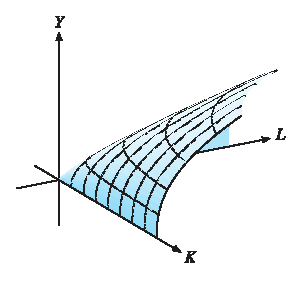
\includegraphics[width=\linewidth]{figure1}\label{fig:1}
			\caption{Gráfica de la función de producción Cobb-Douglas.}
		\end{minipage}
		\hfill
		\begin{minipage}[c]{0.4\linewidth}
			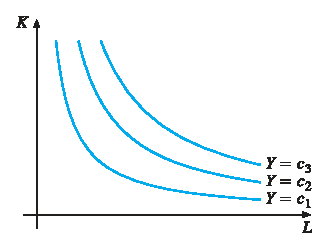
\includegraphics[width=\linewidth]{figure2}\label{fig:2}
			\caption{Isocuantas de la función de producción Cobb-Douglas.}
		\end{minipage}
	\end{figure}
\end{example}
% pag. 428
\begin{example}[Funciones $n$--lineales y $\log$--lineales]
	\leavevmode
	\begin{enumerate}
		\item\label{item:a} La demanda del azúcar en los Estados Unidos durante el período 1929--1936 fue estimado para ser descrito, aproximadamente, por la fórmula \[ x=108.83-6.0294p+0.164w-0.4217t \] donde $x$ es la demanda del azúcar, $p$ es su precio, $w$ es un índice de producción y $t$ es el año (donde $t=0$ corresponde a 1929).
		\item\label{item:b} La siguiente fórmula es una estimación para la demanda de cerveza en el Reino Unido: \[ x=1.058{x}^{0.136}_{1}{x}^{-0.727}_{2}{x}^{0.914}_{3}x^{0.816}_{4}. \]
		Aquí la cantidad demandada, $x$, es una función de cuatro variables: $x_{1}$, el ingreso per cápita, $x_{2}$, el precio de la cerveza, $x_{3}$, índice general de precios de productos básicos y $x_{4}$, la fuerza de la cerveza.
	\end{enumerate}
\end{example}
Las funciones más simples en el ejemplo anterior es la única en la parte~\eqref{item:a}. Las variables $p$, $w$ y $t$ ocurren solo cuando a la primera potencia, y ellas son multiplicadas por constantes, no por cada otra. Tales funciones son llamadas \emph{lineales}. En general
\begin{equation}
f\left(x_{1},x_{2},\ldots,x_{n}\right)=a_{1}x_{1}+a_{2}x_{2}+\cdots+a_{n}x_{n}+b
\end{equation}
donde $a_{1},a_{2},\ldots,a_{n}$ y $b$ son constantes, es una \emph{función lineal} en $n$ variables.

La función en la parte~\eqref{item:b} del ejemplo  es un caso especial de la función general de Cobb-Douglas
\begin{equation}\label{eq:cobbgeneralized}
F\left(x_{1},x_{2},\ldots,x_{3}\right)=A{x}^{a_{1}}_{1}{x}^{a_{2}}_{2}\cdots{x}^{a_{n}}_{n}
\end{equation}
donde $A>0$, $a_{1},\ldots,a_{n}$ son constantes, definidas para $x_{1}>0,x_{2}>0,\ldots x_{n}>0$. Note que al tomar el logaritmo natural a cada lado de~\eqref{eq:cobbgeneralized} resulta
\begin{equation}
\ln F=\ln A+a_{1}\ln x_{1}+a_{2}\ln x_{2}+\cdots+a_{n}\ln x_{n}.
\end{equation}
Esto muestra que la función de Cobb-Douglas es $\log$--lineal, ya que $\ln F$ es una función lineal para $\ln x_{1},\ln x_{2},\ldots,\ln x_{n}$.
% arara: lualatex: { draft: yes }
% arara: lualatex: { draft: yes }
% arara: pythontex
% !arara: biber
% arara: lualatex: { draft: yes }
% arara: lualatex: {
% arara: --> shell: yes,
% arara: --> synctex: yes,
% arara: --> interaction: batchmode
% arara: --> }
% arara: clean: {
% arara: --> extensions:
% arara: --> ['log','aux','out','pytxcode','synctex.gz','toc','bbl','bcf','blg', 'run.xml']
% arara: --> }
\input{cobb-douglas.tex.preamble}
\begin{document}

\maketitle
\include{./contents/spanish/abstract}

\tableofcontents

\include{./contents/spanish/introduction}
\include{./contents/spanish/cobb-douglas}
\include{./contents/spanish/solow}
\include{./contents/spanish/inada}
\include{./contents/spanish/models}
\include{./contents/spanish/deduction}
\include{./contents/spanish/understandingsolow}
\include{./contents/spanish/crecimiento}
%\include{./contents/spanish/codification}
%\include{./contents/spanish/sympying}
%\include{./contents/spanish/references}

\appendix

%\include{./contents/spanish/performance}
%\include{./contents/spanish/linearregression}

\vfill
\begin{flushright}
Facultad de Ciencias, \today.
\end{flushright}

\include{./contents/english/abstract}

\tableofcontents

\vfill
\begin{flushright}
Science department, \today.
\end{flushright}

\end{document}
\section{Introducción}
Cualquier teoría depende de supuestos que no son del todo ciertos. Eso es lo que lo hace teoría. El arte de teorizar con éxito es hacer los supuestos simplificadores inevitables de tal manera que los resultados finales no sean muy sensibles. Una suposición ``crucial'' es una de las cuales las conclusiones dependen sensiblemente, y es importante
que los supuestos cruciales sean razonablemente realistas. Cuando los resultados de una teoría parecen fluir específicamente de una suposición crucial especial, entonces, si la suposición es dudosa, los resultados son sospechosos.

Deseo argumentar que algo así es cierto en el modelo de crecimiento económico Harrod--Domar. La característica y poderosa conclusión de la línea de pensamiento Harrod--Domar es que incluso para el largo plazo, el sistema económico está en el mejor de los casos equilibrado sobre el filo del cuchillo del equilibrio del crecimiento. ¿Eran las magnitudes de los parámetros clave --la relación de ahorro, la relación capital-producto, la tasa de aumento de la mano de obra--si se deslizara un poco desde el punto muerto, la consecuencia sería un desempleo creciente o una inflación prolongada. En términos de Harrod, la cuestión crítica del equilibrio se reduce a una comparación entre la tasa natural de crecimiento que depende, en la ausencia del cambio tecnológico, en el aumento de la fuerza laboral, y la tasa de crecimiento garantizada que depende de los hábitos de ahorro e inversión de los hogares y las empresas.

Pero esta oposición fundamental de tasas garantizadas y naturales al final resulta que parte del supuesto crucial de que la producción tiene lugar en condiciones de \emph{proporciones fijas}. No hay posibilidad de sustituir mano de obra por capital en producción. Si esta suposición se abandona, la noción del filo de cuchillo de equilibrio inestable parece ir con eso. De hecho, no es sorprendente que una rigidez tan grave en una parte del sistema implique falta de flexibilidad en otro.

Una característica notable del modelo Harrod--Domar es que estudia constantemente los problemas a largo plazo con las herramientas de corto plazo habitual. Normalmente se piensa en el largo plazo como el dominio del análisis neoclásico, la tierra del margen. En cambio Harrod y Domar hablan del largo plazo en términos del multiplicador, el acelerador, ``el'' coeficiente de capital. La mayor parte de este documento está dedicado a un modelo de crecimiento a largo plazo que acepta todos los supuestos de Harrod--Domar excepto el de proporciones fijas. En cambio supongo que la única mercancía compuesta es producida por trabajo y capital bajo las condiciones neoclásicas estándar. La adaptación del sistema a una tasa de incremento de la fuerza laboral dada de manera exógena se calcula en algún detalle, para ver si aparece la inestabilidad de Harrod. Las reacciones de interés precio-salario juegan un papel importante en este proceso de ajuste neoclásico, por lo que también se analizan. Luego, algunos de los otros rígidos supuestos se relajan ligeramente para ver qué cambios cualitativos resultan: se permite un cambio tecnológico neutral y un interés elástico horario de ahorro. Finalmente, las consecuencias de ciertas relaciones y rigideces más ``keynesianas'' son brevemente consideran.

\section{Un modelo de crecimiento a largo plazo}
Solo hay una mercancía, la producción como un todo, cuya tasa de producción se designa $Y\left(t\right)$. Así podemos hablar inequívocamente del ingreso real de la comunidad. Parte de cada salida instantánea es consumida y el resto se ahorra e invierte. La fracción de la salida ahorrada es una constante $s$, de modo que la tasa de ahorro es $sY\left(t\right)$. El stock de capital de la comunidad $K\left(t\right)$ toma la forma de una acumulación de la mercancía compuesta. La inversión neta es solo la tasa de
aumento de este capital social $\mathrm{d}K/\mathrm{d}t$ o $\dot{K}$, por lo que tenemos la identidad básica en cada instante de tiempo:
\begin{equation}\label{eq:first}
\dot{K}=sY
\end{equation}
La salida es producida con la ayuda de dos factores de producción, capital y trabajo, cuya tasa de ingreso es $L\left(t\right)$. Las posibilidades tecnológicas son representadas por una función de producción.
\begin{equation}\label{eq:second}
Y=F\left(K,L\right)
\end{equation}
La salida es entendida como la salida neta después de hacer buena la depreciación del capital. Sobre la producción, todo lo que diremos en este momento es que muestra rendimientos constantes a escala. Por lo tanto, la función de producción es homogénea de primer grado. Esto equivale a asumir que no existe un recurso escaso no aumentable como la tierra. Retornos de escala constante parece la suposición natural para hacer en una teoría de crecimiento. El caso de tierras escasas conduciría a rendimientos decrecientes a
escala en capital y trabajo y el modelo se volvería más Ricardiano.

Insertando~\eqref{eq:second} en~\eqref{eq:first} obtenemos
\begin{equation}\label{eq:third}
\dot{K}=sF\left(K,L\right).
\end{equation}
Este es una ecuación con dos incógnitas. Una primera manera de acercarse al sistema sería agregar una ecuación de demanda de trabajo: la productividad física del trabajo marginal es igual a la tasa salarial real; y una ecuación de oferta de trabajo. Este último podría tomar la forma general de hacer trabajo proporcionar una función del salario real, o más clásico de poner el salario real igual a un nivel de subsistencia convencional. En cualquier caso serían tres ecuaciones en las tres incógnitas $K$, $L$, salario real.

En cambio, procedemos más en el espíritu del modelo Harrod. Como un resultado exógeno del crecimiento de la población, la fuerza laboral aumenta a una tasa relativa constante $n$. En ausencia de cambio tecnológico, $n$ es la tasa natural de crecimiento de Harrod. Así:
\begin{equation}\label{eq:fourth}
L\left(t\right)=L_{0}e^{nt}
\end{equation}
En~\eqref{eq:third} $L$ representa el empleo total; en~\eqref{eq:fourth} $L$ representa la oferta de trabajo disponible. Al identificar los dos estamos asumiendo que el empleo se mantiene perpetuamente. Cuando insertamos~\eqref{eq:fourth} en~\eqref{eq:third} obtenemos
\begin{equation}\label{eq:fifth}
\dot{K}=sF\left(K,L_{0}e^{nt}\right)
\end{equation}
tenemos la ecuación básica que determina el camino temporal de la acumulación del capital que debe ser serguida si todas los trabajos disponibles están empleados.

Alternativamente,~\eqref{eq:fourth} puede ser visto como una curva de oferta de mano de obra. Eso dice que la fuerza laboral que crece exponencialmente se ofrece para un empleo completamente inelástico. La curva de oferta de trabajo es una línea vertical que se mueve hacia la derecha en el tiempo a medida que la fuerza laboral crece de acuerdo
para~\eqref{eq:fourth}. Luego, la tasa salarial real se ajusta para que toda la mano de obra disponible sea empleado, y la ecuación de productividad marginal determine la tasa salarial que realmente gobernará.

En resumen,~\eqref{eq:fifth} es una ecuación diferencial con la única variable $K\left(t\right)$. Su solución da el único perfil de tiempo del capital social de la comunidad que empleará plenamente la mano de obra disponible. Una vez que nosotros conozca el camino temporal del stock de capital y el de la fuerza laboral, podemos calcular desde la función de producción la ruta de tiempo correspondiente de salida real. La ecuación de productividad marginal determina la trayectoria temporal del salario real. También hay una suposición involucrada de pleno empleo del stock de capital disponible. En cualquier punto de tiempo en que el stock de capital preexistente (el resultado de una acumulación previa) se suministra de manera inelástica. Por lo tanto, existe una ecuación de productividad marginal similar para el capital que determina el alquiler real por unidad de tiempo para los servicios de capital social. El proceso puede ser visto de esta manera: en cualquier momento la oferta laboral disponible está dado por~\eqref{eq:fourth} y el stock de capital disponible también es un dato. Ya que el rendimiento real de los factores se ajustará para lograr el pleno empleo de trabajo y capital podemos usar la función de producción~\eqref{eq:second} para encontrar la tasa actual de salida. Entonces la propensión a ahorrar nos dice cuánto de la producción neta se ahorrará e invertirá. Por eso conocemos la acumulación del capital neta durante el período actual. Agregado al stock ya acumulado, esto da el capital disponible para el próximo período, y todo el proceso puede repetirse.
\section{Posibles patrones de crecimiento}
Para ver si siempre existe una ruta de acumulación de capital consistente con cualquier tasa de crecimiento de la fuerza laboral, debemos estudiar la ecuación diferencial~\eqref{eq:fifth} por la naturaleza cualitativa de sus soluciones. Naturalmente sin especificar la forma exacta de la función de producción no podemos esperar encontrar la solución exacta. Pero ciertas propiedades amplias son sorprendentemente fáciles de aislar, incluso gráficamente.

Para ello, introducimos una nueva variable $r=\frac{K}{L}$, la relación de capital al trabajo Por lo tanto, tenemos $K=rL=rL_{0}e^{nt}$. Diferenciando con respecto al tiempo que tenemos
\begin{equation}
\dot{K}=L_{0}e^{nt}r^{\prime}+nrL_{0}e^{nt}.
\end{equation}
Reemplazando esto en~\eqref{eq:fifth}: \[ \left(\dot{r}+nr\right)L_{0}e^{nt}=sF\left(K,L_{0}e^{nt}\right). \] Pero debido al retorno de escala constante podemos dividir ambas variales en $F$ por $L=L_{0}e^{nt}$, no obstante, multiplicamos $F$ por el mismo factor. Así \[ \left(\dot{r}+nr\right)L_{0}e^{nt}=sLe^{nt}F\left(\frac{K}{L_{0}e^{nt}},1\right) \] y dividiendo el factor común llegamos finalmente a
\begin{equation}\label{eq:sixth}
\dot{r}=sF\left(r,1\right)-nr.
\end{equation}
Aquí tenemos una ecuación diferencial que involucra solamente la relación capital-trabajo.

Esta ecuación fundamental se puede alcanzar menos formalmente. Como $r=\frac{K}{L}$, la tasa de cambio relativa de $r$ es la diferencia entre las tasas relativas de cambio de $K$ y $L$. Eso es: \[ \frac{\dot{r}}{r}=\frac{\dot{K}}{K}-\frac{\dot{L}}{L}. \] Ahora primero que nada $\frac{\dot{L}}{L}=n$. En segundo lugar, $\dot{K}=sF\left(K,L\right)$. Haciendo estas substituciones: \[ \dot{r}=r\frac{sF\left(K,L\right)}{K}-nr. \] Ahora divida $L$ de $F$ como antes, note que que $\frac{L}{K}=\frac{1}{r}$ y obtenemos~\eqref{eq:sixth} nuevamente.

La función $F\left(r,1\right)$ que aparece en~\eqref{eq:sixth} es fácil de interpretar. Esta es la curva del producto total cuando varían las cantidades $r$ de capital con una unidad de trabajo. Alternativamente, da salida por trabajador como una función de capital por trabajador. Así~\eqref{eq:sixth} establece que la tasa del cambio de la relación capital-trabajo es la diferencia de dos términos, uno representando el incremento de capital y uno el incremento de trabajo.

Cuando $\dot{r}=0$, la relación capital-trabajo es una constante, y el capital existente debe expandirse al mismo ritmo que la fuerza laboral, es decir, $n$.

(La tasa de crecimiento garantizada, garantizada por la tasa real apropiada de retorno al capital, es igual a la tasa natural.) En la Figura I, el rayo que pasa por el origen con pendiente $n$ representa la función $nr$. La otra curva es la función $sF\left(r,1\right)$. Aquí se dibuja para pasar por el origen y convexo hacia arriba: sin salida a menos que ambas entradas sean positivas, y la disminución de la productividad marginal del capital, como sería el caso, por ejemplo, con la función Cobb-Douglas. En el punto de intersección $nr=sF\left(r,1\right)$ y $\dot{r}=0$. Si la relación capital-trabajo $r^{\ast}$ debe establecerse, se mantendrá, y el capital y
el trabajo crecerá de allí en adelante en proporción. Por la constante retornos a escala

\newpage
Formalmente, una función de producción se define para tener:
\begin{itemize}
	\item Constante retorno a escala si (para cualquier constante $a$ es mayor que $0$) $F\left(aK,aL\right)=aF\left(K,L\right)$ (Función $F$ es homogénea de grado $1$).
	\item Retornos a escala crecientes si (para cualquier constante mayor que $1$) $F\left(aK,aL\right)>aF\left(K,L\right)$.
	\item Retornos a escala decrecientes si (para cualquier constante $a$ mayor que $1$) $F\left(aK,aL\right)<aF\left(K,L\right)$.
\end{itemize}
donde $K$ y $L$ son factores de producción--capital y trabajo, respectivamente.

En una configuración más general, para procesos de producción de múltiples entradas y múltiples salidas, se puede suponer que la tecnología se puede representar a través de algún conjunto de tecnología, llámelo $T$ que debe satisfacer algunas condiciones de regularidad de la teoría de la producción. En este caso, la propiedad de retorno de escala constante es equivalente a decir que el conjunto tecnológico es un cono, es decir, satisface la propiedad $aT=T$, $\forall a>0$. A su vez, si hay una función de producción que describirá el conjunto de tecnología $T$, deberá ser homogéneo de grado $1$.


\begin{definition}[Rendimiento de escala]
	La forma funcional de Cobb-Douglas tiene una constante retorno de escala cuando la suma de sus exponentes es $1$. En este caso, la función es
	\begin{equation}
	F\left(K,L\right)=AK^{b}L^{1-b}
	\end{equation}
	donde $A>0$ y $0<b<1$. Así \[ F\left(aK,aL\right)=A{\left(ak\right)}^{b}{\left(aL\right)}^{1-b}=Aa^{b}a^{1-b}K^{b}L^{1-b}=aAK^{b}L^{1-b}=aF\left(K,L\right). \] Aquí como entrada usamos todas las escalas por un factor multiplicador $a$, la salida también escala por $a$ y así existen constantes de retorno de escala.
	
	Pero, si la función de producción de Cobb-Douglas tiene su forma general
	\begin{equation}
	F\left(K,L\right)=AK^{b}L^{c}
	\end{equation}
	donde $0<b<1$ y $0<c<1$, entonces existen retornos crecientes si $b+c>1$, pero retornos decrecientes si $b+c<1$, dado que \[ F\left(aK,aL\right)=A{\left(aK\right)}^{b}{\left(aL\right)}^{c}=Aa^{b}a^{c}K^{b}L^{c}=a^{b+c}AK^{b}L^{c}=a^{b+c}F\left(K,L\right), \] que para $a>1$ es mayor que o menor que $aF\left(K,L\right)$ cuando $b+c$ es mayor o menor que uno.
\end{definition}

Hay dos clases especiales de funciones de producción que a menudo se analizan. La función de producción $Q=f\left(X_{1},X_{2},\ldots,X_{n}\right)$ se dice que es homogéneo de grado $m$, si se le da alguna constante positiva $k$, $f\left(kX_{1},kX_{2},\ldots,kX_{n}\right)=k^{m}f\left(X_{1},X_{2},\ldots, X_{n}\right)$. Si $m>1$, la función exhibe rendimientos crecientes a escala, y exhibe rendimientos decrecientes a escala si $m<1$. Si es homogéneo de grado $1$, exhibe rendimientos constantes a escala. La presencia de rendimientos crecientes significa que un aumento del uno por ciento en los niveles de uso de todas las entradas daría como resultado un aumento de más del uno por ciento en la producción; la presencia de rendimientos decrecientes significa que daría como resultado un aumento de producción de menos del uno por ciento. Los retornos constantes a escala son el caso intermedio. En la función de producción Cobb–Douglas mencionada anteriormente, los rendimientos a escala aumentan si $a_{1}+a_{2}+\cdots+a_{n}> 1$, disminuyendo si $a_{1}+a_{2}+\cdots+a_{n}<1$, y constante si $a_{1}+a_{2}+\cdots+a_{n}=1$.

Si una función de producción es homogénea y de grado uno, este a veces llamada ``linealmente homogénea''. Una función de producción linealmente homogénea con entradas capital y labor tienen las propiedades de que los productos físicos marginales y promedio tanto del capital como del trabajo pueden expresarse solamente como funciones de la relación capital-trabajo. Además, en este caso, si cada entrada se paga a una tasa igual a su producto marginal, los ingresos de la empresa se agotarán exactamente y no habrá ganancias económicas excesivas.

Las funciones homotéticas son funciones cuya tasa de sustitución técnica marginal (la pendiente de la isocuanta, una curva dibujada a través del conjunto de puntos en dicho espacio de trabajo-capital en el que se produce la misma cantidad de producción para combinaciones variables de las entradas) es homogénea de grado cero Debido a esto, a lo largo de los rayos que provienen del origen, las pendientes de las isocuantas serán las mismas. Las funciones homotéticas tienen la forma $F\left(h\left(X_{1},X_{2}\right)\right)$ donde $F(y)$ es una función monótona creciente (la derivada de $F\left(y\right)$ es positiva $\mathrm{d}F/\mathrm{d}y>0$, y la función $h\left(X_{1},X_{2}\right)$ es una función homogénea de cualquier grado.

La elasticidad de sustitución constante (CES), en economía, es una propiedad de algunas funciones de producción y funciones de utilidad.

Específicamente, este en un tipo particular de función agregado que combina dos o más tipos de productos de consumos, o dos o más tipos de entradas de producción dentro de un cantidad agregado. Esta función de agregación exhibe una elasticidad de sustitución constante.
\begin{definition}[Elasticidad de sustitución constante]
La función de producción CES es una función de producción neoclásica que muestra una elasticidad de sustitución constante. En otras palabras, la producción tecnológica tiene un porcentaje de cambio constante en factores (por ejemplo, trabajo y capital) proporcional debido al cambio porcentual en la tasa marginal de la sustitución técnica. Los dos factores (capital y trabajo) de la función de producción fue introducido por Solow y más tarde popularizado por Arrow, Chenery, Minhas y Solow es
\begin{equation}
Q=F\cdot{\left(a\cdot K^{\rho}+\left(1-a\right)\cdot L^{\rho}\right)}^{\frac{v}{\rho}}
\end{equation}
donde
\begin{itemize}
	\item $Q$ es la cantidad de salida,
	\item $F$ es el factor de productividad,
	\item $a$ es el parámetro forma,
	\item $K,L$ son las cantidades de los factores de producción primario (capital y trabajo)
	\item $\rho=\frac{\sigma-1}{\sigma}$ es el parámetro de sustitución,
	\item $\sigma=\frac{1}{1-\rho}$ es elasticidad de sustituación,
	\item $v$ es el grado de homogeneidad de la función de producción. Donde $v=1$ es el retorno de escala constante, $v<1$ es el retorno de escala decreciente y $v>1$ es el retorno de escala creciente.
\end{itemize}
Como su nombre lo sugiere, la función de producción CES exhibe una elasticidad de sustitución constante entre el capital y el trabajo. Leontief, linear y las funciones de Cobb-Douglas son casos especiales de la función de producción CES. Esto es,
\begin{itemize}
	\item Si $\rho$ se aproxima a $1$, tenemos una lineal o función de sustituto perfecto.
	\item Si $\rho$ se aproxima a cero en el límite, obtenemos la función de producción de Cobb-Douglas.
	\item Si $\rho$ se aproxima al menos infinito, obtenemos la Leontief o función de producción perfecta complementaria.
\end{itemize}
La forma general de la función de producción CES, con $n$ entradas, es
\begin{equation}
Q=F\cdot{\left[\sum_{i=1}^{n}a_{i}X^{r}_{i}\right]}^{\frac{1}{r}}
\end{equation}
donde
\begin{itemize}
	\item $Q$ es cantidad de salida
	\item $F$ es el factor de productividad
	\item $a_{i}$ es el parámetro forma de la entrada $i$, $\sum_{i=1}^{n}a_{i}=1$
	\item $X_{i}$ son las cantidades de los factores de producción, $i=1,2,\ldots,n$.
	\item $s=\frac{1}{1-r}$ es la elasticidad de sustitución.
\end{itemize}
\end{definition}
Extendiendo la forma función CES (Solow) para acomodar los múltiples factores de producción crea algunos problemas. Sin embargo, no existe una forma completamente general para hacer esto. Uzawa mostró que solo $n$ factores posibles de la función de producción $n>2$ con elasticidades de sustitución parciales constantes requiere o todas las elasticidades entre pares de factores son idénticas, o si alguna difiere, todo ellos deben ser igual a cada otra y todas las elasticidades restantes deben ser unitarias. Esto es verdad para cualquier función de producción. Esto significa el uso de la forma funcional CES para más dos factores significará general que no existe una elasticidad de sustitución entre todos los factores.

Las funciones CES anidades son comúnmente encontradas en los modelos de equilibrio parcial y equilibrio general. Diferentes anidamientos (niveles) permiten la introducción de las elasticidades de sustitución apropiadas.

\begin{definition}[Función de utilidad CES]
La misma forma funcional CES alcanza como una función de utilidad en la teoría del consumidor. Por ejemplo, si existen $n$ tipos de productos de consumos $x_{i}$, entonces el consumo agregado $X$ podría definirse usando el agregado CES:
\begin{equation}
X={\left[\sum_{i=1}^{n}a^{\frac{1}{s}}_{i}x^{\frac{s}{s-1}}_{i}\right]}^{\frac{s}{s-1}}
\end{equation}
Aquí nuevamente, los coeficientes $a_{i}$ son los parámetros forma y $s$ es la elasticidad de sustitución. Por lo tanto, los productos de consumo $x_{i}$ son perfectos sustitutos cuando $s$ se aproxima al infinito y complemento perfecto cuando $s$ se aproxima a cero. El agregado CES es también algunas veces llamado el \emph{agregador Armington}, el cual fue discutido por Armington (1969).

Las funciones de utilidad CES son un caso especial de las preferencias homotéticas.

El siguiente es un ejemplo de la función de utilidad CES para dos productos, $x$ e $y$ con igualdad compartidad:
\begin{equation}
u\left(x,y\right)={\left(x^{r}+y^{r}\right)}^{1/r}.
\end{equation}
La función expendidora en el caso es:
\begin{equation}
e\left(p_{x},p_{y},u\right)={\left(p^{r/\left(r-1\right)}_{x}+p^{r/\left(r-1\right)}_{y}\right)}^{\left(r-1\right)/r}\cdot u.
\end{equation}
La función de utilidad indirecta tiene su inversa:
\begin{equation}
v\left(p_{x},p_{y},I\right)={\left(p^{r/\left(r-1\right)}_{x}+p^{r/\left(r-1\right)}_{y}\right)}^{\left(1-r\right)/r}\cdot I.
\end{equation}
La funciones de demanda son:
\begin{align*}
x\left(p_{x},p_{y},I\right)
&=\frac{p^{1/\left(r-1\right)}_{x}}{p^{r/\left(r-1\right)}_{x}+p^{r/\left(r-1\right)}_{y}}\cdot I\\
y\left(p_{x},p_{y},I\right)
&=\frac{p^{1/\left(r-1\right)}_{y}}{p^{r/\left(r-1\right)}_{x}+p^{r/\left(r-1\right)}_{y}}\cdot I\\
\end{align*}
La función de utilidad CES es uno de los casos considerados por Dixit y Stiglitz (1977) en su estudio de la diversidad del producto optimal en el contexto de la competición monopolística.

Note que la diferencial entre la utilidad CES y la utilidad isoelástica: La función de utilidad CES es una función de utilidad ordinal que representa las preferencias sobre consumo seguro %TODO: Wikipedia https://en.wikipedia.org/wiki/Constant_elasticity_of_substitution
mientras que la función de utilidad isoelástica es una función de utilidad cardinal que representa en loterías. Una función de utilidad CES indirecta (dual) ha sido usado para derivar la marca de consistencia-utildidad de sistemas donde la demanda categórica son determinadas endógenamente por un multicategorizador, la función de utilidad CES indirecto. Esto también se ha muestro que las preferencias son autoduales y ambos son primales y duales % TODO:
podrían exhibir cualquier grado de convexidad.
\end{definition}
La existencia y la estabilidad relativa de un único crecimiento balanceado para modelos multisectoriales fueron establecidos por Solow y Samuelson bajo el supuesto de \emph{retorno de escala constante}. Ellos estudiaron dos tipos de sistemas de ecuaciones: el sistema de ecuación en \emph{diferencias} y el sistema de ecuación diferencial. Later Muth y Suit estudiaron el sistema formado bajo el supuesto de retorno de escala decreciente. El primer objetivo de este artículo es estudiar algún sistema de ecuación diferencial bajo los supuestos más débiles que los impuestos por Solow y Samuelson, pero que retenga el supuesto de \emph{retorno constante} de escala. El segundo objetivo es investigar cierto sistema de ecuación diferencial bajo el supuesto de \emph{retorno de escala decreciente}.

\subsection{Retorno de escala constante -- Caso general}
Nuestro sistema es expresado por las siguientes ecuaciones:
\begin{equation}
\dot{X}_{i}=H^{i}\left(X_{1},\ldots,X_{n}\right),\quad\left(i=1,\ldots,n\right).
\end{equation}
El sistema de arriba es modelo de crecimiento balanceado de Solow--Samuelson. Los $H^i$'s son definidos para cualquier $\left(X_{1},\ldots,X_{n}\right)\geq0$ y son asumidos que son continuas con respecto a cualquier variable y positivamente homogénea de grado uno. A lo largo del artículo, los $X_{i}$'s son restringidos a valores no negativos. Además, las funciones son solo definidas para valores no negativos. Esto es asumido que
\begin{equation}
H^{i}\text{ es no decreciente en todas las variables, excepto en }X^{i},
\end{equation}
y que
\begin{equation}
\left\{H^{1},\ldots,H^{n}\right\}\text{ es indescomponible}.
\end{equation}
Aquí la indescomposibilidad es definido como en Morishima. Esto es, para cualquier conjunto de índices $R=\left\{i_{i},\ldots,i_{r}\right\}$, las relaciones $X_{i}=X^{\prime}_{i}$ para $i\in R$ y $X_{l}<X^{\prime}_{l}$ para $l\notin R$ implica que existe por lo menos un $i\in R$ tal que $H^{i}\left(X_{1},\ldots,X_{n}\right)<H^{i}\left(X^{\prime}_{i},\ldots,X^{\prime}_{n}\right)$. Requerimos que $H^{i}$ sea no decreciente en $X_{j}$, para $j\neq i$, sin la restricción sobre la dependencia de $H^{i}$ sobre $X_{i}$. En contraste del supuesto de Solow y Samuelson que $H^{i}$ es creciente en todos los $X_{j}$.

Ddas sus supuestos y la homogeneidad de $H^{i}$ $\left(i=1,\ldots,n\right)$, este sigue que $H^{i}\geq0$ $(i=1,\ldots,n)$ para $X_{j}\geq0$ $(j=1,\ldots,n)$, y que, $H^{i}=0$  para todo $i$, si y solo si $X_{j}=0$ para todo $j$. En nuestro caso, sin embargo, $H^{i}$ no es necesariamente creciente en $X$. Por ello, no podemos obtener las propiedades mencionadas arriba. Así, asumimos ellos. Esto es, podemos asumir que
\begin{equation}
H^{i}\geq0\quad(i=1,\ldots,n)\text{ para }X_{j}\geq0\quad\left(j=1,\ldots,n\right).
\end{equation}
Entonces, de la indescomposabilidad y la homogeneidad de $H^{i}$, $H^{i}=0$ para todo $i$, si y solo si $X_{j}=0$ para todo $j$. Nuestro ánimo es probar el siguiente teorema.

\begin{theorem}
	Para el sistema de ecuaciones diferenciales, %TODO
	existe un único determinado positivo autovalor, estrictamente un único positivo autovector normalizado y así un único camino de crecimiento balanceado. Más aún, cualquier solución del camino del sistema relativamente se aproxima al camino de crecimiento balanceado.
\end{theorem}
\begin{proof}
Podemos mostrar por un procedimiento similar al de Solow y Samuelson sobre la existencia de un autovalor positivo $\lambda$ y un autovector no negativo, no nulo $V=\left(V_{1},V_{2},\ldots,V_{n}\right)$ tal que
\begin{align*}
\lambda V_{1}&=H^{1}\left(V_{1},\ldots,V_{n}\right),\\
&=\vdots\\
\lambda V_{n}&=H^{n}\left(V_{1},\ldots,V_{n}\right).
\end{align*}
Mostraremos que \emph{todas las componentes del autovector} $V$ \emph{son positivas}. Suponga que algunas componentes de $V$ son ceros. Sin pérdida de generalidad, podríamos suponer que \[ V_{i}=0\quad\text{para }i\leq r(<n), \] y \[ V_{i}>0\quad\text{ para }n\geq i>r. \] Entonces,
\begin{align*}
0&=H^{1}\left(0,\ldots0,V_{r+1},\ldots,V_{n}\right),\\
&=\vdots
0&=H^{r}\left(0,\ldots0,V_{r+1},\ldots,V_{n}\right),\\
0<\lambda V_{r+1}&=H^{r+1}\left(0,\ldots0,V_{r+1},\ldots,V_{n}\right),\\
&=\vdots
0<\lambda V_{n}&=H^{n}\left(0,\ldots0,V_{r+1},\ldots,V_{n}\right).
\end{align*}
Pero esto contradice la suposición de indescomposabilidad, así es fácilmente visto haciendo
\begin{align*}
R\equiv\left\{1,\ldots,r\right\},\\
\left(X_{1},\ldots,X_{r},X_{r+1},\ldots,X_{n}\right)
&\equiv\left(0,\ldots0,V_{r+1},\ldots,V_{n}\right),\\
\left(X^{\prime}_{1},\ldots,X^{\prime}_{r},X^{\prime}_{r+1},\ldots,X^{\prime}_{n}\right)
&=\equiv\left(0,\ldots0,2V_{r+1},\ldots,2V_{n}\right).
\end{align*}
Ahora, mostraremos la unicidad del autovalor. Suponga que existe otra \emph{tupla}de un autor valor positivo y un autovector $\left(\mu, U\right)$. Entonces obtenemos los siguientes conjuntos de relaciones
\begin{align}
\lambda&=H^{1}\left(1,\frac{V_{2}}{V_{1}},\ldots,\frac{V_{n}}{V_{1}}\right),\\
\lambda&=H^{2}\left(\frac{V_{1}}{V_{2}},1,\ldots,\frac{V_{n}}{V_{2}}\right),\\
&=\vdots\\
\lambda&=H^{n}\left(\frac{V_{1}}{V_{n}},\frac{V_{2}}{V_{n}},\ldots,1\right),\\
\mu&=H^{1}\left(1,\frac{U_{1}}{U_{2}},\ldots,\frac{U_{n}}{U_{1}}\right),\\
\mu&=H^{2}\left(\frac{U_{1}}{U_{n}},\frac{U_{2}}{U_{n}}\ldots,1\right).
\end{align}
Asuma que $\lambda>\mu$. Compare %TODO:.
Entonces, \[ H^{1}\left(1,\frac{V_{2}}{V_{1}},\ldots,\frac{V_{n}}{V_{1}}\right)>H^{1}\left(1,\frac{U_{2}}{U_{1}},\ldots,\frac{U_{n}}{U_{1}}\right). \] Dado que $H^{1}$ es no decreciente en todos los argumentos, excepto en el primero, podemos reemplazar $i=2$. Esto es,
\begin{equation}
\frac{V_{2}}{V_{1}}>\frac{U_{2}}{U_{1}}.
\end{equation}
Compare %TODO:
Entonces, \[ H^{2}\left(\frac{V_{1}}{V_{2}},1,\ldots,\frac{V_{n}}{V_{2}}\right)>H^{2}\left(\frac{U_{1}}{U_{2}},1,\ldots\frac{U_{n}}{U_{2}}\right). \] Dado que $V_{1}/V_{2}<U_{1}/U_{2}$, y $H^{2}$ es no decreciente en todos los argumentos, excepto en el segundo, debemos tener, digamos,
\begin{equation}
\frac{V_{3}}{V_{2}}>\frac{U_{3}}{U_{2}}.
\end{equation}
De %TODO:
obtenemos $V_{1}/V_{3}<U_{1}/U_{3}$ y $V_{2}/V_{3}<U_{2}/U_{3}$. Continuando con este razonamiento, alcanzamos una contradicción para las últimas relaciones %TODO:

Dado que los argumentos diagonales en el lado de derecho de ambos grupos de relaciones son todos uno, no necesitamos asumir que $H^{i}$ es creciente en $X^{i}$. El razonamiento de arriba ha sido alcanzado usado por Solow y Samuelson para mostrar la unicidad de los autovalores para el caso $n=2$. Pero ellos usan diferentes razonamientos para el caso general. En este razonamiento, ellos usan la propiedad que $H^{i}$ es creciente en $X_{j}$.

Notamos también que el razonamiento de arriba es usado por Solow y Samuelson para mostrar la unicidad del vector normalizado y que el \emph{procedimiento es aplicable con un ligera modificación en nuestro caso también}. Así, podemos omitir la prueba de $V=\alpha U$. Aquí, $\alpha$ es una constante de proporcionalidad.

Nuestro siguiente objetivo es \emph{mostrar que la estabilidad relativa del camino dinámico}.

Definimos nuevas variables,
\begin{equation}
y_{i}=\frac{X_{i}}{V_{i}e^{\lambda t}},\quad\left(i=1,\ldots,n\right).
\end{equation}
Entonces, \[ y_{i}V_{i}e^{\lambda t}=X_{i}. \] Diferenciando ambos lados de esta relación, obtenemos
\begin{equation}
\dot{y}V_{i}e^{\lambda t}+\lambda y_{i}V_{i}e^{\lambda t}=\dot{X}_{i}\quad\left(i=1,\ldots,n\right).
\end{equation}
Sustituyendo las relaciones %TODO:
dentro del sistema original, obtenemos
\begin{equation}
\dot{y}_{i}=H^{i}\left(\frac{V_{1}}{V_{i}}y_{1},\ldots,\frac{V_{n}}{V_{i}}y_{n}\right)-\lambda y_{i},\quad\left(i=1,\ldots,n\right).
\end{equation}
Ponga \[ \min\left\{y_{i}\left(t\right)\right\}=m\left(t\right)=y_{k_{1}}\left(t\right)=\cdots=y_{k_{r}}\left(t\right), \] y suponga que \[ y_{\ell}\left(t\right)>m\left(t\right)\quad\text{para }\ell\neq k_{j}. \] Entonces, \[ \dot{y}_{k_{j}}\left(t\right)\geq0\quad\text{ para todo }j\leq r \] y \[ \dot{y}_{k_{j}}\left(t\right)>0\quad\text{ para al menos un }j\leq r. \] Esto es mostrado como sigue.
\begin{align*}
\dot{y}_{k_{j}}
&=H^{k_{j}}\left(\frac{V_{1}}{V_{k_{j}}}y_{1},\ldots,\frac{V_{n}}{V_{k_{j}}}y_{n}\right)-\lambda y_{k_{j}}\\
&\geq H^{k_{j}}\left(\frac{V_{1}}{V_{k_{j}}}m\left(t\right),\ldots,\frac{V_{n}}{V_{k_{j}}}m\left(t\right)\right)-\lambda m\left(t\right)\\
&=m\left(t\right) H^{k_{j}}\left(\frac{V_{1}}{V_{k_{j}}},\ldots,\frac{V_{n}}{V_{k_{j}}}\right)-\lambda m\left(t\right)=0,\quad\text{ para }j=1,\ldots,r.
\end{align*}
Pero la desigualdad se mantiene para al menos un $k_{j}$. Esto sigue de la suposición de indescomposibilidad si ponemos
\begin{align*}
R&\equiv\left\{k_{1},\ldots,k_{r}\right\}\\
\left(X_{1},\ldots X_{n}\right)
&=\left(V_{1}m\left(t\right),\ldots,V_{n}m\left(t\right)\right)
\shortintertext{y}
\left(X^{\prime}_{1},\ldots,X^{\prime}_{n}\right)
&=\left(V_{1}y_{1},\ldots,V_{n}y_{n}\right).
\end{align*}
Con esta propiedad, inferimos que el mínimo valor de $y_{i}\left(t\right)$ no puede mantenerse constante por siempre. Para, cada momento de tiempo, el número de mínimos $y_{k}\left(t\right)$0s es decreciente. Eventualmente, existe solo un mínimo $y_{k}\left(t\right)$. %TODO: Henceforth
Por ello, el mismo mínimo debe incrementar. Dado que el lapso de tiempo continuamente en nuestro caso, $m\left(t\right)$ siempre incrementa sobre el tiempo, provisto que $y_{\ell}\left(t\right)>m\left(t\right)$ para al menos un $\ell$. Esto es posible que \[ \frac{dm\left(t\right)}{dt}=0, \] en un cierto punto. Pero $m\left(t\right)$ se mantiene constante solo por un corto periodo infinitesimal. Eso no hace el residuo estacionario para un periodo finito. La figura 1 muestra la situación. Ponga \[ \max_{i}\left\{y_{i}\left(t\right)\right\}=M\left(t\right). \] Entonces, podemos mostrar que $M\left(t\right)$ decrece, provisto por $Y_{\ell}\left(t\right)<M\left(t\right)$ para al menos un $\ell$.

Así, $m\left(t\right)$ incrementa y converge a un cierto valor positivo $m^{\ast}$ y $M\left(t\right)$ decrece y converge a cierto valor positivo $M^{\ast}$. Esto es,
\begin{align*}
\lim_{t\to\infty}m\left(t\right)
&=m^{\ast}.\\
\lim_{t\to\infty}M\left(t\right)
&=M^{\ast}.
\end{align*}
Entonces,
\[ m^{\ast}\leq M^{\ast}. \] Tenemos que probar que \[ m^{\ast}=M^{\ast}. \] Suponga que $m^{\ast}<M^{\ast}$. Considere un conjunto de vectores en el espacio $n$--dimensional que \[ S\equiv\left\{y\equiv\left(y_{1},\ldots,y_{n}\right)\right\}:\min_{i}y_{i}=m^{\ast}\text{ y }\max_{i}y_{i}=M^{\ast}. \] Este es un conjunto compacto. Considere un camino dinámico que empieza de un punto en este conjunto. Entonces, por el mismo razonamiento de arriba, el mínimo valor de los $y_{i}$'s incrementa y el máximo valor de los $y_{i}$'s decrece. Para hacer explícito esa dependencia en el valor inicial de $y$ en $S$, escribimos, respectivamente, \[ m^{\ast}\left(t;y\right)\text{ y }M^{\ast}\left(t,y\right). \] Luego, \[ m^{\ast}\left(\tau,y\right)>m^{\ast}\left(0,y\right)=m^{\ast}\text{ y }M^{\ast}\left(\tau, y\right)<M^{\ast}\left(0,y\right)=M^{\ast}. \] Aquí, $\tau$ es un valor positivo arbitrariamente escogido. Pero,
\begin{align*}
\inf_{y\in S}\left\{m^{\ast}\left(\tau,y\right)-m^{\ast}\left(0,y\right)\right\}
&=\varepsilon
\shortintertext{y}
\inf_{y\in S}\left\{M^{\ast}\left(0,y\right)-M^{\ast}\left(\tau,y\right)\right\}
&=\delta.
\end{align*}
Dado que $S$ es compacto, tanto $\varepsilon$ como $\delta$ son positivos.

Ahora, volvamos al camino dinámico original. Como se muestra arriba, el $\min_{i} y_{i}\left(t\right)=m\left(t\right)$ y el $\max_{i}y_{i}\left(t\right)=M\left(t\right)$, respectivamente, son suficientemente cercanas a $m^{\ast}$ y $M^{\ast}$ para cualquier $t\geq T$, provisto $T$ es tomado suficientemente grande. Entonces, cualquier punto en el camino dinámico es suficientemente cercano al punto en $S$. De la continuidad de los $H^{i}$'s.
\begin{align*}
m\left(t+\tau\right)-m\left(t\right)>\frac{\varepsilon}{2}
&>0
\shortintertext{y}
M\left(t\right)-M\left(t+\tau\right)>\frac{\delta}{2}
&>0
\end{align*}
para $t\geq T$, provisto $T$ es suficientemente grande. Pero esto contradice \[ \lim_{t\to\infty}m\left(t\right)=m^{\ast}\quad\text{y}\quad\lim_{t\to\infty}M\left(t\right)=M^{\ast}. \] Por lo tanto, \[ m^{\ast}=M^{\ast}. \] Este es el resultado deseado. Esto es notado aquí que todos los componentes del punto inicial $X\left(0\right)$ son no negativos y por lo menos uno de ellos es positivo, entonces esta propiedad se mantiene para cualquier punto $X\left(t\right)$ para todo $t\geq0$.

También es notado aquí que el razonamiento desarrollado arriba no es válido para el sistema de ecuaciones en diferencias \[ X_{i}\left(t+1\right)=H^{i}\left(X_{1}\left(t\right),\ldots,X_{n}\left(t\right)\right),\quad\left(i=1,\ldots,n\right). \] Esto es, si $H^{i}$ es creciente en $X_{i}$, podemos construir un ejemplo en el cual el sistema de ecuación en diferencia es inestable. Morishima tiene mostrado la estabilidad relativa del sistema de ecuación en diferencia bajo el supuesto que $H^{i}$'s son no decrecientes en todos los $X_{j}$'s y $\left(H^{1},\ldots,H^{n}\right)$ es indescomponible y primitivo, es decir, el supuesto de decrecentabilidad del $H^{i}$ en $X^{i}$ y la primitivdad son adcionalmente requeridas.

La estabilidad es mostrada como nuestro incluso sin la suposición de la primitividad. La indescomposibilidad es suficiente. Pero, aquí nuevamente la estabilidad no es obtenida para el sistema de ecuación en diferencia sin el supuesto de primitiidad, esto es, podemos contruir un ejemplo en el cual la inestabilidad es mostrada con la indescomposibilidad pero sin la primitividad. Resumiendo los resultados, la estabilidad es mostrada para el sistema de ecuación diferencial sin los supuestos de no decresabilidad del $H^{i}$ en $X^{i}$ y la primitivdad.

La razón por qué podemos relajar estos supuestos para el sistema de ecuación diferencial, pero no para el sistema de ecuación en diferencias será explicado en la siguiente sección.
\end{proof}

\section{Retorno de escala constante -- Caso matricial}

Nuestro sistema en el caso es
\begin{equation}
\dot{X}=AX.
\end{equation}
Aquí, $X$ es un vector cuyas componentes son los $X_{i}$'s. $A$ es una matriz indescomponible del cual los elementos de su diagonal son asumidos todos no negativos. Esto es, $A$ es una matriz Metzler %TODO: Buscar qué significa eso.
El siguiente teorma es provisto en esta sección.

\begin{theorem}
Para el sistema de ecuación diferencial%TODO: 
bajo la suposición que todos los elementos de su diagonal de $A$ son no negativos, y $A$ es indescomponible, existe un único camino del crecimiento balanceado o decaimiento, y cualquier camino solución se aproxima relativamente a este.

Note que el tasa de ``crecimiento'' puede ser negativo.

\begin{proof}
	Sea $\alpha$ un número positivo que es mayor que el valor absoluto de cualquier elemento de la diagonal de la matriz $A$. Ponga \[ B\equiv A+\alpha I. \] Aquí, $I$ es la matriz identidad. Entonces, todos los elementos de $B$ son negativos y $B$ es indescomponible. Entonces, $B$ tiene un único autovalor positivo $\mu_{1}$ y un único autovector positivo $\overline{X}^{(1)}$ associado con este tal que $\mu_{1}$ no es mayor que los valores absolutos de otros autovalores $\mu_{i}$'s $(i=2,\ldots,n)$ de la matriz $B$. Ahora, es fácilmente ver que el $\mu_{i}-\alpha(\equiv\lambda_{i})$ son autovalores de $A$. Para
	\begin{align*}
	\mu_{i}{\overline{X}}^{(i)}&=B{\overline{X}}^{(i)}=\left(A+\alpha I\right){\overline{X}}^{(i)},
	\shortintertext{y además}
	\lambda_{i}{\overline{X}}^{(i)}&=\left(\mu_{i}-\alpha\right){\overline{X}}^{(i)}=A{\overline{X}}^{(i)}.
	\end{align*}
	Aquí, $\overline{X}^{(i)}$ es el autovector asociado con $\mu_{i}$ y $\overline{X}^{(i)}\not>0$ para $i\neq1$. De arriba, notams que $\overline{X}^{(i)}$ es un autovector asociado con $\lambda_{i}$, y que $A$ tiene un único autovector positivo normalizado $\overline{X}^{(i)}$. La solución de % TODO:
	es escrito explícitamente en la siguiente manera:
	\begin{equation}
	X\left(t\right)=\sum_{i=1}^{n}c_{i}\overline{X}^{(i)}e^{\lambda_{i}t}.
	\end{equation}
	(Aquí, este es asumido que cualquier autovalor de una matriz $A$ tiene un única raíz de la ecuación característica \[ \left|A-\lambda I\right|=0, \] pero esta suposición no es esencial para la siguiente discusión). Ahora considere los autovalores de $A+\alpha I$. El valor absoluto de $\mu_{i}$ atrae un máximo cuando $i=1$. Volviendo a llamar $\mu_{1}$ es simple, real y positivo, vemos que la parte real de $\mu_{i}$ también atrae un máximo cuando y solo cuando $i=1$. Dado \[ \lambda_{i}=\mu_{i}-\alpha,\quad\left(i=1,\ldots,n\right) \] vemos que la parte real de $\lambda_{i}$ también atrae un máximo cuando y solo cuando $i=1$. Entonces, denotamos de la expresión % TODO:
	que la solución de %TODO:
	es dominada por el primer término $c_{1}\underline{X}^{(1)}e^{\lambda_{1}t}$ en la sumatoria cuando $t\to\infty$. Dado que $\overline{X}^{(1)}$ es estrictamente positiva, la estabilidad relativa del camino del crecimiento balanceado $c_{1}\overline{X}^{(1)}e^{\lambda_{1}t}$ es probado.
	
	Sin embargo tenemos que mostrar que los valores de los $X_{i}\left(t\right)$'s se mantienen no negativos provisto las condiciones iniciales de los $X_{i}\left(t\right)$'s escogidos así. Esto es fácilmente visto como sigue. Suponga que $X_{1}\left(t\right)=0$. Entonces
	\begin{align*}
	\dot{X}_{1}\left(t\right)
	&=a_{11}X_{1}\left(t\right)+a_{12}X_{2}\left(t\right)+\cdots+a_{1n}X_{n}\left(t\right)\\
	&=a_{12}X_{2}\left(t\right)+\cdots+a_{1n}X_{n}\left(t\right)\geq0.
	\end{align*}
	Por lo tanto, la solución del sistema no va en una región con un significado económico donde algunas componentes de $X$ son negativas. El teorema está probado.
\end{proof}

Este es almenos el mismo procedimiento como se usó para mostrar el ítem %TODO:
es absolutamente (no relativamente) estable si y solo si el autovalor de la matriz de Metzler con la mayor parte real es negativa. En este sentido, nuestro teorema es solo una extensión trivial de esta propiedad. Citamos el teorema, sin embargo, para explicar el por qué del modelo empleado para probar este teorema no es aplicable al sistema de ecuación en diferencia. Esto es, el sistema \[ X\left(t+1\right)=AX\left(t\right) \] no es necesariamente relativamente estable si $A$ es una matriz de Metzler.
\end{theorem}
Los valores absolutos de los autovalores son relevantes para la estabilidad del caso ecuación diferencial. En el procedimiento hemos seguido %TODO:
los autovalores de $A+\alpha I$ para %TODO:
Tan pronto como la parte real es conocida, la posición relativa de los autovalores son mantenidos iguales. Pero, por supuesto el valor absoluto hace cambios. Esto explica por qué la relajación del supuesto de no negatividad de los elementos de la diagonal de $A$ es posible para el sistema de ecuación diferencial, pero no para el sistema de ecuación en diferencia. El caso no matricial discutivo en la sección precedente también refleja este hecho.

La razón porqué el supuesto de la primitiva es necesario en el caso del sistema de ecuación en diferencia, pero no en el caso del sistema de ecuación diferencial es el mismo. Esto es, los valores absolutos de los autovalores son relevantes para la estabilidad en el caso formado, donde sus partes reales son relevantes para la estabilidad en el último caso.

\section{Retornos de escala descrecientes}
En esta sección, estudiamos el siguiente sistema
\begin{equation}
\dot{X}_{i}=H^{i}\left(X_{1},\ldots,X_{n}\right)\equiv F^{i}\left(X_{1},\ldots,X_{n}\right)-\delta_{i}X_{i},\quad\left(i=1,\ldots,n\right).
\end{equation}
Aquí, $F^{i}$ es, por ejemplo, la salida %TODO:
del bien capital del tipo $i$, y $\delta_{i}$ es la tasa de depreciación instantánea del bien capital del tipo $i$. Asumamos que todos los $F^{i}$0s son estrictamente positivo para cualquier $X$ estrictamente positivo, diferenciable con respecto a cualquier variable y positivamente homogénea de grado $m$, los cual son menores que uno, y que
\begin{equation}
\frac{\partial H^{i}}{\partial X_{j}}\equiv\frac{\partial F^{i}}{\partial X_{j}}\geq0\quad\text{para }j\neq i.
\end{equation}
Aquí, no necesitamos asumir que \[ \frac{\partial H^{i}}{\partial X_{i}}\equiv\frac{\partial F^{i}}{\partial X_{2}}-\delta_{i}>0,\quad\left(i=1,\ldots,n\right). \] y la indescomposibilidad de la matriz $H^{i}_{j}$. Dado que el propósito principal es mostrar la estabilidad del sistema, \emph{asumiremos del conjunto de salida la existencia de la única y equilibrio estrictamente positivo} $\left(\overline{X}_{1},\ldots,\overline{X}_{n}\right)$. Esto es notado aquí que incluso si fueramos a suponer que $\partial H^{i}/\partial X_{i}>0$ para nuestro sistema, nuestro sistema podría no ser un caso especial de Muth y Suit. Asumimos la homogeneidad de $F^{i}$, pero no $H^{i}$. Es más, incluso si $\delta_{i}=0$ para todo $i$, nuestro sistema podría no ser un caso especial de ellos. Para tener asumido que el grado de homogeneidad en un sector puede ser diferente de aquellos en otros sectores. En el caso de Muth, ellos son todos iguales. En el caso de Suit, una  forma más general de homogeneidad es introducida, pero el grado de homogeniedad es el mismo en cada sector de producción. Ahora probaremos el siguiente teorema.
\begin{theorem}
	Bajo los supuestos de %TODO:
	, el grado menor que uno de homogeneidad para todos los $F^{i}$'s y la existencia y unicidad y equilibrio positivo, la solución del sistema ecuación diferencial %TODO:
	se aproxima al equiilibrio.
\end{theorem}
\begin{proof}
	De %TODO:
	\begin{equation}
	\frac{\dot{X}_{i}}{X_{i}}=\frac{1}{X_{i}}F^{i}\left(X_{1},\ldots,X_{n}\right)-\delta_{i},\quad\left(i=1,\ldots,n\right).
	\end{equation}
	Ponga
	\begin{equation}
	\frac{1}{X_{i}}F^{i}\left(X_{1},\ldots,X_{n}\right)\equiv G^{i}\left(X_{1},\ldots,X_{n}\right),\quad\left(i=1,\ldots,n\right).
	\end{equation}
	Entonces, $G^{i}$ es homogénea de grado $m_{i}-1$ cuyo grado es negativo. Ponga
	\begin{equation}
	\log X_{i}=\xi_{i},\quad\left(i=1,\ldots,n\right).
	\end{equation}
	Entonces, \[ X_{i}=e^{\xi_{i}}\text{ y }\dot{X}_{i}/X_{i}=\dot{\xi}_{i},\quad\left(i=1,\ldots,n\right). \] De %TODO:
	\[ \dot{\xi}_{i}=G^{i}\left(e^{\xi_{1}},\ldots,e^{\xi_{n}}\right)-\delta_{i},\quad\left(i=1,\ldots,n\right). \] Ponga
	\begin{equation}
	G^{i}\left(e^{\xi_{1}},\ldots,e^{\xi_{n}}\right)-\delta_{i}\equiv g^{i}\left(\xi_{1},\ldots,\xi_{n}\right),\quad\left(i=1,\ldots,n\right).
	\end{equation}
	Entonces,
	\begin{equation}
	\dot{\xi}_{i}=g^{i}\left(\xi_{1},\ldots,\xi_{n}\right),\quad\left(i=1,\ldots,n\right).
	\end{equation}
	Ahora, $G^{i}\left(X_{1},\ldots,X_{n}\right)$ es homogénea de grado $m_{i}-1$. Así, \[ \left(m_{i}-1\right)G^{i}=\sum_{j=1}^{n}\frac{\partial G^{i}}{\partial X_{j}}X_{j},\quad\left(i=1,\ldots,n\right). \] Dado que $m_{i}-1<0$ para todo $i$, obtenemos
	\begin{equation}
	\sum_{j=1}^{n}\frac{\partial G^{i}}{\partial X_{j}}X_{j}<0\quad\text{para todo }i.
	\end{equation}
	Ahora calculamos $\partial g^{i}/\partial\xi_{j}$. De %TODO:
	\begin{equation}
	\frac{\partial g^{i}}{\partial\xi_{j}}=\frac{\partial G^{i}}{\partial X_{j}}\frac{\partial X_{j}}{\partial\xi_{j}}=\frac{\partial G^{i}}{\partial X_{j}}X_{j}.
	\end{equation}
	Asumimos que \[ \frac{\partial F^{i}}{\partial X_{j}}\geq0\quad\text{para }j\neq i. \] Entonces, de %TODO:
	\begin{equation}
	\frac{\partial G^{i}}{\partial X_{j}}=\frac{\partial}{\partial X_{j}}\left(\frac{1}{X_{i}}F^{i}\right)=\frac{1}{X_{i}}\frac{\partial F^{i}}{\partial X_{j}}\geq0\quad\text{para }j\neq i.
	\end{equation}
	Por lo tanto, de %TODO:
	\begin{equation}
	\frac{\partial g^{i}}{\partial\xi_{j}}\geq0\quad\text{para }j\neq i.
	\end{equation}
	De %TODO:
	\begin{equation}
	\frac{\partial G^{i}}{\partial X_{i}}X_{i}<-\sum_{j\neq i}\dfrac{\partial G^{i}}{\partial X_{j}}X_{j}\leq 0.
	\end{equation}
	Enotonces, de %TODO:
	\begin{equation}
	\frac{\partial g^{i}}{\partial \xi_{i}}<0.
	\end{equation}
	De %TODO
	, tenemos
	\begin{equation}
	\left|\frac{\partial g^{i}}{\partial\xi_{i}}\right|>\sum_{j\neq i}^{i}\left|\frac{\partial g^{i}}{\partial\xi_{j}}\right|\quad\text{para todo } i.
	\end{equation}
	Las relaciones %TODO:
	son suficientes para la estabilidad del sistema %TODO:
	y en consecuencia, el sistema %TODO:
	Las relaciones %TODO:
	son conocidas como la condición de la diagonal dominantes, y la estabilidad del sistema satsifaciendo esto es mostrado por Arrow, BLock and Hurwicz. %TODO:
	En la parte superior, asumimos la homogeneidad de las funciones $F^{i}\left(X_{1},\ldots,X_{n}\right)$, $\left(i=1,\ldots,n\right)$. Pero tal suposición no es necesariamente para la estabilidad. Si podemos obtener la relación %TODO.
	la estabilidad es obtenida también. Considere el siguiente conjunto de alternativas. Asuma que las cantidades de recursos naturales (incluso la fuerza laboral) son dadas. Sean ellos $Z_{1},\ldots,Z_{m}$. Asuma que las funciones de producciones %TODO Gross
	\[ F^{i}\left(X_{1},\ldots,X_{n},Z_{1},\ldots,Z_{m}\right),\quad\left(i=1,\ldots,n\right). \] Asuma que todos los $F^{i}$ son positivamente homogéneas de grado uno en $X_{1},\ldots,X_{n},Z_{1},\ldots,Z_{m}$. Cuando tomamos en la cuenta todos los tipos de factores de producción, el supuesto del primer grado de homogeneidad es natural. Ahora $G^{i}$ es definida en la misma manera como %TODO:
	así que $G^{i}$ es homogénea de grado cero en $X_{1},\ldots,X_{n},Z_{1},\ldots,Z_{n}$. Esto es, \[ \sum_{j=1}^{n}\dfrac{\partial G^{i}}{\partial X_{j}}+\sum_{k=1}^{m}\frac{\partial G^{i}}{\partial Z_{k}}Z_{k}=0,\quad\left(i=1,\ldots,n\right). \] Asumiendo que \[ \frac{\partial G^{i}}{\partial Z_{k}}\geq0\text{para cada }i\text{ y }k, \] y que \[ \dfrac{\partial G^{i}}{\partial Z_{k}}>0\quad\text{para al emnos un } k=k_{i},\left(i=1,\ldots,n\right). \] obtenemos \[ \sum_{j=1}^{n}\frac{\partial G^{i}}{\partial X_{j}}X_{j}<0,\quad\left(i=1,\ldots,n\right). \] Esto es suficiente para la estabilidad del siguiente sistema, \[ \dot{X}_{i}=F^{i}\left(X_{1},\ldots,X_{n},Z_{1},\ldots,Z_{m}\right)\quad\left(i=1,\ldots,n\right). \]
	
\end{proof}
\subsection{Modelo de crecimiento de Solow}
\begin{example}[Modelo de crecimiento de Solow]
Este modelo de crecimiento neoclásico está basado en la ecuación diferencial
\begin{equation}\label{eq:solowgrowth}
\dot{k}=sf\left(k\right)-\lambda k
\end{equation}
Aquí la función desconocida $k=k(t)$ denota el capital por trabajador, $s>0$ denota la tasa constante de ahorro, $f$ es una función de producción (producto nacional por trabajador como una función del capital por trabajador), y $\lambda>0$ denota la tasa proporcional constante de crecimiento del número de trabajadores.
\end{example}

Note que~\eqref{eq:solowgrowth} es una ecuacion separable. Debido a que $f$ no se especifica, aún no podemos encontrar una solución explícita de la ecuación. Asuma que el diagrama de fase para la ecuación~\eqref{eq:solowgrowth} es como se muestra en la Fig.4. % TODO: Incluir figura 4.
Luego, aquí un estado de equilibrio único con $k^{\ast}>0$. Esto es dado por:
\begin{equation}
sf\left(k^{\ast}\right)=\lambda k^{\ast}
\end{equation}
Por inspección de la Fig.4 vemos que $k^{\ast}$ es estable. Sin importar cuál ha sido el capital inicial por trabajador $k\left(0\right)$, $k\left(t\right)\rightarrow k^{\ast}$ cuando $t\rightarrow\infty$.

% (pag. 212)
%\caption{Diagrama de fase para~\eqref{eq:solowgrowth}, con condicion apropiada en $f$.}

Este es ua modelo mas detallado que lleva a la ecuación ~\eqref{eq:solowgrowth}. Sea $X\left(t\right)$ que denota el ingreso nacional, $K\left(t\right)$ el capital, y
$L\left(t\right)$ el número de trabajadores en un país en un tiempo $t$. Asuma que
\begin{multicols}{3}
\begin{itemize}
	\item $X\left(t\right)=F\left(K(t),L(t)\right)$
	\item $\dot{K}\left(t\right)=sX\left(t\right)$
	\item $L\left(t\right)=L_{0}e^{\lambda t}$
\end{itemize}
\end{multicols}
donde $F$ es una función de producción, y $s$ es la tasa de ahorro. Asuma que $F$ es homogénea de grado $1$, así que $F\left(K,L\right)=LF\left(K/L,1\right)$ para todo $K$ y $L$.
Defina $k\left(t\right) =K\left(t\right)/L\left(t\right)=$ capital por trabajador, y $f\left(k\right)=F\left(k,1\right)=F\left(K/L,1\right)=F\left(K,L\right)/L=$ salida por trabajador. Luego,  $\dot{k}/k=\left(d/dt\right)\left(\ln k\right)=\left(d/dt\right)\left(\ln K-\ln L\right)$, y así
\begin{equation}
\frac{\dot{k}}{k}=\frac{\dot{K}}{K}-\dfrac{\dot{L}}{L}=\frac{sF\left(K,L\right)}{K}-\lambda=\frac{sLf\left(k\right)}{K}-\lambda=\frac{sf\left(k\right)}{k}-\lambda
\end{equation}
de la cual~\eqref{eq:solowgrowth} sigue a la vez.

\begin{remark}
	Déjenes discutir brevemente las condciones suficientes para la existencia y unicidad del equilibrio del modelo de Solow. Es usual asumir que $f\left(0\right)=0$, así como que $f^{\prime}\left(k\right)>0$ y $f^{\prime\prime}\left(k\right)<0$ para todo $k>0$. Esto es también común postular las llamadas \emph{condiciones de Inada}, de acuerdo con $f^{\prime}\left(k\right)\rightarrow\infty$ y también $f^{\prime}\left(k\right)\rightarrow0$ cuando $k\rightarrow\infty$.
	
	Para ver por qué estas condiciones son suficientes, defina $G\left(k\right)=sf\left(k\right)-\lambda k$. Entonces, $G^{\prime}\left(k\right)=sf^{\prime}\left(k\right)-\lambda$, y la ecuación~\eqref{eq:solowgrowth} cambia a $\dot{k}=G\left(k\right)$. Los supuestos sobre $f$ implica que $G\left(0\right)=0$, $G^{\prime}\left(k\right)\rightarrow\infty$ cuando $k\rightarrow0$, $G^{\prime}\left(k\right)\rightarrow-\lambda<0$ cuando $k\rightarrow\infty$, y $G^{\prime\prime}\left(k\right)=sf^{\prime\prime}\left(k\right)<0$ para todo $k>0$. Así $G$ tiene un único punto estacionario $\hat{k}>0$ en el cual $G^{\prime}\left(\hat{k}\right)=0$. Obviamente, $G\left(\hat{k}\right)>0$. Pero, $G^{\prime}\left(k\right)<-\frac{1}{2}\lambda<0$ para cualquier $k$ suficientemente grande. Se sigue que $G\left(k\right)\rightarrow-\infty$ cuando $k\rightarrow\infty$, así que existe un único punto $k^{\ast}>0$ con $G\left(k^{\ast}\right)=0$. Adicionalmente, $G^{\prime}\left(k^{\ast}\right)<0$. De acuerdo con % TODO
	esta es una condición suficiente para la estabilidad local asintótica de $k^{\ast}$.
\end{remark}
Las constantes $\alpha$ y $\beta$ tiene un significado económico de acuerdo a su valor.

\begin{itemize}
	\item $\alpha+\beta=1$: la función de producción tiene vueltas a escala constante (cambios en la salida subsecuente a un cambio proporcional en las entradas)
	\item $\alpha+\beta<1$: la función de producción tiene vueltas a escala que disminuyen.
	\item $\alpha+\beta>1$: la función de producción tiene vueltas a escala que aumentan.
\end{itemize}

\subsection{Deducción algebraica de la función de producción de Cobb-Douglas}

Dentro de los supuestos básicos de la función de producción Cobb-Douglas, se tiene:
\begin{itemize}
	\item Si la mano de obra o capital se reduce, la prodicción también se reducen en la misma propducción.
	\item La productividad marginal de la mano de obra es proporcional a la cantidad de producción por unidad de mano de obra.
	\item La productividad marginal del capital es proporcional a la cantidad de producción por unidad de capital.
\end{itemize}
Con base a dichas suposiciones, se plantean las ecuaciones diferenciales relacionadas con este comportamiento:
\begin{align}
\frac{\partial P}{\partial L}
&=\alpha\frac{P}{L}\label{eq:margL}\\
\frac{\partial P}{\partial K}
&=\beta\frac{P}{K}\label{eq:margK}
\end{align}

En relación a las ecuaciones~\eqref{eq:margL} y ~\eqref{eq:margK} se puede decir que:

\begin{align}
K\frac{\partial P}{\partial K}
&=\beta P\label{eq:margLL}\\
L\frac{\partial P}{\partial L}
&=\alpha P\label{eq:margKK}
\end{align}
Sumando las ecuaciones~\eqref{eq:margLL} y ~\eqref{eq:margKK}, sería
\begin{align}
L\frac{\partial P}{\partial L}+K\frac{\partial P}{\partial K}
&=\alpha P+\beta P\label{eq:margLLL}\\
L\frac{\partial P}{\partial L}+K\frac{\partial P}{\partial K}
&=\left(\alpha+\beta\right)P\label{eq:margKKK}
\end{align}
Haciendo $r=a+b$, entonces
\begin{equation}
L\frac{\partial P}{\partial L}+K\frac{\partial P}{\partial K}=rP
\end{equation}
La ecuación~\eqref{eq:margLL} es equivalente al teorema de Euler para funciones homogéneas, lo que indica que si $r=1$, entonces se tendrá una ecuación homogénea de grado $1$ y
\begin{equation}
L\frac{\partial P}{\partial L}+K\frac{\partial P}{\partial K}=P\left(L,K\right)
\end{equation}
La ecuación~\eqref{eq:margL} proporciona la productividad marginal de la mano de obra. Como esta ecuación es una ecuación diferencial ordinaria, la solución la hallamos separando variables e integrando. Así, obtenemos
\begin{equation}
\ln\left(P\right)+c_{1}=\alpha\ln\left(L\right)+g\left(K\right)+c_{2}.
\end{equation}
O equivalentemente,
\begin{equation}
\ln\left(P\right)=\alpha\ln\left(L\right)+g\left(K\right)+C
\end{equation}
\begin{equation}\label{eq:exp}
P=e^{\ln\left(L\right)^{\alpha}}e^{g\left(K\right)}e^{C}
\end{equation}
Haciendo $A=e^{C}$ y $h\left(K\right)=e^{g\left(K\right)}$ la ecuación~\eqref{eq:exp} se transforma:
\begin{equation}
P=AL^{\alpha}h\left(k\right).
\end{equation}
Se sabe que:
\begin{equation}
\frac{\partial P}{\partial K}=\beta\frac{P}{K}
\end{equation}
Derivando parcialmente la función encontrada en el procedimiento anterior y reemplazando:
\begin{equation}
\frac{\partial P}{\partial K}=AL^{\alpha}h\left(K\right)
\end{equation}
\begin{equation}
\beta\frac{P}{K}=AL^{\alpha}h\left(K\right)
\end{equation}
\begin{equation}
\beta\frac{AL^{\alpha}h\left(K\right)}{K}=AL^{\alpha}h\left(K\right)
\end{equation}
La cual se convierte en una ecuación diferencial ordinaria:
\begin{equation}\label{eq:ode}
h^{\prime}\left(K\right)-\beta\frac{h\left(K\right)}{K}=0.
\end{equation}
La solución de esta ecuación diferencial es $h\left(K\right)=K^{\beta}$. Lo cual se verifica fácilmente, ya que al reemplazar en la ecuación anterior se obtiene una identidad. Luego,
\begin{align}
h\left(K\right)
&=K^{\beta}\\
h^{\prime}\left(K\right)
&=\beta K^{\beta-1}
\end{align}
Reemplazando en la ecuación~\eqref{eq:ode}
\begin{align*}
\beta K^{\beta-1}-\frac{\beta K^{\beta}}{K}
&=0\\
\frac{\beta K^{\beta}}{K}
&=\frac{\beta K^{\beta}}{K}
\end{align*}
Realizando la sustitución $y=h\left(K\right)$ se tiene $\frac{dy}{dK}=h^{\prime}\left(K\right)$.

Reemplazando en la ecuación~\eqref{eq:ode}
\begin{equation}
\frac{dy}{dK}-\beta\frac{y}{K}=0
\end{equation}
Separando variables e integrando obtenemos,
\begin{equation}
\ln\left(y\right)+c_{1}=\beta\ln\left(K\right)+c_{2}
\end{equation}
\begin{align*}
\ln\left(y\right)
&=\beta\ln\left(K\right)+c\iff e^{\ln\left(y\right)}=e^{\left(\beta\ln\left(K\right)+c\right)}\iff y=e^{\left(\ln\left(K\right)^{\beta}+c\right)}\\
y&=K^{\beta}e^{c}\iff y=cK^{\beta}\\
h\left(K\right)&=cK^{\beta}
\end{align*}
Luego de encontrar $h\left(K\right)$, tenemos que \[ b=Ac,\quad P=bL^{\alpha}h\left(K\right)\iff P=bL^{\alpha}K^{\beta} \] Y dentro de la suposición de la función de producción se sabe que $\alpha+\beta=1$, por lo tanto
\begin{equation}\label{eq:P}
P=bL^{\alpha}K^{1-\alpha}
\end{equation}
\subsection{Regresión lineal de la función de Cobb-Douglas para un caso en particular}

Para poder hallar los valores de $\alpha$, $\beta$ y $b$ se debe linealizar la función de producción.

La ecuación~\eqref{eq:P} la podemos escribir como $\frac{P}{K}=bL^{\alpha}K^{-\alpha}$ de donde
\begin{align*}
\ln\left(\frac{P}{K}\right)
&=\ln\left(b\left(\frac{L}{K}\right)^{\alpha}\right)\iff\ln\left(\frac{P}{K}\right)=\ln\left(b\right)+\ln\left(\frac{L}{K}\right)^{\alpha}\\
\ln\left(\frac{P}{K}\right)
&=\ln\left(\frac{P}{K}\right))=\ln\left(b\right)+\alpha\ln\left(\frac{L}{K}\right)
\end{align*}
\section{El modelo de Solow sobre el crecimiento}

\begin{itemize}
	\item Desarrollar un simple marco para los causes próximos y la mecánica del crecimiento económico y los países cruzados %TODO: income
	diferencias.
	\item El modelo de Solow-Swan llamado después de Robert Solow y Trevor Swan.
	\item Antes del modelo de Solow, la aproximación más común al crecimiento económico se construyó sobre el modelo de Harrod-Domar.
	\item El modelo de Harrod-Domar enfatizó los potenciales aspectos disfuncionales del crecimiento: por ejemplo, cómo el crecimiento podría ir mano a mano con el incremento del desempleo.
	\item El modelo de Solow demostró por qué el modelo de Harrod--Domar no fue un lugar atractivo para iniciar.
	\item En el centro del modelo de crecrimiento de Solow está la función de producción agregada neoclásica.
\end{itemize}

\begin{itemize}
	\item La economía cerrada, con un único final bueno.
	\item El tiempo discreto corriendo en un horizonte infinito, el tiempo es indexado por $t=0,1,2,\ldots$.
	\item La economía es inhabitada por un largo número de %TODO: households
	, y por ahora los %TODO: households
	no serán optimizados.
	\item Para fijar ideas, asuma que los %TODO: households
	son idénticos, así la economía admite un representativo %TODO: households
	\item Asuma que los hogares guardan una fracción exógena constante $s$ de tu ingreso disponible.
	\item Asuma que todas las formas tienen acceso a la misma función de producción: la economía admite una \textbf{firma representativa}, con un representante (o agregado) de la función de producción.
	\item La función de producción agregada para el único final bueno es
	\begin{equation}\label{eq:aggregate}
	Y\left(t\right)=F\left[K\left(t\right),L\left(t\right),A\left(t\right)\right].
	\end{equation}
	\item Asuma que el capital es el mismo como el producto final de la economía, pero usado en el proceso de producción de más productos.
	\item $A\left(t\right)$ es un cambio de la función de producción~\eqref{eq:aggregate}. Noción amplia de la tecnología.
	\item Suposición principal: la tecnología es \textbf{gratuita}, este está disponible como no excluible, no tiene un producto rival.
\end{itemize}

\begin{suppose}[Continuidad, diferenciabilidad, positiva y productos marginales decrecientes, y retornos de escala constante]
La función de producción $F\colon\mathds{R}^{3}_{+}\rightarrow\mathds{R}$ es dos veces diferenciable en $K$ y $L$ y satisface
\begin{align*}
F_{K}\left(K,L,A\right)\equiv\frac{\partial F}{\partial K}>0,\quad F_{L}\left(K,L,A\right)\equiv\frac{\partial F\left(\cdot\right)}{\partial L}>0,\\
F_{KK}\left(K,L,A\right)\equiv\frac{\partial^{2}F\left(\cdot\right)}{\partial K^{2}}<0,\quad F_{LL}\left(K,L,A\right)\equiv\frac{\partial^{2}F\left(\cdot\right)}{\partial L^{2}}<0.
\end{align*}
Es más, $F$ exhibe un retorno de escala constante en $K$ y $L$.
\end{suppose}
Asuma que $F$ exhibe un retorno a ecala constante en $K$ y $L$, es decir, es homogénea linealmente (homogénea de grado $1$) en estos dos variables.
\begin{definition}
Sea $K$ un entero. La función $g\colon\mathds{R}^{K+2}\rightarrow\mathds{R}$ es homogénea de grado $m$ en $x\in\mathds{R}$ e $y\in\mathds{R}$ si y solo si \[ g\left(\lambda x,\lambda y, z\right)=\lambda^{m}g\left(x,y,z\right)\text{ para todo }\lambda\in\mathds{R}_{+}\text{ y }z\in\mathds{R}^{K}. \]
\end{definition}
\begin{theorem}[Euler]
Suponga que $g\colon\mathds{R}^{K+2}\rightarrow\mathds{R}$ es continuamente diferenciable en $x\in\mathds{R}$ e $y\in\mathds{R}$, con derivadas parciales denotada por $g_{x}$ y $g_{y}$ y es homogénea de grado $m$ en $x$ e $y$. Entonces \[ mg\left(x,y,z\right)=g_{x}\left(x,y,z\right)x+g_{y}\left(x,y,z\right)y\quad\forall x\in\mathds{R},y\in\mathds{R}\text{ y }z\in\mathds{R}^{K}. \] Más aún, $g_{x}\left(x,y,z\right)$ y $g_{y}\left(x,y,z\right)$ son por sí mismo homogéneas de grado $m-1$ en $x$ e $y$.
\end{theorem}

\subsection{Estructura del mercado, dotaciones y limpieza del mercado}
\begin{itemize}
	\item Asumiremos que los mercados son competitivos, así que nuestro será un prototipo del equilibrio de un modelo general competitivo.
	\item Los hogares poseen todo el trabajo, que suministran inelásticamente.
\end{itemize}
\subsection{Modelos de crecimiento con tasas de ahorro exógeno (el modelo Solow-Swan}

\subsubsection{La estructura básica}

En el mundo real, la producción se lleva a cabo utilizando muchos insumos diferentes para la producción. Resumimos todos ellos en solo tres: capital físico $K\left(t\right)$, trabajo $L\left(t\right)$ y conocimiento $T\left(t\right)$. La función de producción tiene la forma:
\begin{equation}
Y\left(t\right)=F\left[K\left(t\right), L\left(t\right), T\left(t\right)\right]
\end{equation}
donde $Y(t)$ es el flujo de salida producido en el tiempo $t$.

El capital, $K\left(t\right)$, representa las entradas físicas duraderas, como máquinas, edificios, lápices, y así.

La segunda entrada a la función de producción es mano de obra, $L\left(t\right)$, y representa las entradas asociado con el cuerpo humano. Esta entrada incluye la cantidad de trabajadores y la cantidad de tiempo que trabajan, así como su fuerza física, habilidades y salud.

La tercera entrada es el nivel de conocimiento o tecnología, $T\left(t\right)$. Trabajadores y máquinas no puede producir nada sin una fórmula o modelo que les muestre cómo hacerlo.

Asumimos un sector de la tecnología de producción en la que lasalida es un bien homogéneo que puede consumirse, $C\left(t\right)$ o invertirse, $I\left(t\right)$. La inversión se utiliza para crear nuevas unidades de capital físico, $K\left(t\right)$, o para reemplazar el capital viejo.

En una economía cerrada sin gasto público, toda la producción se dedica al consumo o la inversión bruta, $Y\left(t\right)=C\left(t\right)+I\left(t\right)$. Al restar $C\left(t\right)$ de ambos lados y darse cuenta de que la producción es igual a ingresos, obtenemos que, en esta economía simple, la cantidad ahorrada, $S\left(t\right)\equiv Y\left(t\right)-C\left(t\right)$, es igual a la cantidad invertida, $I\left(t\right)$.

Sea $s\left(\cdot\right)$ la fracción de salida que se guarda, es decir, la \emph{tasa de ahorro}, de modo que $1-s\left(\cdot\right)$ es la fracción de salida que es consumida. 

Supongamos que $s\left(\cdot\right)$ se da de forma exógena. La función más simple, la asumida por Solow (1956) y Swan (1956) en sus clásicos artículos, es una constante, $0\leq s\left(\cdot\right)=s\leq1$.

Dado que el ahorro debe ser igual a la inversión, $S\left(t\right)=I\left(t\right)$, se sigue que la \emph{tasa de ahorro} es igual a la \emph{tasa de inversión}. En otras palabras, la tasa de ahorro de una economía cerrada representa la fracción del PBI que otra economía dedica a la inversión.

Supongamos que el capital es un bien homogéneo que se deprecia a una tasa constante $\delta>0$, es decir, en cada momento, una fracción constante del stock de capital se desgasta y, por lo tanto, ya no se puede usar para la producción. Sin embargo, antes de evaporarse, todas las unidades de capital son asumidas igualmente productivas, independientemente de cuándo se produjeron originalmente.

\begin{remark}
En una economía abierta con gastos gubernamentales, la condición es \[ Y\left(t\right)-r\cdot D\left(t\right)=C\left(t\right)+I\left(t\right)+G\left(t\right)+N X\left(t\right) \] donde $D\left(t\right)$ es la deuda internacional, $r$ es la tasa de interés internacional real, $G\left(t\right)$ es el gasto público y $N X\left(t\right)$ son las exportaciones netas. Asumiremos que no existe gasto público, así que $G\left(t\right)=0$, y la economía es cerrada, así que $D\left(t\right)=N X\left(t\right)=0$.
\end{remark}

El incremento neto en el stock de capital físico en un momento es igual a la inversión bruta menos depreciación:
\begin{equation}
\dot{K}\left(t\right)=I\left(t\right)-\delta K\left(t\right)=s\cdot F\left[K\left(t\right),L\left(t\right),T\left(t\right)\right]-\delta K\left(t\right)
\end{equation}
donde el punto sobre una variable, como $\dot{K}\left(t\right)$, denota la diferenciación con respecto al tiempo, $\dot{K}\left(t\right)\equiv\partial K\left(t\right)/\partial t$ y $0\leq s\leq1$. La ecuación (1.2) determina la dinámica de $K$ para una determinada tecnología y mano de obra.

El entrada trabajo, $L$, varía con el tiempo debido al crecimiento de la población, los cambios en la tasa de participación, cambios en la cantidad de tiempo trabajado por el trabajador típico y mejoras en las habilidades y calidad de los trabajadores. Nosotros simplificamos asumiendo que todos trabajan la misma cantidad de tiempo y que todos tienen la misma habilidad constante, el cual normalizamos a uno. Por lo tanto, identificamos el aporte laboral con la población total.

El crecimiento de la población refleja el comportamiento de la fertilidad, la mortalidad y la migración, pero simplificamos suponiendo que la población crece a una tasa constante, tasa exógena, $\dot{L}/L=n\geq0$, sin utilizar ningún recurso. Si nos normalizamos el número de personas en el tiempo $0$ a $1$ y la intensidad del trabajo por persona también a $1$, luego la población y fuerza laboral en el momento $t$ son iguales a
\begin{equation}
L\left(t\right)=e^{nt}.
\end{equation}
Para resaltar el papel de la acumulación de capital, comenzamos con el supuesto de que el nivel de tecnología, $T\left(t\right)$, es una constante. Esta suposición se relajará más tarde.

Si $L\left(t\right)$ proviene de la ecuación (1.3) y el progreso tecnológico está ausente, entonces la ecuación (1.2) determina las rutas de tiempo de capital, $K\left(t\right)$ y la salida, $Y\left(t\right)$. Una vez que sepamos cómo el capital o el PIB cambian con el tiempo, también se determinan las tasas de crecimiento de estas variables. En las siguientes secciones, mostramos que este comportamiento depende de manera crucial de las propiedades de función de producción, $F\left(\cdot\right)$.

\subsection{El neoclásico modelo de Solow y Swan}

\subsubsection{La neoclásica función de producción}

El proceso del crecimiento económico depende de la forma de la función de producción. Nosotros inicialmente consideramos la función de producción neoclásica. Decimos que una función de producción, $F\left(K,L,T\right)$, es \emph{neoclásica} si se cumplen las siguientes propiedades:
\begin{description}
	\item[Rendimientos de escala constantes.] La función $F\left(\cdot\right)$ exhibe rendimientos de escala constantes. Es decir, si multiplicamos el capital y el trabajo por la misma constante positiva, $\lambda$, obtenemos $\lambda$ veces la cantidad de salida:
	\begin{equation}
	F\left(\lambda K,\lambda L,T\right)=\lambda\cdot F\left(K,L,T\right)\quad\text{para todo }\lambda>0.
	\end{equation}
	Esta propiedad también se conoce como \emph{homogeneidad de grado uno en} $K$ \emph{y} $L$. Es importante tener en cuenta que la definición de escala incluye solo los dos insumos rivales: capital y trabajo. En otras palabras, no definimos rendimientos de escala constantes como $F\left(\lambda K,\lambda L,\lambda T\right)=\lambda\cdot F\left(K,L,T\right)$.
	\item[Retornos positivos y decrecientes a los insumos privados.] Para todos $K>0$ y $L>0$, $F\left(\cdot\right)$ exhibe productos marginales positivos y decrecientes con respecto a cada entrada:
	\begin{equation}
	\begin{split}
	\frac{\partial F}{\partial K}>0,\quad&\frac{\partial^{2}F}{\partial K^{2}}<0\\
	\frac{\partial F}{\partial L}>0,\quad&\frac{\partial^{2}F}{\partial L^{2}}<0
	\end{split}
	\end{equation}
Así, la tecnología neoclásica supone que, manteniendo constantes los niveles de tecnología y trabajo, cada unidad adicional de capital ofrece adiciones positivas a la producción, pero estas adiciones disminuyen a medida que aumenta el número de máquinas. Se asume la misma propiedad para el trabajo.
\item[Condiciones de Inada.] La tercera característica definitoria de la función de producción neoclásica es que el producto marginal del capital (o trabajo) se acerca al infinito como capital (o trabajo) va a $0$ y se acerca a $0$ cuando el capital (o trabajo) va al infinito:
\begin{equation}
\begin{split}
\lim\limits_{K\to0}\left(\frac{\partial F}{\partial K}\right)=\lim\limits_{L\to0}\left(\frac{\partial F}{\partial L}\right)=\infty,
\lim\limits_{K\to\infty}\left(\frac{\partial F}{\partial K}\right)=\lim\limits_{L\to\infty}\left(\frac{\partial F}{\partial L}\right)=\infty.
\end{split}
\end{equation}
Estas últimas propiedades son llamadas \emph{condiciones de Inada}, siguiendo a Inada (1963).
\item[Esencialidad.] Algunos economistas agregan el supuesto de \emph{esencialidad} a la definición de una función de producción neoclásica. Una entrada es esencial si se necesita estrictamente una cantidad positiva para producir una cantidad positiva de salida. Mostramos en el apéndice que las tres propiedades neoclásicas en las ecuaciones (1.4)-(1.6) implican que cada entrada es esencial para la producción, es decir, $F\left(0,L\right)=F\left(K,0\right)=0$. Las tres propiedades de la función de producción neoclásica también implican que la salida va al infinito cuando cualquier entrada va al infinito, otra propiedad que es probada en el apéndice.
\end{description}

\begin{description}
	\item[Variables per cápita] Cuando decimos que un país es rico o pobre, tendemos a pensar en condiciones de producción o consumo por persona. En otras palabras, no creemos que India sea más rico que los Países Bajos, a pesar de que India produce mucho más PBI, porque, una vez que dividido por el número de ciudadanos, la cantidad de ingresos que cada persona obtiene en promedio es mucho más pequeño en la India que en los Países Bajos. Para capturar esta propiedad, construimos el modelo en términos per cápita y estudiamos principalmente el comportamiento dinámico de las cantidades per cápita del PBI, consumo y capital.
\end{description}

Dado que la definición de rendimientos de escala constantes se aplica a todos los valores de $\lambda$, también se aplica a $\lambda=1/L$. Por lo tanto, la salida se puede escribir como
\begin{equation}
Y=F\left(K,L,T\right)=L\cdot F\left(K/L,1,T\right)=L\cdot f\left(k\right)
\end{equation}
donde $k\equiv K/L$ es el capital por trabajador, $y\equiv Y/L$ es la salida por trabajador, y la función $f\left(k\right)$ es definido para ser igual a $F\left(k,1,T\right)$. Este resultado significa que la función de producción puede expresarse en \emph{forma intensiva} (esto es, en forma \emph{por trabajador} o \emph{per cápita}) como
\begin{equation}
y=f\left(k\right)
\end{equation}
En otras palabras, la función de producción no exhibe ``efectos de escala'': la producción por persona es determinado por la cantidad de capital físico al que cada persona tiene acceso, manteniéndose constante $k$, teniendo más o menos o menos trabajadores no afecta la producción total por persona.

Podemos diferenciar esta condición $Y=L\cdot f\left(k\right)$ con respecto a $K$, para $L$ fijo, y luego con respecto a $L$, para $K$ fijo, para verificar que los productos marginales de los factores de entrada son dados por
\begin{align}
\frac{\partial Y}{\partial K}&=f^{\prime}\left(k\right).\\
\frac{\partial Y}{\partial L}&=f\left(k\right)-k\cdot f^{\prime}\left(k\right).
\end{align}
%\begin{figure}
%	\centering
%	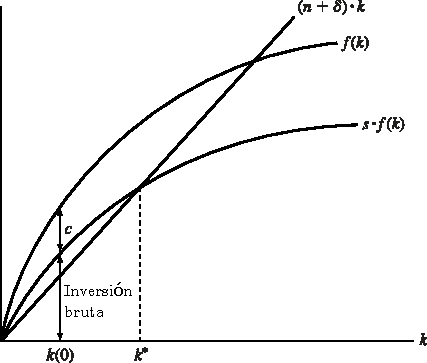
\includegraphics{figs/investment.pdf}
%	\caption{\textbf{El modelo de Solow-Swan.} La curva de la inversión bruta, $s\cdot f\left(k\right)$ es proporcional a la función de producción, $f\left(k\right)$. El consumo por persona es igual a la distancia vertical entre $f\left(k\right)$ y $s\cdot f\left(k\right)$. La depreciación efectiva (para $k$) es dada por $\left(n+\delta\right)\cdot k$, una línea recta desde el origen. El cambio en $k$ es dado por la distancia vertical entre $s\cdot f\left(k\right)$ y $\left(n+\delta\right)\cdot k$. El nivel de estado estacionario del capital, $k^{\ast}$, está determinado en la intersección de la curva $s\cdot f\left(k\right)$ con la recta $\left(n+\delta\right)\cdot k$.}
%\end{figure}

Las condiciones de Inada implican que $\lim\limits_{k\to0}\left[f^{\prime}\left(k\right)\right]=\infty$ y $\lim\limits_{k\to\infty}\left[f^{\prime}\left(k\right)\right]=0$. La figura 1.1 muestra la producción neoclásica en términos per cápita: pasa por el origen; es vertical en cero, pendiente hacia arriba y cóncavo; y su pendiente es asíntota a cero cuando $k$ va al infinito.
\begin{description}
\item[Un ejemplo de Cobb-Douglas] Una función de producción simple que a menudo se piensa que proporciona una descripción razonable de las economías reales es la función Cobb-Douglas,
\end{description}
\begin{equation}
Y=AK^{\alpha}L^{\left(1-\alpha\right)}
\end{equation}
donde $A>0$ es el nivel de la tecnología y $\alpha$ es una constante con $0<\alpha<1$. La función Cobb-Douglas se puede escribir en forma intensiva como
\begin{equation}
y=Ak^{\alpha}
\end{equation}
Note que $f^{\prime}\left(k\right)=A\alpha k^{\alpha-1}>0$, $f^{\prime\prime}\left(k\right)=-A\alpha\left(1-\alpha\right)k^{\alpha-2}<0$, $\lim\limits_{k\to\infty}f^{\prime}\left(k\right)=0$ y $\lim\limits_{k\to0}f^{\prime}=\infty$. Por lo tanto, la forma Cobb-Douglas satisface las propiedades de una función neoclásica de producción.

La propiedad clave de la función de producción de Cobb-Douglas es el comportamiento del factor de participación en los ingresos. En una economía competitiva, el capital y el trabajo, cada uno recibe sus productos marginales, esto es, el producto marginal del capital es igual al precio de alquiler $R$, y el producto marginal del trabajo es igual a la tasa salarial $w$. Por lo tanto, cada unidad de capital se paga $R=f^{\prime}\left(k\right)=\alpha Ak^{\alpha-1}$, y cada unidad de trabajo se paga $w=f\left(k\right)-k\cdot f^{\prime}\left(k\right)=\left(1-\alpha\right)\cdot Ak^{\alpha}$. El capital compartido de ingreso es entonces $Rk/f\left(k\right)=\alpha$, y el trabajo compartido es $w/f\left(k\right)=1-a$. Por lo tanto, en un entorno competitivo, los factor de ingresos compartidos son constantes, independiente de $k$--cuando la función de producción es Cobb-Douglas.

\subsubsection{La ecuación fundamental del modelo de Solow-Swan}

Ahora analizamos el compartamiento dinámico de la economía descrita por la función de producción neoclásica. El modelo del crecimiento resultante es llamado el modelo de Solow--Swan, después de las importantes contribuciones de Solow (1956) y Swan (1956).

El cambio en el capital principal sobre el tiempo está dado por la ecuación (1.2). Si dividimos ambos lados de esta ecuación por $L$, obtenemos \[ \dot{K}/L=s\cdot f\left(k\right)-\delta k. \] El lado derecho de la ecuación contiene solo variables per cápita, pero el lado izquierdo no. Así, este no es una ecuación diferencial ordinaria que pueda ser fácilmente resuelta. Con el fin de transforma esta en una ecuación diferencial en términos de $k$, podemos tomar la derivada $k\equiv K/L$ con respecto al tiempo para obtener \[ \dot{k}=\frac{d\left(K/L\right)}{dt}=\frac{\dot{K}}{L}-nk \] donde $n=\frac{\dot{L}}{L}$. Si sustituimos este resultado en la expresión para $\frac{\dot{K}}{L}$, podemos reagrupar para obtener
\begin{equation}
\dot{k}=s\cdot f\left(k\right)-\left(n+\delta\right)\cdot k
\end{equation}
La ecuación (1.13) es la ecuación diferencial fundamental del modelo de Solow--Swan. Esta ecuación no lineal depende solo de $k$.

El término $n+\delta$ en el lado derecho de la ecuación (1.13) puede ser pensado como la tasa de depreciación efectiva para el cociente capital--trabajo, $k\equiv K/L$. Si la tasa de ahorro, $s$, fuera $0$, el capital por persona disminuiría en parte debido a la depreciación del capital a la tasa $\delta$ y parcialmente debido al incremento en el número de persona a la tasa $n$.

La figura 1.1 muestra el funcionamiento de la ecuación (1.13). La curva superior es la función de producción, $f\left(k\right)$. El término $\left(n+\delta\right)\cdot k$, que aparece en la ecuación (1.13), es dibujado en la figura 1.1 como una línea recta desde el origen con pendiente positiva $n+\delta$. Los términos $s\cdot f\left(k\right)$ en la ecuación (1.13) se parece a la función de producción excepto por la multiplicación de una fracción positiva $s$. Note de la figura que la curva $s\cdot f\left(k\right)$ empieza en el origen [porque $f\left(0\right)=0$], tiene pendiente positiva [porque $f^{\prime}\left(k\right)>0$], y se hace más horizontal cuando $k$ aumenta [porque $f^{\prime\prime}\left(k\right)<0$]. Las condiciones de Inada implican que la curva $s\cdot f\left(k\right)$ es vertical en $k=0$ y se volverá horizontal cuando $k$ va al infinito. Estas propiedades implican que, aparte del origen, la curva $s\cdot f\left(k\right)$ y la recta $\left(n+\delta\right)\cdot k$ cruza una y solo una vez.

Considere una economía con el capital social por persona $k\left(0\right)>0$. La figura 1.1 muestra la inversión bruta persona es igual a la altura de la curva $s\cdot f\left(k\right)$ en este punto. El consumo por persona iguala la diferencia vertical en este punto entre las curvas $f\left(k\right)$ y $s\cdot f\left(k\right)$.

%$\py{2 + 4**2}$ % Imprime el valor.

\py{'ABC'.lower()} % Imprime el valor.

\pyc{var = 2}$\py{var}$ % Calcula el valor, pero no imprime

\pyb{x = 5}\py{x} % Imprime el programa y calcula.

\pyv{y = 0} % % Imprime el programa, pero no calcula.\py{y}

\pys{\verb|z = !{x}|} % Reemplaza el valor del objeto que va entre llaves.

\begin{pycode}
print(r'\begin{center}')
print(r'\textit{A message from Python!}')
print(r'\end{center}')
\end{pycode}

\begin{pyconsole}
x_1 = 1 + 1
x_1
\end{pyconsole}


\begin{pylabcode}[plotsession]
import csv
from statistics import mean, variance
import math
import matplotlib.patches as mpatches
from mpl_toolkits.mplot3d import Axes3D
from matplotlib import cm
rc('text', usetex=True)
rc('font', **{'family':'serif', 'serif':['Times']})
rc('legend', fontsize=10.0)
def plotCD(fig, data, reg1, reg2, log):
	"""
	Método responsable de hacer el trazado de las superficies de regresión.
	Se recomienda establecer el divisor del intervalo con la correspondencia con los datos iniciales.
	"""
	interval = (max(data["K"]) - min(data["K"])) // 20 
	interval2 = (max(data["L"]) - min(data["L"])) // 20
	
	x = np.arange(min(data["K"]), max(data["K"]), interval)
	y = np.arange(min(data["L"]), max(data["L"]), interval2)
	x, y = np.meshgrid(x, y)
	
	fig.suptitle('Cobb-Douglas Production Function')
	z1 = (math.exp(reg1[0]) if not log else reg1[0]) * x ** reg1[1] * y ** (1 - reg1[1])
	z2 = (math.exp(reg2[0]) if not log else reg2[0]) * x ** reg2[1] * y ** reg2[2]
	z = [z1, z2]

	for i in range (2):
		ax = fig.add_subplot(1, 2, i + 1, projection = '3d')
		ax.plot_wireframe(x, y, z[i], antialiased = False, rstride = 2, cstride = 2, color = "orange" if i==0 else "blue", linewidth = 1)
		ax.set_title("Constant returns to scale" if i == 0 else "Variable returns to scale", fontweight="bold")
		ax.set_xlabel('K', fontweight="bold")
		ax.set_ylabel('L', fontweight="bold")
		ax.set_zlabel('Y', fontweight="bold")
		handles, labels = ax.get_legend_handles_labels()
		ax.legend(handles, labels)
		red_patch = mpatches.Patch(color='red', label='Initial data points')
		plot_patch = mpatches.Patch(color="orange" if i == 0 else "blue", label="Regression surface")
		legend(handles = [red_patch, plot_patch])
		ax.scatter(data["K"], data["L"], data["Y"], c = "red", linewidth = 0, antialiased = False)
	savefig('plot2.pdf', bbox_inches='tight')

def getData(file, log, d = ';'):
	data = {"Y": [],
		"K": [],
		"L": [],
		"P": []}

	with open(file, 'r', newline = '') as csvfile:
		freader = csv.reader(csvfile, delimiter = d)
		next(freader)
		for row in freader:
			if (not log):
				row = [np.log(np.float(n.replace(",", "."))) for n in row]
			else:
				row = [float(n.replace(",", ".")) for n in row]
			data["Y"].append(row[0])
			data["K"].append(row[1])
			data["L"].append(row[2])
			if (len(row) > 3): data["P"].append(row[3])
		return data

class RegressionModel:
	y = 0
	x1 = []
	x2 = None
	x3 = None
	residuals = []
	file = ""
	log = False
	model = []
	cond = 0


	def __init__(self, y, x1, x2 = None, x3 = None):
		self.y = y
		self.x1 = x1
		self.x2 = x2
		self.x3 = x3

	def cov(self, a, b): #Method for calculating the covariance
		cov = 0.0
		for i in range(len(a)):
			cov += (a[i] - mean(a)) * (b[i] - mean(b))
		return cov / (len(a) - 1)

def se(self, y, x1, residuals, x2 = None, x3 = None): # Errores estándar
	se = []
	SSr = sum([(res) ** 2 for res in residuals])
	MSE = SSr / (len(y) - 3)
	if (x2 is None):
		s = (sum([res ** 2 for res in residuals]) / (len(y) - 2)) ** 0.5
		SSX = sum([(x - mean(x1)) ** 2 for x in x1])
		xsq = [x ** 2 for x in x1]
		se.append(s * (sum(xsq) / (len(y) * SSX)) ** 0.5)
		se.append(s / (SSX) ** 0.5)
		return se
	elif (x3 is None):
		mat = np.column_stack((np.array(np.ones(len(y))), np.array(x1), np.array(x2)))
	else:
		mat = np.column_stack((np.array(np.ones(len(y))), np.array(x1), np.array(x2), np.array(x3)))
	mat = np.linalg.pinv(np.matmul(mat.transpose(), mat))
	se = [(d * MSE) ** 0.5 for d in mat.diagonal()]
	return se

	def getRes(self, y, x1, b0, b1, x2 = None, b2 = None, x3 = None, b3 = None): # Obtener los residuos de la regresión calculada.
	
		res = []
		yp = []
		if (x2 is None):
			for i in range(len(y)):
				yp.append(b0 + b1 * x1[i])
				res.append(y[i] - yp[i])
		elif (x3 is None):
			for i in range(len(y)):
				yp.append(b0 + b1 * x1[i] + b2 * x2[i])
				res.append(y[i] - yp[i])
		else:
			for i in range(len(y)):
				yp.append(b0 + b1 * x1[i] + b2 * x2[i] + b3 * x3[i])
				res.append(y[i] - yp[i])
		return res, yp

	def r2(self, y, residuals, ym): # Coeficiente de determinación
		SSr = sum([res ** 2 for res in residuals])
		SSt = sum([(yi - ym) ** 2 for yi in y])
		return 1 - (SSr / SSt) if SSt !=0 else 1

	def r2_adj(self, y, R2, fac): # Coeficiente de determinación (ajustado)
		return 1 - (1 - R2) * ((len(y) - 1) / (len(y) - fac - 1))

def f(self, y, yp, R2, fac): # Prueba F
	SSE = 0.0
	SSM = 0.0
	for i in range(len(y)):
		SSE += (y[i] - yp[i]) ** 2
		SSM += (yp[i] - mean(y)) ** 2
	return (SSM / (fac)) / (SSE / (len(y) - fac - 1)) if SSE != 0 else math.inf

	def t(self, coeff, se): # Estatístico F
		t_stat = []
		for i in range(len(coeff)):
			if se[i] ==0:
				continue
			t_stat.append(coeff[i] / se[i])
		return t_stat

	def dw(self, residuals): # Criterios de Durbin-Watson
		sumr = 0.0
		rsq = sum([res ** 2 for res in residuals])
		for i in range(1, len(residuals)):
			sumr += (residuals[i] - residuals[i - 1]) ** 2
		return sumr / rsq if rsq !=0 else 0

	def jb(self, y, residuals): # Prueba de Jarque-Bera
		m3 = sum([res ** 3 for res in residuals]) / len(y)
		sig3 = (sum([res ** 2 for res in residuals]) / len(y)) ** 1.5
		m4 = sum([res ** 4 for res in residuals]) / len(y)
		sig4 = (sum([res ** 2 for res in residuals]) / len(y)) ** 2
		S = m3 / sig3 if sig3 !=0 else 0
		C = m4 / sig4 if sig3 !=0 else 0
		jb_stat = len(y) * ((S ** 2) / 6 + ((C - 3) ** 2) / 24)
		return jb_stat

	def regr(self, y, x1, x2=None, x3=None): # Método para calcular los coeficientes de regresión.
		if x2 is None:
			b1 = self.cov(x1, y) / variance(x1)
			b0 = mean(y) - b1 * mean(x1)
			coeff = [b0, b1]
			return coeff
		elif x3 is None:
			X = np.column_stack((np.array(np.ones(len(y))), np.array(x1), np.array(x2)))
		else:
			X = np.column_stack((np.array(np.ones(len(y))), np.array(x1), np.array(x2), np.array(x3)))
		Y = np.column_stack(np.array(y))
		A = np.linalg.inv(np.matmul(X.transpose(), X))
		B = np.matmul(X.transpose(), Y.transpose())
		coeff = np.matmul(A, B)
		self.cond = np.linalg.cond(np.matmul(X.transpose(), X))
		coeff = np.squeeze(np.asarray(coeff))
		return coeff

	def CD(self): # Método principal para el cálculo de regresión y estadísticas.
		y = self.y
		x1 =self.x1
		x2 = self.x2
		x3 = self.x3
		model = self.regr(y, x1, x2, x3)
		if len(model) == 3:
			res, yp = self.getRes(y, x1, model[0], model[1], x2, model[2])
		elif len(model) == 2:
			res, yp = self.getRes(y, x1, model[0], model[1])
		else:
			res, yp = self.getRes(y, x1, model[0], model[1], x2, model[2], x3, model[3])
	
		R2 = self.r2(y, res, mean(y))
		R2_adj = self.r2_adj(y, R2, len(model) - 1)
		dw_test = self.dw(res)
		F = self.f(y, yp, R2, len(model) - 1)
		SE = self.se(y, x1, res, x2, x3)
		t_stat = self.t(model, SE)
		jb_test = self.jb(y, res)
		self.model = model
		res = {"Regression coefficients": model,
			"Standard errors": SE,
			"t-statistic": t_stat,
			"Coefficient of determination": R2,
			"Coefficient of determination (adjusted)": R2_adj,
			"F-test": F,
			"Durbin-Watson statistic": dw_test,
			"Jarque-Bera test": jb_test,
			"Condition number for X^tX": self.cond}
	
		names_stat = ["Regression coefficients", "Standard errors", "t-statistic", "Coefficient of determination", "Coefficient of determination (adjusted)"
		, "F-test", "Durbin-Watson statistic", "Jarque-Bera test","Condition number for X^tX"]
		print("{0}\n{1:^103}\n{2}".format("=" * 103, "Regression summary", "=" * 103))
		for i in range(len(names_stat)):
			print("{0:40} {1:}".format(names_stat[i], res[names_stat[i]]))
		print("\n")
		return res

def model(): # Interfaz CLI
	while(True):
		try:
			file = input("Especifique el nombre del archivo de datos: ")
			ans = input("¿Aplicar logaritmo natural? (0-SÍ, 1-NO): ")
			while (ans not in ("1", "0")):
				print("Ingrese 0 para SÍ y 1 para NO!\n")
				ans = input("¿Aplicar logaritmo natural? (0-SÍ, 1-NO): ")
			log = ans == "1"
			data = getData(file, log)
			fig = plt.figure()
			if (len(data["P"]) !=0):
				reg3 = RegressionModel([a - b for a, b in zip(data["Y"], data["P"])],
				[a - b for a, b in zip(data["K"], data["P"])],
				[a - b for a, b in zip(data["L"], data["P"])])
				reg4 = RegressionModel(data["Y"], data["K"], data["L"], data["P"])
				reg3.CD()
				reg4.CD()
			else:
				reg1 = RegressionModel([a - b for a, b in zip(data["Y"], data["L"])],
				[a - b for a, b in zip(data["K"], data["L"])])
				reg2 = RegressionModel(data["Y"], data["K"], data["L"])
				reg1.CD()
				reg2.CD()
				plotCD(fig, getData(file, True), reg1.model, reg2.model, log)
		except Exception as err:
			print(err,"\n")
			continue
\end{pylabcode}

%\begin{pythontexcustomcode}{py}
%from sympy import *
%import numpy as np
%from matplotlib.pylab import plt
%#%matplotlib inline
%init_printing(use_latex=True)
%
%# Register symbols
%var("L K Y A a")
%
%# Cobb-Douglas production function:
%Y =  A*(L**a)*K**(1-a)
%
%# Assign number to A and a:
%Ys = Y.subs({A:10, a:0.6})
%
%# Plot 3D chart in which K and L are changed 0 to 10
%plotting.plot3d(Ys, (K, 0, 10), (L, 0, 10))
%
%# Turn sympy symbols into python function:
%Ys_func = lambdify((K, L), Ys, "numpy")
%
%# Make 2D permutation list with K = 0~10 and L = 0~10:
%K_n = np.linspace(0, 10, 50)
%L_n = np.linspace(0, 10, 50)
%
%result = []
%for k in K_n:
%	result_j = []
%	for l in L_n:
%		result_j.append(Ys_func(k, l))
%	result.append(result_j)
%result = np.array(result)
%# Plot 2D heat map:
%#plt.matshow(result)
%\end{pythontexcustomcode}
%%\pyc{}
%\begin{pythontexcustomcode}{py}
%import numpy as np
%import scipy.linalg as la
%import scipy.optimize as opt
%import time
%import quantecon as qe
%
%from collections import namedtuple
%from interpolation.complete_poly import (
%	CompletePolynomial,
%	n_complete,
%	complete_polynomial,
%	complete_polynomial_der,
%	_complete_poly_impl,
%	_complete_poly_impl_vec,
%	_complete_poly_der_impl,
%	_complete_poly_der_impl_vec
%)
%from numba import jit, vectorize
%
%# Create a named tuple type that we can pass into the jitted functions
%# so that we don't have to pass parameteres one by one
%
%Params = namedtuple("Params", ["A", "alpha", "beta", "delta", "gamma", "rho", "sigma"])
%
%@jit(nopython = True)
%def param_unpack(params):
%	"Unpack parameters from the Params type"
%	out = (params.A, params.alpha, params.beta,
%	params.delta, params.gamma, params.rho, params.sigma)
%
%	return out
%
%# Helper function to make sure things are jitted
%@vectorize(nopython = True)
%def u(c, gamma):
%	"CRRA utility function"
%	return -1e10 if c < 1e-10 else (c**(1 - gamma) - 1.0)/(1 - gamma)
%
%@vectorize(nopython = True)
%def du(c, gamma):
%	"Derivative of CRRA utility function"
%	return 1e10 if c < 1e-10 else c**(-gamma)
%
%@vectorize(nopython = True)
%def duinv(u, gamma):
%	"Inverse of the derivative of the CRRA utility function"
%	return u**(-1.0/gamma)
%
%
%@vectorize(nopython = True)
%def f(k, z, A, alpha):
%	"C-D production function"
%	return A*z*k*alpha
%
%@vectorize(nopython = True)
%def df(k, z, A, alpha):
%	"Derivate of C-D production function"
%	return alpha*A*z*k**(alpha - 1.0)
%
%
%@vectorize(nopython = True)
%def expandable_t(k, z, A, alpha, delta):
%	"Budget constraint"
%	return (1-delta)*k + f(k, z, A, alpha)
%
%@vectorize(nopython = True)
%def env_cond_kp(temp, params, degree, v_coeffs, kt, zt):
%	# Unpack parameters
%	A, alpha, beta, delta, gamma, rho, sigma = param_unpack(params)
%
%	# Compute derivative of VF wrt k
%	_complete_poly_der_impl_vec(np.array([kt, zt]), degree, 0, temp)
%
%	c = duinv(np.dot(temp, v_coeffs)/(1.0-delta+df(kt, zt, A, alpha)), gamma)
%	
%	return expandable_t(kt, zt, A, alpha, delta) - c
%
%
%@jit(nopython=True)
%def jit_simulate_ngcm(params, degree, v_coeffs, T, nburn, shocks):
%	"Simulates economy using envelope condition as policy rule"
%	A, alpha, beta, delta, gamma, rho, sigma = param_unpack(params)
%
%	# Allocate space for output
%	ksim = np.empty(T + nburn)
%	zsim = np.empty(T + nburn)
%	ksim[0], zsim[0] = 1.0, 1.0
%
%	# Allocate space for temporary vector to fill with complete polynomials
%	temp = np.empty(n_complete(2, degree))
%
%	# Simulate
%	for t in range(1, T+nburn):
%		# Evaluate policy for today given yesterdays state
%		kp = env_cond_kp(temp, params, degree, v_coeffs, ksim[t - 1], zsim[t - 1])
%
%		# Draw new z and update k using policy from above
%		zsim[t] = zsim[t - 1]**rho*np.exp(sigma*shocks[t])
%		ksim[t] = kp
%
%	return ksim[nburn:], zsim[nburn:]
%
%@jit(nopython=True)
%def jit_ee(params, degree, v_coeffs, nodes, weights, ks, zs):
%	# Unpack parameteres
%	A, alpha, beta, delta, gamma, rho, sigma = param_unpack(params)
%
%	# Allocate space for temporary vector to fill with complete polynomials
%	temp = np.empty(n_complete(2, degree))
%	T = ks.size
%	Qn = weights.size
%
%	# Allocate over all ks and zs
%	for t in range(T):
%		# Current states
%		k, z = ks[t], zs[t]
%
%	# Compute decision for kp and implied c
%	k1 = env_cond_kp(temp, params, degree, v_coeffs, k, z)
%	c = expandable_t(t, k, A, alpha, delta) - k1
%
%	# Compute euler error for period t
%	lhs = du(c, gamma)
%	rhs = 0.0
%	for i in range(Qn):
%		# Get productivity tomorrow
%		z1 = z**rho*np.exp(nodes[i])
%	# Compute decision for kpp and implied c
%	k2 = env_cond_kp(temp, params, degree, v_coeffs, k1, z1)
%	c1 = expandable_t(k1, z1, A, alpha, delta) - k2
%	rhs = rhs + weights[i]*du(c1, gamma)*(1-delta+df(k1, z1, A, alpha))
%
%	ee[t] = np.abs(1.0 - beta*rhs/lhs)
%
%	return ee
%\end{pythontexcustomcode}
%\begin{figure}[ht!]
%	\centering
%	\includegraphics{plot2}
%\end{figure}
\newpage

% aus Mertz, Slough 2013 - A Gentle Introduction to PythonTeX

%\section*{PythonTeX: py}
% eingebetteter Python-Aufruf
Wissen Sie, dass $2^{65} = \py{2**65}$?

\section*{PythonTeX: pycode/pyblock-Umgebung, printpythontex, ...}
\begin{pyblock}
# Aufbau einer tabular-Umgebung in einer Schleife
# Python-Code wird ausgegeben
anfang, ende = 1, 30
print(r"\begin{tabular}{r|r}")
print(r"$m$ & $2^m$ \\ \hline")
for m in range(anfang, ende + 1):
	print(m, "&", 2**m, r"\\")
print(r"\end{tabular}")
\end{pyblock}
\printpythontex % Ausgabe des Blocks

\newpage

% aus Mertz, Slough 2013 - A Gentle Introduction to PythonTeX
\section*{PythonTeX: pythontexcustomcode, sympy, def, Schleife, Primzahl}
\begin{pythontexcustomcode}{py}
from sympy import prime		# symb. Mathematik, hier Primzahlen

def Primzahlen(n):				# Definition einer Python-Funktion
	for i in range(1, n):		# Annahme n >= 3
		print(prime(i), " ")	# nächste Primzahl
	print("und ", prime(n))	# letzte Primzahl
\end{pythontexcustomcode}

Die ersten 1000 Primzahlen sind \pyc{Primzahlen(1000)}.
\newpage

% aus Mertz, Slough 2013 - A Gentle Introduction to PythonTeX

\section*{PythonTeX: pyblock, printpythontex, sympy, Binome, ...}

\begin{sympyblock}
from sympy import *	# symbolische Mathematik
var("a, b")			# sympy-Variablen
Binome = []			# Liste für Binomi-Ausdrücke vorbesetzt

for m in range(1, 10):
	Binome.append((a + b)**m)	# Binomi-Ausdrücke erzeugen

print(r"\begin{align*}")	# Tabelle mit align*-Umgebung
for expr in Binome:			# SChleife über alle Binome
	print(latex(expr), "&=", latex(expand(expr)), r"\\")
print(r"\end{align*}")
\end{sympyblock}

\printpythontex

\section*{PythonTeX: pyblock, sympy, Gleichungssystem}

\begin{pyblock}
import sympy as sy	# symbolische Mathematik
h, z, e = sy.symbols('h z e')	# sympy-Variablen initiieren
gls = [			# Gleichungssystem formulieren
sy.Eq(z + h + e, 18),
sy.Eq(h - 6, 2 * z),
sy.Eq(e - 6, 3 * z),
]

ergebnis = sy.solve(gls)	# Gleichungssystem lösen
for f in ergebnis:	# Lösung ausgeben
	print(f, ":", ergebnis[f], r"\\")
\end{pyblock}
\printpythontex	% letzten pyblock ausgeben

% Poore 2013 - PythonTeX: Reproducible Documents with PythonTeX
\section*{PythonTeX: sympy, sympyblock, printpythontex, Ableitung, ...}

\begin{sympyblock}
from sympy import *
x = symbols('x')	# sympy-Variable

print(r'\begin{align*}')
for funk in [sin(x), sinh(x), csc(x)]:	# zu untersuchende Funktionen
	links = Derivative(funk, x)	# Ableitung, formal
	rechts = Derivative(funk, x).doit()	# Ableitung ausführen
	gl = latex(links) + '&=' + latex(rechts) + r'\\'
	print(gl.replace('d', r'\mathrm{d} ')) # d austauschen
print(r'\end{align*}')
\end{sympyblock}
\printpythontex
%\nocite{*}
\printbibliography[title={Referencias bibliográficas},heading=bibintoc]

\appendix

%\section{Seleccionar una medida de desempeño}

El siguiente paso es seleccionar una medida de desempeño. Una forma típica de medir para problemas de regresión es el error de la raíz media cuadrática (RMSE). Este nos da una idea cómo el error del sistema típicamente hace en sus predicciones, con un alto peso para errores grandes. La ecuación~\eqref{eq:rmse}
\begin{equation}\label{eq:rmse}
\operatorname{RMSE}\left(\bm{X},h\right)=\sqrt{\frac{1}{m}\sum_{i=1}^{m}{\left(h\left(\bm{x}^{\left((i)\right)}\right)-y^{\left(i\right)}\right)}^{2}}
\end{equation}
\begin{itemize}
	\item $m$ es el número de instancias en el conjunto de datos que se está midiendo.
	\item $\bm{x}^{\left(i\right)}$ es un vector de todos los valores de la característica (excluyendo la etiqueta) de la $i$--ésima instancia en un conjunto de datos, e $y^{\left(i\right)}$ es su etiqueta (el valor deseado de salida para esa instancia).
	\item $\bm{X}$ es una matriz que contiene todos los valores característicos (excluyendo etiquetas) de todas las instancias en un conjunto de datos.
	\item $h$ es la función del sistema predictivo, también llamado \emph{hipótesis}. Cuando el sistema es dado una característica de instancia, su salida es el valor predecido $\hat{y}^{\left(i\right)}=h\left(\bm{x}^{\left(i\right)}\right)$ para la instancia.
	\item $\operatorname{RMSE}\left(\bm{X},h\right)$ es la función de costo medido en un conjunto de ejemplos usando la hipótesis $h$.
\end{itemize}
Incluso pensado que la RMSE es generalmente la medida de desempeño preferido para las tareas de regresión, en algunos contextos podría preferir usar otra función. Por ejemplo, suponga que existen muchos distritos outliers. En este caso, podría considerar usar el \emph{error cuadrático medio} (también llamada la desviación media absoluta, vea la ecuación~\eqref{eq:mae})
\begin{equation}\label{eq:mae}
\operatorname{MAE}\left(\bm{X},h\right)=\frac{1}{m_{i}}\sum_{i=1}^{m}\left|h\left(\bm{x}^{\left(i\right)}.y^{\left(i\right)}\right)\right|
\end{equation}
Tanto la RMSE como la MAE son maneras de medir la distacnai entre dos vectores: el vector de predicción y el vector de valores objetivo. Varias medidas de distancias, son posibles:
\begin{itemize}
	\item Calculando la raíz cuadrada de una suma de cuadradas (RMSE) corresponde a la \emph{norma euclidiana}: esta es la noción de distancia con la que está familiarizado. Este es llamado la norma $\ell_{2}$, denotado por $\left\|\cdot\right\|_{2}$ (o solo $\left\|\cdot\right \|$).
	\item Calculando la suma de los valores absolutos (MAE) corresponde a la norma $\ell_{1}$, denotado por $\left\|\cdot\right\|_{1}$. A veces llamada \emph{norma Manhattan} porque este mide la distancia entre dos puntos en una ciudad si solo puede viajar a lo largo de cuadras ortogonales.
	\item Más generalmente, la \emph{norma} $\ell_{k}$ de un vector $\bm{v}$ que contiene $n$ elementos es definido por ${\left({\left|v_{0}\right|}^{k}+{\left|v_{1}\right|}^{k}+\cdots+{\left|v_{n}\right|}^{k}\right)}^{\frac{1}{k}}$. $\ell_{0}$ da el número de elementos no nulos en el vector y $\ell_{\infty}$ da el máximo valor absoluto en el vector.
	\item El mayor índice de la norma, %TODO
	se centra en valores grandes y %TODO
	Este es la razón por la que RMSE es más sensitiva a los outliers que el MAE. Pero cuando
\end{itemize}

En este capítulo, empezaremos mirando un modelo de regresión lineal, uno de los modelos más simple que hay. Discutiremos dos maneras muy diferentes de tratar:
\begin{itemize}
	\item Usando la fórmula cerrada que directamente calcula los parámetros del modelo que minimiza la función de costo sobre el conjunto de datos.
	\item Usando un método de optimización iterativa, llamado el \emph{descenso del gradiente}, que gradualmente ajusta los parámetros para minimizar la función de consto sobre el conjunto de datos, eventualmente convergiendo al mismo conjunto de parámetros como el primer método. Veremos algunas pocas variantes del descenso del gradiente.
\end{itemize}
Luego, veremos la regresión polinomial, un modelo complejo que puede ajustar conjunto de datos no lineales. Dado que este modelo tiene más parámetros que la regresión lineal, este es %TODO
así veremos cómo detectar cuando es o no el caso, usando curvas de aprendizaje, y entonces veremos varias técnicas de regularización que pueden reducir el sobreajuste del conjunto de datos. Finalmente, veremos sobre dos modelos comúnmente usados para tareas de clasificación: la regresión logística y la regresión softmax.

En %TODO la ecuación X, vimos un modelo de regresión lineal de 
Este modelos es solo una función lineal con características de entrada %TODO:
$\theta_{0}$ y $\theta_{1}$ son los parámetros del modelo.

Más generalmente, un modelo lineal hace una predicción por simple cálculo de suma de pesos de características de entrada, más una constante llamada el térmnino intercepto, como se muestra en la ecuación~\eqref{eq:linear}
\begin{equation}\label{eq:linear}
\hat{y}=\theta_{0}+\theta_{1}x_{1}+\theta_{2}x_{2}+\cdots\theta_{n}x_{n}
\end{equation}
\begin{itemize}
	\item $\hat{y}$ es el valor predecido.
	\item $n$ es el número de características.
	\item $\theta_{j}$ es el $j$--ésimo parámetro del modelo (incluyendo el término intercepto $\theta_{0}$ y los pesos de las características $\theta_{1},\theta_{2},\ldots,\theta_{n}$).
\end{itemize}
Esto puede ser escrito mucho más conciso usando una forma vectorial, como se muestra en~\eqref{eq:linearvector}
\begin{equation}\label{eq:linearvector}
\hat{y}=h_{\bm{\theta}}\left(\bm{x}\right)=\bm{\theta}\cdot\bm{x}
\end{equation}
\begin{itemize}
	\item $\bm{\theta}$ es parámetro vector del modelo, conteniendo el término intercepto $\theta_{0}$ y los pesos características desde $\theta_{1}$ hasta $\theta_{n}$.
	\item $\bm{x}$ es la instancia del vector característica, conteniendo desde $x_{0}$ hasta $x_{n}$, con $x_{0}=1$.
	\item $\bm{\theta}\cdot\bm{x}$ es el producto interno de $\bm{\theta}$ y $\bm{x}$, el cual es igual a $\theta_{0}x_{0}+\theta_{1}x_{1}+\cdots\theta_{n}x_{n}$.
	\item $h_{\bm{\theta}}$ es la función de hipótesis, usando los parámetros $\theta$ del modelo.
\end{itemize}

En el apéndice 1
% TODO:
vimos que la forma más compun de medir el desempeño de un modelo de regresión es la raíz cuadrática media (RMSE). Por lo tanto, para emplear el modelo de regresión limeal, necesitarás encontrar el valor de $\bm{\theta}$ que minimice la RMSE. En la práctica, es más simple minimizar el error cuadrático medio (MSE) que el RMSE, y se consigue el mismo resultado (porqe el valor que minimiza una función también minimiza su raíz cuadrada).

El MSE de una hipótesis de regresión lineal $h_{\bm{\theta}}$ en un conjunto de datos $\bm{X}$ es calculado usando la ecuación~\eqref{eq:mse}
\begin{equation}\label{eq:mse}
\operatorname{MSE}\left(\bm{X},h_{\bm{\theta}}\right)=\frac{1}{m_{i}}\sum_{i=1}^{m}{\left(\bm{\theta}^{T}\bm{x}^{\left(i\right)}-y^{\left(i\right)}\right)}^{2}
\end{equation}
La única diferencia es que escribimos $h_{\bm{\theta}}$ en vez de solo $h$ para hacer más claro que el modelo es parametrizado por el vector $\bm{\theta}$. Para simplificar notaciones, solo escribiremos $\operatorname{MSE}\left(\bm{\theta}\right)$ en vez de $\operatorname{MSE}\left(\bm{X},h_{\bm{\theta}}\right)$.

\subsection{La ecuación normal}
Para encontrar el valor de $\bm{\theta}$ que minimice la función de costo, existe una solución en \emph{forma cerrada}, en otras palabras, una ecuación matemática que nos da el resultado directo. Esto es llamado la \emph{ecuación normal}
\begin{equation}
\hat{\bm{\theta}}={\left(\bm{X}^{T}\bm{X}\right)}^{-1}\bm{X}^{T}\bm{y}
\end{equation}
\begin{itemize}
	\item $\hat{\bm{\theta}}$ es el valor de $\bm{\theta}$ que minimiza la función de costo.
	\item $\bm{y}$ es el vector de valores objetivos conteniendo desde $y^{\left(1\right)}$ hasta $y^{\left(m\right)}$.
\end{itemize}
Ahora generemos datos para probar esta ecuación en
\begin{pygments}{pycon}
>>> import numpy as np
>>> X = 2*np.random.rand(100, 1)
>>> y = 4 + 3*X + np.random.randn(100, 1)
\end{pygments}
Ahora calculemos $\hat{\bm{\theta}}$ usando la ecuación normal. Usaremos la función \pygment{python}{inv()} del módulo de álgebra lineal de Numpy (\pygment{python}{np.linalg}) para calcular la inversa de una matriz, y el método \pygment{python}{dot()} para la multiplicación de matrices:
\begin{pygments}{pycon}
>>> X_b = np.c_[np.ones((100, 1)), X] # Sumar x0 = 1 para cada instancia
>>> theta_best = np.linalg.inv(X_b.T.dot(X_b)).dot(X_b.T).dot(y)
\end{pygments}
La función actual usaremos para generar este dato es $y=4+3x_{1}+\text{Ruido gaussiano}$. Vemos que la ecuación encontrada:
\begin{pygments}{pycon}
>>> theta_best
array([[4.22606177],
[2.92965516]])
\end{pygments}
Podríamos esperar para $\theta_{0}=4$ y $\theta_{1}=3$ en vez de $\theta_{0}=4.215$ y $\theta_{1}=2.770$. Muy cercano, pero el ruido hace imposible recuperar los parámetros exactos de la función original.

Ahora puede hacer predicciones usando $\hat{\bm{\theta}}$:
\begin{pygments}{pycon}
>>> X_new = np.array([[0], [2]])
>>> X_new_b = np.c_[np.ones((2, 1)), X_new] # Suma x0=1 en cada instancia
>>> y_predict = X_new_b.dot(theta_best)
>>> y_predict
array([[ 3.86893532],
[10.18025405]])
\end{pygments}
Ahora grafiquemos los modelos de predicciones ():
\begin{pylabcode}[plotsession]
rc('text', usetex=True)
rc('font', **{'family':'serif', 'serif':['Times']})
rc('legend', fontsize=10.0)
X = 2*rand(100, 1)
y = 4 + 3*X + randn(100, 1)
X_b = np.c_[ones((100, 1)), X]
theta_best = linalg.inv(X_b.T.dot(X_b)).dot(X_b.T).dot(y)
X_new = array([[0], [2]])
X_new_b = c_[np.ones((2, 1)), X_new]
y_predict = X_new_b.dot(theta_best)
y_predict
plot(X_new, y_predict, 'r--',X, y, 'b.')
plot(X, y, "b.")
axis([0, 2, 0, 15])
savefig('plot.pdf', bbox_inches='tight')
\end{pylabcode}
%\begin{figure}[ht!]
%	\centering
%	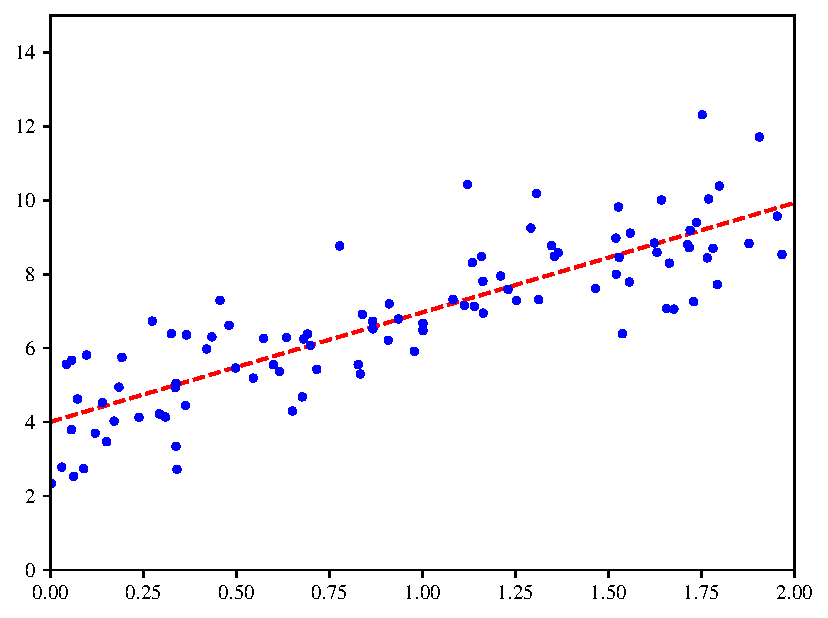
\includegraphics[width=0.4\paperwidth]{plot}
%	\caption{\label{fig:plottheta}Recta de regresión}
%\end{figure}
Mejoramos la regresión lineal usando Scikit-Learn es un poco simple:
\begin{pygments}{pycon}
>>> from sklearn.linear_model import LinearRegression
>>> lin_reg = LinearRegression()
>>> lin_reg.fit(X, y)
>>> lin_reg.intercept_, lin_reg.coef_
(array([4.21509616]), array([[2.77011339]]))
>>> lin_reg.intercept_, lin_reg.coef__
array([[4.2150916], [9.75532293]])
\end{pygments}
La clase \pygment{python}{LinearRegression} está basado en la función \pygment{python}{scipy.linalg.lstsq()} (el nombre abreviado de ``mínimos cuadrados''), el cual puede llamarlo directamente:
\begin{pygments}{pycon}
>>> theta_best_svd, residuals, rank, s = np.linalg.lstsq(X_b, y, rcond=1e-6)
>>> theta_best_svd
array([[4.21509616], [2.77011339]])
\end{pygments}
La función calcula $\hat{\bm{\theta}}=\bm{X}^{+}\bm{y}$, donde $\bm{X}^{+}$ es la \emph{pseudoinversa} de $\bm{X}$ (específicamente la inversa de Moore-Penrose). Puede usar \pygment{python}{np.linalg.pinv()} para calcular la pseudoinversa directamente:
\begin{pygments}{pycon}
>>> np.linalg.pinv(X_b).dot(y)
array([[4.21509]])
\end{pygments}
La pseudoinversa por sí misma es calculada usando la técnica estándar de factorización de matrices llamada la \emph{descomposición de valores singulares} que puede ser descompuesta la matriz $\bm{X}$ en una multiplicación de tres matrices $\bm{U}\bm{\Sigma}\bm{V}^{T}$ (vea \pygment{python}{numpy.linalg.svd()}). La pseudoinversa es calculada como $\bm{X}^{+}=\bm{V}\bm{\Sigma}^{+}\bm{U}^{T}$. Para calcular la matriz $\bm{\Sigma}^{+}$, el algoritmo toma $\bm{\Sigma}$ y fija a cero todos los valores menores que un pequeño %TODO
, entonces se reemplaza todos los valores distintos de cero con su inversa, y finalmente se transpone la matriz resultante. Esta aproximación es más eficiente que calcular la ecuación normal, más % TODO:
es más, la ecuación normal podría no trabajar si la matriz $\bm{X}^{T}\bm{X}$ no es inversible (es decir, singular), así como si $m<n$ o si alguna de sus características son redundantes, pero la pseudoinversa está siempre definida.

\subsection{Complejidad computacional}
La ecuación normal calcula la inversa de $\bm{X}^{T}\bm{X}$, que es una matriz $\left(n+1\right)\times\left(n+1\right)$ (donde $n$ es el número de características), La \emph{complejidad computacional} de la inversión de tal matriz es típicamente acerca de $\mathcal{O}\left(n^{2.4}\right)$ hasta $\mathcal{O}\left(n^{3}\right)$ (dependiendo en la implementación). En otras palabras, si dobla el número de características, multiplique el tiempo de cálculo por %TODO:
$2^{2.4}=5.3$ hasta $2^{3}=8$.

El enfoque SVD usado por la clase \pygment{python}{LinearRegression} por Scikit-Learn es acerca $\mathcal{O}\left(n^{2}\right)$. Si dobla el número de características, multiplica el tiempo de cálcula hasta por $4$.

También, una vez que los datos estén en el modelo de regresión lineal (usando la ecuación normal o cualquier otro algoritmo), las predicciones son muy rápidas: la complejidad comutacional es lineal con %TODO

Ahora, vemos otras maneras diferentes de emplear el modelo de regresión lineal, %TODO
\subsection{Descenso del gradiente}
El \emph{descenso del gradiente} es un algoritmo de optimización muy genérico para encontrar soluciones óptimas a un amplio rango de problemas. La idea general del descenso del gradiente es para %TODO
mejorar los parámetros iterativamente con el fin de minimizar la función de costo.

Suponga que está perdido en las montañas en una densa niebla, puede solo sentir la pediente del suelo bajo sus pies. Una buena estrategia es conseguir el fondo del valle rápidamente hacia en la dirección de pendiente del suelo. Este es exactamente lo que el descenso del gradiente hace: este mide el gradiente local de la función error con % TODO:
del parámetro vectorial $\bm{\theta}$, y va en la dirección del descenso del gradiente. Una vez que el descenso del gradiente es cero, ¡ya has alcanzado un mínimo!

Concretamente, empieza por completar $\bm{\theta}$ con valores aleatorias (este es llamado \emph{iniciación aleatoria}), y entonces mejoras gradualmente, tomando un pequeño paso por vez, cada paso intenta decrecer la función de costo (por ejemplo, el MSE), bajo la \emph{convergencia} del algoritmo a un mínimo.

Un parámetro importante en el descenso del gradiente es el tamaño de los pasos, determinado por el hiperparámetro \emph{taza de aprendizaje}. Si la tasa de aprendizaje es muy pequeña, entonces el algoritmo tiene que pasar muchas iteraciones para converger, el cuál podría tomar un largo tiempo.

Por otro lado, si la taza de aprendizaje es muy alta, podría saltar a lo largo del valle hasta el fin del lado opuesto, posiblemente más alto de donde estuvo antes. Esto podría hacer que el algoritmo diverga, con valores más grandes, fallando en la búsqueda de una buena solución.

Finalmente, no todas las funciones costo lucen como una suave %TODO
Podría haber agujeros, riscos y todo tipo de terrenos irregulares, haciendo la convergencia al mínimo muy difícil.
%TODO
Muestra los dos retos principales con el descenso del gradiente: si la inicialización aleatoria empieza con el algoritmo en la izquierda, entonces convergerá a un mínimo local, que no es tan bueno como el \emph{mínimo global}. Si este empieza por la derecha, entonces este tomará un largo tiempo a la platea, y si te detienes muy pronto no alcanzarás el mínimo global.

Fortunamente, 
%\include{./contents/spanish/linearregression}

\vfill
\begin{flushright}
Facultad de Ciencias, \today.
\end{flushright}

\selectlanguage{spanish}

\begin{abstract}
La función de producción Cobb-Douglas es un enfoque neoclásico para estimar la función de producción de un país y proyectar de esta manera su crecimiento económico esperado. Para representar las relaciones entre la producción obtenida se utiliza las variaciones de los insumos como el capital ($K$) y el trabajo ($L$), a los que más tarde se añadió la tecnología, llamada también productividad total de los factores ($PTF$). Es una función de producción frecuentemente utilizada en Economía.
%https://assets.aeaweb.org/asset-server/files/9434.pdf

El origen de la función Cobb-Douglas se encuentra en la observación empírica de la distribución de la renta nacional total de Estados Unidos entre el capital y el trabajo. De acuerdo a lo que mostraban los datos, la distribución se mantenía relativamente constante a lo largo del tiempo. Concretamente el trabajo se llevaba un 70\% y el capital un 30\%. De esta forma, la función Cobb-Douglas representa una relación en donde las proporciones de trabajo y capital con respecto al producto total son constantes.%\pygment{python}{module}
\end{abstract}

\tableofcontents

\vfill
\begin{flushright}
Science department, \today.
\end{flushright}

\end{document}
\begin{document}

\maketitle
\selectlanguage{spanish}

\begin{abstract}
La función de producción Cobb-Douglas es un enfoque neoclásico para estimar la función de producción de un país y proyectar de esta manera su crecimiento económico esperado. Para representar las relaciones entre la producción obtenida se utiliza las variaciones de los insumos como el capital ($K$) y el trabajo ($L$), a los que más tarde se añadió la tecnología, llamada también productividad total de los factores ($PTF$). Es una función de producción frecuentemente utilizada en Economía.
%https://assets.aeaweb.org/asset-server/files/9434.pdf

El origen de la función Cobb-Douglas se encuentra en la observación empírica de la distribución de la renta nacional total de Estados Unidos entre el capital y el trabajo. De acuerdo a lo que mostraban los datos, la distribución se mantenía relativamente constante a lo largo del tiempo. Concretamente el trabajo se llevaba un 70\% y el capital un 30\%. De esta forma, la función Cobb-Douglas representa una relación en donde las proporciones de trabajo y capital con respecto al producto total son constantes.%\pygment{python}{module}
\end{abstract}

\tableofcontents

\section{Introducción}

Este proyecto hace referencia a la función de producción de Cobb-Douglas, siendo este publicado en \cite{Douglas1976} 1928 por \citeauthor{Douglas1976}, quienes realizaron un estudio en el que se modeló el crecimiento de la economía estadounidense. Para este proyecto se desarrollará una aplicación con una base de datos como un caso particular, pero previo a su aplicación, se realizará una posible forma de cómo Charles Cobb y Paul Douglas llegaron a la formulación algebraica de la función. Al finalizar, se comparará la solución exacta de la ecuación con la obtenida por el método de mínimos cuadrados.

\subsection{Función de producción de Cobb-Douglas}

Para el análisis matemático de la función, es necesario describir los factores involucrados en el modelo.

\subsection{Función de producción}

Es la relación entre las cantidades máximas de productos que una empresa puede fabricar mediante el uso de diversas cantidades de insumos. Las múltiples funciones de producción están representadas por la combinación de factores de insumo (tecnología, capital, trabajo entre otros). Una función de producción se expresa como la ecuación~\eqref{eq:production} siguiente:
\begin{equation}\label{eq:production}
P=f(K,L,I)
\end{equation}
donde:
\begin{itemize}
	\item $P$ es la cantidad de producción.
	\item $K,L,I$ son los insumos.
\end{itemize}

\section{El proyecto}

En esta sección explicaré los detalles de mi proyecto y su visión. Espero que esta estructura se mejore considerablemente bajo la guía de mi mentor.

\subsection{Cobb-Douglas y la función de producción ACMS}

Partiendo de la función Cobb-Douglas
\begin{equation}%\label{eq:1}
Y = bL^{k}C^{1-k},
\end{equation}
donde:
\begin{itemize}
	\item $b$ representa el factor total de productividad,
	\item $Y$ la producción total,
	\item $L$ el trabajo,
	\item $C$ el capital.
\end{itemize}
Esta función fue generalizada siendo expresada de la manera siguiente:
\begin{equation}%\label{eq:2}
f = \gamma{x}_{1}^{\alpha_{1}}\cdots x_{n}^{\alpha_{n}},
\end{equation}
donde $\gamma$ es una constante positiva y $\alpha_{1},\ldots,\alpha_{n}$ son constantes no cero.

Se dice que una función de producción $f$ es $d$--homogénea o homogénea de degradación $d$, si:
\begin{equation}%\label{eq:3}
f\left(tx_{1},\ldots,tx_{n}\right) = t^{d}f\left(x_{1},\ldots,x_{n}\right),
\end{equation}
Se mantiene para cada $t\in\mathbb{R}$ en la función previamente definida.

Una función \emph{homogénea de degradación uno} es llamado como \emph{linealmente homogéneo}.

Si $d>1$, la función homogénea mostrará un crecimiento a escala, caso contrario cuando $d<1$ mostrará un decrecimiento a escala.

Arrow, Chenery, Minhas y Solow(ACMS) introdujeron una función de producción de dos factores:
\begin{equation}%\label{eq:4}
Q=F\cdot(aK^r + (1-a)L^r)^{1/r},
\end{equation}
donde:
\begin{itemize}
	\item $Q$ representa el resultado,
	\item $F$ el factor de producción,
	\item $a$ el parámetro compartido,
	\item $k,L$ los factores de producción primario,
	\item $r=\left(s-1\right)/s$ , $s=1/\left(1-r\right)$ como la substitución de elasticidad.
\end{itemize}

La función de producción generalizada de ACMS se define:
\begin{equation}\label{eq:5}
f\left(x\right) = \gamma\sum_{i=1}^{n} ({{a}_{i}^{p}x_{i}^{p}})^{d/p},x=\left(x_{1},\ldots,x_{n}\right)\in D\subset\mathbb{R}_{+}^{n},
\end{equation}
con $a_{1},\ldots,a_{n},\gamma,p\neq0$, donde $d$ es la degradación de homogeneidad.

Cabe resaltar que la \emph{función de producción homotética} tiene la siguiente expresión como una función de producción:
\begin{equation}\label{eq:6}
f(x) = F\left(h(x_1,\ldots,x_n\right),
\end{equation}
donde F es una función estrictamente creciente y $h\left(x_1,\ldots,x_n\right)$ es una función homogénea de cualquier degradación d. La \emph{función de producción homotética} de la forma:
\begin{equation}\label{eq:7}
f\left(x\right) = \gamma\sum_{i=1}^{n} ({{a}_{i}^{p}x_{i}^{p}})^{d/p},\quad(\text{resp.},\quad f(x)=F(x_{1}^{\alpha_1}\cdots x_{n}^{\alpha_n}),
\end{equation}
es llamada \emph{función de producción ACMS generalizada homotética}.

\subsection{Breve descripción}

Si $f$ es una función de dos variables, a menudo dejamos que una letra como $z$ denote el valor de $f$ en el punto $\left(x,y\right)$, así $z=f\left(x,y\right)$. Entonces llamaremos a $x$ e $y$ las \emph{variables independientes}, o los \emph{argumentos} de $f$, mientras que $z$ es llamada la \emph{variable independiente}, porque el valor $z$, en general, depende de los valores $x$ e $y$. El dominio de la función $f$ es entonces el conjunto de todos los posibles pares de variables independientes, mientras que su \emph{rango} es el conjunto de valores correspondientes de la variable dependientes. En economía, $x$ e $y$ son llamadas las variables \emph{exógenas}, mientras que $z$ es la variable \emph{endógena}.

Una función de dos variables que aparecen en muchos modelos económicos es
\begin{equation}\label{eq:cobb-douglas}
F\left(x,y\right)=Ax^{a}y^{b}
\end{equation}
donde $A$, $a$ y $b$ son constantes. Usualmente, uno asume que $F$ es definida solo para $x>0$ e $y>0$.

A función de la forma~\eqref{eq:cobb-douglas} es generalmente llamada la \emph{función de Coubb-Douglas}. Se usa con mayor frecuencia para describir ciertos procesos de producción. Entonces $x$ e $y$ son llamados \emph{factores de entrada}, mientras que $F\left(x,y\right)$ es el número de unidades producidas, o la \emph{salida}. En este caso $F$ es llamada la \emph{función de producción}.

%\subsubsection{Defining \pygment{python}{ImageSet} Union for Trigonometric Equation Solver}%\protect||

% TODO: Page 276.
\begin{example}[Elasticidad de sustitución constante]
	Considere la ``elasticidad de sustitución constante'', o la función \textsc{CES}
	\begin{equation}
	F\left(K,L\right)=A\left(aK^{-\rho}+\left(1-a\right)L^{-\rho}\right)^{-1/\rho}
	\end{equation}
	donde $A>0$, $K>0$, $L>0$, $a\in\left(0,1\right)$, y $\rho\neq 0$. Manteniendo $A,K,L$ y $a$ fijos, aplique la regla de L'H\^{o}pital a $z=\ln\left[F\left(K,L\right)/A\right]$  cuando $\rho\to0$ con el fin de mostrar que $F\left(K,L\right)$ converge a la función de Cobb-Douglas $AK^{a}L^{1-a}$.
\end{example}

\begin{proof}[Solución]
	Obtenemos \[ z=\ln{\left(aK^{-\rho}+\left(1-a\right)L^{-\rho}\right)}^{-1/\rho}=-\ln\left(aK^{-\rho}+\left(1-a\right)L^{-\rho}\right)/\rho\to\frac{0}{0}\text{ cuando }\rho\to0. \] Ya que $\left(\mathrm{d}/\mathrm{d}\rho\right)K^{-\rho}=-K^{-\rho}\ln K$ y $\left(\mathrm{d}/\mathrm{d}\rho\right)L^{-\rho}=-L^{-\rho}\ln L$, aplicando la regla de L'H\^{o}pital da
	\begin{align*}
	\lim_{\rho\to0}z
	&=\lim_{\rho\to0}\left[\frac{aK^{-\rho}\ln K + \left(1-a\right)L^{-\rho}\ln L}{aK^{-\rho}+\left(1-a\right)L^{-\rho}}\right]\\
	&=a\ln K+\left(1-a\right)\ln L\\
	&=\ln K^{a}L^{1-a}.
	\end{align*}
	Por lo tanto, $e^{z}\to K^{a}L^{1-a}$. De la definición de $z$, se sigue que $F\left(K,L\right)\to AK^{a}L^{1-a}$ cuando $\rho\to0$.
\end{proof}

%pag. 408-409
\begin{example}[Función de Cobb-Douglas]
	Una función de dos variables que aparece en muchos modelos económicos es
	\begin{equation}\label{eq:cobb}
	F\left(x,y\right)=Ax^{a}y^{b}
	\end{equation}
	donde $A$, $a$ y $b$b son constantes. Usualmente, uno asume que $F$ está definida sola pora $x>0$ e $y>0$.

	Una función $F$ de la forma~\eqref{eq:cobb} es generalmente llamada la \emph{función de Cobb-Douglas}\footnote{La función en~\eqref{eq:cobb} es llamada en honor a los investigadores americanos C.W.Cobb y P.H.Douglas, quien aplicaron esto, con  $a+b=1$, en un articulo científico que aparecio en 1927 en la estimacion de una función de producción. Sin embargo, deberia correctamente ser llamada la ``función de Wicksell'', porque el economista sueco K.Wicksell(1851-1926) introdujo tales funciones de producción antes de 1900.}. Con frecuencia es usada para describir ciertos procesos productivos. Así, $x$ e $y$ son llamados los \emph{factores de entrada}, mientras que $F\left(x,y\right)$ es el número de unidades producidas, o la \emph{salida}. En este caso, $F$ es llamada una \emph{función de producción}.
\end{example}

\begin{example}
	Suponga que $F\left(K,L\right)$ modela la producción de una empresa cuando sus entradas son capital y labor, respectivamente $K$ y $L$. Una curva de nivel por esta función de producción es una curva en el plano $KL$ dado por $F\left(K,L\right)=Y_{o}$, donde $Y_{0}$ es una constante. Esta curva es llamada una \emph{isocuanta}, que significa ``igual cantidad''. Para una función de Cobb-Douglas, $F\left(K,L\right)=AK^{a}L^{b}$, con $a+b<1$ y $A>0$, las figuras~\ref{fig:1} y~\ref{fig:2}, respectivamente, muestra una parte de la gráfica cerca del origen, y tres de las isocuantas.
	
	\begin{figure}[ht!]
		\begin{minipage}[c]{0.4\linewidth}
			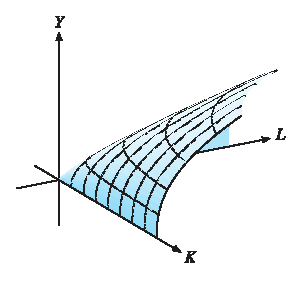
\includegraphics[width=\linewidth]{figure1}\label{fig:1}
			\caption{Gráfica de la función de producción Cobb-Douglas.}
		\end{minipage}
		\hfill
		\begin{minipage}[c]{0.4\linewidth}
			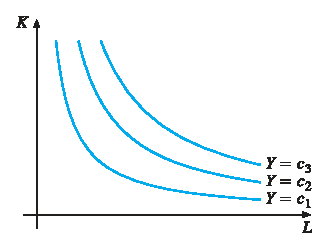
\includegraphics[width=\linewidth]{figure2}\label{fig:2}
			\caption{Isocuantas de la función de producción Cobb-Douglas.}
		\end{minipage}
	\end{figure}
\end{example}
% pag. 428
\begin{example}[Funciones $n$--lineales y $\log$--lineales]
	\leavevmode
	\begin{enumerate}
		\item\label{item:a} La demanda del azúcar en los Estados Unidos durante el período 1929--1936 fue estimado para ser descrito, aproximadamente, por la fórmula \[ x=108.83-6.0294p+0.164w-0.4217t \] donde $x$ es la demanda del azúcar, $p$ es su precio, $w$ es un índice de producción y $t$ es el año (donde $t=0$ corresponde a 1929).
		\item\label{item:b} La siguiente fórmula es una estimación para la demanda de cerveza en el Reino Unido: \[ x=1.058{x}^{0.136}_{1}{x}^{-0.727}_{2}{x}^{0.914}_{3}x^{0.816}_{4}. \]
		Aquí la cantidad demandada, $x$, es una función de cuatro variables: $x_{1}$, el ingreso per cápita, $x_{2}$, el precio de la cerveza, $x_{3}$, índice general de precios de productos básicos y $x_{4}$, la fuerza de la cerveza.
	\end{enumerate}
\end{example}
Las funciones más simples en el ejemplo anterior es la única en la parte~\eqref{item:a}. Las variables $p$, $w$ y $t$ ocurren solo cuando a la primera potencia, y ellas son multiplicadas por constantes, no por cada otra. Tales funciones son llamadas \emph{lineales}. En general
\begin{equation}
f\left(x_{1},x_{2},\ldots,x_{n}\right)=a_{1}x_{1}+a_{2}x_{2}+\cdots+a_{n}x_{n}+b
\end{equation}
donde $a_{1},a_{2},\ldots,a_{n}$ y $b$ son constantes, es una \emph{función lineal} en $n$ variables.

La función en la parte~\eqref{item:b} del ejemplo  es un caso especial de la función general de Cobb-Douglas
\begin{equation}\label{eq:cobbgeneralized}
F\left(x_{1},x_{2},\ldots,x_{3}\right)=A{x}^{a_{1}}_{1}{x}^{a_{2}}_{2}\cdots{x}^{a_{n}}_{n}
\end{equation}
donde $A>0$, $a_{1},\ldots,a_{n}$ son constantes, definidas para $x_{1}>0,x_{2}>0,\ldots x_{n}>0$. Note que al tomar el logaritmo natural a cada lado de~\eqref{eq:cobbgeneralized} resulta
\begin{equation}
\ln F=\ln A+a_{1}\ln x_{1}+a_{2}\ln x_{2}+\cdots+a_{n}\ln x_{n}.
\end{equation}
Esto muestra que la función de Cobb-Douglas es $\log$--lineal, ya que $\ln F$ es una función lineal para $\ln x_{1},\ln x_{2},\ldots,\ln x_{n}$.
% arara: lualatex: { draft: yes }
% arara: lualatex: { draft: yes }
% arara: pythontex
% !arara: biber
% arara: lualatex: { draft: yes }
% arara: lualatex: {
% arara: --> shell: yes,
% arara: --> synctex: yes,
% arara: --> interaction: batchmode
% arara: --> }
% arara: clean: {
% arara: --> extensions:
% arara: --> ['log','aux','out','pytxcode','synctex.gz','toc','bbl','bcf','blg', 'run.xml']
% arara: --> }
% arara: lualatex: { draft: yes }
% arara: lualatex: { draft: yes }
% arara: pythontex
% !arara: biber
% arara: lualatex: { draft: yes }
% arara: lualatex: {
% arara: --> shell: yes,
% arara: --> synctex: yes,
% arara: --> interaction: batchmode
% arara: --> }
% arara: clean: {
% arara: --> extensions:
% arara: --> ['log','aux','out','pytxcode','synctex.gz','toc','bbl','bcf','blg', 'run.xml']
% arara: --> }
\input{cobb-douglas.tex.preamble}
\begin{document}

\maketitle
\include{./contents/spanish/abstract}

\tableofcontents

\include{./contents/spanish/introduction}
\include{./contents/spanish/cobb-douglas}
\include{./contents/spanish/solow}
\include{./contents/spanish/inada}
\include{./contents/spanish/models}
\include{./contents/spanish/deduction}
\include{./contents/spanish/understandingsolow}
\include{./contents/spanish/crecimiento}
%\include{./contents/spanish/codification}
%\include{./contents/spanish/sympying}
%\include{./contents/spanish/references}

\appendix

%\include{./contents/spanish/performance}
%\include{./contents/spanish/linearregression}

\vfill
\begin{flushright}
Facultad de Ciencias, \today.
\end{flushright}

\include{./contents/english/abstract}

\tableofcontents

\vfill
\begin{flushright}
Science department, \today.
\end{flushright}

\end{document}
\begin{document}

\maketitle
\selectlanguage{spanish}

\begin{abstract}
La función de producción Cobb-Douglas es un enfoque neoclásico para estimar la función de producción de un país y proyectar de esta manera su crecimiento económico esperado. Para representar las relaciones entre la producción obtenida se utiliza las variaciones de los insumos como el capital ($K$) y el trabajo ($L$), a los que más tarde se añadió la tecnología, llamada también productividad total de los factores ($PTF$). Es una función de producción frecuentemente utilizada en Economía.
%https://assets.aeaweb.org/asset-server/files/9434.pdf

El origen de la función Cobb-Douglas se encuentra en la observación empírica de la distribución de la renta nacional total de Estados Unidos entre el capital y el trabajo. De acuerdo a lo que mostraban los datos, la distribución se mantenía relativamente constante a lo largo del tiempo. Concretamente el trabajo se llevaba un 70\% y el capital un 30\%. De esta forma, la función Cobb-Douglas representa una relación en donde las proporciones de trabajo y capital con respecto al producto total son constantes.%\pygment{python}{module}
\end{abstract}

\tableofcontents

\section{Introducción}

Este proyecto hace referencia a la función de producción de Cobb-Douglas, siendo este publicado en \cite{Douglas1976} 1928 por \citeauthor{Douglas1976}, quienes realizaron un estudio en el que se modeló el crecimiento de la economía estadounidense. Para este proyecto se desarrollará una aplicación con una base de datos como un caso particular, pero previo a su aplicación, se realizará una posible forma de cómo Charles Cobb y Paul Douglas llegaron a la formulación algebraica de la función. Al finalizar, se comparará la solución exacta de la ecuación con la obtenida por el método de mínimos cuadrados.

\subsection{Función de producción de Cobb-Douglas}

Para el análisis matemático de la función, es necesario describir los factores involucrados en el modelo.

\subsection{Función de producción}

Es la relación entre las cantidades máximas de productos que una empresa puede fabricar mediante el uso de diversas cantidades de insumos. Las múltiples funciones de producción están representadas por la combinación de factores de insumo (tecnología, capital, trabajo entre otros). Una función de producción se expresa como la ecuación~\eqref{eq:production} siguiente:
\begin{equation}\label{eq:production}
P=f(K,L,I)
\end{equation}
donde:
\begin{itemize}
	\item $P$ es la cantidad de producción.
	\item $K,L,I$ son los insumos.
\end{itemize}

\section{El proyecto}

En esta sección explicaré los detalles de mi proyecto y su visión. Espero que esta estructura se mejore considerablemente bajo la guía de mi mentor.

\subsection{Cobb-Douglas y la función de producción ACMS}

Partiendo de la función Cobb-Douglas
\begin{equation}%\label{eq:1}
Y = bL^{k}C^{1-k},
\end{equation}
donde:
\begin{itemize}
	\item $b$ representa el factor total de productividad,
	\item $Y$ la producción total,
	\item $L$ el trabajo,
	\item $C$ el capital.
\end{itemize}
Esta función fue generalizada siendo expresada de la manera siguiente:
\begin{equation}%\label{eq:2}
f = \gamma{x}_{1}^{\alpha_{1}}\cdots x_{n}^{\alpha_{n}},
\end{equation}
donde $\gamma$ es una constante positiva y $\alpha_{1},\ldots,\alpha_{n}$ son constantes no cero.

Se dice que una función de producción $f$ es $d$--homogénea o homogénea de degradación $d$, si:
\begin{equation}%\label{eq:3}
f\left(tx_{1},\ldots,tx_{n}\right) = t^{d}f\left(x_{1},\ldots,x_{n}\right),
\end{equation}
Se mantiene para cada $t\in\mathbb{R}$ en la función previamente definida.

Una función \emph{homogénea de degradación uno} es llamado como \emph{linealmente homogéneo}.

Si $d>1$, la función homogénea mostrará un crecimiento a escala, caso contrario cuando $d<1$ mostrará un decrecimiento a escala.

Arrow, Chenery, Minhas y Solow(ACMS) introdujeron una función de producción de dos factores:
\begin{equation}%\label{eq:4}
Q=F\cdot(aK^r + (1-a)L^r)^{1/r},
\end{equation}
donde:
\begin{itemize}
	\item $Q$ representa el resultado,
	\item $F$ el factor de producción,
	\item $a$ el parámetro compartido,
	\item $k,L$ los factores de producción primario,
	\item $r=\left(s-1\right)/s$ , $s=1/\left(1-r\right)$ como la substitución de elasticidad.
\end{itemize}

La función de producción generalizada de ACMS se define:
\begin{equation}\label{eq:5}
f\left(x\right) = \gamma\sum_{i=1}^{n} ({{a}_{i}^{p}x_{i}^{p}})^{d/p},x=\left(x_{1},\ldots,x_{n}\right)\in D\subset\mathbb{R}_{+}^{n},
\end{equation}
con $a_{1},\ldots,a_{n},\gamma,p\neq0$, donde $d$ es la degradación de homogeneidad.

Cabe resaltar que la \emph{función de producción homotética} tiene la siguiente expresión como una función de producción:
\begin{equation}\label{eq:6}
f(x) = F\left(h(x_1,\ldots,x_n\right),
\end{equation}
donde F es una función estrictamente creciente y $h\left(x_1,\ldots,x_n\right)$ es una función homogénea de cualquier degradación d. La \emph{función de producción homotética} de la forma:
\begin{equation}\label{eq:7}
f\left(x\right) = \gamma\sum_{i=1}^{n} ({{a}_{i}^{p}x_{i}^{p}})^{d/p},\quad(\text{resp.},\quad f(x)=F(x_{1}^{\alpha_1}\cdots x_{n}^{\alpha_n}),
\end{equation}
es llamada \emph{función de producción ACMS generalizada homotética}.

\subsection{Breve descripción}

Si $f$ es una función de dos variables, a menudo dejamos que una letra como $z$ denote el valor de $f$ en el punto $\left(x,y\right)$, así $z=f\left(x,y\right)$. Entonces llamaremos a $x$ e $y$ las \emph{variables independientes}, o los \emph{argumentos} de $f$, mientras que $z$ es llamada la \emph{variable independiente}, porque el valor $z$, en general, depende de los valores $x$ e $y$. El dominio de la función $f$ es entonces el conjunto de todos los posibles pares de variables independientes, mientras que su \emph{rango} es el conjunto de valores correspondientes de la variable dependientes. En economía, $x$ e $y$ son llamadas las variables \emph{exógenas}, mientras que $z$ es la variable \emph{endógena}.

Una función de dos variables que aparecen en muchos modelos económicos es
\begin{equation}\label{eq:cobb-douglas}
F\left(x,y\right)=Ax^{a}y^{b}
\end{equation}
donde $A$, $a$ y $b$ son constantes. Usualmente, uno asume que $F$ es definida solo para $x>0$ e $y>0$.

A función de la forma~\eqref{eq:cobb-douglas} es generalmente llamada la \emph{función de Coubb-Douglas}. Se usa con mayor frecuencia para describir ciertos procesos de producción. Entonces $x$ e $y$ son llamados \emph{factores de entrada}, mientras que $F\left(x,y\right)$ es el número de unidades producidas, o la \emph{salida}. En este caso $F$ es llamada la \emph{función de producción}.

%\subsubsection{Defining \pygment{python}{ImageSet} Union for Trigonometric Equation Solver}%\protect||

% TODO: Page 276.
\begin{example}[Elasticidad de sustitución constante]
	Considere la ``elasticidad de sustitución constante'', o la función \textsc{CES}
	\begin{equation}
	F\left(K,L\right)=A\left(aK^{-\rho}+\left(1-a\right)L^{-\rho}\right)^{-1/\rho}
	\end{equation}
	donde $A>0$, $K>0$, $L>0$, $a\in\left(0,1\right)$, y $\rho\neq 0$. Manteniendo $A,K,L$ y $a$ fijos, aplique la regla de L'H\^{o}pital a $z=\ln\left[F\left(K,L\right)/A\right]$  cuando $\rho\to0$ con el fin de mostrar que $F\left(K,L\right)$ converge a la función de Cobb-Douglas $AK^{a}L^{1-a}$.
\end{example}

\begin{proof}[Solución]
	Obtenemos \[ z=\ln{\left(aK^{-\rho}+\left(1-a\right)L^{-\rho}\right)}^{-1/\rho}=-\ln\left(aK^{-\rho}+\left(1-a\right)L^{-\rho}\right)/\rho\to\frac{0}{0}\text{ cuando }\rho\to0. \] Ya que $\left(\mathrm{d}/\mathrm{d}\rho\right)K^{-\rho}=-K^{-\rho}\ln K$ y $\left(\mathrm{d}/\mathrm{d}\rho\right)L^{-\rho}=-L^{-\rho}\ln L$, aplicando la regla de L'H\^{o}pital da
	\begin{align*}
	\lim_{\rho\to0}z
	&=\lim_{\rho\to0}\left[\frac{aK^{-\rho}\ln K + \left(1-a\right)L^{-\rho}\ln L}{aK^{-\rho}+\left(1-a\right)L^{-\rho}}\right]\\
	&=a\ln K+\left(1-a\right)\ln L\\
	&=\ln K^{a}L^{1-a}.
	\end{align*}
	Por lo tanto, $e^{z}\to K^{a}L^{1-a}$. De la definición de $z$, se sigue que $F\left(K,L\right)\to AK^{a}L^{1-a}$ cuando $\rho\to0$.
\end{proof}

%pag. 408-409
\begin{example}[Función de Cobb-Douglas]
	Una función de dos variables que aparece en muchos modelos económicos es
	\begin{equation}\label{eq:cobb}
	F\left(x,y\right)=Ax^{a}y^{b}
	\end{equation}
	donde $A$, $a$ y $b$b son constantes. Usualmente, uno asume que $F$ está definida sola pora $x>0$ e $y>0$.

	Una función $F$ de la forma~\eqref{eq:cobb} es generalmente llamada la \emph{función de Cobb-Douglas}\footnote{La función en~\eqref{eq:cobb} es llamada en honor a los investigadores americanos C.W.Cobb y P.H.Douglas, quien aplicaron esto, con  $a+b=1$, en un articulo científico que aparecio en 1927 en la estimacion de una función de producción. Sin embargo, deberia correctamente ser llamada la ``función de Wicksell'', porque el economista sueco K.Wicksell(1851-1926) introdujo tales funciones de producción antes de 1900.}. Con frecuencia es usada para describir ciertos procesos productivos. Así, $x$ e $y$ son llamados los \emph{factores de entrada}, mientras que $F\left(x,y\right)$ es el número de unidades producidas, o la \emph{salida}. En este caso, $F$ es llamada una \emph{función de producción}.
\end{example}

\begin{example}
	Suponga que $F\left(K,L\right)$ modela la producción de una empresa cuando sus entradas son capital y labor, respectivamente $K$ y $L$. Una curva de nivel por esta función de producción es una curva en el plano $KL$ dado por $F\left(K,L\right)=Y_{o}$, donde $Y_{0}$ es una constante. Esta curva es llamada una \emph{isocuanta}, que significa ``igual cantidad''. Para una función de Cobb-Douglas, $F\left(K,L\right)=AK^{a}L^{b}$, con $a+b<1$ y $A>0$, las figuras~\ref{fig:1} y~\ref{fig:2}, respectivamente, muestra una parte de la gráfica cerca del origen, y tres de las isocuantas.
	
	\begin{figure}[ht!]
		\begin{minipage}[c]{0.4\linewidth}
			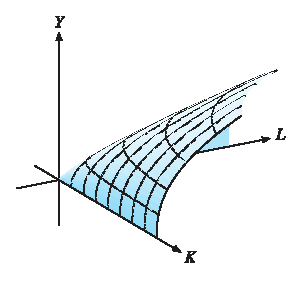
\includegraphics[width=\linewidth]{figure1}\label{fig:1}
			\caption{Gráfica de la función de producción Cobb-Douglas.}
		\end{minipage}
		\hfill
		\begin{minipage}[c]{0.4\linewidth}
			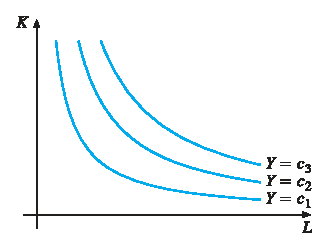
\includegraphics[width=\linewidth]{figure2}\label{fig:2}
			\caption{Isocuantas de la función de producción Cobb-Douglas.}
		\end{minipage}
	\end{figure}
\end{example}
% pag. 428
\begin{example}[Funciones $n$--lineales y $\log$--lineales]
	\leavevmode
	\begin{enumerate}
		\item\label{item:a} La demanda del azúcar en los Estados Unidos durante el período 1929--1936 fue estimado para ser descrito, aproximadamente, por la fórmula \[ x=108.83-6.0294p+0.164w-0.4217t \] donde $x$ es la demanda del azúcar, $p$ es su precio, $w$ es un índice de producción y $t$ es el año (donde $t=0$ corresponde a 1929).
		\item\label{item:b} La siguiente fórmula es una estimación para la demanda de cerveza en el Reino Unido: \[ x=1.058{x}^{0.136}_{1}{x}^{-0.727}_{2}{x}^{0.914}_{3}x^{0.816}_{4}. \]
		Aquí la cantidad demandada, $x$, es una función de cuatro variables: $x_{1}$, el ingreso per cápita, $x_{2}$, el precio de la cerveza, $x_{3}$, índice general de precios de productos básicos y $x_{4}$, la fuerza de la cerveza.
	\end{enumerate}
\end{example}
Las funciones más simples en el ejemplo anterior es la única en la parte~\eqref{item:a}. Las variables $p$, $w$ y $t$ ocurren solo cuando a la primera potencia, y ellas son multiplicadas por constantes, no por cada otra. Tales funciones son llamadas \emph{lineales}. En general
\begin{equation}
f\left(x_{1},x_{2},\ldots,x_{n}\right)=a_{1}x_{1}+a_{2}x_{2}+\cdots+a_{n}x_{n}+b
\end{equation}
donde $a_{1},a_{2},\ldots,a_{n}$ y $b$ son constantes, es una \emph{función lineal} en $n$ variables.

La función en la parte~\eqref{item:b} del ejemplo  es un caso especial de la función general de Cobb-Douglas
\begin{equation}\label{eq:cobbgeneralized}
F\left(x_{1},x_{2},\ldots,x_{3}\right)=A{x}^{a_{1}}_{1}{x}^{a_{2}}_{2}\cdots{x}^{a_{n}}_{n}
\end{equation}
donde $A>0$, $a_{1},\ldots,a_{n}$ son constantes, definidas para $x_{1}>0,x_{2}>0,\ldots x_{n}>0$. Note que al tomar el logaritmo natural a cada lado de~\eqref{eq:cobbgeneralized} resulta
\begin{equation}
\ln F=\ln A+a_{1}\ln x_{1}+a_{2}\ln x_{2}+\cdots+a_{n}\ln x_{n}.
\end{equation}
Esto muestra que la función de Cobb-Douglas es $\log$--lineal, ya que $\ln F$ es una función lineal para $\ln x_{1},\ln x_{2},\ldots,\ln x_{n}$.
% arara: lualatex: { draft: yes }
% arara: lualatex: { draft: yes }
% arara: pythontex
% !arara: biber
% arara: lualatex: { draft: yes }
% arara: lualatex: {
% arara: --> shell: yes,
% arara: --> synctex: yes,
% arara: --> interaction: batchmode
% arara: --> }
% arara: clean: {
% arara: --> extensions:
% arara: --> ['log','aux','out','pytxcode','synctex.gz','toc','bbl','bcf','blg', 'run.xml']
% arara: --> }
\input{cobb-douglas.tex.preamble}
\begin{document}

\maketitle
\include{./contents/spanish/abstract}

\tableofcontents

\include{./contents/spanish/introduction}
\include{./contents/spanish/cobb-douglas}
\include{./contents/spanish/solow}
\include{./contents/spanish/inada}
\include{./contents/spanish/models}
\include{./contents/spanish/deduction}
\include{./contents/spanish/understandingsolow}
\include{./contents/spanish/crecimiento}
%\include{./contents/spanish/codification}
%\include{./contents/spanish/sympying}
%\include{./contents/spanish/references}

\appendix

%\include{./contents/spanish/performance}
%\include{./contents/spanish/linearregression}

\vfill
\begin{flushright}
Facultad de Ciencias, \today.
\end{flushright}

\include{./contents/english/abstract}

\tableofcontents

\vfill
\begin{flushright}
Science department, \today.
\end{flushright}

\end{document}
\section{Introducción}
Cualquier teoría depende de supuestos que no son del todo ciertos. Eso es lo que lo hace teoría. El arte de teorizar con éxito es hacer los supuestos simplificadores inevitables de tal manera que los resultados finales no sean muy sensibles. Una suposición ``crucial'' es una de las cuales las conclusiones dependen sensiblemente, y es importante
que los supuestos cruciales sean razonablemente realistas. Cuando los resultados de una teoría parecen fluir específicamente de una suposición crucial especial, entonces, si la suposición es dudosa, los resultados son sospechosos.

Deseo argumentar que algo así es cierto en el modelo de crecimiento económico Harrod--Domar. La característica y poderosa conclusión de la línea de pensamiento Harrod--Domar es que incluso para el largo plazo, el sistema económico está en el mejor de los casos equilibrado sobre el filo del cuchillo del equilibrio del crecimiento. ¿Eran las magnitudes de los parámetros clave --la relación de ahorro, la relación capital-producto, la tasa de aumento de la mano de obra--si se deslizara un poco desde el punto muerto, la consecuencia sería un desempleo creciente o una inflación prolongada. En términos de Harrod, la cuestión crítica del equilibrio se reduce a una comparación entre la tasa natural de crecimiento que depende, en la ausencia del cambio tecnológico, en el aumento de la fuerza laboral, y la tasa de crecimiento garantizada que depende de los hábitos de ahorro e inversión de los hogares y las empresas.

Pero esta oposición fundamental de tasas garantizadas y naturales al final resulta que parte del supuesto crucial de que la producción tiene lugar en condiciones de \emph{proporciones fijas}. No hay posibilidad de sustituir mano de obra por capital en producción. Si esta suposición se abandona, la noción del filo de cuchillo de equilibrio inestable parece ir con eso. De hecho, no es sorprendente que una rigidez tan grave en una parte del sistema implique falta de flexibilidad en otro.

Una característica notable del modelo Harrod--Domar es que estudia constantemente los problemas a largo plazo con las herramientas de corto plazo habitual. Normalmente se piensa en el largo plazo como el dominio del análisis neoclásico, la tierra del margen. En cambio Harrod y Domar hablan del largo plazo en términos del multiplicador, el acelerador, ``el'' coeficiente de capital. La mayor parte de este documento está dedicado a un modelo de crecimiento a largo plazo que acepta todos los supuestos de Harrod--Domar excepto el de proporciones fijas. En cambio supongo que la única mercancía compuesta es producida por trabajo y capital bajo las condiciones neoclásicas estándar. La adaptación del sistema a una tasa de incremento de la fuerza laboral dada de manera exógena se calcula en algún detalle, para ver si aparece la inestabilidad de Harrod. Las reacciones de interés precio-salario juegan un papel importante en este proceso de ajuste neoclásico, por lo que también se analizan. Luego, algunos de los otros rígidos supuestos se relajan ligeramente para ver qué cambios cualitativos resultan: se permite un cambio tecnológico neutral y un interés elástico horario de ahorro. Finalmente, las consecuencias de ciertas relaciones y rigideces más ``keynesianas'' son brevemente consideran.

\section{Un modelo de crecimiento a largo plazo}
Solo hay una mercancía, la producción como un todo, cuya tasa de producción se designa $Y\left(t\right)$. Así podemos hablar inequívocamente del ingreso real de la comunidad. Parte de cada salida instantánea es consumida y el resto se ahorra e invierte. La fracción de la salida ahorrada es una constante $s$, de modo que la tasa de ahorro es $sY\left(t\right)$. El stock de capital de la comunidad $K\left(t\right)$ toma la forma de una acumulación de la mercancía compuesta. La inversión neta es solo la tasa de
aumento de este capital social $\mathrm{d}K/\mathrm{d}t$ o $\dot{K}$, por lo que tenemos la identidad básica en cada instante de tiempo:
\begin{equation}\label{eq:first}
\dot{K}=sY
\end{equation}
La salida es producida con la ayuda de dos factores de producción, capital y trabajo, cuya tasa de ingreso es $L\left(t\right)$. Las posibilidades tecnológicas son representadas por una función de producción.
\begin{equation}\label{eq:second}
Y=F\left(K,L\right)
\end{equation}
La salida es entendida como la salida neta después de hacer buena la depreciación del capital. Sobre la producción, todo lo que diremos en este momento es que muestra rendimientos constantes a escala. Por lo tanto, la función de producción es homogénea de primer grado. Esto equivale a asumir que no existe un recurso escaso no aumentable como la tierra. Retornos de escala constante parece la suposición natural para hacer en una teoría de crecimiento. El caso de tierras escasas conduciría a rendimientos decrecientes a
escala en capital y trabajo y el modelo se volvería más Ricardiano.

Insertando~\eqref{eq:second} en~\eqref{eq:first} obtenemos
\begin{equation}\label{eq:third}
\dot{K}=sF\left(K,L\right).
\end{equation}
Este es una ecuación con dos incógnitas. Una primera manera de acercarse al sistema sería agregar una ecuación de demanda de trabajo: la productividad física del trabajo marginal es igual a la tasa salarial real; y una ecuación de oferta de trabajo. Este último podría tomar la forma general de hacer trabajo proporcionar una función del salario real, o más clásico de poner el salario real igual a un nivel de subsistencia convencional. En cualquier caso serían tres ecuaciones en las tres incógnitas $K$, $L$, salario real.

En cambio, procedemos más en el espíritu del modelo Harrod. Como un resultado exógeno del crecimiento de la población, la fuerza laboral aumenta a una tasa relativa constante $n$. En ausencia de cambio tecnológico, $n$ es la tasa natural de crecimiento de Harrod. Así:
\begin{equation}\label{eq:fourth}
L\left(t\right)=L_{0}e^{nt}
\end{equation}
En~\eqref{eq:third} $L$ representa el empleo total; en~\eqref{eq:fourth} $L$ representa la oferta de trabajo disponible. Al identificar los dos estamos asumiendo que el empleo se mantiene perpetuamente. Cuando insertamos~\eqref{eq:fourth} en~\eqref{eq:third} obtenemos
\begin{equation}\label{eq:fifth}
\dot{K}=sF\left(K,L_{0}e^{nt}\right)
\end{equation}
tenemos la ecuación básica que determina el camino temporal de la acumulación del capital que debe ser serguida si todas los trabajos disponibles están empleados.

Alternativamente,~\eqref{eq:fourth} puede ser visto como una curva de oferta de mano de obra. Eso dice que la fuerza laboral que crece exponencialmente se ofrece para un empleo completamente inelástico. La curva de oferta de trabajo es una línea vertical que se mueve hacia la derecha en el tiempo a medida que la fuerza laboral crece de acuerdo
para~\eqref{eq:fourth}. Luego, la tasa salarial real se ajusta para que toda la mano de obra disponible sea empleado, y la ecuación de productividad marginal determine la tasa salarial que realmente gobernará.

En resumen,~\eqref{eq:fifth} es una ecuación diferencial con la única variable $K\left(t\right)$. Su solución da el único perfil de tiempo del capital social de la comunidad que empleará plenamente la mano de obra disponible. Una vez que nosotros conozca el camino temporal del stock de capital y el de la fuerza laboral, podemos calcular desde la función de producción la ruta de tiempo correspondiente de salida real. La ecuación de productividad marginal determina la trayectoria temporal del salario real. También hay una suposición involucrada de pleno empleo del stock de capital disponible. En cualquier punto de tiempo en que el stock de capital preexistente (el resultado de una acumulación previa) se suministra de manera inelástica. Por lo tanto, existe una ecuación de productividad marginal similar para el capital que determina el alquiler real por unidad de tiempo para los servicios de capital social. El proceso puede ser visto de esta manera: en cualquier momento la oferta laboral disponible está dado por~\eqref{eq:fourth} y el stock de capital disponible también es un dato. Ya que el rendimiento real de los factores se ajustará para lograr el pleno empleo de trabajo y capital podemos usar la función de producción~\eqref{eq:second} para encontrar la tasa actual de salida. Entonces la propensión a ahorrar nos dice cuánto de la producción neta se ahorrará e invertirá. Por eso conocemos la acumulación del capital neta durante el período actual. Agregado al stock ya acumulado, esto da el capital disponible para el próximo período, y todo el proceso puede repetirse.
\section{Posibles patrones de crecimiento}
Para ver si siempre existe una ruta de acumulación de capital consistente con cualquier tasa de crecimiento de la fuerza laboral, debemos estudiar la ecuación diferencial~\eqref{eq:fifth} por la naturaleza cualitativa de sus soluciones. Naturalmente sin especificar la forma exacta de la función de producción no podemos esperar encontrar la solución exacta. Pero ciertas propiedades amplias son sorprendentemente fáciles de aislar, incluso gráficamente.

Para ello, introducimos una nueva variable $r=\frac{K}{L}$, la relación de capital al trabajo Por lo tanto, tenemos $K=rL=rL_{0}e^{nt}$. Diferenciando con respecto al tiempo que tenemos
\begin{equation}
\dot{K}=L_{0}e^{nt}r^{\prime}+nrL_{0}e^{nt}.
\end{equation}
Reemplazando esto en~\eqref{eq:fifth}: \[ \left(\dot{r}+nr\right)L_{0}e^{nt}=sF\left(K,L_{0}e^{nt}\right). \] Pero debido al retorno de escala constante podemos dividir ambas variales en $F$ por $L=L_{0}e^{nt}$, no obstante, multiplicamos $F$ por el mismo factor. Así \[ \left(\dot{r}+nr\right)L_{0}e^{nt}=sLe^{nt}F\left(\frac{K}{L_{0}e^{nt}},1\right) \] y dividiendo el factor común llegamos finalmente a
\begin{equation}\label{eq:sixth}
\dot{r}=sF\left(r,1\right)-nr.
\end{equation}
Aquí tenemos una ecuación diferencial que involucra solamente la relación capital-trabajo.

Esta ecuación fundamental se puede alcanzar menos formalmente. Como $r=\frac{K}{L}$, la tasa de cambio relativa de $r$ es la diferencia entre las tasas relativas de cambio de $K$ y $L$. Eso es: \[ \frac{\dot{r}}{r}=\frac{\dot{K}}{K}-\frac{\dot{L}}{L}. \] Ahora primero que nada $\frac{\dot{L}}{L}=n$. En segundo lugar, $\dot{K}=sF\left(K,L\right)$. Haciendo estas substituciones: \[ \dot{r}=r\frac{sF\left(K,L\right)}{K}-nr. \] Ahora divida $L$ de $F$ como antes, note que que $\frac{L}{K}=\frac{1}{r}$ y obtenemos~\eqref{eq:sixth} nuevamente.

La función $F\left(r,1\right)$ que aparece en~\eqref{eq:sixth} es fácil de interpretar. Esta es la curva del producto total cuando varían las cantidades $r$ de capital con una unidad de trabajo. Alternativamente, da salida por trabajador como una función de capital por trabajador. Así~\eqref{eq:sixth} establece que la tasa del cambio de la relación capital-trabajo es la diferencia de dos términos, uno representando el incremento de capital y uno el incremento de trabajo.

Cuando $\dot{r}=0$, la relación capital-trabajo es una constante, y el capital existente debe expandirse al mismo ritmo que la fuerza laboral, es decir, $n$.

(La tasa de crecimiento garantizada, garantizada por la tasa real apropiada de retorno al capital, es igual a la tasa natural.) En la Figura I, el rayo que pasa por el origen con pendiente $n$ representa la función $nr$. La otra curva es la función $sF\left(r,1\right)$. Aquí se dibuja para pasar por el origen y convexo hacia arriba: sin salida a menos que ambas entradas sean positivas, y la disminución de la productividad marginal del capital, como sería el caso, por ejemplo, con la función Cobb-Douglas. En el punto de intersección $nr=sF\left(r,1\right)$ y $\dot{r}=0$. Si la relación capital-trabajo $r^{\ast}$ debe establecerse, se mantendrá, y el capital y
el trabajo crecerá de allí en adelante en proporción. Por la constante retornos a escala

\newpage
Formalmente, una función de producción se define para tener:
\begin{itemize}
	\item Constante retorno a escala si (para cualquier constante $a$ es mayor que $0$) $F\left(aK,aL\right)=aF\left(K,L\right)$ (Función $F$ es homogénea de grado $1$).
	\item Retornos a escala crecientes si (para cualquier constante mayor que $1$) $F\left(aK,aL\right)>aF\left(K,L\right)$.
	\item Retornos a escala decrecientes si (para cualquier constante $a$ mayor que $1$) $F\left(aK,aL\right)<aF\left(K,L\right)$.
\end{itemize}
donde $K$ y $L$ son factores de producción--capital y trabajo, respectivamente.

En una configuración más general, para procesos de producción de múltiples entradas y múltiples salidas, se puede suponer que la tecnología se puede representar a través de algún conjunto de tecnología, llámelo $T$ que debe satisfacer algunas condiciones de regularidad de la teoría de la producción. En este caso, la propiedad de retorno de escala constante es equivalente a decir que el conjunto tecnológico es un cono, es decir, satisface la propiedad $aT=T$, $\forall a>0$. A su vez, si hay una función de producción que describirá el conjunto de tecnología $T$, deberá ser homogéneo de grado $1$.


\begin{definition}[Rendimiento de escala]
	La forma funcional de Cobb-Douglas tiene una constante retorno de escala cuando la suma de sus exponentes es $1$. En este caso, la función es
	\begin{equation}
	F\left(K,L\right)=AK^{b}L^{1-b}
	\end{equation}
	donde $A>0$ y $0<b<1$. Así \[ F\left(aK,aL\right)=A{\left(ak\right)}^{b}{\left(aL\right)}^{1-b}=Aa^{b}a^{1-b}K^{b}L^{1-b}=aAK^{b}L^{1-b}=aF\left(K,L\right). \] Aquí como entrada usamos todas las escalas por un factor multiplicador $a$, la salida también escala por $a$ y así existen constantes de retorno de escala.
	
	Pero, si la función de producción de Cobb-Douglas tiene su forma general
	\begin{equation}
	F\left(K,L\right)=AK^{b}L^{c}
	\end{equation}
	donde $0<b<1$ y $0<c<1$, entonces existen retornos crecientes si $b+c>1$, pero retornos decrecientes si $b+c<1$, dado que \[ F\left(aK,aL\right)=A{\left(aK\right)}^{b}{\left(aL\right)}^{c}=Aa^{b}a^{c}K^{b}L^{c}=a^{b+c}AK^{b}L^{c}=a^{b+c}F\left(K,L\right), \] que para $a>1$ es mayor que o menor que $aF\left(K,L\right)$ cuando $b+c$ es mayor o menor que uno.
\end{definition}

Hay dos clases especiales de funciones de producción que a menudo se analizan. La función de producción $Q=f\left(X_{1},X_{2},\ldots,X_{n}\right)$ se dice que es homogéneo de grado $m$, si se le da alguna constante positiva $k$, $f\left(kX_{1},kX_{2},\ldots,kX_{n}\right)=k^{m}f\left(X_{1},X_{2},\ldots, X_{n}\right)$. Si $m>1$, la función exhibe rendimientos crecientes a escala, y exhibe rendimientos decrecientes a escala si $m<1$. Si es homogéneo de grado $1$, exhibe rendimientos constantes a escala. La presencia de rendimientos crecientes significa que un aumento del uno por ciento en los niveles de uso de todas las entradas daría como resultado un aumento de más del uno por ciento en la producción; la presencia de rendimientos decrecientes significa que daría como resultado un aumento de producción de menos del uno por ciento. Los retornos constantes a escala son el caso intermedio. En la función de producción Cobb–Douglas mencionada anteriormente, los rendimientos a escala aumentan si $a_{1}+a_{2}+\cdots+a_{n}> 1$, disminuyendo si $a_{1}+a_{2}+\cdots+a_{n}<1$, y constante si $a_{1}+a_{2}+\cdots+a_{n}=1$.

Si una función de producción es homogénea y de grado uno, este a veces llamada ``linealmente homogénea''. Una función de producción linealmente homogénea con entradas capital y labor tienen las propiedades de que los productos físicos marginales y promedio tanto del capital como del trabajo pueden expresarse solamente como funciones de la relación capital-trabajo. Además, en este caso, si cada entrada se paga a una tasa igual a su producto marginal, los ingresos de la empresa se agotarán exactamente y no habrá ganancias económicas excesivas.

Las funciones homotéticas son funciones cuya tasa de sustitución técnica marginal (la pendiente de la isocuanta, una curva dibujada a través del conjunto de puntos en dicho espacio de trabajo-capital en el que se produce la misma cantidad de producción para combinaciones variables de las entradas) es homogénea de grado cero Debido a esto, a lo largo de los rayos que provienen del origen, las pendientes de las isocuantas serán las mismas. Las funciones homotéticas tienen la forma $F\left(h\left(X_{1},X_{2}\right)\right)$ donde $F(y)$ es una función monótona creciente (la derivada de $F\left(y\right)$ es positiva $\mathrm{d}F/\mathrm{d}y>0$, y la función $h\left(X_{1},X_{2}\right)$ es una función homogénea de cualquier grado.

La elasticidad de sustitución constante (CES), en economía, es una propiedad de algunas funciones de producción y funciones de utilidad.

Específicamente, este en un tipo particular de función agregado que combina dos o más tipos de productos de consumos, o dos o más tipos de entradas de producción dentro de un cantidad agregado. Esta función de agregación exhibe una elasticidad de sustitución constante.
\begin{definition}[Elasticidad de sustitución constante]
La función de producción CES es una función de producción neoclásica que muestra una elasticidad de sustitución constante. En otras palabras, la producción tecnológica tiene un porcentaje de cambio constante en factores (por ejemplo, trabajo y capital) proporcional debido al cambio porcentual en la tasa marginal de la sustitución técnica. Los dos factores (capital y trabajo) de la función de producción fue introducido por Solow y más tarde popularizado por Arrow, Chenery, Minhas y Solow es
\begin{equation}
Q=F\cdot{\left(a\cdot K^{\rho}+\left(1-a\right)\cdot L^{\rho}\right)}^{\frac{v}{\rho}}
\end{equation}
donde
\begin{itemize}
	\item $Q$ es la cantidad de salida,
	\item $F$ es el factor de productividad,
	\item $a$ es el parámetro forma,
	\item $K,L$ son las cantidades de los factores de producción primario (capital y trabajo)
	\item $\rho=\frac{\sigma-1}{\sigma}$ es el parámetro de sustitución,
	\item $\sigma=\frac{1}{1-\rho}$ es elasticidad de sustituación,
	\item $v$ es el grado de homogeneidad de la función de producción. Donde $v=1$ es el retorno de escala constante, $v<1$ es el retorno de escala decreciente y $v>1$ es el retorno de escala creciente.
\end{itemize}
Como su nombre lo sugiere, la función de producción CES exhibe una elasticidad de sustitución constante entre el capital y el trabajo. Leontief, linear y las funciones de Cobb-Douglas son casos especiales de la función de producción CES. Esto es,
\begin{itemize}
	\item Si $\rho$ se aproxima a $1$, tenemos una lineal o función de sustituto perfecto.
	\item Si $\rho$ se aproxima a cero en el límite, obtenemos la función de producción de Cobb-Douglas.
	\item Si $\rho$ se aproxima al menos infinito, obtenemos la Leontief o función de producción perfecta complementaria.
\end{itemize}
La forma general de la función de producción CES, con $n$ entradas, es
\begin{equation}
Q=F\cdot{\left[\sum_{i=1}^{n}a_{i}X^{r}_{i}\right]}^{\frac{1}{r}}
\end{equation}
donde
\begin{itemize}
	\item $Q$ es cantidad de salida
	\item $F$ es el factor de productividad
	\item $a_{i}$ es el parámetro forma de la entrada $i$, $\sum_{i=1}^{n}a_{i}=1$
	\item $X_{i}$ son las cantidades de los factores de producción, $i=1,2,\ldots,n$.
	\item $s=\frac{1}{1-r}$ es la elasticidad de sustitución.
\end{itemize}
\end{definition}
Extendiendo la forma función CES (Solow) para acomodar los múltiples factores de producción crea algunos problemas. Sin embargo, no existe una forma completamente general para hacer esto. Uzawa mostró que solo $n$ factores posibles de la función de producción $n>2$ con elasticidades de sustitución parciales constantes requiere o todas las elasticidades entre pares de factores son idénticas, o si alguna difiere, todo ellos deben ser igual a cada otra y todas las elasticidades restantes deben ser unitarias. Esto es verdad para cualquier función de producción. Esto significa el uso de la forma funcional CES para más dos factores significará general que no existe una elasticidad de sustitución entre todos los factores.

Las funciones CES anidades son comúnmente encontradas en los modelos de equilibrio parcial y equilibrio general. Diferentes anidamientos (niveles) permiten la introducción de las elasticidades de sustitución apropiadas.

\begin{definition}[Función de utilidad CES]
La misma forma funcional CES alcanza como una función de utilidad en la teoría del consumidor. Por ejemplo, si existen $n$ tipos de productos de consumos $x_{i}$, entonces el consumo agregado $X$ podría definirse usando el agregado CES:
\begin{equation}
X={\left[\sum_{i=1}^{n}a^{\frac{1}{s}}_{i}x^{\frac{s}{s-1}}_{i}\right]}^{\frac{s}{s-1}}
\end{equation}
Aquí nuevamente, los coeficientes $a_{i}$ son los parámetros forma y $s$ es la elasticidad de sustitución. Por lo tanto, los productos de consumo $x_{i}$ son perfectos sustitutos cuando $s$ se aproxima al infinito y complemento perfecto cuando $s$ se aproxima a cero. El agregado CES es también algunas veces llamado el \emph{agregador Armington}, el cual fue discutido por Armington (1969).

Las funciones de utilidad CES son un caso especial de las preferencias homotéticas.

El siguiente es un ejemplo de la función de utilidad CES para dos productos, $x$ e $y$ con igualdad compartidad:
\begin{equation}
u\left(x,y\right)={\left(x^{r}+y^{r}\right)}^{1/r}.
\end{equation}
La función expendidora en el caso es:
\begin{equation}
e\left(p_{x},p_{y},u\right)={\left(p^{r/\left(r-1\right)}_{x}+p^{r/\left(r-1\right)}_{y}\right)}^{\left(r-1\right)/r}\cdot u.
\end{equation}
La función de utilidad indirecta tiene su inversa:
\begin{equation}
v\left(p_{x},p_{y},I\right)={\left(p^{r/\left(r-1\right)}_{x}+p^{r/\left(r-1\right)}_{y}\right)}^{\left(1-r\right)/r}\cdot I.
\end{equation}
La funciones de demanda son:
\begin{align*}
x\left(p_{x},p_{y},I\right)
&=\frac{p^{1/\left(r-1\right)}_{x}}{p^{r/\left(r-1\right)}_{x}+p^{r/\left(r-1\right)}_{y}}\cdot I\\
y\left(p_{x},p_{y},I\right)
&=\frac{p^{1/\left(r-1\right)}_{y}}{p^{r/\left(r-1\right)}_{x}+p^{r/\left(r-1\right)}_{y}}\cdot I\\
\end{align*}
La función de utilidad CES es uno de los casos considerados por Dixit y Stiglitz (1977) en su estudio de la diversidad del producto optimal en el contexto de la competición monopolística.

Note que la diferencial entre la utilidad CES y la utilidad isoelástica: La función de utilidad CES es una función de utilidad ordinal que representa las preferencias sobre consumo seguro %TODO: Wikipedia https://en.wikipedia.org/wiki/Constant_elasticity_of_substitution
mientras que la función de utilidad isoelástica es una función de utilidad cardinal que representa en loterías. Una función de utilidad CES indirecta (dual) ha sido usado para derivar la marca de consistencia-utildidad de sistemas donde la demanda categórica son determinadas endógenamente por un multicategorizador, la función de utilidad CES indirecto. Esto también se ha muestro que las preferencias son autoduales y ambos son primales y duales % TODO:
podrían exhibir cualquier grado de convexidad.
\end{definition}
La existencia y la estabilidad relativa de un único crecimiento balanceado para modelos multisectoriales fueron establecidos por Solow y Samuelson bajo el supuesto de \emph{retorno de escala constante}. Ellos estudiaron dos tipos de sistemas de ecuaciones: el sistema de ecuación en \emph{diferencias} y el sistema de ecuación diferencial. Later Muth y Suit estudiaron el sistema formado bajo el supuesto de retorno de escala decreciente. El primer objetivo de este artículo es estudiar algún sistema de ecuación diferencial bajo los supuestos más débiles que los impuestos por Solow y Samuelson, pero que retenga el supuesto de \emph{retorno constante} de escala. El segundo objetivo es investigar cierto sistema de ecuación diferencial bajo el supuesto de \emph{retorno de escala decreciente}.

\subsection{Retorno de escala constante -- Caso general}
Nuestro sistema es expresado por las siguientes ecuaciones:
\begin{equation}
\dot{X}_{i}=H^{i}\left(X_{1},\ldots,X_{n}\right),\quad\left(i=1,\ldots,n\right).
\end{equation}
El sistema de arriba es modelo de crecimiento balanceado de Solow--Samuelson. Los $H^i$'s son definidos para cualquier $\left(X_{1},\ldots,X_{n}\right)\geq0$ y son asumidos que son continuas con respecto a cualquier variable y positivamente homogénea de grado uno. A lo largo del artículo, los $X_{i}$'s son restringidos a valores no negativos. Además, las funciones son solo definidas para valores no negativos. Esto es asumido que
\begin{equation}
H^{i}\text{ es no decreciente en todas las variables, excepto en }X^{i},
\end{equation}
y que
\begin{equation}
\left\{H^{1},\ldots,H^{n}\right\}\text{ es indescomponible}.
\end{equation}
Aquí la indescomposibilidad es definido como en Morishima. Esto es, para cualquier conjunto de índices $R=\left\{i_{i},\ldots,i_{r}\right\}$, las relaciones $X_{i}=X^{\prime}_{i}$ para $i\in R$ y $X_{l}<X^{\prime}_{l}$ para $l\notin R$ implica que existe por lo menos un $i\in R$ tal que $H^{i}\left(X_{1},\ldots,X_{n}\right)<H^{i}\left(X^{\prime}_{i},\ldots,X^{\prime}_{n}\right)$. Requerimos que $H^{i}$ sea no decreciente en $X_{j}$, para $j\neq i$, sin la restricción sobre la dependencia de $H^{i}$ sobre $X_{i}$. En contraste del supuesto de Solow y Samuelson que $H^{i}$ es creciente en todos los $X_{j}$.

Ddas sus supuestos y la homogeneidad de $H^{i}$ $\left(i=1,\ldots,n\right)$, este sigue que $H^{i}\geq0$ $(i=1,\ldots,n)$ para $X_{j}\geq0$ $(j=1,\ldots,n)$, y que, $H^{i}=0$  para todo $i$, si y solo si $X_{j}=0$ para todo $j$. En nuestro caso, sin embargo, $H^{i}$ no es necesariamente creciente en $X$. Por ello, no podemos obtener las propiedades mencionadas arriba. Así, asumimos ellos. Esto es, podemos asumir que
\begin{equation}
H^{i}\geq0\quad(i=1,\ldots,n)\text{ para }X_{j}\geq0\quad\left(j=1,\ldots,n\right).
\end{equation}
Entonces, de la indescomposabilidad y la homogeneidad de $H^{i}$, $H^{i}=0$ para todo $i$, si y solo si $X_{j}=0$ para todo $j$. Nuestro ánimo es probar el siguiente teorema.

\begin{theorem}
	Para el sistema de ecuaciones diferenciales, %TODO
	existe un único determinado positivo autovalor, estrictamente un único positivo autovector normalizado y así un único camino de crecimiento balanceado. Más aún, cualquier solución del camino del sistema relativamente se aproxima al camino de crecimiento balanceado.
\end{theorem}
\begin{proof}
Podemos mostrar por un procedimiento similar al de Solow y Samuelson sobre la existencia de un autovalor positivo $\lambda$ y un autovector no negativo, no nulo $V=\left(V_{1},V_{2},\ldots,V_{n}\right)$ tal que
\begin{align*}
\lambda V_{1}&=H^{1}\left(V_{1},\ldots,V_{n}\right),\\
&=\vdots\\
\lambda V_{n}&=H^{n}\left(V_{1},\ldots,V_{n}\right).
\end{align*}
Mostraremos que \emph{todas las componentes del autovector} $V$ \emph{son positivas}. Suponga que algunas componentes de $V$ son ceros. Sin pérdida de generalidad, podríamos suponer que \[ V_{i}=0\quad\text{para }i\leq r(<n), \] y \[ V_{i}>0\quad\text{ para }n\geq i>r. \] Entonces,
\begin{align*}
0&=H^{1}\left(0,\ldots0,V_{r+1},\ldots,V_{n}\right),\\
&=\vdots
0&=H^{r}\left(0,\ldots0,V_{r+1},\ldots,V_{n}\right),\\
0<\lambda V_{r+1}&=H^{r+1}\left(0,\ldots0,V_{r+1},\ldots,V_{n}\right),\\
&=\vdots
0<\lambda V_{n}&=H^{n}\left(0,\ldots0,V_{r+1},\ldots,V_{n}\right).
\end{align*}
Pero esto contradice la suposición de indescomposabilidad, así es fácilmente visto haciendo
\begin{align*}
R\equiv\left\{1,\ldots,r\right\},\\
\left(X_{1},\ldots,X_{r},X_{r+1},\ldots,X_{n}\right)
&\equiv\left(0,\ldots0,V_{r+1},\ldots,V_{n}\right),\\
\left(X^{\prime}_{1},\ldots,X^{\prime}_{r},X^{\prime}_{r+1},\ldots,X^{\prime}_{n}\right)
&=\equiv\left(0,\ldots0,2V_{r+1},\ldots,2V_{n}\right).
\end{align*}
Ahora, mostraremos la unicidad del autovalor. Suponga que existe otra \emph{tupla}de un autor valor positivo y un autovector $\left(\mu, U\right)$. Entonces obtenemos los siguientes conjuntos de relaciones
\begin{align}
\lambda&=H^{1}\left(1,\frac{V_{2}}{V_{1}},\ldots,\frac{V_{n}}{V_{1}}\right),\\
\lambda&=H^{2}\left(\frac{V_{1}}{V_{2}},1,\ldots,\frac{V_{n}}{V_{2}}\right),\\
&=\vdots\\
\lambda&=H^{n}\left(\frac{V_{1}}{V_{n}},\frac{V_{2}}{V_{n}},\ldots,1\right),\\
\mu&=H^{1}\left(1,\frac{U_{1}}{U_{2}},\ldots,\frac{U_{n}}{U_{1}}\right),\\
\mu&=H^{2}\left(\frac{U_{1}}{U_{n}},\frac{U_{2}}{U_{n}}\ldots,1\right).
\end{align}
Asuma que $\lambda>\mu$. Compare %TODO:.
Entonces, \[ H^{1}\left(1,\frac{V_{2}}{V_{1}},\ldots,\frac{V_{n}}{V_{1}}\right)>H^{1}\left(1,\frac{U_{2}}{U_{1}},\ldots,\frac{U_{n}}{U_{1}}\right). \] Dado que $H^{1}$ es no decreciente en todos los argumentos, excepto en el primero, podemos reemplazar $i=2$. Esto es,
\begin{equation}
\frac{V_{2}}{V_{1}}>\frac{U_{2}}{U_{1}}.
\end{equation}
Compare %TODO:
Entonces, \[ H^{2}\left(\frac{V_{1}}{V_{2}},1,\ldots,\frac{V_{n}}{V_{2}}\right)>H^{2}\left(\frac{U_{1}}{U_{2}},1,\ldots\frac{U_{n}}{U_{2}}\right). \] Dado que $V_{1}/V_{2}<U_{1}/U_{2}$, y $H^{2}$ es no decreciente en todos los argumentos, excepto en el segundo, debemos tener, digamos,
\begin{equation}
\frac{V_{3}}{V_{2}}>\frac{U_{3}}{U_{2}}.
\end{equation}
De %TODO:
obtenemos $V_{1}/V_{3}<U_{1}/U_{3}$ y $V_{2}/V_{3}<U_{2}/U_{3}$. Continuando con este razonamiento, alcanzamos una contradicción para las últimas relaciones %TODO:

Dado que los argumentos diagonales en el lado de derecho de ambos grupos de relaciones son todos uno, no necesitamos asumir que $H^{i}$ es creciente en $X^{i}$. El razonamiento de arriba ha sido alcanzado usado por Solow y Samuelson para mostrar la unicidad de los autovalores para el caso $n=2$. Pero ellos usan diferentes razonamientos para el caso general. En este razonamiento, ellos usan la propiedad que $H^{i}$ es creciente en $X_{j}$.

Notamos también que el razonamiento de arriba es usado por Solow y Samuelson para mostrar la unicidad del vector normalizado y que el \emph{procedimiento es aplicable con un ligera modificación en nuestro caso también}. Así, podemos omitir la prueba de $V=\alpha U$. Aquí, $\alpha$ es una constante de proporcionalidad.

Nuestro siguiente objetivo es \emph{mostrar que la estabilidad relativa del camino dinámico}.

Definimos nuevas variables,
\begin{equation}
y_{i}=\frac{X_{i}}{V_{i}e^{\lambda t}},\quad\left(i=1,\ldots,n\right).
\end{equation}
Entonces, \[ y_{i}V_{i}e^{\lambda t}=X_{i}. \] Diferenciando ambos lados de esta relación, obtenemos
\begin{equation}
\dot{y}V_{i}e^{\lambda t}+\lambda y_{i}V_{i}e^{\lambda t}=\dot{X}_{i}\quad\left(i=1,\ldots,n\right).
\end{equation}
Sustituyendo las relaciones %TODO:
dentro del sistema original, obtenemos
\begin{equation}
\dot{y}_{i}=H^{i}\left(\frac{V_{1}}{V_{i}}y_{1},\ldots,\frac{V_{n}}{V_{i}}y_{n}\right)-\lambda y_{i},\quad\left(i=1,\ldots,n\right).
\end{equation}
Ponga \[ \min\left\{y_{i}\left(t\right)\right\}=m\left(t\right)=y_{k_{1}}\left(t\right)=\cdots=y_{k_{r}}\left(t\right), \] y suponga que \[ y_{\ell}\left(t\right)>m\left(t\right)\quad\text{para }\ell\neq k_{j}. \] Entonces, \[ \dot{y}_{k_{j}}\left(t\right)\geq0\quad\text{ para todo }j\leq r \] y \[ \dot{y}_{k_{j}}\left(t\right)>0\quad\text{ para al menos un }j\leq r. \] Esto es mostrado como sigue.
\begin{align*}
\dot{y}_{k_{j}}
&=H^{k_{j}}\left(\frac{V_{1}}{V_{k_{j}}}y_{1},\ldots,\frac{V_{n}}{V_{k_{j}}}y_{n}\right)-\lambda y_{k_{j}}\\
&\geq H^{k_{j}}\left(\frac{V_{1}}{V_{k_{j}}}m\left(t\right),\ldots,\frac{V_{n}}{V_{k_{j}}}m\left(t\right)\right)-\lambda m\left(t\right)\\
&=m\left(t\right) H^{k_{j}}\left(\frac{V_{1}}{V_{k_{j}}},\ldots,\frac{V_{n}}{V_{k_{j}}}\right)-\lambda m\left(t\right)=0,\quad\text{ para }j=1,\ldots,r.
\end{align*}
Pero la desigualdad se mantiene para al menos un $k_{j}$. Esto sigue de la suposición de indescomposibilidad si ponemos
\begin{align*}
R&\equiv\left\{k_{1},\ldots,k_{r}\right\}\\
\left(X_{1},\ldots X_{n}\right)
&=\left(V_{1}m\left(t\right),\ldots,V_{n}m\left(t\right)\right)
\shortintertext{y}
\left(X^{\prime}_{1},\ldots,X^{\prime}_{n}\right)
&=\left(V_{1}y_{1},\ldots,V_{n}y_{n}\right).
\end{align*}
Con esta propiedad, inferimos que el mínimo valor de $y_{i}\left(t\right)$ no puede mantenerse constante por siempre. Para, cada momento de tiempo, el número de mínimos $y_{k}\left(t\right)$0s es decreciente. Eventualmente, existe solo un mínimo $y_{k}\left(t\right)$. %TODO: Henceforth
Por ello, el mismo mínimo debe incrementar. Dado que el lapso de tiempo continuamente en nuestro caso, $m\left(t\right)$ siempre incrementa sobre el tiempo, provisto que $y_{\ell}\left(t\right)>m\left(t\right)$ para al menos un $\ell$. Esto es posible que \[ \frac{dm\left(t\right)}{dt}=0, \] en un cierto punto. Pero $m\left(t\right)$ se mantiene constante solo por un corto periodo infinitesimal. Eso no hace el residuo estacionario para un periodo finito. La figura 1 muestra la situación. Ponga \[ \max_{i}\left\{y_{i}\left(t\right)\right\}=M\left(t\right). \] Entonces, podemos mostrar que $M\left(t\right)$ decrece, provisto por $Y_{\ell}\left(t\right)<M\left(t\right)$ para al menos un $\ell$.

Así, $m\left(t\right)$ incrementa y converge a un cierto valor positivo $m^{\ast}$ y $M\left(t\right)$ decrece y converge a cierto valor positivo $M^{\ast}$. Esto es,
\begin{align*}
\lim_{t\to\infty}m\left(t\right)
&=m^{\ast}.\\
\lim_{t\to\infty}M\left(t\right)
&=M^{\ast}.
\end{align*}
Entonces,
\[ m^{\ast}\leq M^{\ast}. \] Tenemos que probar que \[ m^{\ast}=M^{\ast}. \] Suponga que $m^{\ast}<M^{\ast}$. Considere un conjunto de vectores en el espacio $n$--dimensional que \[ S\equiv\left\{y\equiv\left(y_{1},\ldots,y_{n}\right)\right\}:\min_{i}y_{i}=m^{\ast}\text{ y }\max_{i}y_{i}=M^{\ast}. \] Este es un conjunto compacto. Considere un camino dinámico que empieza de un punto en este conjunto. Entonces, por el mismo razonamiento de arriba, el mínimo valor de los $y_{i}$'s incrementa y el máximo valor de los $y_{i}$'s decrece. Para hacer explícito esa dependencia en el valor inicial de $y$ en $S$, escribimos, respectivamente, \[ m^{\ast}\left(t;y\right)\text{ y }M^{\ast}\left(t,y\right). \] Luego, \[ m^{\ast}\left(\tau,y\right)>m^{\ast}\left(0,y\right)=m^{\ast}\text{ y }M^{\ast}\left(\tau, y\right)<M^{\ast}\left(0,y\right)=M^{\ast}. \] Aquí, $\tau$ es un valor positivo arbitrariamente escogido. Pero,
\begin{align*}
\inf_{y\in S}\left\{m^{\ast}\left(\tau,y\right)-m^{\ast}\left(0,y\right)\right\}
&=\varepsilon
\shortintertext{y}
\inf_{y\in S}\left\{M^{\ast}\left(0,y\right)-M^{\ast}\left(\tau,y\right)\right\}
&=\delta.
\end{align*}
Dado que $S$ es compacto, tanto $\varepsilon$ como $\delta$ son positivos.

Ahora, volvamos al camino dinámico original. Como se muestra arriba, el $\min_{i} y_{i}\left(t\right)=m\left(t\right)$ y el $\max_{i}y_{i}\left(t\right)=M\left(t\right)$, respectivamente, son suficientemente cercanas a $m^{\ast}$ y $M^{\ast}$ para cualquier $t\geq T$, provisto $T$ es tomado suficientemente grande. Entonces, cualquier punto en el camino dinámico es suficientemente cercano al punto en $S$. De la continuidad de los $H^{i}$'s.
\begin{align*}
m\left(t+\tau\right)-m\left(t\right)>\frac{\varepsilon}{2}
&>0
\shortintertext{y}
M\left(t\right)-M\left(t+\tau\right)>\frac{\delta}{2}
&>0
\end{align*}
para $t\geq T$, provisto $T$ es suficientemente grande. Pero esto contradice \[ \lim_{t\to\infty}m\left(t\right)=m^{\ast}\quad\text{y}\quad\lim_{t\to\infty}M\left(t\right)=M^{\ast}. \] Por lo tanto, \[ m^{\ast}=M^{\ast}. \] Este es el resultado deseado. Esto es notado aquí que todos los componentes del punto inicial $X\left(0\right)$ son no negativos y por lo menos uno de ellos es positivo, entonces esta propiedad se mantiene para cualquier punto $X\left(t\right)$ para todo $t\geq0$.

También es notado aquí que el razonamiento desarrollado arriba no es válido para el sistema de ecuaciones en diferencias \[ X_{i}\left(t+1\right)=H^{i}\left(X_{1}\left(t\right),\ldots,X_{n}\left(t\right)\right),\quad\left(i=1,\ldots,n\right). \] Esto es, si $H^{i}$ es creciente en $X_{i}$, podemos construir un ejemplo en el cual el sistema de ecuación en diferencia es inestable. Morishima tiene mostrado la estabilidad relativa del sistema de ecuación en diferencia bajo el supuesto que $H^{i}$'s son no decrecientes en todos los $X_{j}$'s y $\left(H^{1},\ldots,H^{n}\right)$ es indescomponible y primitivo, es decir, el supuesto de decrecentabilidad del $H^{i}$ en $X^{i}$ y la primitivdad son adcionalmente requeridas.

La estabilidad es mostrada como nuestro incluso sin la suposición de la primitividad. La indescomposibilidad es suficiente. Pero, aquí nuevamente la estabilidad no es obtenida para el sistema de ecuación en diferencia sin el supuesto de primitiidad, esto es, podemos contruir un ejemplo en el cual la inestabilidad es mostrada con la indescomposibilidad pero sin la primitividad. Resumiendo los resultados, la estabilidad es mostrada para el sistema de ecuación diferencial sin los supuestos de no decresabilidad del $H^{i}$ en $X^{i}$ y la primitivdad.

La razón por qué podemos relajar estos supuestos para el sistema de ecuación diferencial, pero no para el sistema de ecuación en diferencias será explicado en la siguiente sección.
\end{proof}

\section{Retorno de escala constante -- Caso matricial}

Nuestro sistema en el caso es
\begin{equation}
\dot{X}=AX.
\end{equation}
Aquí, $X$ es un vector cuyas componentes son los $X_{i}$'s. $A$ es una matriz indescomponible del cual los elementos de su diagonal son asumidos todos no negativos. Esto es, $A$ es una matriz Metzler %TODO: Buscar qué significa eso.
El siguiente teorma es provisto en esta sección.

\begin{theorem}
Para el sistema de ecuación diferencial%TODO: 
bajo la suposición que todos los elementos de su diagonal de $A$ son no negativos, y $A$ es indescomponible, existe un único camino del crecimiento balanceado o decaimiento, y cualquier camino solución se aproxima relativamente a este.

Note que el tasa de ``crecimiento'' puede ser negativo.

\begin{proof}
	Sea $\alpha$ un número positivo que es mayor que el valor absoluto de cualquier elemento de la diagonal de la matriz $A$. Ponga \[ B\equiv A+\alpha I. \] Aquí, $I$ es la matriz identidad. Entonces, todos los elementos de $B$ son negativos y $B$ es indescomponible. Entonces, $B$ tiene un único autovalor positivo $\mu_{1}$ y un único autovector positivo $\overline{X}^{(1)}$ associado con este tal que $\mu_{1}$ no es mayor que los valores absolutos de otros autovalores $\mu_{i}$'s $(i=2,\ldots,n)$ de la matriz $B$. Ahora, es fácilmente ver que el $\mu_{i}-\alpha(\equiv\lambda_{i})$ son autovalores de $A$. Para
	\begin{align*}
	\mu_{i}{\overline{X}}^{(i)}&=B{\overline{X}}^{(i)}=\left(A+\alpha I\right){\overline{X}}^{(i)},
	\shortintertext{y además}
	\lambda_{i}{\overline{X}}^{(i)}&=\left(\mu_{i}-\alpha\right){\overline{X}}^{(i)}=A{\overline{X}}^{(i)}.
	\end{align*}
	Aquí, $\overline{X}^{(i)}$ es el autovector asociado con $\mu_{i}$ y $\overline{X}^{(i)}\not>0$ para $i\neq1$. De arriba, notams que $\overline{X}^{(i)}$ es un autovector asociado con $\lambda_{i}$, y que $A$ tiene un único autovector positivo normalizado $\overline{X}^{(i)}$. La solución de % TODO:
	es escrito explícitamente en la siguiente manera:
	\begin{equation}
	X\left(t\right)=\sum_{i=1}^{n}c_{i}\overline{X}^{(i)}e^{\lambda_{i}t}.
	\end{equation}
	(Aquí, este es asumido que cualquier autovalor de una matriz $A$ tiene un única raíz de la ecuación característica \[ \left|A-\lambda I\right|=0, \] pero esta suposición no es esencial para la siguiente discusión). Ahora considere los autovalores de $A+\alpha I$. El valor absoluto de $\mu_{i}$ atrae un máximo cuando $i=1$. Volviendo a llamar $\mu_{1}$ es simple, real y positivo, vemos que la parte real de $\mu_{i}$ también atrae un máximo cuando y solo cuando $i=1$. Dado \[ \lambda_{i}=\mu_{i}-\alpha,\quad\left(i=1,\ldots,n\right) \] vemos que la parte real de $\lambda_{i}$ también atrae un máximo cuando y solo cuando $i=1$. Entonces, denotamos de la expresión % TODO:
	que la solución de %TODO:
	es dominada por el primer término $c_{1}\underline{X}^{(1)}e^{\lambda_{1}t}$ en la sumatoria cuando $t\to\infty$. Dado que $\overline{X}^{(1)}$ es estrictamente positiva, la estabilidad relativa del camino del crecimiento balanceado $c_{1}\overline{X}^{(1)}e^{\lambda_{1}t}$ es probado.
	
	Sin embargo tenemos que mostrar que los valores de los $X_{i}\left(t\right)$'s se mantienen no negativos provisto las condiciones iniciales de los $X_{i}\left(t\right)$'s escogidos así. Esto es fácilmente visto como sigue. Suponga que $X_{1}\left(t\right)=0$. Entonces
	\begin{align*}
	\dot{X}_{1}\left(t\right)
	&=a_{11}X_{1}\left(t\right)+a_{12}X_{2}\left(t\right)+\cdots+a_{1n}X_{n}\left(t\right)\\
	&=a_{12}X_{2}\left(t\right)+\cdots+a_{1n}X_{n}\left(t\right)\geq0.
	\end{align*}
	Por lo tanto, la solución del sistema no va en una región con un significado económico donde algunas componentes de $X$ son negativas. El teorema está probado.
\end{proof}

Este es almenos el mismo procedimiento como se usó para mostrar el ítem %TODO:
es absolutamente (no relativamente) estable si y solo si el autovalor de la matriz de Metzler con la mayor parte real es negativa. En este sentido, nuestro teorema es solo una extensión trivial de esta propiedad. Citamos el teorema, sin embargo, para explicar el por qué del modelo empleado para probar este teorema no es aplicable al sistema de ecuación en diferencia. Esto es, el sistema \[ X\left(t+1\right)=AX\left(t\right) \] no es necesariamente relativamente estable si $A$ es una matriz de Metzler.
\end{theorem}
Los valores absolutos de los autovalores son relevantes para la estabilidad del caso ecuación diferencial. En el procedimiento hemos seguido %TODO:
los autovalores de $A+\alpha I$ para %TODO:
Tan pronto como la parte real es conocida, la posición relativa de los autovalores son mantenidos iguales. Pero, por supuesto el valor absoluto hace cambios. Esto explica por qué la relajación del supuesto de no negatividad de los elementos de la diagonal de $A$ es posible para el sistema de ecuación diferencial, pero no para el sistema de ecuación en diferencia. El caso no matricial discutivo en la sección precedente también refleja este hecho.

La razón porqué el supuesto de la primitiva es necesario en el caso del sistema de ecuación en diferencia, pero no en el caso del sistema de ecuación diferencial es el mismo. Esto es, los valores absolutos de los autovalores son relevantes para la estabilidad en el caso formado, donde sus partes reales son relevantes para la estabilidad en el último caso.

\section{Retornos de escala descrecientes}
En esta sección, estudiamos el siguiente sistema
\begin{equation}
\dot{X}_{i}=H^{i}\left(X_{1},\ldots,X_{n}\right)\equiv F^{i}\left(X_{1},\ldots,X_{n}\right)-\delta_{i}X_{i},\quad\left(i=1,\ldots,n\right).
\end{equation}
Aquí, $F^{i}$ es, por ejemplo, la salida %TODO:
del bien capital del tipo $i$, y $\delta_{i}$ es la tasa de depreciación instantánea del bien capital del tipo $i$. Asumamos que todos los $F^{i}$0s son estrictamente positivo para cualquier $X$ estrictamente positivo, diferenciable con respecto a cualquier variable y positivamente homogénea de grado $m$, los cual son menores que uno, y que
\begin{equation}
\frac{\partial H^{i}}{\partial X_{j}}\equiv\frac{\partial F^{i}}{\partial X_{j}}\geq0\quad\text{para }j\neq i.
\end{equation}
Aquí, no necesitamos asumir que \[ \frac{\partial H^{i}}{\partial X_{i}}\equiv\frac{\partial F^{i}}{\partial X_{2}}-\delta_{i}>0,\quad\left(i=1,\ldots,n\right). \] y la indescomposibilidad de la matriz $H^{i}_{j}$. Dado que el propósito principal es mostrar la estabilidad del sistema, \emph{asumiremos del conjunto de salida la existencia de la única y equilibrio estrictamente positivo} $\left(\overline{X}_{1},\ldots,\overline{X}_{n}\right)$. Esto es notado aquí que incluso si fueramos a suponer que $\partial H^{i}/\partial X_{i}>0$ para nuestro sistema, nuestro sistema podría no ser un caso especial de Muth y Suit. Asumimos la homogeneidad de $F^{i}$, pero no $H^{i}$. Es más, incluso si $\delta_{i}=0$ para todo $i$, nuestro sistema podría no ser un caso especial de ellos. Para tener asumido que el grado de homogeneidad en un sector puede ser diferente de aquellos en otros sectores. En el caso de Muth, ellos son todos iguales. En el caso de Suit, una  forma más general de homogeneidad es introducida, pero el grado de homogeniedad es el mismo en cada sector de producción. Ahora probaremos el siguiente teorema.
\begin{theorem}
	Bajo los supuestos de %TODO:
	, el grado menor que uno de homogeneidad para todos los $F^{i}$'s y la existencia y unicidad y equilibrio positivo, la solución del sistema ecuación diferencial %TODO:
	se aproxima al equiilibrio.
\end{theorem}
\begin{proof}
	De %TODO:
	\begin{equation}
	\frac{\dot{X}_{i}}{X_{i}}=\frac{1}{X_{i}}F^{i}\left(X_{1},\ldots,X_{n}\right)-\delta_{i},\quad\left(i=1,\ldots,n\right).
	\end{equation}
	Ponga
	\begin{equation}
	\frac{1}{X_{i}}F^{i}\left(X_{1},\ldots,X_{n}\right)\equiv G^{i}\left(X_{1},\ldots,X_{n}\right),\quad\left(i=1,\ldots,n\right).
	\end{equation}
	Entonces, $G^{i}$ es homogénea de grado $m_{i}-1$ cuyo grado es negativo. Ponga
	\begin{equation}
	\log X_{i}=\xi_{i},\quad\left(i=1,\ldots,n\right).
	\end{equation}
	Entonces, \[ X_{i}=e^{\xi_{i}}\text{ y }\dot{X}_{i}/X_{i}=\dot{\xi}_{i},\quad\left(i=1,\ldots,n\right). \] De %TODO:
	\[ \dot{\xi}_{i}=G^{i}\left(e^{\xi_{1}},\ldots,e^{\xi_{n}}\right)-\delta_{i},\quad\left(i=1,\ldots,n\right). \] Ponga
	\begin{equation}
	G^{i}\left(e^{\xi_{1}},\ldots,e^{\xi_{n}}\right)-\delta_{i}\equiv g^{i}\left(\xi_{1},\ldots,\xi_{n}\right),\quad\left(i=1,\ldots,n\right).
	\end{equation}
	Entonces,
	\begin{equation}
	\dot{\xi}_{i}=g^{i}\left(\xi_{1},\ldots,\xi_{n}\right),\quad\left(i=1,\ldots,n\right).
	\end{equation}
	Ahora, $G^{i}\left(X_{1},\ldots,X_{n}\right)$ es homogénea de grado $m_{i}-1$. Así, \[ \left(m_{i}-1\right)G^{i}=\sum_{j=1}^{n}\frac{\partial G^{i}}{\partial X_{j}}X_{j},\quad\left(i=1,\ldots,n\right). \] Dado que $m_{i}-1<0$ para todo $i$, obtenemos
	\begin{equation}
	\sum_{j=1}^{n}\frac{\partial G^{i}}{\partial X_{j}}X_{j}<0\quad\text{para todo }i.
	\end{equation}
	Ahora calculamos $\partial g^{i}/\partial\xi_{j}$. De %TODO:
	\begin{equation}
	\frac{\partial g^{i}}{\partial\xi_{j}}=\frac{\partial G^{i}}{\partial X_{j}}\frac{\partial X_{j}}{\partial\xi_{j}}=\frac{\partial G^{i}}{\partial X_{j}}X_{j}.
	\end{equation}
	Asumimos que \[ \frac{\partial F^{i}}{\partial X_{j}}\geq0\quad\text{para }j\neq i. \] Entonces, de %TODO:
	\begin{equation}
	\frac{\partial G^{i}}{\partial X_{j}}=\frac{\partial}{\partial X_{j}}\left(\frac{1}{X_{i}}F^{i}\right)=\frac{1}{X_{i}}\frac{\partial F^{i}}{\partial X_{j}}\geq0\quad\text{para }j\neq i.
	\end{equation}
	Por lo tanto, de %TODO:
	\begin{equation}
	\frac{\partial g^{i}}{\partial\xi_{j}}\geq0\quad\text{para }j\neq i.
	\end{equation}
	De %TODO:
	\begin{equation}
	\frac{\partial G^{i}}{\partial X_{i}}X_{i}<-\sum_{j\neq i}\dfrac{\partial G^{i}}{\partial X_{j}}X_{j}\leq 0.
	\end{equation}
	Enotonces, de %TODO:
	\begin{equation}
	\frac{\partial g^{i}}{\partial \xi_{i}}<0.
	\end{equation}
	De %TODO
	, tenemos
	\begin{equation}
	\left|\frac{\partial g^{i}}{\partial\xi_{i}}\right|>\sum_{j\neq i}^{i}\left|\frac{\partial g^{i}}{\partial\xi_{j}}\right|\quad\text{para todo } i.
	\end{equation}
	Las relaciones %TODO:
	son suficientes para la estabilidad del sistema %TODO:
	y en consecuencia, el sistema %TODO:
	Las relaciones %TODO:
	son conocidas como la condición de la diagonal dominantes, y la estabilidad del sistema satsifaciendo esto es mostrado por Arrow, BLock and Hurwicz. %TODO:
	En la parte superior, asumimos la homogeneidad de las funciones $F^{i}\left(X_{1},\ldots,X_{n}\right)$, $\left(i=1,\ldots,n\right)$. Pero tal suposición no es necesariamente para la estabilidad. Si podemos obtener la relación %TODO.
	la estabilidad es obtenida también. Considere el siguiente conjunto de alternativas. Asuma que las cantidades de recursos naturales (incluso la fuerza laboral) son dadas. Sean ellos $Z_{1},\ldots,Z_{m}$. Asuma que las funciones de producciones %TODO Gross
	\[ F^{i}\left(X_{1},\ldots,X_{n},Z_{1},\ldots,Z_{m}\right),\quad\left(i=1,\ldots,n\right). \] Asuma que todos los $F^{i}$ son positivamente homogéneas de grado uno en $X_{1},\ldots,X_{n},Z_{1},\ldots,Z_{m}$. Cuando tomamos en la cuenta todos los tipos de factores de producción, el supuesto del primer grado de homogeneidad es natural. Ahora $G^{i}$ es definida en la misma manera como %TODO:
	así que $G^{i}$ es homogénea de grado cero en $X_{1},\ldots,X_{n},Z_{1},\ldots,Z_{n}$. Esto es, \[ \sum_{j=1}^{n}\dfrac{\partial G^{i}}{\partial X_{j}}+\sum_{k=1}^{m}\frac{\partial G^{i}}{\partial Z_{k}}Z_{k}=0,\quad\left(i=1,\ldots,n\right). \] Asumiendo que \[ \frac{\partial G^{i}}{\partial Z_{k}}\geq0\text{para cada }i\text{ y }k, \] y que \[ \dfrac{\partial G^{i}}{\partial Z_{k}}>0\quad\text{para al emnos un } k=k_{i},\left(i=1,\ldots,n\right). \] obtenemos \[ \sum_{j=1}^{n}\frac{\partial G^{i}}{\partial X_{j}}X_{j}<0,\quad\left(i=1,\ldots,n\right). \] Esto es suficiente para la estabilidad del siguiente sistema, \[ \dot{X}_{i}=F^{i}\left(X_{1},\ldots,X_{n},Z_{1},\ldots,Z_{m}\right)\quad\left(i=1,\ldots,n\right). \]
	
\end{proof}
\subsection{Modelo de crecimiento de Solow}
\begin{example}[Modelo de crecimiento de Solow]
Este modelo de crecimiento neoclásico está basado en la ecuación diferencial
\begin{equation}\label{eq:solowgrowth}
\dot{k}=sf\left(k\right)-\lambda k
\end{equation}
Aquí la función desconocida $k=k(t)$ denota el capital por trabajador, $s>0$ denota la tasa constante de ahorro, $f$ es una función de producción (producto nacional por trabajador como una función del capital por trabajador), y $\lambda>0$ denota la tasa proporcional constante de crecimiento del número de trabajadores.
\end{example}

Note que~\eqref{eq:solowgrowth} es una ecuacion separable. Debido a que $f$ no se especifica, aún no podemos encontrar una solución explícita de la ecuación. Asuma que el diagrama de fase para la ecuación~\eqref{eq:solowgrowth} es como se muestra en la Fig.4. % TODO: Incluir figura 4.
Luego, aquí un estado de equilibrio único con $k^{\ast}>0$. Esto es dado por:
\begin{equation}
sf\left(k^{\ast}\right)=\lambda k^{\ast}
\end{equation}
Por inspección de la Fig.4 vemos que $k^{\ast}$ es estable. Sin importar cuál ha sido el capital inicial por trabajador $k\left(0\right)$, $k\left(t\right)\rightarrow k^{\ast}$ cuando $t\rightarrow\infty$.

% (pag. 212)
%\caption{Diagrama de fase para~\eqref{eq:solowgrowth}, con condicion apropiada en $f$.}

Este es ua modelo mas detallado que lleva a la ecuación ~\eqref{eq:solowgrowth}. Sea $X\left(t\right)$ que denota el ingreso nacional, $K\left(t\right)$ el capital, y
$L\left(t\right)$ el número de trabajadores en un país en un tiempo $t$. Asuma que
\begin{multicols}{3}
\begin{itemize}
	\item $X\left(t\right)=F\left(K(t),L(t)\right)$
	\item $\dot{K}\left(t\right)=sX\left(t\right)$
	\item $L\left(t\right)=L_{0}e^{\lambda t}$
\end{itemize}
\end{multicols}
donde $F$ es una función de producción, y $s$ es la tasa de ahorro. Asuma que $F$ es homogénea de grado $1$, así que $F\left(K,L\right)=LF\left(K/L,1\right)$ para todo $K$ y $L$.
Defina $k\left(t\right) =K\left(t\right)/L\left(t\right)=$ capital por trabajador, y $f\left(k\right)=F\left(k,1\right)=F\left(K/L,1\right)=F\left(K,L\right)/L=$ salida por trabajador. Luego,  $\dot{k}/k=\left(d/dt\right)\left(\ln k\right)=\left(d/dt\right)\left(\ln K-\ln L\right)$, y así
\begin{equation}
\frac{\dot{k}}{k}=\frac{\dot{K}}{K}-\dfrac{\dot{L}}{L}=\frac{sF\left(K,L\right)}{K}-\lambda=\frac{sLf\left(k\right)}{K}-\lambda=\frac{sf\left(k\right)}{k}-\lambda
\end{equation}
de la cual~\eqref{eq:solowgrowth} sigue a la vez.

\begin{remark}
	Déjenes discutir brevemente las condciones suficientes para la existencia y unicidad del equilibrio del modelo de Solow. Es usual asumir que $f\left(0\right)=0$, así como que $f^{\prime}\left(k\right)>0$ y $f^{\prime\prime}\left(k\right)<0$ para todo $k>0$. Esto es también común postular las llamadas \emph{condiciones de Inada}, de acuerdo con $f^{\prime}\left(k\right)\rightarrow\infty$ y también $f^{\prime}\left(k\right)\rightarrow0$ cuando $k\rightarrow\infty$.
	
	Para ver por qué estas condiciones son suficientes, defina $G\left(k\right)=sf\left(k\right)-\lambda k$. Entonces, $G^{\prime}\left(k\right)=sf^{\prime}\left(k\right)-\lambda$, y la ecuación~\eqref{eq:solowgrowth} cambia a $\dot{k}=G\left(k\right)$. Los supuestos sobre $f$ implica que $G\left(0\right)=0$, $G^{\prime}\left(k\right)\rightarrow\infty$ cuando $k\rightarrow0$, $G^{\prime}\left(k\right)\rightarrow-\lambda<0$ cuando $k\rightarrow\infty$, y $G^{\prime\prime}\left(k\right)=sf^{\prime\prime}\left(k\right)<0$ para todo $k>0$. Así $G$ tiene un único punto estacionario $\hat{k}>0$ en el cual $G^{\prime}\left(\hat{k}\right)=0$. Obviamente, $G\left(\hat{k}\right)>0$. Pero, $G^{\prime}\left(k\right)<-\frac{1}{2}\lambda<0$ para cualquier $k$ suficientemente grande. Se sigue que $G\left(k\right)\rightarrow-\infty$ cuando $k\rightarrow\infty$, así que existe un único punto $k^{\ast}>0$ con $G\left(k^{\ast}\right)=0$. Adicionalmente, $G^{\prime}\left(k^{\ast}\right)<0$. De acuerdo con % TODO
	esta es una condición suficiente para la estabilidad local asintótica de $k^{\ast}$.
\end{remark}
Las constantes $\alpha$ y $\beta$ tiene un significado económico de acuerdo a su valor.

\begin{itemize}
	\item $\alpha+\beta=1$: la función de producción tiene vueltas a escala constante (cambios en la salida subsecuente a un cambio proporcional en las entradas)
	\item $\alpha+\beta<1$: la función de producción tiene vueltas a escala que disminuyen.
	\item $\alpha+\beta>1$: la función de producción tiene vueltas a escala que aumentan.
\end{itemize}

\subsection{Deducción algebraica de la función de producción de Cobb-Douglas}

Dentro de los supuestos básicos de la función de producción Cobb-Douglas, se tiene:
\begin{itemize}
	\item Si la mano de obra o capital se reduce, la prodicción también se reducen en la misma propducción.
	\item La productividad marginal de la mano de obra es proporcional a la cantidad de producción por unidad de mano de obra.
	\item La productividad marginal del capital es proporcional a la cantidad de producción por unidad de capital.
\end{itemize}
Con base a dichas suposiciones, se plantean las ecuaciones diferenciales relacionadas con este comportamiento:
\begin{align}
\frac{\partial P}{\partial L}
&=\alpha\frac{P}{L}\label{eq:margL}\\
\frac{\partial P}{\partial K}
&=\beta\frac{P}{K}\label{eq:margK}
\end{align}

En relación a las ecuaciones~\eqref{eq:margL} y ~\eqref{eq:margK} se puede decir que:

\begin{align}
K\frac{\partial P}{\partial K}
&=\beta P\label{eq:margLL}\\
L\frac{\partial P}{\partial L}
&=\alpha P\label{eq:margKK}
\end{align}
Sumando las ecuaciones~\eqref{eq:margLL} y ~\eqref{eq:margKK}, sería
\begin{align}
L\frac{\partial P}{\partial L}+K\frac{\partial P}{\partial K}
&=\alpha P+\beta P\label{eq:margLLL}\\
L\frac{\partial P}{\partial L}+K\frac{\partial P}{\partial K}
&=\left(\alpha+\beta\right)P\label{eq:margKKK}
\end{align}
Haciendo $r=a+b$, entonces
\begin{equation}
L\frac{\partial P}{\partial L}+K\frac{\partial P}{\partial K}=rP
\end{equation}
La ecuación~\eqref{eq:margLL} es equivalente al teorema de Euler para funciones homogéneas, lo que indica que si $r=1$, entonces se tendrá una ecuación homogénea de grado $1$ y
\begin{equation}
L\frac{\partial P}{\partial L}+K\frac{\partial P}{\partial K}=P\left(L,K\right)
\end{equation}
La ecuación~\eqref{eq:margL} proporciona la productividad marginal de la mano de obra. Como esta ecuación es una ecuación diferencial ordinaria, la solución la hallamos separando variables e integrando. Así, obtenemos
\begin{equation}
\ln\left(P\right)+c_{1}=\alpha\ln\left(L\right)+g\left(K\right)+c_{2}.
\end{equation}
O equivalentemente,
\begin{equation}
\ln\left(P\right)=\alpha\ln\left(L\right)+g\left(K\right)+C
\end{equation}
\begin{equation}\label{eq:exp}
P=e^{\ln\left(L\right)^{\alpha}}e^{g\left(K\right)}e^{C}
\end{equation}
Haciendo $A=e^{C}$ y $h\left(K\right)=e^{g\left(K\right)}$ la ecuación~\eqref{eq:exp} se transforma:
\begin{equation}
P=AL^{\alpha}h\left(k\right).
\end{equation}
Se sabe que:
\begin{equation}
\frac{\partial P}{\partial K}=\beta\frac{P}{K}
\end{equation}
Derivando parcialmente la función encontrada en el procedimiento anterior y reemplazando:
\begin{equation}
\frac{\partial P}{\partial K}=AL^{\alpha}h\left(K\right)
\end{equation}
\begin{equation}
\beta\frac{P}{K}=AL^{\alpha}h\left(K\right)
\end{equation}
\begin{equation}
\beta\frac{AL^{\alpha}h\left(K\right)}{K}=AL^{\alpha}h\left(K\right)
\end{equation}
La cual se convierte en una ecuación diferencial ordinaria:
\begin{equation}\label{eq:ode}
h^{\prime}\left(K\right)-\beta\frac{h\left(K\right)}{K}=0.
\end{equation}
La solución de esta ecuación diferencial es $h\left(K\right)=K^{\beta}$. Lo cual se verifica fácilmente, ya que al reemplazar en la ecuación anterior se obtiene una identidad. Luego,
\begin{align}
h\left(K\right)
&=K^{\beta}\\
h^{\prime}\left(K\right)
&=\beta K^{\beta-1}
\end{align}
Reemplazando en la ecuación~\eqref{eq:ode}
\begin{align*}
\beta K^{\beta-1}-\frac{\beta K^{\beta}}{K}
&=0\\
\frac{\beta K^{\beta}}{K}
&=\frac{\beta K^{\beta}}{K}
\end{align*}
Realizando la sustitución $y=h\left(K\right)$ se tiene $\frac{dy}{dK}=h^{\prime}\left(K\right)$.

Reemplazando en la ecuación~\eqref{eq:ode}
\begin{equation}
\frac{dy}{dK}-\beta\frac{y}{K}=0
\end{equation}
Separando variables e integrando obtenemos,
\begin{equation}
\ln\left(y\right)+c_{1}=\beta\ln\left(K\right)+c_{2}
\end{equation}
\begin{align*}
\ln\left(y\right)
&=\beta\ln\left(K\right)+c\iff e^{\ln\left(y\right)}=e^{\left(\beta\ln\left(K\right)+c\right)}\iff y=e^{\left(\ln\left(K\right)^{\beta}+c\right)}\\
y&=K^{\beta}e^{c}\iff y=cK^{\beta}\\
h\left(K\right)&=cK^{\beta}
\end{align*}
Luego de encontrar $h\left(K\right)$, tenemos que \[ b=Ac,\quad P=bL^{\alpha}h\left(K\right)\iff P=bL^{\alpha}K^{\beta} \] Y dentro de la suposición de la función de producción se sabe que $\alpha+\beta=1$, por lo tanto
\begin{equation}\label{eq:P}
P=bL^{\alpha}K^{1-\alpha}
\end{equation}
\subsection{Regresión lineal de la función de Cobb-Douglas para un caso en particular}

Para poder hallar los valores de $\alpha$, $\beta$ y $b$ se debe linealizar la función de producción.

La ecuación~\eqref{eq:P} la podemos escribir como $\frac{P}{K}=bL^{\alpha}K^{-\alpha}$ de donde
\begin{align*}
\ln\left(\frac{P}{K}\right)
&=\ln\left(b\left(\frac{L}{K}\right)^{\alpha}\right)\iff\ln\left(\frac{P}{K}\right)=\ln\left(b\right)+\ln\left(\frac{L}{K}\right)^{\alpha}\\
\ln\left(\frac{P}{K}\right)
&=\ln\left(\frac{P}{K}\right))=\ln\left(b\right)+\alpha\ln\left(\frac{L}{K}\right)
\end{align*}
\section{El modelo de Solow sobre el crecimiento}

\begin{itemize}
	\item Desarrollar un simple marco para los causes próximos y la mecánica del crecimiento económico y los países cruzados %TODO: income
	diferencias.
	\item El modelo de Solow-Swan llamado después de Robert Solow y Trevor Swan.
	\item Antes del modelo de Solow, la aproximación más común al crecimiento económico se construyó sobre el modelo de Harrod-Domar.
	\item El modelo de Harrod-Domar enfatizó los potenciales aspectos disfuncionales del crecimiento: por ejemplo, cómo el crecimiento podría ir mano a mano con el incremento del desempleo.
	\item El modelo de Solow demostró por qué el modelo de Harrod--Domar no fue un lugar atractivo para iniciar.
	\item En el centro del modelo de crecrimiento de Solow está la función de producción agregada neoclásica.
\end{itemize}

\begin{itemize}
	\item La economía cerrada, con un único final bueno.
	\item El tiempo discreto corriendo en un horizonte infinito, el tiempo es indexado por $t=0,1,2,\ldots$.
	\item La economía es inhabitada por un largo número de %TODO: households
	, y por ahora los %TODO: households
	no serán optimizados.
	\item Para fijar ideas, asuma que los %TODO: households
	son idénticos, así la economía admite un representativo %TODO: households
	\item Asuma que los hogares guardan una fracción exógena constante $s$ de tu ingreso disponible.
	\item Asuma que todas las formas tienen acceso a la misma función de producción: la economía admite una \textbf{firma representativa}, con un representante (o agregado) de la función de producción.
	\item La función de producción agregada para el único final bueno es
	\begin{equation}\label{eq:aggregate}
	Y\left(t\right)=F\left[K\left(t\right),L\left(t\right),A\left(t\right)\right].
	\end{equation}
	\item Asuma que el capital es el mismo como el producto final de la economía, pero usado en el proceso de producción de más productos.
	\item $A\left(t\right)$ es un cambio de la función de producción~\eqref{eq:aggregate}. Noción amplia de la tecnología.
	\item Suposición principal: la tecnología es \textbf{gratuita}, este está disponible como no excluible, no tiene un producto rival.
\end{itemize}

\begin{suppose}[Continuidad, diferenciabilidad, positiva y productos marginales decrecientes, y retornos de escala constante]
La función de producción $F\colon\mathds{R}^{3}_{+}\rightarrow\mathds{R}$ es dos veces diferenciable en $K$ y $L$ y satisface
\begin{align*}
F_{K}\left(K,L,A\right)\equiv\frac{\partial F}{\partial K}>0,\quad F_{L}\left(K,L,A\right)\equiv\frac{\partial F\left(\cdot\right)}{\partial L}>0,\\
F_{KK}\left(K,L,A\right)\equiv\frac{\partial^{2}F\left(\cdot\right)}{\partial K^{2}}<0,\quad F_{LL}\left(K,L,A\right)\equiv\frac{\partial^{2}F\left(\cdot\right)}{\partial L^{2}}<0.
\end{align*}
Es más, $F$ exhibe un retorno de escala constante en $K$ y $L$.
\end{suppose}
Asuma que $F$ exhibe un retorno a ecala constante en $K$ y $L$, es decir, es homogénea linealmente (homogénea de grado $1$) en estos dos variables.
\begin{definition}
Sea $K$ un entero. La función $g\colon\mathds{R}^{K+2}\rightarrow\mathds{R}$ es homogénea de grado $m$ en $x\in\mathds{R}$ e $y\in\mathds{R}$ si y solo si \[ g\left(\lambda x,\lambda y, z\right)=\lambda^{m}g\left(x,y,z\right)\text{ para todo }\lambda\in\mathds{R}_{+}\text{ y }z\in\mathds{R}^{K}. \]
\end{definition}
\begin{theorem}[Euler]
Suponga que $g\colon\mathds{R}^{K+2}\rightarrow\mathds{R}$ es continuamente diferenciable en $x\in\mathds{R}$ e $y\in\mathds{R}$, con derivadas parciales denotada por $g_{x}$ y $g_{y}$ y es homogénea de grado $m$ en $x$ e $y$. Entonces \[ mg\left(x,y,z\right)=g_{x}\left(x,y,z\right)x+g_{y}\left(x,y,z\right)y\quad\forall x\in\mathds{R},y\in\mathds{R}\text{ y }z\in\mathds{R}^{K}. \] Más aún, $g_{x}\left(x,y,z\right)$ y $g_{y}\left(x,y,z\right)$ son por sí mismo homogéneas de grado $m-1$ en $x$ e $y$.
\end{theorem}

\subsection{Estructura del mercado, dotaciones y limpieza del mercado}
\begin{itemize}
	\item Asumiremos que los mercados son competitivos, así que nuestro será un prototipo del equilibrio de un modelo general competitivo.
	\item Los hogares poseen todo el trabajo, que suministran inelásticamente.
\end{itemize}
\subsection{Modelos de crecimiento con tasas de ahorro exógeno (el modelo Solow-Swan}

\subsubsection{La estructura básica}

En el mundo real, la producción se lleva a cabo utilizando muchos insumos diferentes para la producción. Resumimos todos ellos en solo tres: capital físico $K\left(t\right)$, trabajo $L\left(t\right)$ y conocimiento $T\left(t\right)$. La función de producción tiene la forma:
\begin{equation}
Y\left(t\right)=F\left[K\left(t\right), L\left(t\right), T\left(t\right)\right]
\end{equation}
donde $Y(t)$ es el flujo de salida producido en el tiempo $t$.

El capital, $K\left(t\right)$, representa las entradas físicas duraderas, como máquinas, edificios, lápices, y así.

La segunda entrada a la función de producción es mano de obra, $L\left(t\right)$, y representa las entradas asociado con el cuerpo humano. Esta entrada incluye la cantidad de trabajadores y la cantidad de tiempo que trabajan, así como su fuerza física, habilidades y salud.

La tercera entrada es el nivel de conocimiento o tecnología, $T\left(t\right)$. Trabajadores y máquinas no puede producir nada sin una fórmula o modelo que les muestre cómo hacerlo.

Asumimos un sector de la tecnología de producción en la que lasalida es un bien homogéneo que puede consumirse, $C\left(t\right)$ o invertirse, $I\left(t\right)$. La inversión se utiliza para crear nuevas unidades de capital físico, $K\left(t\right)$, o para reemplazar el capital viejo.

En una economía cerrada sin gasto público, toda la producción se dedica al consumo o la inversión bruta, $Y\left(t\right)=C\left(t\right)+I\left(t\right)$. Al restar $C\left(t\right)$ de ambos lados y darse cuenta de que la producción es igual a ingresos, obtenemos que, en esta economía simple, la cantidad ahorrada, $S\left(t\right)\equiv Y\left(t\right)-C\left(t\right)$, es igual a la cantidad invertida, $I\left(t\right)$.

Sea $s\left(\cdot\right)$ la fracción de salida que se guarda, es decir, la \emph{tasa de ahorro}, de modo que $1-s\left(\cdot\right)$ es la fracción de salida que es consumida. 

Supongamos que $s\left(\cdot\right)$ se da de forma exógena. La función más simple, la asumida por Solow (1956) y Swan (1956) en sus clásicos artículos, es una constante, $0\leq s\left(\cdot\right)=s\leq1$.

Dado que el ahorro debe ser igual a la inversión, $S\left(t\right)=I\left(t\right)$, se sigue que la \emph{tasa de ahorro} es igual a la \emph{tasa de inversión}. En otras palabras, la tasa de ahorro de una economía cerrada representa la fracción del PBI que otra economía dedica a la inversión.

Supongamos que el capital es un bien homogéneo que se deprecia a una tasa constante $\delta>0$, es decir, en cada momento, una fracción constante del stock de capital se desgasta y, por lo tanto, ya no se puede usar para la producción. Sin embargo, antes de evaporarse, todas las unidades de capital son asumidas igualmente productivas, independientemente de cuándo se produjeron originalmente.

\begin{remark}
En una economía abierta con gastos gubernamentales, la condición es \[ Y\left(t\right)-r\cdot D\left(t\right)=C\left(t\right)+I\left(t\right)+G\left(t\right)+N X\left(t\right) \] donde $D\left(t\right)$ es la deuda internacional, $r$ es la tasa de interés internacional real, $G\left(t\right)$ es el gasto público y $N X\left(t\right)$ son las exportaciones netas. Asumiremos que no existe gasto público, así que $G\left(t\right)=0$, y la economía es cerrada, así que $D\left(t\right)=N X\left(t\right)=0$.
\end{remark}

El incremento neto en el stock de capital físico en un momento es igual a la inversión bruta menos depreciación:
\begin{equation}
\dot{K}\left(t\right)=I\left(t\right)-\delta K\left(t\right)=s\cdot F\left[K\left(t\right),L\left(t\right),T\left(t\right)\right]-\delta K\left(t\right)
\end{equation}
donde el punto sobre una variable, como $\dot{K}\left(t\right)$, denota la diferenciación con respecto al tiempo, $\dot{K}\left(t\right)\equiv\partial K\left(t\right)/\partial t$ y $0\leq s\leq1$. La ecuación (1.2) determina la dinámica de $K$ para una determinada tecnología y mano de obra.

El entrada trabajo, $L$, varía con el tiempo debido al crecimiento de la población, los cambios en la tasa de participación, cambios en la cantidad de tiempo trabajado por el trabajador típico y mejoras en las habilidades y calidad de los trabajadores. Nosotros simplificamos asumiendo que todos trabajan la misma cantidad de tiempo y que todos tienen la misma habilidad constante, el cual normalizamos a uno. Por lo tanto, identificamos el aporte laboral con la población total.

El crecimiento de la población refleja el comportamiento de la fertilidad, la mortalidad y la migración, pero simplificamos suponiendo que la población crece a una tasa constante, tasa exógena, $\dot{L}/L=n\geq0$, sin utilizar ningún recurso. Si nos normalizamos el número de personas en el tiempo $0$ a $1$ y la intensidad del trabajo por persona también a $1$, luego la población y fuerza laboral en el momento $t$ son iguales a
\begin{equation}
L\left(t\right)=e^{nt}.
\end{equation}
Para resaltar el papel de la acumulación de capital, comenzamos con el supuesto de que el nivel de tecnología, $T\left(t\right)$, es una constante. Esta suposición se relajará más tarde.

Si $L\left(t\right)$ proviene de la ecuación (1.3) y el progreso tecnológico está ausente, entonces la ecuación (1.2) determina las rutas de tiempo de capital, $K\left(t\right)$ y la salida, $Y\left(t\right)$. Una vez que sepamos cómo el capital o el PIB cambian con el tiempo, también se determinan las tasas de crecimiento de estas variables. En las siguientes secciones, mostramos que este comportamiento depende de manera crucial de las propiedades de función de producción, $F\left(\cdot\right)$.

\subsection{El neoclásico modelo de Solow y Swan}

\subsubsection{La neoclásica función de producción}

El proceso del crecimiento económico depende de la forma de la función de producción. Nosotros inicialmente consideramos la función de producción neoclásica. Decimos que una función de producción, $F\left(K,L,T\right)$, es \emph{neoclásica} si se cumplen las siguientes propiedades:
\begin{description}
	\item[Rendimientos de escala constantes.] La función $F\left(\cdot\right)$ exhibe rendimientos de escala constantes. Es decir, si multiplicamos el capital y el trabajo por la misma constante positiva, $\lambda$, obtenemos $\lambda$ veces la cantidad de salida:
	\begin{equation}
	F\left(\lambda K,\lambda L,T\right)=\lambda\cdot F\left(K,L,T\right)\quad\text{para todo }\lambda>0.
	\end{equation}
	Esta propiedad también se conoce como \emph{homogeneidad de grado uno en} $K$ \emph{y} $L$. Es importante tener en cuenta que la definición de escala incluye solo los dos insumos rivales: capital y trabajo. En otras palabras, no definimos rendimientos de escala constantes como $F\left(\lambda K,\lambda L,\lambda T\right)=\lambda\cdot F\left(K,L,T\right)$.
	\item[Retornos positivos y decrecientes a los insumos privados.] Para todos $K>0$ y $L>0$, $F\left(\cdot\right)$ exhibe productos marginales positivos y decrecientes con respecto a cada entrada:
	\begin{equation}
	\begin{split}
	\frac{\partial F}{\partial K}>0,\quad&\frac{\partial^{2}F}{\partial K^{2}}<0\\
	\frac{\partial F}{\partial L}>0,\quad&\frac{\partial^{2}F}{\partial L^{2}}<0
	\end{split}
	\end{equation}
Así, la tecnología neoclásica supone que, manteniendo constantes los niveles de tecnología y trabajo, cada unidad adicional de capital ofrece adiciones positivas a la producción, pero estas adiciones disminuyen a medida que aumenta el número de máquinas. Se asume la misma propiedad para el trabajo.
\item[Condiciones de Inada.] La tercera característica definitoria de la función de producción neoclásica es que el producto marginal del capital (o trabajo) se acerca al infinito como capital (o trabajo) va a $0$ y se acerca a $0$ cuando el capital (o trabajo) va al infinito:
\begin{equation}
\begin{split}
\lim\limits_{K\to0}\left(\frac{\partial F}{\partial K}\right)=\lim\limits_{L\to0}\left(\frac{\partial F}{\partial L}\right)=\infty,
\lim\limits_{K\to\infty}\left(\frac{\partial F}{\partial K}\right)=\lim\limits_{L\to\infty}\left(\frac{\partial F}{\partial L}\right)=\infty.
\end{split}
\end{equation}
Estas últimas propiedades son llamadas \emph{condiciones de Inada}, siguiendo a Inada (1963).
\item[Esencialidad.] Algunos economistas agregan el supuesto de \emph{esencialidad} a la definición de una función de producción neoclásica. Una entrada es esencial si se necesita estrictamente una cantidad positiva para producir una cantidad positiva de salida. Mostramos en el apéndice que las tres propiedades neoclásicas en las ecuaciones (1.4)-(1.6) implican que cada entrada es esencial para la producción, es decir, $F\left(0,L\right)=F\left(K,0\right)=0$. Las tres propiedades de la función de producción neoclásica también implican que la salida va al infinito cuando cualquier entrada va al infinito, otra propiedad que es probada en el apéndice.
\end{description}

\begin{description}
	\item[Variables per cápita] Cuando decimos que un país es rico o pobre, tendemos a pensar en condiciones de producción o consumo por persona. En otras palabras, no creemos que India sea más rico que los Países Bajos, a pesar de que India produce mucho más PBI, porque, una vez que dividido por el número de ciudadanos, la cantidad de ingresos que cada persona obtiene en promedio es mucho más pequeño en la India que en los Países Bajos. Para capturar esta propiedad, construimos el modelo en términos per cápita y estudiamos principalmente el comportamiento dinámico de las cantidades per cápita del PBI, consumo y capital.
\end{description}

Dado que la definición de rendimientos de escala constantes se aplica a todos los valores de $\lambda$, también se aplica a $\lambda=1/L$. Por lo tanto, la salida se puede escribir como
\begin{equation}
Y=F\left(K,L,T\right)=L\cdot F\left(K/L,1,T\right)=L\cdot f\left(k\right)
\end{equation}
donde $k\equiv K/L$ es el capital por trabajador, $y\equiv Y/L$ es la salida por trabajador, y la función $f\left(k\right)$ es definido para ser igual a $F\left(k,1,T\right)$. Este resultado significa que la función de producción puede expresarse en \emph{forma intensiva} (esto es, en forma \emph{por trabajador} o \emph{per cápita}) como
\begin{equation}
y=f\left(k\right)
\end{equation}
En otras palabras, la función de producción no exhibe ``efectos de escala'': la producción por persona es determinado por la cantidad de capital físico al que cada persona tiene acceso, manteniéndose constante $k$, teniendo más o menos o menos trabajadores no afecta la producción total por persona.

Podemos diferenciar esta condición $Y=L\cdot f\left(k\right)$ con respecto a $K$, para $L$ fijo, y luego con respecto a $L$, para $K$ fijo, para verificar que los productos marginales de los factores de entrada son dados por
\begin{align}
\frac{\partial Y}{\partial K}&=f^{\prime}\left(k\right).\\
\frac{\partial Y}{\partial L}&=f\left(k\right)-k\cdot f^{\prime}\left(k\right).
\end{align}
%\begin{figure}
%	\centering
%	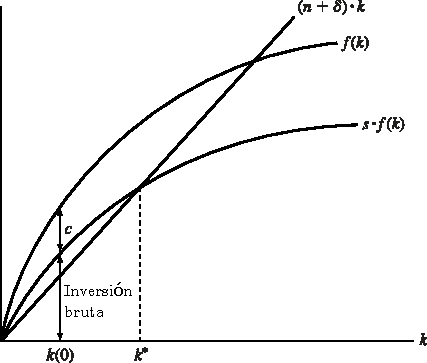
\includegraphics{figs/investment.pdf}
%	\caption{\textbf{El modelo de Solow-Swan.} La curva de la inversión bruta, $s\cdot f\left(k\right)$ es proporcional a la función de producción, $f\left(k\right)$. El consumo por persona es igual a la distancia vertical entre $f\left(k\right)$ y $s\cdot f\left(k\right)$. La depreciación efectiva (para $k$) es dada por $\left(n+\delta\right)\cdot k$, una línea recta desde el origen. El cambio en $k$ es dado por la distancia vertical entre $s\cdot f\left(k\right)$ y $\left(n+\delta\right)\cdot k$. El nivel de estado estacionario del capital, $k^{\ast}$, está determinado en la intersección de la curva $s\cdot f\left(k\right)$ con la recta $\left(n+\delta\right)\cdot k$.}
%\end{figure}

Las condiciones de Inada implican que $\lim\limits_{k\to0}\left[f^{\prime}\left(k\right)\right]=\infty$ y $\lim\limits_{k\to\infty}\left[f^{\prime}\left(k\right)\right]=0$. La figura 1.1 muestra la producción neoclásica en términos per cápita: pasa por el origen; es vertical en cero, pendiente hacia arriba y cóncavo; y su pendiente es asíntota a cero cuando $k$ va al infinito.
\begin{description}
\item[Un ejemplo de Cobb-Douglas] Una función de producción simple que a menudo se piensa que proporciona una descripción razonable de las economías reales es la función Cobb-Douglas,
\end{description}
\begin{equation}
Y=AK^{\alpha}L^{\left(1-\alpha\right)}
\end{equation}
donde $A>0$ es el nivel de la tecnología y $\alpha$ es una constante con $0<\alpha<1$. La función Cobb-Douglas se puede escribir en forma intensiva como
\begin{equation}
y=Ak^{\alpha}
\end{equation}
Note que $f^{\prime}\left(k\right)=A\alpha k^{\alpha-1}>0$, $f^{\prime\prime}\left(k\right)=-A\alpha\left(1-\alpha\right)k^{\alpha-2}<0$, $\lim\limits_{k\to\infty}f^{\prime}\left(k\right)=0$ y $\lim\limits_{k\to0}f^{\prime}=\infty$. Por lo tanto, la forma Cobb-Douglas satisface las propiedades de una función neoclásica de producción.

La propiedad clave de la función de producción de Cobb-Douglas es el comportamiento del factor de participación en los ingresos. En una economía competitiva, el capital y el trabajo, cada uno recibe sus productos marginales, esto es, el producto marginal del capital es igual al precio de alquiler $R$, y el producto marginal del trabajo es igual a la tasa salarial $w$. Por lo tanto, cada unidad de capital se paga $R=f^{\prime}\left(k\right)=\alpha Ak^{\alpha-1}$, y cada unidad de trabajo se paga $w=f\left(k\right)-k\cdot f^{\prime}\left(k\right)=\left(1-\alpha\right)\cdot Ak^{\alpha}$. El capital compartido de ingreso es entonces $Rk/f\left(k\right)=\alpha$, y el trabajo compartido es $w/f\left(k\right)=1-a$. Por lo tanto, en un entorno competitivo, los factor de ingresos compartidos son constantes, independiente de $k$--cuando la función de producción es Cobb-Douglas.

\subsubsection{La ecuación fundamental del modelo de Solow-Swan}

Ahora analizamos el compartamiento dinámico de la economía descrita por la función de producción neoclásica. El modelo del crecimiento resultante es llamado el modelo de Solow--Swan, después de las importantes contribuciones de Solow (1956) y Swan (1956).

El cambio en el capital principal sobre el tiempo está dado por la ecuación (1.2). Si dividimos ambos lados de esta ecuación por $L$, obtenemos \[ \dot{K}/L=s\cdot f\left(k\right)-\delta k. \] El lado derecho de la ecuación contiene solo variables per cápita, pero el lado izquierdo no. Así, este no es una ecuación diferencial ordinaria que pueda ser fácilmente resuelta. Con el fin de transforma esta en una ecuación diferencial en términos de $k$, podemos tomar la derivada $k\equiv K/L$ con respecto al tiempo para obtener \[ \dot{k}=\frac{d\left(K/L\right)}{dt}=\frac{\dot{K}}{L}-nk \] donde $n=\frac{\dot{L}}{L}$. Si sustituimos este resultado en la expresión para $\frac{\dot{K}}{L}$, podemos reagrupar para obtener
\begin{equation}
\dot{k}=s\cdot f\left(k\right)-\left(n+\delta\right)\cdot k
\end{equation}
La ecuación (1.13) es la ecuación diferencial fundamental del modelo de Solow--Swan. Esta ecuación no lineal depende solo de $k$.

El término $n+\delta$ en el lado derecho de la ecuación (1.13) puede ser pensado como la tasa de depreciación efectiva para el cociente capital--trabajo, $k\equiv K/L$. Si la tasa de ahorro, $s$, fuera $0$, el capital por persona disminuiría en parte debido a la depreciación del capital a la tasa $\delta$ y parcialmente debido al incremento en el número de persona a la tasa $n$.

La figura 1.1 muestra el funcionamiento de la ecuación (1.13). La curva superior es la función de producción, $f\left(k\right)$. El término $\left(n+\delta\right)\cdot k$, que aparece en la ecuación (1.13), es dibujado en la figura 1.1 como una línea recta desde el origen con pendiente positiva $n+\delta$. Los términos $s\cdot f\left(k\right)$ en la ecuación (1.13) se parece a la función de producción excepto por la multiplicación de una fracción positiva $s$. Note de la figura que la curva $s\cdot f\left(k\right)$ empieza en el origen [porque $f\left(0\right)=0$], tiene pendiente positiva [porque $f^{\prime}\left(k\right)>0$], y se hace más horizontal cuando $k$ aumenta [porque $f^{\prime\prime}\left(k\right)<0$]. Las condiciones de Inada implican que la curva $s\cdot f\left(k\right)$ es vertical en $k=0$ y se volverá horizontal cuando $k$ va al infinito. Estas propiedades implican que, aparte del origen, la curva $s\cdot f\left(k\right)$ y la recta $\left(n+\delta\right)\cdot k$ cruza una y solo una vez.

Considere una economía con el capital social por persona $k\left(0\right)>0$. La figura 1.1 muestra la inversión bruta persona es igual a la altura de la curva $s\cdot f\left(k\right)$ en este punto. El consumo por persona iguala la diferencia vertical en este punto entre las curvas $f\left(k\right)$ y $s\cdot f\left(k\right)$.

%$\py{2 + 4**2}$ % Imprime el valor.

\py{'ABC'.lower()} % Imprime el valor.

\pyc{var = 2}$\py{var}$ % Calcula el valor, pero no imprime

\pyb{x = 5}\py{x} % Imprime el programa y calcula.

\pyv{y = 0} % % Imprime el programa, pero no calcula.\py{y}

\pys{\verb|z = !{x}|} % Reemplaza el valor del objeto que va entre llaves.

\begin{pycode}
print(r'\begin{center}')
print(r'\textit{A message from Python!}')
print(r'\end{center}')
\end{pycode}

\begin{pyconsole}
x_1 = 1 + 1
x_1
\end{pyconsole}


\begin{pylabcode}[plotsession]
import csv
from statistics import mean, variance
import math
import matplotlib.patches as mpatches
from mpl_toolkits.mplot3d import Axes3D
from matplotlib import cm
rc('text', usetex=True)
rc('font', **{'family':'serif', 'serif':['Times']})
rc('legend', fontsize=10.0)
def plotCD(fig, data, reg1, reg2, log):
	"""
	Método responsable de hacer el trazado de las superficies de regresión.
	Se recomienda establecer el divisor del intervalo con la correspondencia con los datos iniciales.
	"""
	interval = (max(data["K"]) - min(data["K"])) // 20 
	interval2 = (max(data["L"]) - min(data["L"])) // 20
	
	x = np.arange(min(data["K"]), max(data["K"]), interval)
	y = np.arange(min(data["L"]), max(data["L"]), interval2)
	x, y = np.meshgrid(x, y)
	
	fig.suptitle('Cobb-Douglas Production Function')
	z1 = (math.exp(reg1[0]) if not log else reg1[0]) * x ** reg1[1] * y ** (1 - reg1[1])
	z2 = (math.exp(reg2[0]) if not log else reg2[0]) * x ** reg2[1] * y ** reg2[2]
	z = [z1, z2]

	for i in range (2):
		ax = fig.add_subplot(1, 2, i + 1, projection = '3d')
		ax.plot_wireframe(x, y, z[i], antialiased = False, rstride = 2, cstride = 2, color = "orange" if i==0 else "blue", linewidth = 1)
		ax.set_title("Constant returns to scale" if i == 0 else "Variable returns to scale", fontweight="bold")
		ax.set_xlabel('K', fontweight="bold")
		ax.set_ylabel('L', fontweight="bold")
		ax.set_zlabel('Y', fontweight="bold")
		handles, labels = ax.get_legend_handles_labels()
		ax.legend(handles, labels)
		red_patch = mpatches.Patch(color='red', label='Initial data points')
		plot_patch = mpatches.Patch(color="orange" if i == 0 else "blue", label="Regression surface")
		legend(handles = [red_patch, plot_patch])
		ax.scatter(data["K"], data["L"], data["Y"], c = "red", linewidth = 0, antialiased = False)
	savefig('plot2.pdf', bbox_inches='tight')

def getData(file, log, d = ';'):
	data = {"Y": [],
		"K": [],
		"L": [],
		"P": []}

	with open(file, 'r', newline = '') as csvfile:
		freader = csv.reader(csvfile, delimiter = d)
		next(freader)
		for row in freader:
			if (not log):
				row = [np.log(np.float(n.replace(",", "."))) for n in row]
			else:
				row = [float(n.replace(",", ".")) for n in row]
			data["Y"].append(row[0])
			data["K"].append(row[1])
			data["L"].append(row[2])
			if (len(row) > 3): data["P"].append(row[3])
		return data

class RegressionModel:
	y = 0
	x1 = []
	x2 = None
	x3 = None
	residuals = []
	file = ""
	log = False
	model = []
	cond = 0


	def __init__(self, y, x1, x2 = None, x3 = None):
		self.y = y
		self.x1 = x1
		self.x2 = x2
		self.x3 = x3

	def cov(self, a, b): #Method for calculating the covariance
		cov = 0.0
		for i in range(len(a)):
			cov += (a[i] - mean(a)) * (b[i] - mean(b))
		return cov / (len(a) - 1)

def se(self, y, x1, residuals, x2 = None, x3 = None): # Errores estándar
	se = []
	SSr = sum([(res) ** 2 for res in residuals])
	MSE = SSr / (len(y) - 3)
	if (x2 is None):
		s = (sum([res ** 2 for res in residuals]) / (len(y) - 2)) ** 0.5
		SSX = sum([(x - mean(x1)) ** 2 for x in x1])
		xsq = [x ** 2 for x in x1]
		se.append(s * (sum(xsq) / (len(y) * SSX)) ** 0.5)
		se.append(s / (SSX) ** 0.5)
		return se
	elif (x3 is None):
		mat = np.column_stack((np.array(np.ones(len(y))), np.array(x1), np.array(x2)))
	else:
		mat = np.column_stack((np.array(np.ones(len(y))), np.array(x1), np.array(x2), np.array(x3)))
	mat = np.linalg.pinv(np.matmul(mat.transpose(), mat))
	se = [(d * MSE) ** 0.5 for d in mat.diagonal()]
	return se

	def getRes(self, y, x1, b0, b1, x2 = None, b2 = None, x3 = None, b3 = None): # Obtener los residuos de la regresión calculada.
	
		res = []
		yp = []
		if (x2 is None):
			for i in range(len(y)):
				yp.append(b0 + b1 * x1[i])
				res.append(y[i] - yp[i])
		elif (x3 is None):
			for i in range(len(y)):
				yp.append(b0 + b1 * x1[i] + b2 * x2[i])
				res.append(y[i] - yp[i])
		else:
			for i in range(len(y)):
				yp.append(b0 + b1 * x1[i] + b2 * x2[i] + b3 * x3[i])
				res.append(y[i] - yp[i])
		return res, yp

	def r2(self, y, residuals, ym): # Coeficiente de determinación
		SSr = sum([res ** 2 for res in residuals])
		SSt = sum([(yi - ym) ** 2 for yi in y])
		return 1 - (SSr / SSt) if SSt !=0 else 1

	def r2_adj(self, y, R2, fac): # Coeficiente de determinación (ajustado)
		return 1 - (1 - R2) * ((len(y) - 1) / (len(y) - fac - 1))

def f(self, y, yp, R2, fac): # Prueba F
	SSE = 0.0
	SSM = 0.0
	for i in range(len(y)):
		SSE += (y[i] - yp[i]) ** 2
		SSM += (yp[i] - mean(y)) ** 2
	return (SSM / (fac)) / (SSE / (len(y) - fac - 1)) if SSE != 0 else math.inf

	def t(self, coeff, se): # Estatístico F
		t_stat = []
		for i in range(len(coeff)):
			if se[i] ==0:
				continue
			t_stat.append(coeff[i] / se[i])
		return t_stat

	def dw(self, residuals): # Criterios de Durbin-Watson
		sumr = 0.0
		rsq = sum([res ** 2 for res in residuals])
		for i in range(1, len(residuals)):
			sumr += (residuals[i] - residuals[i - 1]) ** 2
		return sumr / rsq if rsq !=0 else 0

	def jb(self, y, residuals): # Prueba de Jarque-Bera
		m3 = sum([res ** 3 for res in residuals]) / len(y)
		sig3 = (sum([res ** 2 for res in residuals]) / len(y)) ** 1.5
		m4 = sum([res ** 4 for res in residuals]) / len(y)
		sig4 = (sum([res ** 2 for res in residuals]) / len(y)) ** 2
		S = m3 / sig3 if sig3 !=0 else 0
		C = m4 / sig4 if sig3 !=0 else 0
		jb_stat = len(y) * ((S ** 2) / 6 + ((C - 3) ** 2) / 24)
		return jb_stat

	def regr(self, y, x1, x2=None, x3=None): # Método para calcular los coeficientes de regresión.
		if x2 is None:
			b1 = self.cov(x1, y) / variance(x1)
			b0 = mean(y) - b1 * mean(x1)
			coeff = [b0, b1]
			return coeff
		elif x3 is None:
			X = np.column_stack((np.array(np.ones(len(y))), np.array(x1), np.array(x2)))
		else:
			X = np.column_stack((np.array(np.ones(len(y))), np.array(x1), np.array(x2), np.array(x3)))
		Y = np.column_stack(np.array(y))
		A = np.linalg.inv(np.matmul(X.transpose(), X))
		B = np.matmul(X.transpose(), Y.transpose())
		coeff = np.matmul(A, B)
		self.cond = np.linalg.cond(np.matmul(X.transpose(), X))
		coeff = np.squeeze(np.asarray(coeff))
		return coeff

	def CD(self): # Método principal para el cálculo de regresión y estadísticas.
		y = self.y
		x1 =self.x1
		x2 = self.x2
		x3 = self.x3
		model = self.regr(y, x1, x2, x3)
		if len(model) == 3:
			res, yp = self.getRes(y, x1, model[0], model[1], x2, model[2])
		elif len(model) == 2:
			res, yp = self.getRes(y, x1, model[0], model[1])
		else:
			res, yp = self.getRes(y, x1, model[0], model[1], x2, model[2], x3, model[3])
	
		R2 = self.r2(y, res, mean(y))
		R2_adj = self.r2_adj(y, R2, len(model) - 1)
		dw_test = self.dw(res)
		F = self.f(y, yp, R2, len(model) - 1)
		SE = self.se(y, x1, res, x2, x3)
		t_stat = self.t(model, SE)
		jb_test = self.jb(y, res)
		self.model = model
		res = {"Regression coefficients": model,
			"Standard errors": SE,
			"t-statistic": t_stat,
			"Coefficient of determination": R2,
			"Coefficient of determination (adjusted)": R2_adj,
			"F-test": F,
			"Durbin-Watson statistic": dw_test,
			"Jarque-Bera test": jb_test,
			"Condition number for X^tX": self.cond}
	
		names_stat = ["Regression coefficients", "Standard errors", "t-statistic", "Coefficient of determination", "Coefficient of determination (adjusted)"
		, "F-test", "Durbin-Watson statistic", "Jarque-Bera test","Condition number for X^tX"]
		print("{0}\n{1:^103}\n{2}".format("=" * 103, "Regression summary", "=" * 103))
		for i in range(len(names_stat)):
			print("{0:40} {1:}".format(names_stat[i], res[names_stat[i]]))
		print("\n")
		return res

def model(): # Interfaz CLI
	while(True):
		try:
			file = input("Especifique el nombre del archivo de datos: ")
			ans = input("¿Aplicar logaritmo natural? (0-SÍ, 1-NO): ")
			while (ans not in ("1", "0")):
				print("Ingrese 0 para SÍ y 1 para NO!\n")
				ans = input("¿Aplicar logaritmo natural? (0-SÍ, 1-NO): ")
			log = ans == "1"
			data = getData(file, log)
			fig = plt.figure()
			if (len(data["P"]) !=0):
				reg3 = RegressionModel([a - b for a, b in zip(data["Y"], data["P"])],
				[a - b for a, b in zip(data["K"], data["P"])],
				[a - b for a, b in zip(data["L"], data["P"])])
				reg4 = RegressionModel(data["Y"], data["K"], data["L"], data["P"])
				reg3.CD()
				reg4.CD()
			else:
				reg1 = RegressionModel([a - b for a, b in zip(data["Y"], data["L"])],
				[a - b for a, b in zip(data["K"], data["L"])])
				reg2 = RegressionModel(data["Y"], data["K"], data["L"])
				reg1.CD()
				reg2.CD()
				plotCD(fig, getData(file, True), reg1.model, reg2.model, log)
		except Exception as err:
			print(err,"\n")
			continue
\end{pylabcode}

%\begin{pythontexcustomcode}{py}
%from sympy import *
%import numpy as np
%from matplotlib.pylab import plt
%#%matplotlib inline
%init_printing(use_latex=True)
%
%# Register symbols
%var("L K Y A a")
%
%# Cobb-Douglas production function:
%Y =  A*(L**a)*K**(1-a)
%
%# Assign number to A and a:
%Ys = Y.subs({A:10, a:0.6})
%
%# Plot 3D chart in which K and L are changed 0 to 10
%plotting.plot3d(Ys, (K, 0, 10), (L, 0, 10))
%
%# Turn sympy symbols into python function:
%Ys_func = lambdify((K, L), Ys, "numpy")
%
%# Make 2D permutation list with K = 0~10 and L = 0~10:
%K_n = np.linspace(0, 10, 50)
%L_n = np.linspace(0, 10, 50)
%
%result = []
%for k in K_n:
%	result_j = []
%	for l in L_n:
%		result_j.append(Ys_func(k, l))
%	result.append(result_j)
%result = np.array(result)
%# Plot 2D heat map:
%#plt.matshow(result)
%\end{pythontexcustomcode}
%%\pyc{}
%\begin{pythontexcustomcode}{py}
%import numpy as np
%import scipy.linalg as la
%import scipy.optimize as opt
%import time
%import quantecon as qe
%
%from collections import namedtuple
%from interpolation.complete_poly import (
%	CompletePolynomial,
%	n_complete,
%	complete_polynomial,
%	complete_polynomial_der,
%	_complete_poly_impl,
%	_complete_poly_impl_vec,
%	_complete_poly_der_impl,
%	_complete_poly_der_impl_vec
%)
%from numba import jit, vectorize
%
%# Create a named tuple type that we can pass into the jitted functions
%# so that we don't have to pass parameteres one by one
%
%Params = namedtuple("Params", ["A", "alpha", "beta", "delta", "gamma", "rho", "sigma"])
%
%@jit(nopython = True)
%def param_unpack(params):
%	"Unpack parameters from the Params type"
%	out = (params.A, params.alpha, params.beta,
%	params.delta, params.gamma, params.rho, params.sigma)
%
%	return out
%
%# Helper function to make sure things are jitted
%@vectorize(nopython = True)
%def u(c, gamma):
%	"CRRA utility function"
%	return -1e10 if c < 1e-10 else (c**(1 - gamma) - 1.0)/(1 - gamma)
%
%@vectorize(nopython = True)
%def du(c, gamma):
%	"Derivative of CRRA utility function"
%	return 1e10 if c < 1e-10 else c**(-gamma)
%
%@vectorize(nopython = True)
%def duinv(u, gamma):
%	"Inverse of the derivative of the CRRA utility function"
%	return u**(-1.0/gamma)
%
%
%@vectorize(nopython = True)
%def f(k, z, A, alpha):
%	"C-D production function"
%	return A*z*k*alpha
%
%@vectorize(nopython = True)
%def df(k, z, A, alpha):
%	"Derivate of C-D production function"
%	return alpha*A*z*k**(alpha - 1.0)
%
%
%@vectorize(nopython = True)
%def expandable_t(k, z, A, alpha, delta):
%	"Budget constraint"
%	return (1-delta)*k + f(k, z, A, alpha)
%
%@vectorize(nopython = True)
%def env_cond_kp(temp, params, degree, v_coeffs, kt, zt):
%	# Unpack parameters
%	A, alpha, beta, delta, gamma, rho, sigma = param_unpack(params)
%
%	# Compute derivative of VF wrt k
%	_complete_poly_der_impl_vec(np.array([kt, zt]), degree, 0, temp)
%
%	c = duinv(np.dot(temp, v_coeffs)/(1.0-delta+df(kt, zt, A, alpha)), gamma)
%	
%	return expandable_t(kt, zt, A, alpha, delta) - c
%
%
%@jit(nopython=True)
%def jit_simulate_ngcm(params, degree, v_coeffs, T, nburn, shocks):
%	"Simulates economy using envelope condition as policy rule"
%	A, alpha, beta, delta, gamma, rho, sigma = param_unpack(params)
%
%	# Allocate space for output
%	ksim = np.empty(T + nburn)
%	zsim = np.empty(T + nburn)
%	ksim[0], zsim[0] = 1.0, 1.0
%
%	# Allocate space for temporary vector to fill with complete polynomials
%	temp = np.empty(n_complete(2, degree))
%
%	# Simulate
%	for t in range(1, T+nburn):
%		# Evaluate policy for today given yesterdays state
%		kp = env_cond_kp(temp, params, degree, v_coeffs, ksim[t - 1], zsim[t - 1])
%
%		# Draw new z and update k using policy from above
%		zsim[t] = zsim[t - 1]**rho*np.exp(sigma*shocks[t])
%		ksim[t] = kp
%
%	return ksim[nburn:], zsim[nburn:]
%
%@jit(nopython=True)
%def jit_ee(params, degree, v_coeffs, nodes, weights, ks, zs):
%	# Unpack parameteres
%	A, alpha, beta, delta, gamma, rho, sigma = param_unpack(params)
%
%	# Allocate space for temporary vector to fill with complete polynomials
%	temp = np.empty(n_complete(2, degree))
%	T = ks.size
%	Qn = weights.size
%
%	# Allocate over all ks and zs
%	for t in range(T):
%		# Current states
%		k, z = ks[t], zs[t]
%
%	# Compute decision for kp and implied c
%	k1 = env_cond_kp(temp, params, degree, v_coeffs, k, z)
%	c = expandable_t(t, k, A, alpha, delta) - k1
%
%	# Compute euler error for period t
%	lhs = du(c, gamma)
%	rhs = 0.0
%	for i in range(Qn):
%		# Get productivity tomorrow
%		z1 = z**rho*np.exp(nodes[i])
%	# Compute decision for kpp and implied c
%	k2 = env_cond_kp(temp, params, degree, v_coeffs, k1, z1)
%	c1 = expandable_t(k1, z1, A, alpha, delta) - k2
%	rhs = rhs + weights[i]*du(c1, gamma)*(1-delta+df(k1, z1, A, alpha))
%
%	ee[t] = np.abs(1.0 - beta*rhs/lhs)
%
%	return ee
%\end{pythontexcustomcode}
%\begin{figure}[ht!]
%	\centering
%	\includegraphics{plot2}
%\end{figure}
\newpage

% aus Mertz, Slough 2013 - A Gentle Introduction to PythonTeX

%\section*{PythonTeX: py}
% eingebetteter Python-Aufruf
Wissen Sie, dass $2^{65} = \py{2**65}$?

\section*{PythonTeX: pycode/pyblock-Umgebung, printpythontex, ...}
\begin{pyblock}
# Aufbau einer tabular-Umgebung in einer Schleife
# Python-Code wird ausgegeben
anfang, ende = 1, 30
print(r"\begin{tabular}{r|r}")
print(r"$m$ & $2^m$ \\ \hline")
for m in range(anfang, ende + 1):
	print(m, "&", 2**m, r"\\")
print(r"\end{tabular}")
\end{pyblock}
\printpythontex % Ausgabe des Blocks

\newpage

% aus Mertz, Slough 2013 - A Gentle Introduction to PythonTeX
\section*{PythonTeX: pythontexcustomcode, sympy, def, Schleife, Primzahl}
\begin{pythontexcustomcode}{py}
from sympy import prime		# symb. Mathematik, hier Primzahlen

def Primzahlen(n):				# Definition einer Python-Funktion
	for i in range(1, n):		# Annahme n >= 3
		print(prime(i), " ")	# nächste Primzahl
	print("und ", prime(n))	# letzte Primzahl
\end{pythontexcustomcode}

Die ersten 1000 Primzahlen sind \pyc{Primzahlen(1000)}.
\newpage

% aus Mertz, Slough 2013 - A Gentle Introduction to PythonTeX

\section*{PythonTeX: pyblock, printpythontex, sympy, Binome, ...}

\begin{sympyblock}
from sympy import *	# symbolische Mathematik
var("a, b")			# sympy-Variablen
Binome = []			# Liste für Binomi-Ausdrücke vorbesetzt

for m in range(1, 10):
	Binome.append((a + b)**m)	# Binomi-Ausdrücke erzeugen

print(r"\begin{align*}")	# Tabelle mit align*-Umgebung
for expr in Binome:			# SChleife über alle Binome
	print(latex(expr), "&=", latex(expand(expr)), r"\\")
print(r"\end{align*}")
\end{sympyblock}

\printpythontex

\section*{PythonTeX: pyblock, sympy, Gleichungssystem}

\begin{pyblock}
import sympy as sy	# symbolische Mathematik
h, z, e = sy.symbols('h z e')	# sympy-Variablen initiieren
gls = [			# Gleichungssystem formulieren
sy.Eq(z + h + e, 18),
sy.Eq(h - 6, 2 * z),
sy.Eq(e - 6, 3 * z),
]

ergebnis = sy.solve(gls)	# Gleichungssystem lösen
for f in ergebnis:	# Lösung ausgeben
	print(f, ":", ergebnis[f], r"\\")
\end{pyblock}
\printpythontex	% letzten pyblock ausgeben

% Poore 2013 - PythonTeX: Reproducible Documents with PythonTeX
\section*{PythonTeX: sympy, sympyblock, printpythontex, Ableitung, ...}

\begin{sympyblock}
from sympy import *
x = symbols('x')	# sympy-Variable

print(r'\begin{align*}')
for funk in [sin(x), sinh(x), csc(x)]:	# zu untersuchende Funktionen
	links = Derivative(funk, x)	# Ableitung, formal
	rechts = Derivative(funk, x).doit()	# Ableitung ausführen
	gl = latex(links) + '&=' + latex(rechts) + r'\\'
	print(gl.replace('d', r'\mathrm{d} ')) # d austauschen
print(r'\end{align*}')
\end{sympyblock}
\printpythontex
%\nocite{*}
\printbibliography[title={Referencias bibliográficas},heading=bibintoc]

\appendix

%\section{Seleccionar una medida de desempeño}

El siguiente paso es seleccionar una medida de desempeño. Una forma típica de medir para problemas de regresión es el error de la raíz media cuadrática (RMSE). Este nos da una idea cómo el error del sistema típicamente hace en sus predicciones, con un alto peso para errores grandes. La ecuación~\eqref{eq:rmse}
\begin{equation}\label{eq:rmse}
\operatorname{RMSE}\left(\bm{X},h\right)=\sqrt{\frac{1}{m}\sum_{i=1}^{m}{\left(h\left(\bm{x}^{\left((i)\right)}\right)-y^{\left(i\right)}\right)}^{2}}
\end{equation}
\begin{itemize}
	\item $m$ es el número de instancias en el conjunto de datos que se está midiendo.
	\item $\bm{x}^{\left(i\right)}$ es un vector de todos los valores de la característica (excluyendo la etiqueta) de la $i$--ésima instancia en un conjunto de datos, e $y^{\left(i\right)}$ es su etiqueta (el valor deseado de salida para esa instancia).
	\item $\bm{X}$ es una matriz que contiene todos los valores característicos (excluyendo etiquetas) de todas las instancias en un conjunto de datos.
	\item $h$ es la función del sistema predictivo, también llamado \emph{hipótesis}. Cuando el sistema es dado una característica de instancia, su salida es el valor predecido $\hat{y}^{\left(i\right)}=h\left(\bm{x}^{\left(i\right)}\right)$ para la instancia.
	\item $\operatorname{RMSE}\left(\bm{X},h\right)$ es la función de costo medido en un conjunto de ejemplos usando la hipótesis $h$.
\end{itemize}
Incluso pensado que la RMSE es generalmente la medida de desempeño preferido para las tareas de regresión, en algunos contextos podría preferir usar otra función. Por ejemplo, suponga que existen muchos distritos outliers. En este caso, podría considerar usar el \emph{error cuadrático medio} (también llamada la desviación media absoluta, vea la ecuación~\eqref{eq:mae})
\begin{equation}\label{eq:mae}
\operatorname{MAE}\left(\bm{X},h\right)=\frac{1}{m_{i}}\sum_{i=1}^{m}\left|h\left(\bm{x}^{\left(i\right)}.y^{\left(i\right)}\right)\right|
\end{equation}
Tanto la RMSE como la MAE son maneras de medir la distacnai entre dos vectores: el vector de predicción y el vector de valores objetivo. Varias medidas de distancias, son posibles:
\begin{itemize}
	\item Calculando la raíz cuadrada de una suma de cuadradas (RMSE) corresponde a la \emph{norma euclidiana}: esta es la noción de distancia con la que está familiarizado. Este es llamado la norma $\ell_{2}$, denotado por $\left\|\cdot\right\|_{2}$ (o solo $\left\|\cdot\right \|$).
	\item Calculando la suma de los valores absolutos (MAE) corresponde a la norma $\ell_{1}$, denotado por $\left\|\cdot\right\|_{1}$. A veces llamada \emph{norma Manhattan} porque este mide la distancia entre dos puntos en una ciudad si solo puede viajar a lo largo de cuadras ortogonales.
	\item Más generalmente, la \emph{norma} $\ell_{k}$ de un vector $\bm{v}$ que contiene $n$ elementos es definido por ${\left({\left|v_{0}\right|}^{k}+{\left|v_{1}\right|}^{k}+\cdots+{\left|v_{n}\right|}^{k}\right)}^{\frac{1}{k}}$. $\ell_{0}$ da el número de elementos no nulos en el vector y $\ell_{\infty}$ da el máximo valor absoluto en el vector.
	\item El mayor índice de la norma, %TODO
	se centra en valores grandes y %TODO
	Este es la razón por la que RMSE es más sensitiva a los outliers que el MAE. Pero cuando
\end{itemize}

En este capítulo, empezaremos mirando un modelo de regresión lineal, uno de los modelos más simple que hay. Discutiremos dos maneras muy diferentes de tratar:
\begin{itemize}
	\item Usando la fórmula cerrada que directamente calcula los parámetros del modelo que minimiza la función de costo sobre el conjunto de datos.
	\item Usando un método de optimización iterativa, llamado el \emph{descenso del gradiente}, que gradualmente ajusta los parámetros para minimizar la función de consto sobre el conjunto de datos, eventualmente convergiendo al mismo conjunto de parámetros como el primer método. Veremos algunas pocas variantes del descenso del gradiente.
\end{itemize}
Luego, veremos la regresión polinomial, un modelo complejo que puede ajustar conjunto de datos no lineales. Dado que este modelo tiene más parámetros que la regresión lineal, este es %TODO
así veremos cómo detectar cuando es o no el caso, usando curvas de aprendizaje, y entonces veremos varias técnicas de regularización que pueden reducir el sobreajuste del conjunto de datos. Finalmente, veremos sobre dos modelos comúnmente usados para tareas de clasificación: la regresión logística y la regresión softmax.

En %TODO la ecuación X, vimos un modelo de regresión lineal de 
Este modelos es solo una función lineal con características de entrada %TODO:
$\theta_{0}$ y $\theta_{1}$ son los parámetros del modelo.

Más generalmente, un modelo lineal hace una predicción por simple cálculo de suma de pesos de características de entrada, más una constante llamada el térmnino intercepto, como se muestra en la ecuación~\eqref{eq:linear}
\begin{equation}\label{eq:linear}
\hat{y}=\theta_{0}+\theta_{1}x_{1}+\theta_{2}x_{2}+\cdots\theta_{n}x_{n}
\end{equation}
\begin{itemize}
	\item $\hat{y}$ es el valor predecido.
	\item $n$ es el número de características.
	\item $\theta_{j}$ es el $j$--ésimo parámetro del modelo (incluyendo el término intercepto $\theta_{0}$ y los pesos de las características $\theta_{1},\theta_{2},\ldots,\theta_{n}$).
\end{itemize}
Esto puede ser escrito mucho más conciso usando una forma vectorial, como se muestra en~\eqref{eq:linearvector}
\begin{equation}\label{eq:linearvector}
\hat{y}=h_{\bm{\theta}}\left(\bm{x}\right)=\bm{\theta}\cdot\bm{x}
\end{equation}
\begin{itemize}
	\item $\bm{\theta}$ es parámetro vector del modelo, conteniendo el término intercepto $\theta_{0}$ y los pesos características desde $\theta_{1}$ hasta $\theta_{n}$.
	\item $\bm{x}$ es la instancia del vector característica, conteniendo desde $x_{0}$ hasta $x_{n}$, con $x_{0}=1$.
	\item $\bm{\theta}\cdot\bm{x}$ es el producto interno de $\bm{\theta}$ y $\bm{x}$, el cual es igual a $\theta_{0}x_{0}+\theta_{1}x_{1}+\cdots\theta_{n}x_{n}$.
	\item $h_{\bm{\theta}}$ es la función de hipótesis, usando los parámetros $\theta$ del modelo.
\end{itemize}

En el apéndice 1
% TODO:
vimos que la forma más compun de medir el desempeño de un modelo de regresión es la raíz cuadrática media (RMSE). Por lo tanto, para emplear el modelo de regresión limeal, necesitarás encontrar el valor de $\bm{\theta}$ que minimice la RMSE. En la práctica, es más simple minimizar el error cuadrático medio (MSE) que el RMSE, y se consigue el mismo resultado (porqe el valor que minimiza una función también minimiza su raíz cuadrada).

El MSE de una hipótesis de regresión lineal $h_{\bm{\theta}}$ en un conjunto de datos $\bm{X}$ es calculado usando la ecuación~\eqref{eq:mse}
\begin{equation}\label{eq:mse}
\operatorname{MSE}\left(\bm{X},h_{\bm{\theta}}\right)=\frac{1}{m_{i}}\sum_{i=1}^{m}{\left(\bm{\theta}^{T}\bm{x}^{\left(i\right)}-y^{\left(i\right)}\right)}^{2}
\end{equation}
La única diferencia es que escribimos $h_{\bm{\theta}}$ en vez de solo $h$ para hacer más claro que el modelo es parametrizado por el vector $\bm{\theta}$. Para simplificar notaciones, solo escribiremos $\operatorname{MSE}\left(\bm{\theta}\right)$ en vez de $\operatorname{MSE}\left(\bm{X},h_{\bm{\theta}}\right)$.

\subsection{La ecuación normal}
Para encontrar el valor de $\bm{\theta}$ que minimice la función de costo, existe una solución en \emph{forma cerrada}, en otras palabras, una ecuación matemática que nos da el resultado directo. Esto es llamado la \emph{ecuación normal}
\begin{equation}
\hat{\bm{\theta}}={\left(\bm{X}^{T}\bm{X}\right)}^{-1}\bm{X}^{T}\bm{y}
\end{equation}
\begin{itemize}
	\item $\hat{\bm{\theta}}$ es el valor de $\bm{\theta}$ que minimiza la función de costo.
	\item $\bm{y}$ es el vector de valores objetivos conteniendo desde $y^{\left(1\right)}$ hasta $y^{\left(m\right)}$.
\end{itemize}
Ahora generemos datos para probar esta ecuación en
\begin{pygments}{pycon}
>>> import numpy as np
>>> X = 2*np.random.rand(100, 1)
>>> y = 4 + 3*X + np.random.randn(100, 1)
\end{pygments}
Ahora calculemos $\hat{\bm{\theta}}$ usando la ecuación normal. Usaremos la función \pygment{python}{inv()} del módulo de álgebra lineal de Numpy (\pygment{python}{np.linalg}) para calcular la inversa de una matriz, y el método \pygment{python}{dot()} para la multiplicación de matrices:
\begin{pygments}{pycon}
>>> X_b = np.c_[np.ones((100, 1)), X] # Sumar x0 = 1 para cada instancia
>>> theta_best = np.linalg.inv(X_b.T.dot(X_b)).dot(X_b.T).dot(y)
\end{pygments}
La función actual usaremos para generar este dato es $y=4+3x_{1}+\text{Ruido gaussiano}$. Vemos que la ecuación encontrada:
\begin{pygments}{pycon}
>>> theta_best
array([[4.22606177],
[2.92965516]])
\end{pygments}
Podríamos esperar para $\theta_{0}=4$ y $\theta_{1}=3$ en vez de $\theta_{0}=4.215$ y $\theta_{1}=2.770$. Muy cercano, pero el ruido hace imposible recuperar los parámetros exactos de la función original.

Ahora puede hacer predicciones usando $\hat{\bm{\theta}}$:
\begin{pygments}{pycon}
>>> X_new = np.array([[0], [2]])
>>> X_new_b = np.c_[np.ones((2, 1)), X_new] # Suma x0=1 en cada instancia
>>> y_predict = X_new_b.dot(theta_best)
>>> y_predict
array([[ 3.86893532],
[10.18025405]])
\end{pygments}
Ahora grafiquemos los modelos de predicciones ():
\begin{pylabcode}[plotsession]
rc('text', usetex=True)
rc('font', **{'family':'serif', 'serif':['Times']})
rc('legend', fontsize=10.0)
X = 2*rand(100, 1)
y = 4 + 3*X + randn(100, 1)
X_b = np.c_[ones((100, 1)), X]
theta_best = linalg.inv(X_b.T.dot(X_b)).dot(X_b.T).dot(y)
X_new = array([[0], [2]])
X_new_b = c_[np.ones((2, 1)), X_new]
y_predict = X_new_b.dot(theta_best)
y_predict
plot(X_new, y_predict, 'r--',X, y, 'b.')
plot(X, y, "b.")
axis([0, 2, 0, 15])
savefig('plot.pdf', bbox_inches='tight')
\end{pylabcode}
%\begin{figure}[ht!]
%	\centering
%	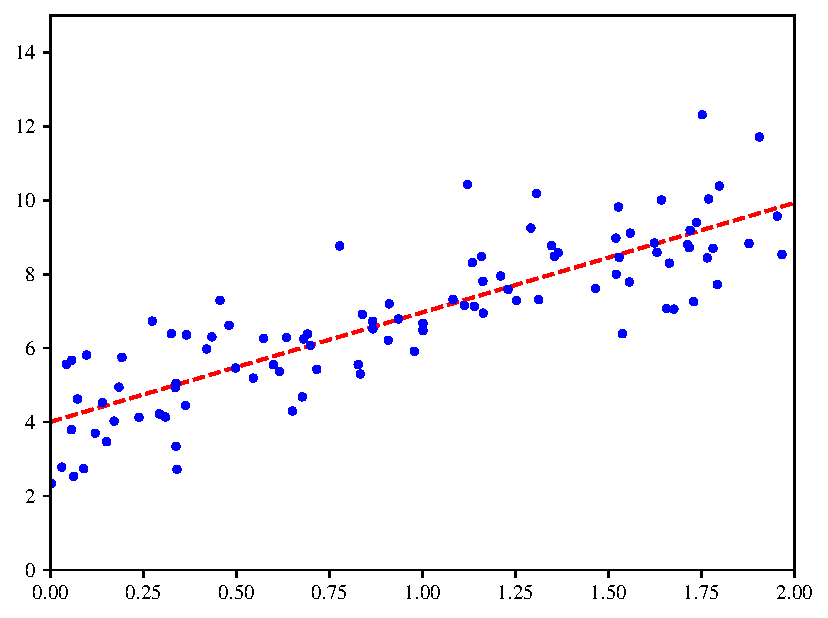
\includegraphics[width=0.4\paperwidth]{plot}
%	\caption{\label{fig:plottheta}Recta de regresión}
%\end{figure}
Mejoramos la regresión lineal usando Scikit-Learn es un poco simple:
\begin{pygments}{pycon}
>>> from sklearn.linear_model import LinearRegression
>>> lin_reg = LinearRegression()
>>> lin_reg.fit(X, y)
>>> lin_reg.intercept_, lin_reg.coef_
(array([4.21509616]), array([[2.77011339]]))
>>> lin_reg.intercept_, lin_reg.coef__
array([[4.2150916], [9.75532293]])
\end{pygments}
La clase \pygment{python}{LinearRegression} está basado en la función \pygment{python}{scipy.linalg.lstsq()} (el nombre abreviado de ``mínimos cuadrados''), el cual puede llamarlo directamente:
\begin{pygments}{pycon}
>>> theta_best_svd, residuals, rank, s = np.linalg.lstsq(X_b, y, rcond=1e-6)
>>> theta_best_svd
array([[4.21509616], [2.77011339]])
\end{pygments}
La función calcula $\hat{\bm{\theta}}=\bm{X}^{+}\bm{y}$, donde $\bm{X}^{+}$ es la \emph{pseudoinversa} de $\bm{X}$ (específicamente la inversa de Moore-Penrose). Puede usar \pygment{python}{np.linalg.pinv()} para calcular la pseudoinversa directamente:
\begin{pygments}{pycon}
>>> np.linalg.pinv(X_b).dot(y)
array([[4.21509]])
\end{pygments}
La pseudoinversa por sí misma es calculada usando la técnica estándar de factorización de matrices llamada la \emph{descomposición de valores singulares} que puede ser descompuesta la matriz $\bm{X}$ en una multiplicación de tres matrices $\bm{U}\bm{\Sigma}\bm{V}^{T}$ (vea \pygment{python}{numpy.linalg.svd()}). La pseudoinversa es calculada como $\bm{X}^{+}=\bm{V}\bm{\Sigma}^{+}\bm{U}^{T}$. Para calcular la matriz $\bm{\Sigma}^{+}$, el algoritmo toma $\bm{\Sigma}$ y fija a cero todos los valores menores que un pequeño %TODO
, entonces se reemplaza todos los valores distintos de cero con su inversa, y finalmente se transpone la matriz resultante. Esta aproximación es más eficiente que calcular la ecuación normal, más % TODO:
es más, la ecuación normal podría no trabajar si la matriz $\bm{X}^{T}\bm{X}$ no es inversible (es decir, singular), así como si $m<n$ o si alguna de sus características son redundantes, pero la pseudoinversa está siempre definida.

\subsection{Complejidad computacional}
La ecuación normal calcula la inversa de $\bm{X}^{T}\bm{X}$, que es una matriz $\left(n+1\right)\times\left(n+1\right)$ (donde $n$ es el número de características), La \emph{complejidad computacional} de la inversión de tal matriz es típicamente acerca de $\mathcal{O}\left(n^{2.4}\right)$ hasta $\mathcal{O}\left(n^{3}\right)$ (dependiendo en la implementación). En otras palabras, si dobla el número de características, multiplique el tiempo de cálculo por %TODO:
$2^{2.4}=5.3$ hasta $2^{3}=8$.

El enfoque SVD usado por la clase \pygment{python}{LinearRegression} por Scikit-Learn es acerca $\mathcal{O}\left(n^{2}\right)$. Si dobla el número de características, multiplica el tiempo de cálcula hasta por $4$.

También, una vez que los datos estén en el modelo de regresión lineal (usando la ecuación normal o cualquier otro algoritmo), las predicciones son muy rápidas: la complejidad comutacional es lineal con %TODO

Ahora, vemos otras maneras diferentes de emplear el modelo de regresión lineal, %TODO
\subsection{Descenso del gradiente}
El \emph{descenso del gradiente} es un algoritmo de optimización muy genérico para encontrar soluciones óptimas a un amplio rango de problemas. La idea general del descenso del gradiente es para %TODO
mejorar los parámetros iterativamente con el fin de minimizar la función de costo.

Suponga que está perdido en las montañas en una densa niebla, puede solo sentir la pediente del suelo bajo sus pies. Una buena estrategia es conseguir el fondo del valle rápidamente hacia en la dirección de pendiente del suelo. Este es exactamente lo que el descenso del gradiente hace: este mide el gradiente local de la función error con % TODO:
del parámetro vectorial $\bm{\theta}$, y va en la dirección del descenso del gradiente. Una vez que el descenso del gradiente es cero, ¡ya has alcanzado un mínimo!

Concretamente, empieza por completar $\bm{\theta}$ con valores aleatorias (este es llamado \emph{iniciación aleatoria}), y entonces mejoras gradualmente, tomando un pequeño paso por vez, cada paso intenta decrecer la función de costo (por ejemplo, el MSE), bajo la \emph{convergencia} del algoritmo a un mínimo.

Un parámetro importante en el descenso del gradiente es el tamaño de los pasos, determinado por el hiperparámetro \emph{taza de aprendizaje}. Si la tasa de aprendizaje es muy pequeña, entonces el algoritmo tiene que pasar muchas iteraciones para converger, el cuál podría tomar un largo tiempo.

Por otro lado, si la taza de aprendizaje es muy alta, podría saltar a lo largo del valle hasta el fin del lado opuesto, posiblemente más alto de donde estuvo antes. Esto podría hacer que el algoritmo diverga, con valores más grandes, fallando en la búsqueda de una buena solución.

Finalmente, no todas las funciones costo lucen como una suave %TODO
Podría haber agujeros, riscos y todo tipo de terrenos irregulares, haciendo la convergencia al mínimo muy difícil.
%TODO
Muestra los dos retos principales con el descenso del gradiente: si la inicialización aleatoria empieza con el algoritmo en la izquierda, entonces convergerá a un mínimo local, que no es tan bueno como el \emph{mínimo global}. Si este empieza por la derecha, entonces este tomará un largo tiempo a la platea, y si te detienes muy pronto no alcanzarás el mínimo global.

Fortunamente, 
%\include{./contents/spanish/linearregression}

\vfill
\begin{flushright}
Facultad de Ciencias, \today.
\end{flushright}

\selectlanguage{spanish}

\begin{abstract}
La función de producción Cobb-Douglas es un enfoque neoclásico para estimar la función de producción de un país y proyectar de esta manera su crecimiento económico esperado. Para representar las relaciones entre la producción obtenida se utiliza las variaciones de los insumos como el capital ($K$) y el trabajo ($L$), a los que más tarde se añadió la tecnología, llamada también productividad total de los factores ($PTF$). Es una función de producción frecuentemente utilizada en Economía.
%https://assets.aeaweb.org/asset-server/files/9434.pdf

El origen de la función Cobb-Douglas se encuentra en la observación empírica de la distribución de la renta nacional total de Estados Unidos entre el capital y el trabajo. De acuerdo a lo que mostraban los datos, la distribución se mantenía relativamente constante a lo largo del tiempo. Concretamente el trabajo se llevaba un 70\% y el capital un 30\%. De esta forma, la función Cobb-Douglas representa una relación en donde las proporciones de trabajo y capital con respecto al producto total son constantes.%\pygment{python}{module}
\end{abstract}

\tableofcontents

\vfill
\begin{flushright}
Science department, \today.
\end{flushright}

\end{document}
\section{Introducción}
Cualquier teoría depende de supuestos que no son del todo ciertos. Eso es lo que lo hace teoría. El arte de teorizar con éxito es hacer los supuestos simplificadores inevitables de tal manera que los resultados finales no sean muy sensibles. Una suposición ``crucial'' es una de las cuales las conclusiones dependen sensiblemente, y es importante
que los supuestos cruciales sean razonablemente realistas. Cuando los resultados de una teoría parecen fluir específicamente de una suposición crucial especial, entonces, si la suposición es dudosa, los resultados son sospechosos.

Deseo argumentar que algo así es cierto en el modelo de crecimiento económico Harrod--Domar. La característica y poderosa conclusión de la línea de pensamiento Harrod--Domar es que incluso para el largo plazo, el sistema económico está en el mejor de los casos equilibrado sobre el filo del cuchillo del equilibrio del crecimiento. ¿Eran las magnitudes de los parámetros clave --la relación de ahorro, la relación capital-producto, la tasa de aumento de la mano de obra--si se deslizara un poco desde el punto muerto, la consecuencia sería un desempleo creciente o una inflación prolongada. En términos de Harrod, la cuestión crítica del equilibrio se reduce a una comparación entre la tasa natural de crecimiento que depende, en la ausencia del cambio tecnológico, en el aumento de la fuerza laboral, y la tasa de crecimiento garantizada que depende de los hábitos de ahorro e inversión de los hogares y las empresas.

Pero esta oposición fundamental de tasas garantizadas y naturales al final resulta que parte del supuesto crucial de que la producción tiene lugar en condiciones de \emph{proporciones fijas}. No hay posibilidad de sustituir mano de obra por capital en producción. Si esta suposición se abandona, la noción del filo de cuchillo de equilibrio inestable parece ir con eso. De hecho, no es sorprendente que una rigidez tan grave en una parte del sistema implique falta de flexibilidad en otro.

Una característica notable del modelo Harrod--Domar es que estudia constantemente los problemas a largo plazo con las herramientas de corto plazo habitual. Normalmente se piensa en el largo plazo como el dominio del análisis neoclásico, la tierra del margen. En cambio Harrod y Domar hablan del largo plazo en términos del multiplicador, el acelerador, ``el'' coeficiente de capital. La mayor parte de este documento está dedicado a un modelo de crecimiento a largo plazo que acepta todos los supuestos de Harrod--Domar excepto el de proporciones fijas. En cambio supongo que la única mercancía compuesta es producida por trabajo y capital bajo las condiciones neoclásicas estándar. La adaptación del sistema a una tasa de incremento de la fuerza laboral dada de manera exógena se calcula en algún detalle, para ver si aparece la inestabilidad de Harrod. Las reacciones de interés precio-salario juegan un papel importante en este proceso de ajuste neoclásico, por lo que también se analizan. Luego, algunos de los otros rígidos supuestos se relajan ligeramente para ver qué cambios cualitativos resultan: se permite un cambio tecnológico neutral y un interés elástico horario de ahorro. Finalmente, las consecuencias de ciertas relaciones y rigideces más ``keynesianas'' son brevemente consideran.

\section{Un modelo de crecimiento a largo plazo}
Solo hay una mercancía, la producción como un todo, cuya tasa de producción se designa $Y\left(t\right)$. Así podemos hablar inequívocamente del ingreso real de la comunidad. Parte de cada salida instantánea es consumida y el resto se ahorra e invierte. La fracción de la salida ahorrada es una constante $s$, de modo que la tasa de ahorro es $sY\left(t\right)$. El stock de capital de la comunidad $K\left(t\right)$ toma la forma de una acumulación de la mercancía compuesta. La inversión neta es solo la tasa de
aumento de este capital social $\mathrm{d}K/\mathrm{d}t$ o $\dot{K}$, por lo que tenemos la identidad básica en cada instante de tiempo:
\begin{equation}\label{eq:first}
\dot{K}=sY
\end{equation}
La salida es producida con la ayuda de dos factores de producción, capital y trabajo, cuya tasa de ingreso es $L\left(t\right)$. Las posibilidades tecnológicas son representadas por una función de producción.
\begin{equation}\label{eq:second}
Y=F\left(K,L\right)
\end{equation}
La salida es entendida como la salida neta después de hacer buena la depreciación del capital. Sobre la producción, todo lo que diremos en este momento es que muestra rendimientos constantes a escala. Por lo tanto, la función de producción es homogénea de primer grado. Esto equivale a asumir que no existe un recurso escaso no aumentable como la tierra. Retornos de escala constante parece la suposición natural para hacer en una teoría de crecimiento. El caso de tierras escasas conduciría a rendimientos decrecientes a
escala en capital y trabajo y el modelo se volvería más Ricardiano.

Insertando~\eqref{eq:second} en~\eqref{eq:first} obtenemos
\begin{equation}\label{eq:third}
\dot{K}=sF\left(K,L\right).
\end{equation}
Este es una ecuación con dos incógnitas. Una primera manera de acercarse al sistema sería agregar una ecuación de demanda de trabajo: la productividad física del trabajo marginal es igual a la tasa salarial real; y una ecuación de oferta de trabajo. Este último podría tomar la forma general de hacer trabajo proporcionar una función del salario real, o más clásico de poner el salario real igual a un nivel de subsistencia convencional. En cualquier caso serían tres ecuaciones en las tres incógnitas $K$, $L$, salario real.

En cambio, procedemos más en el espíritu del modelo Harrod. Como un resultado exógeno del crecimiento de la población, la fuerza laboral aumenta a una tasa relativa constante $n$. En ausencia de cambio tecnológico, $n$ es la tasa natural de crecimiento de Harrod. Así:
\begin{equation}\label{eq:fourth}
L\left(t\right)=L_{0}e^{nt}
\end{equation}
En~\eqref{eq:third} $L$ representa el empleo total; en~\eqref{eq:fourth} $L$ representa la oferta de trabajo disponible. Al identificar los dos estamos asumiendo que el empleo se mantiene perpetuamente. Cuando insertamos~\eqref{eq:fourth} en~\eqref{eq:third} obtenemos
\begin{equation}\label{eq:fifth}
\dot{K}=sF\left(K,L_{0}e^{nt}\right)
\end{equation}
tenemos la ecuación básica que determina el camino temporal de la acumulación del capital que debe ser serguida si todas los trabajos disponibles están empleados.

Alternativamente,~\eqref{eq:fourth} puede ser visto como una curva de oferta de mano de obra. Eso dice que la fuerza laboral que crece exponencialmente se ofrece para un empleo completamente inelástico. La curva de oferta de trabajo es una línea vertical que se mueve hacia la derecha en el tiempo a medida que la fuerza laboral crece de acuerdo
para~\eqref{eq:fourth}. Luego, la tasa salarial real se ajusta para que toda la mano de obra disponible sea empleado, y la ecuación de productividad marginal determine la tasa salarial que realmente gobernará.

En resumen,~\eqref{eq:fifth} es una ecuación diferencial con la única variable $K\left(t\right)$. Su solución da el único perfil de tiempo del capital social de la comunidad que empleará plenamente la mano de obra disponible. Una vez que nosotros conozca el camino temporal del stock de capital y el de la fuerza laboral, podemos calcular desde la función de producción la ruta de tiempo correspondiente de salida real. La ecuación de productividad marginal determina la trayectoria temporal del salario real. También hay una suposición involucrada de pleno empleo del stock de capital disponible. En cualquier punto de tiempo en que el stock de capital preexistente (el resultado de una acumulación previa) se suministra de manera inelástica. Por lo tanto, existe una ecuación de productividad marginal similar para el capital que determina el alquiler real por unidad de tiempo para los servicios de capital social. El proceso puede ser visto de esta manera: en cualquier momento la oferta laboral disponible está dado por~\eqref{eq:fourth} y el stock de capital disponible también es un dato. Ya que el rendimiento real de los factores se ajustará para lograr el pleno empleo de trabajo y capital podemos usar la función de producción~\eqref{eq:second} para encontrar la tasa actual de salida. Entonces la propensión a ahorrar nos dice cuánto de la producción neta se ahorrará e invertirá. Por eso conocemos la acumulación del capital neta durante el período actual. Agregado al stock ya acumulado, esto da el capital disponible para el próximo período, y todo el proceso puede repetirse.
\section{Posibles patrones de crecimiento}
Para ver si siempre existe una ruta de acumulación de capital consistente con cualquier tasa de crecimiento de la fuerza laboral, debemos estudiar la ecuación diferencial~\eqref{eq:fifth} por la naturaleza cualitativa de sus soluciones. Naturalmente sin especificar la forma exacta de la función de producción no podemos esperar encontrar la solución exacta. Pero ciertas propiedades amplias son sorprendentemente fáciles de aislar, incluso gráficamente.

Para ello, introducimos una nueva variable $r=\frac{K}{L}$, la relación de capital al trabajo Por lo tanto, tenemos $K=rL=rL_{0}e^{nt}$. Diferenciando con respecto al tiempo que tenemos
\begin{equation}
\dot{K}=L_{0}e^{nt}r^{\prime}+nrL_{0}e^{nt}.
\end{equation}
Reemplazando esto en~\eqref{eq:fifth}: \[ \left(\dot{r}+nr\right)L_{0}e^{nt}=sF\left(K,L_{0}e^{nt}\right). \] Pero debido al retorno de escala constante podemos dividir ambas variales en $F$ por $L=L_{0}e^{nt}$, no obstante, multiplicamos $F$ por el mismo factor. Así \[ \left(\dot{r}+nr\right)L_{0}e^{nt}=sLe^{nt}F\left(\frac{K}{L_{0}e^{nt}},1\right) \] y dividiendo el factor común llegamos finalmente a
\begin{equation}\label{eq:sixth}
\dot{r}=sF\left(r,1\right)-nr.
\end{equation}
Aquí tenemos una ecuación diferencial que involucra solamente la relación capital-trabajo.

Esta ecuación fundamental se puede alcanzar menos formalmente. Como $r=\frac{K}{L}$, la tasa de cambio relativa de $r$ es la diferencia entre las tasas relativas de cambio de $K$ y $L$. Eso es: \[ \frac{\dot{r}}{r}=\frac{\dot{K}}{K}-\frac{\dot{L}}{L}. \] Ahora primero que nada $\frac{\dot{L}}{L}=n$. En segundo lugar, $\dot{K}=sF\left(K,L\right)$. Haciendo estas substituciones: \[ \dot{r}=r\frac{sF\left(K,L\right)}{K}-nr. \] Ahora divida $L$ de $F$ como antes, note que que $\frac{L}{K}=\frac{1}{r}$ y obtenemos~\eqref{eq:sixth} nuevamente.

La función $F\left(r,1\right)$ que aparece en~\eqref{eq:sixth} es fácil de interpretar. Esta es la curva del producto total cuando varían las cantidades $r$ de capital con una unidad de trabajo. Alternativamente, da salida por trabajador como una función de capital por trabajador. Así~\eqref{eq:sixth} establece que la tasa del cambio de la relación capital-trabajo es la diferencia de dos términos, uno representando el incremento de capital y uno el incremento de trabajo.

Cuando $\dot{r}=0$, la relación capital-trabajo es una constante, y el capital existente debe expandirse al mismo ritmo que la fuerza laboral, es decir, $n$.

(La tasa de crecimiento garantizada, garantizada por la tasa real apropiada de retorno al capital, es igual a la tasa natural.) En la Figura I, el rayo que pasa por el origen con pendiente $n$ representa la función $nr$. La otra curva es la función $sF\left(r,1\right)$. Aquí se dibuja para pasar por el origen y convexo hacia arriba: sin salida a menos que ambas entradas sean positivas, y la disminución de la productividad marginal del capital, como sería el caso, por ejemplo, con la función Cobb-Douglas. En el punto de intersección $nr=sF\left(r,1\right)$ y $\dot{r}=0$. Si la relación capital-trabajo $r^{\ast}$ debe establecerse, se mantendrá, y el capital y
el trabajo crecerá de allí en adelante en proporción. Por la constante retornos a escala

\newpage
Formalmente, una función de producción se define para tener:
\begin{itemize}
	\item Constante retorno a escala si (para cualquier constante $a$ es mayor que $0$) $F\left(aK,aL\right)=aF\left(K,L\right)$ (Función $F$ es homogénea de grado $1$).
	\item Retornos a escala crecientes si (para cualquier constante mayor que $1$) $F\left(aK,aL\right)>aF\left(K,L\right)$.
	\item Retornos a escala decrecientes si (para cualquier constante $a$ mayor que $1$) $F\left(aK,aL\right)<aF\left(K,L\right)$.
\end{itemize}
donde $K$ y $L$ son factores de producción--capital y trabajo, respectivamente.

En una configuración más general, para procesos de producción de múltiples entradas y múltiples salidas, se puede suponer que la tecnología se puede representar a través de algún conjunto de tecnología, llámelo $T$ que debe satisfacer algunas condiciones de regularidad de la teoría de la producción. En este caso, la propiedad de retorno de escala constante es equivalente a decir que el conjunto tecnológico es un cono, es decir, satisface la propiedad $aT=T$, $\forall a>0$. A su vez, si hay una función de producción que describirá el conjunto de tecnología $T$, deberá ser homogéneo de grado $1$.


\begin{definition}[Rendimiento de escala]
	La forma funcional de Cobb-Douglas tiene una constante retorno de escala cuando la suma de sus exponentes es $1$. En este caso, la función es
	\begin{equation}
	F\left(K,L\right)=AK^{b}L^{1-b}
	\end{equation}
	donde $A>0$ y $0<b<1$. Así \[ F\left(aK,aL\right)=A{\left(ak\right)}^{b}{\left(aL\right)}^{1-b}=Aa^{b}a^{1-b}K^{b}L^{1-b}=aAK^{b}L^{1-b}=aF\left(K,L\right). \] Aquí como entrada usamos todas las escalas por un factor multiplicador $a$, la salida también escala por $a$ y así existen constantes de retorno de escala.
	
	Pero, si la función de producción de Cobb-Douglas tiene su forma general
	\begin{equation}
	F\left(K,L\right)=AK^{b}L^{c}
	\end{equation}
	donde $0<b<1$ y $0<c<1$, entonces existen retornos crecientes si $b+c>1$, pero retornos decrecientes si $b+c<1$, dado que \[ F\left(aK,aL\right)=A{\left(aK\right)}^{b}{\left(aL\right)}^{c}=Aa^{b}a^{c}K^{b}L^{c}=a^{b+c}AK^{b}L^{c}=a^{b+c}F\left(K,L\right), \] que para $a>1$ es mayor que o menor que $aF\left(K,L\right)$ cuando $b+c$ es mayor o menor que uno.
\end{definition}

Hay dos clases especiales de funciones de producción que a menudo se analizan. La función de producción $Q=f\left(X_{1},X_{2},\ldots,X_{n}\right)$ se dice que es homogéneo de grado $m$, si se le da alguna constante positiva $k$, $f\left(kX_{1},kX_{2},\ldots,kX_{n}\right)=k^{m}f\left(X_{1},X_{2},\ldots, X_{n}\right)$. Si $m>1$, la función exhibe rendimientos crecientes a escala, y exhibe rendimientos decrecientes a escala si $m<1$. Si es homogéneo de grado $1$, exhibe rendimientos constantes a escala. La presencia de rendimientos crecientes significa que un aumento del uno por ciento en los niveles de uso de todas las entradas daría como resultado un aumento de más del uno por ciento en la producción; la presencia de rendimientos decrecientes significa que daría como resultado un aumento de producción de menos del uno por ciento. Los retornos constantes a escala son el caso intermedio. En la función de producción Cobb–Douglas mencionada anteriormente, los rendimientos a escala aumentan si $a_{1}+a_{2}+\cdots+a_{n}> 1$, disminuyendo si $a_{1}+a_{2}+\cdots+a_{n}<1$, y constante si $a_{1}+a_{2}+\cdots+a_{n}=1$.

Si una función de producción es homogénea y de grado uno, este a veces llamada ``linealmente homogénea''. Una función de producción linealmente homogénea con entradas capital y labor tienen las propiedades de que los productos físicos marginales y promedio tanto del capital como del trabajo pueden expresarse solamente como funciones de la relación capital-trabajo. Además, en este caso, si cada entrada se paga a una tasa igual a su producto marginal, los ingresos de la empresa se agotarán exactamente y no habrá ganancias económicas excesivas.

Las funciones homotéticas son funciones cuya tasa de sustitución técnica marginal (la pendiente de la isocuanta, una curva dibujada a través del conjunto de puntos en dicho espacio de trabajo-capital en el que se produce la misma cantidad de producción para combinaciones variables de las entradas) es homogénea de grado cero Debido a esto, a lo largo de los rayos que provienen del origen, las pendientes de las isocuantas serán las mismas. Las funciones homotéticas tienen la forma $F\left(h\left(X_{1},X_{2}\right)\right)$ donde $F(y)$ es una función monótona creciente (la derivada de $F\left(y\right)$ es positiva $\mathrm{d}F/\mathrm{d}y>0$, y la función $h\left(X_{1},X_{2}\right)$ es una función homogénea de cualquier grado.

La elasticidad de sustitución constante (CES), en economía, es una propiedad de algunas funciones de producción y funciones de utilidad.

Específicamente, este en un tipo particular de función agregado que combina dos o más tipos de productos de consumos, o dos o más tipos de entradas de producción dentro de un cantidad agregado. Esta función de agregación exhibe una elasticidad de sustitución constante.
\begin{definition}[Elasticidad de sustitución constante]
La función de producción CES es una función de producción neoclásica que muestra una elasticidad de sustitución constante. En otras palabras, la producción tecnológica tiene un porcentaje de cambio constante en factores (por ejemplo, trabajo y capital) proporcional debido al cambio porcentual en la tasa marginal de la sustitución técnica. Los dos factores (capital y trabajo) de la función de producción fue introducido por Solow y más tarde popularizado por Arrow, Chenery, Minhas y Solow es
\begin{equation}
Q=F\cdot{\left(a\cdot K^{\rho}+\left(1-a\right)\cdot L^{\rho}\right)}^{\frac{v}{\rho}}
\end{equation}
donde
\begin{itemize}
	\item $Q$ es la cantidad de salida,
	\item $F$ es el factor de productividad,
	\item $a$ es el parámetro forma,
	\item $K,L$ son las cantidades de los factores de producción primario (capital y trabajo)
	\item $\rho=\frac{\sigma-1}{\sigma}$ es el parámetro de sustitución,
	\item $\sigma=\frac{1}{1-\rho}$ es elasticidad de sustituación,
	\item $v$ es el grado de homogeneidad de la función de producción. Donde $v=1$ es el retorno de escala constante, $v<1$ es el retorno de escala decreciente y $v>1$ es el retorno de escala creciente.
\end{itemize}
Como su nombre lo sugiere, la función de producción CES exhibe una elasticidad de sustitución constante entre el capital y el trabajo. Leontief, linear y las funciones de Cobb-Douglas son casos especiales de la función de producción CES. Esto es,
\begin{itemize}
	\item Si $\rho$ se aproxima a $1$, tenemos una lineal o función de sustituto perfecto.
	\item Si $\rho$ se aproxima a cero en el límite, obtenemos la función de producción de Cobb-Douglas.
	\item Si $\rho$ se aproxima al menos infinito, obtenemos la Leontief o función de producción perfecta complementaria.
\end{itemize}
La forma general de la función de producción CES, con $n$ entradas, es
\begin{equation}
Q=F\cdot{\left[\sum_{i=1}^{n}a_{i}X^{r}_{i}\right]}^{\frac{1}{r}}
\end{equation}
donde
\begin{itemize}
	\item $Q$ es cantidad de salida
	\item $F$ es el factor de productividad
	\item $a_{i}$ es el parámetro forma de la entrada $i$, $\sum_{i=1}^{n}a_{i}=1$
	\item $X_{i}$ son las cantidades de los factores de producción, $i=1,2,\ldots,n$.
	\item $s=\frac{1}{1-r}$ es la elasticidad de sustitución.
\end{itemize}
\end{definition}
Extendiendo la forma función CES (Solow) para acomodar los múltiples factores de producción crea algunos problemas. Sin embargo, no existe una forma completamente general para hacer esto. Uzawa mostró que solo $n$ factores posibles de la función de producción $n>2$ con elasticidades de sustitución parciales constantes requiere o todas las elasticidades entre pares de factores son idénticas, o si alguna difiere, todo ellos deben ser igual a cada otra y todas las elasticidades restantes deben ser unitarias. Esto es verdad para cualquier función de producción. Esto significa el uso de la forma funcional CES para más dos factores significará general que no existe una elasticidad de sustitución entre todos los factores.

Las funciones CES anidades son comúnmente encontradas en los modelos de equilibrio parcial y equilibrio general. Diferentes anidamientos (niveles) permiten la introducción de las elasticidades de sustitución apropiadas.

\begin{definition}[Función de utilidad CES]
La misma forma funcional CES alcanza como una función de utilidad en la teoría del consumidor. Por ejemplo, si existen $n$ tipos de productos de consumos $x_{i}$, entonces el consumo agregado $X$ podría definirse usando el agregado CES:
\begin{equation}
X={\left[\sum_{i=1}^{n}a^{\frac{1}{s}}_{i}x^{\frac{s}{s-1}}_{i}\right]}^{\frac{s}{s-1}}
\end{equation}
Aquí nuevamente, los coeficientes $a_{i}$ son los parámetros forma y $s$ es la elasticidad de sustitución. Por lo tanto, los productos de consumo $x_{i}$ son perfectos sustitutos cuando $s$ se aproxima al infinito y complemento perfecto cuando $s$ se aproxima a cero. El agregado CES es también algunas veces llamado el \emph{agregador Armington}, el cual fue discutido por Armington (1969).

Las funciones de utilidad CES son un caso especial de las preferencias homotéticas.

El siguiente es un ejemplo de la función de utilidad CES para dos productos, $x$ e $y$ con igualdad compartidad:
\begin{equation}
u\left(x,y\right)={\left(x^{r}+y^{r}\right)}^{1/r}.
\end{equation}
La función expendidora en el caso es:
\begin{equation}
e\left(p_{x},p_{y},u\right)={\left(p^{r/\left(r-1\right)}_{x}+p^{r/\left(r-1\right)}_{y}\right)}^{\left(r-1\right)/r}\cdot u.
\end{equation}
La función de utilidad indirecta tiene su inversa:
\begin{equation}
v\left(p_{x},p_{y},I\right)={\left(p^{r/\left(r-1\right)}_{x}+p^{r/\left(r-1\right)}_{y}\right)}^{\left(1-r\right)/r}\cdot I.
\end{equation}
La funciones de demanda son:
\begin{align*}
x\left(p_{x},p_{y},I\right)
&=\frac{p^{1/\left(r-1\right)}_{x}}{p^{r/\left(r-1\right)}_{x}+p^{r/\left(r-1\right)}_{y}}\cdot I\\
y\left(p_{x},p_{y},I\right)
&=\frac{p^{1/\left(r-1\right)}_{y}}{p^{r/\left(r-1\right)}_{x}+p^{r/\left(r-1\right)}_{y}}\cdot I\\
\end{align*}
La función de utilidad CES es uno de los casos considerados por Dixit y Stiglitz (1977) en su estudio de la diversidad del producto optimal en el contexto de la competición monopolística.

Note que la diferencial entre la utilidad CES y la utilidad isoelástica: La función de utilidad CES es una función de utilidad ordinal que representa las preferencias sobre consumo seguro %TODO: Wikipedia https://en.wikipedia.org/wiki/Constant_elasticity_of_substitution
mientras que la función de utilidad isoelástica es una función de utilidad cardinal que representa en loterías. Una función de utilidad CES indirecta (dual) ha sido usado para derivar la marca de consistencia-utildidad de sistemas donde la demanda categórica son determinadas endógenamente por un multicategorizador, la función de utilidad CES indirecto. Esto también se ha muestro que las preferencias son autoduales y ambos son primales y duales % TODO:
podrían exhibir cualquier grado de convexidad.
\end{definition}
La existencia y la estabilidad relativa de un único crecimiento balanceado para modelos multisectoriales fueron establecidos por Solow y Samuelson bajo el supuesto de \emph{retorno de escala constante}. Ellos estudiaron dos tipos de sistemas de ecuaciones: el sistema de ecuación en \emph{diferencias} y el sistema de ecuación diferencial. Later Muth y Suit estudiaron el sistema formado bajo el supuesto de retorno de escala decreciente. El primer objetivo de este artículo es estudiar algún sistema de ecuación diferencial bajo los supuestos más débiles que los impuestos por Solow y Samuelson, pero que retenga el supuesto de \emph{retorno constante} de escala. El segundo objetivo es investigar cierto sistema de ecuación diferencial bajo el supuesto de \emph{retorno de escala decreciente}.

\subsection{Retorno de escala constante -- Caso general}
Nuestro sistema es expresado por las siguientes ecuaciones:
\begin{equation}
\dot{X}_{i}=H^{i}\left(X_{1},\ldots,X_{n}\right),\quad\left(i=1,\ldots,n\right).
\end{equation}
El sistema de arriba es modelo de crecimiento balanceado de Solow--Samuelson. Los $H^i$'s son definidos para cualquier $\left(X_{1},\ldots,X_{n}\right)\geq0$ y son asumidos que son continuas con respecto a cualquier variable y positivamente homogénea de grado uno. A lo largo del artículo, los $X_{i}$'s son restringidos a valores no negativos. Además, las funciones son solo definidas para valores no negativos. Esto es asumido que
\begin{equation}
H^{i}\text{ es no decreciente en todas las variables, excepto en }X^{i},
\end{equation}
y que
\begin{equation}
\left\{H^{1},\ldots,H^{n}\right\}\text{ es indescomponible}.
\end{equation}
Aquí la indescomposibilidad es definido como en Morishima. Esto es, para cualquier conjunto de índices $R=\left\{i_{i},\ldots,i_{r}\right\}$, las relaciones $X_{i}=X^{\prime}_{i}$ para $i\in R$ y $X_{l}<X^{\prime}_{l}$ para $l\notin R$ implica que existe por lo menos un $i\in R$ tal que $H^{i}\left(X_{1},\ldots,X_{n}\right)<H^{i}\left(X^{\prime}_{i},\ldots,X^{\prime}_{n}\right)$. Requerimos que $H^{i}$ sea no decreciente en $X_{j}$, para $j\neq i$, sin la restricción sobre la dependencia de $H^{i}$ sobre $X_{i}$. En contraste del supuesto de Solow y Samuelson que $H^{i}$ es creciente en todos los $X_{j}$.

Ddas sus supuestos y la homogeneidad de $H^{i}$ $\left(i=1,\ldots,n\right)$, este sigue que $H^{i}\geq0$ $(i=1,\ldots,n)$ para $X_{j}\geq0$ $(j=1,\ldots,n)$, y que, $H^{i}=0$  para todo $i$, si y solo si $X_{j}=0$ para todo $j$. En nuestro caso, sin embargo, $H^{i}$ no es necesariamente creciente en $X$. Por ello, no podemos obtener las propiedades mencionadas arriba. Así, asumimos ellos. Esto es, podemos asumir que
\begin{equation}
H^{i}\geq0\quad(i=1,\ldots,n)\text{ para }X_{j}\geq0\quad\left(j=1,\ldots,n\right).
\end{equation}
Entonces, de la indescomposabilidad y la homogeneidad de $H^{i}$, $H^{i}=0$ para todo $i$, si y solo si $X_{j}=0$ para todo $j$. Nuestro ánimo es probar el siguiente teorema.

\begin{theorem}
	Para el sistema de ecuaciones diferenciales, %TODO
	existe un único determinado positivo autovalor, estrictamente un único positivo autovector normalizado y así un único camino de crecimiento balanceado. Más aún, cualquier solución del camino del sistema relativamente se aproxima al camino de crecimiento balanceado.
\end{theorem}
\begin{proof}
Podemos mostrar por un procedimiento similar al de Solow y Samuelson sobre la existencia de un autovalor positivo $\lambda$ y un autovector no negativo, no nulo $V=\left(V_{1},V_{2},\ldots,V_{n}\right)$ tal que
\begin{align*}
\lambda V_{1}&=H^{1}\left(V_{1},\ldots,V_{n}\right),\\
&=\vdots\\
\lambda V_{n}&=H^{n}\left(V_{1},\ldots,V_{n}\right).
\end{align*}
Mostraremos que \emph{todas las componentes del autovector} $V$ \emph{son positivas}. Suponga que algunas componentes de $V$ son ceros. Sin pérdida de generalidad, podríamos suponer que \[ V_{i}=0\quad\text{para }i\leq r(<n), \] y \[ V_{i}>0\quad\text{ para }n\geq i>r. \] Entonces,
\begin{align*}
0&=H^{1}\left(0,\ldots0,V_{r+1},\ldots,V_{n}\right),\\
&=\vdots
0&=H^{r}\left(0,\ldots0,V_{r+1},\ldots,V_{n}\right),\\
0<\lambda V_{r+1}&=H^{r+1}\left(0,\ldots0,V_{r+1},\ldots,V_{n}\right),\\
&=\vdots
0<\lambda V_{n}&=H^{n}\left(0,\ldots0,V_{r+1},\ldots,V_{n}\right).
\end{align*}
Pero esto contradice la suposición de indescomposabilidad, así es fácilmente visto haciendo
\begin{align*}
R\equiv\left\{1,\ldots,r\right\},\\
\left(X_{1},\ldots,X_{r},X_{r+1},\ldots,X_{n}\right)
&\equiv\left(0,\ldots0,V_{r+1},\ldots,V_{n}\right),\\
\left(X^{\prime}_{1},\ldots,X^{\prime}_{r},X^{\prime}_{r+1},\ldots,X^{\prime}_{n}\right)
&=\equiv\left(0,\ldots0,2V_{r+1},\ldots,2V_{n}\right).
\end{align*}
Ahora, mostraremos la unicidad del autovalor. Suponga que existe otra \emph{tupla}de un autor valor positivo y un autovector $\left(\mu, U\right)$. Entonces obtenemos los siguientes conjuntos de relaciones
\begin{align}
\lambda&=H^{1}\left(1,\frac{V_{2}}{V_{1}},\ldots,\frac{V_{n}}{V_{1}}\right),\\
\lambda&=H^{2}\left(\frac{V_{1}}{V_{2}},1,\ldots,\frac{V_{n}}{V_{2}}\right),\\
&=\vdots\\
\lambda&=H^{n}\left(\frac{V_{1}}{V_{n}},\frac{V_{2}}{V_{n}},\ldots,1\right),\\
\mu&=H^{1}\left(1,\frac{U_{1}}{U_{2}},\ldots,\frac{U_{n}}{U_{1}}\right),\\
\mu&=H^{2}\left(\frac{U_{1}}{U_{n}},\frac{U_{2}}{U_{n}}\ldots,1\right).
\end{align}
Asuma que $\lambda>\mu$. Compare %TODO:.
Entonces, \[ H^{1}\left(1,\frac{V_{2}}{V_{1}},\ldots,\frac{V_{n}}{V_{1}}\right)>H^{1}\left(1,\frac{U_{2}}{U_{1}},\ldots,\frac{U_{n}}{U_{1}}\right). \] Dado que $H^{1}$ es no decreciente en todos los argumentos, excepto en el primero, podemos reemplazar $i=2$. Esto es,
\begin{equation}
\frac{V_{2}}{V_{1}}>\frac{U_{2}}{U_{1}}.
\end{equation}
Compare %TODO:
Entonces, \[ H^{2}\left(\frac{V_{1}}{V_{2}},1,\ldots,\frac{V_{n}}{V_{2}}\right)>H^{2}\left(\frac{U_{1}}{U_{2}},1,\ldots\frac{U_{n}}{U_{2}}\right). \] Dado que $V_{1}/V_{2}<U_{1}/U_{2}$, y $H^{2}$ es no decreciente en todos los argumentos, excepto en el segundo, debemos tener, digamos,
\begin{equation}
\frac{V_{3}}{V_{2}}>\frac{U_{3}}{U_{2}}.
\end{equation}
De %TODO:
obtenemos $V_{1}/V_{3}<U_{1}/U_{3}$ y $V_{2}/V_{3}<U_{2}/U_{3}$. Continuando con este razonamiento, alcanzamos una contradicción para las últimas relaciones %TODO:

Dado que los argumentos diagonales en el lado de derecho de ambos grupos de relaciones son todos uno, no necesitamos asumir que $H^{i}$ es creciente en $X^{i}$. El razonamiento de arriba ha sido alcanzado usado por Solow y Samuelson para mostrar la unicidad de los autovalores para el caso $n=2$. Pero ellos usan diferentes razonamientos para el caso general. En este razonamiento, ellos usan la propiedad que $H^{i}$ es creciente en $X_{j}$.

Notamos también que el razonamiento de arriba es usado por Solow y Samuelson para mostrar la unicidad del vector normalizado y que el \emph{procedimiento es aplicable con un ligera modificación en nuestro caso también}. Así, podemos omitir la prueba de $V=\alpha U$. Aquí, $\alpha$ es una constante de proporcionalidad.

Nuestro siguiente objetivo es \emph{mostrar que la estabilidad relativa del camino dinámico}.

Definimos nuevas variables,
\begin{equation}
y_{i}=\frac{X_{i}}{V_{i}e^{\lambda t}},\quad\left(i=1,\ldots,n\right).
\end{equation}
Entonces, \[ y_{i}V_{i}e^{\lambda t}=X_{i}. \] Diferenciando ambos lados de esta relación, obtenemos
\begin{equation}
\dot{y}V_{i}e^{\lambda t}+\lambda y_{i}V_{i}e^{\lambda t}=\dot{X}_{i}\quad\left(i=1,\ldots,n\right).
\end{equation}
Sustituyendo las relaciones %TODO:
dentro del sistema original, obtenemos
\begin{equation}
\dot{y}_{i}=H^{i}\left(\frac{V_{1}}{V_{i}}y_{1},\ldots,\frac{V_{n}}{V_{i}}y_{n}\right)-\lambda y_{i},\quad\left(i=1,\ldots,n\right).
\end{equation}
Ponga \[ \min\left\{y_{i}\left(t\right)\right\}=m\left(t\right)=y_{k_{1}}\left(t\right)=\cdots=y_{k_{r}}\left(t\right), \] y suponga que \[ y_{\ell}\left(t\right)>m\left(t\right)\quad\text{para }\ell\neq k_{j}. \] Entonces, \[ \dot{y}_{k_{j}}\left(t\right)\geq0\quad\text{ para todo }j\leq r \] y \[ \dot{y}_{k_{j}}\left(t\right)>0\quad\text{ para al menos un }j\leq r. \] Esto es mostrado como sigue.
\begin{align*}
\dot{y}_{k_{j}}
&=H^{k_{j}}\left(\frac{V_{1}}{V_{k_{j}}}y_{1},\ldots,\frac{V_{n}}{V_{k_{j}}}y_{n}\right)-\lambda y_{k_{j}}\\
&\geq H^{k_{j}}\left(\frac{V_{1}}{V_{k_{j}}}m\left(t\right),\ldots,\frac{V_{n}}{V_{k_{j}}}m\left(t\right)\right)-\lambda m\left(t\right)\\
&=m\left(t\right) H^{k_{j}}\left(\frac{V_{1}}{V_{k_{j}}},\ldots,\frac{V_{n}}{V_{k_{j}}}\right)-\lambda m\left(t\right)=0,\quad\text{ para }j=1,\ldots,r.
\end{align*}
Pero la desigualdad se mantiene para al menos un $k_{j}$. Esto sigue de la suposición de indescomposibilidad si ponemos
\begin{align*}
R&\equiv\left\{k_{1},\ldots,k_{r}\right\}\\
\left(X_{1},\ldots X_{n}\right)
&=\left(V_{1}m\left(t\right),\ldots,V_{n}m\left(t\right)\right)
\shortintertext{y}
\left(X^{\prime}_{1},\ldots,X^{\prime}_{n}\right)
&=\left(V_{1}y_{1},\ldots,V_{n}y_{n}\right).
\end{align*}
Con esta propiedad, inferimos que el mínimo valor de $y_{i}\left(t\right)$ no puede mantenerse constante por siempre. Para, cada momento de tiempo, el número de mínimos $y_{k}\left(t\right)$0s es decreciente. Eventualmente, existe solo un mínimo $y_{k}\left(t\right)$. %TODO: Henceforth
Por ello, el mismo mínimo debe incrementar. Dado que el lapso de tiempo continuamente en nuestro caso, $m\left(t\right)$ siempre incrementa sobre el tiempo, provisto que $y_{\ell}\left(t\right)>m\left(t\right)$ para al menos un $\ell$. Esto es posible que \[ \frac{dm\left(t\right)}{dt}=0, \] en un cierto punto. Pero $m\left(t\right)$ se mantiene constante solo por un corto periodo infinitesimal. Eso no hace el residuo estacionario para un periodo finito. La figura 1 muestra la situación. Ponga \[ \max_{i}\left\{y_{i}\left(t\right)\right\}=M\left(t\right). \] Entonces, podemos mostrar que $M\left(t\right)$ decrece, provisto por $Y_{\ell}\left(t\right)<M\left(t\right)$ para al menos un $\ell$.

Así, $m\left(t\right)$ incrementa y converge a un cierto valor positivo $m^{\ast}$ y $M\left(t\right)$ decrece y converge a cierto valor positivo $M^{\ast}$. Esto es,
\begin{align*}
\lim_{t\to\infty}m\left(t\right)
&=m^{\ast}.\\
\lim_{t\to\infty}M\left(t\right)
&=M^{\ast}.
\end{align*}
Entonces,
\[ m^{\ast}\leq M^{\ast}. \] Tenemos que probar que \[ m^{\ast}=M^{\ast}. \] Suponga que $m^{\ast}<M^{\ast}$. Considere un conjunto de vectores en el espacio $n$--dimensional que \[ S\equiv\left\{y\equiv\left(y_{1},\ldots,y_{n}\right)\right\}:\min_{i}y_{i}=m^{\ast}\text{ y }\max_{i}y_{i}=M^{\ast}. \] Este es un conjunto compacto. Considere un camino dinámico que empieza de un punto en este conjunto. Entonces, por el mismo razonamiento de arriba, el mínimo valor de los $y_{i}$'s incrementa y el máximo valor de los $y_{i}$'s decrece. Para hacer explícito esa dependencia en el valor inicial de $y$ en $S$, escribimos, respectivamente, \[ m^{\ast}\left(t;y\right)\text{ y }M^{\ast}\left(t,y\right). \] Luego, \[ m^{\ast}\left(\tau,y\right)>m^{\ast}\left(0,y\right)=m^{\ast}\text{ y }M^{\ast}\left(\tau, y\right)<M^{\ast}\left(0,y\right)=M^{\ast}. \] Aquí, $\tau$ es un valor positivo arbitrariamente escogido. Pero,
\begin{align*}
\inf_{y\in S}\left\{m^{\ast}\left(\tau,y\right)-m^{\ast}\left(0,y\right)\right\}
&=\varepsilon
\shortintertext{y}
\inf_{y\in S}\left\{M^{\ast}\left(0,y\right)-M^{\ast}\left(\tau,y\right)\right\}
&=\delta.
\end{align*}
Dado que $S$ es compacto, tanto $\varepsilon$ como $\delta$ son positivos.

Ahora, volvamos al camino dinámico original. Como se muestra arriba, el $\min_{i} y_{i}\left(t\right)=m\left(t\right)$ y el $\max_{i}y_{i}\left(t\right)=M\left(t\right)$, respectivamente, son suficientemente cercanas a $m^{\ast}$ y $M^{\ast}$ para cualquier $t\geq T$, provisto $T$ es tomado suficientemente grande. Entonces, cualquier punto en el camino dinámico es suficientemente cercano al punto en $S$. De la continuidad de los $H^{i}$'s.
\begin{align*}
m\left(t+\tau\right)-m\left(t\right)>\frac{\varepsilon}{2}
&>0
\shortintertext{y}
M\left(t\right)-M\left(t+\tau\right)>\frac{\delta}{2}
&>0
\end{align*}
para $t\geq T$, provisto $T$ es suficientemente grande. Pero esto contradice \[ \lim_{t\to\infty}m\left(t\right)=m^{\ast}\quad\text{y}\quad\lim_{t\to\infty}M\left(t\right)=M^{\ast}. \] Por lo tanto, \[ m^{\ast}=M^{\ast}. \] Este es el resultado deseado. Esto es notado aquí que todos los componentes del punto inicial $X\left(0\right)$ son no negativos y por lo menos uno de ellos es positivo, entonces esta propiedad se mantiene para cualquier punto $X\left(t\right)$ para todo $t\geq0$.

También es notado aquí que el razonamiento desarrollado arriba no es válido para el sistema de ecuaciones en diferencias \[ X_{i}\left(t+1\right)=H^{i}\left(X_{1}\left(t\right),\ldots,X_{n}\left(t\right)\right),\quad\left(i=1,\ldots,n\right). \] Esto es, si $H^{i}$ es creciente en $X_{i}$, podemos construir un ejemplo en el cual el sistema de ecuación en diferencia es inestable. Morishima tiene mostrado la estabilidad relativa del sistema de ecuación en diferencia bajo el supuesto que $H^{i}$'s son no decrecientes en todos los $X_{j}$'s y $\left(H^{1},\ldots,H^{n}\right)$ es indescomponible y primitivo, es decir, el supuesto de decrecentabilidad del $H^{i}$ en $X^{i}$ y la primitivdad son adcionalmente requeridas.

La estabilidad es mostrada como nuestro incluso sin la suposición de la primitividad. La indescomposibilidad es suficiente. Pero, aquí nuevamente la estabilidad no es obtenida para el sistema de ecuación en diferencia sin el supuesto de primitiidad, esto es, podemos contruir un ejemplo en el cual la inestabilidad es mostrada con la indescomposibilidad pero sin la primitividad. Resumiendo los resultados, la estabilidad es mostrada para el sistema de ecuación diferencial sin los supuestos de no decresabilidad del $H^{i}$ en $X^{i}$ y la primitivdad.

La razón por qué podemos relajar estos supuestos para el sistema de ecuación diferencial, pero no para el sistema de ecuación en diferencias será explicado en la siguiente sección.
\end{proof}

\section{Retorno de escala constante -- Caso matricial}

Nuestro sistema en el caso es
\begin{equation}
\dot{X}=AX.
\end{equation}
Aquí, $X$ es un vector cuyas componentes son los $X_{i}$'s. $A$ es una matriz indescomponible del cual los elementos de su diagonal son asumidos todos no negativos. Esto es, $A$ es una matriz Metzler %TODO: Buscar qué significa eso.
El siguiente teorma es provisto en esta sección.

\begin{theorem}
Para el sistema de ecuación diferencial%TODO: 
bajo la suposición que todos los elementos de su diagonal de $A$ son no negativos, y $A$ es indescomponible, existe un único camino del crecimiento balanceado o decaimiento, y cualquier camino solución se aproxima relativamente a este.

Note que el tasa de ``crecimiento'' puede ser negativo.

\begin{proof}
	Sea $\alpha$ un número positivo que es mayor que el valor absoluto de cualquier elemento de la diagonal de la matriz $A$. Ponga \[ B\equiv A+\alpha I. \] Aquí, $I$ es la matriz identidad. Entonces, todos los elementos de $B$ son negativos y $B$ es indescomponible. Entonces, $B$ tiene un único autovalor positivo $\mu_{1}$ y un único autovector positivo $\overline{X}^{(1)}$ associado con este tal que $\mu_{1}$ no es mayor que los valores absolutos de otros autovalores $\mu_{i}$'s $(i=2,\ldots,n)$ de la matriz $B$. Ahora, es fácilmente ver que el $\mu_{i}-\alpha(\equiv\lambda_{i})$ son autovalores de $A$. Para
	\begin{align*}
	\mu_{i}{\overline{X}}^{(i)}&=B{\overline{X}}^{(i)}=\left(A+\alpha I\right){\overline{X}}^{(i)},
	\shortintertext{y además}
	\lambda_{i}{\overline{X}}^{(i)}&=\left(\mu_{i}-\alpha\right){\overline{X}}^{(i)}=A{\overline{X}}^{(i)}.
	\end{align*}
	Aquí, $\overline{X}^{(i)}$ es el autovector asociado con $\mu_{i}$ y $\overline{X}^{(i)}\not>0$ para $i\neq1$. De arriba, notams que $\overline{X}^{(i)}$ es un autovector asociado con $\lambda_{i}$, y que $A$ tiene un único autovector positivo normalizado $\overline{X}^{(i)}$. La solución de % TODO:
	es escrito explícitamente en la siguiente manera:
	\begin{equation}
	X\left(t\right)=\sum_{i=1}^{n}c_{i}\overline{X}^{(i)}e^{\lambda_{i}t}.
	\end{equation}
	(Aquí, este es asumido que cualquier autovalor de una matriz $A$ tiene un única raíz de la ecuación característica \[ \left|A-\lambda I\right|=0, \] pero esta suposición no es esencial para la siguiente discusión). Ahora considere los autovalores de $A+\alpha I$. El valor absoluto de $\mu_{i}$ atrae un máximo cuando $i=1$. Volviendo a llamar $\mu_{1}$ es simple, real y positivo, vemos que la parte real de $\mu_{i}$ también atrae un máximo cuando y solo cuando $i=1$. Dado \[ \lambda_{i}=\mu_{i}-\alpha,\quad\left(i=1,\ldots,n\right) \] vemos que la parte real de $\lambda_{i}$ también atrae un máximo cuando y solo cuando $i=1$. Entonces, denotamos de la expresión % TODO:
	que la solución de %TODO:
	es dominada por el primer término $c_{1}\underline{X}^{(1)}e^{\lambda_{1}t}$ en la sumatoria cuando $t\to\infty$. Dado que $\overline{X}^{(1)}$ es estrictamente positiva, la estabilidad relativa del camino del crecimiento balanceado $c_{1}\overline{X}^{(1)}e^{\lambda_{1}t}$ es probado.
	
	Sin embargo tenemos que mostrar que los valores de los $X_{i}\left(t\right)$'s se mantienen no negativos provisto las condiciones iniciales de los $X_{i}\left(t\right)$'s escogidos así. Esto es fácilmente visto como sigue. Suponga que $X_{1}\left(t\right)=0$. Entonces
	\begin{align*}
	\dot{X}_{1}\left(t\right)
	&=a_{11}X_{1}\left(t\right)+a_{12}X_{2}\left(t\right)+\cdots+a_{1n}X_{n}\left(t\right)\\
	&=a_{12}X_{2}\left(t\right)+\cdots+a_{1n}X_{n}\left(t\right)\geq0.
	\end{align*}
	Por lo tanto, la solución del sistema no va en una región con un significado económico donde algunas componentes de $X$ son negativas. El teorema está probado.
\end{proof}

Este es almenos el mismo procedimiento como se usó para mostrar el ítem %TODO:
es absolutamente (no relativamente) estable si y solo si el autovalor de la matriz de Metzler con la mayor parte real es negativa. En este sentido, nuestro teorema es solo una extensión trivial de esta propiedad. Citamos el teorema, sin embargo, para explicar el por qué del modelo empleado para probar este teorema no es aplicable al sistema de ecuación en diferencia. Esto es, el sistema \[ X\left(t+1\right)=AX\left(t\right) \] no es necesariamente relativamente estable si $A$ es una matriz de Metzler.
\end{theorem}
Los valores absolutos de los autovalores son relevantes para la estabilidad del caso ecuación diferencial. En el procedimiento hemos seguido %TODO:
los autovalores de $A+\alpha I$ para %TODO:
Tan pronto como la parte real es conocida, la posición relativa de los autovalores son mantenidos iguales. Pero, por supuesto el valor absoluto hace cambios. Esto explica por qué la relajación del supuesto de no negatividad de los elementos de la diagonal de $A$ es posible para el sistema de ecuación diferencial, pero no para el sistema de ecuación en diferencia. El caso no matricial discutivo en la sección precedente también refleja este hecho.

La razón porqué el supuesto de la primitiva es necesario en el caso del sistema de ecuación en diferencia, pero no en el caso del sistema de ecuación diferencial es el mismo. Esto es, los valores absolutos de los autovalores son relevantes para la estabilidad en el caso formado, donde sus partes reales son relevantes para la estabilidad en el último caso.

\section{Retornos de escala descrecientes}
En esta sección, estudiamos el siguiente sistema
\begin{equation}
\dot{X}_{i}=H^{i}\left(X_{1},\ldots,X_{n}\right)\equiv F^{i}\left(X_{1},\ldots,X_{n}\right)-\delta_{i}X_{i},\quad\left(i=1,\ldots,n\right).
\end{equation}
Aquí, $F^{i}$ es, por ejemplo, la salida %TODO:
del bien capital del tipo $i$, y $\delta_{i}$ es la tasa de depreciación instantánea del bien capital del tipo $i$. Asumamos que todos los $F^{i}$0s son estrictamente positivo para cualquier $X$ estrictamente positivo, diferenciable con respecto a cualquier variable y positivamente homogénea de grado $m$, los cual son menores que uno, y que
\begin{equation}
\frac{\partial H^{i}}{\partial X_{j}}\equiv\frac{\partial F^{i}}{\partial X_{j}}\geq0\quad\text{para }j\neq i.
\end{equation}
Aquí, no necesitamos asumir que \[ \frac{\partial H^{i}}{\partial X_{i}}\equiv\frac{\partial F^{i}}{\partial X_{2}}-\delta_{i}>0,\quad\left(i=1,\ldots,n\right). \] y la indescomposibilidad de la matriz $H^{i}_{j}$. Dado que el propósito principal es mostrar la estabilidad del sistema, \emph{asumiremos del conjunto de salida la existencia de la única y equilibrio estrictamente positivo} $\left(\overline{X}_{1},\ldots,\overline{X}_{n}\right)$. Esto es notado aquí que incluso si fueramos a suponer que $\partial H^{i}/\partial X_{i}>0$ para nuestro sistema, nuestro sistema podría no ser un caso especial de Muth y Suit. Asumimos la homogeneidad de $F^{i}$, pero no $H^{i}$. Es más, incluso si $\delta_{i}=0$ para todo $i$, nuestro sistema podría no ser un caso especial de ellos. Para tener asumido que el grado de homogeneidad en un sector puede ser diferente de aquellos en otros sectores. En el caso de Muth, ellos son todos iguales. En el caso de Suit, una  forma más general de homogeneidad es introducida, pero el grado de homogeniedad es el mismo en cada sector de producción. Ahora probaremos el siguiente teorema.
\begin{theorem}
	Bajo los supuestos de %TODO:
	, el grado menor que uno de homogeneidad para todos los $F^{i}$'s y la existencia y unicidad y equilibrio positivo, la solución del sistema ecuación diferencial %TODO:
	se aproxima al equiilibrio.
\end{theorem}
\begin{proof}
	De %TODO:
	\begin{equation}
	\frac{\dot{X}_{i}}{X_{i}}=\frac{1}{X_{i}}F^{i}\left(X_{1},\ldots,X_{n}\right)-\delta_{i},\quad\left(i=1,\ldots,n\right).
	\end{equation}
	Ponga
	\begin{equation}
	\frac{1}{X_{i}}F^{i}\left(X_{1},\ldots,X_{n}\right)\equiv G^{i}\left(X_{1},\ldots,X_{n}\right),\quad\left(i=1,\ldots,n\right).
	\end{equation}
	Entonces, $G^{i}$ es homogénea de grado $m_{i}-1$ cuyo grado es negativo. Ponga
	\begin{equation}
	\log X_{i}=\xi_{i},\quad\left(i=1,\ldots,n\right).
	\end{equation}
	Entonces, \[ X_{i}=e^{\xi_{i}}\text{ y }\dot{X}_{i}/X_{i}=\dot{\xi}_{i},\quad\left(i=1,\ldots,n\right). \] De %TODO:
	\[ \dot{\xi}_{i}=G^{i}\left(e^{\xi_{1}},\ldots,e^{\xi_{n}}\right)-\delta_{i},\quad\left(i=1,\ldots,n\right). \] Ponga
	\begin{equation}
	G^{i}\left(e^{\xi_{1}},\ldots,e^{\xi_{n}}\right)-\delta_{i}\equiv g^{i}\left(\xi_{1},\ldots,\xi_{n}\right),\quad\left(i=1,\ldots,n\right).
	\end{equation}
	Entonces,
	\begin{equation}
	\dot{\xi}_{i}=g^{i}\left(\xi_{1},\ldots,\xi_{n}\right),\quad\left(i=1,\ldots,n\right).
	\end{equation}
	Ahora, $G^{i}\left(X_{1},\ldots,X_{n}\right)$ es homogénea de grado $m_{i}-1$. Así, \[ \left(m_{i}-1\right)G^{i}=\sum_{j=1}^{n}\frac{\partial G^{i}}{\partial X_{j}}X_{j},\quad\left(i=1,\ldots,n\right). \] Dado que $m_{i}-1<0$ para todo $i$, obtenemos
	\begin{equation}
	\sum_{j=1}^{n}\frac{\partial G^{i}}{\partial X_{j}}X_{j}<0\quad\text{para todo }i.
	\end{equation}
	Ahora calculamos $\partial g^{i}/\partial\xi_{j}$. De %TODO:
	\begin{equation}
	\frac{\partial g^{i}}{\partial\xi_{j}}=\frac{\partial G^{i}}{\partial X_{j}}\frac{\partial X_{j}}{\partial\xi_{j}}=\frac{\partial G^{i}}{\partial X_{j}}X_{j}.
	\end{equation}
	Asumimos que \[ \frac{\partial F^{i}}{\partial X_{j}}\geq0\quad\text{para }j\neq i. \] Entonces, de %TODO:
	\begin{equation}
	\frac{\partial G^{i}}{\partial X_{j}}=\frac{\partial}{\partial X_{j}}\left(\frac{1}{X_{i}}F^{i}\right)=\frac{1}{X_{i}}\frac{\partial F^{i}}{\partial X_{j}}\geq0\quad\text{para }j\neq i.
	\end{equation}
	Por lo tanto, de %TODO:
	\begin{equation}
	\frac{\partial g^{i}}{\partial\xi_{j}}\geq0\quad\text{para }j\neq i.
	\end{equation}
	De %TODO:
	\begin{equation}
	\frac{\partial G^{i}}{\partial X_{i}}X_{i}<-\sum_{j\neq i}\dfrac{\partial G^{i}}{\partial X_{j}}X_{j}\leq 0.
	\end{equation}
	Enotonces, de %TODO:
	\begin{equation}
	\frac{\partial g^{i}}{\partial \xi_{i}}<0.
	\end{equation}
	De %TODO
	, tenemos
	\begin{equation}
	\left|\frac{\partial g^{i}}{\partial\xi_{i}}\right|>\sum_{j\neq i}^{i}\left|\frac{\partial g^{i}}{\partial\xi_{j}}\right|\quad\text{para todo } i.
	\end{equation}
	Las relaciones %TODO:
	son suficientes para la estabilidad del sistema %TODO:
	y en consecuencia, el sistema %TODO:
	Las relaciones %TODO:
	son conocidas como la condición de la diagonal dominantes, y la estabilidad del sistema satsifaciendo esto es mostrado por Arrow, BLock and Hurwicz. %TODO:
	En la parte superior, asumimos la homogeneidad de las funciones $F^{i}\left(X_{1},\ldots,X_{n}\right)$, $\left(i=1,\ldots,n\right)$. Pero tal suposición no es necesariamente para la estabilidad. Si podemos obtener la relación %TODO.
	la estabilidad es obtenida también. Considere el siguiente conjunto de alternativas. Asuma que las cantidades de recursos naturales (incluso la fuerza laboral) son dadas. Sean ellos $Z_{1},\ldots,Z_{m}$. Asuma que las funciones de producciones %TODO Gross
	\[ F^{i}\left(X_{1},\ldots,X_{n},Z_{1},\ldots,Z_{m}\right),\quad\left(i=1,\ldots,n\right). \] Asuma que todos los $F^{i}$ son positivamente homogéneas de grado uno en $X_{1},\ldots,X_{n},Z_{1},\ldots,Z_{m}$. Cuando tomamos en la cuenta todos los tipos de factores de producción, el supuesto del primer grado de homogeneidad es natural. Ahora $G^{i}$ es definida en la misma manera como %TODO:
	así que $G^{i}$ es homogénea de grado cero en $X_{1},\ldots,X_{n},Z_{1},\ldots,Z_{n}$. Esto es, \[ \sum_{j=1}^{n}\dfrac{\partial G^{i}}{\partial X_{j}}+\sum_{k=1}^{m}\frac{\partial G^{i}}{\partial Z_{k}}Z_{k}=0,\quad\left(i=1,\ldots,n\right). \] Asumiendo que \[ \frac{\partial G^{i}}{\partial Z_{k}}\geq0\text{para cada }i\text{ y }k, \] y que \[ \dfrac{\partial G^{i}}{\partial Z_{k}}>0\quad\text{para al emnos un } k=k_{i},\left(i=1,\ldots,n\right). \] obtenemos \[ \sum_{j=1}^{n}\frac{\partial G^{i}}{\partial X_{j}}X_{j}<0,\quad\left(i=1,\ldots,n\right). \] Esto es suficiente para la estabilidad del siguiente sistema, \[ \dot{X}_{i}=F^{i}\left(X_{1},\ldots,X_{n},Z_{1},\ldots,Z_{m}\right)\quad\left(i=1,\ldots,n\right). \]
	
\end{proof}
\subsection{Modelo de crecimiento de Solow}
\begin{example}[Modelo de crecimiento de Solow]
Este modelo de crecimiento neoclásico está basado en la ecuación diferencial
\begin{equation}\label{eq:solowgrowth}
\dot{k}=sf\left(k\right)-\lambda k
\end{equation}
Aquí la función desconocida $k=k(t)$ denota el capital por trabajador, $s>0$ denota la tasa constante de ahorro, $f$ es una función de producción (producto nacional por trabajador como una función del capital por trabajador), y $\lambda>0$ denota la tasa proporcional constante de crecimiento del número de trabajadores.
\end{example}

Note que~\eqref{eq:solowgrowth} es una ecuacion separable. Debido a que $f$ no se especifica, aún no podemos encontrar una solución explícita de la ecuación. Asuma que el diagrama de fase para la ecuación~\eqref{eq:solowgrowth} es como se muestra en la Fig.4. % TODO: Incluir figura 4.
Luego, aquí un estado de equilibrio único con $k^{\ast}>0$. Esto es dado por:
\begin{equation}
sf\left(k^{\ast}\right)=\lambda k^{\ast}
\end{equation}
Por inspección de la Fig.4 vemos que $k^{\ast}$ es estable. Sin importar cuál ha sido el capital inicial por trabajador $k\left(0\right)$, $k\left(t\right)\rightarrow k^{\ast}$ cuando $t\rightarrow\infty$.

% (pag. 212)
%\caption{Diagrama de fase para~\eqref{eq:solowgrowth}, con condicion apropiada en $f$.}

Este es ua modelo mas detallado que lleva a la ecuación ~\eqref{eq:solowgrowth}. Sea $X\left(t\right)$ que denota el ingreso nacional, $K\left(t\right)$ el capital, y
$L\left(t\right)$ el número de trabajadores en un país en un tiempo $t$. Asuma que
\begin{multicols}{3}
\begin{itemize}
	\item $X\left(t\right)=F\left(K(t),L(t)\right)$
	\item $\dot{K}\left(t\right)=sX\left(t\right)$
	\item $L\left(t\right)=L_{0}e^{\lambda t}$
\end{itemize}
\end{multicols}
donde $F$ es una función de producción, y $s$ es la tasa de ahorro. Asuma que $F$ es homogénea de grado $1$, así que $F\left(K,L\right)=LF\left(K/L,1\right)$ para todo $K$ y $L$.
Defina $k\left(t\right) =K\left(t\right)/L\left(t\right)=$ capital por trabajador, y $f\left(k\right)=F\left(k,1\right)=F\left(K/L,1\right)=F\left(K,L\right)/L=$ salida por trabajador. Luego,  $\dot{k}/k=\left(d/dt\right)\left(\ln k\right)=\left(d/dt\right)\left(\ln K-\ln L\right)$, y así
\begin{equation}
\frac{\dot{k}}{k}=\frac{\dot{K}}{K}-\dfrac{\dot{L}}{L}=\frac{sF\left(K,L\right)}{K}-\lambda=\frac{sLf\left(k\right)}{K}-\lambda=\frac{sf\left(k\right)}{k}-\lambda
\end{equation}
de la cual~\eqref{eq:solowgrowth} sigue a la vez.

\begin{remark}
	Déjenes discutir brevemente las condciones suficientes para la existencia y unicidad del equilibrio del modelo de Solow. Es usual asumir que $f\left(0\right)=0$, así como que $f^{\prime}\left(k\right)>0$ y $f^{\prime\prime}\left(k\right)<0$ para todo $k>0$. Esto es también común postular las llamadas \emph{condiciones de Inada}, de acuerdo con $f^{\prime}\left(k\right)\rightarrow\infty$ y también $f^{\prime}\left(k\right)\rightarrow0$ cuando $k\rightarrow\infty$.
	
	Para ver por qué estas condiciones son suficientes, defina $G\left(k\right)=sf\left(k\right)-\lambda k$. Entonces, $G^{\prime}\left(k\right)=sf^{\prime}\left(k\right)-\lambda$, y la ecuación~\eqref{eq:solowgrowth} cambia a $\dot{k}=G\left(k\right)$. Los supuestos sobre $f$ implica que $G\left(0\right)=0$, $G^{\prime}\left(k\right)\rightarrow\infty$ cuando $k\rightarrow0$, $G^{\prime}\left(k\right)\rightarrow-\lambda<0$ cuando $k\rightarrow\infty$, y $G^{\prime\prime}\left(k\right)=sf^{\prime\prime}\left(k\right)<0$ para todo $k>0$. Así $G$ tiene un único punto estacionario $\hat{k}>0$ en el cual $G^{\prime}\left(\hat{k}\right)=0$. Obviamente, $G\left(\hat{k}\right)>0$. Pero, $G^{\prime}\left(k\right)<-\frac{1}{2}\lambda<0$ para cualquier $k$ suficientemente grande. Se sigue que $G\left(k\right)\rightarrow-\infty$ cuando $k\rightarrow\infty$, así que existe un único punto $k^{\ast}>0$ con $G\left(k^{\ast}\right)=0$. Adicionalmente, $G^{\prime}\left(k^{\ast}\right)<0$. De acuerdo con % TODO
	esta es una condición suficiente para la estabilidad local asintótica de $k^{\ast}$.
\end{remark}
Las constantes $\alpha$ y $\beta$ tiene un significado económico de acuerdo a su valor.

\begin{itemize}
	\item $\alpha+\beta=1$: la función de producción tiene vueltas a escala constante (cambios en la salida subsecuente a un cambio proporcional en las entradas)
	\item $\alpha+\beta<1$: la función de producción tiene vueltas a escala que disminuyen.
	\item $\alpha+\beta>1$: la función de producción tiene vueltas a escala que aumentan.
\end{itemize}

\subsection{Deducción algebraica de la función de producción de Cobb-Douglas}

Dentro de los supuestos básicos de la función de producción Cobb-Douglas, se tiene:
\begin{itemize}
	\item Si la mano de obra o capital se reduce, la prodicción también se reducen en la misma propducción.
	\item La productividad marginal de la mano de obra es proporcional a la cantidad de producción por unidad de mano de obra.
	\item La productividad marginal del capital es proporcional a la cantidad de producción por unidad de capital.
\end{itemize}
Con base a dichas suposiciones, se plantean las ecuaciones diferenciales relacionadas con este comportamiento:
\begin{align}
\frac{\partial P}{\partial L}
&=\alpha\frac{P}{L}\label{eq:margL}\\
\frac{\partial P}{\partial K}
&=\beta\frac{P}{K}\label{eq:margK}
\end{align}

En relación a las ecuaciones~\eqref{eq:margL} y ~\eqref{eq:margK} se puede decir que:

\begin{align}
K\frac{\partial P}{\partial K}
&=\beta P\label{eq:margLL}\\
L\frac{\partial P}{\partial L}
&=\alpha P\label{eq:margKK}
\end{align}
Sumando las ecuaciones~\eqref{eq:margLL} y ~\eqref{eq:margKK}, sería
\begin{align}
L\frac{\partial P}{\partial L}+K\frac{\partial P}{\partial K}
&=\alpha P+\beta P\label{eq:margLLL}\\
L\frac{\partial P}{\partial L}+K\frac{\partial P}{\partial K}
&=\left(\alpha+\beta\right)P\label{eq:margKKK}
\end{align}
Haciendo $r=a+b$, entonces
\begin{equation}
L\frac{\partial P}{\partial L}+K\frac{\partial P}{\partial K}=rP
\end{equation}
La ecuación~\eqref{eq:margLL} es equivalente al teorema de Euler para funciones homogéneas, lo que indica que si $r=1$, entonces se tendrá una ecuación homogénea de grado $1$ y
\begin{equation}
L\frac{\partial P}{\partial L}+K\frac{\partial P}{\partial K}=P\left(L,K\right)
\end{equation}
La ecuación~\eqref{eq:margL} proporciona la productividad marginal de la mano de obra. Como esta ecuación es una ecuación diferencial ordinaria, la solución la hallamos separando variables e integrando. Así, obtenemos
\begin{equation}
\ln\left(P\right)+c_{1}=\alpha\ln\left(L\right)+g\left(K\right)+c_{2}.
\end{equation}
O equivalentemente,
\begin{equation}
\ln\left(P\right)=\alpha\ln\left(L\right)+g\left(K\right)+C
\end{equation}
\begin{equation}\label{eq:exp}
P=e^{\ln\left(L\right)^{\alpha}}e^{g\left(K\right)}e^{C}
\end{equation}
Haciendo $A=e^{C}$ y $h\left(K\right)=e^{g\left(K\right)}$ la ecuación~\eqref{eq:exp} se transforma:
\begin{equation}
P=AL^{\alpha}h\left(k\right).
\end{equation}
Se sabe que:
\begin{equation}
\frac{\partial P}{\partial K}=\beta\frac{P}{K}
\end{equation}
Derivando parcialmente la función encontrada en el procedimiento anterior y reemplazando:
\begin{equation}
\frac{\partial P}{\partial K}=AL^{\alpha}h\left(K\right)
\end{equation}
\begin{equation}
\beta\frac{P}{K}=AL^{\alpha}h\left(K\right)
\end{equation}
\begin{equation}
\beta\frac{AL^{\alpha}h\left(K\right)}{K}=AL^{\alpha}h\left(K\right)
\end{equation}
La cual se convierte en una ecuación diferencial ordinaria:
\begin{equation}\label{eq:ode}
h^{\prime}\left(K\right)-\beta\frac{h\left(K\right)}{K}=0.
\end{equation}
La solución de esta ecuación diferencial es $h\left(K\right)=K^{\beta}$. Lo cual se verifica fácilmente, ya que al reemplazar en la ecuación anterior se obtiene una identidad. Luego,
\begin{align}
h\left(K\right)
&=K^{\beta}\\
h^{\prime}\left(K\right)
&=\beta K^{\beta-1}
\end{align}
Reemplazando en la ecuación~\eqref{eq:ode}
\begin{align*}
\beta K^{\beta-1}-\frac{\beta K^{\beta}}{K}
&=0\\
\frac{\beta K^{\beta}}{K}
&=\frac{\beta K^{\beta}}{K}
\end{align*}
Realizando la sustitución $y=h\left(K\right)$ se tiene $\frac{dy}{dK}=h^{\prime}\left(K\right)$.

Reemplazando en la ecuación~\eqref{eq:ode}
\begin{equation}
\frac{dy}{dK}-\beta\frac{y}{K}=0
\end{equation}
Separando variables e integrando obtenemos,
\begin{equation}
\ln\left(y\right)+c_{1}=\beta\ln\left(K\right)+c_{2}
\end{equation}
\begin{align*}
\ln\left(y\right)
&=\beta\ln\left(K\right)+c\iff e^{\ln\left(y\right)}=e^{\left(\beta\ln\left(K\right)+c\right)}\iff y=e^{\left(\ln\left(K\right)^{\beta}+c\right)}\\
y&=K^{\beta}e^{c}\iff y=cK^{\beta}\\
h\left(K\right)&=cK^{\beta}
\end{align*}
Luego de encontrar $h\left(K\right)$, tenemos que \[ b=Ac,\quad P=bL^{\alpha}h\left(K\right)\iff P=bL^{\alpha}K^{\beta} \] Y dentro de la suposición de la función de producción se sabe que $\alpha+\beta=1$, por lo tanto
\begin{equation}\label{eq:P}
P=bL^{\alpha}K^{1-\alpha}
\end{equation}
\subsection{Regresión lineal de la función de Cobb-Douglas para un caso en particular}

Para poder hallar los valores de $\alpha$, $\beta$ y $b$ se debe linealizar la función de producción.

La ecuación~\eqref{eq:P} la podemos escribir como $\frac{P}{K}=bL^{\alpha}K^{-\alpha}$ de donde
\begin{align*}
\ln\left(\frac{P}{K}\right)
&=\ln\left(b\left(\frac{L}{K}\right)^{\alpha}\right)\iff\ln\left(\frac{P}{K}\right)=\ln\left(b\right)+\ln\left(\frac{L}{K}\right)^{\alpha}\\
\ln\left(\frac{P}{K}\right)
&=\ln\left(\frac{P}{K}\right))=\ln\left(b\right)+\alpha\ln\left(\frac{L}{K}\right)
\end{align*}
\section{El modelo de Solow sobre el crecimiento}

\begin{itemize}
	\item Desarrollar un simple marco para los causes próximos y la mecánica del crecimiento económico y los países cruzados %TODO: income
	diferencias.
	\item El modelo de Solow-Swan llamado después de Robert Solow y Trevor Swan.
	\item Antes del modelo de Solow, la aproximación más común al crecimiento económico se construyó sobre el modelo de Harrod-Domar.
	\item El modelo de Harrod-Domar enfatizó los potenciales aspectos disfuncionales del crecimiento: por ejemplo, cómo el crecimiento podría ir mano a mano con el incremento del desempleo.
	\item El modelo de Solow demostró por qué el modelo de Harrod--Domar no fue un lugar atractivo para iniciar.
	\item En el centro del modelo de crecrimiento de Solow está la función de producción agregada neoclásica.
\end{itemize}

\begin{itemize}
	\item La economía cerrada, con un único final bueno.
	\item El tiempo discreto corriendo en un horizonte infinito, el tiempo es indexado por $t=0,1,2,\ldots$.
	\item La economía es inhabitada por un largo número de %TODO: households
	, y por ahora los %TODO: households
	no serán optimizados.
	\item Para fijar ideas, asuma que los %TODO: households
	son idénticos, así la economía admite un representativo %TODO: households
	\item Asuma que los hogares guardan una fracción exógena constante $s$ de tu ingreso disponible.
	\item Asuma que todas las formas tienen acceso a la misma función de producción: la economía admite una \textbf{firma representativa}, con un representante (o agregado) de la función de producción.
	\item La función de producción agregada para el único final bueno es
	\begin{equation}\label{eq:aggregate}
	Y\left(t\right)=F\left[K\left(t\right),L\left(t\right),A\left(t\right)\right].
	\end{equation}
	\item Asuma que el capital es el mismo como el producto final de la economía, pero usado en el proceso de producción de más productos.
	\item $A\left(t\right)$ es un cambio de la función de producción~\eqref{eq:aggregate}. Noción amplia de la tecnología.
	\item Suposición principal: la tecnología es \textbf{gratuita}, este está disponible como no excluible, no tiene un producto rival.
\end{itemize}

\begin{suppose}[Continuidad, diferenciabilidad, positiva y productos marginales decrecientes, y retornos de escala constante]
La función de producción $F\colon\mathds{R}^{3}_{+}\rightarrow\mathds{R}$ es dos veces diferenciable en $K$ y $L$ y satisface
\begin{align*}
F_{K}\left(K,L,A\right)\equiv\frac{\partial F}{\partial K}>0,\quad F_{L}\left(K,L,A\right)\equiv\frac{\partial F\left(\cdot\right)}{\partial L}>0,\\
F_{KK}\left(K,L,A\right)\equiv\frac{\partial^{2}F\left(\cdot\right)}{\partial K^{2}}<0,\quad F_{LL}\left(K,L,A\right)\equiv\frac{\partial^{2}F\left(\cdot\right)}{\partial L^{2}}<0.
\end{align*}
Es más, $F$ exhibe un retorno de escala constante en $K$ y $L$.
\end{suppose}
Asuma que $F$ exhibe un retorno a ecala constante en $K$ y $L$, es decir, es homogénea linealmente (homogénea de grado $1$) en estos dos variables.
\begin{definition}
Sea $K$ un entero. La función $g\colon\mathds{R}^{K+2}\rightarrow\mathds{R}$ es homogénea de grado $m$ en $x\in\mathds{R}$ e $y\in\mathds{R}$ si y solo si \[ g\left(\lambda x,\lambda y, z\right)=\lambda^{m}g\left(x,y,z\right)\text{ para todo }\lambda\in\mathds{R}_{+}\text{ y }z\in\mathds{R}^{K}. \]
\end{definition}
\begin{theorem}[Euler]
Suponga que $g\colon\mathds{R}^{K+2}\rightarrow\mathds{R}$ es continuamente diferenciable en $x\in\mathds{R}$ e $y\in\mathds{R}$, con derivadas parciales denotada por $g_{x}$ y $g_{y}$ y es homogénea de grado $m$ en $x$ e $y$. Entonces \[ mg\left(x,y,z\right)=g_{x}\left(x,y,z\right)x+g_{y}\left(x,y,z\right)y\quad\forall x\in\mathds{R},y\in\mathds{R}\text{ y }z\in\mathds{R}^{K}. \] Más aún, $g_{x}\left(x,y,z\right)$ y $g_{y}\left(x,y,z\right)$ son por sí mismo homogéneas de grado $m-1$ en $x$ e $y$.
\end{theorem}

\subsection{Estructura del mercado, dotaciones y limpieza del mercado}
\begin{itemize}
	\item Asumiremos que los mercados son competitivos, así que nuestro será un prototipo del equilibrio de un modelo general competitivo.
	\item Los hogares poseen todo el trabajo, que suministran inelásticamente.
\end{itemize}
\subsection{Modelos de crecimiento con tasas de ahorro exógeno (el modelo Solow-Swan}

\subsubsection{La estructura básica}

En el mundo real, la producción se lleva a cabo utilizando muchos insumos diferentes para la producción. Resumimos todos ellos en solo tres: capital físico $K\left(t\right)$, trabajo $L\left(t\right)$ y conocimiento $T\left(t\right)$. La función de producción tiene la forma:
\begin{equation}
Y\left(t\right)=F\left[K\left(t\right), L\left(t\right), T\left(t\right)\right]
\end{equation}
donde $Y(t)$ es el flujo de salida producido en el tiempo $t$.

El capital, $K\left(t\right)$, representa las entradas físicas duraderas, como máquinas, edificios, lápices, y así.

La segunda entrada a la función de producción es mano de obra, $L\left(t\right)$, y representa las entradas asociado con el cuerpo humano. Esta entrada incluye la cantidad de trabajadores y la cantidad de tiempo que trabajan, así como su fuerza física, habilidades y salud.

La tercera entrada es el nivel de conocimiento o tecnología, $T\left(t\right)$. Trabajadores y máquinas no puede producir nada sin una fórmula o modelo que les muestre cómo hacerlo.

Asumimos un sector de la tecnología de producción en la que lasalida es un bien homogéneo que puede consumirse, $C\left(t\right)$ o invertirse, $I\left(t\right)$. La inversión se utiliza para crear nuevas unidades de capital físico, $K\left(t\right)$, o para reemplazar el capital viejo.

En una economía cerrada sin gasto público, toda la producción se dedica al consumo o la inversión bruta, $Y\left(t\right)=C\left(t\right)+I\left(t\right)$. Al restar $C\left(t\right)$ de ambos lados y darse cuenta de que la producción es igual a ingresos, obtenemos que, en esta economía simple, la cantidad ahorrada, $S\left(t\right)\equiv Y\left(t\right)-C\left(t\right)$, es igual a la cantidad invertida, $I\left(t\right)$.

Sea $s\left(\cdot\right)$ la fracción de salida que se guarda, es decir, la \emph{tasa de ahorro}, de modo que $1-s\left(\cdot\right)$ es la fracción de salida que es consumida. 

Supongamos que $s\left(\cdot\right)$ se da de forma exógena. La función más simple, la asumida por Solow (1956) y Swan (1956) en sus clásicos artículos, es una constante, $0\leq s\left(\cdot\right)=s\leq1$.

Dado que el ahorro debe ser igual a la inversión, $S\left(t\right)=I\left(t\right)$, se sigue que la \emph{tasa de ahorro} es igual a la \emph{tasa de inversión}. En otras palabras, la tasa de ahorro de una economía cerrada representa la fracción del PBI que otra economía dedica a la inversión.

Supongamos que el capital es un bien homogéneo que se deprecia a una tasa constante $\delta>0$, es decir, en cada momento, una fracción constante del stock de capital se desgasta y, por lo tanto, ya no se puede usar para la producción. Sin embargo, antes de evaporarse, todas las unidades de capital son asumidas igualmente productivas, independientemente de cuándo se produjeron originalmente.

\begin{remark}
En una economía abierta con gastos gubernamentales, la condición es \[ Y\left(t\right)-r\cdot D\left(t\right)=C\left(t\right)+I\left(t\right)+G\left(t\right)+N X\left(t\right) \] donde $D\left(t\right)$ es la deuda internacional, $r$ es la tasa de interés internacional real, $G\left(t\right)$ es el gasto público y $N X\left(t\right)$ son las exportaciones netas. Asumiremos que no existe gasto público, así que $G\left(t\right)=0$, y la economía es cerrada, así que $D\left(t\right)=N X\left(t\right)=0$.
\end{remark}

El incremento neto en el stock de capital físico en un momento es igual a la inversión bruta menos depreciación:
\begin{equation}
\dot{K}\left(t\right)=I\left(t\right)-\delta K\left(t\right)=s\cdot F\left[K\left(t\right),L\left(t\right),T\left(t\right)\right]-\delta K\left(t\right)
\end{equation}
donde el punto sobre una variable, como $\dot{K}\left(t\right)$, denota la diferenciación con respecto al tiempo, $\dot{K}\left(t\right)\equiv\partial K\left(t\right)/\partial t$ y $0\leq s\leq1$. La ecuación (1.2) determina la dinámica de $K$ para una determinada tecnología y mano de obra.

El entrada trabajo, $L$, varía con el tiempo debido al crecimiento de la población, los cambios en la tasa de participación, cambios en la cantidad de tiempo trabajado por el trabajador típico y mejoras en las habilidades y calidad de los trabajadores. Nosotros simplificamos asumiendo que todos trabajan la misma cantidad de tiempo y que todos tienen la misma habilidad constante, el cual normalizamos a uno. Por lo tanto, identificamos el aporte laboral con la población total.

El crecimiento de la población refleja el comportamiento de la fertilidad, la mortalidad y la migración, pero simplificamos suponiendo que la población crece a una tasa constante, tasa exógena, $\dot{L}/L=n\geq0$, sin utilizar ningún recurso. Si nos normalizamos el número de personas en el tiempo $0$ a $1$ y la intensidad del trabajo por persona también a $1$, luego la población y fuerza laboral en el momento $t$ son iguales a
\begin{equation}
L\left(t\right)=e^{nt}.
\end{equation}
Para resaltar el papel de la acumulación de capital, comenzamos con el supuesto de que el nivel de tecnología, $T\left(t\right)$, es una constante. Esta suposición se relajará más tarde.

Si $L\left(t\right)$ proviene de la ecuación (1.3) y el progreso tecnológico está ausente, entonces la ecuación (1.2) determina las rutas de tiempo de capital, $K\left(t\right)$ y la salida, $Y\left(t\right)$. Una vez que sepamos cómo el capital o el PIB cambian con el tiempo, también se determinan las tasas de crecimiento de estas variables. En las siguientes secciones, mostramos que este comportamiento depende de manera crucial de las propiedades de función de producción, $F\left(\cdot\right)$.

\subsection{El neoclásico modelo de Solow y Swan}

\subsubsection{La neoclásica función de producción}

El proceso del crecimiento económico depende de la forma de la función de producción. Nosotros inicialmente consideramos la función de producción neoclásica. Decimos que una función de producción, $F\left(K,L,T\right)$, es \emph{neoclásica} si se cumplen las siguientes propiedades:
\begin{description}
	\item[Rendimientos de escala constantes.] La función $F\left(\cdot\right)$ exhibe rendimientos de escala constantes. Es decir, si multiplicamos el capital y el trabajo por la misma constante positiva, $\lambda$, obtenemos $\lambda$ veces la cantidad de salida:
	\begin{equation}
	F\left(\lambda K,\lambda L,T\right)=\lambda\cdot F\left(K,L,T\right)\quad\text{para todo }\lambda>0.
	\end{equation}
	Esta propiedad también se conoce como \emph{homogeneidad de grado uno en} $K$ \emph{y} $L$. Es importante tener en cuenta que la definición de escala incluye solo los dos insumos rivales: capital y trabajo. En otras palabras, no definimos rendimientos de escala constantes como $F\left(\lambda K,\lambda L,\lambda T\right)=\lambda\cdot F\left(K,L,T\right)$.
	\item[Retornos positivos y decrecientes a los insumos privados.] Para todos $K>0$ y $L>0$, $F\left(\cdot\right)$ exhibe productos marginales positivos y decrecientes con respecto a cada entrada:
	\begin{equation}
	\begin{split}
	\frac{\partial F}{\partial K}>0,\quad&\frac{\partial^{2}F}{\partial K^{2}}<0\\
	\frac{\partial F}{\partial L}>0,\quad&\frac{\partial^{2}F}{\partial L^{2}}<0
	\end{split}
	\end{equation}
Así, la tecnología neoclásica supone que, manteniendo constantes los niveles de tecnología y trabajo, cada unidad adicional de capital ofrece adiciones positivas a la producción, pero estas adiciones disminuyen a medida que aumenta el número de máquinas. Se asume la misma propiedad para el trabajo.
\item[Condiciones de Inada.] La tercera característica definitoria de la función de producción neoclásica es que el producto marginal del capital (o trabajo) se acerca al infinito como capital (o trabajo) va a $0$ y se acerca a $0$ cuando el capital (o trabajo) va al infinito:
\begin{equation}
\begin{split}
\lim\limits_{K\to0}\left(\frac{\partial F}{\partial K}\right)=\lim\limits_{L\to0}\left(\frac{\partial F}{\partial L}\right)=\infty,
\lim\limits_{K\to\infty}\left(\frac{\partial F}{\partial K}\right)=\lim\limits_{L\to\infty}\left(\frac{\partial F}{\partial L}\right)=\infty.
\end{split}
\end{equation}
Estas últimas propiedades son llamadas \emph{condiciones de Inada}, siguiendo a Inada (1963).
\item[Esencialidad.] Algunos economistas agregan el supuesto de \emph{esencialidad} a la definición de una función de producción neoclásica. Una entrada es esencial si se necesita estrictamente una cantidad positiva para producir una cantidad positiva de salida. Mostramos en el apéndice que las tres propiedades neoclásicas en las ecuaciones (1.4)-(1.6) implican que cada entrada es esencial para la producción, es decir, $F\left(0,L\right)=F\left(K,0\right)=0$. Las tres propiedades de la función de producción neoclásica también implican que la salida va al infinito cuando cualquier entrada va al infinito, otra propiedad que es probada en el apéndice.
\end{description}

\begin{description}
	\item[Variables per cápita] Cuando decimos que un país es rico o pobre, tendemos a pensar en condiciones de producción o consumo por persona. En otras palabras, no creemos que India sea más rico que los Países Bajos, a pesar de que India produce mucho más PBI, porque, una vez que dividido por el número de ciudadanos, la cantidad de ingresos que cada persona obtiene en promedio es mucho más pequeño en la India que en los Países Bajos. Para capturar esta propiedad, construimos el modelo en términos per cápita y estudiamos principalmente el comportamiento dinámico de las cantidades per cápita del PBI, consumo y capital.
\end{description}

Dado que la definición de rendimientos de escala constantes se aplica a todos los valores de $\lambda$, también se aplica a $\lambda=1/L$. Por lo tanto, la salida se puede escribir como
\begin{equation}
Y=F\left(K,L,T\right)=L\cdot F\left(K/L,1,T\right)=L\cdot f\left(k\right)
\end{equation}
donde $k\equiv K/L$ es el capital por trabajador, $y\equiv Y/L$ es la salida por trabajador, y la función $f\left(k\right)$ es definido para ser igual a $F\left(k,1,T\right)$. Este resultado significa que la función de producción puede expresarse en \emph{forma intensiva} (esto es, en forma \emph{por trabajador} o \emph{per cápita}) como
\begin{equation}
y=f\left(k\right)
\end{equation}
En otras palabras, la función de producción no exhibe ``efectos de escala'': la producción por persona es determinado por la cantidad de capital físico al que cada persona tiene acceso, manteniéndose constante $k$, teniendo más o menos o menos trabajadores no afecta la producción total por persona.

Podemos diferenciar esta condición $Y=L\cdot f\left(k\right)$ con respecto a $K$, para $L$ fijo, y luego con respecto a $L$, para $K$ fijo, para verificar que los productos marginales de los factores de entrada son dados por
\begin{align}
\frac{\partial Y}{\partial K}&=f^{\prime}\left(k\right).\\
\frac{\partial Y}{\partial L}&=f\left(k\right)-k\cdot f^{\prime}\left(k\right).
\end{align}
%\begin{figure}
%	\centering
%	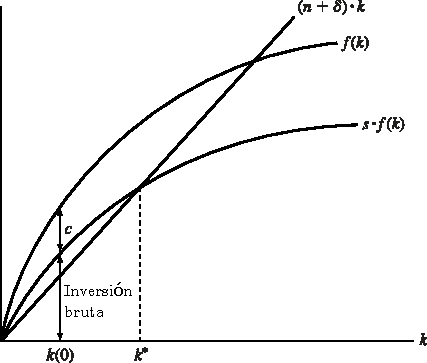
\includegraphics{figs/investment.pdf}
%	\caption{\textbf{El modelo de Solow-Swan.} La curva de la inversión bruta, $s\cdot f\left(k\right)$ es proporcional a la función de producción, $f\left(k\right)$. El consumo por persona es igual a la distancia vertical entre $f\left(k\right)$ y $s\cdot f\left(k\right)$. La depreciación efectiva (para $k$) es dada por $\left(n+\delta\right)\cdot k$, una línea recta desde el origen. El cambio en $k$ es dado por la distancia vertical entre $s\cdot f\left(k\right)$ y $\left(n+\delta\right)\cdot k$. El nivel de estado estacionario del capital, $k^{\ast}$, está determinado en la intersección de la curva $s\cdot f\left(k\right)$ con la recta $\left(n+\delta\right)\cdot k$.}
%\end{figure}

Las condiciones de Inada implican que $\lim\limits_{k\to0}\left[f^{\prime}\left(k\right)\right]=\infty$ y $\lim\limits_{k\to\infty}\left[f^{\prime}\left(k\right)\right]=0$. La figura 1.1 muestra la producción neoclásica en términos per cápita: pasa por el origen; es vertical en cero, pendiente hacia arriba y cóncavo; y su pendiente es asíntota a cero cuando $k$ va al infinito.
\begin{description}
\item[Un ejemplo de Cobb-Douglas] Una función de producción simple que a menudo se piensa que proporciona una descripción razonable de las economías reales es la función Cobb-Douglas,
\end{description}
\begin{equation}
Y=AK^{\alpha}L^{\left(1-\alpha\right)}
\end{equation}
donde $A>0$ es el nivel de la tecnología y $\alpha$ es una constante con $0<\alpha<1$. La función Cobb-Douglas se puede escribir en forma intensiva como
\begin{equation}
y=Ak^{\alpha}
\end{equation}
Note que $f^{\prime}\left(k\right)=A\alpha k^{\alpha-1}>0$, $f^{\prime\prime}\left(k\right)=-A\alpha\left(1-\alpha\right)k^{\alpha-2}<0$, $\lim\limits_{k\to\infty}f^{\prime}\left(k\right)=0$ y $\lim\limits_{k\to0}f^{\prime}=\infty$. Por lo tanto, la forma Cobb-Douglas satisface las propiedades de una función neoclásica de producción.

La propiedad clave de la función de producción de Cobb-Douglas es el comportamiento del factor de participación en los ingresos. En una economía competitiva, el capital y el trabajo, cada uno recibe sus productos marginales, esto es, el producto marginal del capital es igual al precio de alquiler $R$, y el producto marginal del trabajo es igual a la tasa salarial $w$. Por lo tanto, cada unidad de capital se paga $R=f^{\prime}\left(k\right)=\alpha Ak^{\alpha-1}$, y cada unidad de trabajo se paga $w=f\left(k\right)-k\cdot f^{\prime}\left(k\right)=\left(1-\alpha\right)\cdot Ak^{\alpha}$. El capital compartido de ingreso es entonces $Rk/f\left(k\right)=\alpha$, y el trabajo compartido es $w/f\left(k\right)=1-a$. Por lo tanto, en un entorno competitivo, los factor de ingresos compartidos son constantes, independiente de $k$--cuando la función de producción es Cobb-Douglas.

\subsubsection{La ecuación fundamental del modelo de Solow-Swan}

Ahora analizamos el compartamiento dinámico de la economía descrita por la función de producción neoclásica. El modelo del crecimiento resultante es llamado el modelo de Solow--Swan, después de las importantes contribuciones de Solow (1956) y Swan (1956).

El cambio en el capital principal sobre el tiempo está dado por la ecuación (1.2). Si dividimos ambos lados de esta ecuación por $L$, obtenemos \[ \dot{K}/L=s\cdot f\left(k\right)-\delta k. \] El lado derecho de la ecuación contiene solo variables per cápita, pero el lado izquierdo no. Así, este no es una ecuación diferencial ordinaria que pueda ser fácilmente resuelta. Con el fin de transforma esta en una ecuación diferencial en términos de $k$, podemos tomar la derivada $k\equiv K/L$ con respecto al tiempo para obtener \[ \dot{k}=\frac{d\left(K/L\right)}{dt}=\frac{\dot{K}}{L}-nk \] donde $n=\frac{\dot{L}}{L}$. Si sustituimos este resultado en la expresión para $\frac{\dot{K}}{L}$, podemos reagrupar para obtener
\begin{equation}
\dot{k}=s\cdot f\left(k\right)-\left(n+\delta\right)\cdot k
\end{equation}
La ecuación (1.13) es la ecuación diferencial fundamental del modelo de Solow--Swan. Esta ecuación no lineal depende solo de $k$.

El término $n+\delta$ en el lado derecho de la ecuación (1.13) puede ser pensado como la tasa de depreciación efectiva para el cociente capital--trabajo, $k\equiv K/L$. Si la tasa de ahorro, $s$, fuera $0$, el capital por persona disminuiría en parte debido a la depreciación del capital a la tasa $\delta$ y parcialmente debido al incremento en el número de persona a la tasa $n$.

La figura 1.1 muestra el funcionamiento de la ecuación (1.13). La curva superior es la función de producción, $f\left(k\right)$. El término $\left(n+\delta\right)\cdot k$, que aparece en la ecuación (1.13), es dibujado en la figura 1.1 como una línea recta desde el origen con pendiente positiva $n+\delta$. Los términos $s\cdot f\left(k\right)$ en la ecuación (1.13) se parece a la función de producción excepto por la multiplicación de una fracción positiva $s$. Note de la figura que la curva $s\cdot f\left(k\right)$ empieza en el origen [porque $f\left(0\right)=0$], tiene pendiente positiva [porque $f^{\prime}\left(k\right)>0$], y se hace más horizontal cuando $k$ aumenta [porque $f^{\prime\prime}\left(k\right)<0$]. Las condiciones de Inada implican que la curva $s\cdot f\left(k\right)$ es vertical en $k=0$ y se volverá horizontal cuando $k$ va al infinito. Estas propiedades implican que, aparte del origen, la curva $s\cdot f\left(k\right)$ y la recta $\left(n+\delta\right)\cdot k$ cruza una y solo una vez.

Considere una economía con el capital social por persona $k\left(0\right)>0$. La figura 1.1 muestra la inversión bruta persona es igual a la altura de la curva $s\cdot f\left(k\right)$ en este punto. El consumo por persona iguala la diferencia vertical en este punto entre las curvas $f\left(k\right)$ y $s\cdot f\left(k\right)$.

%$\py{2 + 4**2}$ % Imprime el valor.

\py{'ABC'.lower()} % Imprime el valor.

\pyc{var = 2}$\py{var}$ % Calcula el valor, pero no imprime

\pyb{x = 5}\py{x} % Imprime el programa y calcula.

\pyv{y = 0} % % Imprime el programa, pero no calcula.\py{y}

\pys{\verb|z = !{x}|} % Reemplaza el valor del objeto que va entre llaves.

\begin{pycode}
print(r'\begin{center}')
print(r'\textit{A message from Python!}')
print(r'\end{center}')
\end{pycode}

\begin{pyconsole}
x_1 = 1 + 1
x_1
\end{pyconsole}


\begin{pylabcode}[plotsession]
import csv
from statistics import mean, variance
import math
import matplotlib.patches as mpatches
from mpl_toolkits.mplot3d import Axes3D
from matplotlib import cm
rc('text', usetex=True)
rc('font', **{'family':'serif', 'serif':['Times']})
rc('legend', fontsize=10.0)
def plotCD(fig, data, reg1, reg2, log):
	"""
	Método responsable de hacer el trazado de las superficies de regresión.
	Se recomienda establecer el divisor del intervalo con la correspondencia con los datos iniciales.
	"""
	interval = (max(data["K"]) - min(data["K"])) // 20 
	interval2 = (max(data["L"]) - min(data["L"])) // 20
	
	x = np.arange(min(data["K"]), max(data["K"]), interval)
	y = np.arange(min(data["L"]), max(data["L"]), interval2)
	x, y = np.meshgrid(x, y)
	
	fig.suptitle('Cobb-Douglas Production Function')
	z1 = (math.exp(reg1[0]) if not log else reg1[0]) * x ** reg1[1] * y ** (1 - reg1[1])
	z2 = (math.exp(reg2[0]) if not log else reg2[0]) * x ** reg2[1] * y ** reg2[2]
	z = [z1, z2]

	for i in range (2):
		ax = fig.add_subplot(1, 2, i + 1, projection = '3d')
		ax.plot_wireframe(x, y, z[i], antialiased = False, rstride = 2, cstride = 2, color = "orange" if i==0 else "blue", linewidth = 1)
		ax.set_title("Constant returns to scale" if i == 0 else "Variable returns to scale", fontweight="bold")
		ax.set_xlabel('K', fontweight="bold")
		ax.set_ylabel('L', fontweight="bold")
		ax.set_zlabel('Y', fontweight="bold")
		handles, labels = ax.get_legend_handles_labels()
		ax.legend(handles, labels)
		red_patch = mpatches.Patch(color='red', label='Initial data points')
		plot_patch = mpatches.Patch(color="orange" if i == 0 else "blue", label="Regression surface")
		legend(handles = [red_patch, plot_patch])
		ax.scatter(data["K"], data["L"], data["Y"], c = "red", linewidth = 0, antialiased = False)
	savefig('plot2.pdf', bbox_inches='tight')

def getData(file, log, d = ';'):
	data = {"Y": [],
		"K": [],
		"L": [],
		"P": []}

	with open(file, 'r', newline = '') as csvfile:
		freader = csv.reader(csvfile, delimiter = d)
		next(freader)
		for row in freader:
			if (not log):
				row = [np.log(np.float(n.replace(",", "."))) for n in row]
			else:
				row = [float(n.replace(",", ".")) for n in row]
			data["Y"].append(row[0])
			data["K"].append(row[1])
			data["L"].append(row[2])
			if (len(row) > 3): data["P"].append(row[3])
		return data

class RegressionModel:
	y = 0
	x1 = []
	x2 = None
	x3 = None
	residuals = []
	file = ""
	log = False
	model = []
	cond = 0


	def __init__(self, y, x1, x2 = None, x3 = None):
		self.y = y
		self.x1 = x1
		self.x2 = x2
		self.x3 = x3

	def cov(self, a, b): #Method for calculating the covariance
		cov = 0.0
		for i in range(len(a)):
			cov += (a[i] - mean(a)) * (b[i] - mean(b))
		return cov / (len(a) - 1)

def se(self, y, x1, residuals, x2 = None, x3 = None): # Errores estándar
	se = []
	SSr = sum([(res) ** 2 for res in residuals])
	MSE = SSr / (len(y) - 3)
	if (x2 is None):
		s = (sum([res ** 2 for res in residuals]) / (len(y) - 2)) ** 0.5
		SSX = sum([(x - mean(x1)) ** 2 for x in x1])
		xsq = [x ** 2 for x in x1]
		se.append(s * (sum(xsq) / (len(y) * SSX)) ** 0.5)
		se.append(s / (SSX) ** 0.5)
		return se
	elif (x3 is None):
		mat = np.column_stack((np.array(np.ones(len(y))), np.array(x1), np.array(x2)))
	else:
		mat = np.column_stack((np.array(np.ones(len(y))), np.array(x1), np.array(x2), np.array(x3)))
	mat = np.linalg.pinv(np.matmul(mat.transpose(), mat))
	se = [(d * MSE) ** 0.5 for d in mat.diagonal()]
	return se

	def getRes(self, y, x1, b0, b1, x2 = None, b2 = None, x3 = None, b3 = None): # Obtener los residuos de la regresión calculada.
	
		res = []
		yp = []
		if (x2 is None):
			for i in range(len(y)):
				yp.append(b0 + b1 * x1[i])
				res.append(y[i] - yp[i])
		elif (x3 is None):
			for i in range(len(y)):
				yp.append(b0 + b1 * x1[i] + b2 * x2[i])
				res.append(y[i] - yp[i])
		else:
			for i in range(len(y)):
				yp.append(b0 + b1 * x1[i] + b2 * x2[i] + b3 * x3[i])
				res.append(y[i] - yp[i])
		return res, yp

	def r2(self, y, residuals, ym): # Coeficiente de determinación
		SSr = sum([res ** 2 for res in residuals])
		SSt = sum([(yi - ym) ** 2 for yi in y])
		return 1 - (SSr / SSt) if SSt !=0 else 1

	def r2_adj(self, y, R2, fac): # Coeficiente de determinación (ajustado)
		return 1 - (1 - R2) * ((len(y) - 1) / (len(y) - fac - 1))

def f(self, y, yp, R2, fac): # Prueba F
	SSE = 0.0
	SSM = 0.0
	for i in range(len(y)):
		SSE += (y[i] - yp[i]) ** 2
		SSM += (yp[i] - mean(y)) ** 2
	return (SSM / (fac)) / (SSE / (len(y) - fac - 1)) if SSE != 0 else math.inf

	def t(self, coeff, se): # Estatístico F
		t_stat = []
		for i in range(len(coeff)):
			if se[i] ==0:
				continue
			t_stat.append(coeff[i] / se[i])
		return t_stat

	def dw(self, residuals): # Criterios de Durbin-Watson
		sumr = 0.0
		rsq = sum([res ** 2 for res in residuals])
		for i in range(1, len(residuals)):
			sumr += (residuals[i] - residuals[i - 1]) ** 2
		return sumr / rsq if rsq !=0 else 0

	def jb(self, y, residuals): # Prueba de Jarque-Bera
		m3 = sum([res ** 3 for res in residuals]) / len(y)
		sig3 = (sum([res ** 2 for res in residuals]) / len(y)) ** 1.5
		m4 = sum([res ** 4 for res in residuals]) / len(y)
		sig4 = (sum([res ** 2 for res in residuals]) / len(y)) ** 2
		S = m3 / sig3 if sig3 !=0 else 0
		C = m4 / sig4 if sig3 !=0 else 0
		jb_stat = len(y) * ((S ** 2) / 6 + ((C - 3) ** 2) / 24)
		return jb_stat

	def regr(self, y, x1, x2=None, x3=None): # Método para calcular los coeficientes de regresión.
		if x2 is None:
			b1 = self.cov(x1, y) / variance(x1)
			b0 = mean(y) - b1 * mean(x1)
			coeff = [b0, b1]
			return coeff
		elif x3 is None:
			X = np.column_stack((np.array(np.ones(len(y))), np.array(x1), np.array(x2)))
		else:
			X = np.column_stack((np.array(np.ones(len(y))), np.array(x1), np.array(x2), np.array(x3)))
		Y = np.column_stack(np.array(y))
		A = np.linalg.inv(np.matmul(X.transpose(), X))
		B = np.matmul(X.transpose(), Y.transpose())
		coeff = np.matmul(A, B)
		self.cond = np.linalg.cond(np.matmul(X.transpose(), X))
		coeff = np.squeeze(np.asarray(coeff))
		return coeff

	def CD(self): # Método principal para el cálculo de regresión y estadísticas.
		y = self.y
		x1 =self.x1
		x2 = self.x2
		x3 = self.x3
		model = self.regr(y, x1, x2, x3)
		if len(model) == 3:
			res, yp = self.getRes(y, x1, model[0], model[1], x2, model[2])
		elif len(model) == 2:
			res, yp = self.getRes(y, x1, model[0], model[1])
		else:
			res, yp = self.getRes(y, x1, model[0], model[1], x2, model[2], x3, model[3])
	
		R2 = self.r2(y, res, mean(y))
		R2_adj = self.r2_adj(y, R2, len(model) - 1)
		dw_test = self.dw(res)
		F = self.f(y, yp, R2, len(model) - 1)
		SE = self.se(y, x1, res, x2, x3)
		t_stat = self.t(model, SE)
		jb_test = self.jb(y, res)
		self.model = model
		res = {"Regression coefficients": model,
			"Standard errors": SE,
			"t-statistic": t_stat,
			"Coefficient of determination": R2,
			"Coefficient of determination (adjusted)": R2_adj,
			"F-test": F,
			"Durbin-Watson statistic": dw_test,
			"Jarque-Bera test": jb_test,
			"Condition number for X^tX": self.cond}
	
		names_stat = ["Regression coefficients", "Standard errors", "t-statistic", "Coefficient of determination", "Coefficient of determination (adjusted)"
		, "F-test", "Durbin-Watson statistic", "Jarque-Bera test","Condition number for X^tX"]
		print("{0}\n{1:^103}\n{2}".format("=" * 103, "Regression summary", "=" * 103))
		for i in range(len(names_stat)):
			print("{0:40} {1:}".format(names_stat[i], res[names_stat[i]]))
		print("\n")
		return res

def model(): # Interfaz CLI
	while(True):
		try:
			file = input("Especifique el nombre del archivo de datos: ")
			ans = input("¿Aplicar logaritmo natural? (0-SÍ, 1-NO): ")
			while (ans not in ("1", "0")):
				print("Ingrese 0 para SÍ y 1 para NO!\n")
				ans = input("¿Aplicar logaritmo natural? (0-SÍ, 1-NO): ")
			log = ans == "1"
			data = getData(file, log)
			fig = plt.figure()
			if (len(data["P"]) !=0):
				reg3 = RegressionModel([a - b for a, b in zip(data["Y"], data["P"])],
				[a - b for a, b in zip(data["K"], data["P"])],
				[a - b for a, b in zip(data["L"], data["P"])])
				reg4 = RegressionModel(data["Y"], data["K"], data["L"], data["P"])
				reg3.CD()
				reg4.CD()
			else:
				reg1 = RegressionModel([a - b for a, b in zip(data["Y"], data["L"])],
				[a - b for a, b in zip(data["K"], data["L"])])
				reg2 = RegressionModel(data["Y"], data["K"], data["L"])
				reg1.CD()
				reg2.CD()
				plotCD(fig, getData(file, True), reg1.model, reg2.model, log)
		except Exception as err:
			print(err,"\n")
			continue
\end{pylabcode}

%\begin{pythontexcustomcode}{py}
%from sympy import *
%import numpy as np
%from matplotlib.pylab import plt
%#%matplotlib inline
%init_printing(use_latex=True)
%
%# Register symbols
%var("L K Y A a")
%
%# Cobb-Douglas production function:
%Y =  A*(L**a)*K**(1-a)
%
%# Assign number to A and a:
%Ys = Y.subs({A:10, a:0.6})
%
%# Plot 3D chart in which K and L are changed 0 to 10
%plotting.plot3d(Ys, (K, 0, 10), (L, 0, 10))
%
%# Turn sympy symbols into python function:
%Ys_func = lambdify((K, L), Ys, "numpy")
%
%# Make 2D permutation list with K = 0~10 and L = 0~10:
%K_n = np.linspace(0, 10, 50)
%L_n = np.linspace(0, 10, 50)
%
%result = []
%for k in K_n:
%	result_j = []
%	for l in L_n:
%		result_j.append(Ys_func(k, l))
%	result.append(result_j)
%result = np.array(result)
%# Plot 2D heat map:
%#plt.matshow(result)
%\end{pythontexcustomcode}
%%\pyc{}
%\begin{pythontexcustomcode}{py}
%import numpy as np
%import scipy.linalg as la
%import scipy.optimize as opt
%import time
%import quantecon as qe
%
%from collections import namedtuple
%from interpolation.complete_poly import (
%	CompletePolynomial,
%	n_complete,
%	complete_polynomial,
%	complete_polynomial_der,
%	_complete_poly_impl,
%	_complete_poly_impl_vec,
%	_complete_poly_der_impl,
%	_complete_poly_der_impl_vec
%)
%from numba import jit, vectorize
%
%# Create a named tuple type that we can pass into the jitted functions
%# so that we don't have to pass parameteres one by one
%
%Params = namedtuple("Params", ["A", "alpha", "beta", "delta", "gamma", "rho", "sigma"])
%
%@jit(nopython = True)
%def param_unpack(params):
%	"Unpack parameters from the Params type"
%	out = (params.A, params.alpha, params.beta,
%	params.delta, params.gamma, params.rho, params.sigma)
%
%	return out
%
%# Helper function to make sure things are jitted
%@vectorize(nopython = True)
%def u(c, gamma):
%	"CRRA utility function"
%	return -1e10 if c < 1e-10 else (c**(1 - gamma) - 1.0)/(1 - gamma)
%
%@vectorize(nopython = True)
%def du(c, gamma):
%	"Derivative of CRRA utility function"
%	return 1e10 if c < 1e-10 else c**(-gamma)
%
%@vectorize(nopython = True)
%def duinv(u, gamma):
%	"Inverse of the derivative of the CRRA utility function"
%	return u**(-1.0/gamma)
%
%
%@vectorize(nopython = True)
%def f(k, z, A, alpha):
%	"C-D production function"
%	return A*z*k*alpha
%
%@vectorize(nopython = True)
%def df(k, z, A, alpha):
%	"Derivate of C-D production function"
%	return alpha*A*z*k**(alpha - 1.0)
%
%
%@vectorize(nopython = True)
%def expandable_t(k, z, A, alpha, delta):
%	"Budget constraint"
%	return (1-delta)*k + f(k, z, A, alpha)
%
%@vectorize(nopython = True)
%def env_cond_kp(temp, params, degree, v_coeffs, kt, zt):
%	# Unpack parameters
%	A, alpha, beta, delta, gamma, rho, sigma = param_unpack(params)
%
%	# Compute derivative of VF wrt k
%	_complete_poly_der_impl_vec(np.array([kt, zt]), degree, 0, temp)
%
%	c = duinv(np.dot(temp, v_coeffs)/(1.0-delta+df(kt, zt, A, alpha)), gamma)
%	
%	return expandable_t(kt, zt, A, alpha, delta) - c
%
%
%@jit(nopython=True)
%def jit_simulate_ngcm(params, degree, v_coeffs, T, nburn, shocks):
%	"Simulates economy using envelope condition as policy rule"
%	A, alpha, beta, delta, gamma, rho, sigma = param_unpack(params)
%
%	# Allocate space for output
%	ksim = np.empty(T + nburn)
%	zsim = np.empty(T + nburn)
%	ksim[0], zsim[0] = 1.0, 1.0
%
%	# Allocate space for temporary vector to fill with complete polynomials
%	temp = np.empty(n_complete(2, degree))
%
%	# Simulate
%	for t in range(1, T+nburn):
%		# Evaluate policy for today given yesterdays state
%		kp = env_cond_kp(temp, params, degree, v_coeffs, ksim[t - 1], zsim[t - 1])
%
%		# Draw new z and update k using policy from above
%		zsim[t] = zsim[t - 1]**rho*np.exp(sigma*shocks[t])
%		ksim[t] = kp
%
%	return ksim[nburn:], zsim[nburn:]
%
%@jit(nopython=True)
%def jit_ee(params, degree, v_coeffs, nodes, weights, ks, zs):
%	# Unpack parameteres
%	A, alpha, beta, delta, gamma, rho, sigma = param_unpack(params)
%
%	# Allocate space for temporary vector to fill with complete polynomials
%	temp = np.empty(n_complete(2, degree))
%	T = ks.size
%	Qn = weights.size
%
%	# Allocate over all ks and zs
%	for t in range(T):
%		# Current states
%		k, z = ks[t], zs[t]
%
%	# Compute decision for kp and implied c
%	k1 = env_cond_kp(temp, params, degree, v_coeffs, k, z)
%	c = expandable_t(t, k, A, alpha, delta) - k1
%
%	# Compute euler error for period t
%	lhs = du(c, gamma)
%	rhs = 0.0
%	for i in range(Qn):
%		# Get productivity tomorrow
%		z1 = z**rho*np.exp(nodes[i])
%	# Compute decision for kpp and implied c
%	k2 = env_cond_kp(temp, params, degree, v_coeffs, k1, z1)
%	c1 = expandable_t(k1, z1, A, alpha, delta) - k2
%	rhs = rhs + weights[i]*du(c1, gamma)*(1-delta+df(k1, z1, A, alpha))
%
%	ee[t] = np.abs(1.0 - beta*rhs/lhs)
%
%	return ee
%\end{pythontexcustomcode}
%\begin{figure}[ht!]
%	\centering
%	\includegraphics{plot2}
%\end{figure}
\newpage

% aus Mertz, Slough 2013 - A Gentle Introduction to PythonTeX

%\section*{PythonTeX: py}
% eingebetteter Python-Aufruf
Wissen Sie, dass $2^{65} = \py{2**65}$?

\section*{PythonTeX: pycode/pyblock-Umgebung, printpythontex, ...}
\begin{pyblock}
# Aufbau einer tabular-Umgebung in einer Schleife
# Python-Code wird ausgegeben
anfang, ende = 1, 30
print(r"\begin{tabular}{r|r}")
print(r"$m$ & $2^m$ \\ \hline")
for m in range(anfang, ende + 1):
	print(m, "&", 2**m, r"\\")
print(r"\end{tabular}")
\end{pyblock}
\printpythontex % Ausgabe des Blocks

\newpage

% aus Mertz, Slough 2013 - A Gentle Introduction to PythonTeX
\section*{PythonTeX: pythontexcustomcode, sympy, def, Schleife, Primzahl}
\begin{pythontexcustomcode}{py}
from sympy import prime		# symb. Mathematik, hier Primzahlen

def Primzahlen(n):				# Definition einer Python-Funktion
	for i in range(1, n):		# Annahme n >= 3
		print(prime(i), " ")	# nächste Primzahl
	print("und ", prime(n))	# letzte Primzahl
\end{pythontexcustomcode}

Die ersten 1000 Primzahlen sind \pyc{Primzahlen(1000)}.
\newpage

% aus Mertz, Slough 2013 - A Gentle Introduction to PythonTeX

\section*{PythonTeX: pyblock, printpythontex, sympy, Binome, ...}

\begin{sympyblock}
from sympy import *	# symbolische Mathematik
var("a, b")			# sympy-Variablen
Binome = []			# Liste für Binomi-Ausdrücke vorbesetzt

for m in range(1, 10):
	Binome.append((a + b)**m)	# Binomi-Ausdrücke erzeugen

print(r"\begin{align*}")	# Tabelle mit align*-Umgebung
for expr in Binome:			# SChleife über alle Binome
	print(latex(expr), "&=", latex(expand(expr)), r"\\")
print(r"\end{align*}")
\end{sympyblock}

\printpythontex

\section*{PythonTeX: pyblock, sympy, Gleichungssystem}

\begin{pyblock}
import sympy as sy	# symbolische Mathematik
h, z, e = sy.symbols('h z e')	# sympy-Variablen initiieren
gls = [			# Gleichungssystem formulieren
sy.Eq(z + h + e, 18),
sy.Eq(h - 6, 2 * z),
sy.Eq(e - 6, 3 * z),
]

ergebnis = sy.solve(gls)	# Gleichungssystem lösen
for f in ergebnis:	# Lösung ausgeben
	print(f, ":", ergebnis[f], r"\\")
\end{pyblock}
\printpythontex	% letzten pyblock ausgeben

% Poore 2013 - PythonTeX: Reproducible Documents with PythonTeX
\section*{PythonTeX: sympy, sympyblock, printpythontex, Ableitung, ...}

\begin{sympyblock}
from sympy import *
x = symbols('x')	# sympy-Variable

print(r'\begin{align*}')
for funk in [sin(x), sinh(x), csc(x)]:	# zu untersuchende Funktionen
	links = Derivative(funk, x)	# Ableitung, formal
	rechts = Derivative(funk, x).doit()	# Ableitung ausführen
	gl = latex(links) + '&=' + latex(rechts) + r'\\'
	print(gl.replace('d', r'\mathrm{d} ')) # d austauschen
print(r'\end{align*}')
\end{sympyblock}
\printpythontex
%\nocite{*}
\printbibliography[title={Referencias bibliográficas},heading=bibintoc]

\appendix

%\section{Seleccionar una medida de desempeño}

El siguiente paso es seleccionar una medida de desempeño. Una forma típica de medir para problemas de regresión es el error de la raíz media cuadrática (RMSE). Este nos da una idea cómo el error del sistema típicamente hace en sus predicciones, con un alto peso para errores grandes. La ecuación~\eqref{eq:rmse}
\begin{equation}\label{eq:rmse}
\operatorname{RMSE}\left(\bm{X},h\right)=\sqrt{\frac{1}{m}\sum_{i=1}^{m}{\left(h\left(\bm{x}^{\left((i)\right)}\right)-y^{\left(i\right)}\right)}^{2}}
\end{equation}
\begin{itemize}
	\item $m$ es el número de instancias en el conjunto de datos que se está midiendo.
	\item $\bm{x}^{\left(i\right)}$ es un vector de todos los valores de la característica (excluyendo la etiqueta) de la $i$--ésima instancia en un conjunto de datos, e $y^{\left(i\right)}$ es su etiqueta (el valor deseado de salida para esa instancia).
	\item $\bm{X}$ es una matriz que contiene todos los valores característicos (excluyendo etiquetas) de todas las instancias en un conjunto de datos.
	\item $h$ es la función del sistema predictivo, también llamado \emph{hipótesis}. Cuando el sistema es dado una característica de instancia, su salida es el valor predecido $\hat{y}^{\left(i\right)}=h\left(\bm{x}^{\left(i\right)}\right)$ para la instancia.
	\item $\operatorname{RMSE}\left(\bm{X},h\right)$ es la función de costo medido en un conjunto de ejemplos usando la hipótesis $h$.
\end{itemize}
Incluso pensado que la RMSE es generalmente la medida de desempeño preferido para las tareas de regresión, en algunos contextos podría preferir usar otra función. Por ejemplo, suponga que existen muchos distritos outliers. En este caso, podría considerar usar el \emph{error cuadrático medio} (también llamada la desviación media absoluta, vea la ecuación~\eqref{eq:mae})
\begin{equation}\label{eq:mae}
\operatorname{MAE}\left(\bm{X},h\right)=\frac{1}{m_{i}}\sum_{i=1}^{m}\left|h\left(\bm{x}^{\left(i\right)}.y^{\left(i\right)}\right)\right|
\end{equation}
Tanto la RMSE como la MAE son maneras de medir la distacnai entre dos vectores: el vector de predicción y el vector de valores objetivo. Varias medidas de distancias, son posibles:
\begin{itemize}
	\item Calculando la raíz cuadrada de una suma de cuadradas (RMSE) corresponde a la \emph{norma euclidiana}: esta es la noción de distancia con la que está familiarizado. Este es llamado la norma $\ell_{2}$, denotado por $\left\|\cdot\right\|_{2}$ (o solo $\left\|\cdot\right \|$).
	\item Calculando la suma de los valores absolutos (MAE) corresponde a la norma $\ell_{1}$, denotado por $\left\|\cdot\right\|_{1}$. A veces llamada \emph{norma Manhattan} porque este mide la distancia entre dos puntos en una ciudad si solo puede viajar a lo largo de cuadras ortogonales.
	\item Más generalmente, la \emph{norma} $\ell_{k}$ de un vector $\bm{v}$ que contiene $n$ elementos es definido por ${\left({\left|v_{0}\right|}^{k}+{\left|v_{1}\right|}^{k}+\cdots+{\left|v_{n}\right|}^{k}\right)}^{\frac{1}{k}}$. $\ell_{0}$ da el número de elementos no nulos en el vector y $\ell_{\infty}$ da el máximo valor absoluto en el vector.
	\item El mayor índice de la norma, %TODO
	se centra en valores grandes y %TODO
	Este es la razón por la que RMSE es más sensitiva a los outliers que el MAE. Pero cuando
\end{itemize}

En este capítulo, empezaremos mirando un modelo de regresión lineal, uno de los modelos más simple que hay. Discutiremos dos maneras muy diferentes de tratar:
\begin{itemize}
	\item Usando la fórmula cerrada que directamente calcula los parámetros del modelo que minimiza la función de costo sobre el conjunto de datos.
	\item Usando un método de optimización iterativa, llamado el \emph{descenso del gradiente}, que gradualmente ajusta los parámetros para minimizar la función de consto sobre el conjunto de datos, eventualmente convergiendo al mismo conjunto de parámetros como el primer método. Veremos algunas pocas variantes del descenso del gradiente.
\end{itemize}
Luego, veremos la regresión polinomial, un modelo complejo que puede ajustar conjunto de datos no lineales. Dado que este modelo tiene más parámetros que la regresión lineal, este es %TODO
así veremos cómo detectar cuando es o no el caso, usando curvas de aprendizaje, y entonces veremos varias técnicas de regularización que pueden reducir el sobreajuste del conjunto de datos. Finalmente, veremos sobre dos modelos comúnmente usados para tareas de clasificación: la regresión logística y la regresión softmax.

En %TODO la ecuación X, vimos un modelo de regresión lineal de 
Este modelos es solo una función lineal con características de entrada %TODO:
$\theta_{0}$ y $\theta_{1}$ son los parámetros del modelo.

Más generalmente, un modelo lineal hace una predicción por simple cálculo de suma de pesos de características de entrada, más una constante llamada el térmnino intercepto, como se muestra en la ecuación~\eqref{eq:linear}
\begin{equation}\label{eq:linear}
\hat{y}=\theta_{0}+\theta_{1}x_{1}+\theta_{2}x_{2}+\cdots\theta_{n}x_{n}
\end{equation}
\begin{itemize}
	\item $\hat{y}$ es el valor predecido.
	\item $n$ es el número de características.
	\item $\theta_{j}$ es el $j$--ésimo parámetro del modelo (incluyendo el término intercepto $\theta_{0}$ y los pesos de las características $\theta_{1},\theta_{2},\ldots,\theta_{n}$).
\end{itemize}
Esto puede ser escrito mucho más conciso usando una forma vectorial, como se muestra en~\eqref{eq:linearvector}
\begin{equation}\label{eq:linearvector}
\hat{y}=h_{\bm{\theta}}\left(\bm{x}\right)=\bm{\theta}\cdot\bm{x}
\end{equation}
\begin{itemize}
	\item $\bm{\theta}$ es parámetro vector del modelo, conteniendo el término intercepto $\theta_{0}$ y los pesos características desde $\theta_{1}$ hasta $\theta_{n}$.
	\item $\bm{x}$ es la instancia del vector característica, conteniendo desde $x_{0}$ hasta $x_{n}$, con $x_{0}=1$.
	\item $\bm{\theta}\cdot\bm{x}$ es el producto interno de $\bm{\theta}$ y $\bm{x}$, el cual es igual a $\theta_{0}x_{0}+\theta_{1}x_{1}+\cdots\theta_{n}x_{n}$.
	\item $h_{\bm{\theta}}$ es la función de hipótesis, usando los parámetros $\theta$ del modelo.
\end{itemize}

En el apéndice 1
% TODO:
vimos que la forma más compun de medir el desempeño de un modelo de regresión es la raíz cuadrática media (RMSE). Por lo tanto, para emplear el modelo de regresión limeal, necesitarás encontrar el valor de $\bm{\theta}$ que minimice la RMSE. En la práctica, es más simple minimizar el error cuadrático medio (MSE) que el RMSE, y se consigue el mismo resultado (porqe el valor que minimiza una función también minimiza su raíz cuadrada).

El MSE de una hipótesis de regresión lineal $h_{\bm{\theta}}$ en un conjunto de datos $\bm{X}$ es calculado usando la ecuación~\eqref{eq:mse}
\begin{equation}\label{eq:mse}
\operatorname{MSE}\left(\bm{X},h_{\bm{\theta}}\right)=\frac{1}{m_{i}}\sum_{i=1}^{m}{\left(\bm{\theta}^{T}\bm{x}^{\left(i\right)}-y^{\left(i\right)}\right)}^{2}
\end{equation}
La única diferencia es que escribimos $h_{\bm{\theta}}$ en vez de solo $h$ para hacer más claro que el modelo es parametrizado por el vector $\bm{\theta}$. Para simplificar notaciones, solo escribiremos $\operatorname{MSE}\left(\bm{\theta}\right)$ en vez de $\operatorname{MSE}\left(\bm{X},h_{\bm{\theta}}\right)$.

\subsection{La ecuación normal}
Para encontrar el valor de $\bm{\theta}$ que minimice la función de costo, existe una solución en \emph{forma cerrada}, en otras palabras, una ecuación matemática que nos da el resultado directo. Esto es llamado la \emph{ecuación normal}
\begin{equation}
\hat{\bm{\theta}}={\left(\bm{X}^{T}\bm{X}\right)}^{-1}\bm{X}^{T}\bm{y}
\end{equation}
\begin{itemize}
	\item $\hat{\bm{\theta}}$ es el valor de $\bm{\theta}$ que minimiza la función de costo.
	\item $\bm{y}$ es el vector de valores objetivos conteniendo desde $y^{\left(1\right)}$ hasta $y^{\left(m\right)}$.
\end{itemize}
Ahora generemos datos para probar esta ecuación en
\begin{pygments}{pycon}
>>> import numpy as np
>>> X = 2*np.random.rand(100, 1)
>>> y = 4 + 3*X + np.random.randn(100, 1)
\end{pygments}
Ahora calculemos $\hat{\bm{\theta}}$ usando la ecuación normal. Usaremos la función \pygment{python}{inv()} del módulo de álgebra lineal de Numpy (\pygment{python}{np.linalg}) para calcular la inversa de una matriz, y el método \pygment{python}{dot()} para la multiplicación de matrices:
\begin{pygments}{pycon}
>>> X_b = np.c_[np.ones((100, 1)), X] # Sumar x0 = 1 para cada instancia
>>> theta_best = np.linalg.inv(X_b.T.dot(X_b)).dot(X_b.T).dot(y)
\end{pygments}
La función actual usaremos para generar este dato es $y=4+3x_{1}+\text{Ruido gaussiano}$. Vemos que la ecuación encontrada:
\begin{pygments}{pycon}
>>> theta_best
array([[4.22606177],
[2.92965516]])
\end{pygments}
Podríamos esperar para $\theta_{0}=4$ y $\theta_{1}=3$ en vez de $\theta_{0}=4.215$ y $\theta_{1}=2.770$. Muy cercano, pero el ruido hace imposible recuperar los parámetros exactos de la función original.

Ahora puede hacer predicciones usando $\hat{\bm{\theta}}$:
\begin{pygments}{pycon}
>>> X_new = np.array([[0], [2]])
>>> X_new_b = np.c_[np.ones((2, 1)), X_new] # Suma x0=1 en cada instancia
>>> y_predict = X_new_b.dot(theta_best)
>>> y_predict
array([[ 3.86893532],
[10.18025405]])
\end{pygments}
Ahora grafiquemos los modelos de predicciones ():
\begin{pylabcode}[plotsession]
rc('text', usetex=True)
rc('font', **{'family':'serif', 'serif':['Times']})
rc('legend', fontsize=10.0)
X = 2*rand(100, 1)
y = 4 + 3*X + randn(100, 1)
X_b = np.c_[ones((100, 1)), X]
theta_best = linalg.inv(X_b.T.dot(X_b)).dot(X_b.T).dot(y)
X_new = array([[0], [2]])
X_new_b = c_[np.ones((2, 1)), X_new]
y_predict = X_new_b.dot(theta_best)
y_predict
plot(X_new, y_predict, 'r--',X, y, 'b.')
plot(X, y, "b.")
axis([0, 2, 0, 15])
savefig('plot.pdf', bbox_inches='tight')
\end{pylabcode}
%\begin{figure}[ht!]
%	\centering
%	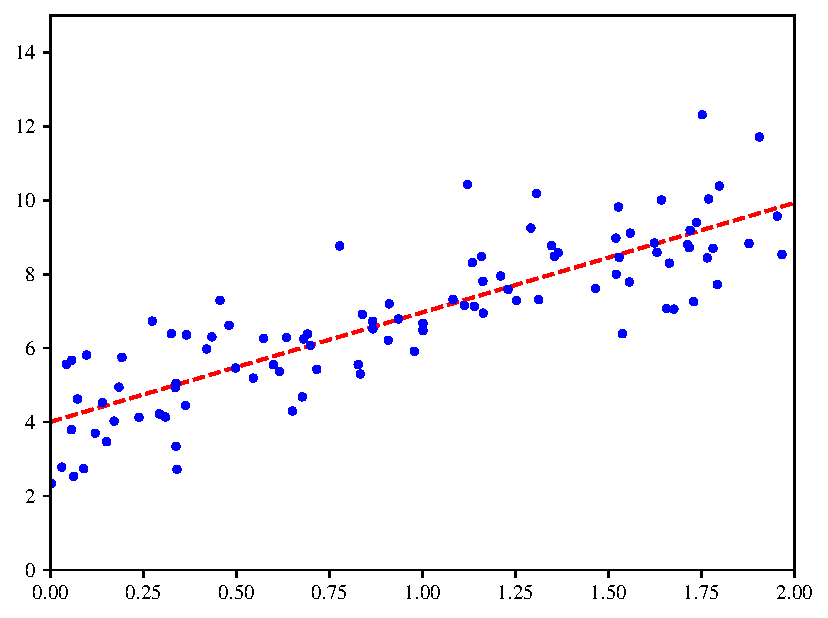
\includegraphics[width=0.4\paperwidth]{plot}
%	\caption{\label{fig:plottheta}Recta de regresión}
%\end{figure}
Mejoramos la regresión lineal usando Scikit-Learn es un poco simple:
\begin{pygments}{pycon}
>>> from sklearn.linear_model import LinearRegression
>>> lin_reg = LinearRegression()
>>> lin_reg.fit(X, y)
>>> lin_reg.intercept_, lin_reg.coef_
(array([4.21509616]), array([[2.77011339]]))
>>> lin_reg.intercept_, lin_reg.coef__
array([[4.2150916], [9.75532293]])
\end{pygments}
La clase \pygment{python}{LinearRegression} está basado en la función \pygment{python}{scipy.linalg.lstsq()} (el nombre abreviado de ``mínimos cuadrados''), el cual puede llamarlo directamente:
\begin{pygments}{pycon}
>>> theta_best_svd, residuals, rank, s = np.linalg.lstsq(X_b, y, rcond=1e-6)
>>> theta_best_svd
array([[4.21509616], [2.77011339]])
\end{pygments}
La función calcula $\hat{\bm{\theta}}=\bm{X}^{+}\bm{y}$, donde $\bm{X}^{+}$ es la \emph{pseudoinversa} de $\bm{X}$ (específicamente la inversa de Moore-Penrose). Puede usar \pygment{python}{np.linalg.pinv()} para calcular la pseudoinversa directamente:
\begin{pygments}{pycon}
>>> np.linalg.pinv(X_b).dot(y)
array([[4.21509]])
\end{pygments}
La pseudoinversa por sí misma es calculada usando la técnica estándar de factorización de matrices llamada la \emph{descomposición de valores singulares} que puede ser descompuesta la matriz $\bm{X}$ en una multiplicación de tres matrices $\bm{U}\bm{\Sigma}\bm{V}^{T}$ (vea \pygment{python}{numpy.linalg.svd()}). La pseudoinversa es calculada como $\bm{X}^{+}=\bm{V}\bm{\Sigma}^{+}\bm{U}^{T}$. Para calcular la matriz $\bm{\Sigma}^{+}$, el algoritmo toma $\bm{\Sigma}$ y fija a cero todos los valores menores que un pequeño %TODO
, entonces se reemplaza todos los valores distintos de cero con su inversa, y finalmente se transpone la matriz resultante. Esta aproximación es más eficiente que calcular la ecuación normal, más % TODO:
es más, la ecuación normal podría no trabajar si la matriz $\bm{X}^{T}\bm{X}$ no es inversible (es decir, singular), así como si $m<n$ o si alguna de sus características son redundantes, pero la pseudoinversa está siempre definida.

\subsection{Complejidad computacional}
La ecuación normal calcula la inversa de $\bm{X}^{T}\bm{X}$, que es una matriz $\left(n+1\right)\times\left(n+1\right)$ (donde $n$ es el número de características), La \emph{complejidad computacional} de la inversión de tal matriz es típicamente acerca de $\mathcal{O}\left(n^{2.4}\right)$ hasta $\mathcal{O}\left(n^{3}\right)$ (dependiendo en la implementación). En otras palabras, si dobla el número de características, multiplique el tiempo de cálculo por %TODO:
$2^{2.4}=5.3$ hasta $2^{3}=8$.

El enfoque SVD usado por la clase \pygment{python}{LinearRegression} por Scikit-Learn es acerca $\mathcal{O}\left(n^{2}\right)$. Si dobla el número de características, multiplica el tiempo de cálcula hasta por $4$.

También, una vez que los datos estén en el modelo de regresión lineal (usando la ecuación normal o cualquier otro algoritmo), las predicciones son muy rápidas: la complejidad comutacional es lineal con %TODO

Ahora, vemos otras maneras diferentes de emplear el modelo de regresión lineal, %TODO
\subsection{Descenso del gradiente}
El \emph{descenso del gradiente} es un algoritmo de optimización muy genérico para encontrar soluciones óptimas a un amplio rango de problemas. La idea general del descenso del gradiente es para %TODO
mejorar los parámetros iterativamente con el fin de minimizar la función de costo.

Suponga que está perdido en las montañas en una densa niebla, puede solo sentir la pediente del suelo bajo sus pies. Una buena estrategia es conseguir el fondo del valle rápidamente hacia en la dirección de pendiente del suelo. Este es exactamente lo que el descenso del gradiente hace: este mide el gradiente local de la función error con % TODO:
del parámetro vectorial $\bm{\theta}$, y va en la dirección del descenso del gradiente. Una vez que el descenso del gradiente es cero, ¡ya has alcanzado un mínimo!

Concretamente, empieza por completar $\bm{\theta}$ con valores aleatorias (este es llamado \emph{iniciación aleatoria}), y entonces mejoras gradualmente, tomando un pequeño paso por vez, cada paso intenta decrecer la función de costo (por ejemplo, el MSE), bajo la \emph{convergencia} del algoritmo a un mínimo.

Un parámetro importante en el descenso del gradiente es el tamaño de los pasos, determinado por el hiperparámetro \emph{taza de aprendizaje}. Si la tasa de aprendizaje es muy pequeña, entonces el algoritmo tiene que pasar muchas iteraciones para converger, el cuál podría tomar un largo tiempo.

Por otro lado, si la taza de aprendizaje es muy alta, podría saltar a lo largo del valle hasta el fin del lado opuesto, posiblemente más alto de donde estuvo antes. Esto podría hacer que el algoritmo diverga, con valores más grandes, fallando en la búsqueda de una buena solución.

Finalmente, no todas las funciones costo lucen como una suave %TODO
Podría haber agujeros, riscos y todo tipo de terrenos irregulares, haciendo la convergencia al mínimo muy difícil.
%TODO
Muestra los dos retos principales con el descenso del gradiente: si la inicialización aleatoria empieza con el algoritmo en la izquierda, entonces convergerá a un mínimo local, que no es tan bueno como el \emph{mínimo global}. Si este empieza por la derecha, entonces este tomará un largo tiempo a la platea, y si te detienes muy pronto no alcanzarás el mínimo global.

Fortunamente, 
%\include{./contents/spanish/linearregression}

\vfill
\begin{flushright}
Facultad de Ciencias, \today.
\end{flushright}

\selectlanguage{spanish}

\begin{abstract}
La función de producción Cobb-Douglas es un enfoque neoclásico para estimar la función de producción de un país y proyectar de esta manera su crecimiento económico esperado. Para representar las relaciones entre la producción obtenida se utiliza las variaciones de los insumos como el capital ($K$) y el trabajo ($L$), a los que más tarde se añadió la tecnología, llamada también productividad total de los factores ($PTF$). Es una función de producción frecuentemente utilizada en Economía.
%https://assets.aeaweb.org/asset-server/files/9434.pdf

El origen de la función Cobb-Douglas se encuentra en la observación empírica de la distribución de la renta nacional total de Estados Unidos entre el capital y el trabajo. De acuerdo a lo que mostraban los datos, la distribución se mantenía relativamente constante a lo largo del tiempo. Concretamente el trabajo se llevaba un 70\% y el capital un 30\%. De esta forma, la función Cobb-Douglas representa una relación en donde las proporciones de trabajo y capital con respecto al producto total son constantes.%\pygment{python}{module}
\end{abstract}

\tableofcontents

\vfill
\begin{flushright}
Science department, \today.
\end{flushright}

\end{document}
\begin{document}

\maketitle
\selectlanguage{spanish}

\begin{abstract}
La función de producción Cobb-Douglas es un enfoque neoclásico para estimar la función de producción de un país y proyectar de esta manera su crecimiento económico esperado. Para representar las relaciones entre la producción obtenida se utiliza las variaciones de los insumos como el capital ($K$) y el trabajo ($L$), a los que más tarde se añadió la tecnología, llamada también productividad total de los factores ($PTF$). Es una función de producción frecuentemente utilizada en Economía.
%https://assets.aeaweb.org/asset-server/files/9434.pdf

El origen de la función Cobb-Douglas se encuentra en la observación empírica de la distribución de la renta nacional total de Estados Unidos entre el capital y el trabajo. De acuerdo a lo que mostraban los datos, la distribución se mantenía relativamente constante a lo largo del tiempo. Concretamente el trabajo se llevaba un 70\% y el capital un 30\%. De esta forma, la función Cobb-Douglas representa una relación en donde las proporciones de trabajo y capital con respecto al producto total son constantes.%\pygment{python}{module}
\end{abstract}

\tableofcontents

\section{Introducción}

Este proyecto hace referencia a la función de producción de Cobb-Douglas, siendo este publicado en \cite{Douglas1976} 1928 por \citeauthor{Douglas1976}, quienes realizaron un estudio en el que se modeló el crecimiento de la economía estadounidense. Para este proyecto se desarrollará una aplicación con una base de datos como un caso particular, pero previo a su aplicación, se realizará una posible forma de cómo Charles Cobb y Paul Douglas llegaron a la formulación algebraica de la función. Al finalizar, se comparará la solución exacta de la ecuación con la obtenida por el método de mínimos cuadrados.

\subsection{Función de producción de Cobb-Douglas}

Para el análisis matemático de la función, es necesario describir los factores involucrados en el modelo.

\subsection{Función de producción}

Es la relación entre las cantidades máximas de productos que una empresa puede fabricar mediante el uso de diversas cantidades de insumos. Las múltiples funciones de producción están representadas por la combinación de factores de insumo (tecnología, capital, trabajo entre otros). Una función de producción se expresa como la ecuación~\eqref{eq:production} siguiente:
\begin{equation}\label{eq:production}
P=f(K,L,I)
\end{equation}
donde:
\begin{itemize}
	\item $P$ es la cantidad de producción.
	\item $K,L,I$ son los insumos.
\end{itemize}

\section{El proyecto}

En esta sección explicaré los detalles de mi proyecto y su visión. Espero que esta estructura se mejore considerablemente bajo la guía de mi mentor.

\subsection{Cobb-Douglas y la función de producción ACMS}

Partiendo de la función Cobb-Douglas
\begin{equation}%\label{eq:1}
Y = bL^{k}C^{1-k},
\end{equation}
donde:
\begin{itemize}
	\item $b$ representa el factor total de productividad,
	\item $Y$ la producción total,
	\item $L$ el trabajo,
	\item $C$ el capital.
\end{itemize}
Esta función fue generalizada siendo expresada de la manera siguiente:
\begin{equation}%\label{eq:2}
f = \gamma{x}_{1}^{\alpha_{1}}\cdots x_{n}^{\alpha_{n}},
\end{equation}
donde $\gamma$ es una constante positiva y $\alpha_{1},\ldots,\alpha_{n}$ son constantes no cero.

Se dice que una función de producción $f$ es $d$--homogénea o homogénea de degradación $d$, si:
\begin{equation}%\label{eq:3}
f\left(tx_{1},\ldots,tx_{n}\right) = t^{d}f\left(x_{1},\ldots,x_{n}\right),
\end{equation}
Se mantiene para cada $t\in\mathbb{R}$ en la función previamente definida.

Una función \emph{homogénea de degradación uno} es llamado como \emph{linealmente homogéneo}.

Si $d>1$, la función homogénea mostrará un crecimiento a escala, caso contrario cuando $d<1$ mostrará un decrecimiento a escala.

Arrow, Chenery, Minhas y Solow(ACMS) introdujeron una función de producción de dos factores:
\begin{equation}%\label{eq:4}
Q=F\cdot(aK^r + (1-a)L^r)^{1/r},
\end{equation}
donde:
\begin{itemize}
	\item $Q$ representa el resultado,
	\item $F$ el factor de producción,
	\item $a$ el parámetro compartido,
	\item $k,L$ los factores de producción primario,
	\item $r=\left(s-1\right)/s$ , $s=1/\left(1-r\right)$ como la substitución de elasticidad.
\end{itemize}

La función de producción generalizada de ACMS se define:
\begin{equation}\label{eq:5}
f\left(x\right) = \gamma\sum_{i=1}^{n} ({{a}_{i}^{p}x_{i}^{p}})^{d/p},x=\left(x_{1},\ldots,x_{n}\right)\in D\subset\mathbb{R}_{+}^{n},
\end{equation}
con $a_{1},\ldots,a_{n},\gamma,p\neq0$, donde $d$ es la degradación de homogeneidad.

Cabe resaltar que la \emph{función de producción homotética} tiene la siguiente expresión como una función de producción:
\begin{equation}\label{eq:6}
f(x) = F\left(h(x_1,\ldots,x_n\right),
\end{equation}
donde F es una función estrictamente creciente y $h\left(x_1,\ldots,x_n\right)$ es una función homogénea de cualquier degradación d. La \emph{función de producción homotética} de la forma:
\begin{equation}\label{eq:7}
f\left(x\right) = \gamma\sum_{i=1}^{n} ({{a}_{i}^{p}x_{i}^{p}})^{d/p},\quad(\text{resp.},\quad f(x)=F(x_{1}^{\alpha_1}\cdots x_{n}^{\alpha_n}),
\end{equation}
es llamada \emph{función de producción ACMS generalizada homotética}.

\subsection{Breve descripción}

Si $f$ es una función de dos variables, a menudo dejamos que una letra como $z$ denote el valor de $f$ en el punto $\left(x,y\right)$, así $z=f\left(x,y\right)$. Entonces llamaremos a $x$ e $y$ las \emph{variables independientes}, o los \emph{argumentos} de $f$, mientras que $z$ es llamada la \emph{variable independiente}, porque el valor $z$, en general, depende de los valores $x$ e $y$. El dominio de la función $f$ es entonces el conjunto de todos los posibles pares de variables independientes, mientras que su \emph{rango} es el conjunto de valores correspondientes de la variable dependientes. En economía, $x$ e $y$ son llamadas las variables \emph{exógenas}, mientras que $z$ es la variable \emph{endógena}.

Una función de dos variables que aparecen en muchos modelos económicos es
\begin{equation}\label{eq:cobb-douglas}
F\left(x,y\right)=Ax^{a}y^{b}
\end{equation}
donde $A$, $a$ y $b$ son constantes. Usualmente, uno asume que $F$ es definida solo para $x>0$ e $y>0$.

A función de la forma~\eqref{eq:cobb-douglas} es generalmente llamada la \emph{función de Coubb-Douglas}. Se usa con mayor frecuencia para describir ciertos procesos de producción. Entonces $x$ e $y$ son llamados \emph{factores de entrada}, mientras que $F\left(x,y\right)$ es el número de unidades producidas, o la \emph{salida}. En este caso $F$ es llamada la \emph{función de producción}.

%\subsubsection{Defining \pygment{python}{ImageSet} Union for Trigonometric Equation Solver}%\protect||

% TODO: Page 276.
\begin{example}[Elasticidad de sustitución constante]
	Considere la ``elasticidad de sustitución constante'', o la función \textsc{CES}
	\begin{equation}
	F\left(K,L\right)=A\left(aK^{-\rho}+\left(1-a\right)L^{-\rho}\right)^{-1/\rho}
	\end{equation}
	donde $A>0$, $K>0$, $L>0$, $a\in\left(0,1\right)$, y $\rho\neq 0$. Manteniendo $A,K,L$ y $a$ fijos, aplique la regla de L'H\^{o}pital a $z=\ln\left[F\left(K,L\right)/A\right]$  cuando $\rho\to0$ con el fin de mostrar que $F\left(K,L\right)$ converge a la función de Cobb-Douglas $AK^{a}L^{1-a}$.
\end{example}

\begin{proof}[Solución]
	Obtenemos \[ z=\ln{\left(aK^{-\rho}+\left(1-a\right)L^{-\rho}\right)}^{-1/\rho}=-\ln\left(aK^{-\rho}+\left(1-a\right)L^{-\rho}\right)/\rho\to\frac{0}{0}\text{ cuando }\rho\to0. \] Ya que $\left(\mathrm{d}/\mathrm{d}\rho\right)K^{-\rho}=-K^{-\rho}\ln K$ y $\left(\mathrm{d}/\mathrm{d}\rho\right)L^{-\rho}=-L^{-\rho}\ln L$, aplicando la regla de L'H\^{o}pital da
	\begin{align*}
	\lim_{\rho\to0}z
	&=\lim_{\rho\to0}\left[\frac{aK^{-\rho}\ln K + \left(1-a\right)L^{-\rho}\ln L}{aK^{-\rho}+\left(1-a\right)L^{-\rho}}\right]\\
	&=a\ln K+\left(1-a\right)\ln L\\
	&=\ln K^{a}L^{1-a}.
	\end{align*}
	Por lo tanto, $e^{z}\to K^{a}L^{1-a}$. De la definición de $z$, se sigue que $F\left(K,L\right)\to AK^{a}L^{1-a}$ cuando $\rho\to0$.
\end{proof}

%pag. 408-409
\begin{example}[Función de Cobb-Douglas]
	Una función de dos variables que aparece en muchos modelos económicos es
	\begin{equation}\label{eq:cobb}
	F\left(x,y\right)=Ax^{a}y^{b}
	\end{equation}
	donde $A$, $a$ y $b$b son constantes. Usualmente, uno asume que $F$ está definida sola pora $x>0$ e $y>0$.

	Una función $F$ de la forma~\eqref{eq:cobb} es generalmente llamada la \emph{función de Cobb-Douglas}\footnote{La función en~\eqref{eq:cobb} es llamada en honor a los investigadores americanos C.W.Cobb y P.H.Douglas, quien aplicaron esto, con  $a+b=1$, en un articulo científico que aparecio en 1927 en la estimacion de una función de producción. Sin embargo, deberia correctamente ser llamada la ``función de Wicksell'', porque el economista sueco K.Wicksell(1851-1926) introdujo tales funciones de producción antes de 1900.}. Con frecuencia es usada para describir ciertos procesos productivos. Así, $x$ e $y$ son llamados los \emph{factores de entrada}, mientras que $F\left(x,y\right)$ es el número de unidades producidas, o la \emph{salida}. En este caso, $F$ es llamada una \emph{función de producción}.
\end{example}

\begin{example}
	Suponga que $F\left(K,L\right)$ modela la producción de una empresa cuando sus entradas son capital y labor, respectivamente $K$ y $L$. Una curva de nivel por esta función de producción es una curva en el plano $KL$ dado por $F\left(K,L\right)=Y_{o}$, donde $Y_{0}$ es una constante. Esta curva es llamada una \emph{isocuanta}, que significa ``igual cantidad''. Para una función de Cobb-Douglas, $F\left(K,L\right)=AK^{a}L^{b}$, con $a+b<1$ y $A>0$, las figuras~\ref{fig:1} y~\ref{fig:2}, respectivamente, muestra una parte de la gráfica cerca del origen, y tres de las isocuantas.
	
	\begin{figure}[ht!]
		\begin{minipage}[c]{0.4\linewidth}
			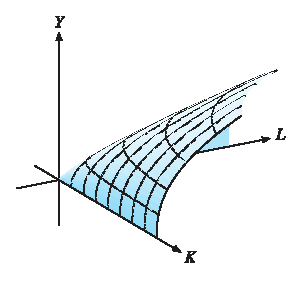
\includegraphics[width=\linewidth]{figure1}\label{fig:1}
			\caption{Gráfica de la función de producción Cobb-Douglas.}
		\end{minipage}
		\hfill
		\begin{minipage}[c]{0.4\linewidth}
			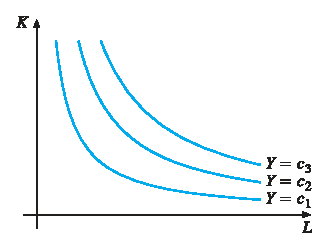
\includegraphics[width=\linewidth]{figure2}\label{fig:2}
			\caption{Isocuantas de la función de producción Cobb-Douglas.}
		\end{minipage}
	\end{figure}
\end{example}
% pag. 428
\begin{example}[Funciones $n$--lineales y $\log$--lineales]
	\leavevmode
	\begin{enumerate}
		\item\label{item:a} La demanda del azúcar en los Estados Unidos durante el período 1929--1936 fue estimado para ser descrito, aproximadamente, por la fórmula \[ x=108.83-6.0294p+0.164w-0.4217t \] donde $x$ es la demanda del azúcar, $p$ es su precio, $w$ es un índice de producción y $t$ es el año (donde $t=0$ corresponde a 1929).
		\item\label{item:b} La siguiente fórmula es una estimación para la demanda de cerveza en el Reino Unido: \[ x=1.058{x}^{0.136}_{1}{x}^{-0.727}_{2}{x}^{0.914}_{3}x^{0.816}_{4}. \]
		Aquí la cantidad demandada, $x$, es una función de cuatro variables: $x_{1}$, el ingreso per cápita, $x_{2}$, el precio de la cerveza, $x_{3}$, índice general de precios de productos básicos y $x_{4}$, la fuerza de la cerveza.
	\end{enumerate}
\end{example}
Las funciones más simples en el ejemplo anterior es la única en la parte~\eqref{item:a}. Las variables $p$, $w$ y $t$ ocurren solo cuando a la primera potencia, y ellas son multiplicadas por constantes, no por cada otra. Tales funciones son llamadas \emph{lineales}. En general
\begin{equation}
f\left(x_{1},x_{2},\ldots,x_{n}\right)=a_{1}x_{1}+a_{2}x_{2}+\cdots+a_{n}x_{n}+b
\end{equation}
donde $a_{1},a_{2},\ldots,a_{n}$ y $b$ son constantes, es una \emph{función lineal} en $n$ variables.

La función en la parte~\eqref{item:b} del ejemplo  es un caso especial de la función general de Cobb-Douglas
\begin{equation}\label{eq:cobbgeneralized}
F\left(x_{1},x_{2},\ldots,x_{3}\right)=A{x}^{a_{1}}_{1}{x}^{a_{2}}_{2}\cdots{x}^{a_{n}}_{n}
\end{equation}
donde $A>0$, $a_{1},\ldots,a_{n}$ son constantes, definidas para $x_{1}>0,x_{2}>0,\ldots x_{n}>0$. Note que al tomar el logaritmo natural a cada lado de~\eqref{eq:cobbgeneralized} resulta
\begin{equation}
\ln F=\ln A+a_{1}\ln x_{1}+a_{2}\ln x_{2}+\cdots+a_{n}\ln x_{n}.
\end{equation}
Esto muestra que la función de Cobb-Douglas es $\log$--lineal, ya que $\ln F$ es una función lineal para $\ln x_{1},\ln x_{2},\ldots,\ln x_{n}$.
% arara: lualatex: { draft: yes }
% arara: lualatex: { draft: yes }
% arara: pythontex
% !arara: biber
% arara: lualatex: { draft: yes }
% arara: lualatex: {
% arara: --> shell: yes,
% arara: --> synctex: yes,
% arara: --> interaction: batchmode
% arara: --> }
% arara: clean: {
% arara: --> extensions:
% arara: --> ['log','aux','out','pytxcode','synctex.gz','toc','bbl','bcf','blg', 'run.xml']
% arara: --> }
% arara: lualatex: { draft: yes }
% arara: lualatex: { draft: yes }
% arara: pythontex
% !arara: biber
% arara: lualatex: { draft: yes }
% arara: lualatex: {
% arara: --> shell: yes,
% arara: --> synctex: yes,
% arara: --> interaction: batchmode
% arara: --> }
% arara: clean: {
% arara: --> extensions:
% arara: --> ['log','aux','out','pytxcode','synctex.gz','toc','bbl','bcf','blg', 'run.xml']
% arara: --> }
% arara: lualatex: { draft: yes }
% arara: lualatex: { draft: yes }
% arara: pythontex
% !arara: biber
% arara: lualatex: { draft: yes }
% arara: lualatex: {
% arara: --> shell: yes,
% arara: --> synctex: yes,
% arara: --> interaction: batchmode
% arara: --> }
% arara: clean: {
% arara: --> extensions:
% arara: --> ['log','aux','out','pytxcode','synctex.gz','toc','bbl','bcf','blg', 'run.xml']
% arara: --> }
\input{cobb-douglas.tex.preamble}
\begin{document}

\maketitle
\include{./contents/spanish/abstract}

\tableofcontents

\include{./contents/spanish/introduction}
\include{./contents/spanish/cobb-douglas}
\include{./contents/spanish/solow}
\include{./contents/spanish/inada}
\include{./contents/spanish/models}
\include{./contents/spanish/deduction}
\include{./contents/spanish/understandingsolow}
\include{./contents/spanish/crecimiento}
%\include{./contents/spanish/codification}
%\include{./contents/spanish/sympying}
%\include{./contents/spanish/references}

\appendix

%\include{./contents/spanish/performance}
%\include{./contents/spanish/linearregression}

\vfill
\begin{flushright}
Facultad de Ciencias, \today.
\end{flushright}

\include{./contents/english/abstract}

\tableofcontents

\vfill
\begin{flushright}
Science department, \today.
\end{flushright}

\end{document}
\begin{document}

\maketitle
\selectlanguage{spanish}

\begin{abstract}
La función de producción Cobb-Douglas es un enfoque neoclásico para estimar la función de producción de un país y proyectar de esta manera su crecimiento económico esperado. Para representar las relaciones entre la producción obtenida se utiliza las variaciones de los insumos como el capital ($K$) y el trabajo ($L$), a los que más tarde se añadió la tecnología, llamada también productividad total de los factores ($PTF$). Es una función de producción frecuentemente utilizada en Economía.
%https://assets.aeaweb.org/asset-server/files/9434.pdf

El origen de la función Cobb-Douglas se encuentra en la observación empírica de la distribución de la renta nacional total de Estados Unidos entre el capital y el trabajo. De acuerdo a lo que mostraban los datos, la distribución se mantenía relativamente constante a lo largo del tiempo. Concretamente el trabajo se llevaba un 70\% y el capital un 30\%. De esta forma, la función Cobb-Douglas representa una relación en donde las proporciones de trabajo y capital con respecto al producto total son constantes.%\pygment{python}{module}
\end{abstract}

\tableofcontents

\section{Introducción}

Este proyecto hace referencia a la función de producción de Cobb-Douglas, siendo este publicado en \cite{Douglas1976} 1928 por \citeauthor{Douglas1976}, quienes realizaron un estudio en el que se modeló el crecimiento de la economía estadounidense. Para este proyecto se desarrollará una aplicación con una base de datos como un caso particular, pero previo a su aplicación, se realizará una posible forma de cómo Charles Cobb y Paul Douglas llegaron a la formulación algebraica de la función. Al finalizar, se comparará la solución exacta de la ecuación con la obtenida por el método de mínimos cuadrados.

\subsection{Función de producción de Cobb-Douglas}

Para el análisis matemático de la función, es necesario describir los factores involucrados en el modelo.

\subsection{Función de producción}

Es la relación entre las cantidades máximas de productos que una empresa puede fabricar mediante el uso de diversas cantidades de insumos. Las múltiples funciones de producción están representadas por la combinación de factores de insumo (tecnología, capital, trabajo entre otros). Una función de producción se expresa como la ecuación~\eqref{eq:production} siguiente:
\begin{equation}\label{eq:production}
P=f(K,L,I)
\end{equation}
donde:
\begin{itemize}
	\item $P$ es la cantidad de producción.
	\item $K,L,I$ son los insumos.
\end{itemize}

\section{El proyecto}

En esta sección explicaré los detalles de mi proyecto y su visión. Espero que esta estructura se mejore considerablemente bajo la guía de mi mentor.

\subsection{Cobb-Douglas y la función de producción ACMS}

Partiendo de la función Cobb-Douglas
\begin{equation}%\label{eq:1}
Y = bL^{k}C^{1-k},
\end{equation}
donde:
\begin{itemize}
	\item $b$ representa el factor total de productividad,
	\item $Y$ la producción total,
	\item $L$ el trabajo,
	\item $C$ el capital.
\end{itemize}
Esta función fue generalizada siendo expresada de la manera siguiente:
\begin{equation}%\label{eq:2}
f = \gamma{x}_{1}^{\alpha_{1}}\cdots x_{n}^{\alpha_{n}},
\end{equation}
donde $\gamma$ es una constante positiva y $\alpha_{1},\ldots,\alpha_{n}$ son constantes no cero.

Se dice que una función de producción $f$ es $d$--homogénea o homogénea de degradación $d$, si:
\begin{equation}%\label{eq:3}
f\left(tx_{1},\ldots,tx_{n}\right) = t^{d}f\left(x_{1},\ldots,x_{n}\right),
\end{equation}
Se mantiene para cada $t\in\mathbb{R}$ en la función previamente definida.

Una función \emph{homogénea de degradación uno} es llamado como \emph{linealmente homogéneo}.

Si $d>1$, la función homogénea mostrará un crecimiento a escala, caso contrario cuando $d<1$ mostrará un decrecimiento a escala.

Arrow, Chenery, Minhas y Solow(ACMS) introdujeron una función de producción de dos factores:
\begin{equation}%\label{eq:4}
Q=F\cdot(aK^r + (1-a)L^r)^{1/r},
\end{equation}
donde:
\begin{itemize}
	\item $Q$ representa el resultado,
	\item $F$ el factor de producción,
	\item $a$ el parámetro compartido,
	\item $k,L$ los factores de producción primario,
	\item $r=\left(s-1\right)/s$ , $s=1/\left(1-r\right)$ como la substitución de elasticidad.
\end{itemize}

La función de producción generalizada de ACMS se define:
\begin{equation}\label{eq:5}
f\left(x\right) = \gamma\sum_{i=1}^{n} ({{a}_{i}^{p}x_{i}^{p}})^{d/p},x=\left(x_{1},\ldots,x_{n}\right)\in D\subset\mathbb{R}_{+}^{n},
\end{equation}
con $a_{1},\ldots,a_{n},\gamma,p\neq0$, donde $d$ es la degradación de homogeneidad.

Cabe resaltar que la \emph{función de producción homotética} tiene la siguiente expresión como una función de producción:
\begin{equation}\label{eq:6}
f(x) = F\left(h(x_1,\ldots,x_n\right),
\end{equation}
donde F es una función estrictamente creciente y $h\left(x_1,\ldots,x_n\right)$ es una función homogénea de cualquier degradación d. La \emph{función de producción homotética} de la forma:
\begin{equation}\label{eq:7}
f\left(x\right) = \gamma\sum_{i=1}^{n} ({{a}_{i}^{p}x_{i}^{p}})^{d/p},\quad(\text{resp.},\quad f(x)=F(x_{1}^{\alpha_1}\cdots x_{n}^{\alpha_n}),
\end{equation}
es llamada \emph{función de producción ACMS generalizada homotética}.

\subsection{Breve descripción}

Si $f$ es una función de dos variables, a menudo dejamos que una letra como $z$ denote el valor de $f$ en el punto $\left(x,y\right)$, así $z=f\left(x,y\right)$. Entonces llamaremos a $x$ e $y$ las \emph{variables independientes}, o los \emph{argumentos} de $f$, mientras que $z$ es llamada la \emph{variable independiente}, porque el valor $z$, en general, depende de los valores $x$ e $y$. El dominio de la función $f$ es entonces el conjunto de todos los posibles pares de variables independientes, mientras que su \emph{rango} es el conjunto de valores correspondientes de la variable dependientes. En economía, $x$ e $y$ son llamadas las variables \emph{exógenas}, mientras que $z$ es la variable \emph{endógena}.

Una función de dos variables que aparecen en muchos modelos económicos es
\begin{equation}\label{eq:cobb-douglas}
F\left(x,y\right)=Ax^{a}y^{b}
\end{equation}
donde $A$, $a$ y $b$ son constantes. Usualmente, uno asume que $F$ es definida solo para $x>0$ e $y>0$.

A función de la forma~\eqref{eq:cobb-douglas} es generalmente llamada la \emph{función de Coubb-Douglas}. Se usa con mayor frecuencia para describir ciertos procesos de producción. Entonces $x$ e $y$ son llamados \emph{factores de entrada}, mientras que $F\left(x,y\right)$ es el número de unidades producidas, o la \emph{salida}. En este caso $F$ es llamada la \emph{función de producción}.

%\subsubsection{Defining \pygment{python}{ImageSet} Union for Trigonometric Equation Solver}%\protect||

% TODO: Page 276.
\begin{example}[Elasticidad de sustitución constante]
	Considere la ``elasticidad de sustitución constante'', o la función \textsc{CES}
	\begin{equation}
	F\left(K,L\right)=A\left(aK^{-\rho}+\left(1-a\right)L^{-\rho}\right)^{-1/\rho}
	\end{equation}
	donde $A>0$, $K>0$, $L>0$, $a\in\left(0,1\right)$, y $\rho\neq 0$. Manteniendo $A,K,L$ y $a$ fijos, aplique la regla de L'H\^{o}pital a $z=\ln\left[F\left(K,L\right)/A\right]$  cuando $\rho\to0$ con el fin de mostrar que $F\left(K,L\right)$ converge a la función de Cobb-Douglas $AK^{a}L^{1-a}$.
\end{example}

\begin{proof}[Solución]
	Obtenemos \[ z=\ln{\left(aK^{-\rho}+\left(1-a\right)L^{-\rho}\right)}^{-1/\rho}=-\ln\left(aK^{-\rho}+\left(1-a\right)L^{-\rho}\right)/\rho\to\frac{0}{0}\text{ cuando }\rho\to0. \] Ya que $\left(\mathrm{d}/\mathrm{d}\rho\right)K^{-\rho}=-K^{-\rho}\ln K$ y $\left(\mathrm{d}/\mathrm{d}\rho\right)L^{-\rho}=-L^{-\rho}\ln L$, aplicando la regla de L'H\^{o}pital da
	\begin{align*}
	\lim_{\rho\to0}z
	&=\lim_{\rho\to0}\left[\frac{aK^{-\rho}\ln K + \left(1-a\right)L^{-\rho}\ln L}{aK^{-\rho}+\left(1-a\right)L^{-\rho}}\right]\\
	&=a\ln K+\left(1-a\right)\ln L\\
	&=\ln K^{a}L^{1-a}.
	\end{align*}
	Por lo tanto, $e^{z}\to K^{a}L^{1-a}$. De la definición de $z$, se sigue que $F\left(K,L\right)\to AK^{a}L^{1-a}$ cuando $\rho\to0$.
\end{proof}

%pag. 408-409
\begin{example}[Función de Cobb-Douglas]
	Una función de dos variables que aparece en muchos modelos económicos es
	\begin{equation}\label{eq:cobb}
	F\left(x,y\right)=Ax^{a}y^{b}
	\end{equation}
	donde $A$, $a$ y $b$b son constantes. Usualmente, uno asume que $F$ está definida sola pora $x>0$ e $y>0$.

	Una función $F$ de la forma~\eqref{eq:cobb} es generalmente llamada la \emph{función de Cobb-Douglas}\footnote{La función en~\eqref{eq:cobb} es llamada en honor a los investigadores americanos C.W.Cobb y P.H.Douglas, quien aplicaron esto, con  $a+b=1$, en un articulo científico que aparecio en 1927 en la estimacion de una función de producción. Sin embargo, deberia correctamente ser llamada la ``función de Wicksell'', porque el economista sueco K.Wicksell(1851-1926) introdujo tales funciones de producción antes de 1900.}. Con frecuencia es usada para describir ciertos procesos productivos. Así, $x$ e $y$ son llamados los \emph{factores de entrada}, mientras que $F\left(x,y\right)$ es el número de unidades producidas, o la \emph{salida}. En este caso, $F$ es llamada una \emph{función de producción}.
\end{example}

\begin{example}
	Suponga que $F\left(K,L\right)$ modela la producción de una empresa cuando sus entradas son capital y labor, respectivamente $K$ y $L$. Una curva de nivel por esta función de producción es una curva en el plano $KL$ dado por $F\left(K,L\right)=Y_{o}$, donde $Y_{0}$ es una constante. Esta curva es llamada una \emph{isocuanta}, que significa ``igual cantidad''. Para una función de Cobb-Douglas, $F\left(K,L\right)=AK^{a}L^{b}$, con $a+b<1$ y $A>0$, las figuras~\ref{fig:1} y~\ref{fig:2}, respectivamente, muestra una parte de la gráfica cerca del origen, y tres de las isocuantas.
	
	\begin{figure}[ht!]
		\begin{minipage}[c]{0.4\linewidth}
			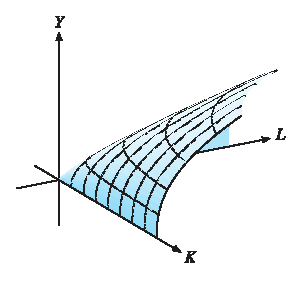
\includegraphics[width=\linewidth]{figure1}\label{fig:1}
			\caption{Gráfica de la función de producción Cobb-Douglas.}
		\end{minipage}
		\hfill
		\begin{minipage}[c]{0.4\linewidth}
			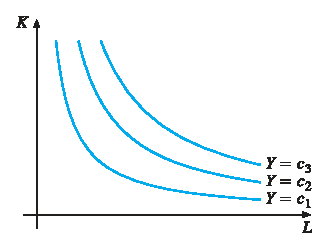
\includegraphics[width=\linewidth]{figure2}\label{fig:2}
			\caption{Isocuantas de la función de producción Cobb-Douglas.}
		\end{minipage}
	\end{figure}
\end{example}
% pag. 428
\begin{example}[Funciones $n$--lineales y $\log$--lineales]
	\leavevmode
	\begin{enumerate}
		\item\label{item:a} La demanda del azúcar en los Estados Unidos durante el período 1929--1936 fue estimado para ser descrito, aproximadamente, por la fórmula \[ x=108.83-6.0294p+0.164w-0.4217t \] donde $x$ es la demanda del azúcar, $p$ es su precio, $w$ es un índice de producción y $t$ es el año (donde $t=0$ corresponde a 1929).
		\item\label{item:b} La siguiente fórmula es una estimación para la demanda de cerveza en el Reino Unido: \[ x=1.058{x}^{0.136}_{1}{x}^{-0.727}_{2}{x}^{0.914}_{3}x^{0.816}_{4}. \]
		Aquí la cantidad demandada, $x$, es una función de cuatro variables: $x_{1}$, el ingreso per cápita, $x_{2}$, el precio de la cerveza, $x_{3}$, índice general de precios de productos básicos y $x_{4}$, la fuerza de la cerveza.
	\end{enumerate}
\end{example}
Las funciones más simples en el ejemplo anterior es la única en la parte~\eqref{item:a}. Las variables $p$, $w$ y $t$ ocurren solo cuando a la primera potencia, y ellas son multiplicadas por constantes, no por cada otra. Tales funciones son llamadas \emph{lineales}. En general
\begin{equation}
f\left(x_{1},x_{2},\ldots,x_{n}\right)=a_{1}x_{1}+a_{2}x_{2}+\cdots+a_{n}x_{n}+b
\end{equation}
donde $a_{1},a_{2},\ldots,a_{n}$ y $b$ son constantes, es una \emph{función lineal} en $n$ variables.

La función en la parte~\eqref{item:b} del ejemplo  es un caso especial de la función general de Cobb-Douglas
\begin{equation}\label{eq:cobbgeneralized}
F\left(x_{1},x_{2},\ldots,x_{3}\right)=A{x}^{a_{1}}_{1}{x}^{a_{2}}_{2}\cdots{x}^{a_{n}}_{n}
\end{equation}
donde $A>0$, $a_{1},\ldots,a_{n}$ son constantes, definidas para $x_{1}>0,x_{2}>0,\ldots x_{n}>0$. Note que al tomar el logaritmo natural a cada lado de~\eqref{eq:cobbgeneralized} resulta
\begin{equation}
\ln F=\ln A+a_{1}\ln x_{1}+a_{2}\ln x_{2}+\cdots+a_{n}\ln x_{n}.
\end{equation}
Esto muestra que la función de Cobb-Douglas es $\log$--lineal, ya que $\ln F$ es una función lineal para $\ln x_{1},\ln x_{2},\ldots,\ln x_{n}$.
% arara: lualatex: { draft: yes }
% arara: lualatex: { draft: yes }
% arara: pythontex
% !arara: biber
% arara: lualatex: { draft: yes }
% arara: lualatex: {
% arara: --> shell: yes,
% arara: --> synctex: yes,
% arara: --> interaction: batchmode
% arara: --> }
% arara: clean: {
% arara: --> extensions:
% arara: --> ['log','aux','out','pytxcode','synctex.gz','toc','bbl','bcf','blg', 'run.xml']
% arara: --> }
\input{cobb-douglas.tex.preamble}
\begin{document}

\maketitle
\include{./contents/spanish/abstract}

\tableofcontents

\include{./contents/spanish/introduction}
\include{./contents/spanish/cobb-douglas}
\include{./contents/spanish/solow}
\include{./contents/spanish/inada}
\include{./contents/spanish/models}
\include{./contents/spanish/deduction}
\include{./contents/spanish/understandingsolow}
\include{./contents/spanish/crecimiento}
%\include{./contents/spanish/codification}
%\include{./contents/spanish/sympying}
%\include{./contents/spanish/references}

\appendix

%\include{./contents/spanish/performance}
%\include{./contents/spanish/linearregression}

\vfill
\begin{flushright}
Facultad de Ciencias, \today.
\end{flushright}

\include{./contents/english/abstract}

\tableofcontents

\vfill
\begin{flushright}
Science department, \today.
\end{flushright}

\end{document}
\section{Introducción}
Cualquier teoría depende de supuestos que no son del todo ciertos. Eso es lo que lo hace teoría. El arte de teorizar con éxito es hacer los supuestos simplificadores inevitables de tal manera que los resultados finales no sean muy sensibles. Una suposición ``crucial'' es una de las cuales las conclusiones dependen sensiblemente, y es importante
que los supuestos cruciales sean razonablemente realistas. Cuando los resultados de una teoría parecen fluir específicamente de una suposición crucial especial, entonces, si la suposición es dudosa, los resultados son sospechosos.

Deseo argumentar que algo así es cierto en el modelo de crecimiento económico Harrod--Domar. La característica y poderosa conclusión de la línea de pensamiento Harrod--Domar es que incluso para el largo plazo, el sistema económico está en el mejor de los casos equilibrado sobre el filo del cuchillo del equilibrio del crecimiento. ¿Eran las magnitudes de los parámetros clave --la relación de ahorro, la relación capital-producto, la tasa de aumento de la mano de obra--si se deslizara un poco desde el punto muerto, la consecuencia sería un desempleo creciente o una inflación prolongada. En términos de Harrod, la cuestión crítica del equilibrio se reduce a una comparación entre la tasa natural de crecimiento que depende, en la ausencia del cambio tecnológico, en el aumento de la fuerza laboral, y la tasa de crecimiento garantizada que depende de los hábitos de ahorro e inversión de los hogares y las empresas.

Pero esta oposición fundamental de tasas garantizadas y naturales al final resulta que parte del supuesto crucial de que la producción tiene lugar en condiciones de \emph{proporciones fijas}. No hay posibilidad de sustituir mano de obra por capital en producción. Si esta suposición se abandona, la noción del filo de cuchillo de equilibrio inestable parece ir con eso. De hecho, no es sorprendente que una rigidez tan grave en una parte del sistema implique falta de flexibilidad en otro.

Una característica notable del modelo Harrod--Domar es que estudia constantemente los problemas a largo plazo con las herramientas de corto plazo habitual. Normalmente se piensa en el largo plazo como el dominio del análisis neoclásico, la tierra del margen. En cambio Harrod y Domar hablan del largo plazo en términos del multiplicador, el acelerador, ``el'' coeficiente de capital. La mayor parte de este documento está dedicado a un modelo de crecimiento a largo plazo que acepta todos los supuestos de Harrod--Domar excepto el de proporciones fijas. En cambio supongo que la única mercancía compuesta es producida por trabajo y capital bajo las condiciones neoclásicas estándar. La adaptación del sistema a una tasa de incremento de la fuerza laboral dada de manera exógena se calcula en algún detalle, para ver si aparece la inestabilidad de Harrod. Las reacciones de interés precio-salario juegan un papel importante en este proceso de ajuste neoclásico, por lo que también se analizan. Luego, algunos de los otros rígidos supuestos se relajan ligeramente para ver qué cambios cualitativos resultan: se permite un cambio tecnológico neutral y un interés elástico horario de ahorro. Finalmente, las consecuencias de ciertas relaciones y rigideces más ``keynesianas'' son brevemente consideran.

\section{Un modelo de crecimiento a largo plazo}
Solo hay una mercancía, la producción como un todo, cuya tasa de producción se designa $Y\left(t\right)$. Así podemos hablar inequívocamente del ingreso real de la comunidad. Parte de cada salida instantánea es consumida y el resto se ahorra e invierte. La fracción de la salida ahorrada es una constante $s$, de modo que la tasa de ahorro es $sY\left(t\right)$. El stock de capital de la comunidad $K\left(t\right)$ toma la forma de una acumulación de la mercancía compuesta. La inversión neta es solo la tasa de
aumento de este capital social $\mathrm{d}K/\mathrm{d}t$ o $\dot{K}$, por lo que tenemos la identidad básica en cada instante de tiempo:
\begin{equation}\label{eq:first}
\dot{K}=sY
\end{equation}
La salida es producida con la ayuda de dos factores de producción, capital y trabajo, cuya tasa de ingreso es $L\left(t\right)$. Las posibilidades tecnológicas son representadas por una función de producción.
\begin{equation}\label{eq:second}
Y=F\left(K,L\right)
\end{equation}
La salida es entendida como la salida neta después de hacer buena la depreciación del capital. Sobre la producción, todo lo que diremos en este momento es que muestra rendimientos constantes a escala. Por lo tanto, la función de producción es homogénea de primer grado. Esto equivale a asumir que no existe un recurso escaso no aumentable como la tierra. Retornos de escala constante parece la suposición natural para hacer en una teoría de crecimiento. El caso de tierras escasas conduciría a rendimientos decrecientes a
escala en capital y trabajo y el modelo se volvería más Ricardiano.

Insertando~\eqref{eq:second} en~\eqref{eq:first} obtenemos
\begin{equation}\label{eq:third}
\dot{K}=sF\left(K,L\right).
\end{equation}
Este es una ecuación con dos incógnitas. Una primera manera de acercarse al sistema sería agregar una ecuación de demanda de trabajo: la productividad física del trabajo marginal es igual a la tasa salarial real; y una ecuación de oferta de trabajo. Este último podría tomar la forma general de hacer trabajo proporcionar una función del salario real, o más clásico de poner el salario real igual a un nivel de subsistencia convencional. En cualquier caso serían tres ecuaciones en las tres incógnitas $K$, $L$, salario real.

En cambio, procedemos más en el espíritu del modelo Harrod. Como un resultado exógeno del crecimiento de la población, la fuerza laboral aumenta a una tasa relativa constante $n$. En ausencia de cambio tecnológico, $n$ es la tasa natural de crecimiento de Harrod. Así:
\begin{equation}\label{eq:fourth}
L\left(t\right)=L_{0}e^{nt}
\end{equation}
En~\eqref{eq:third} $L$ representa el empleo total; en~\eqref{eq:fourth} $L$ representa la oferta de trabajo disponible. Al identificar los dos estamos asumiendo que el empleo se mantiene perpetuamente. Cuando insertamos~\eqref{eq:fourth} en~\eqref{eq:third} obtenemos
\begin{equation}\label{eq:fifth}
\dot{K}=sF\left(K,L_{0}e^{nt}\right)
\end{equation}
tenemos la ecuación básica que determina el camino temporal de la acumulación del capital que debe ser serguida si todas los trabajos disponibles están empleados.

Alternativamente,~\eqref{eq:fourth} puede ser visto como una curva de oferta de mano de obra. Eso dice que la fuerza laboral que crece exponencialmente se ofrece para un empleo completamente inelástico. La curva de oferta de trabajo es una línea vertical que se mueve hacia la derecha en el tiempo a medida que la fuerza laboral crece de acuerdo
para~\eqref{eq:fourth}. Luego, la tasa salarial real se ajusta para que toda la mano de obra disponible sea empleado, y la ecuación de productividad marginal determine la tasa salarial que realmente gobernará.

En resumen,~\eqref{eq:fifth} es una ecuación diferencial con la única variable $K\left(t\right)$. Su solución da el único perfil de tiempo del capital social de la comunidad que empleará plenamente la mano de obra disponible. Una vez que nosotros conozca el camino temporal del stock de capital y el de la fuerza laboral, podemos calcular desde la función de producción la ruta de tiempo correspondiente de salida real. La ecuación de productividad marginal determina la trayectoria temporal del salario real. También hay una suposición involucrada de pleno empleo del stock de capital disponible. En cualquier punto de tiempo en que el stock de capital preexistente (el resultado de una acumulación previa) se suministra de manera inelástica. Por lo tanto, existe una ecuación de productividad marginal similar para el capital que determina el alquiler real por unidad de tiempo para los servicios de capital social. El proceso puede ser visto de esta manera: en cualquier momento la oferta laboral disponible está dado por~\eqref{eq:fourth} y el stock de capital disponible también es un dato. Ya que el rendimiento real de los factores se ajustará para lograr el pleno empleo de trabajo y capital podemos usar la función de producción~\eqref{eq:second} para encontrar la tasa actual de salida. Entonces la propensión a ahorrar nos dice cuánto de la producción neta se ahorrará e invertirá. Por eso conocemos la acumulación del capital neta durante el período actual. Agregado al stock ya acumulado, esto da el capital disponible para el próximo período, y todo el proceso puede repetirse.
\section{Posibles patrones de crecimiento}
Para ver si siempre existe una ruta de acumulación de capital consistente con cualquier tasa de crecimiento de la fuerza laboral, debemos estudiar la ecuación diferencial~\eqref{eq:fifth} por la naturaleza cualitativa de sus soluciones. Naturalmente sin especificar la forma exacta de la función de producción no podemos esperar encontrar la solución exacta. Pero ciertas propiedades amplias son sorprendentemente fáciles de aislar, incluso gráficamente.

Para ello, introducimos una nueva variable $r=\frac{K}{L}$, la relación de capital al trabajo Por lo tanto, tenemos $K=rL=rL_{0}e^{nt}$. Diferenciando con respecto al tiempo que tenemos
\begin{equation}
\dot{K}=L_{0}e^{nt}r^{\prime}+nrL_{0}e^{nt}.
\end{equation}
Reemplazando esto en~\eqref{eq:fifth}: \[ \left(\dot{r}+nr\right)L_{0}e^{nt}=sF\left(K,L_{0}e^{nt}\right). \] Pero debido al retorno de escala constante podemos dividir ambas variales en $F$ por $L=L_{0}e^{nt}$, no obstante, multiplicamos $F$ por el mismo factor. Así \[ \left(\dot{r}+nr\right)L_{0}e^{nt}=sLe^{nt}F\left(\frac{K}{L_{0}e^{nt}},1\right) \] y dividiendo el factor común llegamos finalmente a
\begin{equation}\label{eq:sixth}
\dot{r}=sF\left(r,1\right)-nr.
\end{equation}
Aquí tenemos una ecuación diferencial que involucra solamente la relación capital-trabajo.

Esta ecuación fundamental se puede alcanzar menos formalmente. Como $r=\frac{K}{L}$, la tasa de cambio relativa de $r$ es la diferencia entre las tasas relativas de cambio de $K$ y $L$. Eso es: \[ \frac{\dot{r}}{r}=\frac{\dot{K}}{K}-\frac{\dot{L}}{L}. \] Ahora primero que nada $\frac{\dot{L}}{L}=n$. En segundo lugar, $\dot{K}=sF\left(K,L\right)$. Haciendo estas substituciones: \[ \dot{r}=r\frac{sF\left(K,L\right)}{K}-nr. \] Ahora divida $L$ de $F$ como antes, note que que $\frac{L}{K}=\frac{1}{r}$ y obtenemos~\eqref{eq:sixth} nuevamente.

La función $F\left(r,1\right)$ que aparece en~\eqref{eq:sixth} es fácil de interpretar. Esta es la curva del producto total cuando varían las cantidades $r$ de capital con una unidad de trabajo. Alternativamente, da salida por trabajador como una función de capital por trabajador. Así~\eqref{eq:sixth} establece que la tasa del cambio de la relación capital-trabajo es la diferencia de dos términos, uno representando el incremento de capital y uno el incremento de trabajo.

Cuando $\dot{r}=0$, la relación capital-trabajo es una constante, y el capital existente debe expandirse al mismo ritmo que la fuerza laboral, es decir, $n$.

(La tasa de crecimiento garantizada, garantizada por la tasa real apropiada de retorno al capital, es igual a la tasa natural.) En la Figura I, el rayo que pasa por el origen con pendiente $n$ representa la función $nr$. La otra curva es la función $sF\left(r,1\right)$. Aquí se dibuja para pasar por el origen y convexo hacia arriba: sin salida a menos que ambas entradas sean positivas, y la disminución de la productividad marginal del capital, como sería el caso, por ejemplo, con la función Cobb-Douglas. En el punto de intersección $nr=sF\left(r,1\right)$ y $\dot{r}=0$. Si la relación capital-trabajo $r^{\ast}$ debe establecerse, se mantendrá, y el capital y
el trabajo crecerá de allí en adelante en proporción. Por la constante retornos a escala

\newpage
Formalmente, una función de producción se define para tener:
\begin{itemize}
	\item Constante retorno a escala si (para cualquier constante $a$ es mayor que $0$) $F\left(aK,aL\right)=aF\left(K,L\right)$ (Función $F$ es homogénea de grado $1$).
	\item Retornos a escala crecientes si (para cualquier constante mayor que $1$) $F\left(aK,aL\right)>aF\left(K,L\right)$.
	\item Retornos a escala decrecientes si (para cualquier constante $a$ mayor que $1$) $F\left(aK,aL\right)<aF\left(K,L\right)$.
\end{itemize}
donde $K$ y $L$ son factores de producción--capital y trabajo, respectivamente.

En una configuración más general, para procesos de producción de múltiples entradas y múltiples salidas, se puede suponer que la tecnología se puede representar a través de algún conjunto de tecnología, llámelo $T$ que debe satisfacer algunas condiciones de regularidad de la teoría de la producción. En este caso, la propiedad de retorno de escala constante es equivalente a decir que el conjunto tecnológico es un cono, es decir, satisface la propiedad $aT=T$, $\forall a>0$. A su vez, si hay una función de producción que describirá el conjunto de tecnología $T$, deberá ser homogéneo de grado $1$.


\begin{definition}[Rendimiento de escala]
	La forma funcional de Cobb-Douglas tiene una constante retorno de escala cuando la suma de sus exponentes es $1$. En este caso, la función es
	\begin{equation}
	F\left(K,L\right)=AK^{b}L^{1-b}
	\end{equation}
	donde $A>0$ y $0<b<1$. Así \[ F\left(aK,aL\right)=A{\left(ak\right)}^{b}{\left(aL\right)}^{1-b}=Aa^{b}a^{1-b}K^{b}L^{1-b}=aAK^{b}L^{1-b}=aF\left(K,L\right). \] Aquí como entrada usamos todas las escalas por un factor multiplicador $a$, la salida también escala por $a$ y así existen constantes de retorno de escala.
	
	Pero, si la función de producción de Cobb-Douglas tiene su forma general
	\begin{equation}
	F\left(K,L\right)=AK^{b}L^{c}
	\end{equation}
	donde $0<b<1$ y $0<c<1$, entonces existen retornos crecientes si $b+c>1$, pero retornos decrecientes si $b+c<1$, dado que \[ F\left(aK,aL\right)=A{\left(aK\right)}^{b}{\left(aL\right)}^{c}=Aa^{b}a^{c}K^{b}L^{c}=a^{b+c}AK^{b}L^{c}=a^{b+c}F\left(K,L\right), \] que para $a>1$ es mayor que o menor que $aF\left(K,L\right)$ cuando $b+c$ es mayor o menor que uno.
\end{definition}

Hay dos clases especiales de funciones de producción que a menudo se analizan. La función de producción $Q=f\left(X_{1},X_{2},\ldots,X_{n}\right)$ se dice que es homogéneo de grado $m$, si se le da alguna constante positiva $k$, $f\left(kX_{1},kX_{2},\ldots,kX_{n}\right)=k^{m}f\left(X_{1},X_{2},\ldots, X_{n}\right)$. Si $m>1$, la función exhibe rendimientos crecientes a escala, y exhibe rendimientos decrecientes a escala si $m<1$. Si es homogéneo de grado $1$, exhibe rendimientos constantes a escala. La presencia de rendimientos crecientes significa que un aumento del uno por ciento en los niveles de uso de todas las entradas daría como resultado un aumento de más del uno por ciento en la producción; la presencia de rendimientos decrecientes significa que daría como resultado un aumento de producción de menos del uno por ciento. Los retornos constantes a escala son el caso intermedio. En la función de producción Cobb–Douglas mencionada anteriormente, los rendimientos a escala aumentan si $a_{1}+a_{2}+\cdots+a_{n}> 1$, disminuyendo si $a_{1}+a_{2}+\cdots+a_{n}<1$, y constante si $a_{1}+a_{2}+\cdots+a_{n}=1$.

Si una función de producción es homogénea y de grado uno, este a veces llamada ``linealmente homogénea''. Una función de producción linealmente homogénea con entradas capital y labor tienen las propiedades de que los productos físicos marginales y promedio tanto del capital como del trabajo pueden expresarse solamente como funciones de la relación capital-trabajo. Además, en este caso, si cada entrada se paga a una tasa igual a su producto marginal, los ingresos de la empresa se agotarán exactamente y no habrá ganancias económicas excesivas.

Las funciones homotéticas son funciones cuya tasa de sustitución técnica marginal (la pendiente de la isocuanta, una curva dibujada a través del conjunto de puntos en dicho espacio de trabajo-capital en el que se produce la misma cantidad de producción para combinaciones variables de las entradas) es homogénea de grado cero Debido a esto, a lo largo de los rayos que provienen del origen, las pendientes de las isocuantas serán las mismas. Las funciones homotéticas tienen la forma $F\left(h\left(X_{1},X_{2}\right)\right)$ donde $F(y)$ es una función monótona creciente (la derivada de $F\left(y\right)$ es positiva $\mathrm{d}F/\mathrm{d}y>0$, y la función $h\left(X_{1},X_{2}\right)$ es una función homogénea de cualquier grado.

La elasticidad de sustitución constante (CES), en economía, es una propiedad de algunas funciones de producción y funciones de utilidad.

Específicamente, este en un tipo particular de función agregado que combina dos o más tipos de productos de consumos, o dos o más tipos de entradas de producción dentro de un cantidad agregado. Esta función de agregación exhibe una elasticidad de sustitución constante.
\begin{definition}[Elasticidad de sustitución constante]
La función de producción CES es una función de producción neoclásica que muestra una elasticidad de sustitución constante. En otras palabras, la producción tecnológica tiene un porcentaje de cambio constante en factores (por ejemplo, trabajo y capital) proporcional debido al cambio porcentual en la tasa marginal de la sustitución técnica. Los dos factores (capital y trabajo) de la función de producción fue introducido por Solow y más tarde popularizado por Arrow, Chenery, Minhas y Solow es
\begin{equation}
Q=F\cdot{\left(a\cdot K^{\rho}+\left(1-a\right)\cdot L^{\rho}\right)}^{\frac{v}{\rho}}
\end{equation}
donde
\begin{itemize}
	\item $Q$ es la cantidad de salida,
	\item $F$ es el factor de productividad,
	\item $a$ es el parámetro forma,
	\item $K,L$ son las cantidades de los factores de producción primario (capital y trabajo)
	\item $\rho=\frac{\sigma-1}{\sigma}$ es el parámetro de sustitución,
	\item $\sigma=\frac{1}{1-\rho}$ es elasticidad de sustituación,
	\item $v$ es el grado de homogeneidad de la función de producción. Donde $v=1$ es el retorno de escala constante, $v<1$ es el retorno de escala decreciente y $v>1$ es el retorno de escala creciente.
\end{itemize}
Como su nombre lo sugiere, la función de producción CES exhibe una elasticidad de sustitución constante entre el capital y el trabajo. Leontief, linear y las funciones de Cobb-Douglas son casos especiales de la función de producción CES. Esto es,
\begin{itemize}
	\item Si $\rho$ se aproxima a $1$, tenemos una lineal o función de sustituto perfecto.
	\item Si $\rho$ se aproxima a cero en el límite, obtenemos la función de producción de Cobb-Douglas.
	\item Si $\rho$ se aproxima al menos infinito, obtenemos la Leontief o función de producción perfecta complementaria.
\end{itemize}
La forma general de la función de producción CES, con $n$ entradas, es
\begin{equation}
Q=F\cdot{\left[\sum_{i=1}^{n}a_{i}X^{r}_{i}\right]}^{\frac{1}{r}}
\end{equation}
donde
\begin{itemize}
	\item $Q$ es cantidad de salida
	\item $F$ es el factor de productividad
	\item $a_{i}$ es el parámetro forma de la entrada $i$, $\sum_{i=1}^{n}a_{i}=1$
	\item $X_{i}$ son las cantidades de los factores de producción, $i=1,2,\ldots,n$.
	\item $s=\frac{1}{1-r}$ es la elasticidad de sustitución.
\end{itemize}
\end{definition}
Extendiendo la forma función CES (Solow) para acomodar los múltiples factores de producción crea algunos problemas. Sin embargo, no existe una forma completamente general para hacer esto. Uzawa mostró que solo $n$ factores posibles de la función de producción $n>2$ con elasticidades de sustitución parciales constantes requiere o todas las elasticidades entre pares de factores son idénticas, o si alguna difiere, todo ellos deben ser igual a cada otra y todas las elasticidades restantes deben ser unitarias. Esto es verdad para cualquier función de producción. Esto significa el uso de la forma funcional CES para más dos factores significará general que no existe una elasticidad de sustitución entre todos los factores.

Las funciones CES anidades son comúnmente encontradas en los modelos de equilibrio parcial y equilibrio general. Diferentes anidamientos (niveles) permiten la introducción de las elasticidades de sustitución apropiadas.

\begin{definition}[Función de utilidad CES]
La misma forma funcional CES alcanza como una función de utilidad en la teoría del consumidor. Por ejemplo, si existen $n$ tipos de productos de consumos $x_{i}$, entonces el consumo agregado $X$ podría definirse usando el agregado CES:
\begin{equation}
X={\left[\sum_{i=1}^{n}a^{\frac{1}{s}}_{i}x^{\frac{s}{s-1}}_{i}\right]}^{\frac{s}{s-1}}
\end{equation}
Aquí nuevamente, los coeficientes $a_{i}$ son los parámetros forma y $s$ es la elasticidad de sustitución. Por lo tanto, los productos de consumo $x_{i}$ son perfectos sustitutos cuando $s$ se aproxima al infinito y complemento perfecto cuando $s$ se aproxima a cero. El agregado CES es también algunas veces llamado el \emph{agregador Armington}, el cual fue discutido por Armington (1969).

Las funciones de utilidad CES son un caso especial de las preferencias homotéticas.

El siguiente es un ejemplo de la función de utilidad CES para dos productos, $x$ e $y$ con igualdad compartidad:
\begin{equation}
u\left(x,y\right)={\left(x^{r}+y^{r}\right)}^{1/r}.
\end{equation}
La función expendidora en el caso es:
\begin{equation}
e\left(p_{x},p_{y},u\right)={\left(p^{r/\left(r-1\right)}_{x}+p^{r/\left(r-1\right)}_{y}\right)}^{\left(r-1\right)/r}\cdot u.
\end{equation}
La función de utilidad indirecta tiene su inversa:
\begin{equation}
v\left(p_{x},p_{y},I\right)={\left(p^{r/\left(r-1\right)}_{x}+p^{r/\left(r-1\right)}_{y}\right)}^{\left(1-r\right)/r}\cdot I.
\end{equation}
La funciones de demanda son:
\begin{align*}
x\left(p_{x},p_{y},I\right)
&=\frac{p^{1/\left(r-1\right)}_{x}}{p^{r/\left(r-1\right)}_{x}+p^{r/\left(r-1\right)}_{y}}\cdot I\\
y\left(p_{x},p_{y},I\right)
&=\frac{p^{1/\left(r-1\right)}_{y}}{p^{r/\left(r-1\right)}_{x}+p^{r/\left(r-1\right)}_{y}}\cdot I\\
\end{align*}
La función de utilidad CES es uno de los casos considerados por Dixit y Stiglitz (1977) en su estudio de la diversidad del producto optimal en el contexto de la competición monopolística.

Note que la diferencial entre la utilidad CES y la utilidad isoelástica: La función de utilidad CES es una función de utilidad ordinal que representa las preferencias sobre consumo seguro %TODO: Wikipedia https://en.wikipedia.org/wiki/Constant_elasticity_of_substitution
mientras que la función de utilidad isoelástica es una función de utilidad cardinal que representa en loterías. Una función de utilidad CES indirecta (dual) ha sido usado para derivar la marca de consistencia-utildidad de sistemas donde la demanda categórica son determinadas endógenamente por un multicategorizador, la función de utilidad CES indirecto. Esto también se ha muestro que las preferencias son autoduales y ambos son primales y duales % TODO:
podrían exhibir cualquier grado de convexidad.
\end{definition}
La existencia y la estabilidad relativa de un único crecimiento balanceado para modelos multisectoriales fueron establecidos por Solow y Samuelson bajo el supuesto de \emph{retorno de escala constante}. Ellos estudiaron dos tipos de sistemas de ecuaciones: el sistema de ecuación en \emph{diferencias} y el sistema de ecuación diferencial. Later Muth y Suit estudiaron el sistema formado bajo el supuesto de retorno de escala decreciente. El primer objetivo de este artículo es estudiar algún sistema de ecuación diferencial bajo los supuestos más débiles que los impuestos por Solow y Samuelson, pero que retenga el supuesto de \emph{retorno constante} de escala. El segundo objetivo es investigar cierto sistema de ecuación diferencial bajo el supuesto de \emph{retorno de escala decreciente}.

\subsection{Retorno de escala constante -- Caso general}
Nuestro sistema es expresado por las siguientes ecuaciones:
\begin{equation}
\dot{X}_{i}=H^{i}\left(X_{1},\ldots,X_{n}\right),\quad\left(i=1,\ldots,n\right).
\end{equation}
El sistema de arriba es modelo de crecimiento balanceado de Solow--Samuelson. Los $H^i$'s son definidos para cualquier $\left(X_{1},\ldots,X_{n}\right)\geq0$ y son asumidos que son continuas con respecto a cualquier variable y positivamente homogénea de grado uno. A lo largo del artículo, los $X_{i}$'s son restringidos a valores no negativos. Además, las funciones son solo definidas para valores no negativos. Esto es asumido que
\begin{equation}
H^{i}\text{ es no decreciente en todas las variables, excepto en }X^{i},
\end{equation}
y que
\begin{equation}
\left\{H^{1},\ldots,H^{n}\right\}\text{ es indescomponible}.
\end{equation}
Aquí la indescomposibilidad es definido como en Morishima. Esto es, para cualquier conjunto de índices $R=\left\{i_{i},\ldots,i_{r}\right\}$, las relaciones $X_{i}=X^{\prime}_{i}$ para $i\in R$ y $X_{l}<X^{\prime}_{l}$ para $l\notin R$ implica que existe por lo menos un $i\in R$ tal que $H^{i}\left(X_{1},\ldots,X_{n}\right)<H^{i}\left(X^{\prime}_{i},\ldots,X^{\prime}_{n}\right)$. Requerimos que $H^{i}$ sea no decreciente en $X_{j}$, para $j\neq i$, sin la restricción sobre la dependencia de $H^{i}$ sobre $X_{i}$. En contraste del supuesto de Solow y Samuelson que $H^{i}$ es creciente en todos los $X_{j}$.

Ddas sus supuestos y la homogeneidad de $H^{i}$ $\left(i=1,\ldots,n\right)$, este sigue que $H^{i}\geq0$ $(i=1,\ldots,n)$ para $X_{j}\geq0$ $(j=1,\ldots,n)$, y que, $H^{i}=0$  para todo $i$, si y solo si $X_{j}=0$ para todo $j$. En nuestro caso, sin embargo, $H^{i}$ no es necesariamente creciente en $X$. Por ello, no podemos obtener las propiedades mencionadas arriba. Así, asumimos ellos. Esto es, podemos asumir que
\begin{equation}
H^{i}\geq0\quad(i=1,\ldots,n)\text{ para }X_{j}\geq0\quad\left(j=1,\ldots,n\right).
\end{equation}
Entonces, de la indescomposabilidad y la homogeneidad de $H^{i}$, $H^{i}=0$ para todo $i$, si y solo si $X_{j}=0$ para todo $j$. Nuestro ánimo es probar el siguiente teorema.

\begin{theorem}
	Para el sistema de ecuaciones diferenciales, %TODO
	existe un único determinado positivo autovalor, estrictamente un único positivo autovector normalizado y así un único camino de crecimiento balanceado. Más aún, cualquier solución del camino del sistema relativamente se aproxima al camino de crecimiento balanceado.
\end{theorem}
\begin{proof}
Podemos mostrar por un procedimiento similar al de Solow y Samuelson sobre la existencia de un autovalor positivo $\lambda$ y un autovector no negativo, no nulo $V=\left(V_{1},V_{2},\ldots,V_{n}\right)$ tal que
\begin{align*}
\lambda V_{1}&=H^{1}\left(V_{1},\ldots,V_{n}\right),\\
&=\vdots\\
\lambda V_{n}&=H^{n}\left(V_{1},\ldots,V_{n}\right).
\end{align*}
Mostraremos que \emph{todas las componentes del autovector} $V$ \emph{son positivas}. Suponga que algunas componentes de $V$ son ceros. Sin pérdida de generalidad, podríamos suponer que \[ V_{i}=0\quad\text{para }i\leq r(<n), \] y \[ V_{i}>0\quad\text{ para }n\geq i>r. \] Entonces,
\begin{align*}
0&=H^{1}\left(0,\ldots0,V_{r+1},\ldots,V_{n}\right),\\
&=\vdots
0&=H^{r}\left(0,\ldots0,V_{r+1},\ldots,V_{n}\right),\\
0<\lambda V_{r+1}&=H^{r+1}\left(0,\ldots0,V_{r+1},\ldots,V_{n}\right),\\
&=\vdots
0<\lambda V_{n}&=H^{n}\left(0,\ldots0,V_{r+1},\ldots,V_{n}\right).
\end{align*}
Pero esto contradice la suposición de indescomposabilidad, así es fácilmente visto haciendo
\begin{align*}
R\equiv\left\{1,\ldots,r\right\},\\
\left(X_{1},\ldots,X_{r},X_{r+1},\ldots,X_{n}\right)
&\equiv\left(0,\ldots0,V_{r+1},\ldots,V_{n}\right),\\
\left(X^{\prime}_{1},\ldots,X^{\prime}_{r},X^{\prime}_{r+1},\ldots,X^{\prime}_{n}\right)
&=\equiv\left(0,\ldots0,2V_{r+1},\ldots,2V_{n}\right).
\end{align*}
Ahora, mostraremos la unicidad del autovalor. Suponga que existe otra \emph{tupla}de un autor valor positivo y un autovector $\left(\mu, U\right)$. Entonces obtenemos los siguientes conjuntos de relaciones
\begin{align}
\lambda&=H^{1}\left(1,\frac{V_{2}}{V_{1}},\ldots,\frac{V_{n}}{V_{1}}\right),\\
\lambda&=H^{2}\left(\frac{V_{1}}{V_{2}},1,\ldots,\frac{V_{n}}{V_{2}}\right),\\
&=\vdots\\
\lambda&=H^{n}\left(\frac{V_{1}}{V_{n}},\frac{V_{2}}{V_{n}},\ldots,1\right),\\
\mu&=H^{1}\left(1,\frac{U_{1}}{U_{2}},\ldots,\frac{U_{n}}{U_{1}}\right),\\
\mu&=H^{2}\left(\frac{U_{1}}{U_{n}},\frac{U_{2}}{U_{n}}\ldots,1\right).
\end{align}
Asuma que $\lambda>\mu$. Compare %TODO:.
Entonces, \[ H^{1}\left(1,\frac{V_{2}}{V_{1}},\ldots,\frac{V_{n}}{V_{1}}\right)>H^{1}\left(1,\frac{U_{2}}{U_{1}},\ldots,\frac{U_{n}}{U_{1}}\right). \] Dado que $H^{1}$ es no decreciente en todos los argumentos, excepto en el primero, podemos reemplazar $i=2$. Esto es,
\begin{equation}
\frac{V_{2}}{V_{1}}>\frac{U_{2}}{U_{1}}.
\end{equation}
Compare %TODO:
Entonces, \[ H^{2}\left(\frac{V_{1}}{V_{2}},1,\ldots,\frac{V_{n}}{V_{2}}\right)>H^{2}\left(\frac{U_{1}}{U_{2}},1,\ldots\frac{U_{n}}{U_{2}}\right). \] Dado que $V_{1}/V_{2}<U_{1}/U_{2}$, y $H^{2}$ es no decreciente en todos los argumentos, excepto en el segundo, debemos tener, digamos,
\begin{equation}
\frac{V_{3}}{V_{2}}>\frac{U_{3}}{U_{2}}.
\end{equation}
De %TODO:
obtenemos $V_{1}/V_{3}<U_{1}/U_{3}$ y $V_{2}/V_{3}<U_{2}/U_{3}$. Continuando con este razonamiento, alcanzamos una contradicción para las últimas relaciones %TODO:

Dado que los argumentos diagonales en el lado de derecho de ambos grupos de relaciones son todos uno, no necesitamos asumir que $H^{i}$ es creciente en $X^{i}$. El razonamiento de arriba ha sido alcanzado usado por Solow y Samuelson para mostrar la unicidad de los autovalores para el caso $n=2$. Pero ellos usan diferentes razonamientos para el caso general. En este razonamiento, ellos usan la propiedad que $H^{i}$ es creciente en $X_{j}$.

Notamos también que el razonamiento de arriba es usado por Solow y Samuelson para mostrar la unicidad del vector normalizado y que el \emph{procedimiento es aplicable con un ligera modificación en nuestro caso también}. Así, podemos omitir la prueba de $V=\alpha U$. Aquí, $\alpha$ es una constante de proporcionalidad.

Nuestro siguiente objetivo es \emph{mostrar que la estabilidad relativa del camino dinámico}.

Definimos nuevas variables,
\begin{equation}
y_{i}=\frac{X_{i}}{V_{i}e^{\lambda t}},\quad\left(i=1,\ldots,n\right).
\end{equation}
Entonces, \[ y_{i}V_{i}e^{\lambda t}=X_{i}. \] Diferenciando ambos lados de esta relación, obtenemos
\begin{equation}
\dot{y}V_{i}e^{\lambda t}+\lambda y_{i}V_{i}e^{\lambda t}=\dot{X}_{i}\quad\left(i=1,\ldots,n\right).
\end{equation}
Sustituyendo las relaciones %TODO:
dentro del sistema original, obtenemos
\begin{equation}
\dot{y}_{i}=H^{i}\left(\frac{V_{1}}{V_{i}}y_{1},\ldots,\frac{V_{n}}{V_{i}}y_{n}\right)-\lambda y_{i},\quad\left(i=1,\ldots,n\right).
\end{equation}
Ponga \[ \min\left\{y_{i}\left(t\right)\right\}=m\left(t\right)=y_{k_{1}}\left(t\right)=\cdots=y_{k_{r}}\left(t\right), \] y suponga que \[ y_{\ell}\left(t\right)>m\left(t\right)\quad\text{para }\ell\neq k_{j}. \] Entonces, \[ \dot{y}_{k_{j}}\left(t\right)\geq0\quad\text{ para todo }j\leq r \] y \[ \dot{y}_{k_{j}}\left(t\right)>0\quad\text{ para al menos un }j\leq r. \] Esto es mostrado como sigue.
\begin{align*}
\dot{y}_{k_{j}}
&=H^{k_{j}}\left(\frac{V_{1}}{V_{k_{j}}}y_{1},\ldots,\frac{V_{n}}{V_{k_{j}}}y_{n}\right)-\lambda y_{k_{j}}\\
&\geq H^{k_{j}}\left(\frac{V_{1}}{V_{k_{j}}}m\left(t\right),\ldots,\frac{V_{n}}{V_{k_{j}}}m\left(t\right)\right)-\lambda m\left(t\right)\\
&=m\left(t\right) H^{k_{j}}\left(\frac{V_{1}}{V_{k_{j}}},\ldots,\frac{V_{n}}{V_{k_{j}}}\right)-\lambda m\left(t\right)=0,\quad\text{ para }j=1,\ldots,r.
\end{align*}
Pero la desigualdad se mantiene para al menos un $k_{j}$. Esto sigue de la suposición de indescomposibilidad si ponemos
\begin{align*}
R&\equiv\left\{k_{1},\ldots,k_{r}\right\}\\
\left(X_{1},\ldots X_{n}\right)
&=\left(V_{1}m\left(t\right),\ldots,V_{n}m\left(t\right)\right)
\shortintertext{y}
\left(X^{\prime}_{1},\ldots,X^{\prime}_{n}\right)
&=\left(V_{1}y_{1},\ldots,V_{n}y_{n}\right).
\end{align*}
Con esta propiedad, inferimos que el mínimo valor de $y_{i}\left(t\right)$ no puede mantenerse constante por siempre. Para, cada momento de tiempo, el número de mínimos $y_{k}\left(t\right)$0s es decreciente. Eventualmente, existe solo un mínimo $y_{k}\left(t\right)$. %TODO: Henceforth
Por ello, el mismo mínimo debe incrementar. Dado que el lapso de tiempo continuamente en nuestro caso, $m\left(t\right)$ siempre incrementa sobre el tiempo, provisto que $y_{\ell}\left(t\right)>m\left(t\right)$ para al menos un $\ell$. Esto es posible que \[ \frac{dm\left(t\right)}{dt}=0, \] en un cierto punto. Pero $m\left(t\right)$ se mantiene constante solo por un corto periodo infinitesimal. Eso no hace el residuo estacionario para un periodo finito. La figura 1 muestra la situación. Ponga \[ \max_{i}\left\{y_{i}\left(t\right)\right\}=M\left(t\right). \] Entonces, podemos mostrar que $M\left(t\right)$ decrece, provisto por $Y_{\ell}\left(t\right)<M\left(t\right)$ para al menos un $\ell$.

Así, $m\left(t\right)$ incrementa y converge a un cierto valor positivo $m^{\ast}$ y $M\left(t\right)$ decrece y converge a cierto valor positivo $M^{\ast}$. Esto es,
\begin{align*}
\lim_{t\to\infty}m\left(t\right)
&=m^{\ast}.\\
\lim_{t\to\infty}M\left(t\right)
&=M^{\ast}.
\end{align*}
Entonces,
\[ m^{\ast}\leq M^{\ast}. \] Tenemos que probar que \[ m^{\ast}=M^{\ast}. \] Suponga que $m^{\ast}<M^{\ast}$. Considere un conjunto de vectores en el espacio $n$--dimensional que \[ S\equiv\left\{y\equiv\left(y_{1},\ldots,y_{n}\right)\right\}:\min_{i}y_{i}=m^{\ast}\text{ y }\max_{i}y_{i}=M^{\ast}. \] Este es un conjunto compacto. Considere un camino dinámico que empieza de un punto en este conjunto. Entonces, por el mismo razonamiento de arriba, el mínimo valor de los $y_{i}$'s incrementa y el máximo valor de los $y_{i}$'s decrece. Para hacer explícito esa dependencia en el valor inicial de $y$ en $S$, escribimos, respectivamente, \[ m^{\ast}\left(t;y\right)\text{ y }M^{\ast}\left(t,y\right). \] Luego, \[ m^{\ast}\left(\tau,y\right)>m^{\ast}\left(0,y\right)=m^{\ast}\text{ y }M^{\ast}\left(\tau, y\right)<M^{\ast}\left(0,y\right)=M^{\ast}. \] Aquí, $\tau$ es un valor positivo arbitrariamente escogido. Pero,
\begin{align*}
\inf_{y\in S}\left\{m^{\ast}\left(\tau,y\right)-m^{\ast}\left(0,y\right)\right\}
&=\varepsilon
\shortintertext{y}
\inf_{y\in S}\left\{M^{\ast}\left(0,y\right)-M^{\ast}\left(\tau,y\right)\right\}
&=\delta.
\end{align*}
Dado que $S$ es compacto, tanto $\varepsilon$ como $\delta$ son positivos.

Ahora, volvamos al camino dinámico original. Como se muestra arriba, el $\min_{i} y_{i}\left(t\right)=m\left(t\right)$ y el $\max_{i}y_{i}\left(t\right)=M\left(t\right)$, respectivamente, son suficientemente cercanas a $m^{\ast}$ y $M^{\ast}$ para cualquier $t\geq T$, provisto $T$ es tomado suficientemente grande. Entonces, cualquier punto en el camino dinámico es suficientemente cercano al punto en $S$. De la continuidad de los $H^{i}$'s.
\begin{align*}
m\left(t+\tau\right)-m\left(t\right)>\frac{\varepsilon}{2}
&>0
\shortintertext{y}
M\left(t\right)-M\left(t+\tau\right)>\frac{\delta}{2}
&>0
\end{align*}
para $t\geq T$, provisto $T$ es suficientemente grande. Pero esto contradice \[ \lim_{t\to\infty}m\left(t\right)=m^{\ast}\quad\text{y}\quad\lim_{t\to\infty}M\left(t\right)=M^{\ast}. \] Por lo tanto, \[ m^{\ast}=M^{\ast}. \] Este es el resultado deseado. Esto es notado aquí que todos los componentes del punto inicial $X\left(0\right)$ son no negativos y por lo menos uno de ellos es positivo, entonces esta propiedad se mantiene para cualquier punto $X\left(t\right)$ para todo $t\geq0$.

También es notado aquí que el razonamiento desarrollado arriba no es válido para el sistema de ecuaciones en diferencias \[ X_{i}\left(t+1\right)=H^{i}\left(X_{1}\left(t\right),\ldots,X_{n}\left(t\right)\right),\quad\left(i=1,\ldots,n\right). \] Esto es, si $H^{i}$ es creciente en $X_{i}$, podemos construir un ejemplo en el cual el sistema de ecuación en diferencia es inestable. Morishima tiene mostrado la estabilidad relativa del sistema de ecuación en diferencia bajo el supuesto que $H^{i}$'s son no decrecientes en todos los $X_{j}$'s y $\left(H^{1},\ldots,H^{n}\right)$ es indescomponible y primitivo, es decir, el supuesto de decrecentabilidad del $H^{i}$ en $X^{i}$ y la primitivdad son adcionalmente requeridas.

La estabilidad es mostrada como nuestro incluso sin la suposición de la primitividad. La indescomposibilidad es suficiente. Pero, aquí nuevamente la estabilidad no es obtenida para el sistema de ecuación en diferencia sin el supuesto de primitiidad, esto es, podemos contruir un ejemplo en el cual la inestabilidad es mostrada con la indescomposibilidad pero sin la primitividad. Resumiendo los resultados, la estabilidad es mostrada para el sistema de ecuación diferencial sin los supuestos de no decresabilidad del $H^{i}$ en $X^{i}$ y la primitivdad.

La razón por qué podemos relajar estos supuestos para el sistema de ecuación diferencial, pero no para el sistema de ecuación en diferencias será explicado en la siguiente sección.
\end{proof}

\section{Retorno de escala constante -- Caso matricial}

Nuestro sistema en el caso es
\begin{equation}
\dot{X}=AX.
\end{equation}
Aquí, $X$ es un vector cuyas componentes son los $X_{i}$'s. $A$ es una matriz indescomponible del cual los elementos de su diagonal son asumidos todos no negativos. Esto es, $A$ es una matriz Metzler %TODO: Buscar qué significa eso.
El siguiente teorma es provisto en esta sección.

\begin{theorem}
Para el sistema de ecuación diferencial%TODO: 
bajo la suposición que todos los elementos de su diagonal de $A$ son no negativos, y $A$ es indescomponible, existe un único camino del crecimiento balanceado o decaimiento, y cualquier camino solución se aproxima relativamente a este.

Note que el tasa de ``crecimiento'' puede ser negativo.

\begin{proof}
	Sea $\alpha$ un número positivo que es mayor que el valor absoluto de cualquier elemento de la diagonal de la matriz $A$. Ponga \[ B\equiv A+\alpha I. \] Aquí, $I$ es la matriz identidad. Entonces, todos los elementos de $B$ son negativos y $B$ es indescomponible. Entonces, $B$ tiene un único autovalor positivo $\mu_{1}$ y un único autovector positivo $\overline{X}^{(1)}$ associado con este tal que $\mu_{1}$ no es mayor que los valores absolutos de otros autovalores $\mu_{i}$'s $(i=2,\ldots,n)$ de la matriz $B$. Ahora, es fácilmente ver que el $\mu_{i}-\alpha(\equiv\lambda_{i})$ son autovalores de $A$. Para
	\begin{align*}
	\mu_{i}{\overline{X}}^{(i)}&=B{\overline{X}}^{(i)}=\left(A+\alpha I\right){\overline{X}}^{(i)},
	\shortintertext{y además}
	\lambda_{i}{\overline{X}}^{(i)}&=\left(\mu_{i}-\alpha\right){\overline{X}}^{(i)}=A{\overline{X}}^{(i)}.
	\end{align*}
	Aquí, $\overline{X}^{(i)}$ es el autovector asociado con $\mu_{i}$ y $\overline{X}^{(i)}\not>0$ para $i\neq1$. De arriba, notams que $\overline{X}^{(i)}$ es un autovector asociado con $\lambda_{i}$, y que $A$ tiene un único autovector positivo normalizado $\overline{X}^{(i)}$. La solución de % TODO:
	es escrito explícitamente en la siguiente manera:
	\begin{equation}
	X\left(t\right)=\sum_{i=1}^{n}c_{i}\overline{X}^{(i)}e^{\lambda_{i}t}.
	\end{equation}
	(Aquí, este es asumido que cualquier autovalor de una matriz $A$ tiene un única raíz de la ecuación característica \[ \left|A-\lambda I\right|=0, \] pero esta suposición no es esencial para la siguiente discusión). Ahora considere los autovalores de $A+\alpha I$. El valor absoluto de $\mu_{i}$ atrae un máximo cuando $i=1$. Volviendo a llamar $\mu_{1}$ es simple, real y positivo, vemos que la parte real de $\mu_{i}$ también atrae un máximo cuando y solo cuando $i=1$. Dado \[ \lambda_{i}=\mu_{i}-\alpha,\quad\left(i=1,\ldots,n\right) \] vemos que la parte real de $\lambda_{i}$ también atrae un máximo cuando y solo cuando $i=1$. Entonces, denotamos de la expresión % TODO:
	que la solución de %TODO:
	es dominada por el primer término $c_{1}\underline{X}^{(1)}e^{\lambda_{1}t}$ en la sumatoria cuando $t\to\infty$. Dado que $\overline{X}^{(1)}$ es estrictamente positiva, la estabilidad relativa del camino del crecimiento balanceado $c_{1}\overline{X}^{(1)}e^{\lambda_{1}t}$ es probado.
	
	Sin embargo tenemos que mostrar que los valores de los $X_{i}\left(t\right)$'s se mantienen no negativos provisto las condiciones iniciales de los $X_{i}\left(t\right)$'s escogidos así. Esto es fácilmente visto como sigue. Suponga que $X_{1}\left(t\right)=0$. Entonces
	\begin{align*}
	\dot{X}_{1}\left(t\right)
	&=a_{11}X_{1}\left(t\right)+a_{12}X_{2}\left(t\right)+\cdots+a_{1n}X_{n}\left(t\right)\\
	&=a_{12}X_{2}\left(t\right)+\cdots+a_{1n}X_{n}\left(t\right)\geq0.
	\end{align*}
	Por lo tanto, la solución del sistema no va en una región con un significado económico donde algunas componentes de $X$ son negativas. El teorema está probado.
\end{proof}

Este es almenos el mismo procedimiento como se usó para mostrar el ítem %TODO:
es absolutamente (no relativamente) estable si y solo si el autovalor de la matriz de Metzler con la mayor parte real es negativa. En este sentido, nuestro teorema es solo una extensión trivial de esta propiedad. Citamos el teorema, sin embargo, para explicar el por qué del modelo empleado para probar este teorema no es aplicable al sistema de ecuación en diferencia. Esto es, el sistema \[ X\left(t+1\right)=AX\left(t\right) \] no es necesariamente relativamente estable si $A$ es una matriz de Metzler.
\end{theorem}
Los valores absolutos de los autovalores son relevantes para la estabilidad del caso ecuación diferencial. En el procedimiento hemos seguido %TODO:
los autovalores de $A+\alpha I$ para %TODO:
Tan pronto como la parte real es conocida, la posición relativa de los autovalores son mantenidos iguales. Pero, por supuesto el valor absoluto hace cambios. Esto explica por qué la relajación del supuesto de no negatividad de los elementos de la diagonal de $A$ es posible para el sistema de ecuación diferencial, pero no para el sistema de ecuación en diferencia. El caso no matricial discutivo en la sección precedente también refleja este hecho.

La razón porqué el supuesto de la primitiva es necesario en el caso del sistema de ecuación en diferencia, pero no en el caso del sistema de ecuación diferencial es el mismo. Esto es, los valores absolutos de los autovalores son relevantes para la estabilidad en el caso formado, donde sus partes reales son relevantes para la estabilidad en el último caso.

\section{Retornos de escala descrecientes}
En esta sección, estudiamos el siguiente sistema
\begin{equation}
\dot{X}_{i}=H^{i}\left(X_{1},\ldots,X_{n}\right)\equiv F^{i}\left(X_{1},\ldots,X_{n}\right)-\delta_{i}X_{i},\quad\left(i=1,\ldots,n\right).
\end{equation}
Aquí, $F^{i}$ es, por ejemplo, la salida %TODO:
del bien capital del tipo $i$, y $\delta_{i}$ es la tasa de depreciación instantánea del bien capital del tipo $i$. Asumamos que todos los $F^{i}$0s son estrictamente positivo para cualquier $X$ estrictamente positivo, diferenciable con respecto a cualquier variable y positivamente homogénea de grado $m$, los cual son menores que uno, y que
\begin{equation}
\frac{\partial H^{i}}{\partial X_{j}}\equiv\frac{\partial F^{i}}{\partial X_{j}}\geq0\quad\text{para }j\neq i.
\end{equation}
Aquí, no necesitamos asumir que \[ \frac{\partial H^{i}}{\partial X_{i}}\equiv\frac{\partial F^{i}}{\partial X_{2}}-\delta_{i}>0,\quad\left(i=1,\ldots,n\right). \] y la indescomposibilidad de la matriz $H^{i}_{j}$. Dado que el propósito principal es mostrar la estabilidad del sistema, \emph{asumiremos del conjunto de salida la existencia de la única y equilibrio estrictamente positivo} $\left(\overline{X}_{1},\ldots,\overline{X}_{n}\right)$. Esto es notado aquí que incluso si fueramos a suponer que $\partial H^{i}/\partial X_{i}>0$ para nuestro sistema, nuestro sistema podría no ser un caso especial de Muth y Suit. Asumimos la homogeneidad de $F^{i}$, pero no $H^{i}$. Es más, incluso si $\delta_{i}=0$ para todo $i$, nuestro sistema podría no ser un caso especial de ellos. Para tener asumido que el grado de homogeneidad en un sector puede ser diferente de aquellos en otros sectores. En el caso de Muth, ellos son todos iguales. En el caso de Suit, una  forma más general de homogeneidad es introducida, pero el grado de homogeniedad es el mismo en cada sector de producción. Ahora probaremos el siguiente teorema.
\begin{theorem}
	Bajo los supuestos de %TODO:
	, el grado menor que uno de homogeneidad para todos los $F^{i}$'s y la existencia y unicidad y equilibrio positivo, la solución del sistema ecuación diferencial %TODO:
	se aproxima al equiilibrio.
\end{theorem}
\begin{proof}
	De %TODO:
	\begin{equation}
	\frac{\dot{X}_{i}}{X_{i}}=\frac{1}{X_{i}}F^{i}\left(X_{1},\ldots,X_{n}\right)-\delta_{i},\quad\left(i=1,\ldots,n\right).
	\end{equation}
	Ponga
	\begin{equation}
	\frac{1}{X_{i}}F^{i}\left(X_{1},\ldots,X_{n}\right)\equiv G^{i}\left(X_{1},\ldots,X_{n}\right),\quad\left(i=1,\ldots,n\right).
	\end{equation}
	Entonces, $G^{i}$ es homogénea de grado $m_{i}-1$ cuyo grado es negativo. Ponga
	\begin{equation}
	\log X_{i}=\xi_{i},\quad\left(i=1,\ldots,n\right).
	\end{equation}
	Entonces, \[ X_{i}=e^{\xi_{i}}\text{ y }\dot{X}_{i}/X_{i}=\dot{\xi}_{i},\quad\left(i=1,\ldots,n\right). \] De %TODO:
	\[ \dot{\xi}_{i}=G^{i}\left(e^{\xi_{1}},\ldots,e^{\xi_{n}}\right)-\delta_{i},\quad\left(i=1,\ldots,n\right). \] Ponga
	\begin{equation}
	G^{i}\left(e^{\xi_{1}},\ldots,e^{\xi_{n}}\right)-\delta_{i}\equiv g^{i}\left(\xi_{1},\ldots,\xi_{n}\right),\quad\left(i=1,\ldots,n\right).
	\end{equation}
	Entonces,
	\begin{equation}
	\dot{\xi}_{i}=g^{i}\left(\xi_{1},\ldots,\xi_{n}\right),\quad\left(i=1,\ldots,n\right).
	\end{equation}
	Ahora, $G^{i}\left(X_{1},\ldots,X_{n}\right)$ es homogénea de grado $m_{i}-1$. Así, \[ \left(m_{i}-1\right)G^{i}=\sum_{j=1}^{n}\frac{\partial G^{i}}{\partial X_{j}}X_{j},\quad\left(i=1,\ldots,n\right). \] Dado que $m_{i}-1<0$ para todo $i$, obtenemos
	\begin{equation}
	\sum_{j=1}^{n}\frac{\partial G^{i}}{\partial X_{j}}X_{j}<0\quad\text{para todo }i.
	\end{equation}
	Ahora calculamos $\partial g^{i}/\partial\xi_{j}$. De %TODO:
	\begin{equation}
	\frac{\partial g^{i}}{\partial\xi_{j}}=\frac{\partial G^{i}}{\partial X_{j}}\frac{\partial X_{j}}{\partial\xi_{j}}=\frac{\partial G^{i}}{\partial X_{j}}X_{j}.
	\end{equation}
	Asumimos que \[ \frac{\partial F^{i}}{\partial X_{j}}\geq0\quad\text{para }j\neq i. \] Entonces, de %TODO:
	\begin{equation}
	\frac{\partial G^{i}}{\partial X_{j}}=\frac{\partial}{\partial X_{j}}\left(\frac{1}{X_{i}}F^{i}\right)=\frac{1}{X_{i}}\frac{\partial F^{i}}{\partial X_{j}}\geq0\quad\text{para }j\neq i.
	\end{equation}
	Por lo tanto, de %TODO:
	\begin{equation}
	\frac{\partial g^{i}}{\partial\xi_{j}}\geq0\quad\text{para }j\neq i.
	\end{equation}
	De %TODO:
	\begin{equation}
	\frac{\partial G^{i}}{\partial X_{i}}X_{i}<-\sum_{j\neq i}\dfrac{\partial G^{i}}{\partial X_{j}}X_{j}\leq 0.
	\end{equation}
	Enotonces, de %TODO:
	\begin{equation}
	\frac{\partial g^{i}}{\partial \xi_{i}}<0.
	\end{equation}
	De %TODO
	, tenemos
	\begin{equation}
	\left|\frac{\partial g^{i}}{\partial\xi_{i}}\right|>\sum_{j\neq i}^{i}\left|\frac{\partial g^{i}}{\partial\xi_{j}}\right|\quad\text{para todo } i.
	\end{equation}
	Las relaciones %TODO:
	son suficientes para la estabilidad del sistema %TODO:
	y en consecuencia, el sistema %TODO:
	Las relaciones %TODO:
	son conocidas como la condición de la diagonal dominantes, y la estabilidad del sistema satsifaciendo esto es mostrado por Arrow, BLock and Hurwicz. %TODO:
	En la parte superior, asumimos la homogeneidad de las funciones $F^{i}\left(X_{1},\ldots,X_{n}\right)$, $\left(i=1,\ldots,n\right)$. Pero tal suposición no es necesariamente para la estabilidad. Si podemos obtener la relación %TODO.
	la estabilidad es obtenida también. Considere el siguiente conjunto de alternativas. Asuma que las cantidades de recursos naturales (incluso la fuerza laboral) son dadas. Sean ellos $Z_{1},\ldots,Z_{m}$. Asuma que las funciones de producciones %TODO Gross
	\[ F^{i}\left(X_{1},\ldots,X_{n},Z_{1},\ldots,Z_{m}\right),\quad\left(i=1,\ldots,n\right). \] Asuma que todos los $F^{i}$ son positivamente homogéneas de grado uno en $X_{1},\ldots,X_{n},Z_{1},\ldots,Z_{m}$. Cuando tomamos en la cuenta todos los tipos de factores de producción, el supuesto del primer grado de homogeneidad es natural. Ahora $G^{i}$ es definida en la misma manera como %TODO:
	así que $G^{i}$ es homogénea de grado cero en $X_{1},\ldots,X_{n},Z_{1},\ldots,Z_{n}$. Esto es, \[ \sum_{j=1}^{n}\dfrac{\partial G^{i}}{\partial X_{j}}+\sum_{k=1}^{m}\frac{\partial G^{i}}{\partial Z_{k}}Z_{k}=0,\quad\left(i=1,\ldots,n\right). \] Asumiendo que \[ \frac{\partial G^{i}}{\partial Z_{k}}\geq0\text{para cada }i\text{ y }k, \] y que \[ \dfrac{\partial G^{i}}{\partial Z_{k}}>0\quad\text{para al emnos un } k=k_{i},\left(i=1,\ldots,n\right). \] obtenemos \[ \sum_{j=1}^{n}\frac{\partial G^{i}}{\partial X_{j}}X_{j}<0,\quad\left(i=1,\ldots,n\right). \] Esto es suficiente para la estabilidad del siguiente sistema, \[ \dot{X}_{i}=F^{i}\left(X_{1},\ldots,X_{n},Z_{1},\ldots,Z_{m}\right)\quad\left(i=1,\ldots,n\right). \]
	
\end{proof}
\subsection{Modelo de crecimiento de Solow}
\begin{example}[Modelo de crecimiento de Solow]
Este modelo de crecimiento neoclásico está basado en la ecuación diferencial
\begin{equation}\label{eq:solowgrowth}
\dot{k}=sf\left(k\right)-\lambda k
\end{equation}
Aquí la función desconocida $k=k(t)$ denota el capital por trabajador, $s>0$ denota la tasa constante de ahorro, $f$ es una función de producción (producto nacional por trabajador como una función del capital por trabajador), y $\lambda>0$ denota la tasa proporcional constante de crecimiento del número de trabajadores.
\end{example}

Note que~\eqref{eq:solowgrowth} es una ecuacion separable. Debido a que $f$ no se especifica, aún no podemos encontrar una solución explícita de la ecuación. Asuma que el diagrama de fase para la ecuación~\eqref{eq:solowgrowth} es como se muestra en la Fig.4. % TODO: Incluir figura 4.
Luego, aquí un estado de equilibrio único con $k^{\ast}>0$. Esto es dado por:
\begin{equation}
sf\left(k^{\ast}\right)=\lambda k^{\ast}
\end{equation}
Por inspección de la Fig.4 vemos que $k^{\ast}$ es estable. Sin importar cuál ha sido el capital inicial por trabajador $k\left(0\right)$, $k\left(t\right)\rightarrow k^{\ast}$ cuando $t\rightarrow\infty$.

% (pag. 212)
%\caption{Diagrama de fase para~\eqref{eq:solowgrowth}, con condicion apropiada en $f$.}

Este es ua modelo mas detallado que lleva a la ecuación ~\eqref{eq:solowgrowth}. Sea $X\left(t\right)$ que denota el ingreso nacional, $K\left(t\right)$ el capital, y
$L\left(t\right)$ el número de trabajadores en un país en un tiempo $t$. Asuma que
\begin{multicols}{3}
\begin{itemize}
	\item $X\left(t\right)=F\left(K(t),L(t)\right)$
	\item $\dot{K}\left(t\right)=sX\left(t\right)$
	\item $L\left(t\right)=L_{0}e^{\lambda t}$
\end{itemize}
\end{multicols}
donde $F$ es una función de producción, y $s$ es la tasa de ahorro. Asuma que $F$ es homogénea de grado $1$, así que $F\left(K,L\right)=LF\left(K/L,1\right)$ para todo $K$ y $L$.
Defina $k\left(t\right) =K\left(t\right)/L\left(t\right)=$ capital por trabajador, y $f\left(k\right)=F\left(k,1\right)=F\left(K/L,1\right)=F\left(K,L\right)/L=$ salida por trabajador. Luego,  $\dot{k}/k=\left(d/dt\right)\left(\ln k\right)=\left(d/dt\right)\left(\ln K-\ln L\right)$, y así
\begin{equation}
\frac{\dot{k}}{k}=\frac{\dot{K}}{K}-\dfrac{\dot{L}}{L}=\frac{sF\left(K,L\right)}{K}-\lambda=\frac{sLf\left(k\right)}{K}-\lambda=\frac{sf\left(k\right)}{k}-\lambda
\end{equation}
de la cual~\eqref{eq:solowgrowth} sigue a la vez.

\begin{remark}
	Déjenes discutir brevemente las condciones suficientes para la existencia y unicidad del equilibrio del modelo de Solow. Es usual asumir que $f\left(0\right)=0$, así como que $f^{\prime}\left(k\right)>0$ y $f^{\prime\prime}\left(k\right)<0$ para todo $k>0$. Esto es también común postular las llamadas \emph{condiciones de Inada}, de acuerdo con $f^{\prime}\left(k\right)\rightarrow\infty$ y también $f^{\prime}\left(k\right)\rightarrow0$ cuando $k\rightarrow\infty$.
	
	Para ver por qué estas condiciones son suficientes, defina $G\left(k\right)=sf\left(k\right)-\lambda k$. Entonces, $G^{\prime}\left(k\right)=sf^{\prime}\left(k\right)-\lambda$, y la ecuación~\eqref{eq:solowgrowth} cambia a $\dot{k}=G\left(k\right)$. Los supuestos sobre $f$ implica que $G\left(0\right)=0$, $G^{\prime}\left(k\right)\rightarrow\infty$ cuando $k\rightarrow0$, $G^{\prime}\left(k\right)\rightarrow-\lambda<0$ cuando $k\rightarrow\infty$, y $G^{\prime\prime}\left(k\right)=sf^{\prime\prime}\left(k\right)<0$ para todo $k>0$. Así $G$ tiene un único punto estacionario $\hat{k}>0$ en el cual $G^{\prime}\left(\hat{k}\right)=0$. Obviamente, $G\left(\hat{k}\right)>0$. Pero, $G^{\prime}\left(k\right)<-\frac{1}{2}\lambda<0$ para cualquier $k$ suficientemente grande. Se sigue que $G\left(k\right)\rightarrow-\infty$ cuando $k\rightarrow\infty$, así que existe un único punto $k^{\ast}>0$ con $G\left(k^{\ast}\right)=0$. Adicionalmente, $G^{\prime}\left(k^{\ast}\right)<0$. De acuerdo con % TODO
	esta es una condición suficiente para la estabilidad local asintótica de $k^{\ast}$.
\end{remark}
Las constantes $\alpha$ y $\beta$ tiene un significado económico de acuerdo a su valor.

\begin{itemize}
	\item $\alpha+\beta=1$: la función de producción tiene vueltas a escala constante (cambios en la salida subsecuente a un cambio proporcional en las entradas)
	\item $\alpha+\beta<1$: la función de producción tiene vueltas a escala que disminuyen.
	\item $\alpha+\beta>1$: la función de producción tiene vueltas a escala que aumentan.
\end{itemize}

\subsection{Deducción algebraica de la función de producción de Cobb-Douglas}

Dentro de los supuestos básicos de la función de producción Cobb-Douglas, se tiene:
\begin{itemize}
	\item Si la mano de obra o capital se reduce, la prodicción también se reducen en la misma propducción.
	\item La productividad marginal de la mano de obra es proporcional a la cantidad de producción por unidad de mano de obra.
	\item La productividad marginal del capital es proporcional a la cantidad de producción por unidad de capital.
\end{itemize}
Con base a dichas suposiciones, se plantean las ecuaciones diferenciales relacionadas con este comportamiento:
\begin{align}
\frac{\partial P}{\partial L}
&=\alpha\frac{P}{L}\label{eq:margL}\\
\frac{\partial P}{\partial K}
&=\beta\frac{P}{K}\label{eq:margK}
\end{align}

En relación a las ecuaciones~\eqref{eq:margL} y ~\eqref{eq:margK} se puede decir que:

\begin{align}
K\frac{\partial P}{\partial K}
&=\beta P\label{eq:margLL}\\
L\frac{\partial P}{\partial L}
&=\alpha P\label{eq:margKK}
\end{align}
Sumando las ecuaciones~\eqref{eq:margLL} y ~\eqref{eq:margKK}, sería
\begin{align}
L\frac{\partial P}{\partial L}+K\frac{\partial P}{\partial K}
&=\alpha P+\beta P\label{eq:margLLL}\\
L\frac{\partial P}{\partial L}+K\frac{\partial P}{\partial K}
&=\left(\alpha+\beta\right)P\label{eq:margKKK}
\end{align}
Haciendo $r=a+b$, entonces
\begin{equation}
L\frac{\partial P}{\partial L}+K\frac{\partial P}{\partial K}=rP
\end{equation}
La ecuación~\eqref{eq:margLL} es equivalente al teorema de Euler para funciones homogéneas, lo que indica que si $r=1$, entonces se tendrá una ecuación homogénea de grado $1$ y
\begin{equation}
L\frac{\partial P}{\partial L}+K\frac{\partial P}{\partial K}=P\left(L,K\right)
\end{equation}
La ecuación~\eqref{eq:margL} proporciona la productividad marginal de la mano de obra. Como esta ecuación es una ecuación diferencial ordinaria, la solución la hallamos separando variables e integrando. Así, obtenemos
\begin{equation}
\ln\left(P\right)+c_{1}=\alpha\ln\left(L\right)+g\left(K\right)+c_{2}.
\end{equation}
O equivalentemente,
\begin{equation}
\ln\left(P\right)=\alpha\ln\left(L\right)+g\left(K\right)+C
\end{equation}
\begin{equation}\label{eq:exp}
P=e^{\ln\left(L\right)^{\alpha}}e^{g\left(K\right)}e^{C}
\end{equation}
Haciendo $A=e^{C}$ y $h\left(K\right)=e^{g\left(K\right)}$ la ecuación~\eqref{eq:exp} se transforma:
\begin{equation}
P=AL^{\alpha}h\left(k\right).
\end{equation}
Se sabe que:
\begin{equation}
\frac{\partial P}{\partial K}=\beta\frac{P}{K}
\end{equation}
Derivando parcialmente la función encontrada en el procedimiento anterior y reemplazando:
\begin{equation}
\frac{\partial P}{\partial K}=AL^{\alpha}h\left(K\right)
\end{equation}
\begin{equation}
\beta\frac{P}{K}=AL^{\alpha}h\left(K\right)
\end{equation}
\begin{equation}
\beta\frac{AL^{\alpha}h\left(K\right)}{K}=AL^{\alpha}h\left(K\right)
\end{equation}
La cual se convierte en una ecuación diferencial ordinaria:
\begin{equation}\label{eq:ode}
h^{\prime}\left(K\right)-\beta\frac{h\left(K\right)}{K}=0.
\end{equation}
La solución de esta ecuación diferencial es $h\left(K\right)=K^{\beta}$. Lo cual se verifica fácilmente, ya que al reemplazar en la ecuación anterior se obtiene una identidad. Luego,
\begin{align}
h\left(K\right)
&=K^{\beta}\\
h^{\prime}\left(K\right)
&=\beta K^{\beta-1}
\end{align}
Reemplazando en la ecuación~\eqref{eq:ode}
\begin{align*}
\beta K^{\beta-1}-\frac{\beta K^{\beta}}{K}
&=0\\
\frac{\beta K^{\beta}}{K}
&=\frac{\beta K^{\beta}}{K}
\end{align*}
Realizando la sustitución $y=h\left(K\right)$ se tiene $\frac{dy}{dK}=h^{\prime}\left(K\right)$.

Reemplazando en la ecuación~\eqref{eq:ode}
\begin{equation}
\frac{dy}{dK}-\beta\frac{y}{K}=0
\end{equation}
Separando variables e integrando obtenemos,
\begin{equation}
\ln\left(y\right)+c_{1}=\beta\ln\left(K\right)+c_{2}
\end{equation}
\begin{align*}
\ln\left(y\right)
&=\beta\ln\left(K\right)+c\iff e^{\ln\left(y\right)}=e^{\left(\beta\ln\left(K\right)+c\right)}\iff y=e^{\left(\ln\left(K\right)^{\beta}+c\right)}\\
y&=K^{\beta}e^{c}\iff y=cK^{\beta}\\
h\left(K\right)&=cK^{\beta}
\end{align*}
Luego de encontrar $h\left(K\right)$, tenemos que \[ b=Ac,\quad P=bL^{\alpha}h\left(K\right)\iff P=bL^{\alpha}K^{\beta} \] Y dentro de la suposición de la función de producción se sabe que $\alpha+\beta=1$, por lo tanto
\begin{equation}\label{eq:P}
P=bL^{\alpha}K^{1-\alpha}
\end{equation}
\subsection{Regresión lineal de la función de Cobb-Douglas para un caso en particular}

Para poder hallar los valores de $\alpha$, $\beta$ y $b$ se debe linealizar la función de producción.

La ecuación~\eqref{eq:P} la podemos escribir como $\frac{P}{K}=bL^{\alpha}K^{-\alpha}$ de donde
\begin{align*}
\ln\left(\frac{P}{K}\right)
&=\ln\left(b\left(\frac{L}{K}\right)^{\alpha}\right)\iff\ln\left(\frac{P}{K}\right)=\ln\left(b\right)+\ln\left(\frac{L}{K}\right)^{\alpha}\\
\ln\left(\frac{P}{K}\right)
&=\ln\left(\frac{P}{K}\right))=\ln\left(b\right)+\alpha\ln\left(\frac{L}{K}\right)
\end{align*}
\section{El modelo de Solow sobre el crecimiento}

\begin{itemize}
	\item Desarrollar un simple marco para los causes próximos y la mecánica del crecimiento económico y los países cruzados %TODO: income
	diferencias.
	\item El modelo de Solow-Swan llamado después de Robert Solow y Trevor Swan.
	\item Antes del modelo de Solow, la aproximación más común al crecimiento económico se construyó sobre el modelo de Harrod-Domar.
	\item El modelo de Harrod-Domar enfatizó los potenciales aspectos disfuncionales del crecimiento: por ejemplo, cómo el crecimiento podría ir mano a mano con el incremento del desempleo.
	\item El modelo de Solow demostró por qué el modelo de Harrod--Domar no fue un lugar atractivo para iniciar.
	\item En el centro del modelo de crecrimiento de Solow está la función de producción agregada neoclásica.
\end{itemize}

\begin{itemize}
	\item La economía cerrada, con un único final bueno.
	\item El tiempo discreto corriendo en un horizonte infinito, el tiempo es indexado por $t=0,1,2,\ldots$.
	\item La economía es inhabitada por un largo número de %TODO: households
	, y por ahora los %TODO: households
	no serán optimizados.
	\item Para fijar ideas, asuma que los %TODO: households
	son idénticos, así la economía admite un representativo %TODO: households
	\item Asuma que los hogares guardan una fracción exógena constante $s$ de tu ingreso disponible.
	\item Asuma que todas las formas tienen acceso a la misma función de producción: la economía admite una \textbf{firma representativa}, con un representante (o agregado) de la función de producción.
	\item La función de producción agregada para el único final bueno es
	\begin{equation}\label{eq:aggregate}
	Y\left(t\right)=F\left[K\left(t\right),L\left(t\right),A\left(t\right)\right].
	\end{equation}
	\item Asuma que el capital es el mismo como el producto final de la economía, pero usado en el proceso de producción de más productos.
	\item $A\left(t\right)$ es un cambio de la función de producción~\eqref{eq:aggregate}. Noción amplia de la tecnología.
	\item Suposición principal: la tecnología es \textbf{gratuita}, este está disponible como no excluible, no tiene un producto rival.
\end{itemize}

\begin{suppose}[Continuidad, diferenciabilidad, positiva y productos marginales decrecientes, y retornos de escala constante]
La función de producción $F\colon\mathds{R}^{3}_{+}\rightarrow\mathds{R}$ es dos veces diferenciable en $K$ y $L$ y satisface
\begin{align*}
F_{K}\left(K,L,A\right)\equiv\frac{\partial F}{\partial K}>0,\quad F_{L}\left(K,L,A\right)\equiv\frac{\partial F\left(\cdot\right)}{\partial L}>0,\\
F_{KK}\left(K,L,A\right)\equiv\frac{\partial^{2}F\left(\cdot\right)}{\partial K^{2}}<0,\quad F_{LL}\left(K,L,A\right)\equiv\frac{\partial^{2}F\left(\cdot\right)}{\partial L^{2}}<0.
\end{align*}
Es más, $F$ exhibe un retorno de escala constante en $K$ y $L$.
\end{suppose}
Asuma que $F$ exhibe un retorno a ecala constante en $K$ y $L$, es decir, es homogénea linealmente (homogénea de grado $1$) en estos dos variables.
\begin{definition}
Sea $K$ un entero. La función $g\colon\mathds{R}^{K+2}\rightarrow\mathds{R}$ es homogénea de grado $m$ en $x\in\mathds{R}$ e $y\in\mathds{R}$ si y solo si \[ g\left(\lambda x,\lambda y, z\right)=\lambda^{m}g\left(x,y,z\right)\text{ para todo }\lambda\in\mathds{R}_{+}\text{ y }z\in\mathds{R}^{K}. \]
\end{definition}
\begin{theorem}[Euler]
Suponga que $g\colon\mathds{R}^{K+2}\rightarrow\mathds{R}$ es continuamente diferenciable en $x\in\mathds{R}$ e $y\in\mathds{R}$, con derivadas parciales denotada por $g_{x}$ y $g_{y}$ y es homogénea de grado $m$ en $x$ e $y$. Entonces \[ mg\left(x,y,z\right)=g_{x}\left(x,y,z\right)x+g_{y}\left(x,y,z\right)y\quad\forall x\in\mathds{R},y\in\mathds{R}\text{ y }z\in\mathds{R}^{K}. \] Más aún, $g_{x}\left(x,y,z\right)$ y $g_{y}\left(x,y,z\right)$ son por sí mismo homogéneas de grado $m-1$ en $x$ e $y$.
\end{theorem}

\subsection{Estructura del mercado, dotaciones y limpieza del mercado}
\begin{itemize}
	\item Asumiremos que los mercados son competitivos, así que nuestro será un prototipo del equilibrio de un modelo general competitivo.
	\item Los hogares poseen todo el trabajo, que suministran inelásticamente.
\end{itemize}
\subsection{Modelos de crecimiento con tasas de ahorro exógeno (el modelo Solow-Swan}

\subsubsection{La estructura básica}

En el mundo real, la producción se lleva a cabo utilizando muchos insumos diferentes para la producción. Resumimos todos ellos en solo tres: capital físico $K\left(t\right)$, trabajo $L\left(t\right)$ y conocimiento $T\left(t\right)$. La función de producción tiene la forma:
\begin{equation}
Y\left(t\right)=F\left[K\left(t\right), L\left(t\right), T\left(t\right)\right]
\end{equation}
donde $Y(t)$ es el flujo de salida producido en el tiempo $t$.

El capital, $K\left(t\right)$, representa las entradas físicas duraderas, como máquinas, edificios, lápices, y así.

La segunda entrada a la función de producción es mano de obra, $L\left(t\right)$, y representa las entradas asociado con el cuerpo humano. Esta entrada incluye la cantidad de trabajadores y la cantidad de tiempo que trabajan, así como su fuerza física, habilidades y salud.

La tercera entrada es el nivel de conocimiento o tecnología, $T\left(t\right)$. Trabajadores y máquinas no puede producir nada sin una fórmula o modelo que les muestre cómo hacerlo.

Asumimos un sector de la tecnología de producción en la que lasalida es un bien homogéneo que puede consumirse, $C\left(t\right)$ o invertirse, $I\left(t\right)$. La inversión se utiliza para crear nuevas unidades de capital físico, $K\left(t\right)$, o para reemplazar el capital viejo.

En una economía cerrada sin gasto público, toda la producción se dedica al consumo o la inversión bruta, $Y\left(t\right)=C\left(t\right)+I\left(t\right)$. Al restar $C\left(t\right)$ de ambos lados y darse cuenta de que la producción es igual a ingresos, obtenemos que, en esta economía simple, la cantidad ahorrada, $S\left(t\right)\equiv Y\left(t\right)-C\left(t\right)$, es igual a la cantidad invertida, $I\left(t\right)$.

Sea $s\left(\cdot\right)$ la fracción de salida que se guarda, es decir, la \emph{tasa de ahorro}, de modo que $1-s\left(\cdot\right)$ es la fracción de salida que es consumida. 

Supongamos que $s\left(\cdot\right)$ se da de forma exógena. La función más simple, la asumida por Solow (1956) y Swan (1956) en sus clásicos artículos, es una constante, $0\leq s\left(\cdot\right)=s\leq1$.

Dado que el ahorro debe ser igual a la inversión, $S\left(t\right)=I\left(t\right)$, se sigue que la \emph{tasa de ahorro} es igual a la \emph{tasa de inversión}. En otras palabras, la tasa de ahorro de una economía cerrada representa la fracción del PBI que otra economía dedica a la inversión.

Supongamos que el capital es un bien homogéneo que se deprecia a una tasa constante $\delta>0$, es decir, en cada momento, una fracción constante del stock de capital se desgasta y, por lo tanto, ya no se puede usar para la producción. Sin embargo, antes de evaporarse, todas las unidades de capital son asumidas igualmente productivas, independientemente de cuándo se produjeron originalmente.

\begin{remark}
En una economía abierta con gastos gubernamentales, la condición es \[ Y\left(t\right)-r\cdot D\left(t\right)=C\left(t\right)+I\left(t\right)+G\left(t\right)+N X\left(t\right) \] donde $D\left(t\right)$ es la deuda internacional, $r$ es la tasa de interés internacional real, $G\left(t\right)$ es el gasto público y $N X\left(t\right)$ son las exportaciones netas. Asumiremos que no existe gasto público, así que $G\left(t\right)=0$, y la economía es cerrada, así que $D\left(t\right)=N X\left(t\right)=0$.
\end{remark}

El incremento neto en el stock de capital físico en un momento es igual a la inversión bruta menos depreciación:
\begin{equation}
\dot{K}\left(t\right)=I\left(t\right)-\delta K\left(t\right)=s\cdot F\left[K\left(t\right),L\left(t\right),T\left(t\right)\right]-\delta K\left(t\right)
\end{equation}
donde el punto sobre una variable, como $\dot{K}\left(t\right)$, denota la diferenciación con respecto al tiempo, $\dot{K}\left(t\right)\equiv\partial K\left(t\right)/\partial t$ y $0\leq s\leq1$. La ecuación (1.2) determina la dinámica de $K$ para una determinada tecnología y mano de obra.

El entrada trabajo, $L$, varía con el tiempo debido al crecimiento de la población, los cambios en la tasa de participación, cambios en la cantidad de tiempo trabajado por el trabajador típico y mejoras en las habilidades y calidad de los trabajadores. Nosotros simplificamos asumiendo que todos trabajan la misma cantidad de tiempo y que todos tienen la misma habilidad constante, el cual normalizamos a uno. Por lo tanto, identificamos el aporte laboral con la población total.

El crecimiento de la población refleja el comportamiento de la fertilidad, la mortalidad y la migración, pero simplificamos suponiendo que la población crece a una tasa constante, tasa exógena, $\dot{L}/L=n\geq0$, sin utilizar ningún recurso. Si nos normalizamos el número de personas en el tiempo $0$ a $1$ y la intensidad del trabajo por persona también a $1$, luego la población y fuerza laboral en el momento $t$ son iguales a
\begin{equation}
L\left(t\right)=e^{nt}.
\end{equation}
Para resaltar el papel de la acumulación de capital, comenzamos con el supuesto de que el nivel de tecnología, $T\left(t\right)$, es una constante. Esta suposición se relajará más tarde.

Si $L\left(t\right)$ proviene de la ecuación (1.3) y el progreso tecnológico está ausente, entonces la ecuación (1.2) determina las rutas de tiempo de capital, $K\left(t\right)$ y la salida, $Y\left(t\right)$. Una vez que sepamos cómo el capital o el PIB cambian con el tiempo, también se determinan las tasas de crecimiento de estas variables. En las siguientes secciones, mostramos que este comportamiento depende de manera crucial de las propiedades de función de producción, $F\left(\cdot\right)$.

\subsection{El neoclásico modelo de Solow y Swan}

\subsubsection{La neoclásica función de producción}

El proceso del crecimiento económico depende de la forma de la función de producción. Nosotros inicialmente consideramos la función de producción neoclásica. Decimos que una función de producción, $F\left(K,L,T\right)$, es \emph{neoclásica} si se cumplen las siguientes propiedades:
\begin{description}
	\item[Rendimientos de escala constantes.] La función $F\left(\cdot\right)$ exhibe rendimientos de escala constantes. Es decir, si multiplicamos el capital y el trabajo por la misma constante positiva, $\lambda$, obtenemos $\lambda$ veces la cantidad de salida:
	\begin{equation}
	F\left(\lambda K,\lambda L,T\right)=\lambda\cdot F\left(K,L,T\right)\quad\text{para todo }\lambda>0.
	\end{equation}
	Esta propiedad también se conoce como \emph{homogeneidad de grado uno en} $K$ \emph{y} $L$. Es importante tener en cuenta que la definición de escala incluye solo los dos insumos rivales: capital y trabajo. En otras palabras, no definimos rendimientos de escala constantes como $F\left(\lambda K,\lambda L,\lambda T\right)=\lambda\cdot F\left(K,L,T\right)$.
	\item[Retornos positivos y decrecientes a los insumos privados.] Para todos $K>0$ y $L>0$, $F\left(\cdot\right)$ exhibe productos marginales positivos y decrecientes con respecto a cada entrada:
	\begin{equation}
	\begin{split}
	\frac{\partial F}{\partial K}>0,\quad&\frac{\partial^{2}F}{\partial K^{2}}<0\\
	\frac{\partial F}{\partial L}>0,\quad&\frac{\partial^{2}F}{\partial L^{2}}<0
	\end{split}
	\end{equation}
Así, la tecnología neoclásica supone que, manteniendo constantes los niveles de tecnología y trabajo, cada unidad adicional de capital ofrece adiciones positivas a la producción, pero estas adiciones disminuyen a medida que aumenta el número de máquinas. Se asume la misma propiedad para el trabajo.
\item[Condiciones de Inada.] La tercera característica definitoria de la función de producción neoclásica es que el producto marginal del capital (o trabajo) se acerca al infinito como capital (o trabajo) va a $0$ y se acerca a $0$ cuando el capital (o trabajo) va al infinito:
\begin{equation}
\begin{split}
\lim\limits_{K\to0}\left(\frac{\partial F}{\partial K}\right)=\lim\limits_{L\to0}\left(\frac{\partial F}{\partial L}\right)=\infty,
\lim\limits_{K\to\infty}\left(\frac{\partial F}{\partial K}\right)=\lim\limits_{L\to\infty}\left(\frac{\partial F}{\partial L}\right)=\infty.
\end{split}
\end{equation}
Estas últimas propiedades son llamadas \emph{condiciones de Inada}, siguiendo a Inada (1963).
\item[Esencialidad.] Algunos economistas agregan el supuesto de \emph{esencialidad} a la definición de una función de producción neoclásica. Una entrada es esencial si se necesita estrictamente una cantidad positiva para producir una cantidad positiva de salida. Mostramos en el apéndice que las tres propiedades neoclásicas en las ecuaciones (1.4)-(1.6) implican que cada entrada es esencial para la producción, es decir, $F\left(0,L\right)=F\left(K,0\right)=0$. Las tres propiedades de la función de producción neoclásica también implican que la salida va al infinito cuando cualquier entrada va al infinito, otra propiedad que es probada en el apéndice.
\end{description}

\begin{description}
	\item[Variables per cápita] Cuando decimos que un país es rico o pobre, tendemos a pensar en condiciones de producción o consumo por persona. En otras palabras, no creemos que India sea más rico que los Países Bajos, a pesar de que India produce mucho más PBI, porque, una vez que dividido por el número de ciudadanos, la cantidad de ingresos que cada persona obtiene en promedio es mucho más pequeño en la India que en los Países Bajos. Para capturar esta propiedad, construimos el modelo en términos per cápita y estudiamos principalmente el comportamiento dinámico de las cantidades per cápita del PBI, consumo y capital.
\end{description}

Dado que la definición de rendimientos de escala constantes se aplica a todos los valores de $\lambda$, también se aplica a $\lambda=1/L$. Por lo tanto, la salida se puede escribir como
\begin{equation}
Y=F\left(K,L,T\right)=L\cdot F\left(K/L,1,T\right)=L\cdot f\left(k\right)
\end{equation}
donde $k\equiv K/L$ es el capital por trabajador, $y\equiv Y/L$ es la salida por trabajador, y la función $f\left(k\right)$ es definido para ser igual a $F\left(k,1,T\right)$. Este resultado significa que la función de producción puede expresarse en \emph{forma intensiva} (esto es, en forma \emph{por trabajador} o \emph{per cápita}) como
\begin{equation}
y=f\left(k\right)
\end{equation}
En otras palabras, la función de producción no exhibe ``efectos de escala'': la producción por persona es determinado por la cantidad de capital físico al que cada persona tiene acceso, manteniéndose constante $k$, teniendo más o menos o menos trabajadores no afecta la producción total por persona.

Podemos diferenciar esta condición $Y=L\cdot f\left(k\right)$ con respecto a $K$, para $L$ fijo, y luego con respecto a $L$, para $K$ fijo, para verificar que los productos marginales de los factores de entrada son dados por
\begin{align}
\frac{\partial Y}{\partial K}&=f^{\prime}\left(k\right).\\
\frac{\partial Y}{\partial L}&=f\left(k\right)-k\cdot f^{\prime}\left(k\right).
\end{align}
%\begin{figure}
%	\centering
%	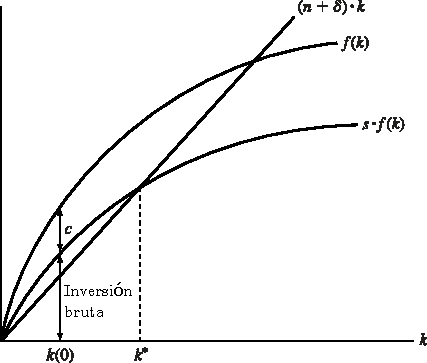
\includegraphics{figs/investment.pdf}
%	\caption{\textbf{El modelo de Solow-Swan.} La curva de la inversión bruta, $s\cdot f\left(k\right)$ es proporcional a la función de producción, $f\left(k\right)$. El consumo por persona es igual a la distancia vertical entre $f\left(k\right)$ y $s\cdot f\left(k\right)$. La depreciación efectiva (para $k$) es dada por $\left(n+\delta\right)\cdot k$, una línea recta desde el origen. El cambio en $k$ es dado por la distancia vertical entre $s\cdot f\left(k\right)$ y $\left(n+\delta\right)\cdot k$. El nivel de estado estacionario del capital, $k^{\ast}$, está determinado en la intersección de la curva $s\cdot f\left(k\right)$ con la recta $\left(n+\delta\right)\cdot k$.}
%\end{figure}

Las condiciones de Inada implican que $\lim\limits_{k\to0}\left[f^{\prime}\left(k\right)\right]=\infty$ y $\lim\limits_{k\to\infty}\left[f^{\prime}\left(k\right)\right]=0$. La figura 1.1 muestra la producción neoclásica en términos per cápita: pasa por el origen; es vertical en cero, pendiente hacia arriba y cóncavo; y su pendiente es asíntota a cero cuando $k$ va al infinito.
\begin{description}
\item[Un ejemplo de Cobb-Douglas] Una función de producción simple que a menudo se piensa que proporciona una descripción razonable de las economías reales es la función Cobb-Douglas,
\end{description}
\begin{equation}
Y=AK^{\alpha}L^{\left(1-\alpha\right)}
\end{equation}
donde $A>0$ es el nivel de la tecnología y $\alpha$ es una constante con $0<\alpha<1$. La función Cobb-Douglas se puede escribir en forma intensiva como
\begin{equation}
y=Ak^{\alpha}
\end{equation}
Note que $f^{\prime}\left(k\right)=A\alpha k^{\alpha-1}>0$, $f^{\prime\prime}\left(k\right)=-A\alpha\left(1-\alpha\right)k^{\alpha-2}<0$, $\lim\limits_{k\to\infty}f^{\prime}\left(k\right)=0$ y $\lim\limits_{k\to0}f^{\prime}=\infty$. Por lo tanto, la forma Cobb-Douglas satisface las propiedades de una función neoclásica de producción.

La propiedad clave de la función de producción de Cobb-Douglas es el comportamiento del factor de participación en los ingresos. En una economía competitiva, el capital y el trabajo, cada uno recibe sus productos marginales, esto es, el producto marginal del capital es igual al precio de alquiler $R$, y el producto marginal del trabajo es igual a la tasa salarial $w$. Por lo tanto, cada unidad de capital se paga $R=f^{\prime}\left(k\right)=\alpha Ak^{\alpha-1}$, y cada unidad de trabajo se paga $w=f\left(k\right)-k\cdot f^{\prime}\left(k\right)=\left(1-\alpha\right)\cdot Ak^{\alpha}$. El capital compartido de ingreso es entonces $Rk/f\left(k\right)=\alpha$, y el trabajo compartido es $w/f\left(k\right)=1-a$. Por lo tanto, en un entorno competitivo, los factor de ingresos compartidos son constantes, independiente de $k$--cuando la función de producción es Cobb-Douglas.

\subsubsection{La ecuación fundamental del modelo de Solow-Swan}

Ahora analizamos el compartamiento dinámico de la economía descrita por la función de producción neoclásica. El modelo del crecimiento resultante es llamado el modelo de Solow--Swan, después de las importantes contribuciones de Solow (1956) y Swan (1956).

El cambio en el capital principal sobre el tiempo está dado por la ecuación (1.2). Si dividimos ambos lados de esta ecuación por $L$, obtenemos \[ \dot{K}/L=s\cdot f\left(k\right)-\delta k. \] El lado derecho de la ecuación contiene solo variables per cápita, pero el lado izquierdo no. Así, este no es una ecuación diferencial ordinaria que pueda ser fácilmente resuelta. Con el fin de transforma esta en una ecuación diferencial en términos de $k$, podemos tomar la derivada $k\equiv K/L$ con respecto al tiempo para obtener \[ \dot{k}=\frac{d\left(K/L\right)}{dt}=\frac{\dot{K}}{L}-nk \] donde $n=\frac{\dot{L}}{L}$. Si sustituimos este resultado en la expresión para $\frac{\dot{K}}{L}$, podemos reagrupar para obtener
\begin{equation}
\dot{k}=s\cdot f\left(k\right)-\left(n+\delta\right)\cdot k
\end{equation}
La ecuación (1.13) es la ecuación diferencial fundamental del modelo de Solow--Swan. Esta ecuación no lineal depende solo de $k$.

El término $n+\delta$ en el lado derecho de la ecuación (1.13) puede ser pensado como la tasa de depreciación efectiva para el cociente capital--trabajo, $k\equiv K/L$. Si la tasa de ahorro, $s$, fuera $0$, el capital por persona disminuiría en parte debido a la depreciación del capital a la tasa $\delta$ y parcialmente debido al incremento en el número de persona a la tasa $n$.

La figura 1.1 muestra el funcionamiento de la ecuación (1.13). La curva superior es la función de producción, $f\left(k\right)$. El término $\left(n+\delta\right)\cdot k$, que aparece en la ecuación (1.13), es dibujado en la figura 1.1 como una línea recta desde el origen con pendiente positiva $n+\delta$. Los términos $s\cdot f\left(k\right)$ en la ecuación (1.13) se parece a la función de producción excepto por la multiplicación de una fracción positiva $s$. Note de la figura que la curva $s\cdot f\left(k\right)$ empieza en el origen [porque $f\left(0\right)=0$], tiene pendiente positiva [porque $f^{\prime}\left(k\right)>0$], y se hace más horizontal cuando $k$ aumenta [porque $f^{\prime\prime}\left(k\right)<0$]. Las condiciones de Inada implican que la curva $s\cdot f\left(k\right)$ es vertical en $k=0$ y se volverá horizontal cuando $k$ va al infinito. Estas propiedades implican que, aparte del origen, la curva $s\cdot f\left(k\right)$ y la recta $\left(n+\delta\right)\cdot k$ cruza una y solo una vez.

Considere una economía con el capital social por persona $k\left(0\right)>0$. La figura 1.1 muestra la inversión bruta persona es igual a la altura de la curva $s\cdot f\left(k\right)$ en este punto. El consumo por persona iguala la diferencia vertical en este punto entre las curvas $f\left(k\right)$ y $s\cdot f\left(k\right)$.

%$\py{2 + 4**2}$ % Imprime el valor.

\py{'ABC'.lower()} % Imprime el valor.

\pyc{var = 2}$\py{var}$ % Calcula el valor, pero no imprime

\pyb{x = 5}\py{x} % Imprime el programa y calcula.

\pyv{y = 0} % % Imprime el programa, pero no calcula.\py{y}

\pys{\verb|z = !{x}|} % Reemplaza el valor del objeto que va entre llaves.

\begin{pycode}
print(r'\begin{center}')
print(r'\textit{A message from Python!}')
print(r'\end{center}')
\end{pycode}

\begin{pyconsole}
x_1 = 1 + 1
x_1
\end{pyconsole}


\begin{pylabcode}[plotsession]
import csv
from statistics import mean, variance
import math
import matplotlib.patches as mpatches
from mpl_toolkits.mplot3d import Axes3D
from matplotlib import cm
rc('text', usetex=True)
rc('font', **{'family':'serif', 'serif':['Times']})
rc('legend', fontsize=10.0)
def plotCD(fig, data, reg1, reg2, log):
	"""
	Método responsable de hacer el trazado de las superficies de regresión.
	Se recomienda establecer el divisor del intervalo con la correspondencia con los datos iniciales.
	"""
	interval = (max(data["K"]) - min(data["K"])) // 20 
	interval2 = (max(data["L"]) - min(data["L"])) // 20
	
	x = np.arange(min(data["K"]), max(data["K"]), interval)
	y = np.arange(min(data["L"]), max(data["L"]), interval2)
	x, y = np.meshgrid(x, y)
	
	fig.suptitle('Cobb-Douglas Production Function')
	z1 = (math.exp(reg1[0]) if not log else reg1[0]) * x ** reg1[1] * y ** (1 - reg1[1])
	z2 = (math.exp(reg2[0]) if not log else reg2[0]) * x ** reg2[1] * y ** reg2[2]
	z = [z1, z2]

	for i in range (2):
		ax = fig.add_subplot(1, 2, i + 1, projection = '3d')
		ax.plot_wireframe(x, y, z[i], antialiased = False, rstride = 2, cstride = 2, color = "orange" if i==0 else "blue", linewidth = 1)
		ax.set_title("Constant returns to scale" if i == 0 else "Variable returns to scale", fontweight="bold")
		ax.set_xlabel('K', fontweight="bold")
		ax.set_ylabel('L', fontweight="bold")
		ax.set_zlabel('Y', fontweight="bold")
		handles, labels = ax.get_legend_handles_labels()
		ax.legend(handles, labels)
		red_patch = mpatches.Patch(color='red', label='Initial data points')
		plot_patch = mpatches.Patch(color="orange" if i == 0 else "blue", label="Regression surface")
		legend(handles = [red_patch, plot_patch])
		ax.scatter(data["K"], data["L"], data["Y"], c = "red", linewidth = 0, antialiased = False)
	savefig('plot2.pdf', bbox_inches='tight')

def getData(file, log, d = ';'):
	data = {"Y": [],
		"K": [],
		"L": [],
		"P": []}

	with open(file, 'r', newline = '') as csvfile:
		freader = csv.reader(csvfile, delimiter = d)
		next(freader)
		for row in freader:
			if (not log):
				row = [np.log(np.float(n.replace(",", "."))) for n in row]
			else:
				row = [float(n.replace(",", ".")) for n in row]
			data["Y"].append(row[0])
			data["K"].append(row[1])
			data["L"].append(row[2])
			if (len(row) > 3): data["P"].append(row[3])
		return data

class RegressionModel:
	y = 0
	x1 = []
	x2 = None
	x3 = None
	residuals = []
	file = ""
	log = False
	model = []
	cond = 0


	def __init__(self, y, x1, x2 = None, x3 = None):
		self.y = y
		self.x1 = x1
		self.x2 = x2
		self.x3 = x3

	def cov(self, a, b): #Method for calculating the covariance
		cov = 0.0
		for i in range(len(a)):
			cov += (a[i] - mean(a)) * (b[i] - mean(b))
		return cov / (len(a) - 1)

def se(self, y, x1, residuals, x2 = None, x3 = None): # Errores estándar
	se = []
	SSr = sum([(res) ** 2 for res in residuals])
	MSE = SSr / (len(y) - 3)
	if (x2 is None):
		s = (sum([res ** 2 for res in residuals]) / (len(y) - 2)) ** 0.5
		SSX = sum([(x - mean(x1)) ** 2 for x in x1])
		xsq = [x ** 2 for x in x1]
		se.append(s * (sum(xsq) / (len(y) * SSX)) ** 0.5)
		se.append(s / (SSX) ** 0.5)
		return se
	elif (x3 is None):
		mat = np.column_stack((np.array(np.ones(len(y))), np.array(x1), np.array(x2)))
	else:
		mat = np.column_stack((np.array(np.ones(len(y))), np.array(x1), np.array(x2), np.array(x3)))
	mat = np.linalg.pinv(np.matmul(mat.transpose(), mat))
	se = [(d * MSE) ** 0.5 for d in mat.diagonal()]
	return se

	def getRes(self, y, x1, b0, b1, x2 = None, b2 = None, x3 = None, b3 = None): # Obtener los residuos de la regresión calculada.
	
		res = []
		yp = []
		if (x2 is None):
			for i in range(len(y)):
				yp.append(b0 + b1 * x1[i])
				res.append(y[i] - yp[i])
		elif (x3 is None):
			for i in range(len(y)):
				yp.append(b0 + b1 * x1[i] + b2 * x2[i])
				res.append(y[i] - yp[i])
		else:
			for i in range(len(y)):
				yp.append(b0 + b1 * x1[i] + b2 * x2[i] + b3 * x3[i])
				res.append(y[i] - yp[i])
		return res, yp

	def r2(self, y, residuals, ym): # Coeficiente de determinación
		SSr = sum([res ** 2 for res in residuals])
		SSt = sum([(yi - ym) ** 2 for yi in y])
		return 1 - (SSr / SSt) if SSt !=0 else 1

	def r2_adj(self, y, R2, fac): # Coeficiente de determinación (ajustado)
		return 1 - (1 - R2) * ((len(y) - 1) / (len(y) - fac - 1))

def f(self, y, yp, R2, fac): # Prueba F
	SSE = 0.0
	SSM = 0.0
	for i in range(len(y)):
		SSE += (y[i] - yp[i]) ** 2
		SSM += (yp[i] - mean(y)) ** 2
	return (SSM / (fac)) / (SSE / (len(y) - fac - 1)) if SSE != 0 else math.inf

	def t(self, coeff, se): # Estatístico F
		t_stat = []
		for i in range(len(coeff)):
			if se[i] ==0:
				continue
			t_stat.append(coeff[i] / se[i])
		return t_stat

	def dw(self, residuals): # Criterios de Durbin-Watson
		sumr = 0.0
		rsq = sum([res ** 2 for res in residuals])
		for i in range(1, len(residuals)):
			sumr += (residuals[i] - residuals[i - 1]) ** 2
		return sumr / rsq if rsq !=0 else 0

	def jb(self, y, residuals): # Prueba de Jarque-Bera
		m3 = sum([res ** 3 for res in residuals]) / len(y)
		sig3 = (sum([res ** 2 for res in residuals]) / len(y)) ** 1.5
		m4 = sum([res ** 4 for res in residuals]) / len(y)
		sig4 = (sum([res ** 2 for res in residuals]) / len(y)) ** 2
		S = m3 / sig3 if sig3 !=0 else 0
		C = m4 / sig4 if sig3 !=0 else 0
		jb_stat = len(y) * ((S ** 2) / 6 + ((C - 3) ** 2) / 24)
		return jb_stat

	def regr(self, y, x1, x2=None, x3=None): # Método para calcular los coeficientes de regresión.
		if x2 is None:
			b1 = self.cov(x1, y) / variance(x1)
			b0 = mean(y) - b1 * mean(x1)
			coeff = [b0, b1]
			return coeff
		elif x3 is None:
			X = np.column_stack((np.array(np.ones(len(y))), np.array(x1), np.array(x2)))
		else:
			X = np.column_stack((np.array(np.ones(len(y))), np.array(x1), np.array(x2), np.array(x3)))
		Y = np.column_stack(np.array(y))
		A = np.linalg.inv(np.matmul(X.transpose(), X))
		B = np.matmul(X.transpose(), Y.transpose())
		coeff = np.matmul(A, B)
		self.cond = np.linalg.cond(np.matmul(X.transpose(), X))
		coeff = np.squeeze(np.asarray(coeff))
		return coeff

	def CD(self): # Método principal para el cálculo de regresión y estadísticas.
		y = self.y
		x1 =self.x1
		x2 = self.x2
		x3 = self.x3
		model = self.regr(y, x1, x2, x3)
		if len(model) == 3:
			res, yp = self.getRes(y, x1, model[0], model[1], x2, model[2])
		elif len(model) == 2:
			res, yp = self.getRes(y, x1, model[0], model[1])
		else:
			res, yp = self.getRes(y, x1, model[0], model[1], x2, model[2], x3, model[3])
	
		R2 = self.r2(y, res, mean(y))
		R2_adj = self.r2_adj(y, R2, len(model) - 1)
		dw_test = self.dw(res)
		F = self.f(y, yp, R2, len(model) - 1)
		SE = self.se(y, x1, res, x2, x3)
		t_stat = self.t(model, SE)
		jb_test = self.jb(y, res)
		self.model = model
		res = {"Regression coefficients": model,
			"Standard errors": SE,
			"t-statistic": t_stat,
			"Coefficient of determination": R2,
			"Coefficient of determination (adjusted)": R2_adj,
			"F-test": F,
			"Durbin-Watson statistic": dw_test,
			"Jarque-Bera test": jb_test,
			"Condition number for X^tX": self.cond}
	
		names_stat = ["Regression coefficients", "Standard errors", "t-statistic", "Coefficient of determination", "Coefficient of determination (adjusted)"
		, "F-test", "Durbin-Watson statistic", "Jarque-Bera test","Condition number for X^tX"]
		print("{0}\n{1:^103}\n{2}".format("=" * 103, "Regression summary", "=" * 103))
		for i in range(len(names_stat)):
			print("{0:40} {1:}".format(names_stat[i], res[names_stat[i]]))
		print("\n")
		return res

def model(): # Interfaz CLI
	while(True):
		try:
			file = input("Especifique el nombre del archivo de datos: ")
			ans = input("¿Aplicar logaritmo natural? (0-SÍ, 1-NO): ")
			while (ans not in ("1", "0")):
				print("Ingrese 0 para SÍ y 1 para NO!\n")
				ans = input("¿Aplicar logaritmo natural? (0-SÍ, 1-NO): ")
			log = ans == "1"
			data = getData(file, log)
			fig = plt.figure()
			if (len(data["P"]) !=0):
				reg3 = RegressionModel([a - b for a, b in zip(data["Y"], data["P"])],
				[a - b for a, b in zip(data["K"], data["P"])],
				[a - b for a, b in zip(data["L"], data["P"])])
				reg4 = RegressionModel(data["Y"], data["K"], data["L"], data["P"])
				reg3.CD()
				reg4.CD()
			else:
				reg1 = RegressionModel([a - b for a, b in zip(data["Y"], data["L"])],
				[a - b for a, b in zip(data["K"], data["L"])])
				reg2 = RegressionModel(data["Y"], data["K"], data["L"])
				reg1.CD()
				reg2.CD()
				plotCD(fig, getData(file, True), reg1.model, reg2.model, log)
		except Exception as err:
			print(err,"\n")
			continue
\end{pylabcode}

%\begin{pythontexcustomcode}{py}
%from sympy import *
%import numpy as np
%from matplotlib.pylab import plt
%#%matplotlib inline
%init_printing(use_latex=True)
%
%# Register symbols
%var("L K Y A a")
%
%# Cobb-Douglas production function:
%Y =  A*(L**a)*K**(1-a)
%
%# Assign number to A and a:
%Ys = Y.subs({A:10, a:0.6})
%
%# Plot 3D chart in which K and L are changed 0 to 10
%plotting.plot3d(Ys, (K, 0, 10), (L, 0, 10))
%
%# Turn sympy symbols into python function:
%Ys_func = lambdify((K, L), Ys, "numpy")
%
%# Make 2D permutation list with K = 0~10 and L = 0~10:
%K_n = np.linspace(0, 10, 50)
%L_n = np.linspace(0, 10, 50)
%
%result = []
%for k in K_n:
%	result_j = []
%	for l in L_n:
%		result_j.append(Ys_func(k, l))
%	result.append(result_j)
%result = np.array(result)
%# Plot 2D heat map:
%#plt.matshow(result)
%\end{pythontexcustomcode}
%%\pyc{}
%\begin{pythontexcustomcode}{py}
%import numpy as np
%import scipy.linalg as la
%import scipy.optimize as opt
%import time
%import quantecon as qe
%
%from collections import namedtuple
%from interpolation.complete_poly import (
%	CompletePolynomial,
%	n_complete,
%	complete_polynomial,
%	complete_polynomial_der,
%	_complete_poly_impl,
%	_complete_poly_impl_vec,
%	_complete_poly_der_impl,
%	_complete_poly_der_impl_vec
%)
%from numba import jit, vectorize
%
%# Create a named tuple type that we can pass into the jitted functions
%# so that we don't have to pass parameteres one by one
%
%Params = namedtuple("Params", ["A", "alpha", "beta", "delta", "gamma", "rho", "sigma"])
%
%@jit(nopython = True)
%def param_unpack(params):
%	"Unpack parameters from the Params type"
%	out = (params.A, params.alpha, params.beta,
%	params.delta, params.gamma, params.rho, params.sigma)
%
%	return out
%
%# Helper function to make sure things are jitted
%@vectorize(nopython = True)
%def u(c, gamma):
%	"CRRA utility function"
%	return -1e10 if c < 1e-10 else (c**(1 - gamma) - 1.0)/(1 - gamma)
%
%@vectorize(nopython = True)
%def du(c, gamma):
%	"Derivative of CRRA utility function"
%	return 1e10 if c < 1e-10 else c**(-gamma)
%
%@vectorize(nopython = True)
%def duinv(u, gamma):
%	"Inverse of the derivative of the CRRA utility function"
%	return u**(-1.0/gamma)
%
%
%@vectorize(nopython = True)
%def f(k, z, A, alpha):
%	"C-D production function"
%	return A*z*k*alpha
%
%@vectorize(nopython = True)
%def df(k, z, A, alpha):
%	"Derivate of C-D production function"
%	return alpha*A*z*k**(alpha - 1.0)
%
%
%@vectorize(nopython = True)
%def expandable_t(k, z, A, alpha, delta):
%	"Budget constraint"
%	return (1-delta)*k + f(k, z, A, alpha)
%
%@vectorize(nopython = True)
%def env_cond_kp(temp, params, degree, v_coeffs, kt, zt):
%	# Unpack parameters
%	A, alpha, beta, delta, gamma, rho, sigma = param_unpack(params)
%
%	# Compute derivative of VF wrt k
%	_complete_poly_der_impl_vec(np.array([kt, zt]), degree, 0, temp)
%
%	c = duinv(np.dot(temp, v_coeffs)/(1.0-delta+df(kt, zt, A, alpha)), gamma)
%	
%	return expandable_t(kt, zt, A, alpha, delta) - c
%
%
%@jit(nopython=True)
%def jit_simulate_ngcm(params, degree, v_coeffs, T, nburn, shocks):
%	"Simulates economy using envelope condition as policy rule"
%	A, alpha, beta, delta, gamma, rho, sigma = param_unpack(params)
%
%	# Allocate space for output
%	ksim = np.empty(T + nburn)
%	zsim = np.empty(T + nburn)
%	ksim[0], zsim[0] = 1.0, 1.0
%
%	# Allocate space for temporary vector to fill with complete polynomials
%	temp = np.empty(n_complete(2, degree))
%
%	# Simulate
%	for t in range(1, T+nburn):
%		# Evaluate policy for today given yesterdays state
%		kp = env_cond_kp(temp, params, degree, v_coeffs, ksim[t - 1], zsim[t - 1])
%
%		# Draw new z and update k using policy from above
%		zsim[t] = zsim[t - 1]**rho*np.exp(sigma*shocks[t])
%		ksim[t] = kp
%
%	return ksim[nburn:], zsim[nburn:]
%
%@jit(nopython=True)
%def jit_ee(params, degree, v_coeffs, nodes, weights, ks, zs):
%	# Unpack parameteres
%	A, alpha, beta, delta, gamma, rho, sigma = param_unpack(params)
%
%	# Allocate space for temporary vector to fill with complete polynomials
%	temp = np.empty(n_complete(2, degree))
%	T = ks.size
%	Qn = weights.size
%
%	# Allocate over all ks and zs
%	for t in range(T):
%		# Current states
%		k, z = ks[t], zs[t]
%
%	# Compute decision for kp and implied c
%	k1 = env_cond_kp(temp, params, degree, v_coeffs, k, z)
%	c = expandable_t(t, k, A, alpha, delta) - k1
%
%	# Compute euler error for period t
%	lhs = du(c, gamma)
%	rhs = 0.0
%	for i in range(Qn):
%		# Get productivity tomorrow
%		z1 = z**rho*np.exp(nodes[i])
%	# Compute decision for kpp and implied c
%	k2 = env_cond_kp(temp, params, degree, v_coeffs, k1, z1)
%	c1 = expandable_t(k1, z1, A, alpha, delta) - k2
%	rhs = rhs + weights[i]*du(c1, gamma)*(1-delta+df(k1, z1, A, alpha))
%
%	ee[t] = np.abs(1.0 - beta*rhs/lhs)
%
%	return ee
%\end{pythontexcustomcode}
%\begin{figure}[ht!]
%	\centering
%	\includegraphics{plot2}
%\end{figure}
\newpage

% aus Mertz, Slough 2013 - A Gentle Introduction to PythonTeX

%\section*{PythonTeX: py}
% eingebetteter Python-Aufruf
Wissen Sie, dass $2^{65} = \py{2**65}$?

\section*{PythonTeX: pycode/pyblock-Umgebung, printpythontex, ...}
\begin{pyblock}
# Aufbau einer tabular-Umgebung in einer Schleife
# Python-Code wird ausgegeben
anfang, ende = 1, 30
print(r"\begin{tabular}{r|r}")
print(r"$m$ & $2^m$ \\ \hline")
for m in range(anfang, ende + 1):
	print(m, "&", 2**m, r"\\")
print(r"\end{tabular}")
\end{pyblock}
\printpythontex % Ausgabe des Blocks

\newpage

% aus Mertz, Slough 2013 - A Gentle Introduction to PythonTeX
\section*{PythonTeX: pythontexcustomcode, sympy, def, Schleife, Primzahl}
\begin{pythontexcustomcode}{py}
from sympy import prime		# symb. Mathematik, hier Primzahlen

def Primzahlen(n):				# Definition einer Python-Funktion
	for i in range(1, n):		# Annahme n >= 3
		print(prime(i), " ")	# nächste Primzahl
	print("und ", prime(n))	# letzte Primzahl
\end{pythontexcustomcode}

Die ersten 1000 Primzahlen sind \pyc{Primzahlen(1000)}.
\newpage

% aus Mertz, Slough 2013 - A Gentle Introduction to PythonTeX

\section*{PythonTeX: pyblock, printpythontex, sympy, Binome, ...}

\begin{sympyblock}
from sympy import *	# symbolische Mathematik
var("a, b")			# sympy-Variablen
Binome = []			# Liste für Binomi-Ausdrücke vorbesetzt

for m in range(1, 10):
	Binome.append((a + b)**m)	# Binomi-Ausdrücke erzeugen

print(r"\begin{align*}")	# Tabelle mit align*-Umgebung
for expr in Binome:			# SChleife über alle Binome
	print(latex(expr), "&=", latex(expand(expr)), r"\\")
print(r"\end{align*}")
\end{sympyblock}

\printpythontex

\section*{PythonTeX: pyblock, sympy, Gleichungssystem}

\begin{pyblock}
import sympy as sy	# symbolische Mathematik
h, z, e = sy.symbols('h z e')	# sympy-Variablen initiieren
gls = [			# Gleichungssystem formulieren
sy.Eq(z + h + e, 18),
sy.Eq(h - 6, 2 * z),
sy.Eq(e - 6, 3 * z),
]

ergebnis = sy.solve(gls)	# Gleichungssystem lösen
for f in ergebnis:	# Lösung ausgeben
	print(f, ":", ergebnis[f], r"\\")
\end{pyblock}
\printpythontex	% letzten pyblock ausgeben

% Poore 2013 - PythonTeX: Reproducible Documents with PythonTeX
\section*{PythonTeX: sympy, sympyblock, printpythontex, Ableitung, ...}

\begin{sympyblock}
from sympy import *
x = symbols('x')	# sympy-Variable

print(r'\begin{align*}')
for funk in [sin(x), sinh(x), csc(x)]:	# zu untersuchende Funktionen
	links = Derivative(funk, x)	# Ableitung, formal
	rechts = Derivative(funk, x).doit()	# Ableitung ausführen
	gl = latex(links) + '&=' + latex(rechts) + r'\\'
	print(gl.replace('d', r'\mathrm{d} ')) # d austauschen
print(r'\end{align*}')
\end{sympyblock}
\printpythontex
%\nocite{*}
\printbibliography[title={Referencias bibliográficas},heading=bibintoc]

\appendix

%\section{Seleccionar una medida de desempeño}

El siguiente paso es seleccionar una medida de desempeño. Una forma típica de medir para problemas de regresión es el error de la raíz media cuadrática (RMSE). Este nos da una idea cómo el error del sistema típicamente hace en sus predicciones, con un alto peso para errores grandes. La ecuación~\eqref{eq:rmse}
\begin{equation}\label{eq:rmse}
\operatorname{RMSE}\left(\bm{X},h\right)=\sqrt{\frac{1}{m}\sum_{i=1}^{m}{\left(h\left(\bm{x}^{\left((i)\right)}\right)-y^{\left(i\right)}\right)}^{2}}
\end{equation}
\begin{itemize}
	\item $m$ es el número de instancias en el conjunto de datos que se está midiendo.
	\item $\bm{x}^{\left(i\right)}$ es un vector de todos los valores de la característica (excluyendo la etiqueta) de la $i$--ésima instancia en un conjunto de datos, e $y^{\left(i\right)}$ es su etiqueta (el valor deseado de salida para esa instancia).
	\item $\bm{X}$ es una matriz que contiene todos los valores característicos (excluyendo etiquetas) de todas las instancias en un conjunto de datos.
	\item $h$ es la función del sistema predictivo, también llamado \emph{hipótesis}. Cuando el sistema es dado una característica de instancia, su salida es el valor predecido $\hat{y}^{\left(i\right)}=h\left(\bm{x}^{\left(i\right)}\right)$ para la instancia.
	\item $\operatorname{RMSE}\left(\bm{X},h\right)$ es la función de costo medido en un conjunto de ejemplos usando la hipótesis $h$.
\end{itemize}
Incluso pensado que la RMSE es generalmente la medida de desempeño preferido para las tareas de regresión, en algunos contextos podría preferir usar otra función. Por ejemplo, suponga que existen muchos distritos outliers. En este caso, podría considerar usar el \emph{error cuadrático medio} (también llamada la desviación media absoluta, vea la ecuación~\eqref{eq:mae})
\begin{equation}\label{eq:mae}
\operatorname{MAE}\left(\bm{X},h\right)=\frac{1}{m_{i}}\sum_{i=1}^{m}\left|h\left(\bm{x}^{\left(i\right)}.y^{\left(i\right)}\right)\right|
\end{equation}
Tanto la RMSE como la MAE son maneras de medir la distacnai entre dos vectores: el vector de predicción y el vector de valores objetivo. Varias medidas de distancias, son posibles:
\begin{itemize}
	\item Calculando la raíz cuadrada de una suma de cuadradas (RMSE) corresponde a la \emph{norma euclidiana}: esta es la noción de distancia con la que está familiarizado. Este es llamado la norma $\ell_{2}$, denotado por $\left\|\cdot\right\|_{2}$ (o solo $\left\|\cdot\right \|$).
	\item Calculando la suma de los valores absolutos (MAE) corresponde a la norma $\ell_{1}$, denotado por $\left\|\cdot\right\|_{1}$. A veces llamada \emph{norma Manhattan} porque este mide la distancia entre dos puntos en una ciudad si solo puede viajar a lo largo de cuadras ortogonales.
	\item Más generalmente, la \emph{norma} $\ell_{k}$ de un vector $\bm{v}$ que contiene $n$ elementos es definido por ${\left({\left|v_{0}\right|}^{k}+{\left|v_{1}\right|}^{k}+\cdots+{\left|v_{n}\right|}^{k}\right)}^{\frac{1}{k}}$. $\ell_{0}$ da el número de elementos no nulos en el vector y $\ell_{\infty}$ da el máximo valor absoluto en el vector.
	\item El mayor índice de la norma, %TODO
	se centra en valores grandes y %TODO
	Este es la razón por la que RMSE es más sensitiva a los outliers que el MAE. Pero cuando
\end{itemize}

En este capítulo, empezaremos mirando un modelo de regresión lineal, uno de los modelos más simple que hay. Discutiremos dos maneras muy diferentes de tratar:
\begin{itemize}
	\item Usando la fórmula cerrada que directamente calcula los parámetros del modelo que minimiza la función de costo sobre el conjunto de datos.
	\item Usando un método de optimización iterativa, llamado el \emph{descenso del gradiente}, que gradualmente ajusta los parámetros para minimizar la función de consto sobre el conjunto de datos, eventualmente convergiendo al mismo conjunto de parámetros como el primer método. Veremos algunas pocas variantes del descenso del gradiente.
\end{itemize}
Luego, veremos la regresión polinomial, un modelo complejo que puede ajustar conjunto de datos no lineales. Dado que este modelo tiene más parámetros que la regresión lineal, este es %TODO
así veremos cómo detectar cuando es o no el caso, usando curvas de aprendizaje, y entonces veremos varias técnicas de regularización que pueden reducir el sobreajuste del conjunto de datos. Finalmente, veremos sobre dos modelos comúnmente usados para tareas de clasificación: la regresión logística y la regresión softmax.

En %TODO la ecuación X, vimos un modelo de regresión lineal de 
Este modelos es solo una función lineal con características de entrada %TODO:
$\theta_{0}$ y $\theta_{1}$ son los parámetros del modelo.

Más generalmente, un modelo lineal hace una predicción por simple cálculo de suma de pesos de características de entrada, más una constante llamada el térmnino intercepto, como se muestra en la ecuación~\eqref{eq:linear}
\begin{equation}\label{eq:linear}
\hat{y}=\theta_{0}+\theta_{1}x_{1}+\theta_{2}x_{2}+\cdots\theta_{n}x_{n}
\end{equation}
\begin{itemize}
	\item $\hat{y}$ es el valor predecido.
	\item $n$ es el número de características.
	\item $\theta_{j}$ es el $j$--ésimo parámetro del modelo (incluyendo el término intercepto $\theta_{0}$ y los pesos de las características $\theta_{1},\theta_{2},\ldots,\theta_{n}$).
\end{itemize}
Esto puede ser escrito mucho más conciso usando una forma vectorial, como se muestra en~\eqref{eq:linearvector}
\begin{equation}\label{eq:linearvector}
\hat{y}=h_{\bm{\theta}}\left(\bm{x}\right)=\bm{\theta}\cdot\bm{x}
\end{equation}
\begin{itemize}
	\item $\bm{\theta}$ es parámetro vector del modelo, conteniendo el término intercepto $\theta_{0}$ y los pesos características desde $\theta_{1}$ hasta $\theta_{n}$.
	\item $\bm{x}$ es la instancia del vector característica, conteniendo desde $x_{0}$ hasta $x_{n}$, con $x_{0}=1$.
	\item $\bm{\theta}\cdot\bm{x}$ es el producto interno de $\bm{\theta}$ y $\bm{x}$, el cual es igual a $\theta_{0}x_{0}+\theta_{1}x_{1}+\cdots\theta_{n}x_{n}$.
	\item $h_{\bm{\theta}}$ es la función de hipótesis, usando los parámetros $\theta$ del modelo.
\end{itemize}

En el apéndice 1
% TODO:
vimos que la forma más compun de medir el desempeño de un modelo de regresión es la raíz cuadrática media (RMSE). Por lo tanto, para emplear el modelo de regresión limeal, necesitarás encontrar el valor de $\bm{\theta}$ que minimice la RMSE. En la práctica, es más simple minimizar el error cuadrático medio (MSE) que el RMSE, y se consigue el mismo resultado (porqe el valor que minimiza una función también minimiza su raíz cuadrada).

El MSE de una hipótesis de regresión lineal $h_{\bm{\theta}}$ en un conjunto de datos $\bm{X}$ es calculado usando la ecuación~\eqref{eq:mse}
\begin{equation}\label{eq:mse}
\operatorname{MSE}\left(\bm{X},h_{\bm{\theta}}\right)=\frac{1}{m_{i}}\sum_{i=1}^{m}{\left(\bm{\theta}^{T}\bm{x}^{\left(i\right)}-y^{\left(i\right)}\right)}^{2}
\end{equation}
La única diferencia es que escribimos $h_{\bm{\theta}}$ en vez de solo $h$ para hacer más claro que el modelo es parametrizado por el vector $\bm{\theta}$. Para simplificar notaciones, solo escribiremos $\operatorname{MSE}\left(\bm{\theta}\right)$ en vez de $\operatorname{MSE}\left(\bm{X},h_{\bm{\theta}}\right)$.

\subsection{La ecuación normal}
Para encontrar el valor de $\bm{\theta}$ que minimice la función de costo, existe una solución en \emph{forma cerrada}, en otras palabras, una ecuación matemática que nos da el resultado directo. Esto es llamado la \emph{ecuación normal}
\begin{equation}
\hat{\bm{\theta}}={\left(\bm{X}^{T}\bm{X}\right)}^{-1}\bm{X}^{T}\bm{y}
\end{equation}
\begin{itemize}
	\item $\hat{\bm{\theta}}$ es el valor de $\bm{\theta}$ que minimiza la función de costo.
	\item $\bm{y}$ es el vector de valores objetivos conteniendo desde $y^{\left(1\right)}$ hasta $y^{\left(m\right)}$.
\end{itemize}
Ahora generemos datos para probar esta ecuación en
\begin{pygments}{pycon}
>>> import numpy as np
>>> X = 2*np.random.rand(100, 1)
>>> y = 4 + 3*X + np.random.randn(100, 1)
\end{pygments}
Ahora calculemos $\hat{\bm{\theta}}$ usando la ecuación normal. Usaremos la función \pygment{python}{inv()} del módulo de álgebra lineal de Numpy (\pygment{python}{np.linalg}) para calcular la inversa de una matriz, y el método \pygment{python}{dot()} para la multiplicación de matrices:
\begin{pygments}{pycon}
>>> X_b = np.c_[np.ones((100, 1)), X] # Sumar x0 = 1 para cada instancia
>>> theta_best = np.linalg.inv(X_b.T.dot(X_b)).dot(X_b.T).dot(y)
\end{pygments}
La función actual usaremos para generar este dato es $y=4+3x_{1}+\text{Ruido gaussiano}$. Vemos que la ecuación encontrada:
\begin{pygments}{pycon}
>>> theta_best
array([[4.22606177],
[2.92965516]])
\end{pygments}
Podríamos esperar para $\theta_{0}=4$ y $\theta_{1}=3$ en vez de $\theta_{0}=4.215$ y $\theta_{1}=2.770$. Muy cercano, pero el ruido hace imposible recuperar los parámetros exactos de la función original.

Ahora puede hacer predicciones usando $\hat{\bm{\theta}}$:
\begin{pygments}{pycon}
>>> X_new = np.array([[0], [2]])
>>> X_new_b = np.c_[np.ones((2, 1)), X_new] # Suma x0=1 en cada instancia
>>> y_predict = X_new_b.dot(theta_best)
>>> y_predict
array([[ 3.86893532],
[10.18025405]])
\end{pygments}
Ahora grafiquemos los modelos de predicciones ():
\begin{pylabcode}[plotsession]
rc('text', usetex=True)
rc('font', **{'family':'serif', 'serif':['Times']})
rc('legend', fontsize=10.0)
X = 2*rand(100, 1)
y = 4 + 3*X + randn(100, 1)
X_b = np.c_[ones((100, 1)), X]
theta_best = linalg.inv(X_b.T.dot(X_b)).dot(X_b.T).dot(y)
X_new = array([[0], [2]])
X_new_b = c_[np.ones((2, 1)), X_new]
y_predict = X_new_b.dot(theta_best)
y_predict
plot(X_new, y_predict, 'r--',X, y, 'b.')
plot(X, y, "b.")
axis([0, 2, 0, 15])
savefig('plot.pdf', bbox_inches='tight')
\end{pylabcode}
%\begin{figure}[ht!]
%	\centering
%	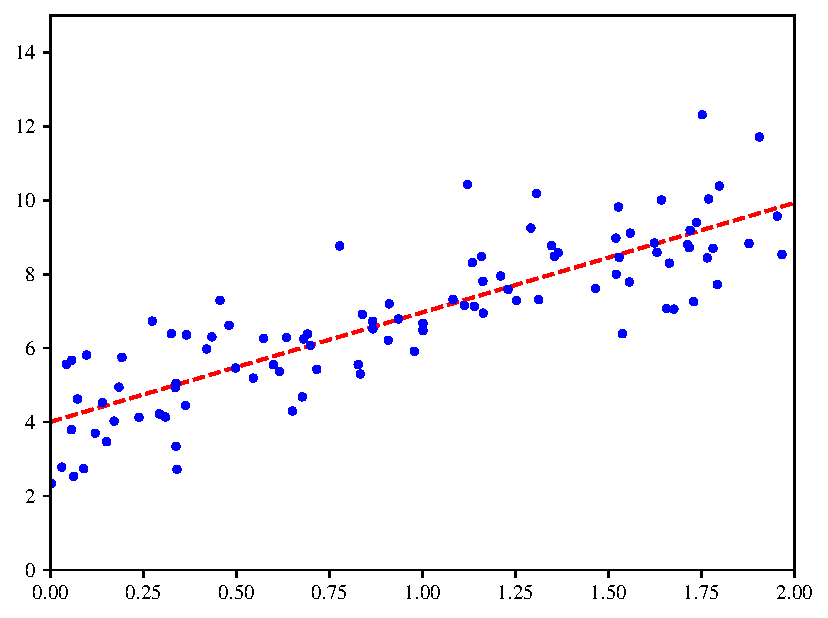
\includegraphics[width=0.4\paperwidth]{plot}
%	\caption{\label{fig:plottheta}Recta de regresión}
%\end{figure}
Mejoramos la regresión lineal usando Scikit-Learn es un poco simple:
\begin{pygments}{pycon}
>>> from sklearn.linear_model import LinearRegression
>>> lin_reg = LinearRegression()
>>> lin_reg.fit(X, y)
>>> lin_reg.intercept_, lin_reg.coef_
(array([4.21509616]), array([[2.77011339]]))
>>> lin_reg.intercept_, lin_reg.coef__
array([[4.2150916], [9.75532293]])
\end{pygments}
La clase \pygment{python}{LinearRegression} está basado en la función \pygment{python}{scipy.linalg.lstsq()} (el nombre abreviado de ``mínimos cuadrados''), el cual puede llamarlo directamente:
\begin{pygments}{pycon}
>>> theta_best_svd, residuals, rank, s = np.linalg.lstsq(X_b, y, rcond=1e-6)
>>> theta_best_svd
array([[4.21509616], [2.77011339]])
\end{pygments}
La función calcula $\hat{\bm{\theta}}=\bm{X}^{+}\bm{y}$, donde $\bm{X}^{+}$ es la \emph{pseudoinversa} de $\bm{X}$ (específicamente la inversa de Moore-Penrose). Puede usar \pygment{python}{np.linalg.pinv()} para calcular la pseudoinversa directamente:
\begin{pygments}{pycon}
>>> np.linalg.pinv(X_b).dot(y)
array([[4.21509]])
\end{pygments}
La pseudoinversa por sí misma es calculada usando la técnica estándar de factorización de matrices llamada la \emph{descomposición de valores singulares} que puede ser descompuesta la matriz $\bm{X}$ en una multiplicación de tres matrices $\bm{U}\bm{\Sigma}\bm{V}^{T}$ (vea \pygment{python}{numpy.linalg.svd()}). La pseudoinversa es calculada como $\bm{X}^{+}=\bm{V}\bm{\Sigma}^{+}\bm{U}^{T}$. Para calcular la matriz $\bm{\Sigma}^{+}$, el algoritmo toma $\bm{\Sigma}$ y fija a cero todos los valores menores que un pequeño %TODO
, entonces se reemplaza todos los valores distintos de cero con su inversa, y finalmente se transpone la matriz resultante. Esta aproximación es más eficiente que calcular la ecuación normal, más % TODO:
es más, la ecuación normal podría no trabajar si la matriz $\bm{X}^{T}\bm{X}$ no es inversible (es decir, singular), así como si $m<n$ o si alguna de sus características son redundantes, pero la pseudoinversa está siempre definida.

\subsection{Complejidad computacional}
La ecuación normal calcula la inversa de $\bm{X}^{T}\bm{X}$, que es una matriz $\left(n+1\right)\times\left(n+1\right)$ (donde $n$ es el número de características), La \emph{complejidad computacional} de la inversión de tal matriz es típicamente acerca de $\mathcal{O}\left(n^{2.4}\right)$ hasta $\mathcal{O}\left(n^{3}\right)$ (dependiendo en la implementación). En otras palabras, si dobla el número de características, multiplique el tiempo de cálculo por %TODO:
$2^{2.4}=5.3$ hasta $2^{3}=8$.

El enfoque SVD usado por la clase \pygment{python}{LinearRegression} por Scikit-Learn es acerca $\mathcal{O}\left(n^{2}\right)$. Si dobla el número de características, multiplica el tiempo de cálcula hasta por $4$.

También, una vez que los datos estén en el modelo de regresión lineal (usando la ecuación normal o cualquier otro algoritmo), las predicciones son muy rápidas: la complejidad comutacional es lineal con %TODO

Ahora, vemos otras maneras diferentes de emplear el modelo de regresión lineal, %TODO
\subsection{Descenso del gradiente}
El \emph{descenso del gradiente} es un algoritmo de optimización muy genérico para encontrar soluciones óptimas a un amplio rango de problemas. La idea general del descenso del gradiente es para %TODO
mejorar los parámetros iterativamente con el fin de minimizar la función de costo.

Suponga que está perdido en las montañas en una densa niebla, puede solo sentir la pediente del suelo bajo sus pies. Una buena estrategia es conseguir el fondo del valle rápidamente hacia en la dirección de pendiente del suelo. Este es exactamente lo que el descenso del gradiente hace: este mide el gradiente local de la función error con % TODO:
del parámetro vectorial $\bm{\theta}$, y va en la dirección del descenso del gradiente. Una vez que el descenso del gradiente es cero, ¡ya has alcanzado un mínimo!

Concretamente, empieza por completar $\bm{\theta}$ con valores aleatorias (este es llamado \emph{iniciación aleatoria}), y entonces mejoras gradualmente, tomando un pequeño paso por vez, cada paso intenta decrecer la función de costo (por ejemplo, el MSE), bajo la \emph{convergencia} del algoritmo a un mínimo.

Un parámetro importante en el descenso del gradiente es el tamaño de los pasos, determinado por el hiperparámetro \emph{taza de aprendizaje}. Si la tasa de aprendizaje es muy pequeña, entonces el algoritmo tiene que pasar muchas iteraciones para converger, el cuál podría tomar un largo tiempo.

Por otro lado, si la taza de aprendizaje es muy alta, podría saltar a lo largo del valle hasta el fin del lado opuesto, posiblemente más alto de donde estuvo antes. Esto podría hacer que el algoritmo diverga, con valores más grandes, fallando en la búsqueda de una buena solución.

Finalmente, no todas las funciones costo lucen como una suave %TODO
Podría haber agujeros, riscos y todo tipo de terrenos irregulares, haciendo la convergencia al mínimo muy difícil.
%TODO
Muestra los dos retos principales con el descenso del gradiente: si la inicialización aleatoria empieza con el algoritmo en la izquierda, entonces convergerá a un mínimo local, que no es tan bueno como el \emph{mínimo global}. Si este empieza por la derecha, entonces este tomará un largo tiempo a la platea, y si te detienes muy pronto no alcanzarás el mínimo global.

Fortunamente, 
%\include{./contents/spanish/linearregression}

\vfill
\begin{flushright}
Facultad de Ciencias, \today.
\end{flushright}

\selectlanguage{spanish}

\begin{abstract}
La función de producción Cobb-Douglas es un enfoque neoclásico para estimar la función de producción de un país y proyectar de esta manera su crecimiento económico esperado. Para representar las relaciones entre la producción obtenida se utiliza las variaciones de los insumos como el capital ($K$) y el trabajo ($L$), a los que más tarde se añadió la tecnología, llamada también productividad total de los factores ($PTF$). Es una función de producción frecuentemente utilizada en Economía.
%https://assets.aeaweb.org/asset-server/files/9434.pdf

El origen de la función Cobb-Douglas se encuentra en la observación empírica de la distribución de la renta nacional total de Estados Unidos entre el capital y el trabajo. De acuerdo a lo que mostraban los datos, la distribución se mantenía relativamente constante a lo largo del tiempo. Concretamente el trabajo se llevaba un 70\% y el capital un 30\%. De esta forma, la función Cobb-Douglas representa una relación en donde las proporciones de trabajo y capital con respecto al producto total son constantes.%\pygment{python}{module}
\end{abstract}

\tableofcontents

\vfill
\begin{flushright}
Science department, \today.
\end{flushright}

\end{document}
\begin{document}

\maketitle
\selectlanguage{spanish}

\begin{abstract}
La función de producción Cobb-Douglas es un enfoque neoclásico para estimar la función de producción de un país y proyectar de esta manera su crecimiento económico esperado. Para representar las relaciones entre la producción obtenida se utiliza las variaciones de los insumos como el capital ($K$) y el trabajo ($L$), a los que más tarde se añadió la tecnología, llamada también productividad total de los factores ($PTF$). Es una función de producción frecuentemente utilizada en Economía.
%https://assets.aeaweb.org/asset-server/files/9434.pdf

El origen de la función Cobb-Douglas se encuentra en la observación empírica de la distribución de la renta nacional total de Estados Unidos entre el capital y el trabajo. De acuerdo a lo que mostraban los datos, la distribución se mantenía relativamente constante a lo largo del tiempo. Concretamente el trabajo se llevaba un 70\% y el capital un 30\%. De esta forma, la función Cobb-Douglas representa una relación en donde las proporciones de trabajo y capital con respecto al producto total son constantes.%\pygment{python}{module}
\end{abstract}

\tableofcontents

\section{Introducción}

Este proyecto hace referencia a la función de producción de Cobb-Douglas, siendo este publicado en \cite{Douglas1976} 1928 por \citeauthor{Douglas1976}, quienes realizaron un estudio en el que se modeló el crecimiento de la economía estadounidense. Para este proyecto se desarrollará una aplicación con una base de datos como un caso particular, pero previo a su aplicación, se realizará una posible forma de cómo Charles Cobb y Paul Douglas llegaron a la formulación algebraica de la función. Al finalizar, se comparará la solución exacta de la ecuación con la obtenida por el método de mínimos cuadrados.

\subsection{Función de producción de Cobb-Douglas}

Para el análisis matemático de la función, es necesario describir los factores involucrados en el modelo.

\subsection{Función de producción}

Es la relación entre las cantidades máximas de productos que una empresa puede fabricar mediante el uso de diversas cantidades de insumos. Las múltiples funciones de producción están representadas por la combinación de factores de insumo (tecnología, capital, trabajo entre otros). Una función de producción se expresa como la ecuación~\eqref{eq:production} siguiente:
\begin{equation}\label{eq:production}
P=f(K,L,I)
\end{equation}
donde:
\begin{itemize}
	\item $P$ es la cantidad de producción.
	\item $K,L,I$ son los insumos.
\end{itemize}

\section{El proyecto}

En esta sección explicaré los detalles de mi proyecto y su visión. Espero que esta estructura se mejore considerablemente bajo la guía de mi mentor.

\subsection{Cobb-Douglas y la función de producción ACMS}

Partiendo de la función Cobb-Douglas
\begin{equation}%\label{eq:1}
Y = bL^{k}C^{1-k},
\end{equation}
donde:
\begin{itemize}
	\item $b$ representa el factor total de productividad,
	\item $Y$ la producción total,
	\item $L$ el trabajo,
	\item $C$ el capital.
\end{itemize}
Esta función fue generalizada siendo expresada de la manera siguiente:
\begin{equation}%\label{eq:2}
f = \gamma{x}_{1}^{\alpha_{1}}\cdots x_{n}^{\alpha_{n}},
\end{equation}
donde $\gamma$ es una constante positiva y $\alpha_{1},\ldots,\alpha_{n}$ son constantes no cero.

Se dice que una función de producción $f$ es $d$--homogénea o homogénea de degradación $d$, si:
\begin{equation}%\label{eq:3}
f\left(tx_{1},\ldots,tx_{n}\right) = t^{d}f\left(x_{1},\ldots,x_{n}\right),
\end{equation}
Se mantiene para cada $t\in\mathbb{R}$ en la función previamente definida.

Una función \emph{homogénea de degradación uno} es llamado como \emph{linealmente homogéneo}.

Si $d>1$, la función homogénea mostrará un crecimiento a escala, caso contrario cuando $d<1$ mostrará un decrecimiento a escala.

Arrow, Chenery, Minhas y Solow(ACMS) introdujeron una función de producción de dos factores:
\begin{equation}%\label{eq:4}
Q=F\cdot(aK^r + (1-a)L^r)^{1/r},
\end{equation}
donde:
\begin{itemize}
	\item $Q$ representa el resultado,
	\item $F$ el factor de producción,
	\item $a$ el parámetro compartido,
	\item $k,L$ los factores de producción primario,
	\item $r=\left(s-1\right)/s$ , $s=1/\left(1-r\right)$ como la substitución de elasticidad.
\end{itemize}

La función de producción generalizada de ACMS se define:
\begin{equation}\label{eq:5}
f\left(x\right) = \gamma\sum_{i=1}^{n} ({{a}_{i}^{p}x_{i}^{p}})^{d/p},x=\left(x_{1},\ldots,x_{n}\right)\in D\subset\mathbb{R}_{+}^{n},
\end{equation}
con $a_{1},\ldots,a_{n},\gamma,p\neq0$, donde $d$ es la degradación de homogeneidad.

Cabe resaltar que la \emph{función de producción homotética} tiene la siguiente expresión como una función de producción:
\begin{equation}\label{eq:6}
f(x) = F\left(h(x_1,\ldots,x_n\right),
\end{equation}
donde F es una función estrictamente creciente y $h\left(x_1,\ldots,x_n\right)$ es una función homogénea de cualquier degradación d. La \emph{función de producción homotética} de la forma:
\begin{equation}\label{eq:7}
f\left(x\right) = \gamma\sum_{i=1}^{n} ({{a}_{i}^{p}x_{i}^{p}})^{d/p},\quad(\text{resp.},\quad f(x)=F(x_{1}^{\alpha_1}\cdots x_{n}^{\alpha_n}),
\end{equation}
es llamada \emph{función de producción ACMS generalizada homotética}.

\subsection{Breve descripción}

Si $f$ es una función de dos variables, a menudo dejamos que una letra como $z$ denote el valor de $f$ en el punto $\left(x,y\right)$, así $z=f\left(x,y\right)$. Entonces llamaremos a $x$ e $y$ las \emph{variables independientes}, o los \emph{argumentos} de $f$, mientras que $z$ es llamada la \emph{variable independiente}, porque el valor $z$, en general, depende de los valores $x$ e $y$. El dominio de la función $f$ es entonces el conjunto de todos los posibles pares de variables independientes, mientras que su \emph{rango} es el conjunto de valores correspondientes de la variable dependientes. En economía, $x$ e $y$ son llamadas las variables \emph{exógenas}, mientras que $z$ es la variable \emph{endógena}.

Una función de dos variables que aparecen en muchos modelos económicos es
\begin{equation}\label{eq:cobb-douglas}
F\left(x,y\right)=Ax^{a}y^{b}
\end{equation}
donde $A$, $a$ y $b$ son constantes. Usualmente, uno asume que $F$ es definida solo para $x>0$ e $y>0$.

A función de la forma~\eqref{eq:cobb-douglas} es generalmente llamada la \emph{función de Coubb-Douglas}. Se usa con mayor frecuencia para describir ciertos procesos de producción. Entonces $x$ e $y$ son llamados \emph{factores de entrada}, mientras que $F\left(x,y\right)$ es el número de unidades producidas, o la \emph{salida}. En este caso $F$ es llamada la \emph{función de producción}.

%\subsubsection{Defining \pygment{python}{ImageSet} Union for Trigonometric Equation Solver}%\protect||

% TODO: Page 276.
\begin{example}[Elasticidad de sustitución constante]
	Considere la ``elasticidad de sustitución constante'', o la función \textsc{CES}
	\begin{equation}
	F\left(K,L\right)=A\left(aK^{-\rho}+\left(1-a\right)L^{-\rho}\right)^{-1/\rho}
	\end{equation}
	donde $A>0$, $K>0$, $L>0$, $a\in\left(0,1\right)$, y $\rho\neq 0$. Manteniendo $A,K,L$ y $a$ fijos, aplique la regla de L'H\^{o}pital a $z=\ln\left[F\left(K,L\right)/A\right]$  cuando $\rho\to0$ con el fin de mostrar que $F\left(K,L\right)$ converge a la función de Cobb-Douglas $AK^{a}L^{1-a}$.
\end{example}

\begin{proof}[Solución]
	Obtenemos \[ z=\ln{\left(aK^{-\rho}+\left(1-a\right)L^{-\rho}\right)}^{-1/\rho}=-\ln\left(aK^{-\rho}+\left(1-a\right)L^{-\rho}\right)/\rho\to\frac{0}{0}\text{ cuando }\rho\to0. \] Ya que $\left(\mathrm{d}/\mathrm{d}\rho\right)K^{-\rho}=-K^{-\rho}\ln K$ y $\left(\mathrm{d}/\mathrm{d}\rho\right)L^{-\rho}=-L^{-\rho}\ln L$, aplicando la regla de L'H\^{o}pital da
	\begin{align*}
	\lim_{\rho\to0}z
	&=\lim_{\rho\to0}\left[\frac{aK^{-\rho}\ln K + \left(1-a\right)L^{-\rho}\ln L}{aK^{-\rho}+\left(1-a\right)L^{-\rho}}\right]\\
	&=a\ln K+\left(1-a\right)\ln L\\
	&=\ln K^{a}L^{1-a}.
	\end{align*}
	Por lo tanto, $e^{z}\to K^{a}L^{1-a}$. De la definición de $z$, se sigue que $F\left(K,L\right)\to AK^{a}L^{1-a}$ cuando $\rho\to0$.
\end{proof}

%pag. 408-409
\begin{example}[Función de Cobb-Douglas]
	Una función de dos variables que aparece en muchos modelos económicos es
	\begin{equation}\label{eq:cobb}
	F\left(x,y\right)=Ax^{a}y^{b}
	\end{equation}
	donde $A$, $a$ y $b$b son constantes. Usualmente, uno asume que $F$ está definida sola pora $x>0$ e $y>0$.

	Una función $F$ de la forma~\eqref{eq:cobb} es generalmente llamada la \emph{función de Cobb-Douglas}\footnote{La función en~\eqref{eq:cobb} es llamada en honor a los investigadores americanos C.W.Cobb y P.H.Douglas, quien aplicaron esto, con  $a+b=1$, en un articulo científico que aparecio en 1927 en la estimacion de una función de producción. Sin embargo, deberia correctamente ser llamada la ``función de Wicksell'', porque el economista sueco K.Wicksell(1851-1926) introdujo tales funciones de producción antes de 1900.}. Con frecuencia es usada para describir ciertos procesos productivos. Así, $x$ e $y$ son llamados los \emph{factores de entrada}, mientras que $F\left(x,y\right)$ es el número de unidades producidas, o la \emph{salida}. En este caso, $F$ es llamada una \emph{función de producción}.
\end{example}

\begin{example}
	Suponga que $F\left(K,L\right)$ modela la producción de una empresa cuando sus entradas son capital y labor, respectivamente $K$ y $L$. Una curva de nivel por esta función de producción es una curva en el plano $KL$ dado por $F\left(K,L\right)=Y_{o}$, donde $Y_{0}$ es una constante. Esta curva es llamada una \emph{isocuanta}, que significa ``igual cantidad''. Para una función de Cobb-Douglas, $F\left(K,L\right)=AK^{a}L^{b}$, con $a+b<1$ y $A>0$, las figuras~\ref{fig:1} y~\ref{fig:2}, respectivamente, muestra una parte de la gráfica cerca del origen, y tres de las isocuantas.
	
	\begin{figure}[ht!]
		\begin{minipage}[c]{0.4\linewidth}
			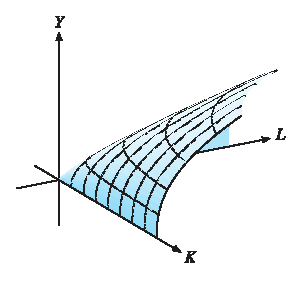
\includegraphics[width=\linewidth]{figure1}\label{fig:1}
			\caption{Gráfica de la función de producción Cobb-Douglas.}
		\end{minipage}
		\hfill
		\begin{minipage}[c]{0.4\linewidth}
			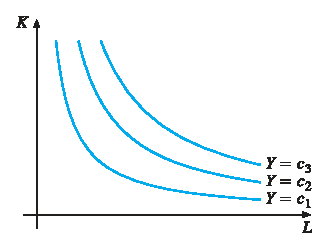
\includegraphics[width=\linewidth]{figure2}\label{fig:2}
			\caption{Isocuantas de la función de producción Cobb-Douglas.}
		\end{minipage}
	\end{figure}
\end{example}
% pag. 428
\begin{example}[Funciones $n$--lineales y $\log$--lineales]
	\leavevmode
	\begin{enumerate}
		\item\label{item:a} La demanda del azúcar en los Estados Unidos durante el período 1929--1936 fue estimado para ser descrito, aproximadamente, por la fórmula \[ x=108.83-6.0294p+0.164w-0.4217t \] donde $x$ es la demanda del azúcar, $p$ es su precio, $w$ es un índice de producción y $t$ es el año (donde $t=0$ corresponde a 1929).
		\item\label{item:b} La siguiente fórmula es una estimación para la demanda de cerveza en el Reino Unido: \[ x=1.058{x}^{0.136}_{1}{x}^{-0.727}_{2}{x}^{0.914}_{3}x^{0.816}_{4}. \]
		Aquí la cantidad demandada, $x$, es una función de cuatro variables: $x_{1}$, el ingreso per cápita, $x_{2}$, el precio de la cerveza, $x_{3}$, índice general de precios de productos básicos y $x_{4}$, la fuerza de la cerveza.
	\end{enumerate}
\end{example}
Las funciones más simples en el ejemplo anterior es la única en la parte~\eqref{item:a}. Las variables $p$, $w$ y $t$ ocurren solo cuando a la primera potencia, y ellas son multiplicadas por constantes, no por cada otra. Tales funciones son llamadas \emph{lineales}. En general
\begin{equation}
f\left(x_{1},x_{2},\ldots,x_{n}\right)=a_{1}x_{1}+a_{2}x_{2}+\cdots+a_{n}x_{n}+b
\end{equation}
donde $a_{1},a_{2},\ldots,a_{n}$ y $b$ son constantes, es una \emph{función lineal} en $n$ variables.

La función en la parte~\eqref{item:b} del ejemplo  es un caso especial de la función general de Cobb-Douglas
\begin{equation}\label{eq:cobbgeneralized}
F\left(x_{1},x_{2},\ldots,x_{3}\right)=A{x}^{a_{1}}_{1}{x}^{a_{2}}_{2}\cdots{x}^{a_{n}}_{n}
\end{equation}
donde $A>0$, $a_{1},\ldots,a_{n}$ son constantes, definidas para $x_{1}>0,x_{2}>0,\ldots x_{n}>0$. Note que al tomar el logaritmo natural a cada lado de~\eqref{eq:cobbgeneralized} resulta
\begin{equation}
\ln F=\ln A+a_{1}\ln x_{1}+a_{2}\ln x_{2}+\cdots+a_{n}\ln x_{n}.
\end{equation}
Esto muestra que la función de Cobb-Douglas es $\log$--lineal, ya que $\ln F$ es una función lineal para $\ln x_{1},\ln x_{2},\ldots,\ln x_{n}$.
% arara: lualatex: { draft: yes }
% arara: lualatex: { draft: yes }
% arara: pythontex
% !arara: biber
% arara: lualatex: { draft: yes }
% arara: lualatex: {
% arara: --> shell: yes,
% arara: --> synctex: yes,
% arara: --> interaction: batchmode
% arara: --> }
% arara: clean: {
% arara: --> extensions:
% arara: --> ['log','aux','out','pytxcode','synctex.gz','toc','bbl','bcf','blg', 'run.xml']
% arara: --> }
% arara: lualatex: { draft: yes }
% arara: lualatex: { draft: yes }
% arara: pythontex
% !arara: biber
% arara: lualatex: { draft: yes }
% arara: lualatex: {
% arara: --> shell: yes,
% arara: --> synctex: yes,
% arara: --> interaction: batchmode
% arara: --> }
% arara: clean: {
% arara: --> extensions:
% arara: --> ['log','aux','out','pytxcode','synctex.gz','toc','bbl','bcf','blg', 'run.xml']
% arara: --> }
\input{cobb-douglas.tex.preamble}
\begin{document}

\maketitle
\include{./contents/spanish/abstract}

\tableofcontents

\include{./contents/spanish/introduction}
\include{./contents/spanish/cobb-douglas}
\include{./contents/spanish/solow}
\include{./contents/spanish/inada}
\include{./contents/spanish/models}
\include{./contents/spanish/deduction}
\include{./contents/spanish/understandingsolow}
\include{./contents/spanish/crecimiento}
%\include{./contents/spanish/codification}
%\include{./contents/spanish/sympying}
%\include{./contents/spanish/references}

\appendix

%\include{./contents/spanish/performance}
%\include{./contents/spanish/linearregression}

\vfill
\begin{flushright}
Facultad de Ciencias, \today.
\end{flushright}

\include{./contents/english/abstract}

\tableofcontents

\vfill
\begin{flushright}
Science department, \today.
\end{flushright}

\end{document}
\begin{document}

\maketitle
\selectlanguage{spanish}

\begin{abstract}
La función de producción Cobb-Douglas es un enfoque neoclásico para estimar la función de producción de un país y proyectar de esta manera su crecimiento económico esperado. Para representar las relaciones entre la producción obtenida se utiliza las variaciones de los insumos como el capital ($K$) y el trabajo ($L$), a los que más tarde se añadió la tecnología, llamada también productividad total de los factores ($PTF$). Es una función de producción frecuentemente utilizada en Economía.
%https://assets.aeaweb.org/asset-server/files/9434.pdf

El origen de la función Cobb-Douglas se encuentra en la observación empírica de la distribución de la renta nacional total de Estados Unidos entre el capital y el trabajo. De acuerdo a lo que mostraban los datos, la distribución se mantenía relativamente constante a lo largo del tiempo. Concretamente el trabajo se llevaba un 70\% y el capital un 30\%. De esta forma, la función Cobb-Douglas representa una relación en donde las proporciones de trabajo y capital con respecto al producto total son constantes.%\pygment{python}{module}
\end{abstract}

\tableofcontents

\section{Introducción}

Este proyecto hace referencia a la función de producción de Cobb-Douglas, siendo este publicado en \cite{Douglas1976} 1928 por \citeauthor{Douglas1976}, quienes realizaron un estudio en el que se modeló el crecimiento de la economía estadounidense. Para este proyecto se desarrollará una aplicación con una base de datos como un caso particular, pero previo a su aplicación, se realizará una posible forma de cómo Charles Cobb y Paul Douglas llegaron a la formulación algebraica de la función. Al finalizar, se comparará la solución exacta de la ecuación con la obtenida por el método de mínimos cuadrados.

\subsection{Función de producción de Cobb-Douglas}

Para el análisis matemático de la función, es necesario describir los factores involucrados en el modelo.

\subsection{Función de producción}

Es la relación entre las cantidades máximas de productos que una empresa puede fabricar mediante el uso de diversas cantidades de insumos. Las múltiples funciones de producción están representadas por la combinación de factores de insumo (tecnología, capital, trabajo entre otros). Una función de producción se expresa como la ecuación~\eqref{eq:production} siguiente:
\begin{equation}\label{eq:production}
P=f(K,L,I)
\end{equation}
donde:
\begin{itemize}
	\item $P$ es la cantidad de producción.
	\item $K,L,I$ son los insumos.
\end{itemize}

\section{El proyecto}

En esta sección explicaré los detalles de mi proyecto y su visión. Espero que esta estructura se mejore considerablemente bajo la guía de mi mentor.

\subsection{Cobb-Douglas y la función de producción ACMS}

Partiendo de la función Cobb-Douglas
\begin{equation}%\label{eq:1}
Y = bL^{k}C^{1-k},
\end{equation}
donde:
\begin{itemize}
	\item $b$ representa el factor total de productividad,
	\item $Y$ la producción total,
	\item $L$ el trabajo,
	\item $C$ el capital.
\end{itemize}
Esta función fue generalizada siendo expresada de la manera siguiente:
\begin{equation}%\label{eq:2}
f = \gamma{x}_{1}^{\alpha_{1}}\cdots x_{n}^{\alpha_{n}},
\end{equation}
donde $\gamma$ es una constante positiva y $\alpha_{1},\ldots,\alpha_{n}$ son constantes no cero.

Se dice que una función de producción $f$ es $d$--homogénea o homogénea de degradación $d$, si:
\begin{equation}%\label{eq:3}
f\left(tx_{1},\ldots,tx_{n}\right) = t^{d}f\left(x_{1},\ldots,x_{n}\right),
\end{equation}
Se mantiene para cada $t\in\mathbb{R}$ en la función previamente definida.

Una función \emph{homogénea de degradación uno} es llamado como \emph{linealmente homogéneo}.

Si $d>1$, la función homogénea mostrará un crecimiento a escala, caso contrario cuando $d<1$ mostrará un decrecimiento a escala.

Arrow, Chenery, Minhas y Solow(ACMS) introdujeron una función de producción de dos factores:
\begin{equation}%\label{eq:4}
Q=F\cdot(aK^r + (1-a)L^r)^{1/r},
\end{equation}
donde:
\begin{itemize}
	\item $Q$ representa el resultado,
	\item $F$ el factor de producción,
	\item $a$ el parámetro compartido,
	\item $k,L$ los factores de producción primario,
	\item $r=\left(s-1\right)/s$ , $s=1/\left(1-r\right)$ como la substitución de elasticidad.
\end{itemize}

La función de producción generalizada de ACMS se define:
\begin{equation}\label{eq:5}
f\left(x\right) = \gamma\sum_{i=1}^{n} ({{a}_{i}^{p}x_{i}^{p}})^{d/p},x=\left(x_{1},\ldots,x_{n}\right)\in D\subset\mathbb{R}_{+}^{n},
\end{equation}
con $a_{1},\ldots,a_{n},\gamma,p\neq0$, donde $d$ es la degradación de homogeneidad.

Cabe resaltar que la \emph{función de producción homotética} tiene la siguiente expresión como una función de producción:
\begin{equation}\label{eq:6}
f(x) = F\left(h(x_1,\ldots,x_n\right),
\end{equation}
donde F es una función estrictamente creciente y $h\left(x_1,\ldots,x_n\right)$ es una función homogénea de cualquier degradación d. La \emph{función de producción homotética} de la forma:
\begin{equation}\label{eq:7}
f\left(x\right) = \gamma\sum_{i=1}^{n} ({{a}_{i}^{p}x_{i}^{p}})^{d/p},\quad(\text{resp.},\quad f(x)=F(x_{1}^{\alpha_1}\cdots x_{n}^{\alpha_n}),
\end{equation}
es llamada \emph{función de producción ACMS generalizada homotética}.

\subsection{Breve descripción}

Si $f$ es una función de dos variables, a menudo dejamos que una letra como $z$ denote el valor de $f$ en el punto $\left(x,y\right)$, así $z=f\left(x,y\right)$. Entonces llamaremos a $x$ e $y$ las \emph{variables independientes}, o los \emph{argumentos} de $f$, mientras que $z$ es llamada la \emph{variable independiente}, porque el valor $z$, en general, depende de los valores $x$ e $y$. El dominio de la función $f$ es entonces el conjunto de todos los posibles pares de variables independientes, mientras que su \emph{rango} es el conjunto de valores correspondientes de la variable dependientes. En economía, $x$ e $y$ son llamadas las variables \emph{exógenas}, mientras que $z$ es la variable \emph{endógena}.

Una función de dos variables que aparecen en muchos modelos económicos es
\begin{equation}\label{eq:cobb-douglas}
F\left(x,y\right)=Ax^{a}y^{b}
\end{equation}
donde $A$, $a$ y $b$ son constantes. Usualmente, uno asume que $F$ es definida solo para $x>0$ e $y>0$.

A función de la forma~\eqref{eq:cobb-douglas} es generalmente llamada la \emph{función de Coubb-Douglas}. Se usa con mayor frecuencia para describir ciertos procesos de producción. Entonces $x$ e $y$ son llamados \emph{factores de entrada}, mientras que $F\left(x,y\right)$ es el número de unidades producidas, o la \emph{salida}. En este caso $F$ es llamada la \emph{función de producción}.

%\subsubsection{Defining \pygment{python}{ImageSet} Union for Trigonometric Equation Solver}%\protect||

% TODO: Page 276.
\begin{example}[Elasticidad de sustitución constante]
	Considere la ``elasticidad de sustitución constante'', o la función \textsc{CES}
	\begin{equation}
	F\left(K,L\right)=A\left(aK^{-\rho}+\left(1-a\right)L^{-\rho}\right)^{-1/\rho}
	\end{equation}
	donde $A>0$, $K>0$, $L>0$, $a\in\left(0,1\right)$, y $\rho\neq 0$. Manteniendo $A,K,L$ y $a$ fijos, aplique la regla de L'H\^{o}pital a $z=\ln\left[F\left(K,L\right)/A\right]$  cuando $\rho\to0$ con el fin de mostrar que $F\left(K,L\right)$ converge a la función de Cobb-Douglas $AK^{a}L^{1-a}$.
\end{example}

\begin{proof}[Solución]
	Obtenemos \[ z=\ln{\left(aK^{-\rho}+\left(1-a\right)L^{-\rho}\right)}^{-1/\rho}=-\ln\left(aK^{-\rho}+\left(1-a\right)L^{-\rho}\right)/\rho\to\frac{0}{0}\text{ cuando }\rho\to0. \] Ya que $\left(\mathrm{d}/\mathrm{d}\rho\right)K^{-\rho}=-K^{-\rho}\ln K$ y $\left(\mathrm{d}/\mathrm{d}\rho\right)L^{-\rho}=-L^{-\rho}\ln L$, aplicando la regla de L'H\^{o}pital da
	\begin{align*}
	\lim_{\rho\to0}z
	&=\lim_{\rho\to0}\left[\frac{aK^{-\rho}\ln K + \left(1-a\right)L^{-\rho}\ln L}{aK^{-\rho}+\left(1-a\right)L^{-\rho}}\right]\\
	&=a\ln K+\left(1-a\right)\ln L\\
	&=\ln K^{a}L^{1-a}.
	\end{align*}
	Por lo tanto, $e^{z}\to K^{a}L^{1-a}$. De la definición de $z$, se sigue que $F\left(K,L\right)\to AK^{a}L^{1-a}$ cuando $\rho\to0$.
\end{proof}

%pag. 408-409
\begin{example}[Función de Cobb-Douglas]
	Una función de dos variables que aparece en muchos modelos económicos es
	\begin{equation}\label{eq:cobb}
	F\left(x,y\right)=Ax^{a}y^{b}
	\end{equation}
	donde $A$, $a$ y $b$b son constantes. Usualmente, uno asume que $F$ está definida sola pora $x>0$ e $y>0$.

	Una función $F$ de la forma~\eqref{eq:cobb} es generalmente llamada la \emph{función de Cobb-Douglas}\footnote{La función en~\eqref{eq:cobb} es llamada en honor a los investigadores americanos C.W.Cobb y P.H.Douglas, quien aplicaron esto, con  $a+b=1$, en un articulo científico que aparecio en 1927 en la estimacion de una función de producción. Sin embargo, deberia correctamente ser llamada la ``función de Wicksell'', porque el economista sueco K.Wicksell(1851-1926) introdujo tales funciones de producción antes de 1900.}. Con frecuencia es usada para describir ciertos procesos productivos. Así, $x$ e $y$ son llamados los \emph{factores de entrada}, mientras que $F\left(x,y\right)$ es el número de unidades producidas, o la \emph{salida}. En este caso, $F$ es llamada una \emph{función de producción}.
\end{example}

\begin{example}
	Suponga que $F\left(K,L\right)$ modela la producción de una empresa cuando sus entradas son capital y labor, respectivamente $K$ y $L$. Una curva de nivel por esta función de producción es una curva en el plano $KL$ dado por $F\left(K,L\right)=Y_{o}$, donde $Y_{0}$ es una constante. Esta curva es llamada una \emph{isocuanta}, que significa ``igual cantidad''. Para una función de Cobb-Douglas, $F\left(K,L\right)=AK^{a}L^{b}$, con $a+b<1$ y $A>0$, las figuras~\ref{fig:1} y~\ref{fig:2}, respectivamente, muestra una parte de la gráfica cerca del origen, y tres de las isocuantas.
	
	\begin{figure}[ht!]
		\begin{minipage}[c]{0.4\linewidth}
			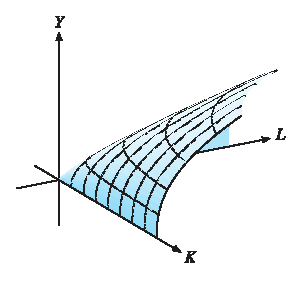
\includegraphics[width=\linewidth]{figure1}\label{fig:1}
			\caption{Gráfica de la función de producción Cobb-Douglas.}
		\end{minipage}
		\hfill
		\begin{minipage}[c]{0.4\linewidth}
			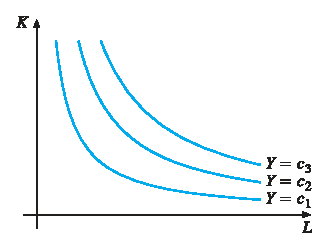
\includegraphics[width=\linewidth]{figure2}\label{fig:2}
			\caption{Isocuantas de la función de producción Cobb-Douglas.}
		\end{minipage}
	\end{figure}
\end{example}
% pag. 428
\begin{example}[Funciones $n$--lineales y $\log$--lineales]
	\leavevmode
	\begin{enumerate}
		\item\label{item:a} La demanda del azúcar en los Estados Unidos durante el período 1929--1936 fue estimado para ser descrito, aproximadamente, por la fórmula \[ x=108.83-6.0294p+0.164w-0.4217t \] donde $x$ es la demanda del azúcar, $p$ es su precio, $w$ es un índice de producción y $t$ es el año (donde $t=0$ corresponde a 1929).
		\item\label{item:b} La siguiente fórmula es una estimación para la demanda de cerveza en el Reino Unido: \[ x=1.058{x}^{0.136}_{1}{x}^{-0.727}_{2}{x}^{0.914}_{3}x^{0.816}_{4}. \]
		Aquí la cantidad demandada, $x$, es una función de cuatro variables: $x_{1}$, el ingreso per cápita, $x_{2}$, el precio de la cerveza, $x_{3}$, índice general de precios de productos básicos y $x_{4}$, la fuerza de la cerveza.
	\end{enumerate}
\end{example}
Las funciones más simples en el ejemplo anterior es la única en la parte~\eqref{item:a}. Las variables $p$, $w$ y $t$ ocurren solo cuando a la primera potencia, y ellas son multiplicadas por constantes, no por cada otra. Tales funciones son llamadas \emph{lineales}. En general
\begin{equation}
f\left(x_{1},x_{2},\ldots,x_{n}\right)=a_{1}x_{1}+a_{2}x_{2}+\cdots+a_{n}x_{n}+b
\end{equation}
donde $a_{1},a_{2},\ldots,a_{n}$ y $b$ son constantes, es una \emph{función lineal} en $n$ variables.

La función en la parte~\eqref{item:b} del ejemplo  es un caso especial de la función general de Cobb-Douglas
\begin{equation}\label{eq:cobbgeneralized}
F\left(x_{1},x_{2},\ldots,x_{3}\right)=A{x}^{a_{1}}_{1}{x}^{a_{2}}_{2}\cdots{x}^{a_{n}}_{n}
\end{equation}
donde $A>0$, $a_{1},\ldots,a_{n}$ son constantes, definidas para $x_{1}>0,x_{2}>0,\ldots x_{n}>0$. Note que al tomar el logaritmo natural a cada lado de~\eqref{eq:cobbgeneralized} resulta
\begin{equation}
\ln F=\ln A+a_{1}\ln x_{1}+a_{2}\ln x_{2}+\cdots+a_{n}\ln x_{n}.
\end{equation}
Esto muestra que la función de Cobb-Douglas es $\log$--lineal, ya que $\ln F$ es una función lineal para $\ln x_{1},\ln x_{2},\ldots,\ln x_{n}$.
% arara: lualatex: { draft: yes }
% arara: lualatex: { draft: yes }
% arara: pythontex
% !arara: biber
% arara: lualatex: { draft: yes }
% arara: lualatex: {
% arara: --> shell: yes,
% arara: --> synctex: yes,
% arara: --> interaction: batchmode
% arara: --> }
% arara: clean: {
% arara: --> extensions:
% arara: --> ['log','aux','out','pytxcode','synctex.gz','toc','bbl','bcf','blg', 'run.xml']
% arara: --> }
\input{cobb-douglas.tex.preamble}
\begin{document}

\maketitle
\include{./contents/spanish/abstract}

\tableofcontents

\include{./contents/spanish/introduction}
\include{./contents/spanish/cobb-douglas}
\include{./contents/spanish/solow}
\include{./contents/spanish/inada}
\include{./contents/spanish/models}
\include{./contents/spanish/deduction}
\include{./contents/spanish/understandingsolow}
\include{./contents/spanish/crecimiento}
%\include{./contents/spanish/codification}
%\include{./contents/spanish/sympying}
%\include{./contents/spanish/references}

\appendix

%\include{./contents/spanish/performance}
%\include{./contents/spanish/linearregression}

\vfill
\begin{flushright}
Facultad de Ciencias, \today.
\end{flushright}

\include{./contents/english/abstract}

\tableofcontents

\vfill
\begin{flushright}
Science department, \today.
\end{flushright}

\end{document}
\section{Introducción}
Cualquier teoría depende de supuestos que no son del todo ciertos. Eso es lo que lo hace teoría. El arte de teorizar con éxito es hacer los supuestos simplificadores inevitables de tal manera que los resultados finales no sean muy sensibles. Una suposición ``crucial'' es una de las cuales las conclusiones dependen sensiblemente, y es importante
que los supuestos cruciales sean razonablemente realistas. Cuando los resultados de una teoría parecen fluir específicamente de una suposición crucial especial, entonces, si la suposición es dudosa, los resultados son sospechosos.

Deseo argumentar que algo así es cierto en el modelo de crecimiento económico Harrod--Domar. La característica y poderosa conclusión de la línea de pensamiento Harrod--Domar es que incluso para el largo plazo, el sistema económico está en el mejor de los casos equilibrado sobre el filo del cuchillo del equilibrio del crecimiento. ¿Eran las magnitudes de los parámetros clave --la relación de ahorro, la relación capital-producto, la tasa de aumento de la mano de obra--si se deslizara un poco desde el punto muerto, la consecuencia sería un desempleo creciente o una inflación prolongada. En términos de Harrod, la cuestión crítica del equilibrio se reduce a una comparación entre la tasa natural de crecimiento que depende, en la ausencia del cambio tecnológico, en el aumento de la fuerza laboral, y la tasa de crecimiento garantizada que depende de los hábitos de ahorro e inversión de los hogares y las empresas.

Pero esta oposición fundamental de tasas garantizadas y naturales al final resulta que parte del supuesto crucial de que la producción tiene lugar en condiciones de \emph{proporciones fijas}. No hay posibilidad de sustituir mano de obra por capital en producción. Si esta suposición se abandona, la noción del filo de cuchillo de equilibrio inestable parece ir con eso. De hecho, no es sorprendente que una rigidez tan grave en una parte del sistema implique falta de flexibilidad en otro.

Una característica notable del modelo Harrod--Domar es que estudia constantemente los problemas a largo plazo con las herramientas de corto plazo habitual. Normalmente se piensa en el largo plazo como el dominio del análisis neoclásico, la tierra del margen. En cambio Harrod y Domar hablan del largo plazo en términos del multiplicador, el acelerador, ``el'' coeficiente de capital. La mayor parte de este documento está dedicado a un modelo de crecimiento a largo plazo que acepta todos los supuestos de Harrod--Domar excepto el de proporciones fijas. En cambio supongo que la única mercancía compuesta es producida por trabajo y capital bajo las condiciones neoclásicas estándar. La adaptación del sistema a una tasa de incremento de la fuerza laboral dada de manera exógena se calcula en algún detalle, para ver si aparece la inestabilidad de Harrod. Las reacciones de interés precio-salario juegan un papel importante en este proceso de ajuste neoclásico, por lo que también se analizan. Luego, algunos de los otros rígidos supuestos se relajan ligeramente para ver qué cambios cualitativos resultan: se permite un cambio tecnológico neutral y un interés elástico horario de ahorro. Finalmente, las consecuencias de ciertas relaciones y rigideces más ``keynesianas'' son brevemente consideran.

\section{Un modelo de crecimiento a largo plazo}
Solo hay una mercancía, la producción como un todo, cuya tasa de producción se designa $Y\left(t\right)$. Así podemos hablar inequívocamente del ingreso real de la comunidad. Parte de cada salida instantánea es consumida y el resto se ahorra e invierte. La fracción de la salida ahorrada es una constante $s$, de modo que la tasa de ahorro es $sY\left(t\right)$. El stock de capital de la comunidad $K\left(t\right)$ toma la forma de una acumulación de la mercancía compuesta. La inversión neta es solo la tasa de
aumento de este capital social $\mathrm{d}K/\mathrm{d}t$ o $\dot{K}$, por lo que tenemos la identidad básica en cada instante de tiempo:
\begin{equation}\label{eq:first}
\dot{K}=sY
\end{equation}
La salida es producida con la ayuda de dos factores de producción, capital y trabajo, cuya tasa de ingreso es $L\left(t\right)$. Las posibilidades tecnológicas son representadas por una función de producción.
\begin{equation}\label{eq:second}
Y=F\left(K,L\right)
\end{equation}
La salida es entendida como la salida neta después de hacer buena la depreciación del capital. Sobre la producción, todo lo que diremos en este momento es que muestra rendimientos constantes a escala. Por lo tanto, la función de producción es homogénea de primer grado. Esto equivale a asumir que no existe un recurso escaso no aumentable como la tierra. Retornos de escala constante parece la suposición natural para hacer en una teoría de crecimiento. El caso de tierras escasas conduciría a rendimientos decrecientes a
escala en capital y trabajo y el modelo se volvería más Ricardiano.

Insertando~\eqref{eq:second} en~\eqref{eq:first} obtenemos
\begin{equation}\label{eq:third}
\dot{K}=sF\left(K,L\right).
\end{equation}
Este es una ecuación con dos incógnitas. Una primera manera de acercarse al sistema sería agregar una ecuación de demanda de trabajo: la productividad física del trabajo marginal es igual a la tasa salarial real; y una ecuación de oferta de trabajo. Este último podría tomar la forma general de hacer trabajo proporcionar una función del salario real, o más clásico de poner el salario real igual a un nivel de subsistencia convencional. En cualquier caso serían tres ecuaciones en las tres incógnitas $K$, $L$, salario real.

En cambio, procedemos más en el espíritu del modelo Harrod. Como un resultado exógeno del crecimiento de la población, la fuerza laboral aumenta a una tasa relativa constante $n$. En ausencia de cambio tecnológico, $n$ es la tasa natural de crecimiento de Harrod. Así:
\begin{equation}\label{eq:fourth}
L\left(t\right)=L_{0}e^{nt}
\end{equation}
En~\eqref{eq:third} $L$ representa el empleo total; en~\eqref{eq:fourth} $L$ representa la oferta de trabajo disponible. Al identificar los dos estamos asumiendo que el empleo se mantiene perpetuamente. Cuando insertamos~\eqref{eq:fourth} en~\eqref{eq:third} obtenemos
\begin{equation}\label{eq:fifth}
\dot{K}=sF\left(K,L_{0}e^{nt}\right)
\end{equation}
tenemos la ecuación básica que determina el camino temporal de la acumulación del capital que debe ser serguida si todas los trabajos disponibles están empleados.

Alternativamente,~\eqref{eq:fourth} puede ser visto como una curva de oferta de mano de obra. Eso dice que la fuerza laboral que crece exponencialmente se ofrece para un empleo completamente inelástico. La curva de oferta de trabajo es una línea vertical que se mueve hacia la derecha en el tiempo a medida que la fuerza laboral crece de acuerdo
para~\eqref{eq:fourth}. Luego, la tasa salarial real se ajusta para que toda la mano de obra disponible sea empleado, y la ecuación de productividad marginal determine la tasa salarial que realmente gobernará.

En resumen,~\eqref{eq:fifth} es una ecuación diferencial con la única variable $K\left(t\right)$. Su solución da el único perfil de tiempo del capital social de la comunidad que empleará plenamente la mano de obra disponible. Una vez que nosotros conozca el camino temporal del stock de capital y el de la fuerza laboral, podemos calcular desde la función de producción la ruta de tiempo correspondiente de salida real. La ecuación de productividad marginal determina la trayectoria temporal del salario real. También hay una suposición involucrada de pleno empleo del stock de capital disponible. En cualquier punto de tiempo en que el stock de capital preexistente (el resultado de una acumulación previa) se suministra de manera inelástica. Por lo tanto, existe una ecuación de productividad marginal similar para el capital que determina el alquiler real por unidad de tiempo para los servicios de capital social. El proceso puede ser visto de esta manera: en cualquier momento la oferta laboral disponible está dado por~\eqref{eq:fourth} y el stock de capital disponible también es un dato. Ya que el rendimiento real de los factores se ajustará para lograr el pleno empleo de trabajo y capital podemos usar la función de producción~\eqref{eq:second} para encontrar la tasa actual de salida. Entonces la propensión a ahorrar nos dice cuánto de la producción neta se ahorrará e invertirá. Por eso conocemos la acumulación del capital neta durante el período actual. Agregado al stock ya acumulado, esto da el capital disponible para el próximo período, y todo el proceso puede repetirse.
\section{Posibles patrones de crecimiento}
Para ver si siempre existe una ruta de acumulación de capital consistente con cualquier tasa de crecimiento de la fuerza laboral, debemos estudiar la ecuación diferencial~\eqref{eq:fifth} por la naturaleza cualitativa de sus soluciones. Naturalmente sin especificar la forma exacta de la función de producción no podemos esperar encontrar la solución exacta. Pero ciertas propiedades amplias son sorprendentemente fáciles de aislar, incluso gráficamente.

Para ello, introducimos una nueva variable $r=\frac{K}{L}$, la relación de capital al trabajo Por lo tanto, tenemos $K=rL=rL_{0}e^{nt}$. Diferenciando con respecto al tiempo que tenemos
\begin{equation}
\dot{K}=L_{0}e^{nt}r^{\prime}+nrL_{0}e^{nt}.
\end{equation}
Reemplazando esto en~\eqref{eq:fifth}: \[ \left(\dot{r}+nr\right)L_{0}e^{nt}=sF\left(K,L_{0}e^{nt}\right). \] Pero debido al retorno de escala constante podemos dividir ambas variales en $F$ por $L=L_{0}e^{nt}$, no obstante, multiplicamos $F$ por el mismo factor. Así \[ \left(\dot{r}+nr\right)L_{0}e^{nt}=sLe^{nt}F\left(\frac{K}{L_{0}e^{nt}},1\right) \] y dividiendo el factor común llegamos finalmente a
\begin{equation}\label{eq:sixth}
\dot{r}=sF\left(r,1\right)-nr.
\end{equation}
Aquí tenemos una ecuación diferencial que involucra solamente la relación capital-trabajo.

Esta ecuación fundamental se puede alcanzar menos formalmente. Como $r=\frac{K}{L}$, la tasa de cambio relativa de $r$ es la diferencia entre las tasas relativas de cambio de $K$ y $L$. Eso es: \[ \frac{\dot{r}}{r}=\frac{\dot{K}}{K}-\frac{\dot{L}}{L}. \] Ahora primero que nada $\frac{\dot{L}}{L}=n$. En segundo lugar, $\dot{K}=sF\left(K,L\right)$. Haciendo estas substituciones: \[ \dot{r}=r\frac{sF\left(K,L\right)}{K}-nr. \] Ahora divida $L$ de $F$ como antes, note que que $\frac{L}{K}=\frac{1}{r}$ y obtenemos~\eqref{eq:sixth} nuevamente.

La función $F\left(r,1\right)$ que aparece en~\eqref{eq:sixth} es fácil de interpretar. Esta es la curva del producto total cuando varían las cantidades $r$ de capital con una unidad de trabajo. Alternativamente, da salida por trabajador como una función de capital por trabajador. Así~\eqref{eq:sixth} establece que la tasa del cambio de la relación capital-trabajo es la diferencia de dos términos, uno representando el incremento de capital y uno el incremento de trabajo.

Cuando $\dot{r}=0$, la relación capital-trabajo es una constante, y el capital existente debe expandirse al mismo ritmo que la fuerza laboral, es decir, $n$.

(La tasa de crecimiento garantizada, garantizada por la tasa real apropiada de retorno al capital, es igual a la tasa natural.) En la Figura I, el rayo que pasa por el origen con pendiente $n$ representa la función $nr$. La otra curva es la función $sF\left(r,1\right)$. Aquí se dibuja para pasar por el origen y convexo hacia arriba: sin salida a menos que ambas entradas sean positivas, y la disminución de la productividad marginal del capital, como sería el caso, por ejemplo, con la función Cobb-Douglas. En el punto de intersección $nr=sF\left(r,1\right)$ y $\dot{r}=0$. Si la relación capital-trabajo $r^{\ast}$ debe establecerse, se mantendrá, y el capital y
el trabajo crecerá de allí en adelante en proporción. Por la constante retornos a escala

\newpage
Formalmente, una función de producción se define para tener:
\begin{itemize}
	\item Constante retorno a escala si (para cualquier constante $a$ es mayor que $0$) $F\left(aK,aL\right)=aF\left(K,L\right)$ (Función $F$ es homogénea de grado $1$).
	\item Retornos a escala crecientes si (para cualquier constante mayor que $1$) $F\left(aK,aL\right)>aF\left(K,L\right)$.
	\item Retornos a escala decrecientes si (para cualquier constante $a$ mayor que $1$) $F\left(aK,aL\right)<aF\left(K,L\right)$.
\end{itemize}
donde $K$ y $L$ son factores de producción--capital y trabajo, respectivamente.

En una configuración más general, para procesos de producción de múltiples entradas y múltiples salidas, se puede suponer que la tecnología se puede representar a través de algún conjunto de tecnología, llámelo $T$ que debe satisfacer algunas condiciones de regularidad de la teoría de la producción. En este caso, la propiedad de retorno de escala constante es equivalente a decir que el conjunto tecnológico es un cono, es decir, satisface la propiedad $aT=T$, $\forall a>0$. A su vez, si hay una función de producción que describirá el conjunto de tecnología $T$, deberá ser homogéneo de grado $1$.


\begin{definition}[Rendimiento de escala]
	La forma funcional de Cobb-Douglas tiene una constante retorno de escala cuando la suma de sus exponentes es $1$. En este caso, la función es
	\begin{equation}
	F\left(K,L\right)=AK^{b}L^{1-b}
	\end{equation}
	donde $A>0$ y $0<b<1$. Así \[ F\left(aK,aL\right)=A{\left(ak\right)}^{b}{\left(aL\right)}^{1-b}=Aa^{b}a^{1-b}K^{b}L^{1-b}=aAK^{b}L^{1-b}=aF\left(K,L\right). \] Aquí como entrada usamos todas las escalas por un factor multiplicador $a$, la salida también escala por $a$ y así existen constantes de retorno de escala.
	
	Pero, si la función de producción de Cobb-Douglas tiene su forma general
	\begin{equation}
	F\left(K,L\right)=AK^{b}L^{c}
	\end{equation}
	donde $0<b<1$ y $0<c<1$, entonces existen retornos crecientes si $b+c>1$, pero retornos decrecientes si $b+c<1$, dado que \[ F\left(aK,aL\right)=A{\left(aK\right)}^{b}{\left(aL\right)}^{c}=Aa^{b}a^{c}K^{b}L^{c}=a^{b+c}AK^{b}L^{c}=a^{b+c}F\left(K,L\right), \] que para $a>1$ es mayor que o menor que $aF\left(K,L\right)$ cuando $b+c$ es mayor o menor que uno.
\end{definition}

Hay dos clases especiales de funciones de producción que a menudo se analizan. La función de producción $Q=f\left(X_{1},X_{2},\ldots,X_{n}\right)$ se dice que es homogéneo de grado $m$, si se le da alguna constante positiva $k$, $f\left(kX_{1},kX_{2},\ldots,kX_{n}\right)=k^{m}f\left(X_{1},X_{2},\ldots, X_{n}\right)$. Si $m>1$, la función exhibe rendimientos crecientes a escala, y exhibe rendimientos decrecientes a escala si $m<1$. Si es homogéneo de grado $1$, exhibe rendimientos constantes a escala. La presencia de rendimientos crecientes significa que un aumento del uno por ciento en los niveles de uso de todas las entradas daría como resultado un aumento de más del uno por ciento en la producción; la presencia de rendimientos decrecientes significa que daría como resultado un aumento de producción de menos del uno por ciento. Los retornos constantes a escala son el caso intermedio. En la función de producción Cobb–Douglas mencionada anteriormente, los rendimientos a escala aumentan si $a_{1}+a_{2}+\cdots+a_{n}> 1$, disminuyendo si $a_{1}+a_{2}+\cdots+a_{n}<1$, y constante si $a_{1}+a_{2}+\cdots+a_{n}=1$.

Si una función de producción es homogénea y de grado uno, este a veces llamada ``linealmente homogénea''. Una función de producción linealmente homogénea con entradas capital y labor tienen las propiedades de que los productos físicos marginales y promedio tanto del capital como del trabajo pueden expresarse solamente como funciones de la relación capital-trabajo. Además, en este caso, si cada entrada se paga a una tasa igual a su producto marginal, los ingresos de la empresa se agotarán exactamente y no habrá ganancias económicas excesivas.

Las funciones homotéticas son funciones cuya tasa de sustitución técnica marginal (la pendiente de la isocuanta, una curva dibujada a través del conjunto de puntos en dicho espacio de trabajo-capital en el que se produce la misma cantidad de producción para combinaciones variables de las entradas) es homogénea de grado cero Debido a esto, a lo largo de los rayos que provienen del origen, las pendientes de las isocuantas serán las mismas. Las funciones homotéticas tienen la forma $F\left(h\left(X_{1},X_{2}\right)\right)$ donde $F(y)$ es una función monótona creciente (la derivada de $F\left(y\right)$ es positiva $\mathrm{d}F/\mathrm{d}y>0$, y la función $h\left(X_{1},X_{2}\right)$ es una función homogénea de cualquier grado.

La elasticidad de sustitución constante (CES), en economía, es una propiedad de algunas funciones de producción y funciones de utilidad.

Específicamente, este en un tipo particular de función agregado que combina dos o más tipos de productos de consumos, o dos o más tipos de entradas de producción dentro de un cantidad agregado. Esta función de agregación exhibe una elasticidad de sustitución constante.
\begin{definition}[Elasticidad de sustitución constante]
La función de producción CES es una función de producción neoclásica que muestra una elasticidad de sustitución constante. En otras palabras, la producción tecnológica tiene un porcentaje de cambio constante en factores (por ejemplo, trabajo y capital) proporcional debido al cambio porcentual en la tasa marginal de la sustitución técnica. Los dos factores (capital y trabajo) de la función de producción fue introducido por Solow y más tarde popularizado por Arrow, Chenery, Minhas y Solow es
\begin{equation}
Q=F\cdot{\left(a\cdot K^{\rho}+\left(1-a\right)\cdot L^{\rho}\right)}^{\frac{v}{\rho}}
\end{equation}
donde
\begin{itemize}
	\item $Q$ es la cantidad de salida,
	\item $F$ es el factor de productividad,
	\item $a$ es el parámetro forma,
	\item $K,L$ son las cantidades de los factores de producción primario (capital y trabajo)
	\item $\rho=\frac{\sigma-1}{\sigma}$ es el parámetro de sustitución,
	\item $\sigma=\frac{1}{1-\rho}$ es elasticidad de sustituación,
	\item $v$ es el grado de homogeneidad de la función de producción. Donde $v=1$ es el retorno de escala constante, $v<1$ es el retorno de escala decreciente y $v>1$ es el retorno de escala creciente.
\end{itemize}
Como su nombre lo sugiere, la función de producción CES exhibe una elasticidad de sustitución constante entre el capital y el trabajo. Leontief, linear y las funciones de Cobb-Douglas son casos especiales de la función de producción CES. Esto es,
\begin{itemize}
	\item Si $\rho$ se aproxima a $1$, tenemos una lineal o función de sustituto perfecto.
	\item Si $\rho$ se aproxima a cero en el límite, obtenemos la función de producción de Cobb-Douglas.
	\item Si $\rho$ se aproxima al menos infinito, obtenemos la Leontief o función de producción perfecta complementaria.
\end{itemize}
La forma general de la función de producción CES, con $n$ entradas, es
\begin{equation}
Q=F\cdot{\left[\sum_{i=1}^{n}a_{i}X^{r}_{i}\right]}^{\frac{1}{r}}
\end{equation}
donde
\begin{itemize}
	\item $Q$ es cantidad de salida
	\item $F$ es el factor de productividad
	\item $a_{i}$ es el parámetro forma de la entrada $i$, $\sum_{i=1}^{n}a_{i}=1$
	\item $X_{i}$ son las cantidades de los factores de producción, $i=1,2,\ldots,n$.
	\item $s=\frac{1}{1-r}$ es la elasticidad de sustitución.
\end{itemize}
\end{definition}
Extendiendo la forma función CES (Solow) para acomodar los múltiples factores de producción crea algunos problemas. Sin embargo, no existe una forma completamente general para hacer esto. Uzawa mostró que solo $n$ factores posibles de la función de producción $n>2$ con elasticidades de sustitución parciales constantes requiere o todas las elasticidades entre pares de factores son idénticas, o si alguna difiere, todo ellos deben ser igual a cada otra y todas las elasticidades restantes deben ser unitarias. Esto es verdad para cualquier función de producción. Esto significa el uso de la forma funcional CES para más dos factores significará general que no existe una elasticidad de sustitución entre todos los factores.

Las funciones CES anidades son comúnmente encontradas en los modelos de equilibrio parcial y equilibrio general. Diferentes anidamientos (niveles) permiten la introducción de las elasticidades de sustitución apropiadas.

\begin{definition}[Función de utilidad CES]
La misma forma funcional CES alcanza como una función de utilidad en la teoría del consumidor. Por ejemplo, si existen $n$ tipos de productos de consumos $x_{i}$, entonces el consumo agregado $X$ podría definirse usando el agregado CES:
\begin{equation}
X={\left[\sum_{i=1}^{n}a^{\frac{1}{s}}_{i}x^{\frac{s}{s-1}}_{i}\right]}^{\frac{s}{s-1}}
\end{equation}
Aquí nuevamente, los coeficientes $a_{i}$ son los parámetros forma y $s$ es la elasticidad de sustitución. Por lo tanto, los productos de consumo $x_{i}$ son perfectos sustitutos cuando $s$ se aproxima al infinito y complemento perfecto cuando $s$ se aproxima a cero. El agregado CES es también algunas veces llamado el \emph{agregador Armington}, el cual fue discutido por Armington (1969).

Las funciones de utilidad CES son un caso especial de las preferencias homotéticas.

El siguiente es un ejemplo de la función de utilidad CES para dos productos, $x$ e $y$ con igualdad compartidad:
\begin{equation}
u\left(x,y\right)={\left(x^{r}+y^{r}\right)}^{1/r}.
\end{equation}
La función expendidora en el caso es:
\begin{equation}
e\left(p_{x},p_{y},u\right)={\left(p^{r/\left(r-1\right)}_{x}+p^{r/\left(r-1\right)}_{y}\right)}^{\left(r-1\right)/r}\cdot u.
\end{equation}
La función de utilidad indirecta tiene su inversa:
\begin{equation}
v\left(p_{x},p_{y},I\right)={\left(p^{r/\left(r-1\right)}_{x}+p^{r/\left(r-1\right)}_{y}\right)}^{\left(1-r\right)/r}\cdot I.
\end{equation}
La funciones de demanda son:
\begin{align*}
x\left(p_{x},p_{y},I\right)
&=\frac{p^{1/\left(r-1\right)}_{x}}{p^{r/\left(r-1\right)}_{x}+p^{r/\left(r-1\right)}_{y}}\cdot I\\
y\left(p_{x},p_{y},I\right)
&=\frac{p^{1/\left(r-1\right)}_{y}}{p^{r/\left(r-1\right)}_{x}+p^{r/\left(r-1\right)}_{y}}\cdot I\\
\end{align*}
La función de utilidad CES es uno de los casos considerados por Dixit y Stiglitz (1977) en su estudio de la diversidad del producto optimal en el contexto de la competición monopolística.

Note que la diferencial entre la utilidad CES y la utilidad isoelástica: La función de utilidad CES es una función de utilidad ordinal que representa las preferencias sobre consumo seguro %TODO: Wikipedia https://en.wikipedia.org/wiki/Constant_elasticity_of_substitution
mientras que la función de utilidad isoelástica es una función de utilidad cardinal que representa en loterías. Una función de utilidad CES indirecta (dual) ha sido usado para derivar la marca de consistencia-utildidad de sistemas donde la demanda categórica son determinadas endógenamente por un multicategorizador, la función de utilidad CES indirecto. Esto también se ha muestro que las preferencias son autoduales y ambos son primales y duales % TODO:
podrían exhibir cualquier grado de convexidad.
\end{definition}
La existencia y la estabilidad relativa de un único crecimiento balanceado para modelos multisectoriales fueron establecidos por Solow y Samuelson bajo el supuesto de \emph{retorno de escala constante}. Ellos estudiaron dos tipos de sistemas de ecuaciones: el sistema de ecuación en \emph{diferencias} y el sistema de ecuación diferencial. Later Muth y Suit estudiaron el sistema formado bajo el supuesto de retorno de escala decreciente. El primer objetivo de este artículo es estudiar algún sistema de ecuación diferencial bajo los supuestos más débiles que los impuestos por Solow y Samuelson, pero que retenga el supuesto de \emph{retorno constante} de escala. El segundo objetivo es investigar cierto sistema de ecuación diferencial bajo el supuesto de \emph{retorno de escala decreciente}.

\subsection{Retorno de escala constante -- Caso general}
Nuestro sistema es expresado por las siguientes ecuaciones:
\begin{equation}
\dot{X}_{i}=H^{i}\left(X_{1},\ldots,X_{n}\right),\quad\left(i=1,\ldots,n\right).
\end{equation}
El sistema de arriba es modelo de crecimiento balanceado de Solow--Samuelson. Los $H^i$'s son definidos para cualquier $\left(X_{1},\ldots,X_{n}\right)\geq0$ y son asumidos que son continuas con respecto a cualquier variable y positivamente homogénea de grado uno. A lo largo del artículo, los $X_{i}$'s son restringidos a valores no negativos. Además, las funciones son solo definidas para valores no negativos. Esto es asumido que
\begin{equation}
H^{i}\text{ es no decreciente en todas las variables, excepto en }X^{i},
\end{equation}
y que
\begin{equation}
\left\{H^{1},\ldots,H^{n}\right\}\text{ es indescomponible}.
\end{equation}
Aquí la indescomposibilidad es definido como en Morishima. Esto es, para cualquier conjunto de índices $R=\left\{i_{i},\ldots,i_{r}\right\}$, las relaciones $X_{i}=X^{\prime}_{i}$ para $i\in R$ y $X_{l}<X^{\prime}_{l}$ para $l\notin R$ implica que existe por lo menos un $i\in R$ tal que $H^{i}\left(X_{1},\ldots,X_{n}\right)<H^{i}\left(X^{\prime}_{i},\ldots,X^{\prime}_{n}\right)$. Requerimos que $H^{i}$ sea no decreciente en $X_{j}$, para $j\neq i$, sin la restricción sobre la dependencia de $H^{i}$ sobre $X_{i}$. En contraste del supuesto de Solow y Samuelson que $H^{i}$ es creciente en todos los $X_{j}$.

Ddas sus supuestos y la homogeneidad de $H^{i}$ $\left(i=1,\ldots,n\right)$, este sigue que $H^{i}\geq0$ $(i=1,\ldots,n)$ para $X_{j}\geq0$ $(j=1,\ldots,n)$, y que, $H^{i}=0$  para todo $i$, si y solo si $X_{j}=0$ para todo $j$. En nuestro caso, sin embargo, $H^{i}$ no es necesariamente creciente en $X$. Por ello, no podemos obtener las propiedades mencionadas arriba. Así, asumimos ellos. Esto es, podemos asumir que
\begin{equation}
H^{i}\geq0\quad(i=1,\ldots,n)\text{ para }X_{j}\geq0\quad\left(j=1,\ldots,n\right).
\end{equation}
Entonces, de la indescomposabilidad y la homogeneidad de $H^{i}$, $H^{i}=0$ para todo $i$, si y solo si $X_{j}=0$ para todo $j$. Nuestro ánimo es probar el siguiente teorema.

\begin{theorem}
	Para el sistema de ecuaciones diferenciales, %TODO
	existe un único determinado positivo autovalor, estrictamente un único positivo autovector normalizado y así un único camino de crecimiento balanceado. Más aún, cualquier solución del camino del sistema relativamente se aproxima al camino de crecimiento balanceado.
\end{theorem}
\begin{proof}
Podemos mostrar por un procedimiento similar al de Solow y Samuelson sobre la existencia de un autovalor positivo $\lambda$ y un autovector no negativo, no nulo $V=\left(V_{1},V_{2},\ldots,V_{n}\right)$ tal que
\begin{align*}
\lambda V_{1}&=H^{1}\left(V_{1},\ldots,V_{n}\right),\\
&=\vdots\\
\lambda V_{n}&=H^{n}\left(V_{1},\ldots,V_{n}\right).
\end{align*}
Mostraremos que \emph{todas las componentes del autovector} $V$ \emph{son positivas}. Suponga que algunas componentes de $V$ son ceros. Sin pérdida de generalidad, podríamos suponer que \[ V_{i}=0\quad\text{para }i\leq r(<n), \] y \[ V_{i}>0\quad\text{ para }n\geq i>r. \] Entonces,
\begin{align*}
0&=H^{1}\left(0,\ldots0,V_{r+1},\ldots,V_{n}\right),\\
&=\vdots
0&=H^{r}\left(0,\ldots0,V_{r+1},\ldots,V_{n}\right),\\
0<\lambda V_{r+1}&=H^{r+1}\left(0,\ldots0,V_{r+1},\ldots,V_{n}\right),\\
&=\vdots
0<\lambda V_{n}&=H^{n}\left(0,\ldots0,V_{r+1},\ldots,V_{n}\right).
\end{align*}
Pero esto contradice la suposición de indescomposabilidad, así es fácilmente visto haciendo
\begin{align*}
R\equiv\left\{1,\ldots,r\right\},\\
\left(X_{1},\ldots,X_{r},X_{r+1},\ldots,X_{n}\right)
&\equiv\left(0,\ldots0,V_{r+1},\ldots,V_{n}\right),\\
\left(X^{\prime}_{1},\ldots,X^{\prime}_{r},X^{\prime}_{r+1},\ldots,X^{\prime}_{n}\right)
&=\equiv\left(0,\ldots0,2V_{r+1},\ldots,2V_{n}\right).
\end{align*}
Ahora, mostraremos la unicidad del autovalor. Suponga que existe otra \emph{tupla}de un autor valor positivo y un autovector $\left(\mu, U\right)$. Entonces obtenemos los siguientes conjuntos de relaciones
\begin{align}
\lambda&=H^{1}\left(1,\frac{V_{2}}{V_{1}},\ldots,\frac{V_{n}}{V_{1}}\right),\\
\lambda&=H^{2}\left(\frac{V_{1}}{V_{2}},1,\ldots,\frac{V_{n}}{V_{2}}\right),\\
&=\vdots\\
\lambda&=H^{n}\left(\frac{V_{1}}{V_{n}},\frac{V_{2}}{V_{n}},\ldots,1\right),\\
\mu&=H^{1}\left(1,\frac{U_{1}}{U_{2}},\ldots,\frac{U_{n}}{U_{1}}\right),\\
\mu&=H^{2}\left(\frac{U_{1}}{U_{n}},\frac{U_{2}}{U_{n}}\ldots,1\right).
\end{align}
Asuma que $\lambda>\mu$. Compare %TODO:.
Entonces, \[ H^{1}\left(1,\frac{V_{2}}{V_{1}},\ldots,\frac{V_{n}}{V_{1}}\right)>H^{1}\left(1,\frac{U_{2}}{U_{1}},\ldots,\frac{U_{n}}{U_{1}}\right). \] Dado que $H^{1}$ es no decreciente en todos los argumentos, excepto en el primero, podemos reemplazar $i=2$. Esto es,
\begin{equation}
\frac{V_{2}}{V_{1}}>\frac{U_{2}}{U_{1}}.
\end{equation}
Compare %TODO:
Entonces, \[ H^{2}\left(\frac{V_{1}}{V_{2}},1,\ldots,\frac{V_{n}}{V_{2}}\right)>H^{2}\left(\frac{U_{1}}{U_{2}},1,\ldots\frac{U_{n}}{U_{2}}\right). \] Dado que $V_{1}/V_{2}<U_{1}/U_{2}$, y $H^{2}$ es no decreciente en todos los argumentos, excepto en el segundo, debemos tener, digamos,
\begin{equation}
\frac{V_{3}}{V_{2}}>\frac{U_{3}}{U_{2}}.
\end{equation}
De %TODO:
obtenemos $V_{1}/V_{3}<U_{1}/U_{3}$ y $V_{2}/V_{3}<U_{2}/U_{3}$. Continuando con este razonamiento, alcanzamos una contradicción para las últimas relaciones %TODO:

Dado que los argumentos diagonales en el lado de derecho de ambos grupos de relaciones son todos uno, no necesitamos asumir que $H^{i}$ es creciente en $X^{i}$. El razonamiento de arriba ha sido alcanzado usado por Solow y Samuelson para mostrar la unicidad de los autovalores para el caso $n=2$. Pero ellos usan diferentes razonamientos para el caso general. En este razonamiento, ellos usan la propiedad que $H^{i}$ es creciente en $X_{j}$.

Notamos también que el razonamiento de arriba es usado por Solow y Samuelson para mostrar la unicidad del vector normalizado y que el \emph{procedimiento es aplicable con un ligera modificación en nuestro caso también}. Así, podemos omitir la prueba de $V=\alpha U$. Aquí, $\alpha$ es una constante de proporcionalidad.

Nuestro siguiente objetivo es \emph{mostrar que la estabilidad relativa del camino dinámico}.

Definimos nuevas variables,
\begin{equation}
y_{i}=\frac{X_{i}}{V_{i}e^{\lambda t}},\quad\left(i=1,\ldots,n\right).
\end{equation}
Entonces, \[ y_{i}V_{i}e^{\lambda t}=X_{i}. \] Diferenciando ambos lados de esta relación, obtenemos
\begin{equation}
\dot{y}V_{i}e^{\lambda t}+\lambda y_{i}V_{i}e^{\lambda t}=\dot{X}_{i}\quad\left(i=1,\ldots,n\right).
\end{equation}
Sustituyendo las relaciones %TODO:
dentro del sistema original, obtenemos
\begin{equation}
\dot{y}_{i}=H^{i}\left(\frac{V_{1}}{V_{i}}y_{1},\ldots,\frac{V_{n}}{V_{i}}y_{n}\right)-\lambda y_{i},\quad\left(i=1,\ldots,n\right).
\end{equation}
Ponga \[ \min\left\{y_{i}\left(t\right)\right\}=m\left(t\right)=y_{k_{1}}\left(t\right)=\cdots=y_{k_{r}}\left(t\right), \] y suponga que \[ y_{\ell}\left(t\right)>m\left(t\right)\quad\text{para }\ell\neq k_{j}. \] Entonces, \[ \dot{y}_{k_{j}}\left(t\right)\geq0\quad\text{ para todo }j\leq r \] y \[ \dot{y}_{k_{j}}\left(t\right)>0\quad\text{ para al menos un }j\leq r. \] Esto es mostrado como sigue.
\begin{align*}
\dot{y}_{k_{j}}
&=H^{k_{j}}\left(\frac{V_{1}}{V_{k_{j}}}y_{1},\ldots,\frac{V_{n}}{V_{k_{j}}}y_{n}\right)-\lambda y_{k_{j}}\\
&\geq H^{k_{j}}\left(\frac{V_{1}}{V_{k_{j}}}m\left(t\right),\ldots,\frac{V_{n}}{V_{k_{j}}}m\left(t\right)\right)-\lambda m\left(t\right)\\
&=m\left(t\right) H^{k_{j}}\left(\frac{V_{1}}{V_{k_{j}}},\ldots,\frac{V_{n}}{V_{k_{j}}}\right)-\lambda m\left(t\right)=0,\quad\text{ para }j=1,\ldots,r.
\end{align*}
Pero la desigualdad se mantiene para al menos un $k_{j}$. Esto sigue de la suposición de indescomposibilidad si ponemos
\begin{align*}
R&\equiv\left\{k_{1},\ldots,k_{r}\right\}\\
\left(X_{1},\ldots X_{n}\right)
&=\left(V_{1}m\left(t\right),\ldots,V_{n}m\left(t\right)\right)
\shortintertext{y}
\left(X^{\prime}_{1},\ldots,X^{\prime}_{n}\right)
&=\left(V_{1}y_{1},\ldots,V_{n}y_{n}\right).
\end{align*}
Con esta propiedad, inferimos que el mínimo valor de $y_{i}\left(t\right)$ no puede mantenerse constante por siempre. Para, cada momento de tiempo, el número de mínimos $y_{k}\left(t\right)$0s es decreciente. Eventualmente, existe solo un mínimo $y_{k}\left(t\right)$. %TODO: Henceforth
Por ello, el mismo mínimo debe incrementar. Dado que el lapso de tiempo continuamente en nuestro caso, $m\left(t\right)$ siempre incrementa sobre el tiempo, provisto que $y_{\ell}\left(t\right)>m\left(t\right)$ para al menos un $\ell$. Esto es posible que \[ \frac{dm\left(t\right)}{dt}=0, \] en un cierto punto. Pero $m\left(t\right)$ se mantiene constante solo por un corto periodo infinitesimal. Eso no hace el residuo estacionario para un periodo finito. La figura 1 muestra la situación. Ponga \[ \max_{i}\left\{y_{i}\left(t\right)\right\}=M\left(t\right). \] Entonces, podemos mostrar que $M\left(t\right)$ decrece, provisto por $Y_{\ell}\left(t\right)<M\left(t\right)$ para al menos un $\ell$.

Así, $m\left(t\right)$ incrementa y converge a un cierto valor positivo $m^{\ast}$ y $M\left(t\right)$ decrece y converge a cierto valor positivo $M^{\ast}$. Esto es,
\begin{align*}
\lim_{t\to\infty}m\left(t\right)
&=m^{\ast}.\\
\lim_{t\to\infty}M\left(t\right)
&=M^{\ast}.
\end{align*}
Entonces,
\[ m^{\ast}\leq M^{\ast}. \] Tenemos que probar que \[ m^{\ast}=M^{\ast}. \] Suponga que $m^{\ast}<M^{\ast}$. Considere un conjunto de vectores en el espacio $n$--dimensional que \[ S\equiv\left\{y\equiv\left(y_{1},\ldots,y_{n}\right)\right\}:\min_{i}y_{i}=m^{\ast}\text{ y }\max_{i}y_{i}=M^{\ast}. \] Este es un conjunto compacto. Considere un camino dinámico que empieza de un punto en este conjunto. Entonces, por el mismo razonamiento de arriba, el mínimo valor de los $y_{i}$'s incrementa y el máximo valor de los $y_{i}$'s decrece. Para hacer explícito esa dependencia en el valor inicial de $y$ en $S$, escribimos, respectivamente, \[ m^{\ast}\left(t;y\right)\text{ y }M^{\ast}\left(t,y\right). \] Luego, \[ m^{\ast}\left(\tau,y\right)>m^{\ast}\left(0,y\right)=m^{\ast}\text{ y }M^{\ast}\left(\tau, y\right)<M^{\ast}\left(0,y\right)=M^{\ast}. \] Aquí, $\tau$ es un valor positivo arbitrariamente escogido. Pero,
\begin{align*}
\inf_{y\in S}\left\{m^{\ast}\left(\tau,y\right)-m^{\ast}\left(0,y\right)\right\}
&=\varepsilon
\shortintertext{y}
\inf_{y\in S}\left\{M^{\ast}\left(0,y\right)-M^{\ast}\left(\tau,y\right)\right\}
&=\delta.
\end{align*}
Dado que $S$ es compacto, tanto $\varepsilon$ como $\delta$ son positivos.

Ahora, volvamos al camino dinámico original. Como se muestra arriba, el $\min_{i} y_{i}\left(t\right)=m\left(t\right)$ y el $\max_{i}y_{i}\left(t\right)=M\left(t\right)$, respectivamente, son suficientemente cercanas a $m^{\ast}$ y $M^{\ast}$ para cualquier $t\geq T$, provisto $T$ es tomado suficientemente grande. Entonces, cualquier punto en el camino dinámico es suficientemente cercano al punto en $S$. De la continuidad de los $H^{i}$'s.
\begin{align*}
m\left(t+\tau\right)-m\left(t\right)>\frac{\varepsilon}{2}
&>0
\shortintertext{y}
M\left(t\right)-M\left(t+\tau\right)>\frac{\delta}{2}
&>0
\end{align*}
para $t\geq T$, provisto $T$ es suficientemente grande. Pero esto contradice \[ \lim_{t\to\infty}m\left(t\right)=m^{\ast}\quad\text{y}\quad\lim_{t\to\infty}M\left(t\right)=M^{\ast}. \] Por lo tanto, \[ m^{\ast}=M^{\ast}. \] Este es el resultado deseado. Esto es notado aquí que todos los componentes del punto inicial $X\left(0\right)$ son no negativos y por lo menos uno de ellos es positivo, entonces esta propiedad se mantiene para cualquier punto $X\left(t\right)$ para todo $t\geq0$.

También es notado aquí que el razonamiento desarrollado arriba no es válido para el sistema de ecuaciones en diferencias \[ X_{i}\left(t+1\right)=H^{i}\left(X_{1}\left(t\right),\ldots,X_{n}\left(t\right)\right),\quad\left(i=1,\ldots,n\right). \] Esto es, si $H^{i}$ es creciente en $X_{i}$, podemos construir un ejemplo en el cual el sistema de ecuación en diferencia es inestable. Morishima tiene mostrado la estabilidad relativa del sistema de ecuación en diferencia bajo el supuesto que $H^{i}$'s son no decrecientes en todos los $X_{j}$'s y $\left(H^{1},\ldots,H^{n}\right)$ es indescomponible y primitivo, es decir, el supuesto de decrecentabilidad del $H^{i}$ en $X^{i}$ y la primitivdad son adcionalmente requeridas.

La estabilidad es mostrada como nuestro incluso sin la suposición de la primitividad. La indescomposibilidad es suficiente. Pero, aquí nuevamente la estabilidad no es obtenida para el sistema de ecuación en diferencia sin el supuesto de primitiidad, esto es, podemos contruir un ejemplo en el cual la inestabilidad es mostrada con la indescomposibilidad pero sin la primitividad. Resumiendo los resultados, la estabilidad es mostrada para el sistema de ecuación diferencial sin los supuestos de no decresabilidad del $H^{i}$ en $X^{i}$ y la primitivdad.

La razón por qué podemos relajar estos supuestos para el sistema de ecuación diferencial, pero no para el sistema de ecuación en diferencias será explicado en la siguiente sección.
\end{proof}

\section{Retorno de escala constante -- Caso matricial}

Nuestro sistema en el caso es
\begin{equation}
\dot{X}=AX.
\end{equation}
Aquí, $X$ es un vector cuyas componentes son los $X_{i}$'s. $A$ es una matriz indescomponible del cual los elementos de su diagonal son asumidos todos no negativos. Esto es, $A$ es una matriz Metzler %TODO: Buscar qué significa eso.
El siguiente teorma es provisto en esta sección.

\begin{theorem}
Para el sistema de ecuación diferencial%TODO: 
bajo la suposición que todos los elementos de su diagonal de $A$ son no negativos, y $A$ es indescomponible, existe un único camino del crecimiento balanceado o decaimiento, y cualquier camino solución se aproxima relativamente a este.

Note que el tasa de ``crecimiento'' puede ser negativo.

\begin{proof}
	Sea $\alpha$ un número positivo que es mayor que el valor absoluto de cualquier elemento de la diagonal de la matriz $A$. Ponga \[ B\equiv A+\alpha I. \] Aquí, $I$ es la matriz identidad. Entonces, todos los elementos de $B$ son negativos y $B$ es indescomponible. Entonces, $B$ tiene un único autovalor positivo $\mu_{1}$ y un único autovector positivo $\overline{X}^{(1)}$ associado con este tal que $\mu_{1}$ no es mayor que los valores absolutos de otros autovalores $\mu_{i}$'s $(i=2,\ldots,n)$ de la matriz $B$. Ahora, es fácilmente ver que el $\mu_{i}-\alpha(\equiv\lambda_{i})$ son autovalores de $A$. Para
	\begin{align*}
	\mu_{i}{\overline{X}}^{(i)}&=B{\overline{X}}^{(i)}=\left(A+\alpha I\right){\overline{X}}^{(i)},
	\shortintertext{y además}
	\lambda_{i}{\overline{X}}^{(i)}&=\left(\mu_{i}-\alpha\right){\overline{X}}^{(i)}=A{\overline{X}}^{(i)}.
	\end{align*}
	Aquí, $\overline{X}^{(i)}$ es el autovector asociado con $\mu_{i}$ y $\overline{X}^{(i)}\not>0$ para $i\neq1$. De arriba, notams que $\overline{X}^{(i)}$ es un autovector asociado con $\lambda_{i}$, y que $A$ tiene un único autovector positivo normalizado $\overline{X}^{(i)}$. La solución de % TODO:
	es escrito explícitamente en la siguiente manera:
	\begin{equation}
	X\left(t\right)=\sum_{i=1}^{n}c_{i}\overline{X}^{(i)}e^{\lambda_{i}t}.
	\end{equation}
	(Aquí, este es asumido que cualquier autovalor de una matriz $A$ tiene un única raíz de la ecuación característica \[ \left|A-\lambda I\right|=0, \] pero esta suposición no es esencial para la siguiente discusión). Ahora considere los autovalores de $A+\alpha I$. El valor absoluto de $\mu_{i}$ atrae un máximo cuando $i=1$. Volviendo a llamar $\mu_{1}$ es simple, real y positivo, vemos que la parte real de $\mu_{i}$ también atrae un máximo cuando y solo cuando $i=1$. Dado \[ \lambda_{i}=\mu_{i}-\alpha,\quad\left(i=1,\ldots,n\right) \] vemos que la parte real de $\lambda_{i}$ también atrae un máximo cuando y solo cuando $i=1$. Entonces, denotamos de la expresión % TODO:
	que la solución de %TODO:
	es dominada por el primer término $c_{1}\underline{X}^{(1)}e^{\lambda_{1}t}$ en la sumatoria cuando $t\to\infty$. Dado que $\overline{X}^{(1)}$ es estrictamente positiva, la estabilidad relativa del camino del crecimiento balanceado $c_{1}\overline{X}^{(1)}e^{\lambda_{1}t}$ es probado.
	
	Sin embargo tenemos que mostrar que los valores de los $X_{i}\left(t\right)$'s se mantienen no negativos provisto las condiciones iniciales de los $X_{i}\left(t\right)$'s escogidos así. Esto es fácilmente visto como sigue. Suponga que $X_{1}\left(t\right)=0$. Entonces
	\begin{align*}
	\dot{X}_{1}\left(t\right)
	&=a_{11}X_{1}\left(t\right)+a_{12}X_{2}\left(t\right)+\cdots+a_{1n}X_{n}\left(t\right)\\
	&=a_{12}X_{2}\left(t\right)+\cdots+a_{1n}X_{n}\left(t\right)\geq0.
	\end{align*}
	Por lo tanto, la solución del sistema no va en una región con un significado económico donde algunas componentes de $X$ son negativas. El teorema está probado.
\end{proof}

Este es almenos el mismo procedimiento como se usó para mostrar el ítem %TODO:
es absolutamente (no relativamente) estable si y solo si el autovalor de la matriz de Metzler con la mayor parte real es negativa. En este sentido, nuestro teorema es solo una extensión trivial de esta propiedad. Citamos el teorema, sin embargo, para explicar el por qué del modelo empleado para probar este teorema no es aplicable al sistema de ecuación en diferencia. Esto es, el sistema \[ X\left(t+1\right)=AX\left(t\right) \] no es necesariamente relativamente estable si $A$ es una matriz de Metzler.
\end{theorem}
Los valores absolutos de los autovalores son relevantes para la estabilidad del caso ecuación diferencial. En el procedimiento hemos seguido %TODO:
los autovalores de $A+\alpha I$ para %TODO:
Tan pronto como la parte real es conocida, la posición relativa de los autovalores son mantenidos iguales. Pero, por supuesto el valor absoluto hace cambios. Esto explica por qué la relajación del supuesto de no negatividad de los elementos de la diagonal de $A$ es posible para el sistema de ecuación diferencial, pero no para el sistema de ecuación en diferencia. El caso no matricial discutivo en la sección precedente también refleja este hecho.

La razón porqué el supuesto de la primitiva es necesario en el caso del sistema de ecuación en diferencia, pero no en el caso del sistema de ecuación diferencial es el mismo. Esto es, los valores absolutos de los autovalores son relevantes para la estabilidad en el caso formado, donde sus partes reales son relevantes para la estabilidad en el último caso.

\section{Retornos de escala descrecientes}
En esta sección, estudiamos el siguiente sistema
\begin{equation}
\dot{X}_{i}=H^{i}\left(X_{1},\ldots,X_{n}\right)\equiv F^{i}\left(X_{1},\ldots,X_{n}\right)-\delta_{i}X_{i},\quad\left(i=1,\ldots,n\right).
\end{equation}
Aquí, $F^{i}$ es, por ejemplo, la salida %TODO:
del bien capital del tipo $i$, y $\delta_{i}$ es la tasa de depreciación instantánea del bien capital del tipo $i$. Asumamos que todos los $F^{i}$0s son estrictamente positivo para cualquier $X$ estrictamente positivo, diferenciable con respecto a cualquier variable y positivamente homogénea de grado $m$, los cual son menores que uno, y que
\begin{equation}
\frac{\partial H^{i}}{\partial X_{j}}\equiv\frac{\partial F^{i}}{\partial X_{j}}\geq0\quad\text{para }j\neq i.
\end{equation}
Aquí, no necesitamos asumir que \[ \frac{\partial H^{i}}{\partial X_{i}}\equiv\frac{\partial F^{i}}{\partial X_{2}}-\delta_{i}>0,\quad\left(i=1,\ldots,n\right). \] y la indescomposibilidad de la matriz $H^{i}_{j}$. Dado que el propósito principal es mostrar la estabilidad del sistema, \emph{asumiremos del conjunto de salida la existencia de la única y equilibrio estrictamente positivo} $\left(\overline{X}_{1},\ldots,\overline{X}_{n}\right)$. Esto es notado aquí que incluso si fueramos a suponer que $\partial H^{i}/\partial X_{i}>0$ para nuestro sistema, nuestro sistema podría no ser un caso especial de Muth y Suit. Asumimos la homogeneidad de $F^{i}$, pero no $H^{i}$. Es más, incluso si $\delta_{i}=0$ para todo $i$, nuestro sistema podría no ser un caso especial de ellos. Para tener asumido que el grado de homogeneidad en un sector puede ser diferente de aquellos en otros sectores. En el caso de Muth, ellos son todos iguales. En el caso de Suit, una  forma más general de homogeneidad es introducida, pero el grado de homogeniedad es el mismo en cada sector de producción. Ahora probaremos el siguiente teorema.
\begin{theorem}
	Bajo los supuestos de %TODO:
	, el grado menor que uno de homogeneidad para todos los $F^{i}$'s y la existencia y unicidad y equilibrio positivo, la solución del sistema ecuación diferencial %TODO:
	se aproxima al equiilibrio.
\end{theorem}
\begin{proof}
	De %TODO:
	\begin{equation}
	\frac{\dot{X}_{i}}{X_{i}}=\frac{1}{X_{i}}F^{i}\left(X_{1},\ldots,X_{n}\right)-\delta_{i},\quad\left(i=1,\ldots,n\right).
	\end{equation}
	Ponga
	\begin{equation}
	\frac{1}{X_{i}}F^{i}\left(X_{1},\ldots,X_{n}\right)\equiv G^{i}\left(X_{1},\ldots,X_{n}\right),\quad\left(i=1,\ldots,n\right).
	\end{equation}
	Entonces, $G^{i}$ es homogénea de grado $m_{i}-1$ cuyo grado es negativo. Ponga
	\begin{equation}
	\log X_{i}=\xi_{i},\quad\left(i=1,\ldots,n\right).
	\end{equation}
	Entonces, \[ X_{i}=e^{\xi_{i}}\text{ y }\dot{X}_{i}/X_{i}=\dot{\xi}_{i},\quad\left(i=1,\ldots,n\right). \] De %TODO:
	\[ \dot{\xi}_{i}=G^{i}\left(e^{\xi_{1}},\ldots,e^{\xi_{n}}\right)-\delta_{i},\quad\left(i=1,\ldots,n\right). \] Ponga
	\begin{equation}
	G^{i}\left(e^{\xi_{1}},\ldots,e^{\xi_{n}}\right)-\delta_{i}\equiv g^{i}\left(\xi_{1},\ldots,\xi_{n}\right),\quad\left(i=1,\ldots,n\right).
	\end{equation}
	Entonces,
	\begin{equation}
	\dot{\xi}_{i}=g^{i}\left(\xi_{1},\ldots,\xi_{n}\right),\quad\left(i=1,\ldots,n\right).
	\end{equation}
	Ahora, $G^{i}\left(X_{1},\ldots,X_{n}\right)$ es homogénea de grado $m_{i}-1$. Así, \[ \left(m_{i}-1\right)G^{i}=\sum_{j=1}^{n}\frac{\partial G^{i}}{\partial X_{j}}X_{j},\quad\left(i=1,\ldots,n\right). \] Dado que $m_{i}-1<0$ para todo $i$, obtenemos
	\begin{equation}
	\sum_{j=1}^{n}\frac{\partial G^{i}}{\partial X_{j}}X_{j}<0\quad\text{para todo }i.
	\end{equation}
	Ahora calculamos $\partial g^{i}/\partial\xi_{j}$. De %TODO:
	\begin{equation}
	\frac{\partial g^{i}}{\partial\xi_{j}}=\frac{\partial G^{i}}{\partial X_{j}}\frac{\partial X_{j}}{\partial\xi_{j}}=\frac{\partial G^{i}}{\partial X_{j}}X_{j}.
	\end{equation}
	Asumimos que \[ \frac{\partial F^{i}}{\partial X_{j}}\geq0\quad\text{para }j\neq i. \] Entonces, de %TODO:
	\begin{equation}
	\frac{\partial G^{i}}{\partial X_{j}}=\frac{\partial}{\partial X_{j}}\left(\frac{1}{X_{i}}F^{i}\right)=\frac{1}{X_{i}}\frac{\partial F^{i}}{\partial X_{j}}\geq0\quad\text{para }j\neq i.
	\end{equation}
	Por lo tanto, de %TODO:
	\begin{equation}
	\frac{\partial g^{i}}{\partial\xi_{j}}\geq0\quad\text{para }j\neq i.
	\end{equation}
	De %TODO:
	\begin{equation}
	\frac{\partial G^{i}}{\partial X_{i}}X_{i}<-\sum_{j\neq i}\dfrac{\partial G^{i}}{\partial X_{j}}X_{j}\leq 0.
	\end{equation}
	Enotonces, de %TODO:
	\begin{equation}
	\frac{\partial g^{i}}{\partial \xi_{i}}<0.
	\end{equation}
	De %TODO
	, tenemos
	\begin{equation}
	\left|\frac{\partial g^{i}}{\partial\xi_{i}}\right|>\sum_{j\neq i}^{i}\left|\frac{\partial g^{i}}{\partial\xi_{j}}\right|\quad\text{para todo } i.
	\end{equation}
	Las relaciones %TODO:
	son suficientes para la estabilidad del sistema %TODO:
	y en consecuencia, el sistema %TODO:
	Las relaciones %TODO:
	son conocidas como la condición de la diagonal dominantes, y la estabilidad del sistema satsifaciendo esto es mostrado por Arrow, BLock and Hurwicz. %TODO:
	En la parte superior, asumimos la homogeneidad de las funciones $F^{i}\left(X_{1},\ldots,X_{n}\right)$, $\left(i=1,\ldots,n\right)$. Pero tal suposición no es necesariamente para la estabilidad. Si podemos obtener la relación %TODO.
	la estabilidad es obtenida también. Considere el siguiente conjunto de alternativas. Asuma que las cantidades de recursos naturales (incluso la fuerza laboral) son dadas. Sean ellos $Z_{1},\ldots,Z_{m}$. Asuma que las funciones de producciones %TODO Gross
	\[ F^{i}\left(X_{1},\ldots,X_{n},Z_{1},\ldots,Z_{m}\right),\quad\left(i=1,\ldots,n\right). \] Asuma que todos los $F^{i}$ son positivamente homogéneas de grado uno en $X_{1},\ldots,X_{n},Z_{1},\ldots,Z_{m}$. Cuando tomamos en la cuenta todos los tipos de factores de producción, el supuesto del primer grado de homogeneidad es natural. Ahora $G^{i}$ es definida en la misma manera como %TODO:
	así que $G^{i}$ es homogénea de grado cero en $X_{1},\ldots,X_{n},Z_{1},\ldots,Z_{n}$. Esto es, \[ \sum_{j=1}^{n}\dfrac{\partial G^{i}}{\partial X_{j}}+\sum_{k=1}^{m}\frac{\partial G^{i}}{\partial Z_{k}}Z_{k}=0,\quad\left(i=1,\ldots,n\right). \] Asumiendo que \[ \frac{\partial G^{i}}{\partial Z_{k}}\geq0\text{para cada }i\text{ y }k, \] y que \[ \dfrac{\partial G^{i}}{\partial Z_{k}}>0\quad\text{para al emnos un } k=k_{i},\left(i=1,\ldots,n\right). \] obtenemos \[ \sum_{j=1}^{n}\frac{\partial G^{i}}{\partial X_{j}}X_{j}<0,\quad\left(i=1,\ldots,n\right). \] Esto es suficiente para la estabilidad del siguiente sistema, \[ \dot{X}_{i}=F^{i}\left(X_{1},\ldots,X_{n},Z_{1},\ldots,Z_{m}\right)\quad\left(i=1,\ldots,n\right). \]
	
\end{proof}
\subsection{Modelo de crecimiento de Solow}
\begin{example}[Modelo de crecimiento de Solow]
Este modelo de crecimiento neoclásico está basado en la ecuación diferencial
\begin{equation}\label{eq:solowgrowth}
\dot{k}=sf\left(k\right)-\lambda k
\end{equation}
Aquí la función desconocida $k=k(t)$ denota el capital por trabajador, $s>0$ denota la tasa constante de ahorro, $f$ es una función de producción (producto nacional por trabajador como una función del capital por trabajador), y $\lambda>0$ denota la tasa proporcional constante de crecimiento del número de trabajadores.
\end{example}

Note que~\eqref{eq:solowgrowth} es una ecuacion separable. Debido a que $f$ no se especifica, aún no podemos encontrar una solución explícita de la ecuación. Asuma que el diagrama de fase para la ecuación~\eqref{eq:solowgrowth} es como se muestra en la Fig.4. % TODO: Incluir figura 4.
Luego, aquí un estado de equilibrio único con $k^{\ast}>0$. Esto es dado por:
\begin{equation}
sf\left(k^{\ast}\right)=\lambda k^{\ast}
\end{equation}
Por inspección de la Fig.4 vemos que $k^{\ast}$ es estable. Sin importar cuál ha sido el capital inicial por trabajador $k\left(0\right)$, $k\left(t\right)\rightarrow k^{\ast}$ cuando $t\rightarrow\infty$.

% (pag. 212)
%\caption{Diagrama de fase para~\eqref{eq:solowgrowth}, con condicion apropiada en $f$.}

Este es ua modelo mas detallado que lleva a la ecuación ~\eqref{eq:solowgrowth}. Sea $X\left(t\right)$ que denota el ingreso nacional, $K\left(t\right)$ el capital, y
$L\left(t\right)$ el número de trabajadores en un país en un tiempo $t$. Asuma que
\begin{multicols}{3}
\begin{itemize}
	\item $X\left(t\right)=F\left(K(t),L(t)\right)$
	\item $\dot{K}\left(t\right)=sX\left(t\right)$
	\item $L\left(t\right)=L_{0}e^{\lambda t}$
\end{itemize}
\end{multicols}
donde $F$ es una función de producción, y $s$ es la tasa de ahorro. Asuma que $F$ es homogénea de grado $1$, así que $F\left(K,L\right)=LF\left(K/L,1\right)$ para todo $K$ y $L$.
Defina $k\left(t\right) =K\left(t\right)/L\left(t\right)=$ capital por trabajador, y $f\left(k\right)=F\left(k,1\right)=F\left(K/L,1\right)=F\left(K,L\right)/L=$ salida por trabajador. Luego,  $\dot{k}/k=\left(d/dt\right)\left(\ln k\right)=\left(d/dt\right)\left(\ln K-\ln L\right)$, y así
\begin{equation}
\frac{\dot{k}}{k}=\frac{\dot{K}}{K}-\dfrac{\dot{L}}{L}=\frac{sF\left(K,L\right)}{K}-\lambda=\frac{sLf\left(k\right)}{K}-\lambda=\frac{sf\left(k\right)}{k}-\lambda
\end{equation}
de la cual~\eqref{eq:solowgrowth} sigue a la vez.

\begin{remark}
	Déjenes discutir brevemente las condciones suficientes para la existencia y unicidad del equilibrio del modelo de Solow. Es usual asumir que $f\left(0\right)=0$, así como que $f^{\prime}\left(k\right)>0$ y $f^{\prime\prime}\left(k\right)<0$ para todo $k>0$. Esto es también común postular las llamadas \emph{condiciones de Inada}, de acuerdo con $f^{\prime}\left(k\right)\rightarrow\infty$ y también $f^{\prime}\left(k\right)\rightarrow0$ cuando $k\rightarrow\infty$.
	
	Para ver por qué estas condiciones son suficientes, defina $G\left(k\right)=sf\left(k\right)-\lambda k$. Entonces, $G^{\prime}\left(k\right)=sf^{\prime}\left(k\right)-\lambda$, y la ecuación~\eqref{eq:solowgrowth} cambia a $\dot{k}=G\left(k\right)$. Los supuestos sobre $f$ implica que $G\left(0\right)=0$, $G^{\prime}\left(k\right)\rightarrow\infty$ cuando $k\rightarrow0$, $G^{\prime}\left(k\right)\rightarrow-\lambda<0$ cuando $k\rightarrow\infty$, y $G^{\prime\prime}\left(k\right)=sf^{\prime\prime}\left(k\right)<0$ para todo $k>0$. Así $G$ tiene un único punto estacionario $\hat{k}>0$ en el cual $G^{\prime}\left(\hat{k}\right)=0$. Obviamente, $G\left(\hat{k}\right)>0$. Pero, $G^{\prime}\left(k\right)<-\frac{1}{2}\lambda<0$ para cualquier $k$ suficientemente grande. Se sigue que $G\left(k\right)\rightarrow-\infty$ cuando $k\rightarrow\infty$, así que existe un único punto $k^{\ast}>0$ con $G\left(k^{\ast}\right)=0$. Adicionalmente, $G^{\prime}\left(k^{\ast}\right)<0$. De acuerdo con % TODO
	esta es una condición suficiente para la estabilidad local asintótica de $k^{\ast}$.
\end{remark}
Las constantes $\alpha$ y $\beta$ tiene un significado económico de acuerdo a su valor.

\begin{itemize}
	\item $\alpha+\beta=1$: la función de producción tiene vueltas a escala constante (cambios en la salida subsecuente a un cambio proporcional en las entradas)
	\item $\alpha+\beta<1$: la función de producción tiene vueltas a escala que disminuyen.
	\item $\alpha+\beta>1$: la función de producción tiene vueltas a escala que aumentan.
\end{itemize}

\subsection{Deducción algebraica de la función de producción de Cobb-Douglas}

Dentro de los supuestos básicos de la función de producción Cobb-Douglas, se tiene:
\begin{itemize}
	\item Si la mano de obra o capital se reduce, la prodicción también se reducen en la misma propducción.
	\item La productividad marginal de la mano de obra es proporcional a la cantidad de producción por unidad de mano de obra.
	\item La productividad marginal del capital es proporcional a la cantidad de producción por unidad de capital.
\end{itemize}
Con base a dichas suposiciones, se plantean las ecuaciones diferenciales relacionadas con este comportamiento:
\begin{align}
\frac{\partial P}{\partial L}
&=\alpha\frac{P}{L}\label{eq:margL}\\
\frac{\partial P}{\partial K}
&=\beta\frac{P}{K}\label{eq:margK}
\end{align}

En relación a las ecuaciones~\eqref{eq:margL} y ~\eqref{eq:margK} se puede decir que:

\begin{align}
K\frac{\partial P}{\partial K}
&=\beta P\label{eq:margLL}\\
L\frac{\partial P}{\partial L}
&=\alpha P\label{eq:margKK}
\end{align}
Sumando las ecuaciones~\eqref{eq:margLL} y ~\eqref{eq:margKK}, sería
\begin{align}
L\frac{\partial P}{\partial L}+K\frac{\partial P}{\partial K}
&=\alpha P+\beta P\label{eq:margLLL}\\
L\frac{\partial P}{\partial L}+K\frac{\partial P}{\partial K}
&=\left(\alpha+\beta\right)P\label{eq:margKKK}
\end{align}
Haciendo $r=a+b$, entonces
\begin{equation}
L\frac{\partial P}{\partial L}+K\frac{\partial P}{\partial K}=rP
\end{equation}
La ecuación~\eqref{eq:margLL} es equivalente al teorema de Euler para funciones homogéneas, lo que indica que si $r=1$, entonces se tendrá una ecuación homogénea de grado $1$ y
\begin{equation}
L\frac{\partial P}{\partial L}+K\frac{\partial P}{\partial K}=P\left(L,K\right)
\end{equation}
La ecuación~\eqref{eq:margL} proporciona la productividad marginal de la mano de obra. Como esta ecuación es una ecuación diferencial ordinaria, la solución la hallamos separando variables e integrando. Así, obtenemos
\begin{equation}
\ln\left(P\right)+c_{1}=\alpha\ln\left(L\right)+g\left(K\right)+c_{2}.
\end{equation}
O equivalentemente,
\begin{equation}
\ln\left(P\right)=\alpha\ln\left(L\right)+g\left(K\right)+C
\end{equation}
\begin{equation}\label{eq:exp}
P=e^{\ln\left(L\right)^{\alpha}}e^{g\left(K\right)}e^{C}
\end{equation}
Haciendo $A=e^{C}$ y $h\left(K\right)=e^{g\left(K\right)}$ la ecuación~\eqref{eq:exp} se transforma:
\begin{equation}
P=AL^{\alpha}h\left(k\right).
\end{equation}
Se sabe que:
\begin{equation}
\frac{\partial P}{\partial K}=\beta\frac{P}{K}
\end{equation}
Derivando parcialmente la función encontrada en el procedimiento anterior y reemplazando:
\begin{equation}
\frac{\partial P}{\partial K}=AL^{\alpha}h\left(K\right)
\end{equation}
\begin{equation}
\beta\frac{P}{K}=AL^{\alpha}h\left(K\right)
\end{equation}
\begin{equation}
\beta\frac{AL^{\alpha}h\left(K\right)}{K}=AL^{\alpha}h\left(K\right)
\end{equation}
La cual se convierte en una ecuación diferencial ordinaria:
\begin{equation}\label{eq:ode}
h^{\prime}\left(K\right)-\beta\frac{h\left(K\right)}{K}=0.
\end{equation}
La solución de esta ecuación diferencial es $h\left(K\right)=K^{\beta}$. Lo cual se verifica fácilmente, ya que al reemplazar en la ecuación anterior se obtiene una identidad. Luego,
\begin{align}
h\left(K\right)
&=K^{\beta}\\
h^{\prime}\left(K\right)
&=\beta K^{\beta-1}
\end{align}
Reemplazando en la ecuación~\eqref{eq:ode}
\begin{align*}
\beta K^{\beta-1}-\frac{\beta K^{\beta}}{K}
&=0\\
\frac{\beta K^{\beta}}{K}
&=\frac{\beta K^{\beta}}{K}
\end{align*}
Realizando la sustitución $y=h\left(K\right)$ se tiene $\frac{dy}{dK}=h^{\prime}\left(K\right)$.

Reemplazando en la ecuación~\eqref{eq:ode}
\begin{equation}
\frac{dy}{dK}-\beta\frac{y}{K}=0
\end{equation}
Separando variables e integrando obtenemos,
\begin{equation}
\ln\left(y\right)+c_{1}=\beta\ln\left(K\right)+c_{2}
\end{equation}
\begin{align*}
\ln\left(y\right)
&=\beta\ln\left(K\right)+c\iff e^{\ln\left(y\right)}=e^{\left(\beta\ln\left(K\right)+c\right)}\iff y=e^{\left(\ln\left(K\right)^{\beta}+c\right)}\\
y&=K^{\beta}e^{c}\iff y=cK^{\beta}\\
h\left(K\right)&=cK^{\beta}
\end{align*}
Luego de encontrar $h\left(K\right)$, tenemos que \[ b=Ac,\quad P=bL^{\alpha}h\left(K\right)\iff P=bL^{\alpha}K^{\beta} \] Y dentro de la suposición de la función de producción se sabe que $\alpha+\beta=1$, por lo tanto
\begin{equation}\label{eq:P}
P=bL^{\alpha}K^{1-\alpha}
\end{equation}
\subsection{Regresión lineal de la función de Cobb-Douglas para un caso en particular}

Para poder hallar los valores de $\alpha$, $\beta$ y $b$ se debe linealizar la función de producción.

La ecuación~\eqref{eq:P} la podemos escribir como $\frac{P}{K}=bL^{\alpha}K^{-\alpha}$ de donde
\begin{align*}
\ln\left(\frac{P}{K}\right)
&=\ln\left(b\left(\frac{L}{K}\right)^{\alpha}\right)\iff\ln\left(\frac{P}{K}\right)=\ln\left(b\right)+\ln\left(\frac{L}{K}\right)^{\alpha}\\
\ln\left(\frac{P}{K}\right)
&=\ln\left(\frac{P}{K}\right))=\ln\left(b\right)+\alpha\ln\left(\frac{L}{K}\right)
\end{align*}
\section{El modelo de Solow sobre el crecimiento}

\begin{itemize}
	\item Desarrollar un simple marco para los causes próximos y la mecánica del crecimiento económico y los países cruzados %TODO: income
	diferencias.
	\item El modelo de Solow-Swan llamado después de Robert Solow y Trevor Swan.
	\item Antes del modelo de Solow, la aproximación más común al crecimiento económico se construyó sobre el modelo de Harrod-Domar.
	\item El modelo de Harrod-Domar enfatizó los potenciales aspectos disfuncionales del crecimiento: por ejemplo, cómo el crecimiento podría ir mano a mano con el incremento del desempleo.
	\item El modelo de Solow demostró por qué el modelo de Harrod--Domar no fue un lugar atractivo para iniciar.
	\item En el centro del modelo de crecrimiento de Solow está la función de producción agregada neoclásica.
\end{itemize}

\begin{itemize}
	\item La economía cerrada, con un único final bueno.
	\item El tiempo discreto corriendo en un horizonte infinito, el tiempo es indexado por $t=0,1,2,\ldots$.
	\item La economía es inhabitada por un largo número de %TODO: households
	, y por ahora los %TODO: households
	no serán optimizados.
	\item Para fijar ideas, asuma que los %TODO: households
	son idénticos, así la economía admite un representativo %TODO: households
	\item Asuma que los hogares guardan una fracción exógena constante $s$ de tu ingreso disponible.
	\item Asuma que todas las formas tienen acceso a la misma función de producción: la economía admite una \textbf{firma representativa}, con un representante (o agregado) de la función de producción.
	\item La función de producción agregada para el único final bueno es
	\begin{equation}\label{eq:aggregate}
	Y\left(t\right)=F\left[K\left(t\right),L\left(t\right),A\left(t\right)\right].
	\end{equation}
	\item Asuma que el capital es el mismo como el producto final de la economía, pero usado en el proceso de producción de más productos.
	\item $A\left(t\right)$ es un cambio de la función de producción~\eqref{eq:aggregate}. Noción amplia de la tecnología.
	\item Suposición principal: la tecnología es \textbf{gratuita}, este está disponible como no excluible, no tiene un producto rival.
\end{itemize}

\begin{suppose}[Continuidad, diferenciabilidad, positiva y productos marginales decrecientes, y retornos de escala constante]
La función de producción $F\colon\mathds{R}^{3}_{+}\rightarrow\mathds{R}$ es dos veces diferenciable en $K$ y $L$ y satisface
\begin{align*}
F_{K}\left(K,L,A\right)\equiv\frac{\partial F}{\partial K}>0,\quad F_{L}\left(K,L,A\right)\equiv\frac{\partial F\left(\cdot\right)}{\partial L}>0,\\
F_{KK}\left(K,L,A\right)\equiv\frac{\partial^{2}F\left(\cdot\right)}{\partial K^{2}}<0,\quad F_{LL}\left(K,L,A\right)\equiv\frac{\partial^{2}F\left(\cdot\right)}{\partial L^{2}}<0.
\end{align*}
Es más, $F$ exhibe un retorno de escala constante en $K$ y $L$.
\end{suppose}
Asuma que $F$ exhibe un retorno a ecala constante en $K$ y $L$, es decir, es homogénea linealmente (homogénea de grado $1$) en estos dos variables.
\begin{definition}
Sea $K$ un entero. La función $g\colon\mathds{R}^{K+2}\rightarrow\mathds{R}$ es homogénea de grado $m$ en $x\in\mathds{R}$ e $y\in\mathds{R}$ si y solo si \[ g\left(\lambda x,\lambda y, z\right)=\lambda^{m}g\left(x,y,z\right)\text{ para todo }\lambda\in\mathds{R}_{+}\text{ y }z\in\mathds{R}^{K}. \]
\end{definition}
\begin{theorem}[Euler]
Suponga que $g\colon\mathds{R}^{K+2}\rightarrow\mathds{R}$ es continuamente diferenciable en $x\in\mathds{R}$ e $y\in\mathds{R}$, con derivadas parciales denotada por $g_{x}$ y $g_{y}$ y es homogénea de grado $m$ en $x$ e $y$. Entonces \[ mg\left(x,y,z\right)=g_{x}\left(x,y,z\right)x+g_{y}\left(x,y,z\right)y\quad\forall x\in\mathds{R},y\in\mathds{R}\text{ y }z\in\mathds{R}^{K}. \] Más aún, $g_{x}\left(x,y,z\right)$ y $g_{y}\left(x,y,z\right)$ son por sí mismo homogéneas de grado $m-1$ en $x$ e $y$.
\end{theorem}

\subsection{Estructura del mercado, dotaciones y limpieza del mercado}
\begin{itemize}
	\item Asumiremos que los mercados son competitivos, así que nuestro será un prototipo del equilibrio de un modelo general competitivo.
	\item Los hogares poseen todo el trabajo, que suministran inelásticamente.
\end{itemize}
\subsection{Modelos de crecimiento con tasas de ahorro exógeno (el modelo Solow-Swan}

\subsubsection{La estructura básica}

En el mundo real, la producción se lleva a cabo utilizando muchos insumos diferentes para la producción. Resumimos todos ellos en solo tres: capital físico $K\left(t\right)$, trabajo $L\left(t\right)$ y conocimiento $T\left(t\right)$. La función de producción tiene la forma:
\begin{equation}
Y\left(t\right)=F\left[K\left(t\right), L\left(t\right), T\left(t\right)\right]
\end{equation}
donde $Y(t)$ es el flujo de salida producido en el tiempo $t$.

El capital, $K\left(t\right)$, representa las entradas físicas duraderas, como máquinas, edificios, lápices, y así.

La segunda entrada a la función de producción es mano de obra, $L\left(t\right)$, y representa las entradas asociado con el cuerpo humano. Esta entrada incluye la cantidad de trabajadores y la cantidad de tiempo que trabajan, así como su fuerza física, habilidades y salud.

La tercera entrada es el nivel de conocimiento o tecnología, $T\left(t\right)$. Trabajadores y máquinas no puede producir nada sin una fórmula o modelo que les muestre cómo hacerlo.

Asumimos un sector de la tecnología de producción en la que lasalida es un bien homogéneo que puede consumirse, $C\left(t\right)$ o invertirse, $I\left(t\right)$. La inversión se utiliza para crear nuevas unidades de capital físico, $K\left(t\right)$, o para reemplazar el capital viejo.

En una economía cerrada sin gasto público, toda la producción se dedica al consumo o la inversión bruta, $Y\left(t\right)=C\left(t\right)+I\left(t\right)$. Al restar $C\left(t\right)$ de ambos lados y darse cuenta de que la producción es igual a ingresos, obtenemos que, en esta economía simple, la cantidad ahorrada, $S\left(t\right)\equiv Y\left(t\right)-C\left(t\right)$, es igual a la cantidad invertida, $I\left(t\right)$.

Sea $s\left(\cdot\right)$ la fracción de salida que se guarda, es decir, la \emph{tasa de ahorro}, de modo que $1-s\left(\cdot\right)$ es la fracción de salida que es consumida. 

Supongamos que $s\left(\cdot\right)$ se da de forma exógena. La función más simple, la asumida por Solow (1956) y Swan (1956) en sus clásicos artículos, es una constante, $0\leq s\left(\cdot\right)=s\leq1$.

Dado que el ahorro debe ser igual a la inversión, $S\left(t\right)=I\left(t\right)$, se sigue que la \emph{tasa de ahorro} es igual a la \emph{tasa de inversión}. En otras palabras, la tasa de ahorro de una economía cerrada representa la fracción del PBI que otra economía dedica a la inversión.

Supongamos que el capital es un bien homogéneo que se deprecia a una tasa constante $\delta>0$, es decir, en cada momento, una fracción constante del stock de capital se desgasta y, por lo tanto, ya no se puede usar para la producción. Sin embargo, antes de evaporarse, todas las unidades de capital son asumidas igualmente productivas, independientemente de cuándo se produjeron originalmente.

\begin{remark}
En una economía abierta con gastos gubernamentales, la condición es \[ Y\left(t\right)-r\cdot D\left(t\right)=C\left(t\right)+I\left(t\right)+G\left(t\right)+N X\left(t\right) \] donde $D\left(t\right)$ es la deuda internacional, $r$ es la tasa de interés internacional real, $G\left(t\right)$ es el gasto público y $N X\left(t\right)$ son las exportaciones netas. Asumiremos que no existe gasto público, así que $G\left(t\right)=0$, y la economía es cerrada, así que $D\left(t\right)=N X\left(t\right)=0$.
\end{remark}

El incremento neto en el stock de capital físico en un momento es igual a la inversión bruta menos depreciación:
\begin{equation}
\dot{K}\left(t\right)=I\left(t\right)-\delta K\left(t\right)=s\cdot F\left[K\left(t\right),L\left(t\right),T\left(t\right)\right]-\delta K\left(t\right)
\end{equation}
donde el punto sobre una variable, como $\dot{K}\left(t\right)$, denota la diferenciación con respecto al tiempo, $\dot{K}\left(t\right)\equiv\partial K\left(t\right)/\partial t$ y $0\leq s\leq1$. La ecuación (1.2) determina la dinámica de $K$ para una determinada tecnología y mano de obra.

El entrada trabajo, $L$, varía con el tiempo debido al crecimiento de la población, los cambios en la tasa de participación, cambios en la cantidad de tiempo trabajado por el trabajador típico y mejoras en las habilidades y calidad de los trabajadores. Nosotros simplificamos asumiendo que todos trabajan la misma cantidad de tiempo y que todos tienen la misma habilidad constante, el cual normalizamos a uno. Por lo tanto, identificamos el aporte laboral con la población total.

El crecimiento de la población refleja el comportamiento de la fertilidad, la mortalidad y la migración, pero simplificamos suponiendo que la población crece a una tasa constante, tasa exógena, $\dot{L}/L=n\geq0$, sin utilizar ningún recurso. Si nos normalizamos el número de personas en el tiempo $0$ a $1$ y la intensidad del trabajo por persona también a $1$, luego la población y fuerza laboral en el momento $t$ son iguales a
\begin{equation}
L\left(t\right)=e^{nt}.
\end{equation}
Para resaltar el papel de la acumulación de capital, comenzamos con el supuesto de que el nivel de tecnología, $T\left(t\right)$, es una constante. Esta suposición se relajará más tarde.

Si $L\left(t\right)$ proviene de la ecuación (1.3) y el progreso tecnológico está ausente, entonces la ecuación (1.2) determina las rutas de tiempo de capital, $K\left(t\right)$ y la salida, $Y\left(t\right)$. Una vez que sepamos cómo el capital o el PIB cambian con el tiempo, también se determinan las tasas de crecimiento de estas variables. En las siguientes secciones, mostramos que este comportamiento depende de manera crucial de las propiedades de función de producción, $F\left(\cdot\right)$.

\subsection{El neoclásico modelo de Solow y Swan}

\subsubsection{La neoclásica función de producción}

El proceso del crecimiento económico depende de la forma de la función de producción. Nosotros inicialmente consideramos la función de producción neoclásica. Decimos que una función de producción, $F\left(K,L,T\right)$, es \emph{neoclásica} si se cumplen las siguientes propiedades:
\begin{description}
	\item[Rendimientos de escala constantes.] La función $F\left(\cdot\right)$ exhibe rendimientos de escala constantes. Es decir, si multiplicamos el capital y el trabajo por la misma constante positiva, $\lambda$, obtenemos $\lambda$ veces la cantidad de salida:
	\begin{equation}
	F\left(\lambda K,\lambda L,T\right)=\lambda\cdot F\left(K,L,T\right)\quad\text{para todo }\lambda>0.
	\end{equation}
	Esta propiedad también se conoce como \emph{homogeneidad de grado uno en} $K$ \emph{y} $L$. Es importante tener en cuenta que la definición de escala incluye solo los dos insumos rivales: capital y trabajo. En otras palabras, no definimos rendimientos de escala constantes como $F\left(\lambda K,\lambda L,\lambda T\right)=\lambda\cdot F\left(K,L,T\right)$.
	\item[Retornos positivos y decrecientes a los insumos privados.] Para todos $K>0$ y $L>0$, $F\left(\cdot\right)$ exhibe productos marginales positivos y decrecientes con respecto a cada entrada:
	\begin{equation}
	\begin{split}
	\frac{\partial F}{\partial K}>0,\quad&\frac{\partial^{2}F}{\partial K^{2}}<0\\
	\frac{\partial F}{\partial L}>0,\quad&\frac{\partial^{2}F}{\partial L^{2}}<0
	\end{split}
	\end{equation}
Así, la tecnología neoclásica supone que, manteniendo constantes los niveles de tecnología y trabajo, cada unidad adicional de capital ofrece adiciones positivas a la producción, pero estas adiciones disminuyen a medida que aumenta el número de máquinas. Se asume la misma propiedad para el trabajo.
\item[Condiciones de Inada.] La tercera característica definitoria de la función de producción neoclásica es que el producto marginal del capital (o trabajo) se acerca al infinito como capital (o trabajo) va a $0$ y se acerca a $0$ cuando el capital (o trabajo) va al infinito:
\begin{equation}
\begin{split}
\lim\limits_{K\to0}\left(\frac{\partial F}{\partial K}\right)=\lim\limits_{L\to0}\left(\frac{\partial F}{\partial L}\right)=\infty,
\lim\limits_{K\to\infty}\left(\frac{\partial F}{\partial K}\right)=\lim\limits_{L\to\infty}\left(\frac{\partial F}{\partial L}\right)=\infty.
\end{split}
\end{equation}
Estas últimas propiedades son llamadas \emph{condiciones de Inada}, siguiendo a Inada (1963).
\item[Esencialidad.] Algunos economistas agregan el supuesto de \emph{esencialidad} a la definición de una función de producción neoclásica. Una entrada es esencial si se necesita estrictamente una cantidad positiva para producir una cantidad positiva de salida. Mostramos en el apéndice que las tres propiedades neoclásicas en las ecuaciones (1.4)-(1.6) implican que cada entrada es esencial para la producción, es decir, $F\left(0,L\right)=F\left(K,0\right)=0$. Las tres propiedades de la función de producción neoclásica también implican que la salida va al infinito cuando cualquier entrada va al infinito, otra propiedad que es probada en el apéndice.
\end{description}

\begin{description}
	\item[Variables per cápita] Cuando decimos que un país es rico o pobre, tendemos a pensar en condiciones de producción o consumo por persona. En otras palabras, no creemos que India sea más rico que los Países Bajos, a pesar de que India produce mucho más PBI, porque, una vez que dividido por el número de ciudadanos, la cantidad de ingresos que cada persona obtiene en promedio es mucho más pequeño en la India que en los Países Bajos. Para capturar esta propiedad, construimos el modelo en términos per cápita y estudiamos principalmente el comportamiento dinámico de las cantidades per cápita del PBI, consumo y capital.
\end{description}

Dado que la definición de rendimientos de escala constantes se aplica a todos los valores de $\lambda$, también se aplica a $\lambda=1/L$. Por lo tanto, la salida se puede escribir como
\begin{equation}
Y=F\left(K,L,T\right)=L\cdot F\left(K/L,1,T\right)=L\cdot f\left(k\right)
\end{equation}
donde $k\equiv K/L$ es el capital por trabajador, $y\equiv Y/L$ es la salida por trabajador, y la función $f\left(k\right)$ es definido para ser igual a $F\left(k,1,T\right)$. Este resultado significa que la función de producción puede expresarse en \emph{forma intensiva} (esto es, en forma \emph{por trabajador} o \emph{per cápita}) como
\begin{equation}
y=f\left(k\right)
\end{equation}
En otras palabras, la función de producción no exhibe ``efectos de escala'': la producción por persona es determinado por la cantidad de capital físico al que cada persona tiene acceso, manteniéndose constante $k$, teniendo más o menos o menos trabajadores no afecta la producción total por persona.

Podemos diferenciar esta condición $Y=L\cdot f\left(k\right)$ con respecto a $K$, para $L$ fijo, y luego con respecto a $L$, para $K$ fijo, para verificar que los productos marginales de los factores de entrada son dados por
\begin{align}
\frac{\partial Y}{\partial K}&=f^{\prime}\left(k\right).\\
\frac{\partial Y}{\partial L}&=f\left(k\right)-k\cdot f^{\prime}\left(k\right).
\end{align}
%\begin{figure}
%	\centering
%	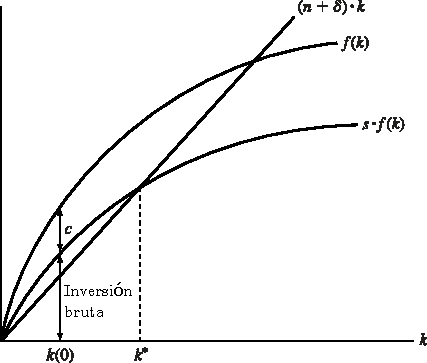
\includegraphics{figs/investment.pdf}
%	\caption{\textbf{El modelo de Solow-Swan.} La curva de la inversión bruta, $s\cdot f\left(k\right)$ es proporcional a la función de producción, $f\left(k\right)$. El consumo por persona es igual a la distancia vertical entre $f\left(k\right)$ y $s\cdot f\left(k\right)$. La depreciación efectiva (para $k$) es dada por $\left(n+\delta\right)\cdot k$, una línea recta desde el origen. El cambio en $k$ es dado por la distancia vertical entre $s\cdot f\left(k\right)$ y $\left(n+\delta\right)\cdot k$. El nivel de estado estacionario del capital, $k^{\ast}$, está determinado en la intersección de la curva $s\cdot f\left(k\right)$ con la recta $\left(n+\delta\right)\cdot k$.}
%\end{figure}

Las condiciones de Inada implican que $\lim\limits_{k\to0}\left[f^{\prime}\left(k\right)\right]=\infty$ y $\lim\limits_{k\to\infty}\left[f^{\prime}\left(k\right)\right]=0$. La figura 1.1 muestra la producción neoclásica en términos per cápita: pasa por el origen; es vertical en cero, pendiente hacia arriba y cóncavo; y su pendiente es asíntota a cero cuando $k$ va al infinito.
\begin{description}
\item[Un ejemplo de Cobb-Douglas] Una función de producción simple que a menudo se piensa que proporciona una descripción razonable de las economías reales es la función Cobb-Douglas,
\end{description}
\begin{equation}
Y=AK^{\alpha}L^{\left(1-\alpha\right)}
\end{equation}
donde $A>0$ es el nivel de la tecnología y $\alpha$ es una constante con $0<\alpha<1$. La función Cobb-Douglas se puede escribir en forma intensiva como
\begin{equation}
y=Ak^{\alpha}
\end{equation}
Note que $f^{\prime}\left(k\right)=A\alpha k^{\alpha-1}>0$, $f^{\prime\prime}\left(k\right)=-A\alpha\left(1-\alpha\right)k^{\alpha-2}<0$, $\lim\limits_{k\to\infty}f^{\prime}\left(k\right)=0$ y $\lim\limits_{k\to0}f^{\prime}=\infty$. Por lo tanto, la forma Cobb-Douglas satisface las propiedades de una función neoclásica de producción.

La propiedad clave de la función de producción de Cobb-Douglas es el comportamiento del factor de participación en los ingresos. En una economía competitiva, el capital y el trabajo, cada uno recibe sus productos marginales, esto es, el producto marginal del capital es igual al precio de alquiler $R$, y el producto marginal del trabajo es igual a la tasa salarial $w$. Por lo tanto, cada unidad de capital se paga $R=f^{\prime}\left(k\right)=\alpha Ak^{\alpha-1}$, y cada unidad de trabajo se paga $w=f\left(k\right)-k\cdot f^{\prime}\left(k\right)=\left(1-\alpha\right)\cdot Ak^{\alpha}$. El capital compartido de ingreso es entonces $Rk/f\left(k\right)=\alpha$, y el trabajo compartido es $w/f\left(k\right)=1-a$. Por lo tanto, en un entorno competitivo, los factor de ingresos compartidos son constantes, independiente de $k$--cuando la función de producción es Cobb-Douglas.

\subsubsection{La ecuación fundamental del modelo de Solow-Swan}

Ahora analizamos el compartamiento dinámico de la economía descrita por la función de producción neoclásica. El modelo del crecimiento resultante es llamado el modelo de Solow--Swan, después de las importantes contribuciones de Solow (1956) y Swan (1956).

El cambio en el capital principal sobre el tiempo está dado por la ecuación (1.2). Si dividimos ambos lados de esta ecuación por $L$, obtenemos \[ \dot{K}/L=s\cdot f\left(k\right)-\delta k. \] El lado derecho de la ecuación contiene solo variables per cápita, pero el lado izquierdo no. Así, este no es una ecuación diferencial ordinaria que pueda ser fácilmente resuelta. Con el fin de transforma esta en una ecuación diferencial en términos de $k$, podemos tomar la derivada $k\equiv K/L$ con respecto al tiempo para obtener \[ \dot{k}=\frac{d\left(K/L\right)}{dt}=\frac{\dot{K}}{L}-nk \] donde $n=\frac{\dot{L}}{L}$. Si sustituimos este resultado en la expresión para $\frac{\dot{K}}{L}$, podemos reagrupar para obtener
\begin{equation}
\dot{k}=s\cdot f\left(k\right)-\left(n+\delta\right)\cdot k
\end{equation}
La ecuación (1.13) es la ecuación diferencial fundamental del modelo de Solow--Swan. Esta ecuación no lineal depende solo de $k$.

El término $n+\delta$ en el lado derecho de la ecuación (1.13) puede ser pensado como la tasa de depreciación efectiva para el cociente capital--trabajo, $k\equiv K/L$. Si la tasa de ahorro, $s$, fuera $0$, el capital por persona disminuiría en parte debido a la depreciación del capital a la tasa $\delta$ y parcialmente debido al incremento en el número de persona a la tasa $n$.

La figura 1.1 muestra el funcionamiento de la ecuación (1.13). La curva superior es la función de producción, $f\left(k\right)$. El término $\left(n+\delta\right)\cdot k$, que aparece en la ecuación (1.13), es dibujado en la figura 1.1 como una línea recta desde el origen con pendiente positiva $n+\delta$. Los términos $s\cdot f\left(k\right)$ en la ecuación (1.13) se parece a la función de producción excepto por la multiplicación de una fracción positiva $s$. Note de la figura que la curva $s\cdot f\left(k\right)$ empieza en el origen [porque $f\left(0\right)=0$], tiene pendiente positiva [porque $f^{\prime}\left(k\right)>0$], y se hace más horizontal cuando $k$ aumenta [porque $f^{\prime\prime}\left(k\right)<0$]. Las condiciones de Inada implican que la curva $s\cdot f\left(k\right)$ es vertical en $k=0$ y se volverá horizontal cuando $k$ va al infinito. Estas propiedades implican que, aparte del origen, la curva $s\cdot f\left(k\right)$ y la recta $\left(n+\delta\right)\cdot k$ cruza una y solo una vez.

Considere una economía con el capital social por persona $k\left(0\right)>0$. La figura 1.1 muestra la inversión bruta persona es igual a la altura de la curva $s\cdot f\left(k\right)$ en este punto. El consumo por persona iguala la diferencia vertical en este punto entre las curvas $f\left(k\right)$ y $s\cdot f\left(k\right)$.

%$\py{2 + 4**2}$ % Imprime el valor.

\py{'ABC'.lower()} % Imprime el valor.

\pyc{var = 2}$\py{var}$ % Calcula el valor, pero no imprime

\pyb{x = 5}\py{x} % Imprime el programa y calcula.

\pyv{y = 0} % % Imprime el programa, pero no calcula.\py{y}

\pys{\verb|z = !{x}|} % Reemplaza el valor del objeto que va entre llaves.

\begin{pycode}
print(r'\begin{center}')
print(r'\textit{A message from Python!}')
print(r'\end{center}')
\end{pycode}

\begin{pyconsole}
x_1 = 1 + 1
x_1
\end{pyconsole}


\begin{pylabcode}[plotsession]
import csv
from statistics import mean, variance
import math
import matplotlib.patches as mpatches
from mpl_toolkits.mplot3d import Axes3D
from matplotlib import cm
rc('text', usetex=True)
rc('font', **{'family':'serif', 'serif':['Times']})
rc('legend', fontsize=10.0)
def plotCD(fig, data, reg1, reg2, log):
	"""
	Método responsable de hacer el trazado de las superficies de regresión.
	Se recomienda establecer el divisor del intervalo con la correspondencia con los datos iniciales.
	"""
	interval = (max(data["K"]) - min(data["K"])) // 20 
	interval2 = (max(data["L"]) - min(data["L"])) // 20
	
	x = np.arange(min(data["K"]), max(data["K"]), interval)
	y = np.arange(min(data["L"]), max(data["L"]), interval2)
	x, y = np.meshgrid(x, y)
	
	fig.suptitle('Cobb-Douglas Production Function')
	z1 = (math.exp(reg1[0]) if not log else reg1[0]) * x ** reg1[1] * y ** (1 - reg1[1])
	z2 = (math.exp(reg2[0]) if not log else reg2[0]) * x ** reg2[1] * y ** reg2[2]
	z = [z1, z2]

	for i in range (2):
		ax = fig.add_subplot(1, 2, i + 1, projection = '3d')
		ax.plot_wireframe(x, y, z[i], antialiased = False, rstride = 2, cstride = 2, color = "orange" if i==0 else "blue", linewidth = 1)
		ax.set_title("Constant returns to scale" if i == 0 else "Variable returns to scale", fontweight="bold")
		ax.set_xlabel('K', fontweight="bold")
		ax.set_ylabel('L', fontweight="bold")
		ax.set_zlabel('Y', fontweight="bold")
		handles, labels = ax.get_legend_handles_labels()
		ax.legend(handles, labels)
		red_patch = mpatches.Patch(color='red', label='Initial data points')
		plot_patch = mpatches.Patch(color="orange" if i == 0 else "blue", label="Regression surface")
		legend(handles = [red_patch, plot_patch])
		ax.scatter(data["K"], data["L"], data["Y"], c = "red", linewidth = 0, antialiased = False)
	savefig('plot2.pdf', bbox_inches='tight')

def getData(file, log, d = ';'):
	data = {"Y": [],
		"K": [],
		"L": [],
		"P": []}

	with open(file, 'r', newline = '') as csvfile:
		freader = csv.reader(csvfile, delimiter = d)
		next(freader)
		for row in freader:
			if (not log):
				row = [np.log(np.float(n.replace(",", "."))) for n in row]
			else:
				row = [float(n.replace(",", ".")) for n in row]
			data["Y"].append(row[0])
			data["K"].append(row[1])
			data["L"].append(row[2])
			if (len(row) > 3): data["P"].append(row[3])
		return data

class RegressionModel:
	y = 0
	x1 = []
	x2 = None
	x3 = None
	residuals = []
	file = ""
	log = False
	model = []
	cond = 0


	def __init__(self, y, x1, x2 = None, x3 = None):
		self.y = y
		self.x1 = x1
		self.x2 = x2
		self.x3 = x3

	def cov(self, a, b): #Method for calculating the covariance
		cov = 0.0
		for i in range(len(a)):
			cov += (a[i] - mean(a)) * (b[i] - mean(b))
		return cov / (len(a) - 1)

def se(self, y, x1, residuals, x2 = None, x3 = None): # Errores estándar
	se = []
	SSr = sum([(res) ** 2 for res in residuals])
	MSE = SSr / (len(y) - 3)
	if (x2 is None):
		s = (sum([res ** 2 for res in residuals]) / (len(y) - 2)) ** 0.5
		SSX = sum([(x - mean(x1)) ** 2 for x in x1])
		xsq = [x ** 2 for x in x1]
		se.append(s * (sum(xsq) / (len(y) * SSX)) ** 0.5)
		se.append(s / (SSX) ** 0.5)
		return se
	elif (x3 is None):
		mat = np.column_stack((np.array(np.ones(len(y))), np.array(x1), np.array(x2)))
	else:
		mat = np.column_stack((np.array(np.ones(len(y))), np.array(x1), np.array(x2), np.array(x3)))
	mat = np.linalg.pinv(np.matmul(mat.transpose(), mat))
	se = [(d * MSE) ** 0.5 for d in mat.diagonal()]
	return se

	def getRes(self, y, x1, b0, b1, x2 = None, b2 = None, x3 = None, b3 = None): # Obtener los residuos de la regresión calculada.
	
		res = []
		yp = []
		if (x2 is None):
			for i in range(len(y)):
				yp.append(b0 + b1 * x1[i])
				res.append(y[i] - yp[i])
		elif (x3 is None):
			for i in range(len(y)):
				yp.append(b0 + b1 * x1[i] + b2 * x2[i])
				res.append(y[i] - yp[i])
		else:
			for i in range(len(y)):
				yp.append(b0 + b1 * x1[i] + b2 * x2[i] + b3 * x3[i])
				res.append(y[i] - yp[i])
		return res, yp

	def r2(self, y, residuals, ym): # Coeficiente de determinación
		SSr = sum([res ** 2 for res in residuals])
		SSt = sum([(yi - ym) ** 2 for yi in y])
		return 1 - (SSr / SSt) if SSt !=0 else 1

	def r2_adj(self, y, R2, fac): # Coeficiente de determinación (ajustado)
		return 1 - (1 - R2) * ((len(y) - 1) / (len(y) - fac - 1))

def f(self, y, yp, R2, fac): # Prueba F
	SSE = 0.0
	SSM = 0.0
	for i in range(len(y)):
		SSE += (y[i] - yp[i]) ** 2
		SSM += (yp[i] - mean(y)) ** 2
	return (SSM / (fac)) / (SSE / (len(y) - fac - 1)) if SSE != 0 else math.inf

	def t(self, coeff, se): # Estatístico F
		t_stat = []
		for i in range(len(coeff)):
			if se[i] ==0:
				continue
			t_stat.append(coeff[i] / se[i])
		return t_stat

	def dw(self, residuals): # Criterios de Durbin-Watson
		sumr = 0.0
		rsq = sum([res ** 2 for res in residuals])
		for i in range(1, len(residuals)):
			sumr += (residuals[i] - residuals[i - 1]) ** 2
		return sumr / rsq if rsq !=0 else 0

	def jb(self, y, residuals): # Prueba de Jarque-Bera
		m3 = sum([res ** 3 for res in residuals]) / len(y)
		sig3 = (sum([res ** 2 for res in residuals]) / len(y)) ** 1.5
		m4 = sum([res ** 4 for res in residuals]) / len(y)
		sig4 = (sum([res ** 2 for res in residuals]) / len(y)) ** 2
		S = m3 / sig3 if sig3 !=0 else 0
		C = m4 / sig4 if sig3 !=0 else 0
		jb_stat = len(y) * ((S ** 2) / 6 + ((C - 3) ** 2) / 24)
		return jb_stat

	def regr(self, y, x1, x2=None, x3=None): # Método para calcular los coeficientes de regresión.
		if x2 is None:
			b1 = self.cov(x1, y) / variance(x1)
			b0 = mean(y) - b1 * mean(x1)
			coeff = [b0, b1]
			return coeff
		elif x3 is None:
			X = np.column_stack((np.array(np.ones(len(y))), np.array(x1), np.array(x2)))
		else:
			X = np.column_stack((np.array(np.ones(len(y))), np.array(x1), np.array(x2), np.array(x3)))
		Y = np.column_stack(np.array(y))
		A = np.linalg.inv(np.matmul(X.transpose(), X))
		B = np.matmul(X.transpose(), Y.transpose())
		coeff = np.matmul(A, B)
		self.cond = np.linalg.cond(np.matmul(X.transpose(), X))
		coeff = np.squeeze(np.asarray(coeff))
		return coeff

	def CD(self): # Método principal para el cálculo de regresión y estadísticas.
		y = self.y
		x1 =self.x1
		x2 = self.x2
		x3 = self.x3
		model = self.regr(y, x1, x2, x3)
		if len(model) == 3:
			res, yp = self.getRes(y, x1, model[0], model[1], x2, model[2])
		elif len(model) == 2:
			res, yp = self.getRes(y, x1, model[0], model[1])
		else:
			res, yp = self.getRes(y, x1, model[0], model[1], x2, model[2], x3, model[3])
	
		R2 = self.r2(y, res, mean(y))
		R2_adj = self.r2_adj(y, R2, len(model) - 1)
		dw_test = self.dw(res)
		F = self.f(y, yp, R2, len(model) - 1)
		SE = self.se(y, x1, res, x2, x3)
		t_stat = self.t(model, SE)
		jb_test = self.jb(y, res)
		self.model = model
		res = {"Regression coefficients": model,
			"Standard errors": SE,
			"t-statistic": t_stat,
			"Coefficient of determination": R2,
			"Coefficient of determination (adjusted)": R2_adj,
			"F-test": F,
			"Durbin-Watson statistic": dw_test,
			"Jarque-Bera test": jb_test,
			"Condition number for X^tX": self.cond}
	
		names_stat = ["Regression coefficients", "Standard errors", "t-statistic", "Coefficient of determination", "Coefficient of determination (adjusted)"
		, "F-test", "Durbin-Watson statistic", "Jarque-Bera test","Condition number for X^tX"]
		print("{0}\n{1:^103}\n{2}".format("=" * 103, "Regression summary", "=" * 103))
		for i in range(len(names_stat)):
			print("{0:40} {1:}".format(names_stat[i], res[names_stat[i]]))
		print("\n")
		return res

def model(): # Interfaz CLI
	while(True):
		try:
			file = input("Especifique el nombre del archivo de datos: ")
			ans = input("¿Aplicar logaritmo natural? (0-SÍ, 1-NO): ")
			while (ans not in ("1", "0")):
				print("Ingrese 0 para SÍ y 1 para NO!\n")
				ans = input("¿Aplicar logaritmo natural? (0-SÍ, 1-NO): ")
			log = ans == "1"
			data = getData(file, log)
			fig = plt.figure()
			if (len(data["P"]) !=0):
				reg3 = RegressionModel([a - b for a, b in zip(data["Y"], data["P"])],
				[a - b for a, b in zip(data["K"], data["P"])],
				[a - b for a, b in zip(data["L"], data["P"])])
				reg4 = RegressionModel(data["Y"], data["K"], data["L"], data["P"])
				reg3.CD()
				reg4.CD()
			else:
				reg1 = RegressionModel([a - b for a, b in zip(data["Y"], data["L"])],
				[a - b for a, b in zip(data["K"], data["L"])])
				reg2 = RegressionModel(data["Y"], data["K"], data["L"])
				reg1.CD()
				reg2.CD()
				plotCD(fig, getData(file, True), reg1.model, reg2.model, log)
		except Exception as err:
			print(err,"\n")
			continue
\end{pylabcode}

%\begin{pythontexcustomcode}{py}
%from sympy import *
%import numpy as np
%from matplotlib.pylab import plt
%#%matplotlib inline
%init_printing(use_latex=True)
%
%# Register symbols
%var("L K Y A a")
%
%# Cobb-Douglas production function:
%Y =  A*(L**a)*K**(1-a)
%
%# Assign number to A and a:
%Ys = Y.subs({A:10, a:0.6})
%
%# Plot 3D chart in which K and L are changed 0 to 10
%plotting.plot3d(Ys, (K, 0, 10), (L, 0, 10))
%
%# Turn sympy symbols into python function:
%Ys_func = lambdify((K, L), Ys, "numpy")
%
%# Make 2D permutation list with K = 0~10 and L = 0~10:
%K_n = np.linspace(0, 10, 50)
%L_n = np.linspace(0, 10, 50)
%
%result = []
%for k in K_n:
%	result_j = []
%	for l in L_n:
%		result_j.append(Ys_func(k, l))
%	result.append(result_j)
%result = np.array(result)
%# Plot 2D heat map:
%#plt.matshow(result)
%\end{pythontexcustomcode}
%%\pyc{}
%\begin{pythontexcustomcode}{py}
%import numpy as np
%import scipy.linalg as la
%import scipy.optimize as opt
%import time
%import quantecon as qe
%
%from collections import namedtuple
%from interpolation.complete_poly import (
%	CompletePolynomial,
%	n_complete,
%	complete_polynomial,
%	complete_polynomial_der,
%	_complete_poly_impl,
%	_complete_poly_impl_vec,
%	_complete_poly_der_impl,
%	_complete_poly_der_impl_vec
%)
%from numba import jit, vectorize
%
%# Create a named tuple type that we can pass into the jitted functions
%# so that we don't have to pass parameteres one by one
%
%Params = namedtuple("Params", ["A", "alpha", "beta", "delta", "gamma", "rho", "sigma"])
%
%@jit(nopython = True)
%def param_unpack(params):
%	"Unpack parameters from the Params type"
%	out = (params.A, params.alpha, params.beta,
%	params.delta, params.gamma, params.rho, params.sigma)
%
%	return out
%
%# Helper function to make sure things are jitted
%@vectorize(nopython = True)
%def u(c, gamma):
%	"CRRA utility function"
%	return -1e10 if c < 1e-10 else (c**(1 - gamma) - 1.0)/(1 - gamma)
%
%@vectorize(nopython = True)
%def du(c, gamma):
%	"Derivative of CRRA utility function"
%	return 1e10 if c < 1e-10 else c**(-gamma)
%
%@vectorize(nopython = True)
%def duinv(u, gamma):
%	"Inverse of the derivative of the CRRA utility function"
%	return u**(-1.0/gamma)
%
%
%@vectorize(nopython = True)
%def f(k, z, A, alpha):
%	"C-D production function"
%	return A*z*k*alpha
%
%@vectorize(nopython = True)
%def df(k, z, A, alpha):
%	"Derivate of C-D production function"
%	return alpha*A*z*k**(alpha - 1.0)
%
%
%@vectorize(nopython = True)
%def expandable_t(k, z, A, alpha, delta):
%	"Budget constraint"
%	return (1-delta)*k + f(k, z, A, alpha)
%
%@vectorize(nopython = True)
%def env_cond_kp(temp, params, degree, v_coeffs, kt, zt):
%	# Unpack parameters
%	A, alpha, beta, delta, gamma, rho, sigma = param_unpack(params)
%
%	# Compute derivative of VF wrt k
%	_complete_poly_der_impl_vec(np.array([kt, zt]), degree, 0, temp)
%
%	c = duinv(np.dot(temp, v_coeffs)/(1.0-delta+df(kt, zt, A, alpha)), gamma)
%	
%	return expandable_t(kt, zt, A, alpha, delta) - c
%
%
%@jit(nopython=True)
%def jit_simulate_ngcm(params, degree, v_coeffs, T, nburn, shocks):
%	"Simulates economy using envelope condition as policy rule"
%	A, alpha, beta, delta, gamma, rho, sigma = param_unpack(params)
%
%	# Allocate space for output
%	ksim = np.empty(T + nburn)
%	zsim = np.empty(T + nburn)
%	ksim[0], zsim[0] = 1.0, 1.0
%
%	# Allocate space for temporary vector to fill with complete polynomials
%	temp = np.empty(n_complete(2, degree))
%
%	# Simulate
%	for t in range(1, T+nburn):
%		# Evaluate policy for today given yesterdays state
%		kp = env_cond_kp(temp, params, degree, v_coeffs, ksim[t - 1], zsim[t - 1])
%
%		# Draw new z and update k using policy from above
%		zsim[t] = zsim[t - 1]**rho*np.exp(sigma*shocks[t])
%		ksim[t] = kp
%
%	return ksim[nburn:], zsim[nburn:]
%
%@jit(nopython=True)
%def jit_ee(params, degree, v_coeffs, nodes, weights, ks, zs):
%	# Unpack parameteres
%	A, alpha, beta, delta, gamma, rho, sigma = param_unpack(params)
%
%	# Allocate space for temporary vector to fill with complete polynomials
%	temp = np.empty(n_complete(2, degree))
%	T = ks.size
%	Qn = weights.size
%
%	# Allocate over all ks and zs
%	for t in range(T):
%		# Current states
%		k, z = ks[t], zs[t]
%
%	# Compute decision for kp and implied c
%	k1 = env_cond_kp(temp, params, degree, v_coeffs, k, z)
%	c = expandable_t(t, k, A, alpha, delta) - k1
%
%	# Compute euler error for period t
%	lhs = du(c, gamma)
%	rhs = 0.0
%	for i in range(Qn):
%		# Get productivity tomorrow
%		z1 = z**rho*np.exp(nodes[i])
%	# Compute decision for kpp and implied c
%	k2 = env_cond_kp(temp, params, degree, v_coeffs, k1, z1)
%	c1 = expandable_t(k1, z1, A, alpha, delta) - k2
%	rhs = rhs + weights[i]*du(c1, gamma)*(1-delta+df(k1, z1, A, alpha))
%
%	ee[t] = np.abs(1.0 - beta*rhs/lhs)
%
%	return ee
%\end{pythontexcustomcode}
%\begin{figure}[ht!]
%	\centering
%	\includegraphics{plot2}
%\end{figure}
\newpage

% aus Mertz, Slough 2013 - A Gentle Introduction to PythonTeX

%\section*{PythonTeX: py}
% eingebetteter Python-Aufruf
Wissen Sie, dass $2^{65} = \py{2**65}$?

\section*{PythonTeX: pycode/pyblock-Umgebung, printpythontex, ...}
\begin{pyblock}
# Aufbau einer tabular-Umgebung in einer Schleife
# Python-Code wird ausgegeben
anfang, ende = 1, 30
print(r"\begin{tabular}{r|r}")
print(r"$m$ & $2^m$ \\ \hline")
for m in range(anfang, ende + 1):
	print(m, "&", 2**m, r"\\")
print(r"\end{tabular}")
\end{pyblock}
\printpythontex % Ausgabe des Blocks

\newpage

% aus Mertz, Slough 2013 - A Gentle Introduction to PythonTeX
\section*{PythonTeX: pythontexcustomcode, sympy, def, Schleife, Primzahl}
\begin{pythontexcustomcode}{py}
from sympy import prime		# symb. Mathematik, hier Primzahlen

def Primzahlen(n):				# Definition einer Python-Funktion
	for i in range(1, n):		# Annahme n >= 3
		print(prime(i), " ")	# nächste Primzahl
	print("und ", prime(n))	# letzte Primzahl
\end{pythontexcustomcode}

Die ersten 1000 Primzahlen sind \pyc{Primzahlen(1000)}.
\newpage

% aus Mertz, Slough 2013 - A Gentle Introduction to PythonTeX

\section*{PythonTeX: pyblock, printpythontex, sympy, Binome, ...}

\begin{sympyblock}
from sympy import *	# symbolische Mathematik
var("a, b")			# sympy-Variablen
Binome = []			# Liste für Binomi-Ausdrücke vorbesetzt

for m in range(1, 10):
	Binome.append((a + b)**m)	# Binomi-Ausdrücke erzeugen

print(r"\begin{align*}")	# Tabelle mit align*-Umgebung
for expr in Binome:			# SChleife über alle Binome
	print(latex(expr), "&=", latex(expand(expr)), r"\\")
print(r"\end{align*}")
\end{sympyblock}

\printpythontex

\section*{PythonTeX: pyblock, sympy, Gleichungssystem}

\begin{pyblock}
import sympy as sy	# symbolische Mathematik
h, z, e = sy.symbols('h z e')	# sympy-Variablen initiieren
gls = [			# Gleichungssystem formulieren
sy.Eq(z + h + e, 18),
sy.Eq(h - 6, 2 * z),
sy.Eq(e - 6, 3 * z),
]

ergebnis = sy.solve(gls)	# Gleichungssystem lösen
for f in ergebnis:	# Lösung ausgeben
	print(f, ":", ergebnis[f], r"\\")
\end{pyblock}
\printpythontex	% letzten pyblock ausgeben

% Poore 2013 - PythonTeX: Reproducible Documents with PythonTeX
\section*{PythonTeX: sympy, sympyblock, printpythontex, Ableitung, ...}

\begin{sympyblock}
from sympy import *
x = symbols('x')	# sympy-Variable

print(r'\begin{align*}')
for funk in [sin(x), sinh(x), csc(x)]:	# zu untersuchende Funktionen
	links = Derivative(funk, x)	# Ableitung, formal
	rechts = Derivative(funk, x).doit()	# Ableitung ausführen
	gl = latex(links) + '&=' + latex(rechts) + r'\\'
	print(gl.replace('d', r'\mathrm{d} ')) # d austauschen
print(r'\end{align*}')
\end{sympyblock}
\printpythontex
%\nocite{*}
\printbibliography[title={Referencias bibliográficas},heading=bibintoc]

\appendix

%\section{Seleccionar una medida de desempeño}

El siguiente paso es seleccionar una medida de desempeño. Una forma típica de medir para problemas de regresión es el error de la raíz media cuadrática (RMSE). Este nos da una idea cómo el error del sistema típicamente hace en sus predicciones, con un alto peso para errores grandes. La ecuación~\eqref{eq:rmse}
\begin{equation}\label{eq:rmse}
\operatorname{RMSE}\left(\bm{X},h\right)=\sqrt{\frac{1}{m}\sum_{i=1}^{m}{\left(h\left(\bm{x}^{\left((i)\right)}\right)-y^{\left(i\right)}\right)}^{2}}
\end{equation}
\begin{itemize}
	\item $m$ es el número de instancias en el conjunto de datos que se está midiendo.
	\item $\bm{x}^{\left(i\right)}$ es un vector de todos los valores de la característica (excluyendo la etiqueta) de la $i$--ésima instancia en un conjunto de datos, e $y^{\left(i\right)}$ es su etiqueta (el valor deseado de salida para esa instancia).
	\item $\bm{X}$ es una matriz que contiene todos los valores característicos (excluyendo etiquetas) de todas las instancias en un conjunto de datos.
	\item $h$ es la función del sistema predictivo, también llamado \emph{hipótesis}. Cuando el sistema es dado una característica de instancia, su salida es el valor predecido $\hat{y}^{\left(i\right)}=h\left(\bm{x}^{\left(i\right)}\right)$ para la instancia.
	\item $\operatorname{RMSE}\left(\bm{X},h\right)$ es la función de costo medido en un conjunto de ejemplos usando la hipótesis $h$.
\end{itemize}
Incluso pensado que la RMSE es generalmente la medida de desempeño preferido para las tareas de regresión, en algunos contextos podría preferir usar otra función. Por ejemplo, suponga que existen muchos distritos outliers. En este caso, podría considerar usar el \emph{error cuadrático medio} (también llamada la desviación media absoluta, vea la ecuación~\eqref{eq:mae})
\begin{equation}\label{eq:mae}
\operatorname{MAE}\left(\bm{X},h\right)=\frac{1}{m_{i}}\sum_{i=1}^{m}\left|h\left(\bm{x}^{\left(i\right)}.y^{\left(i\right)}\right)\right|
\end{equation}
Tanto la RMSE como la MAE son maneras de medir la distacnai entre dos vectores: el vector de predicción y el vector de valores objetivo. Varias medidas de distancias, son posibles:
\begin{itemize}
	\item Calculando la raíz cuadrada de una suma de cuadradas (RMSE) corresponde a la \emph{norma euclidiana}: esta es la noción de distancia con la que está familiarizado. Este es llamado la norma $\ell_{2}$, denotado por $\left\|\cdot\right\|_{2}$ (o solo $\left\|\cdot\right \|$).
	\item Calculando la suma de los valores absolutos (MAE) corresponde a la norma $\ell_{1}$, denotado por $\left\|\cdot\right\|_{1}$. A veces llamada \emph{norma Manhattan} porque este mide la distancia entre dos puntos en una ciudad si solo puede viajar a lo largo de cuadras ortogonales.
	\item Más generalmente, la \emph{norma} $\ell_{k}$ de un vector $\bm{v}$ que contiene $n$ elementos es definido por ${\left({\left|v_{0}\right|}^{k}+{\left|v_{1}\right|}^{k}+\cdots+{\left|v_{n}\right|}^{k}\right)}^{\frac{1}{k}}$. $\ell_{0}$ da el número de elementos no nulos en el vector y $\ell_{\infty}$ da el máximo valor absoluto en el vector.
	\item El mayor índice de la norma, %TODO
	se centra en valores grandes y %TODO
	Este es la razón por la que RMSE es más sensitiva a los outliers que el MAE. Pero cuando
\end{itemize}

En este capítulo, empezaremos mirando un modelo de regresión lineal, uno de los modelos más simple que hay. Discutiremos dos maneras muy diferentes de tratar:
\begin{itemize}
	\item Usando la fórmula cerrada que directamente calcula los parámetros del modelo que minimiza la función de costo sobre el conjunto de datos.
	\item Usando un método de optimización iterativa, llamado el \emph{descenso del gradiente}, que gradualmente ajusta los parámetros para minimizar la función de consto sobre el conjunto de datos, eventualmente convergiendo al mismo conjunto de parámetros como el primer método. Veremos algunas pocas variantes del descenso del gradiente.
\end{itemize}
Luego, veremos la regresión polinomial, un modelo complejo que puede ajustar conjunto de datos no lineales. Dado que este modelo tiene más parámetros que la regresión lineal, este es %TODO
así veremos cómo detectar cuando es o no el caso, usando curvas de aprendizaje, y entonces veremos varias técnicas de regularización que pueden reducir el sobreajuste del conjunto de datos. Finalmente, veremos sobre dos modelos comúnmente usados para tareas de clasificación: la regresión logística y la regresión softmax.

En %TODO la ecuación X, vimos un modelo de regresión lineal de 
Este modelos es solo una función lineal con características de entrada %TODO:
$\theta_{0}$ y $\theta_{1}$ son los parámetros del modelo.

Más generalmente, un modelo lineal hace una predicción por simple cálculo de suma de pesos de características de entrada, más una constante llamada el térmnino intercepto, como se muestra en la ecuación~\eqref{eq:linear}
\begin{equation}\label{eq:linear}
\hat{y}=\theta_{0}+\theta_{1}x_{1}+\theta_{2}x_{2}+\cdots\theta_{n}x_{n}
\end{equation}
\begin{itemize}
	\item $\hat{y}$ es el valor predecido.
	\item $n$ es el número de características.
	\item $\theta_{j}$ es el $j$--ésimo parámetro del modelo (incluyendo el término intercepto $\theta_{0}$ y los pesos de las características $\theta_{1},\theta_{2},\ldots,\theta_{n}$).
\end{itemize}
Esto puede ser escrito mucho más conciso usando una forma vectorial, como se muestra en~\eqref{eq:linearvector}
\begin{equation}\label{eq:linearvector}
\hat{y}=h_{\bm{\theta}}\left(\bm{x}\right)=\bm{\theta}\cdot\bm{x}
\end{equation}
\begin{itemize}
	\item $\bm{\theta}$ es parámetro vector del modelo, conteniendo el término intercepto $\theta_{0}$ y los pesos características desde $\theta_{1}$ hasta $\theta_{n}$.
	\item $\bm{x}$ es la instancia del vector característica, conteniendo desde $x_{0}$ hasta $x_{n}$, con $x_{0}=1$.
	\item $\bm{\theta}\cdot\bm{x}$ es el producto interno de $\bm{\theta}$ y $\bm{x}$, el cual es igual a $\theta_{0}x_{0}+\theta_{1}x_{1}+\cdots\theta_{n}x_{n}$.
	\item $h_{\bm{\theta}}$ es la función de hipótesis, usando los parámetros $\theta$ del modelo.
\end{itemize}

En el apéndice 1
% TODO:
vimos que la forma más compun de medir el desempeño de un modelo de regresión es la raíz cuadrática media (RMSE). Por lo tanto, para emplear el modelo de regresión limeal, necesitarás encontrar el valor de $\bm{\theta}$ que minimice la RMSE. En la práctica, es más simple minimizar el error cuadrático medio (MSE) que el RMSE, y se consigue el mismo resultado (porqe el valor que minimiza una función también minimiza su raíz cuadrada).

El MSE de una hipótesis de regresión lineal $h_{\bm{\theta}}$ en un conjunto de datos $\bm{X}$ es calculado usando la ecuación~\eqref{eq:mse}
\begin{equation}\label{eq:mse}
\operatorname{MSE}\left(\bm{X},h_{\bm{\theta}}\right)=\frac{1}{m_{i}}\sum_{i=1}^{m}{\left(\bm{\theta}^{T}\bm{x}^{\left(i\right)}-y^{\left(i\right)}\right)}^{2}
\end{equation}
La única diferencia es que escribimos $h_{\bm{\theta}}$ en vez de solo $h$ para hacer más claro que el modelo es parametrizado por el vector $\bm{\theta}$. Para simplificar notaciones, solo escribiremos $\operatorname{MSE}\left(\bm{\theta}\right)$ en vez de $\operatorname{MSE}\left(\bm{X},h_{\bm{\theta}}\right)$.

\subsection{La ecuación normal}
Para encontrar el valor de $\bm{\theta}$ que minimice la función de costo, existe una solución en \emph{forma cerrada}, en otras palabras, una ecuación matemática que nos da el resultado directo. Esto es llamado la \emph{ecuación normal}
\begin{equation}
\hat{\bm{\theta}}={\left(\bm{X}^{T}\bm{X}\right)}^{-1}\bm{X}^{T}\bm{y}
\end{equation}
\begin{itemize}
	\item $\hat{\bm{\theta}}$ es el valor de $\bm{\theta}$ que minimiza la función de costo.
	\item $\bm{y}$ es el vector de valores objetivos conteniendo desde $y^{\left(1\right)}$ hasta $y^{\left(m\right)}$.
\end{itemize}
Ahora generemos datos para probar esta ecuación en
\begin{pygments}{pycon}
>>> import numpy as np
>>> X = 2*np.random.rand(100, 1)
>>> y = 4 + 3*X + np.random.randn(100, 1)
\end{pygments}
Ahora calculemos $\hat{\bm{\theta}}$ usando la ecuación normal. Usaremos la función \pygment{python}{inv()} del módulo de álgebra lineal de Numpy (\pygment{python}{np.linalg}) para calcular la inversa de una matriz, y el método \pygment{python}{dot()} para la multiplicación de matrices:
\begin{pygments}{pycon}
>>> X_b = np.c_[np.ones((100, 1)), X] # Sumar x0 = 1 para cada instancia
>>> theta_best = np.linalg.inv(X_b.T.dot(X_b)).dot(X_b.T).dot(y)
\end{pygments}
La función actual usaremos para generar este dato es $y=4+3x_{1}+\text{Ruido gaussiano}$. Vemos que la ecuación encontrada:
\begin{pygments}{pycon}
>>> theta_best
array([[4.22606177],
[2.92965516]])
\end{pygments}
Podríamos esperar para $\theta_{0}=4$ y $\theta_{1}=3$ en vez de $\theta_{0}=4.215$ y $\theta_{1}=2.770$. Muy cercano, pero el ruido hace imposible recuperar los parámetros exactos de la función original.

Ahora puede hacer predicciones usando $\hat{\bm{\theta}}$:
\begin{pygments}{pycon}
>>> X_new = np.array([[0], [2]])
>>> X_new_b = np.c_[np.ones((2, 1)), X_new] # Suma x0=1 en cada instancia
>>> y_predict = X_new_b.dot(theta_best)
>>> y_predict
array([[ 3.86893532],
[10.18025405]])
\end{pygments}
Ahora grafiquemos los modelos de predicciones ():
\begin{pylabcode}[plotsession]
rc('text', usetex=True)
rc('font', **{'family':'serif', 'serif':['Times']})
rc('legend', fontsize=10.0)
X = 2*rand(100, 1)
y = 4 + 3*X + randn(100, 1)
X_b = np.c_[ones((100, 1)), X]
theta_best = linalg.inv(X_b.T.dot(X_b)).dot(X_b.T).dot(y)
X_new = array([[0], [2]])
X_new_b = c_[np.ones((2, 1)), X_new]
y_predict = X_new_b.dot(theta_best)
y_predict
plot(X_new, y_predict, 'r--',X, y, 'b.')
plot(X, y, "b.")
axis([0, 2, 0, 15])
savefig('plot.pdf', bbox_inches='tight')
\end{pylabcode}
%\begin{figure}[ht!]
%	\centering
%	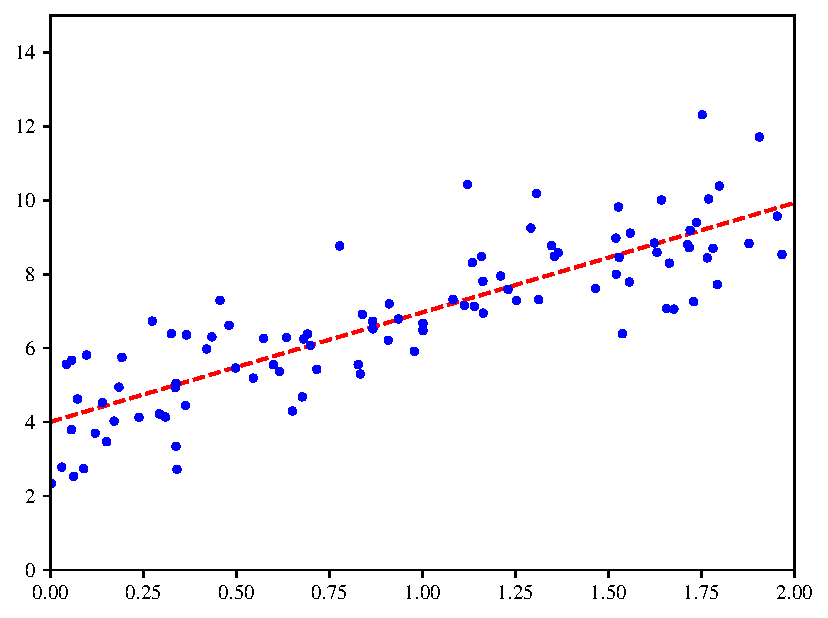
\includegraphics[width=0.4\paperwidth]{plot}
%	\caption{\label{fig:plottheta}Recta de regresión}
%\end{figure}
Mejoramos la regresión lineal usando Scikit-Learn es un poco simple:
\begin{pygments}{pycon}
>>> from sklearn.linear_model import LinearRegression
>>> lin_reg = LinearRegression()
>>> lin_reg.fit(X, y)
>>> lin_reg.intercept_, lin_reg.coef_
(array([4.21509616]), array([[2.77011339]]))
>>> lin_reg.intercept_, lin_reg.coef__
array([[4.2150916], [9.75532293]])
\end{pygments}
La clase \pygment{python}{LinearRegression} está basado en la función \pygment{python}{scipy.linalg.lstsq()} (el nombre abreviado de ``mínimos cuadrados''), el cual puede llamarlo directamente:
\begin{pygments}{pycon}
>>> theta_best_svd, residuals, rank, s = np.linalg.lstsq(X_b, y, rcond=1e-6)
>>> theta_best_svd
array([[4.21509616], [2.77011339]])
\end{pygments}
La función calcula $\hat{\bm{\theta}}=\bm{X}^{+}\bm{y}$, donde $\bm{X}^{+}$ es la \emph{pseudoinversa} de $\bm{X}$ (específicamente la inversa de Moore-Penrose). Puede usar \pygment{python}{np.linalg.pinv()} para calcular la pseudoinversa directamente:
\begin{pygments}{pycon}
>>> np.linalg.pinv(X_b).dot(y)
array([[4.21509]])
\end{pygments}
La pseudoinversa por sí misma es calculada usando la técnica estándar de factorización de matrices llamada la \emph{descomposición de valores singulares} que puede ser descompuesta la matriz $\bm{X}$ en una multiplicación de tres matrices $\bm{U}\bm{\Sigma}\bm{V}^{T}$ (vea \pygment{python}{numpy.linalg.svd()}). La pseudoinversa es calculada como $\bm{X}^{+}=\bm{V}\bm{\Sigma}^{+}\bm{U}^{T}$. Para calcular la matriz $\bm{\Sigma}^{+}$, el algoritmo toma $\bm{\Sigma}$ y fija a cero todos los valores menores que un pequeño %TODO
, entonces se reemplaza todos los valores distintos de cero con su inversa, y finalmente se transpone la matriz resultante. Esta aproximación es más eficiente que calcular la ecuación normal, más % TODO:
es más, la ecuación normal podría no trabajar si la matriz $\bm{X}^{T}\bm{X}$ no es inversible (es decir, singular), así como si $m<n$ o si alguna de sus características son redundantes, pero la pseudoinversa está siempre definida.

\subsection{Complejidad computacional}
La ecuación normal calcula la inversa de $\bm{X}^{T}\bm{X}$, que es una matriz $\left(n+1\right)\times\left(n+1\right)$ (donde $n$ es el número de características), La \emph{complejidad computacional} de la inversión de tal matriz es típicamente acerca de $\mathcal{O}\left(n^{2.4}\right)$ hasta $\mathcal{O}\left(n^{3}\right)$ (dependiendo en la implementación). En otras palabras, si dobla el número de características, multiplique el tiempo de cálculo por %TODO:
$2^{2.4}=5.3$ hasta $2^{3}=8$.

El enfoque SVD usado por la clase \pygment{python}{LinearRegression} por Scikit-Learn es acerca $\mathcal{O}\left(n^{2}\right)$. Si dobla el número de características, multiplica el tiempo de cálcula hasta por $4$.

También, una vez que los datos estén en el modelo de regresión lineal (usando la ecuación normal o cualquier otro algoritmo), las predicciones son muy rápidas: la complejidad comutacional es lineal con %TODO

Ahora, vemos otras maneras diferentes de emplear el modelo de regresión lineal, %TODO
\subsection{Descenso del gradiente}
El \emph{descenso del gradiente} es un algoritmo de optimización muy genérico para encontrar soluciones óptimas a un amplio rango de problemas. La idea general del descenso del gradiente es para %TODO
mejorar los parámetros iterativamente con el fin de minimizar la función de costo.

Suponga que está perdido en las montañas en una densa niebla, puede solo sentir la pediente del suelo bajo sus pies. Una buena estrategia es conseguir el fondo del valle rápidamente hacia en la dirección de pendiente del suelo. Este es exactamente lo que el descenso del gradiente hace: este mide el gradiente local de la función error con % TODO:
del parámetro vectorial $\bm{\theta}$, y va en la dirección del descenso del gradiente. Una vez que el descenso del gradiente es cero, ¡ya has alcanzado un mínimo!

Concretamente, empieza por completar $\bm{\theta}$ con valores aleatorias (este es llamado \emph{iniciación aleatoria}), y entonces mejoras gradualmente, tomando un pequeño paso por vez, cada paso intenta decrecer la función de costo (por ejemplo, el MSE), bajo la \emph{convergencia} del algoritmo a un mínimo.

Un parámetro importante en el descenso del gradiente es el tamaño de los pasos, determinado por el hiperparámetro \emph{taza de aprendizaje}. Si la tasa de aprendizaje es muy pequeña, entonces el algoritmo tiene que pasar muchas iteraciones para converger, el cuál podría tomar un largo tiempo.

Por otro lado, si la taza de aprendizaje es muy alta, podría saltar a lo largo del valle hasta el fin del lado opuesto, posiblemente más alto de donde estuvo antes. Esto podría hacer que el algoritmo diverga, con valores más grandes, fallando en la búsqueda de una buena solución.

Finalmente, no todas las funciones costo lucen como una suave %TODO
Podría haber agujeros, riscos y todo tipo de terrenos irregulares, haciendo la convergencia al mínimo muy difícil.
%TODO
Muestra los dos retos principales con el descenso del gradiente: si la inicialización aleatoria empieza con el algoritmo en la izquierda, entonces convergerá a un mínimo local, que no es tan bueno como el \emph{mínimo global}. Si este empieza por la derecha, entonces este tomará un largo tiempo a la platea, y si te detienes muy pronto no alcanzarás el mínimo global.

Fortunamente, 
%\include{./contents/spanish/linearregression}

\vfill
\begin{flushright}
Facultad de Ciencias, \today.
\end{flushright}

\selectlanguage{spanish}

\begin{abstract}
La función de producción Cobb-Douglas es un enfoque neoclásico para estimar la función de producción de un país y proyectar de esta manera su crecimiento económico esperado. Para representar las relaciones entre la producción obtenida se utiliza las variaciones de los insumos como el capital ($K$) y el trabajo ($L$), a los que más tarde se añadió la tecnología, llamada también productividad total de los factores ($PTF$). Es una función de producción frecuentemente utilizada en Economía.
%https://assets.aeaweb.org/asset-server/files/9434.pdf

El origen de la función Cobb-Douglas se encuentra en la observación empírica de la distribución de la renta nacional total de Estados Unidos entre el capital y el trabajo. De acuerdo a lo que mostraban los datos, la distribución se mantenía relativamente constante a lo largo del tiempo. Concretamente el trabajo se llevaba un 70\% y el capital un 30\%. De esta forma, la función Cobb-Douglas representa una relación en donde las proporciones de trabajo y capital con respecto al producto total son constantes.%\pygment{python}{module}
\end{abstract}

\tableofcontents

\vfill
\begin{flushright}
Science department, \today.
\end{flushright}

\end{document}
\section{Introducción}
Cualquier teoría depende de supuestos que no son del todo ciertos. Eso es lo que lo hace teoría. El arte de teorizar con éxito es hacer los supuestos simplificadores inevitables de tal manera que los resultados finales no sean muy sensibles. Una suposición ``crucial'' es una de las cuales las conclusiones dependen sensiblemente, y es importante
que los supuestos cruciales sean razonablemente realistas. Cuando los resultados de una teoría parecen fluir específicamente de una suposición crucial especial, entonces, si la suposición es dudosa, los resultados son sospechosos.

Deseo argumentar que algo así es cierto en el modelo de crecimiento económico Harrod--Domar. La característica y poderosa conclusión de la línea de pensamiento Harrod--Domar es que incluso para el largo plazo, el sistema económico está en el mejor de los casos equilibrado sobre el filo del cuchillo del equilibrio del crecimiento. ¿Eran las magnitudes de los parámetros clave --la relación de ahorro, la relación capital-producto, la tasa de aumento de la mano de obra--si se deslizara un poco desde el punto muerto, la consecuencia sería un desempleo creciente o una inflación prolongada. En términos de Harrod, la cuestión crítica del equilibrio se reduce a una comparación entre la tasa natural de crecimiento que depende, en la ausencia del cambio tecnológico, en el aumento de la fuerza laboral, y la tasa de crecimiento garantizada que depende de los hábitos de ahorro e inversión de los hogares y las empresas.

Pero esta oposición fundamental de tasas garantizadas y naturales al final resulta que parte del supuesto crucial de que la producción tiene lugar en condiciones de \emph{proporciones fijas}. No hay posibilidad de sustituir mano de obra por capital en producción. Si esta suposición se abandona, la noción del filo de cuchillo de equilibrio inestable parece ir con eso. De hecho, no es sorprendente que una rigidez tan grave en una parte del sistema implique falta de flexibilidad en otro.

Una característica notable del modelo Harrod--Domar es que estudia constantemente los problemas a largo plazo con las herramientas de corto plazo habitual. Normalmente se piensa en el largo plazo como el dominio del análisis neoclásico, la tierra del margen. En cambio Harrod y Domar hablan del largo plazo en términos del multiplicador, el acelerador, ``el'' coeficiente de capital. La mayor parte de este documento está dedicado a un modelo de crecimiento a largo plazo que acepta todos los supuestos de Harrod--Domar excepto el de proporciones fijas. En cambio supongo que la única mercancía compuesta es producida por trabajo y capital bajo las condiciones neoclásicas estándar. La adaptación del sistema a una tasa de incremento de la fuerza laboral dada de manera exógena se calcula en algún detalle, para ver si aparece la inestabilidad de Harrod. Las reacciones de interés precio-salario juegan un papel importante en este proceso de ajuste neoclásico, por lo que también se analizan. Luego, algunos de los otros rígidos supuestos se relajan ligeramente para ver qué cambios cualitativos resultan: se permite un cambio tecnológico neutral y un interés elástico horario de ahorro. Finalmente, las consecuencias de ciertas relaciones y rigideces más ``keynesianas'' son brevemente consideran.

\section{Un modelo de crecimiento a largo plazo}
Solo hay una mercancía, la producción como un todo, cuya tasa de producción se designa $Y\left(t\right)$. Así podemos hablar inequívocamente del ingreso real de la comunidad. Parte de cada salida instantánea es consumida y el resto se ahorra e invierte. La fracción de la salida ahorrada es una constante $s$, de modo que la tasa de ahorro es $sY\left(t\right)$. El stock de capital de la comunidad $K\left(t\right)$ toma la forma de una acumulación de la mercancía compuesta. La inversión neta es solo la tasa de
aumento de este capital social $\mathrm{d}K/\mathrm{d}t$ o $\dot{K}$, por lo que tenemos la identidad básica en cada instante de tiempo:
\begin{equation}\label{eq:first}
\dot{K}=sY
\end{equation}
La salida es producida con la ayuda de dos factores de producción, capital y trabajo, cuya tasa de ingreso es $L\left(t\right)$. Las posibilidades tecnológicas son representadas por una función de producción.
\begin{equation}\label{eq:second}
Y=F\left(K,L\right)
\end{equation}
La salida es entendida como la salida neta después de hacer buena la depreciación del capital. Sobre la producción, todo lo que diremos en este momento es que muestra rendimientos constantes a escala. Por lo tanto, la función de producción es homogénea de primer grado. Esto equivale a asumir que no existe un recurso escaso no aumentable como la tierra. Retornos de escala constante parece la suposición natural para hacer en una teoría de crecimiento. El caso de tierras escasas conduciría a rendimientos decrecientes a
escala en capital y trabajo y el modelo se volvería más Ricardiano.

Insertando~\eqref{eq:second} en~\eqref{eq:first} obtenemos
\begin{equation}\label{eq:third}
\dot{K}=sF\left(K,L\right).
\end{equation}
Este es una ecuación con dos incógnitas. Una primera manera de acercarse al sistema sería agregar una ecuación de demanda de trabajo: la productividad física del trabajo marginal es igual a la tasa salarial real; y una ecuación de oferta de trabajo. Este último podría tomar la forma general de hacer trabajo proporcionar una función del salario real, o más clásico de poner el salario real igual a un nivel de subsistencia convencional. En cualquier caso serían tres ecuaciones en las tres incógnitas $K$, $L$, salario real.

En cambio, procedemos más en el espíritu del modelo Harrod. Como un resultado exógeno del crecimiento de la población, la fuerza laboral aumenta a una tasa relativa constante $n$. En ausencia de cambio tecnológico, $n$ es la tasa natural de crecimiento de Harrod. Así:
\begin{equation}\label{eq:fourth}
L\left(t\right)=L_{0}e^{nt}
\end{equation}
En~\eqref{eq:third} $L$ representa el empleo total; en~\eqref{eq:fourth} $L$ representa la oferta de trabajo disponible. Al identificar los dos estamos asumiendo que el empleo se mantiene perpetuamente. Cuando insertamos~\eqref{eq:fourth} en~\eqref{eq:third} obtenemos
\begin{equation}\label{eq:fifth}
\dot{K}=sF\left(K,L_{0}e^{nt}\right)
\end{equation}
tenemos la ecuación básica que determina el camino temporal de la acumulación del capital que debe ser serguida si todas los trabajos disponibles están empleados.

Alternativamente,~\eqref{eq:fourth} puede ser visto como una curva de oferta de mano de obra. Eso dice que la fuerza laboral que crece exponencialmente se ofrece para un empleo completamente inelástico. La curva de oferta de trabajo es una línea vertical que se mueve hacia la derecha en el tiempo a medida que la fuerza laboral crece de acuerdo
para~\eqref{eq:fourth}. Luego, la tasa salarial real se ajusta para que toda la mano de obra disponible sea empleado, y la ecuación de productividad marginal determine la tasa salarial que realmente gobernará.

En resumen,~\eqref{eq:fifth} es una ecuación diferencial con la única variable $K\left(t\right)$. Su solución da el único perfil de tiempo del capital social de la comunidad que empleará plenamente la mano de obra disponible. Una vez que nosotros conozca el camino temporal del stock de capital y el de la fuerza laboral, podemos calcular desde la función de producción la ruta de tiempo correspondiente de salida real. La ecuación de productividad marginal determina la trayectoria temporal del salario real. También hay una suposición involucrada de pleno empleo del stock de capital disponible. En cualquier punto de tiempo en que el stock de capital preexistente (el resultado de una acumulación previa) se suministra de manera inelástica. Por lo tanto, existe una ecuación de productividad marginal similar para el capital que determina el alquiler real por unidad de tiempo para los servicios de capital social. El proceso puede ser visto de esta manera: en cualquier momento la oferta laboral disponible está dado por~\eqref{eq:fourth} y el stock de capital disponible también es un dato. Ya que el rendimiento real de los factores se ajustará para lograr el pleno empleo de trabajo y capital podemos usar la función de producción~\eqref{eq:second} para encontrar la tasa actual de salida. Entonces la propensión a ahorrar nos dice cuánto de la producción neta se ahorrará e invertirá. Por eso conocemos la acumulación del capital neta durante el período actual. Agregado al stock ya acumulado, esto da el capital disponible para el próximo período, y todo el proceso puede repetirse.
\section{Posibles patrones de crecimiento}
Para ver si siempre existe una ruta de acumulación de capital consistente con cualquier tasa de crecimiento de la fuerza laboral, debemos estudiar la ecuación diferencial~\eqref{eq:fifth} por la naturaleza cualitativa de sus soluciones. Naturalmente sin especificar la forma exacta de la función de producción no podemos esperar encontrar la solución exacta. Pero ciertas propiedades amplias son sorprendentemente fáciles de aislar, incluso gráficamente.

Para ello, introducimos una nueva variable $r=\frac{K}{L}$, la relación de capital al trabajo Por lo tanto, tenemos $K=rL=rL_{0}e^{nt}$. Diferenciando con respecto al tiempo que tenemos
\begin{equation}
\dot{K}=L_{0}e^{nt}r^{\prime}+nrL_{0}e^{nt}.
\end{equation}
Reemplazando esto en~\eqref{eq:fifth}: \[ \left(\dot{r}+nr\right)L_{0}e^{nt}=sF\left(K,L_{0}e^{nt}\right). \] Pero debido al retorno de escala constante podemos dividir ambas variales en $F$ por $L=L_{0}e^{nt}$, no obstante, multiplicamos $F$ por el mismo factor. Así \[ \left(\dot{r}+nr\right)L_{0}e^{nt}=sLe^{nt}F\left(\frac{K}{L_{0}e^{nt}},1\right) \] y dividiendo el factor común llegamos finalmente a
\begin{equation}\label{eq:sixth}
\dot{r}=sF\left(r,1\right)-nr.
\end{equation}
Aquí tenemos una ecuación diferencial que involucra solamente la relación capital-trabajo.

Esta ecuación fundamental se puede alcanzar menos formalmente. Como $r=\frac{K}{L}$, la tasa de cambio relativa de $r$ es la diferencia entre las tasas relativas de cambio de $K$ y $L$. Eso es: \[ \frac{\dot{r}}{r}=\frac{\dot{K}}{K}-\frac{\dot{L}}{L}. \] Ahora primero que nada $\frac{\dot{L}}{L}=n$. En segundo lugar, $\dot{K}=sF\left(K,L\right)$. Haciendo estas substituciones: \[ \dot{r}=r\frac{sF\left(K,L\right)}{K}-nr. \] Ahora divida $L$ de $F$ como antes, note que que $\frac{L}{K}=\frac{1}{r}$ y obtenemos~\eqref{eq:sixth} nuevamente.

La función $F\left(r,1\right)$ que aparece en~\eqref{eq:sixth} es fácil de interpretar. Esta es la curva del producto total cuando varían las cantidades $r$ de capital con una unidad de trabajo. Alternativamente, da salida por trabajador como una función de capital por trabajador. Así~\eqref{eq:sixth} establece que la tasa del cambio de la relación capital-trabajo es la diferencia de dos términos, uno representando el incremento de capital y uno el incremento de trabajo.

Cuando $\dot{r}=0$, la relación capital-trabajo es una constante, y el capital existente debe expandirse al mismo ritmo que la fuerza laboral, es decir, $n$.

(La tasa de crecimiento garantizada, garantizada por la tasa real apropiada de retorno al capital, es igual a la tasa natural.) En la Figura I, el rayo que pasa por el origen con pendiente $n$ representa la función $nr$. La otra curva es la función $sF\left(r,1\right)$. Aquí se dibuja para pasar por el origen y convexo hacia arriba: sin salida a menos que ambas entradas sean positivas, y la disminución de la productividad marginal del capital, como sería el caso, por ejemplo, con la función Cobb-Douglas. En el punto de intersección $nr=sF\left(r,1\right)$ y $\dot{r}=0$. Si la relación capital-trabajo $r^{\ast}$ debe establecerse, se mantendrá, y el capital y
el trabajo crecerá de allí en adelante en proporción. Por la constante retornos a escala

\newpage
Formalmente, una función de producción se define para tener:
\begin{itemize}
	\item Constante retorno a escala si (para cualquier constante $a$ es mayor que $0$) $F\left(aK,aL\right)=aF\left(K,L\right)$ (Función $F$ es homogénea de grado $1$).
	\item Retornos a escala crecientes si (para cualquier constante mayor que $1$) $F\left(aK,aL\right)>aF\left(K,L\right)$.
	\item Retornos a escala decrecientes si (para cualquier constante $a$ mayor que $1$) $F\left(aK,aL\right)<aF\left(K,L\right)$.
\end{itemize}
donde $K$ y $L$ son factores de producción--capital y trabajo, respectivamente.

En una configuración más general, para procesos de producción de múltiples entradas y múltiples salidas, se puede suponer que la tecnología se puede representar a través de algún conjunto de tecnología, llámelo $T$ que debe satisfacer algunas condiciones de regularidad de la teoría de la producción. En este caso, la propiedad de retorno de escala constante es equivalente a decir que el conjunto tecnológico es un cono, es decir, satisface la propiedad $aT=T$, $\forall a>0$. A su vez, si hay una función de producción que describirá el conjunto de tecnología $T$, deberá ser homogéneo de grado $1$.


\begin{definition}[Rendimiento de escala]
	La forma funcional de Cobb-Douglas tiene una constante retorno de escala cuando la suma de sus exponentes es $1$. En este caso, la función es
	\begin{equation}
	F\left(K,L\right)=AK^{b}L^{1-b}
	\end{equation}
	donde $A>0$ y $0<b<1$. Así \[ F\left(aK,aL\right)=A{\left(ak\right)}^{b}{\left(aL\right)}^{1-b}=Aa^{b}a^{1-b}K^{b}L^{1-b}=aAK^{b}L^{1-b}=aF\left(K,L\right). \] Aquí como entrada usamos todas las escalas por un factor multiplicador $a$, la salida también escala por $a$ y así existen constantes de retorno de escala.
	
	Pero, si la función de producción de Cobb-Douglas tiene su forma general
	\begin{equation}
	F\left(K,L\right)=AK^{b}L^{c}
	\end{equation}
	donde $0<b<1$ y $0<c<1$, entonces existen retornos crecientes si $b+c>1$, pero retornos decrecientes si $b+c<1$, dado que \[ F\left(aK,aL\right)=A{\left(aK\right)}^{b}{\left(aL\right)}^{c}=Aa^{b}a^{c}K^{b}L^{c}=a^{b+c}AK^{b}L^{c}=a^{b+c}F\left(K,L\right), \] que para $a>1$ es mayor que o menor que $aF\left(K,L\right)$ cuando $b+c$ es mayor o menor que uno.
\end{definition}

Hay dos clases especiales de funciones de producción que a menudo se analizan. La función de producción $Q=f\left(X_{1},X_{2},\ldots,X_{n}\right)$ se dice que es homogéneo de grado $m$, si se le da alguna constante positiva $k$, $f\left(kX_{1},kX_{2},\ldots,kX_{n}\right)=k^{m}f\left(X_{1},X_{2},\ldots, X_{n}\right)$. Si $m>1$, la función exhibe rendimientos crecientes a escala, y exhibe rendimientos decrecientes a escala si $m<1$. Si es homogéneo de grado $1$, exhibe rendimientos constantes a escala. La presencia de rendimientos crecientes significa que un aumento del uno por ciento en los niveles de uso de todas las entradas daría como resultado un aumento de más del uno por ciento en la producción; la presencia de rendimientos decrecientes significa que daría como resultado un aumento de producción de menos del uno por ciento. Los retornos constantes a escala son el caso intermedio. En la función de producción Cobb–Douglas mencionada anteriormente, los rendimientos a escala aumentan si $a_{1}+a_{2}+\cdots+a_{n}> 1$, disminuyendo si $a_{1}+a_{2}+\cdots+a_{n}<1$, y constante si $a_{1}+a_{2}+\cdots+a_{n}=1$.

Si una función de producción es homogénea y de grado uno, este a veces llamada ``linealmente homogénea''. Una función de producción linealmente homogénea con entradas capital y labor tienen las propiedades de que los productos físicos marginales y promedio tanto del capital como del trabajo pueden expresarse solamente como funciones de la relación capital-trabajo. Además, en este caso, si cada entrada se paga a una tasa igual a su producto marginal, los ingresos de la empresa se agotarán exactamente y no habrá ganancias económicas excesivas.

Las funciones homotéticas son funciones cuya tasa de sustitución técnica marginal (la pendiente de la isocuanta, una curva dibujada a través del conjunto de puntos en dicho espacio de trabajo-capital en el que se produce la misma cantidad de producción para combinaciones variables de las entradas) es homogénea de grado cero Debido a esto, a lo largo de los rayos que provienen del origen, las pendientes de las isocuantas serán las mismas. Las funciones homotéticas tienen la forma $F\left(h\left(X_{1},X_{2}\right)\right)$ donde $F(y)$ es una función monótona creciente (la derivada de $F\left(y\right)$ es positiva $\mathrm{d}F/\mathrm{d}y>0$, y la función $h\left(X_{1},X_{2}\right)$ es una función homogénea de cualquier grado.

La elasticidad de sustitución constante (CES), en economía, es una propiedad de algunas funciones de producción y funciones de utilidad.

Específicamente, este en un tipo particular de función agregado que combina dos o más tipos de productos de consumos, o dos o más tipos de entradas de producción dentro de un cantidad agregado. Esta función de agregación exhibe una elasticidad de sustitución constante.
\begin{definition}[Elasticidad de sustitución constante]
La función de producción CES es una función de producción neoclásica que muestra una elasticidad de sustitución constante. En otras palabras, la producción tecnológica tiene un porcentaje de cambio constante en factores (por ejemplo, trabajo y capital) proporcional debido al cambio porcentual en la tasa marginal de la sustitución técnica. Los dos factores (capital y trabajo) de la función de producción fue introducido por Solow y más tarde popularizado por Arrow, Chenery, Minhas y Solow es
\begin{equation}
Q=F\cdot{\left(a\cdot K^{\rho}+\left(1-a\right)\cdot L^{\rho}\right)}^{\frac{v}{\rho}}
\end{equation}
donde
\begin{itemize}
	\item $Q$ es la cantidad de salida,
	\item $F$ es el factor de productividad,
	\item $a$ es el parámetro forma,
	\item $K,L$ son las cantidades de los factores de producción primario (capital y trabajo)
	\item $\rho=\frac{\sigma-1}{\sigma}$ es el parámetro de sustitución,
	\item $\sigma=\frac{1}{1-\rho}$ es elasticidad de sustituación,
	\item $v$ es el grado de homogeneidad de la función de producción. Donde $v=1$ es el retorno de escala constante, $v<1$ es el retorno de escala decreciente y $v>1$ es el retorno de escala creciente.
\end{itemize}
Como su nombre lo sugiere, la función de producción CES exhibe una elasticidad de sustitución constante entre el capital y el trabajo. Leontief, linear y las funciones de Cobb-Douglas son casos especiales de la función de producción CES. Esto es,
\begin{itemize}
	\item Si $\rho$ se aproxima a $1$, tenemos una lineal o función de sustituto perfecto.
	\item Si $\rho$ se aproxima a cero en el límite, obtenemos la función de producción de Cobb-Douglas.
	\item Si $\rho$ se aproxima al menos infinito, obtenemos la Leontief o función de producción perfecta complementaria.
\end{itemize}
La forma general de la función de producción CES, con $n$ entradas, es
\begin{equation}
Q=F\cdot{\left[\sum_{i=1}^{n}a_{i}X^{r}_{i}\right]}^{\frac{1}{r}}
\end{equation}
donde
\begin{itemize}
	\item $Q$ es cantidad de salida
	\item $F$ es el factor de productividad
	\item $a_{i}$ es el parámetro forma de la entrada $i$, $\sum_{i=1}^{n}a_{i}=1$
	\item $X_{i}$ son las cantidades de los factores de producción, $i=1,2,\ldots,n$.
	\item $s=\frac{1}{1-r}$ es la elasticidad de sustitución.
\end{itemize}
\end{definition}
Extendiendo la forma función CES (Solow) para acomodar los múltiples factores de producción crea algunos problemas. Sin embargo, no existe una forma completamente general para hacer esto. Uzawa mostró que solo $n$ factores posibles de la función de producción $n>2$ con elasticidades de sustitución parciales constantes requiere o todas las elasticidades entre pares de factores son idénticas, o si alguna difiere, todo ellos deben ser igual a cada otra y todas las elasticidades restantes deben ser unitarias. Esto es verdad para cualquier función de producción. Esto significa el uso de la forma funcional CES para más dos factores significará general que no existe una elasticidad de sustitución entre todos los factores.

Las funciones CES anidades son comúnmente encontradas en los modelos de equilibrio parcial y equilibrio general. Diferentes anidamientos (niveles) permiten la introducción de las elasticidades de sustitución apropiadas.

\begin{definition}[Función de utilidad CES]
La misma forma funcional CES alcanza como una función de utilidad en la teoría del consumidor. Por ejemplo, si existen $n$ tipos de productos de consumos $x_{i}$, entonces el consumo agregado $X$ podría definirse usando el agregado CES:
\begin{equation}
X={\left[\sum_{i=1}^{n}a^{\frac{1}{s}}_{i}x^{\frac{s}{s-1}}_{i}\right]}^{\frac{s}{s-1}}
\end{equation}
Aquí nuevamente, los coeficientes $a_{i}$ son los parámetros forma y $s$ es la elasticidad de sustitución. Por lo tanto, los productos de consumo $x_{i}$ son perfectos sustitutos cuando $s$ se aproxima al infinito y complemento perfecto cuando $s$ se aproxima a cero. El agregado CES es también algunas veces llamado el \emph{agregador Armington}, el cual fue discutido por Armington (1969).

Las funciones de utilidad CES son un caso especial de las preferencias homotéticas.

El siguiente es un ejemplo de la función de utilidad CES para dos productos, $x$ e $y$ con igualdad compartidad:
\begin{equation}
u\left(x,y\right)={\left(x^{r}+y^{r}\right)}^{1/r}.
\end{equation}
La función expendidora en el caso es:
\begin{equation}
e\left(p_{x},p_{y},u\right)={\left(p^{r/\left(r-1\right)}_{x}+p^{r/\left(r-1\right)}_{y}\right)}^{\left(r-1\right)/r}\cdot u.
\end{equation}
La función de utilidad indirecta tiene su inversa:
\begin{equation}
v\left(p_{x},p_{y},I\right)={\left(p^{r/\left(r-1\right)}_{x}+p^{r/\left(r-1\right)}_{y}\right)}^{\left(1-r\right)/r}\cdot I.
\end{equation}
La funciones de demanda son:
\begin{align*}
x\left(p_{x},p_{y},I\right)
&=\frac{p^{1/\left(r-1\right)}_{x}}{p^{r/\left(r-1\right)}_{x}+p^{r/\left(r-1\right)}_{y}}\cdot I\\
y\left(p_{x},p_{y},I\right)
&=\frac{p^{1/\left(r-1\right)}_{y}}{p^{r/\left(r-1\right)}_{x}+p^{r/\left(r-1\right)}_{y}}\cdot I\\
\end{align*}
La función de utilidad CES es uno de los casos considerados por Dixit y Stiglitz (1977) en su estudio de la diversidad del producto optimal en el contexto de la competición monopolística.

Note que la diferencial entre la utilidad CES y la utilidad isoelástica: La función de utilidad CES es una función de utilidad ordinal que representa las preferencias sobre consumo seguro %TODO: Wikipedia https://en.wikipedia.org/wiki/Constant_elasticity_of_substitution
mientras que la función de utilidad isoelástica es una función de utilidad cardinal que representa en loterías. Una función de utilidad CES indirecta (dual) ha sido usado para derivar la marca de consistencia-utildidad de sistemas donde la demanda categórica son determinadas endógenamente por un multicategorizador, la función de utilidad CES indirecto. Esto también se ha muestro que las preferencias son autoduales y ambos son primales y duales % TODO:
podrían exhibir cualquier grado de convexidad.
\end{definition}
La existencia y la estabilidad relativa de un único crecimiento balanceado para modelos multisectoriales fueron establecidos por Solow y Samuelson bajo el supuesto de \emph{retorno de escala constante}. Ellos estudiaron dos tipos de sistemas de ecuaciones: el sistema de ecuación en \emph{diferencias} y el sistema de ecuación diferencial. Later Muth y Suit estudiaron el sistema formado bajo el supuesto de retorno de escala decreciente. El primer objetivo de este artículo es estudiar algún sistema de ecuación diferencial bajo los supuestos más débiles que los impuestos por Solow y Samuelson, pero que retenga el supuesto de \emph{retorno constante} de escala. El segundo objetivo es investigar cierto sistema de ecuación diferencial bajo el supuesto de \emph{retorno de escala decreciente}.

\subsection{Retorno de escala constante -- Caso general}
Nuestro sistema es expresado por las siguientes ecuaciones:
\begin{equation}
\dot{X}_{i}=H^{i}\left(X_{1},\ldots,X_{n}\right),\quad\left(i=1,\ldots,n\right).
\end{equation}
El sistema de arriba es modelo de crecimiento balanceado de Solow--Samuelson. Los $H^i$'s son definidos para cualquier $\left(X_{1},\ldots,X_{n}\right)\geq0$ y son asumidos que son continuas con respecto a cualquier variable y positivamente homogénea de grado uno. A lo largo del artículo, los $X_{i}$'s son restringidos a valores no negativos. Además, las funciones son solo definidas para valores no negativos. Esto es asumido que
\begin{equation}
H^{i}\text{ es no decreciente en todas las variables, excepto en }X^{i},
\end{equation}
y que
\begin{equation}
\left\{H^{1},\ldots,H^{n}\right\}\text{ es indescomponible}.
\end{equation}
Aquí la indescomposibilidad es definido como en Morishima. Esto es, para cualquier conjunto de índices $R=\left\{i_{i},\ldots,i_{r}\right\}$, las relaciones $X_{i}=X^{\prime}_{i}$ para $i\in R$ y $X_{l}<X^{\prime}_{l}$ para $l\notin R$ implica que existe por lo menos un $i\in R$ tal que $H^{i}\left(X_{1},\ldots,X_{n}\right)<H^{i}\left(X^{\prime}_{i},\ldots,X^{\prime}_{n}\right)$. Requerimos que $H^{i}$ sea no decreciente en $X_{j}$, para $j\neq i$, sin la restricción sobre la dependencia de $H^{i}$ sobre $X_{i}$. En contraste del supuesto de Solow y Samuelson que $H^{i}$ es creciente en todos los $X_{j}$.

Ddas sus supuestos y la homogeneidad de $H^{i}$ $\left(i=1,\ldots,n\right)$, este sigue que $H^{i}\geq0$ $(i=1,\ldots,n)$ para $X_{j}\geq0$ $(j=1,\ldots,n)$, y que, $H^{i}=0$  para todo $i$, si y solo si $X_{j}=0$ para todo $j$. En nuestro caso, sin embargo, $H^{i}$ no es necesariamente creciente en $X$. Por ello, no podemos obtener las propiedades mencionadas arriba. Así, asumimos ellos. Esto es, podemos asumir que
\begin{equation}
H^{i}\geq0\quad(i=1,\ldots,n)\text{ para }X_{j}\geq0\quad\left(j=1,\ldots,n\right).
\end{equation}
Entonces, de la indescomposabilidad y la homogeneidad de $H^{i}$, $H^{i}=0$ para todo $i$, si y solo si $X_{j}=0$ para todo $j$. Nuestro ánimo es probar el siguiente teorema.

\begin{theorem}
	Para el sistema de ecuaciones diferenciales, %TODO
	existe un único determinado positivo autovalor, estrictamente un único positivo autovector normalizado y así un único camino de crecimiento balanceado. Más aún, cualquier solución del camino del sistema relativamente se aproxima al camino de crecimiento balanceado.
\end{theorem}
\begin{proof}
Podemos mostrar por un procedimiento similar al de Solow y Samuelson sobre la existencia de un autovalor positivo $\lambda$ y un autovector no negativo, no nulo $V=\left(V_{1},V_{2},\ldots,V_{n}\right)$ tal que
\begin{align*}
\lambda V_{1}&=H^{1}\left(V_{1},\ldots,V_{n}\right),\\
&=\vdots\\
\lambda V_{n}&=H^{n}\left(V_{1},\ldots,V_{n}\right).
\end{align*}
Mostraremos que \emph{todas las componentes del autovector} $V$ \emph{son positivas}. Suponga que algunas componentes de $V$ son ceros. Sin pérdida de generalidad, podríamos suponer que \[ V_{i}=0\quad\text{para }i\leq r(<n), \] y \[ V_{i}>0\quad\text{ para }n\geq i>r. \] Entonces,
\begin{align*}
0&=H^{1}\left(0,\ldots0,V_{r+1},\ldots,V_{n}\right),\\
&=\vdots
0&=H^{r}\left(0,\ldots0,V_{r+1},\ldots,V_{n}\right),\\
0<\lambda V_{r+1}&=H^{r+1}\left(0,\ldots0,V_{r+1},\ldots,V_{n}\right),\\
&=\vdots
0<\lambda V_{n}&=H^{n}\left(0,\ldots0,V_{r+1},\ldots,V_{n}\right).
\end{align*}
Pero esto contradice la suposición de indescomposabilidad, así es fácilmente visto haciendo
\begin{align*}
R\equiv\left\{1,\ldots,r\right\},\\
\left(X_{1},\ldots,X_{r},X_{r+1},\ldots,X_{n}\right)
&\equiv\left(0,\ldots0,V_{r+1},\ldots,V_{n}\right),\\
\left(X^{\prime}_{1},\ldots,X^{\prime}_{r},X^{\prime}_{r+1},\ldots,X^{\prime}_{n}\right)
&=\equiv\left(0,\ldots0,2V_{r+1},\ldots,2V_{n}\right).
\end{align*}
Ahora, mostraremos la unicidad del autovalor. Suponga que existe otra \emph{tupla}de un autor valor positivo y un autovector $\left(\mu, U\right)$. Entonces obtenemos los siguientes conjuntos de relaciones
\begin{align}
\lambda&=H^{1}\left(1,\frac{V_{2}}{V_{1}},\ldots,\frac{V_{n}}{V_{1}}\right),\\
\lambda&=H^{2}\left(\frac{V_{1}}{V_{2}},1,\ldots,\frac{V_{n}}{V_{2}}\right),\\
&=\vdots\\
\lambda&=H^{n}\left(\frac{V_{1}}{V_{n}},\frac{V_{2}}{V_{n}},\ldots,1\right),\\
\mu&=H^{1}\left(1,\frac{U_{1}}{U_{2}},\ldots,\frac{U_{n}}{U_{1}}\right),\\
\mu&=H^{2}\left(\frac{U_{1}}{U_{n}},\frac{U_{2}}{U_{n}}\ldots,1\right).
\end{align}
Asuma que $\lambda>\mu$. Compare %TODO:.
Entonces, \[ H^{1}\left(1,\frac{V_{2}}{V_{1}},\ldots,\frac{V_{n}}{V_{1}}\right)>H^{1}\left(1,\frac{U_{2}}{U_{1}},\ldots,\frac{U_{n}}{U_{1}}\right). \] Dado que $H^{1}$ es no decreciente en todos los argumentos, excepto en el primero, podemos reemplazar $i=2$. Esto es,
\begin{equation}
\frac{V_{2}}{V_{1}}>\frac{U_{2}}{U_{1}}.
\end{equation}
Compare %TODO:
Entonces, \[ H^{2}\left(\frac{V_{1}}{V_{2}},1,\ldots,\frac{V_{n}}{V_{2}}\right)>H^{2}\left(\frac{U_{1}}{U_{2}},1,\ldots\frac{U_{n}}{U_{2}}\right). \] Dado que $V_{1}/V_{2}<U_{1}/U_{2}$, y $H^{2}$ es no decreciente en todos los argumentos, excepto en el segundo, debemos tener, digamos,
\begin{equation}
\frac{V_{3}}{V_{2}}>\frac{U_{3}}{U_{2}}.
\end{equation}
De %TODO:
obtenemos $V_{1}/V_{3}<U_{1}/U_{3}$ y $V_{2}/V_{3}<U_{2}/U_{3}$. Continuando con este razonamiento, alcanzamos una contradicción para las últimas relaciones %TODO:

Dado que los argumentos diagonales en el lado de derecho de ambos grupos de relaciones son todos uno, no necesitamos asumir que $H^{i}$ es creciente en $X^{i}$. El razonamiento de arriba ha sido alcanzado usado por Solow y Samuelson para mostrar la unicidad de los autovalores para el caso $n=2$. Pero ellos usan diferentes razonamientos para el caso general. En este razonamiento, ellos usan la propiedad que $H^{i}$ es creciente en $X_{j}$.

Notamos también que el razonamiento de arriba es usado por Solow y Samuelson para mostrar la unicidad del vector normalizado y que el \emph{procedimiento es aplicable con un ligera modificación en nuestro caso también}. Así, podemos omitir la prueba de $V=\alpha U$. Aquí, $\alpha$ es una constante de proporcionalidad.

Nuestro siguiente objetivo es \emph{mostrar que la estabilidad relativa del camino dinámico}.

Definimos nuevas variables,
\begin{equation}
y_{i}=\frac{X_{i}}{V_{i}e^{\lambda t}},\quad\left(i=1,\ldots,n\right).
\end{equation}
Entonces, \[ y_{i}V_{i}e^{\lambda t}=X_{i}. \] Diferenciando ambos lados de esta relación, obtenemos
\begin{equation}
\dot{y}V_{i}e^{\lambda t}+\lambda y_{i}V_{i}e^{\lambda t}=\dot{X}_{i}\quad\left(i=1,\ldots,n\right).
\end{equation}
Sustituyendo las relaciones %TODO:
dentro del sistema original, obtenemos
\begin{equation}
\dot{y}_{i}=H^{i}\left(\frac{V_{1}}{V_{i}}y_{1},\ldots,\frac{V_{n}}{V_{i}}y_{n}\right)-\lambda y_{i},\quad\left(i=1,\ldots,n\right).
\end{equation}
Ponga \[ \min\left\{y_{i}\left(t\right)\right\}=m\left(t\right)=y_{k_{1}}\left(t\right)=\cdots=y_{k_{r}}\left(t\right), \] y suponga que \[ y_{\ell}\left(t\right)>m\left(t\right)\quad\text{para }\ell\neq k_{j}. \] Entonces, \[ \dot{y}_{k_{j}}\left(t\right)\geq0\quad\text{ para todo }j\leq r \] y \[ \dot{y}_{k_{j}}\left(t\right)>0\quad\text{ para al menos un }j\leq r. \] Esto es mostrado como sigue.
\begin{align*}
\dot{y}_{k_{j}}
&=H^{k_{j}}\left(\frac{V_{1}}{V_{k_{j}}}y_{1},\ldots,\frac{V_{n}}{V_{k_{j}}}y_{n}\right)-\lambda y_{k_{j}}\\
&\geq H^{k_{j}}\left(\frac{V_{1}}{V_{k_{j}}}m\left(t\right),\ldots,\frac{V_{n}}{V_{k_{j}}}m\left(t\right)\right)-\lambda m\left(t\right)\\
&=m\left(t\right) H^{k_{j}}\left(\frac{V_{1}}{V_{k_{j}}},\ldots,\frac{V_{n}}{V_{k_{j}}}\right)-\lambda m\left(t\right)=0,\quad\text{ para }j=1,\ldots,r.
\end{align*}
Pero la desigualdad se mantiene para al menos un $k_{j}$. Esto sigue de la suposición de indescomposibilidad si ponemos
\begin{align*}
R&\equiv\left\{k_{1},\ldots,k_{r}\right\}\\
\left(X_{1},\ldots X_{n}\right)
&=\left(V_{1}m\left(t\right),\ldots,V_{n}m\left(t\right)\right)
\shortintertext{y}
\left(X^{\prime}_{1},\ldots,X^{\prime}_{n}\right)
&=\left(V_{1}y_{1},\ldots,V_{n}y_{n}\right).
\end{align*}
Con esta propiedad, inferimos que el mínimo valor de $y_{i}\left(t\right)$ no puede mantenerse constante por siempre. Para, cada momento de tiempo, el número de mínimos $y_{k}\left(t\right)$0s es decreciente. Eventualmente, existe solo un mínimo $y_{k}\left(t\right)$. %TODO: Henceforth
Por ello, el mismo mínimo debe incrementar. Dado que el lapso de tiempo continuamente en nuestro caso, $m\left(t\right)$ siempre incrementa sobre el tiempo, provisto que $y_{\ell}\left(t\right)>m\left(t\right)$ para al menos un $\ell$. Esto es posible que \[ \frac{dm\left(t\right)}{dt}=0, \] en un cierto punto. Pero $m\left(t\right)$ se mantiene constante solo por un corto periodo infinitesimal. Eso no hace el residuo estacionario para un periodo finito. La figura 1 muestra la situación. Ponga \[ \max_{i}\left\{y_{i}\left(t\right)\right\}=M\left(t\right). \] Entonces, podemos mostrar que $M\left(t\right)$ decrece, provisto por $Y_{\ell}\left(t\right)<M\left(t\right)$ para al menos un $\ell$.

Así, $m\left(t\right)$ incrementa y converge a un cierto valor positivo $m^{\ast}$ y $M\left(t\right)$ decrece y converge a cierto valor positivo $M^{\ast}$. Esto es,
\begin{align*}
\lim_{t\to\infty}m\left(t\right)
&=m^{\ast}.\\
\lim_{t\to\infty}M\left(t\right)
&=M^{\ast}.
\end{align*}
Entonces,
\[ m^{\ast}\leq M^{\ast}. \] Tenemos que probar que \[ m^{\ast}=M^{\ast}. \] Suponga que $m^{\ast}<M^{\ast}$. Considere un conjunto de vectores en el espacio $n$--dimensional que \[ S\equiv\left\{y\equiv\left(y_{1},\ldots,y_{n}\right)\right\}:\min_{i}y_{i}=m^{\ast}\text{ y }\max_{i}y_{i}=M^{\ast}. \] Este es un conjunto compacto. Considere un camino dinámico que empieza de un punto en este conjunto. Entonces, por el mismo razonamiento de arriba, el mínimo valor de los $y_{i}$'s incrementa y el máximo valor de los $y_{i}$'s decrece. Para hacer explícito esa dependencia en el valor inicial de $y$ en $S$, escribimos, respectivamente, \[ m^{\ast}\left(t;y\right)\text{ y }M^{\ast}\left(t,y\right). \] Luego, \[ m^{\ast}\left(\tau,y\right)>m^{\ast}\left(0,y\right)=m^{\ast}\text{ y }M^{\ast}\left(\tau, y\right)<M^{\ast}\left(0,y\right)=M^{\ast}. \] Aquí, $\tau$ es un valor positivo arbitrariamente escogido. Pero,
\begin{align*}
\inf_{y\in S}\left\{m^{\ast}\left(\tau,y\right)-m^{\ast}\left(0,y\right)\right\}
&=\varepsilon
\shortintertext{y}
\inf_{y\in S}\left\{M^{\ast}\left(0,y\right)-M^{\ast}\left(\tau,y\right)\right\}
&=\delta.
\end{align*}
Dado que $S$ es compacto, tanto $\varepsilon$ como $\delta$ son positivos.

Ahora, volvamos al camino dinámico original. Como se muestra arriba, el $\min_{i} y_{i}\left(t\right)=m\left(t\right)$ y el $\max_{i}y_{i}\left(t\right)=M\left(t\right)$, respectivamente, son suficientemente cercanas a $m^{\ast}$ y $M^{\ast}$ para cualquier $t\geq T$, provisto $T$ es tomado suficientemente grande. Entonces, cualquier punto en el camino dinámico es suficientemente cercano al punto en $S$. De la continuidad de los $H^{i}$'s.
\begin{align*}
m\left(t+\tau\right)-m\left(t\right)>\frac{\varepsilon}{2}
&>0
\shortintertext{y}
M\left(t\right)-M\left(t+\tau\right)>\frac{\delta}{2}
&>0
\end{align*}
para $t\geq T$, provisto $T$ es suficientemente grande. Pero esto contradice \[ \lim_{t\to\infty}m\left(t\right)=m^{\ast}\quad\text{y}\quad\lim_{t\to\infty}M\left(t\right)=M^{\ast}. \] Por lo tanto, \[ m^{\ast}=M^{\ast}. \] Este es el resultado deseado. Esto es notado aquí que todos los componentes del punto inicial $X\left(0\right)$ son no negativos y por lo menos uno de ellos es positivo, entonces esta propiedad se mantiene para cualquier punto $X\left(t\right)$ para todo $t\geq0$.

También es notado aquí que el razonamiento desarrollado arriba no es válido para el sistema de ecuaciones en diferencias \[ X_{i}\left(t+1\right)=H^{i}\left(X_{1}\left(t\right),\ldots,X_{n}\left(t\right)\right),\quad\left(i=1,\ldots,n\right). \] Esto es, si $H^{i}$ es creciente en $X_{i}$, podemos construir un ejemplo en el cual el sistema de ecuación en diferencia es inestable. Morishima tiene mostrado la estabilidad relativa del sistema de ecuación en diferencia bajo el supuesto que $H^{i}$'s son no decrecientes en todos los $X_{j}$'s y $\left(H^{1},\ldots,H^{n}\right)$ es indescomponible y primitivo, es decir, el supuesto de decrecentabilidad del $H^{i}$ en $X^{i}$ y la primitivdad son adcionalmente requeridas.

La estabilidad es mostrada como nuestro incluso sin la suposición de la primitividad. La indescomposibilidad es suficiente. Pero, aquí nuevamente la estabilidad no es obtenida para el sistema de ecuación en diferencia sin el supuesto de primitiidad, esto es, podemos contruir un ejemplo en el cual la inestabilidad es mostrada con la indescomposibilidad pero sin la primitividad. Resumiendo los resultados, la estabilidad es mostrada para el sistema de ecuación diferencial sin los supuestos de no decresabilidad del $H^{i}$ en $X^{i}$ y la primitivdad.

La razón por qué podemos relajar estos supuestos para el sistema de ecuación diferencial, pero no para el sistema de ecuación en diferencias será explicado en la siguiente sección.
\end{proof}

\section{Retorno de escala constante -- Caso matricial}

Nuestro sistema en el caso es
\begin{equation}
\dot{X}=AX.
\end{equation}
Aquí, $X$ es un vector cuyas componentes son los $X_{i}$'s. $A$ es una matriz indescomponible del cual los elementos de su diagonal son asumidos todos no negativos. Esto es, $A$ es una matriz Metzler %TODO: Buscar qué significa eso.
El siguiente teorma es provisto en esta sección.

\begin{theorem}
Para el sistema de ecuación diferencial%TODO: 
bajo la suposición que todos los elementos de su diagonal de $A$ son no negativos, y $A$ es indescomponible, existe un único camino del crecimiento balanceado o decaimiento, y cualquier camino solución se aproxima relativamente a este.

Note que el tasa de ``crecimiento'' puede ser negativo.

\begin{proof}
	Sea $\alpha$ un número positivo que es mayor que el valor absoluto de cualquier elemento de la diagonal de la matriz $A$. Ponga \[ B\equiv A+\alpha I. \] Aquí, $I$ es la matriz identidad. Entonces, todos los elementos de $B$ son negativos y $B$ es indescomponible. Entonces, $B$ tiene un único autovalor positivo $\mu_{1}$ y un único autovector positivo $\overline{X}^{(1)}$ associado con este tal que $\mu_{1}$ no es mayor que los valores absolutos de otros autovalores $\mu_{i}$'s $(i=2,\ldots,n)$ de la matriz $B$. Ahora, es fácilmente ver que el $\mu_{i}-\alpha(\equiv\lambda_{i})$ son autovalores de $A$. Para
	\begin{align*}
	\mu_{i}{\overline{X}}^{(i)}&=B{\overline{X}}^{(i)}=\left(A+\alpha I\right){\overline{X}}^{(i)},
	\shortintertext{y además}
	\lambda_{i}{\overline{X}}^{(i)}&=\left(\mu_{i}-\alpha\right){\overline{X}}^{(i)}=A{\overline{X}}^{(i)}.
	\end{align*}
	Aquí, $\overline{X}^{(i)}$ es el autovector asociado con $\mu_{i}$ y $\overline{X}^{(i)}\not>0$ para $i\neq1$. De arriba, notams que $\overline{X}^{(i)}$ es un autovector asociado con $\lambda_{i}$, y que $A$ tiene un único autovector positivo normalizado $\overline{X}^{(i)}$. La solución de % TODO:
	es escrito explícitamente en la siguiente manera:
	\begin{equation}
	X\left(t\right)=\sum_{i=1}^{n}c_{i}\overline{X}^{(i)}e^{\lambda_{i}t}.
	\end{equation}
	(Aquí, este es asumido que cualquier autovalor de una matriz $A$ tiene un única raíz de la ecuación característica \[ \left|A-\lambda I\right|=0, \] pero esta suposición no es esencial para la siguiente discusión). Ahora considere los autovalores de $A+\alpha I$. El valor absoluto de $\mu_{i}$ atrae un máximo cuando $i=1$. Volviendo a llamar $\mu_{1}$ es simple, real y positivo, vemos que la parte real de $\mu_{i}$ también atrae un máximo cuando y solo cuando $i=1$. Dado \[ \lambda_{i}=\mu_{i}-\alpha,\quad\left(i=1,\ldots,n\right) \] vemos que la parte real de $\lambda_{i}$ también atrae un máximo cuando y solo cuando $i=1$. Entonces, denotamos de la expresión % TODO:
	que la solución de %TODO:
	es dominada por el primer término $c_{1}\underline{X}^{(1)}e^{\lambda_{1}t}$ en la sumatoria cuando $t\to\infty$. Dado que $\overline{X}^{(1)}$ es estrictamente positiva, la estabilidad relativa del camino del crecimiento balanceado $c_{1}\overline{X}^{(1)}e^{\lambda_{1}t}$ es probado.
	
	Sin embargo tenemos que mostrar que los valores de los $X_{i}\left(t\right)$'s se mantienen no negativos provisto las condiciones iniciales de los $X_{i}\left(t\right)$'s escogidos así. Esto es fácilmente visto como sigue. Suponga que $X_{1}\left(t\right)=0$. Entonces
	\begin{align*}
	\dot{X}_{1}\left(t\right)
	&=a_{11}X_{1}\left(t\right)+a_{12}X_{2}\left(t\right)+\cdots+a_{1n}X_{n}\left(t\right)\\
	&=a_{12}X_{2}\left(t\right)+\cdots+a_{1n}X_{n}\left(t\right)\geq0.
	\end{align*}
	Por lo tanto, la solución del sistema no va en una región con un significado económico donde algunas componentes de $X$ son negativas. El teorema está probado.
\end{proof}

Este es almenos el mismo procedimiento como se usó para mostrar el ítem %TODO:
es absolutamente (no relativamente) estable si y solo si el autovalor de la matriz de Metzler con la mayor parte real es negativa. En este sentido, nuestro teorema es solo una extensión trivial de esta propiedad. Citamos el teorema, sin embargo, para explicar el por qué del modelo empleado para probar este teorema no es aplicable al sistema de ecuación en diferencia. Esto es, el sistema \[ X\left(t+1\right)=AX\left(t\right) \] no es necesariamente relativamente estable si $A$ es una matriz de Metzler.
\end{theorem}
Los valores absolutos de los autovalores son relevantes para la estabilidad del caso ecuación diferencial. En el procedimiento hemos seguido %TODO:
los autovalores de $A+\alpha I$ para %TODO:
Tan pronto como la parte real es conocida, la posición relativa de los autovalores son mantenidos iguales. Pero, por supuesto el valor absoluto hace cambios. Esto explica por qué la relajación del supuesto de no negatividad de los elementos de la diagonal de $A$ es posible para el sistema de ecuación diferencial, pero no para el sistema de ecuación en diferencia. El caso no matricial discutivo en la sección precedente también refleja este hecho.

La razón porqué el supuesto de la primitiva es necesario en el caso del sistema de ecuación en diferencia, pero no en el caso del sistema de ecuación diferencial es el mismo. Esto es, los valores absolutos de los autovalores son relevantes para la estabilidad en el caso formado, donde sus partes reales son relevantes para la estabilidad en el último caso.

\section{Retornos de escala descrecientes}
En esta sección, estudiamos el siguiente sistema
\begin{equation}
\dot{X}_{i}=H^{i}\left(X_{1},\ldots,X_{n}\right)\equiv F^{i}\left(X_{1},\ldots,X_{n}\right)-\delta_{i}X_{i},\quad\left(i=1,\ldots,n\right).
\end{equation}
Aquí, $F^{i}$ es, por ejemplo, la salida %TODO:
del bien capital del tipo $i$, y $\delta_{i}$ es la tasa de depreciación instantánea del bien capital del tipo $i$. Asumamos que todos los $F^{i}$0s son estrictamente positivo para cualquier $X$ estrictamente positivo, diferenciable con respecto a cualquier variable y positivamente homogénea de grado $m$, los cual son menores que uno, y que
\begin{equation}
\frac{\partial H^{i}}{\partial X_{j}}\equiv\frac{\partial F^{i}}{\partial X_{j}}\geq0\quad\text{para }j\neq i.
\end{equation}
Aquí, no necesitamos asumir que \[ \frac{\partial H^{i}}{\partial X_{i}}\equiv\frac{\partial F^{i}}{\partial X_{2}}-\delta_{i}>0,\quad\left(i=1,\ldots,n\right). \] y la indescomposibilidad de la matriz $H^{i}_{j}$. Dado que el propósito principal es mostrar la estabilidad del sistema, \emph{asumiremos del conjunto de salida la existencia de la única y equilibrio estrictamente positivo} $\left(\overline{X}_{1},\ldots,\overline{X}_{n}\right)$. Esto es notado aquí que incluso si fueramos a suponer que $\partial H^{i}/\partial X_{i}>0$ para nuestro sistema, nuestro sistema podría no ser un caso especial de Muth y Suit. Asumimos la homogeneidad de $F^{i}$, pero no $H^{i}$. Es más, incluso si $\delta_{i}=0$ para todo $i$, nuestro sistema podría no ser un caso especial de ellos. Para tener asumido que el grado de homogeneidad en un sector puede ser diferente de aquellos en otros sectores. En el caso de Muth, ellos son todos iguales. En el caso de Suit, una  forma más general de homogeneidad es introducida, pero el grado de homogeniedad es el mismo en cada sector de producción. Ahora probaremos el siguiente teorema.
\begin{theorem}
	Bajo los supuestos de %TODO:
	, el grado menor que uno de homogeneidad para todos los $F^{i}$'s y la existencia y unicidad y equilibrio positivo, la solución del sistema ecuación diferencial %TODO:
	se aproxima al equiilibrio.
\end{theorem}
\begin{proof}
	De %TODO:
	\begin{equation}
	\frac{\dot{X}_{i}}{X_{i}}=\frac{1}{X_{i}}F^{i}\left(X_{1},\ldots,X_{n}\right)-\delta_{i},\quad\left(i=1,\ldots,n\right).
	\end{equation}
	Ponga
	\begin{equation}
	\frac{1}{X_{i}}F^{i}\left(X_{1},\ldots,X_{n}\right)\equiv G^{i}\left(X_{1},\ldots,X_{n}\right),\quad\left(i=1,\ldots,n\right).
	\end{equation}
	Entonces, $G^{i}$ es homogénea de grado $m_{i}-1$ cuyo grado es negativo. Ponga
	\begin{equation}
	\log X_{i}=\xi_{i},\quad\left(i=1,\ldots,n\right).
	\end{equation}
	Entonces, \[ X_{i}=e^{\xi_{i}}\text{ y }\dot{X}_{i}/X_{i}=\dot{\xi}_{i},\quad\left(i=1,\ldots,n\right). \] De %TODO:
	\[ \dot{\xi}_{i}=G^{i}\left(e^{\xi_{1}},\ldots,e^{\xi_{n}}\right)-\delta_{i},\quad\left(i=1,\ldots,n\right). \] Ponga
	\begin{equation}
	G^{i}\left(e^{\xi_{1}},\ldots,e^{\xi_{n}}\right)-\delta_{i}\equiv g^{i}\left(\xi_{1},\ldots,\xi_{n}\right),\quad\left(i=1,\ldots,n\right).
	\end{equation}
	Entonces,
	\begin{equation}
	\dot{\xi}_{i}=g^{i}\left(\xi_{1},\ldots,\xi_{n}\right),\quad\left(i=1,\ldots,n\right).
	\end{equation}
	Ahora, $G^{i}\left(X_{1},\ldots,X_{n}\right)$ es homogénea de grado $m_{i}-1$. Así, \[ \left(m_{i}-1\right)G^{i}=\sum_{j=1}^{n}\frac{\partial G^{i}}{\partial X_{j}}X_{j},\quad\left(i=1,\ldots,n\right). \] Dado que $m_{i}-1<0$ para todo $i$, obtenemos
	\begin{equation}
	\sum_{j=1}^{n}\frac{\partial G^{i}}{\partial X_{j}}X_{j}<0\quad\text{para todo }i.
	\end{equation}
	Ahora calculamos $\partial g^{i}/\partial\xi_{j}$. De %TODO:
	\begin{equation}
	\frac{\partial g^{i}}{\partial\xi_{j}}=\frac{\partial G^{i}}{\partial X_{j}}\frac{\partial X_{j}}{\partial\xi_{j}}=\frac{\partial G^{i}}{\partial X_{j}}X_{j}.
	\end{equation}
	Asumimos que \[ \frac{\partial F^{i}}{\partial X_{j}}\geq0\quad\text{para }j\neq i. \] Entonces, de %TODO:
	\begin{equation}
	\frac{\partial G^{i}}{\partial X_{j}}=\frac{\partial}{\partial X_{j}}\left(\frac{1}{X_{i}}F^{i}\right)=\frac{1}{X_{i}}\frac{\partial F^{i}}{\partial X_{j}}\geq0\quad\text{para }j\neq i.
	\end{equation}
	Por lo tanto, de %TODO:
	\begin{equation}
	\frac{\partial g^{i}}{\partial\xi_{j}}\geq0\quad\text{para }j\neq i.
	\end{equation}
	De %TODO:
	\begin{equation}
	\frac{\partial G^{i}}{\partial X_{i}}X_{i}<-\sum_{j\neq i}\dfrac{\partial G^{i}}{\partial X_{j}}X_{j}\leq 0.
	\end{equation}
	Enotonces, de %TODO:
	\begin{equation}
	\frac{\partial g^{i}}{\partial \xi_{i}}<0.
	\end{equation}
	De %TODO
	, tenemos
	\begin{equation}
	\left|\frac{\partial g^{i}}{\partial\xi_{i}}\right|>\sum_{j\neq i}^{i}\left|\frac{\partial g^{i}}{\partial\xi_{j}}\right|\quad\text{para todo } i.
	\end{equation}
	Las relaciones %TODO:
	son suficientes para la estabilidad del sistema %TODO:
	y en consecuencia, el sistema %TODO:
	Las relaciones %TODO:
	son conocidas como la condición de la diagonal dominantes, y la estabilidad del sistema satsifaciendo esto es mostrado por Arrow, BLock and Hurwicz. %TODO:
	En la parte superior, asumimos la homogeneidad de las funciones $F^{i}\left(X_{1},\ldots,X_{n}\right)$, $\left(i=1,\ldots,n\right)$. Pero tal suposición no es necesariamente para la estabilidad. Si podemos obtener la relación %TODO.
	la estabilidad es obtenida también. Considere el siguiente conjunto de alternativas. Asuma que las cantidades de recursos naturales (incluso la fuerza laboral) son dadas. Sean ellos $Z_{1},\ldots,Z_{m}$. Asuma que las funciones de producciones %TODO Gross
	\[ F^{i}\left(X_{1},\ldots,X_{n},Z_{1},\ldots,Z_{m}\right),\quad\left(i=1,\ldots,n\right). \] Asuma que todos los $F^{i}$ son positivamente homogéneas de grado uno en $X_{1},\ldots,X_{n},Z_{1},\ldots,Z_{m}$. Cuando tomamos en la cuenta todos los tipos de factores de producción, el supuesto del primer grado de homogeneidad es natural. Ahora $G^{i}$ es definida en la misma manera como %TODO:
	así que $G^{i}$ es homogénea de grado cero en $X_{1},\ldots,X_{n},Z_{1},\ldots,Z_{n}$. Esto es, \[ \sum_{j=1}^{n}\dfrac{\partial G^{i}}{\partial X_{j}}+\sum_{k=1}^{m}\frac{\partial G^{i}}{\partial Z_{k}}Z_{k}=0,\quad\left(i=1,\ldots,n\right). \] Asumiendo que \[ \frac{\partial G^{i}}{\partial Z_{k}}\geq0\text{para cada }i\text{ y }k, \] y que \[ \dfrac{\partial G^{i}}{\partial Z_{k}}>0\quad\text{para al emnos un } k=k_{i},\left(i=1,\ldots,n\right). \] obtenemos \[ \sum_{j=1}^{n}\frac{\partial G^{i}}{\partial X_{j}}X_{j}<0,\quad\left(i=1,\ldots,n\right). \] Esto es suficiente para la estabilidad del siguiente sistema, \[ \dot{X}_{i}=F^{i}\left(X_{1},\ldots,X_{n},Z_{1},\ldots,Z_{m}\right)\quad\left(i=1,\ldots,n\right). \]
	
\end{proof}
\subsection{Modelo de crecimiento de Solow}
\begin{example}[Modelo de crecimiento de Solow]
Este modelo de crecimiento neoclásico está basado en la ecuación diferencial
\begin{equation}\label{eq:solowgrowth}
\dot{k}=sf\left(k\right)-\lambda k
\end{equation}
Aquí la función desconocida $k=k(t)$ denota el capital por trabajador, $s>0$ denota la tasa constante de ahorro, $f$ es una función de producción (producto nacional por trabajador como una función del capital por trabajador), y $\lambda>0$ denota la tasa proporcional constante de crecimiento del número de trabajadores.
\end{example}

Note que~\eqref{eq:solowgrowth} es una ecuacion separable. Debido a que $f$ no se especifica, aún no podemos encontrar una solución explícita de la ecuación. Asuma que el diagrama de fase para la ecuación~\eqref{eq:solowgrowth} es como se muestra en la Fig.4. % TODO: Incluir figura 4.
Luego, aquí un estado de equilibrio único con $k^{\ast}>0$. Esto es dado por:
\begin{equation}
sf\left(k^{\ast}\right)=\lambda k^{\ast}
\end{equation}
Por inspección de la Fig.4 vemos que $k^{\ast}$ es estable. Sin importar cuál ha sido el capital inicial por trabajador $k\left(0\right)$, $k\left(t\right)\rightarrow k^{\ast}$ cuando $t\rightarrow\infty$.

% (pag. 212)
%\caption{Diagrama de fase para~\eqref{eq:solowgrowth}, con condicion apropiada en $f$.}

Este es ua modelo mas detallado que lleva a la ecuación ~\eqref{eq:solowgrowth}. Sea $X\left(t\right)$ que denota el ingreso nacional, $K\left(t\right)$ el capital, y
$L\left(t\right)$ el número de trabajadores en un país en un tiempo $t$. Asuma que
\begin{multicols}{3}
\begin{itemize}
	\item $X\left(t\right)=F\left(K(t),L(t)\right)$
	\item $\dot{K}\left(t\right)=sX\left(t\right)$
	\item $L\left(t\right)=L_{0}e^{\lambda t}$
\end{itemize}
\end{multicols}
donde $F$ es una función de producción, y $s$ es la tasa de ahorro. Asuma que $F$ es homogénea de grado $1$, así que $F\left(K,L\right)=LF\left(K/L,1\right)$ para todo $K$ y $L$.
Defina $k\left(t\right) =K\left(t\right)/L\left(t\right)=$ capital por trabajador, y $f\left(k\right)=F\left(k,1\right)=F\left(K/L,1\right)=F\left(K,L\right)/L=$ salida por trabajador. Luego,  $\dot{k}/k=\left(d/dt\right)\left(\ln k\right)=\left(d/dt\right)\left(\ln K-\ln L\right)$, y así
\begin{equation}
\frac{\dot{k}}{k}=\frac{\dot{K}}{K}-\dfrac{\dot{L}}{L}=\frac{sF\left(K,L\right)}{K}-\lambda=\frac{sLf\left(k\right)}{K}-\lambda=\frac{sf\left(k\right)}{k}-\lambda
\end{equation}
de la cual~\eqref{eq:solowgrowth} sigue a la vez.

\begin{remark}
	Déjenes discutir brevemente las condciones suficientes para la existencia y unicidad del equilibrio del modelo de Solow. Es usual asumir que $f\left(0\right)=0$, así como que $f^{\prime}\left(k\right)>0$ y $f^{\prime\prime}\left(k\right)<0$ para todo $k>0$. Esto es también común postular las llamadas \emph{condiciones de Inada}, de acuerdo con $f^{\prime}\left(k\right)\rightarrow\infty$ y también $f^{\prime}\left(k\right)\rightarrow0$ cuando $k\rightarrow\infty$.
	
	Para ver por qué estas condiciones son suficientes, defina $G\left(k\right)=sf\left(k\right)-\lambda k$. Entonces, $G^{\prime}\left(k\right)=sf^{\prime}\left(k\right)-\lambda$, y la ecuación~\eqref{eq:solowgrowth} cambia a $\dot{k}=G\left(k\right)$. Los supuestos sobre $f$ implica que $G\left(0\right)=0$, $G^{\prime}\left(k\right)\rightarrow\infty$ cuando $k\rightarrow0$, $G^{\prime}\left(k\right)\rightarrow-\lambda<0$ cuando $k\rightarrow\infty$, y $G^{\prime\prime}\left(k\right)=sf^{\prime\prime}\left(k\right)<0$ para todo $k>0$. Así $G$ tiene un único punto estacionario $\hat{k}>0$ en el cual $G^{\prime}\left(\hat{k}\right)=0$. Obviamente, $G\left(\hat{k}\right)>0$. Pero, $G^{\prime}\left(k\right)<-\frac{1}{2}\lambda<0$ para cualquier $k$ suficientemente grande. Se sigue que $G\left(k\right)\rightarrow-\infty$ cuando $k\rightarrow\infty$, así que existe un único punto $k^{\ast}>0$ con $G\left(k^{\ast}\right)=0$. Adicionalmente, $G^{\prime}\left(k^{\ast}\right)<0$. De acuerdo con % TODO
	esta es una condición suficiente para la estabilidad local asintótica de $k^{\ast}$.
\end{remark}
Las constantes $\alpha$ y $\beta$ tiene un significado económico de acuerdo a su valor.

\begin{itemize}
	\item $\alpha+\beta=1$: la función de producción tiene vueltas a escala constante (cambios en la salida subsecuente a un cambio proporcional en las entradas)
	\item $\alpha+\beta<1$: la función de producción tiene vueltas a escala que disminuyen.
	\item $\alpha+\beta>1$: la función de producción tiene vueltas a escala que aumentan.
\end{itemize}

\subsection{Deducción algebraica de la función de producción de Cobb-Douglas}

Dentro de los supuestos básicos de la función de producción Cobb-Douglas, se tiene:
\begin{itemize}
	\item Si la mano de obra o capital se reduce, la prodicción también se reducen en la misma propducción.
	\item La productividad marginal de la mano de obra es proporcional a la cantidad de producción por unidad de mano de obra.
	\item La productividad marginal del capital es proporcional a la cantidad de producción por unidad de capital.
\end{itemize}
Con base a dichas suposiciones, se plantean las ecuaciones diferenciales relacionadas con este comportamiento:
\begin{align}
\frac{\partial P}{\partial L}
&=\alpha\frac{P}{L}\label{eq:margL}\\
\frac{\partial P}{\partial K}
&=\beta\frac{P}{K}\label{eq:margK}
\end{align}

En relación a las ecuaciones~\eqref{eq:margL} y ~\eqref{eq:margK} se puede decir que:

\begin{align}
K\frac{\partial P}{\partial K}
&=\beta P\label{eq:margLL}\\
L\frac{\partial P}{\partial L}
&=\alpha P\label{eq:margKK}
\end{align}
Sumando las ecuaciones~\eqref{eq:margLL} y ~\eqref{eq:margKK}, sería
\begin{align}
L\frac{\partial P}{\partial L}+K\frac{\partial P}{\partial K}
&=\alpha P+\beta P\label{eq:margLLL}\\
L\frac{\partial P}{\partial L}+K\frac{\partial P}{\partial K}
&=\left(\alpha+\beta\right)P\label{eq:margKKK}
\end{align}
Haciendo $r=a+b$, entonces
\begin{equation}
L\frac{\partial P}{\partial L}+K\frac{\partial P}{\partial K}=rP
\end{equation}
La ecuación~\eqref{eq:margLL} es equivalente al teorema de Euler para funciones homogéneas, lo que indica que si $r=1$, entonces se tendrá una ecuación homogénea de grado $1$ y
\begin{equation}
L\frac{\partial P}{\partial L}+K\frac{\partial P}{\partial K}=P\left(L,K\right)
\end{equation}
La ecuación~\eqref{eq:margL} proporciona la productividad marginal de la mano de obra. Como esta ecuación es una ecuación diferencial ordinaria, la solución la hallamos separando variables e integrando. Así, obtenemos
\begin{equation}
\ln\left(P\right)+c_{1}=\alpha\ln\left(L\right)+g\left(K\right)+c_{2}.
\end{equation}
O equivalentemente,
\begin{equation}
\ln\left(P\right)=\alpha\ln\left(L\right)+g\left(K\right)+C
\end{equation}
\begin{equation}\label{eq:exp}
P=e^{\ln\left(L\right)^{\alpha}}e^{g\left(K\right)}e^{C}
\end{equation}
Haciendo $A=e^{C}$ y $h\left(K\right)=e^{g\left(K\right)}$ la ecuación~\eqref{eq:exp} se transforma:
\begin{equation}
P=AL^{\alpha}h\left(k\right).
\end{equation}
Se sabe que:
\begin{equation}
\frac{\partial P}{\partial K}=\beta\frac{P}{K}
\end{equation}
Derivando parcialmente la función encontrada en el procedimiento anterior y reemplazando:
\begin{equation}
\frac{\partial P}{\partial K}=AL^{\alpha}h\left(K\right)
\end{equation}
\begin{equation}
\beta\frac{P}{K}=AL^{\alpha}h\left(K\right)
\end{equation}
\begin{equation}
\beta\frac{AL^{\alpha}h\left(K\right)}{K}=AL^{\alpha}h\left(K\right)
\end{equation}
La cual se convierte en una ecuación diferencial ordinaria:
\begin{equation}\label{eq:ode}
h^{\prime}\left(K\right)-\beta\frac{h\left(K\right)}{K}=0.
\end{equation}
La solución de esta ecuación diferencial es $h\left(K\right)=K^{\beta}$. Lo cual se verifica fácilmente, ya que al reemplazar en la ecuación anterior se obtiene una identidad. Luego,
\begin{align}
h\left(K\right)
&=K^{\beta}\\
h^{\prime}\left(K\right)
&=\beta K^{\beta-1}
\end{align}
Reemplazando en la ecuación~\eqref{eq:ode}
\begin{align*}
\beta K^{\beta-1}-\frac{\beta K^{\beta}}{K}
&=0\\
\frac{\beta K^{\beta}}{K}
&=\frac{\beta K^{\beta}}{K}
\end{align*}
Realizando la sustitución $y=h\left(K\right)$ se tiene $\frac{dy}{dK}=h^{\prime}\left(K\right)$.

Reemplazando en la ecuación~\eqref{eq:ode}
\begin{equation}
\frac{dy}{dK}-\beta\frac{y}{K}=0
\end{equation}
Separando variables e integrando obtenemos,
\begin{equation}
\ln\left(y\right)+c_{1}=\beta\ln\left(K\right)+c_{2}
\end{equation}
\begin{align*}
\ln\left(y\right)
&=\beta\ln\left(K\right)+c\iff e^{\ln\left(y\right)}=e^{\left(\beta\ln\left(K\right)+c\right)}\iff y=e^{\left(\ln\left(K\right)^{\beta}+c\right)}\\
y&=K^{\beta}e^{c}\iff y=cK^{\beta}\\
h\left(K\right)&=cK^{\beta}
\end{align*}
Luego de encontrar $h\left(K\right)$, tenemos que \[ b=Ac,\quad P=bL^{\alpha}h\left(K\right)\iff P=bL^{\alpha}K^{\beta} \] Y dentro de la suposición de la función de producción se sabe que $\alpha+\beta=1$, por lo tanto
\begin{equation}\label{eq:P}
P=bL^{\alpha}K^{1-\alpha}
\end{equation}
\subsection{Regresión lineal de la función de Cobb-Douglas para un caso en particular}

Para poder hallar los valores de $\alpha$, $\beta$ y $b$ se debe linealizar la función de producción.

La ecuación~\eqref{eq:P} la podemos escribir como $\frac{P}{K}=bL^{\alpha}K^{-\alpha}$ de donde
\begin{align*}
\ln\left(\frac{P}{K}\right)
&=\ln\left(b\left(\frac{L}{K}\right)^{\alpha}\right)\iff\ln\left(\frac{P}{K}\right)=\ln\left(b\right)+\ln\left(\frac{L}{K}\right)^{\alpha}\\
\ln\left(\frac{P}{K}\right)
&=\ln\left(\frac{P}{K}\right))=\ln\left(b\right)+\alpha\ln\left(\frac{L}{K}\right)
\end{align*}
\section{El modelo de Solow sobre el crecimiento}

\begin{itemize}
	\item Desarrollar un simple marco para los causes próximos y la mecánica del crecimiento económico y los países cruzados %TODO: income
	diferencias.
	\item El modelo de Solow-Swan llamado después de Robert Solow y Trevor Swan.
	\item Antes del modelo de Solow, la aproximación más común al crecimiento económico se construyó sobre el modelo de Harrod-Domar.
	\item El modelo de Harrod-Domar enfatizó los potenciales aspectos disfuncionales del crecimiento: por ejemplo, cómo el crecimiento podría ir mano a mano con el incremento del desempleo.
	\item El modelo de Solow demostró por qué el modelo de Harrod--Domar no fue un lugar atractivo para iniciar.
	\item En el centro del modelo de crecrimiento de Solow está la función de producción agregada neoclásica.
\end{itemize}

\begin{itemize}
	\item La economía cerrada, con un único final bueno.
	\item El tiempo discreto corriendo en un horizonte infinito, el tiempo es indexado por $t=0,1,2,\ldots$.
	\item La economía es inhabitada por un largo número de %TODO: households
	, y por ahora los %TODO: households
	no serán optimizados.
	\item Para fijar ideas, asuma que los %TODO: households
	son idénticos, así la economía admite un representativo %TODO: households
	\item Asuma que los hogares guardan una fracción exógena constante $s$ de tu ingreso disponible.
	\item Asuma que todas las formas tienen acceso a la misma función de producción: la economía admite una \textbf{firma representativa}, con un representante (o agregado) de la función de producción.
	\item La función de producción agregada para el único final bueno es
	\begin{equation}\label{eq:aggregate}
	Y\left(t\right)=F\left[K\left(t\right),L\left(t\right),A\left(t\right)\right].
	\end{equation}
	\item Asuma que el capital es el mismo como el producto final de la economía, pero usado en el proceso de producción de más productos.
	\item $A\left(t\right)$ es un cambio de la función de producción~\eqref{eq:aggregate}. Noción amplia de la tecnología.
	\item Suposición principal: la tecnología es \textbf{gratuita}, este está disponible como no excluible, no tiene un producto rival.
\end{itemize}

\begin{suppose}[Continuidad, diferenciabilidad, positiva y productos marginales decrecientes, y retornos de escala constante]
La función de producción $F\colon\mathds{R}^{3}_{+}\rightarrow\mathds{R}$ es dos veces diferenciable en $K$ y $L$ y satisface
\begin{align*}
F_{K}\left(K,L,A\right)\equiv\frac{\partial F}{\partial K}>0,\quad F_{L}\left(K,L,A\right)\equiv\frac{\partial F\left(\cdot\right)}{\partial L}>0,\\
F_{KK}\left(K,L,A\right)\equiv\frac{\partial^{2}F\left(\cdot\right)}{\partial K^{2}}<0,\quad F_{LL}\left(K,L,A\right)\equiv\frac{\partial^{2}F\left(\cdot\right)}{\partial L^{2}}<0.
\end{align*}
Es más, $F$ exhibe un retorno de escala constante en $K$ y $L$.
\end{suppose}
Asuma que $F$ exhibe un retorno a ecala constante en $K$ y $L$, es decir, es homogénea linealmente (homogénea de grado $1$) en estos dos variables.
\begin{definition}
Sea $K$ un entero. La función $g\colon\mathds{R}^{K+2}\rightarrow\mathds{R}$ es homogénea de grado $m$ en $x\in\mathds{R}$ e $y\in\mathds{R}$ si y solo si \[ g\left(\lambda x,\lambda y, z\right)=\lambda^{m}g\left(x,y,z\right)\text{ para todo }\lambda\in\mathds{R}_{+}\text{ y }z\in\mathds{R}^{K}. \]
\end{definition}
\begin{theorem}[Euler]
Suponga que $g\colon\mathds{R}^{K+2}\rightarrow\mathds{R}$ es continuamente diferenciable en $x\in\mathds{R}$ e $y\in\mathds{R}$, con derivadas parciales denotada por $g_{x}$ y $g_{y}$ y es homogénea de grado $m$ en $x$ e $y$. Entonces \[ mg\left(x,y,z\right)=g_{x}\left(x,y,z\right)x+g_{y}\left(x,y,z\right)y\quad\forall x\in\mathds{R},y\in\mathds{R}\text{ y }z\in\mathds{R}^{K}. \] Más aún, $g_{x}\left(x,y,z\right)$ y $g_{y}\left(x,y,z\right)$ son por sí mismo homogéneas de grado $m-1$ en $x$ e $y$.
\end{theorem}

\subsection{Estructura del mercado, dotaciones y limpieza del mercado}
\begin{itemize}
	\item Asumiremos que los mercados son competitivos, así que nuestro será un prototipo del equilibrio de un modelo general competitivo.
	\item Los hogares poseen todo el trabajo, que suministran inelásticamente.
\end{itemize}
\subsection{Modelos de crecimiento con tasas de ahorro exógeno (el modelo Solow-Swan}

\subsubsection{La estructura básica}

En el mundo real, la producción se lleva a cabo utilizando muchos insumos diferentes para la producción. Resumimos todos ellos en solo tres: capital físico $K\left(t\right)$, trabajo $L\left(t\right)$ y conocimiento $T\left(t\right)$. La función de producción tiene la forma:
\begin{equation}
Y\left(t\right)=F\left[K\left(t\right), L\left(t\right), T\left(t\right)\right]
\end{equation}
donde $Y(t)$ es el flujo de salida producido en el tiempo $t$.

El capital, $K\left(t\right)$, representa las entradas físicas duraderas, como máquinas, edificios, lápices, y así.

La segunda entrada a la función de producción es mano de obra, $L\left(t\right)$, y representa las entradas asociado con el cuerpo humano. Esta entrada incluye la cantidad de trabajadores y la cantidad de tiempo que trabajan, así como su fuerza física, habilidades y salud.

La tercera entrada es el nivel de conocimiento o tecnología, $T\left(t\right)$. Trabajadores y máquinas no puede producir nada sin una fórmula o modelo que les muestre cómo hacerlo.

Asumimos un sector de la tecnología de producción en la que lasalida es un bien homogéneo que puede consumirse, $C\left(t\right)$ o invertirse, $I\left(t\right)$. La inversión se utiliza para crear nuevas unidades de capital físico, $K\left(t\right)$, o para reemplazar el capital viejo.

En una economía cerrada sin gasto público, toda la producción se dedica al consumo o la inversión bruta, $Y\left(t\right)=C\left(t\right)+I\left(t\right)$. Al restar $C\left(t\right)$ de ambos lados y darse cuenta de que la producción es igual a ingresos, obtenemos que, en esta economía simple, la cantidad ahorrada, $S\left(t\right)\equiv Y\left(t\right)-C\left(t\right)$, es igual a la cantidad invertida, $I\left(t\right)$.

Sea $s\left(\cdot\right)$ la fracción de salida que se guarda, es decir, la \emph{tasa de ahorro}, de modo que $1-s\left(\cdot\right)$ es la fracción de salida que es consumida. 

Supongamos que $s\left(\cdot\right)$ se da de forma exógena. La función más simple, la asumida por Solow (1956) y Swan (1956) en sus clásicos artículos, es una constante, $0\leq s\left(\cdot\right)=s\leq1$.

Dado que el ahorro debe ser igual a la inversión, $S\left(t\right)=I\left(t\right)$, se sigue que la \emph{tasa de ahorro} es igual a la \emph{tasa de inversión}. En otras palabras, la tasa de ahorro de una economía cerrada representa la fracción del PBI que otra economía dedica a la inversión.

Supongamos que el capital es un bien homogéneo que se deprecia a una tasa constante $\delta>0$, es decir, en cada momento, una fracción constante del stock de capital se desgasta y, por lo tanto, ya no se puede usar para la producción. Sin embargo, antes de evaporarse, todas las unidades de capital son asumidas igualmente productivas, independientemente de cuándo se produjeron originalmente.

\begin{remark}
En una economía abierta con gastos gubernamentales, la condición es \[ Y\left(t\right)-r\cdot D\left(t\right)=C\left(t\right)+I\left(t\right)+G\left(t\right)+N X\left(t\right) \] donde $D\left(t\right)$ es la deuda internacional, $r$ es la tasa de interés internacional real, $G\left(t\right)$ es el gasto público y $N X\left(t\right)$ son las exportaciones netas. Asumiremos que no existe gasto público, así que $G\left(t\right)=0$, y la economía es cerrada, así que $D\left(t\right)=N X\left(t\right)=0$.
\end{remark}

El incremento neto en el stock de capital físico en un momento es igual a la inversión bruta menos depreciación:
\begin{equation}
\dot{K}\left(t\right)=I\left(t\right)-\delta K\left(t\right)=s\cdot F\left[K\left(t\right),L\left(t\right),T\left(t\right)\right]-\delta K\left(t\right)
\end{equation}
donde el punto sobre una variable, como $\dot{K}\left(t\right)$, denota la diferenciación con respecto al tiempo, $\dot{K}\left(t\right)\equiv\partial K\left(t\right)/\partial t$ y $0\leq s\leq1$. La ecuación (1.2) determina la dinámica de $K$ para una determinada tecnología y mano de obra.

El entrada trabajo, $L$, varía con el tiempo debido al crecimiento de la población, los cambios en la tasa de participación, cambios en la cantidad de tiempo trabajado por el trabajador típico y mejoras en las habilidades y calidad de los trabajadores. Nosotros simplificamos asumiendo que todos trabajan la misma cantidad de tiempo y que todos tienen la misma habilidad constante, el cual normalizamos a uno. Por lo tanto, identificamos el aporte laboral con la población total.

El crecimiento de la población refleja el comportamiento de la fertilidad, la mortalidad y la migración, pero simplificamos suponiendo que la población crece a una tasa constante, tasa exógena, $\dot{L}/L=n\geq0$, sin utilizar ningún recurso. Si nos normalizamos el número de personas en el tiempo $0$ a $1$ y la intensidad del trabajo por persona también a $1$, luego la población y fuerza laboral en el momento $t$ son iguales a
\begin{equation}
L\left(t\right)=e^{nt}.
\end{equation}
Para resaltar el papel de la acumulación de capital, comenzamos con el supuesto de que el nivel de tecnología, $T\left(t\right)$, es una constante. Esta suposición se relajará más tarde.

Si $L\left(t\right)$ proviene de la ecuación (1.3) y el progreso tecnológico está ausente, entonces la ecuación (1.2) determina las rutas de tiempo de capital, $K\left(t\right)$ y la salida, $Y\left(t\right)$. Una vez que sepamos cómo el capital o el PIB cambian con el tiempo, también se determinan las tasas de crecimiento de estas variables. En las siguientes secciones, mostramos que este comportamiento depende de manera crucial de las propiedades de función de producción, $F\left(\cdot\right)$.

\subsection{El neoclásico modelo de Solow y Swan}

\subsubsection{La neoclásica función de producción}

El proceso del crecimiento económico depende de la forma de la función de producción. Nosotros inicialmente consideramos la función de producción neoclásica. Decimos que una función de producción, $F\left(K,L,T\right)$, es \emph{neoclásica} si se cumplen las siguientes propiedades:
\begin{description}
	\item[Rendimientos de escala constantes.] La función $F\left(\cdot\right)$ exhibe rendimientos de escala constantes. Es decir, si multiplicamos el capital y el trabajo por la misma constante positiva, $\lambda$, obtenemos $\lambda$ veces la cantidad de salida:
	\begin{equation}
	F\left(\lambda K,\lambda L,T\right)=\lambda\cdot F\left(K,L,T\right)\quad\text{para todo }\lambda>0.
	\end{equation}
	Esta propiedad también se conoce como \emph{homogeneidad de grado uno en} $K$ \emph{y} $L$. Es importante tener en cuenta que la definición de escala incluye solo los dos insumos rivales: capital y trabajo. En otras palabras, no definimos rendimientos de escala constantes como $F\left(\lambda K,\lambda L,\lambda T\right)=\lambda\cdot F\left(K,L,T\right)$.
	\item[Retornos positivos y decrecientes a los insumos privados.] Para todos $K>0$ y $L>0$, $F\left(\cdot\right)$ exhibe productos marginales positivos y decrecientes con respecto a cada entrada:
	\begin{equation}
	\begin{split}
	\frac{\partial F}{\partial K}>0,\quad&\frac{\partial^{2}F}{\partial K^{2}}<0\\
	\frac{\partial F}{\partial L}>0,\quad&\frac{\partial^{2}F}{\partial L^{2}}<0
	\end{split}
	\end{equation}
Así, la tecnología neoclásica supone que, manteniendo constantes los niveles de tecnología y trabajo, cada unidad adicional de capital ofrece adiciones positivas a la producción, pero estas adiciones disminuyen a medida que aumenta el número de máquinas. Se asume la misma propiedad para el trabajo.
\item[Condiciones de Inada.] La tercera característica definitoria de la función de producción neoclásica es que el producto marginal del capital (o trabajo) se acerca al infinito como capital (o trabajo) va a $0$ y se acerca a $0$ cuando el capital (o trabajo) va al infinito:
\begin{equation}
\begin{split}
\lim\limits_{K\to0}\left(\frac{\partial F}{\partial K}\right)=\lim\limits_{L\to0}\left(\frac{\partial F}{\partial L}\right)=\infty,
\lim\limits_{K\to\infty}\left(\frac{\partial F}{\partial K}\right)=\lim\limits_{L\to\infty}\left(\frac{\partial F}{\partial L}\right)=\infty.
\end{split}
\end{equation}
Estas últimas propiedades son llamadas \emph{condiciones de Inada}, siguiendo a Inada (1963).
\item[Esencialidad.] Algunos economistas agregan el supuesto de \emph{esencialidad} a la definición de una función de producción neoclásica. Una entrada es esencial si se necesita estrictamente una cantidad positiva para producir una cantidad positiva de salida. Mostramos en el apéndice que las tres propiedades neoclásicas en las ecuaciones (1.4)-(1.6) implican que cada entrada es esencial para la producción, es decir, $F\left(0,L\right)=F\left(K,0\right)=0$. Las tres propiedades de la función de producción neoclásica también implican que la salida va al infinito cuando cualquier entrada va al infinito, otra propiedad que es probada en el apéndice.
\end{description}

\begin{description}
	\item[Variables per cápita] Cuando decimos que un país es rico o pobre, tendemos a pensar en condiciones de producción o consumo por persona. En otras palabras, no creemos que India sea más rico que los Países Bajos, a pesar de que India produce mucho más PBI, porque, una vez que dividido por el número de ciudadanos, la cantidad de ingresos que cada persona obtiene en promedio es mucho más pequeño en la India que en los Países Bajos. Para capturar esta propiedad, construimos el modelo en términos per cápita y estudiamos principalmente el comportamiento dinámico de las cantidades per cápita del PBI, consumo y capital.
\end{description}

Dado que la definición de rendimientos de escala constantes se aplica a todos los valores de $\lambda$, también se aplica a $\lambda=1/L$. Por lo tanto, la salida se puede escribir como
\begin{equation}
Y=F\left(K,L,T\right)=L\cdot F\left(K/L,1,T\right)=L\cdot f\left(k\right)
\end{equation}
donde $k\equiv K/L$ es el capital por trabajador, $y\equiv Y/L$ es la salida por trabajador, y la función $f\left(k\right)$ es definido para ser igual a $F\left(k,1,T\right)$. Este resultado significa que la función de producción puede expresarse en \emph{forma intensiva} (esto es, en forma \emph{por trabajador} o \emph{per cápita}) como
\begin{equation}
y=f\left(k\right)
\end{equation}
En otras palabras, la función de producción no exhibe ``efectos de escala'': la producción por persona es determinado por la cantidad de capital físico al que cada persona tiene acceso, manteniéndose constante $k$, teniendo más o menos o menos trabajadores no afecta la producción total por persona.

Podemos diferenciar esta condición $Y=L\cdot f\left(k\right)$ con respecto a $K$, para $L$ fijo, y luego con respecto a $L$, para $K$ fijo, para verificar que los productos marginales de los factores de entrada son dados por
\begin{align}
\frac{\partial Y}{\partial K}&=f^{\prime}\left(k\right).\\
\frac{\partial Y}{\partial L}&=f\left(k\right)-k\cdot f^{\prime}\left(k\right).
\end{align}
%\begin{figure}
%	\centering
%	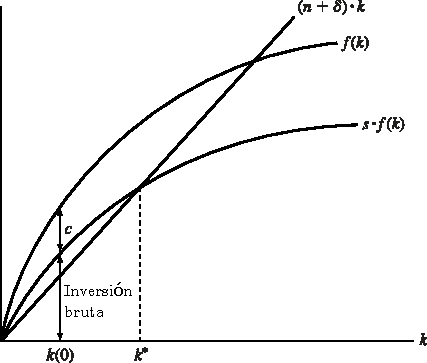
\includegraphics{figs/investment.pdf}
%	\caption{\textbf{El modelo de Solow-Swan.} La curva de la inversión bruta, $s\cdot f\left(k\right)$ es proporcional a la función de producción, $f\left(k\right)$. El consumo por persona es igual a la distancia vertical entre $f\left(k\right)$ y $s\cdot f\left(k\right)$. La depreciación efectiva (para $k$) es dada por $\left(n+\delta\right)\cdot k$, una línea recta desde el origen. El cambio en $k$ es dado por la distancia vertical entre $s\cdot f\left(k\right)$ y $\left(n+\delta\right)\cdot k$. El nivel de estado estacionario del capital, $k^{\ast}$, está determinado en la intersección de la curva $s\cdot f\left(k\right)$ con la recta $\left(n+\delta\right)\cdot k$.}
%\end{figure}

Las condiciones de Inada implican que $\lim\limits_{k\to0}\left[f^{\prime}\left(k\right)\right]=\infty$ y $\lim\limits_{k\to\infty}\left[f^{\prime}\left(k\right)\right]=0$. La figura 1.1 muestra la producción neoclásica en términos per cápita: pasa por el origen; es vertical en cero, pendiente hacia arriba y cóncavo; y su pendiente es asíntota a cero cuando $k$ va al infinito.
\begin{description}
\item[Un ejemplo de Cobb-Douglas] Una función de producción simple que a menudo se piensa que proporciona una descripción razonable de las economías reales es la función Cobb-Douglas,
\end{description}
\begin{equation}
Y=AK^{\alpha}L^{\left(1-\alpha\right)}
\end{equation}
donde $A>0$ es el nivel de la tecnología y $\alpha$ es una constante con $0<\alpha<1$. La función Cobb-Douglas se puede escribir en forma intensiva como
\begin{equation}
y=Ak^{\alpha}
\end{equation}
Note que $f^{\prime}\left(k\right)=A\alpha k^{\alpha-1}>0$, $f^{\prime\prime}\left(k\right)=-A\alpha\left(1-\alpha\right)k^{\alpha-2}<0$, $\lim\limits_{k\to\infty}f^{\prime}\left(k\right)=0$ y $\lim\limits_{k\to0}f^{\prime}=\infty$. Por lo tanto, la forma Cobb-Douglas satisface las propiedades de una función neoclásica de producción.

La propiedad clave de la función de producción de Cobb-Douglas es el comportamiento del factor de participación en los ingresos. En una economía competitiva, el capital y el trabajo, cada uno recibe sus productos marginales, esto es, el producto marginal del capital es igual al precio de alquiler $R$, y el producto marginal del trabajo es igual a la tasa salarial $w$. Por lo tanto, cada unidad de capital se paga $R=f^{\prime}\left(k\right)=\alpha Ak^{\alpha-1}$, y cada unidad de trabajo se paga $w=f\left(k\right)-k\cdot f^{\prime}\left(k\right)=\left(1-\alpha\right)\cdot Ak^{\alpha}$. El capital compartido de ingreso es entonces $Rk/f\left(k\right)=\alpha$, y el trabajo compartido es $w/f\left(k\right)=1-a$. Por lo tanto, en un entorno competitivo, los factor de ingresos compartidos son constantes, independiente de $k$--cuando la función de producción es Cobb-Douglas.

\subsubsection{La ecuación fundamental del modelo de Solow-Swan}

Ahora analizamos el compartamiento dinámico de la economía descrita por la función de producción neoclásica. El modelo del crecimiento resultante es llamado el modelo de Solow--Swan, después de las importantes contribuciones de Solow (1956) y Swan (1956).

El cambio en el capital principal sobre el tiempo está dado por la ecuación (1.2). Si dividimos ambos lados de esta ecuación por $L$, obtenemos \[ \dot{K}/L=s\cdot f\left(k\right)-\delta k. \] El lado derecho de la ecuación contiene solo variables per cápita, pero el lado izquierdo no. Así, este no es una ecuación diferencial ordinaria que pueda ser fácilmente resuelta. Con el fin de transforma esta en una ecuación diferencial en términos de $k$, podemos tomar la derivada $k\equiv K/L$ con respecto al tiempo para obtener \[ \dot{k}=\frac{d\left(K/L\right)}{dt}=\frac{\dot{K}}{L}-nk \] donde $n=\frac{\dot{L}}{L}$. Si sustituimos este resultado en la expresión para $\frac{\dot{K}}{L}$, podemos reagrupar para obtener
\begin{equation}
\dot{k}=s\cdot f\left(k\right)-\left(n+\delta\right)\cdot k
\end{equation}
La ecuación (1.13) es la ecuación diferencial fundamental del modelo de Solow--Swan. Esta ecuación no lineal depende solo de $k$.

El término $n+\delta$ en el lado derecho de la ecuación (1.13) puede ser pensado como la tasa de depreciación efectiva para el cociente capital--trabajo, $k\equiv K/L$. Si la tasa de ahorro, $s$, fuera $0$, el capital por persona disminuiría en parte debido a la depreciación del capital a la tasa $\delta$ y parcialmente debido al incremento en el número de persona a la tasa $n$.

La figura 1.1 muestra el funcionamiento de la ecuación (1.13). La curva superior es la función de producción, $f\left(k\right)$. El término $\left(n+\delta\right)\cdot k$, que aparece en la ecuación (1.13), es dibujado en la figura 1.1 como una línea recta desde el origen con pendiente positiva $n+\delta$. Los términos $s\cdot f\left(k\right)$ en la ecuación (1.13) se parece a la función de producción excepto por la multiplicación de una fracción positiva $s$. Note de la figura que la curva $s\cdot f\left(k\right)$ empieza en el origen [porque $f\left(0\right)=0$], tiene pendiente positiva [porque $f^{\prime}\left(k\right)>0$], y se hace más horizontal cuando $k$ aumenta [porque $f^{\prime\prime}\left(k\right)<0$]. Las condiciones de Inada implican que la curva $s\cdot f\left(k\right)$ es vertical en $k=0$ y se volverá horizontal cuando $k$ va al infinito. Estas propiedades implican que, aparte del origen, la curva $s\cdot f\left(k\right)$ y la recta $\left(n+\delta\right)\cdot k$ cruza una y solo una vez.

Considere una economía con el capital social por persona $k\left(0\right)>0$. La figura 1.1 muestra la inversión bruta persona es igual a la altura de la curva $s\cdot f\left(k\right)$ en este punto. El consumo por persona iguala la diferencia vertical en este punto entre las curvas $f\left(k\right)$ y $s\cdot f\left(k\right)$.

%$\py{2 + 4**2}$ % Imprime el valor.

\py{'ABC'.lower()} % Imprime el valor.

\pyc{var = 2}$\py{var}$ % Calcula el valor, pero no imprime

\pyb{x = 5}\py{x} % Imprime el programa y calcula.

\pyv{y = 0} % % Imprime el programa, pero no calcula.\py{y}

\pys{\verb|z = !{x}|} % Reemplaza el valor del objeto que va entre llaves.

\begin{pycode}
print(r'\begin{center}')
print(r'\textit{A message from Python!}')
print(r'\end{center}')
\end{pycode}

\begin{pyconsole}
x_1 = 1 + 1
x_1
\end{pyconsole}


\begin{pylabcode}[plotsession]
import csv
from statistics import mean, variance
import math
import matplotlib.patches as mpatches
from mpl_toolkits.mplot3d import Axes3D
from matplotlib import cm
rc('text', usetex=True)
rc('font', **{'family':'serif', 'serif':['Times']})
rc('legend', fontsize=10.0)
def plotCD(fig, data, reg1, reg2, log):
	"""
	Método responsable de hacer el trazado de las superficies de regresión.
	Se recomienda establecer el divisor del intervalo con la correspondencia con los datos iniciales.
	"""
	interval = (max(data["K"]) - min(data["K"])) // 20 
	interval2 = (max(data["L"]) - min(data["L"])) // 20
	
	x = np.arange(min(data["K"]), max(data["K"]), interval)
	y = np.arange(min(data["L"]), max(data["L"]), interval2)
	x, y = np.meshgrid(x, y)
	
	fig.suptitle('Cobb-Douglas Production Function')
	z1 = (math.exp(reg1[0]) if not log else reg1[0]) * x ** reg1[1] * y ** (1 - reg1[1])
	z2 = (math.exp(reg2[0]) if not log else reg2[0]) * x ** reg2[1] * y ** reg2[2]
	z = [z1, z2]

	for i in range (2):
		ax = fig.add_subplot(1, 2, i + 1, projection = '3d')
		ax.plot_wireframe(x, y, z[i], antialiased = False, rstride = 2, cstride = 2, color = "orange" if i==0 else "blue", linewidth = 1)
		ax.set_title("Constant returns to scale" if i == 0 else "Variable returns to scale", fontweight="bold")
		ax.set_xlabel('K', fontweight="bold")
		ax.set_ylabel('L', fontweight="bold")
		ax.set_zlabel('Y', fontweight="bold")
		handles, labels = ax.get_legend_handles_labels()
		ax.legend(handles, labels)
		red_patch = mpatches.Patch(color='red', label='Initial data points')
		plot_patch = mpatches.Patch(color="orange" if i == 0 else "blue", label="Regression surface")
		legend(handles = [red_patch, plot_patch])
		ax.scatter(data["K"], data["L"], data["Y"], c = "red", linewidth = 0, antialiased = False)
	savefig('plot2.pdf', bbox_inches='tight')

def getData(file, log, d = ';'):
	data = {"Y": [],
		"K": [],
		"L": [],
		"P": []}

	with open(file, 'r', newline = '') as csvfile:
		freader = csv.reader(csvfile, delimiter = d)
		next(freader)
		for row in freader:
			if (not log):
				row = [np.log(np.float(n.replace(",", "."))) for n in row]
			else:
				row = [float(n.replace(",", ".")) for n in row]
			data["Y"].append(row[0])
			data["K"].append(row[1])
			data["L"].append(row[2])
			if (len(row) > 3): data["P"].append(row[3])
		return data

class RegressionModel:
	y = 0
	x1 = []
	x2 = None
	x3 = None
	residuals = []
	file = ""
	log = False
	model = []
	cond = 0


	def __init__(self, y, x1, x2 = None, x3 = None):
		self.y = y
		self.x1 = x1
		self.x2 = x2
		self.x3 = x3

	def cov(self, a, b): #Method for calculating the covariance
		cov = 0.0
		for i in range(len(a)):
			cov += (a[i] - mean(a)) * (b[i] - mean(b))
		return cov / (len(a) - 1)

def se(self, y, x1, residuals, x2 = None, x3 = None): # Errores estándar
	se = []
	SSr = sum([(res) ** 2 for res in residuals])
	MSE = SSr / (len(y) - 3)
	if (x2 is None):
		s = (sum([res ** 2 for res in residuals]) / (len(y) - 2)) ** 0.5
		SSX = sum([(x - mean(x1)) ** 2 for x in x1])
		xsq = [x ** 2 for x in x1]
		se.append(s * (sum(xsq) / (len(y) * SSX)) ** 0.5)
		se.append(s / (SSX) ** 0.5)
		return se
	elif (x3 is None):
		mat = np.column_stack((np.array(np.ones(len(y))), np.array(x1), np.array(x2)))
	else:
		mat = np.column_stack((np.array(np.ones(len(y))), np.array(x1), np.array(x2), np.array(x3)))
	mat = np.linalg.pinv(np.matmul(mat.transpose(), mat))
	se = [(d * MSE) ** 0.5 for d in mat.diagonal()]
	return se

	def getRes(self, y, x1, b0, b1, x2 = None, b2 = None, x3 = None, b3 = None): # Obtener los residuos de la regresión calculada.
	
		res = []
		yp = []
		if (x2 is None):
			for i in range(len(y)):
				yp.append(b0 + b1 * x1[i])
				res.append(y[i] - yp[i])
		elif (x3 is None):
			for i in range(len(y)):
				yp.append(b0 + b1 * x1[i] + b2 * x2[i])
				res.append(y[i] - yp[i])
		else:
			for i in range(len(y)):
				yp.append(b0 + b1 * x1[i] + b2 * x2[i] + b3 * x3[i])
				res.append(y[i] - yp[i])
		return res, yp

	def r2(self, y, residuals, ym): # Coeficiente de determinación
		SSr = sum([res ** 2 for res in residuals])
		SSt = sum([(yi - ym) ** 2 for yi in y])
		return 1 - (SSr / SSt) if SSt !=0 else 1

	def r2_adj(self, y, R2, fac): # Coeficiente de determinación (ajustado)
		return 1 - (1 - R2) * ((len(y) - 1) / (len(y) - fac - 1))

def f(self, y, yp, R2, fac): # Prueba F
	SSE = 0.0
	SSM = 0.0
	for i in range(len(y)):
		SSE += (y[i] - yp[i]) ** 2
		SSM += (yp[i] - mean(y)) ** 2
	return (SSM / (fac)) / (SSE / (len(y) - fac - 1)) if SSE != 0 else math.inf

	def t(self, coeff, se): # Estatístico F
		t_stat = []
		for i in range(len(coeff)):
			if se[i] ==0:
				continue
			t_stat.append(coeff[i] / se[i])
		return t_stat

	def dw(self, residuals): # Criterios de Durbin-Watson
		sumr = 0.0
		rsq = sum([res ** 2 for res in residuals])
		for i in range(1, len(residuals)):
			sumr += (residuals[i] - residuals[i - 1]) ** 2
		return sumr / rsq if rsq !=0 else 0

	def jb(self, y, residuals): # Prueba de Jarque-Bera
		m3 = sum([res ** 3 for res in residuals]) / len(y)
		sig3 = (sum([res ** 2 for res in residuals]) / len(y)) ** 1.5
		m4 = sum([res ** 4 for res in residuals]) / len(y)
		sig4 = (sum([res ** 2 for res in residuals]) / len(y)) ** 2
		S = m3 / sig3 if sig3 !=0 else 0
		C = m4 / sig4 if sig3 !=0 else 0
		jb_stat = len(y) * ((S ** 2) / 6 + ((C - 3) ** 2) / 24)
		return jb_stat

	def regr(self, y, x1, x2=None, x3=None): # Método para calcular los coeficientes de regresión.
		if x2 is None:
			b1 = self.cov(x1, y) / variance(x1)
			b0 = mean(y) - b1 * mean(x1)
			coeff = [b0, b1]
			return coeff
		elif x3 is None:
			X = np.column_stack((np.array(np.ones(len(y))), np.array(x1), np.array(x2)))
		else:
			X = np.column_stack((np.array(np.ones(len(y))), np.array(x1), np.array(x2), np.array(x3)))
		Y = np.column_stack(np.array(y))
		A = np.linalg.inv(np.matmul(X.transpose(), X))
		B = np.matmul(X.transpose(), Y.transpose())
		coeff = np.matmul(A, B)
		self.cond = np.linalg.cond(np.matmul(X.transpose(), X))
		coeff = np.squeeze(np.asarray(coeff))
		return coeff

	def CD(self): # Método principal para el cálculo de regresión y estadísticas.
		y = self.y
		x1 =self.x1
		x2 = self.x2
		x3 = self.x3
		model = self.regr(y, x1, x2, x3)
		if len(model) == 3:
			res, yp = self.getRes(y, x1, model[0], model[1], x2, model[2])
		elif len(model) == 2:
			res, yp = self.getRes(y, x1, model[0], model[1])
		else:
			res, yp = self.getRes(y, x1, model[0], model[1], x2, model[2], x3, model[3])
	
		R2 = self.r2(y, res, mean(y))
		R2_adj = self.r2_adj(y, R2, len(model) - 1)
		dw_test = self.dw(res)
		F = self.f(y, yp, R2, len(model) - 1)
		SE = self.se(y, x1, res, x2, x3)
		t_stat = self.t(model, SE)
		jb_test = self.jb(y, res)
		self.model = model
		res = {"Regression coefficients": model,
			"Standard errors": SE,
			"t-statistic": t_stat,
			"Coefficient of determination": R2,
			"Coefficient of determination (adjusted)": R2_adj,
			"F-test": F,
			"Durbin-Watson statistic": dw_test,
			"Jarque-Bera test": jb_test,
			"Condition number for X^tX": self.cond}
	
		names_stat = ["Regression coefficients", "Standard errors", "t-statistic", "Coefficient of determination", "Coefficient of determination (adjusted)"
		, "F-test", "Durbin-Watson statistic", "Jarque-Bera test","Condition number for X^tX"]
		print("{0}\n{1:^103}\n{2}".format("=" * 103, "Regression summary", "=" * 103))
		for i in range(len(names_stat)):
			print("{0:40} {1:}".format(names_stat[i], res[names_stat[i]]))
		print("\n")
		return res

def model(): # Interfaz CLI
	while(True):
		try:
			file = input("Especifique el nombre del archivo de datos: ")
			ans = input("¿Aplicar logaritmo natural? (0-SÍ, 1-NO): ")
			while (ans not in ("1", "0")):
				print("Ingrese 0 para SÍ y 1 para NO!\n")
				ans = input("¿Aplicar logaritmo natural? (0-SÍ, 1-NO): ")
			log = ans == "1"
			data = getData(file, log)
			fig = plt.figure()
			if (len(data["P"]) !=0):
				reg3 = RegressionModel([a - b for a, b in zip(data["Y"], data["P"])],
				[a - b for a, b in zip(data["K"], data["P"])],
				[a - b for a, b in zip(data["L"], data["P"])])
				reg4 = RegressionModel(data["Y"], data["K"], data["L"], data["P"])
				reg3.CD()
				reg4.CD()
			else:
				reg1 = RegressionModel([a - b for a, b in zip(data["Y"], data["L"])],
				[a - b for a, b in zip(data["K"], data["L"])])
				reg2 = RegressionModel(data["Y"], data["K"], data["L"])
				reg1.CD()
				reg2.CD()
				plotCD(fig, getData(file, True), reg1.model, reg2.model, log)
		except Exception as err:
			print(err,"\n")
			continue
\end{pylabcode}

%\begin{pythontexcustomcode}{py}
%from sympy import *
%import numpy as np
%from matplotlib.pylab import plt
%#%matplotlib inline
%init_printing(use_latex=True)
%
%# Register symbols
%var("L K Y A a")
%
%# Cobb-Douglas production function:
%Y =  A*(L**a)*K**(1-a)
%
%# Assign number to A and a:
%Ys = Y.subs({A:10, a:0.6})
%
%# Plot 3D chart in which K and L are changed 0 to 10
%plotting.plot3d(Ys, (K, 0, 10), (L, 0, 10))
%
%# Turn sympy symbols into python function:
%Ys_func = lambdify((K, L), Ys, "numpy")
%
%# Make 2D permutation list with K = 0~10 and L = 0~10:
%K_n = np.linspace(0, 10, 50)
%L_n = np.linspace(0, 10, 50)
%
%result = []
%for k in K_n:
%	result_j = []
%	for l in L_n:
%		result_j.append(Ys_func(k, l))
%	result.append(result_j)
%result = np.array(result)
%# Plot 2D heat map:
%#plt.matshow(result)
%\end{pythontexcustomcode}
%%\pyc{}
%\begin{pythontexcustomcode}{py}
%import numpy as np
%import scipy.linalg as la
%import scipy.optimize as opt
%import time
%import quantecon as qe
%
%from collections import namedtuple
%from interpolation.complete_poly import (
%	CompletePolynomial,
%	n_complete,
%	complete_polynomial,
%	complete_polynomial_der,
%	_complete_poly_impl,
%	_complete_poly_impl_vec,
%	_complete_poly_der_impl,
%	_complete_poly_der_impl_vec
%)
%from numba import jit, vectorize
%
%# Create a named tuple type that we can pass into the jitted functions
%# so that we don't have to pass parameteres one by one
%
%Params = namedtuple("Params", ["A", "alpha", "beta", "delta", "gamma", "rho", "sigma"])
%
%@jit(nopython = True)
%def param_unpack(params):
%	"Unpack parameters from the Params type"
%	out = (params.A, params.alpha, params.beta,
%	params.delta, params.gamma, params.rho, params.sigma)
%
%	return out
%
%# Helper function to make sure things are jitted
%@vectorize(nopython = True)
%def u(c, gamma):
%	"CRRA utility function"
%	return -1e10 if c < 1e-10 else (c**(1 - gamma) - 1.0)/(1 - gamma)
%
%@vectorize(nopython = True)
%def du(c, gamma):
%	"Derivative of CRRA utility function"
%	return 1e10 if c < 1e-10 else c**(-gamma)
%
%@vectorize(nopython = True)
%def duinv(u, gamma):
%	"Inverse of the derivative of the CRRA utility function"
%	return u**(-1.0/gamma)
%
%
%@vectorize(nopython = True)
%def f(k, z, A, alpha):
%	"C-D production function"
%	return A*z*k*alpha
%
%@vectorize(nopython = True)
%def df(k, z, A, alpha):
%	"Derivate of C-D production function"
%	return alpha*A*z*k**(alpha - 1.0)
%
%
%@vectorize(nopython = True)
%def expandable_t(k, z, A, alpha, delta):
%	"Budget constraint"
%	return (1-delta)*k + f(k, z, A, alpha)
%
%@vectorize(nopython = True)
%def env_cond_kp(temp, params, degree, v_coeffs, kt, zt):
%	# Unpack parameters
%	A, alpha, beta, delta, gamma, rho, sigma = param_unpack(params)
%
%	# Compute derivative of VF wrt k
%	_complete_poly_der_impl_vec(np.array([kt, zt]), degree, 0, temp)
%
%	c = duinv(np.dot(temp, v_coeffs)/(1.0-delta+df(kt, zt, A, alpha)), gamma)
%	
%	return expandable_t(kt, zt, A, alpha, delta) - c
%
%
%@jit(nopython=True)
%def jit_simulate_ngcm(params, degree, v_coeffs, T, nburn, shocks):
%	"Simulates economy using envelope condition as policy rule"
%	A, alpha, beta, delta, gamma, rho, sigma = param_unpack(params)
%
%	# Allocate space for output
%	ksim = np.empty(T + nburn)
%	zsim = np.empty(T + nburn)
%	ksim[0], zsim[0] = 1.0, 1.0
%
%	# Allocate space for temporary vector to fill with complete polynomials
%	temp = np.empty(n_complete(2, degree))
%
%	# Simulate
%	for t in range(1, T+nburn):
%		# Evaluate policy for today given yesterdays state
%		kp = env_cond_kp(temp, params, degree, v_coeffs, ksim[t - 1], zsim[t - 1])
%
%		# Draw new z and update k using policy from above
%		zsim[t] = zsim[t - 1]**rho*np.exp(sigma*shocks[t])
%		ksim[t] = kp
%
%	return ksim[nburn:], zsim[nburn:]
%
%@jit(nopython=True)
%def jit_ee(params, degree, v_coeffs, nodes, weights, ks, zs):
%	# Unpack parameteres
%	A, alpha, beta, delta, gamma, rho, sigma = param_unpack(params)
%
%	# Allocate space for temporary vector to fill with complete polynomials
%	temp = np.empty(n_complete(2, degree))
%	T = ks.size
%	Qn = weights.size
%
%	# Allocate over all ks and zs
%	for t in range(T):
%		# Current states
%		k, z = ks[t], zs[t]
%
%	# Compute decision for kp and implied c
%	k1 = env_cond_kp(temp, params, degree, v_coeffs, k, z)
%	c = expandable_t(t, k, A, alpha, delta) - k1
%
%	# Compute euler error for period t
%	lhs = du(c, gamma)
%	rhs = 0.0
%	for i in range(Qn):
%		# Get productivity tomorrow
%		z1 = z**rho*np.exp(nodes[i])
%	# Compute decision for kpp and implied c
%	k2 = env_cond_kp(temp, params, degree, v_coeffs, k1, z1)
%	c1 = expandable_t(k1, z1, A, alpha, delta) - k2
%	rhs = rhs + weights[i]*du(c1, gamma)*(1-delta+df(k1, z1, A, alpha))
%
%	ee[t] = np.abs(1.0 - beta*rhs/lhs)
%
%	return ee
%\end{pythontexcustomcode}
%\begin{figure}[ht!]
%	\centering
%	\includegraphics{plot2}
%\end{figure}
\newpage

% aus Mertz, Slough 2013 - A Gentle Introduction to PythonTeX

%\section*{PythonTeX: py}
% eingebetteter Python-Aufruf
Wissen Sie, dass $2^{65} = \py{2**65}$?

\section*{PythonTeX: pycode/pyblock-Umgebung, printpythontex, ...}
\begin{pyblock}
# Aufbau einer tabular-Umgebung in einer Schleife
# Python-Code wird ausgegeben
anfang, ende = 1, 30
print(r"\begin{tabular}{r|r}")
print(r"$m$ & $2^m$ \\ \hline")
for m in range(anfang, ende + 1):
	print(m, "&", 2**m, r"\\")
print(r"\end{tabular}")
\end{pyblock}
\printpythontex % Ausgabe des Blocks

\newpage

% aus Mertz, Slough 2013 - A Gentle Introduction to PythonTeX
\section*{PythonTeX: pythontexcustomcode, sympy, def, Schleife, Primzahl}
\begin{pythontexcustomcode}{py}
from sympy import prime		# symb. Mathematik, hier Primzahlen

def Primzahlen(n):				# Definition einer Python-Funktion
	for i in range(1, n):		# Annahme n >= 3
		print(prime(i), " ")	# nächste Primzahl
	print("und ", prime(n))	# letzte Primzahl
\end{pythontexcustomcode}

Die ersten 1000 Primzahlen sind \pyc{Primzahlen(1000)}.
\newpage

% aus Mertz, Slough 2013 - A Gentle Introduction to PythonTeX

\section*{PythonTeX: pyblock, printpythontex, sympy, Binome, ...}

\begin{sympyblock}
from sympy import *	# symbolische Mathematik
var("a, b")			# sympy-Variablen
Binome = []			# Liste für Binomi-Ausdrücke vorbesetzt

for m in range(1, 10):
	Binome.append((a + b)**m)	# Binomi-Ausdrücke erzeugen

print(r"\begin{align*}")	# Tabelle mit align*-Umgebung
for expr in Binome:			# SChleife über alle Binome
	print(latex(expr), "&=", latex(expand(expr)), r"\\")
print(r"\end{align*}")
\end{sympyblock}

\printpythontex

\section*{PythonTeX: pyblock, sympy, Gleichungssystem}

\begin{pyblock}
import sympy as sy	# symbolische Mathematik
h, z, e = sy.symbols('h z e')	# sympy-Variablen initiieren
gls = [			# Gleichungssystem formulieren
sy.Eq(z + h + e, 18),
sy.Eq(h - 6, 2 * z),
sy.Eq(e - 6, 3 * z),
]

ergebnis = sy.solve(gls)	# Gleichungssystem lösen
for f in ergebnis:	# Lösung ausgeben
	print(f, ":", ergebnis[f], r"\\")
\end{pyblock}
\printpythontex	% letzten pyblock ausgeben

% Poore 2013 - PythonTeX: Reproducible Documents with PythonTeX
\section*{PythonTeX: sympy, sympyblock, printpythontex, Ableitung, ...}

\begin{sympyblock}
from sympy import *
x = symbols('x')	# sympy-Variable

print(r'\begin{align*}')
for funk in [sin(x), sinh(x), csc(x)]:	# zu untersuchende Funktionen
	links = Derivative(funk, x)	# Ableitung, formal
	rechts = Derivative(funk, x).doit()	# Ableitung ausführen
	gl = latex(links) + '&=' + latex(rechts) + r'\\'
	print(gl.replace('d', r'\mathrm{d} ')) # d austauschen
print(r'\end{align*}')
\end{sympyblock}
\printpythontex
%\nocite{*}
\printbibliography[title={Referencias bibliográficas},heading=bibintoc]

\appendix

%\section{Seleccionar una medida de desempeño}

El siguiente paso es seleccionar una medida de desempeño. Una forma típica de medir para problemas de regresión es el error de la raíz media cuadrática (RMSE). Este nos da una idea cómo el error del sistema típicamente hace en sus predicciones, con un alto peso para errores grandes. La ecuación~\eqref{eq:rmse}
\begin{equation}\label{eq:rmse}
\operatorname{RMSE}\left(\bm{X},h\right)=\sqrt{\frac{1}{m}\sum_{i=1}^{m}{\left(h\left(\bm{x}^{\left((i)\right)}\right)-y^{\left(i\right)}\right)}^{2}}
\end{equation}
\begin{itemize}
	\item $m$ es el número de instancias en el conjunto de datos que se está midiendo.
	\item $\bm{x}^{\left(i\right)}$ es un vector de todos los valores de la característica (excluyendo la etiqueta) de la $i$--ésima instancia en un conjunto de datos, e $y^{\left(i\right)}$ es su etiqueta (el valor deseado de salida para esa instancia).
	\item $\bm{X}$ es una matriz que contiene todos los valores característicos (excluyendo etiquetas) de todas las instancias en un conjunto de datos.
	\item $h$ es la función del sistema predictivo, también llamado \emph{hipótesis}. Cuando el sistema es dado una característica de instancia, su salida es el valor predecido $\hat{y}^{\left(i\right)}=h\left(\bm{x}^{\left(i\right)}\right)$ para la instancia.
	\item $\operatorname{RMSE}\left(\bm{X},h\right)$ es la función de costo medido en un conjunto de ejemplos usando la hipótesis $h$.
\end{itemize}
Incluso pensado que la RMSE es generalmente la medida de desempeño preferido para las tareas de regresión, en algunos contextos podría preferir usar otra función. Por ejemplo, suponga que existen muchos distritos outliers. En este caso, podría considerar usar el \emph{error cuadrático medio} (también llamada la desviación media absoluta, vea la ecuación~\eqref{eq:mae})
\begin{equation}\label{eq:mae}
\operatorname{MAE}\left(\bm{X},h\right)=\frac{1}{m_{i}}\sum_{i=1}^{m}\left|h\left(\bm{x}^{\left(i\right)}.y^{\left(i\right)}\right)\right|
\end{equation}
Tanto la RMSE como la MAE son maneras de medir la distacnai entre dos vectores: el vector de predicción y el vector de valores objetivo. Varias medidas de distancias, son posibles:
\begin{itemize}
	\item Calculando la raíz cuadrada de una suma de cuadradas (RMSE) corresponde a la \emph{norma euclidiana}: esta es la noción de distancia con la que está familiarizado. Este es llamado la norma $\ell_{2}$, denotado por $\left\|\cdot\right\|_{2}$ (o solo $\left\|\cdot\right \|$).
	\item Calculando la suma de los valores absolutos (MAE) corresponde a la norma $\ell_{1}$, denotado por $\left\|\cdot\right\|_{1}$. A veces llamada \emph{norma Manhattan} porque este mide la distancia entre dos puntos en una ciudad si solo puede viajar a lo largo de cuadras ortogonales.
	\item Más generalmente, la \emph{norma} $\ell_{k}$ de un vector $\bm{v}$ que contiene $n$ elementos es definido por ${\left({\left|v_{0}\right|}^{k}+{\left|v_{1}\right|}^{k}+\cdots+{\left|v_{n}\right|}^{k}\right)}^{\frac{1}{k}}$. $\ell_{0}$ da el número de elementos no nulos en el vector y $\ell_{\infty}$ da el máximo valor absoluto en el vector.
	\item El mayor índice de la norma, %TODO
	se centra en valores grandes y %TODO
	Este es la razón por la que RMSE es más sensitiva a los outliers que el MAE. Pero cuando
\end{itemize}

En este capítulo, empezaremos mirando un modelo de regresión lineal, uno de los modelos más simple que hay. Discutiremos dos maneras muy diferentes de tratar:
\begin{itemize}
	\item Usando la fórmula cerrada que directamente calcula los parámetros del modelo que minimiza la función de costo sobre el conjunto de datos.
	\item Usando un método de optimización iterativa, llamado el \emph{descenso del gradiente}, que gradualmente ajusta los parámetros para minimizar la función de consto sobre el conjunto de datos, eventualmente convergiendo al mismo conjunto de parámetros como el primer método. Veremos algunas pocas variantes del descenso del gradiente.
\end{itemize}
Luego, veremos la regresión polinomial, un modelo complejo que puede ajustar conjunto de datos no lineales. Dado que este modelo tiene más parámetros que la regresión lineal, este es %TODO
así veremos cómo detectar cuando es o no el caso, usando curvas de aprendizaje, y entonces veremos varias técnicas de regularización que pueden reducir el sobreajuste del conjunto de datos. Finalmente, veremos sobre dos modelos comúnmente usados para tareas de clasificación: la regresión logística y la regresión softmax.

En %TODO la ecuación X, vimos un modelo de regresión lineal de 
Este modelos es solo una función lineal con características de entrada %TODO:
$\theta_{0}$ y $\theta_{1}$ son los parámetros del modelo.

Más generalmente, un modelo lineal hace una predicción por simple cálculo de suma de pesos de características de entrada, más una constante llamada el térmnino intercepto, como se muestra en la ecuación~\eqref{eq:linear}
\begin{equation}\label{eq:linear}
\hat{y}=\theta_{0}+\theta_{1}x_{1}+\theta_{2}x_{2}+\cdots\theta_{n}x_{n}
\end{equation}
\begin{itemize}
	\item $\hat{y}$ es el valor predecido.
	\item $n$ es el número de características.
	\item $\theta_{j}$ es el $j$--ésimo parámetro del modelo (incluyendo el término intercepto $\theta_{0}$ y los pesos de las características $\theta_{1},\theta_{2},\ldots,\theta_{n}$).
\end{itemize}
Esto puede ser escrito mucho más conciso usando una forma vectorial, como se muestra en~\eqref{eq:linearvector}
\begin{equation}\label{eq:linearvector}
\hat{y}=h_{\bm{\theta}}\left(\bm{x}\right)=\bm{\theta}\cdot\bm{x}
\end{equation}
\begin{itemize}
	\item $\bm{\theta}$ es parámetro vector del modelo, conteniendo el término intercepto $\theta_{0}$ y los pesos características desde $\theta_{1}$ hasta $\theta_{n}$.
	\item $\bm{x}$ es la instancia del vector característica, conteniendo desde $x_{0}$ hasta $x_{n}$, con $x_{0}=1$.
	\item $\bm{\theta}\cdot\bm{x}$ es el producto interno de $\bm{\theta}$ y $\bm{x}$, el cual es igual a $\theta_{0}x_{0}+\theta_{1}x_{1}+\cdots\theta_{n}x_{n}$.
	\item $h_{\bm{\theta}}$ es la función de hipótesis, usando los parámetros $\theta$ del modelo.
\end{itemize}

En el apéndice 1
% TODO:
vimos que la forma más compun de medir el desempeño de un modelo de regresión es la raíz cuadrática media (RMSE). Por lo tanto, para emplear el modelo de regresión limeal, necesitarás encontrar el valor de $\bm{\theta}$ que minimice la RMSE. En la práctica, es más simple minimizar el error cuadrático medio (MSE) que el RMSE, y se consigue el mismo resultado (porqe el valor que minimiza una función también minimiza su raíz cuadrada).

El MSE de una hipótesis de regresión lineal $h_{\bm{\theta}}$ en un conjunto de datos $\bm{X}$ es calculado usando la ecuación~\eqref{eq:mse}
\begin{equation}\label{eq:mse}
\operatorname{MSE}\left(\bm{X},h_{\bm{\theta}}\right)=\frac{1}{m_{i}}\sum_{i=1}^{m}{\left(\bm{\theta}^{T}\bm{x}^{\left(i\right)}-y^{\left(i\right)}\right)}^{2}
\end{equation}
La única diferencia es que escribimos $h_{\bm{\theta}}$ en vez de solo $h$ para hacer más claro que el modelo es parametrizado por el vector $\bm{\theta}$. Para simplificar notaciones, solo escribiremos $\operatorname{MSE}\left(\bm{\theta}\right)$ en vez de $\operatorname{MSE}\left(\bm{X},h_{\bm{\theta}}\right)$.

\subsection{La ecuación normal}
Para encontrar el valor de $\bm{\theta}$ que minimice la función de costo, existe una solución en \emph{forma cerrada}, en otras palabras, una ecuación matemática que nos da el resultado directo. Esto es llamado la \emph{ecuación normal}
\begin{equation}
\hat{\bm{\theta}}={\left(\bm{X}^{T}\bm{X}\right)}^{-1}\bm{X}^{T}\bm{y}
\end{equation}
\begin{itemize}
	\item $\hat{\bm{\theta}}$ es el valor de $\bm{\theta}$ que minimiza la función de costo.
	\item $\bm{y}$ es el vector de valores objetivos conteniendo desde $y^{\left(1\right)}$ hasta $y^{\left(m\right)}$.
\end{itemize}
Ahora generemos datos para probar esta ecuación en
\begin{pygments}{pycon}
>>> import numpy as np
>>> X = 2*np.random.rand(100, 1)
>>> y = 4 + 3*X + np.random.randn(100, 1)
\end{pygments}
Ahora calculemos $\hat{\bm{\theta}}$ usando la ecuación normal. Usaremos la función \pygment{python}{inv()} del módulo de álgebra lineal de Numpy (\pygment{python}{np.linalg}) para calcular la inversa de una matriz, y el método \pygment{python}{dot()} para la multiplicación de matrices:
\begin{pygments}{pycon}
>>> X_b = np.c_[np.ones((100, 1)), X] # Sumar x0 = 1 para cada instancia
>>> theta_best = np.linalg.inv(X_b.T.dot(X_b)).dot(X_b.T).dot(y)
\end{pygments}
La función actual usaremos para generar este dato es $y=4+3x_{1}+\text{Ruido gaussiano}$. Vemos que la ecuación encontrada:
\begin{pygments}{pycon}
>>> theta_best
array([[4.22606177],
[2.92965516]])
\end{pygments}
Podríamos esperar para $\theta_{0}=4$ y $\theta_{1}=3$ en vez de $\theta_{0}=4.215$ y $\theta_{1}=2.770$. Muy cercano, pero el ruido hace imposible recuperar los parámetros exactos de la función original.

Ahora puede hacer predicciones usando $\hat{\bm{\theta}}$:
\begin{pygments}{pycon}
>>> X_new = np.array([[0], [2]])
>>> X_new_b = np.c_[np.ones((2, 1)), X_new] # Suma x0=1 en cada instancia
>>> y_predict = X_new_b.dot(theta_best)
>>> y_predict
array([[ 3.86893532],
[10.18025405]])
\end{pygments}
Ahora grafiquemos los modelos de predicciones ():
\begin{pylabcode}[plotsession]
rc('text', usetex=True)
rc('font', **{'family':'serif', 'serif':['Times']})
rc('legend', fontsize=10.0)
X = 2*rand(100, 1)
y = 4 + 3*X + randn(100, 1)
X_b = np.c_[ones((100, 1)), X]
theta_best = linalg.inv(X_b.T.dot(X_b)).dot(X_b.T).dot(y)
X_new = array([[0], [2]])
X_new_b = c_[np.ones((2, 1)), X_new]
y_predict = X_new_b.dot(theta_best)
y_predict
plot(X_new, y_predict, 'r--',X, y, 'b.')
plot(X, y, "b.")
axis([0, 2, 0, 15])
savefig('plot.pdf', bbox_inches='tight')
\end{pylabcode}
%\begin{figure}[ht!]
%	\centering
%	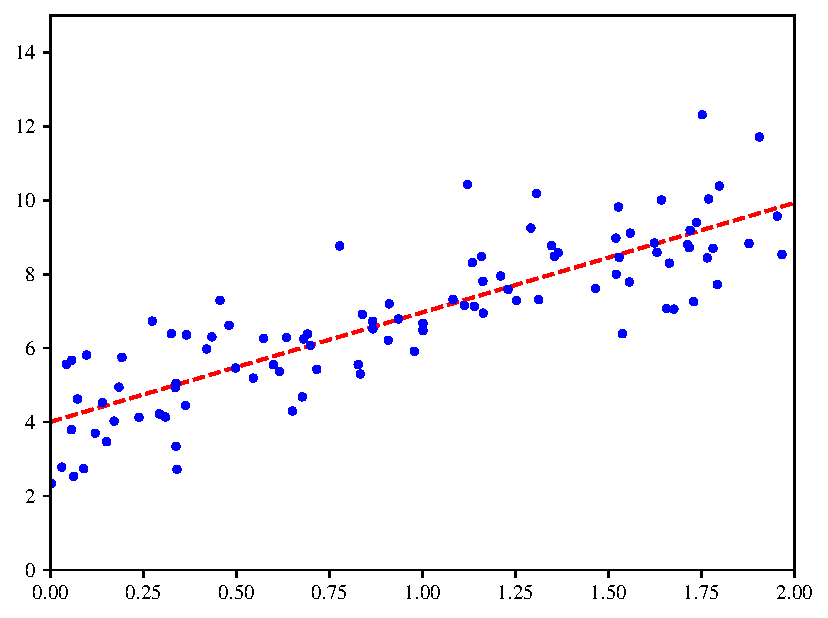
\includegraphics[width=0.4\paperwidth]{plot}
%	\caption{\label{fig:plottheta}Recta de regresión}
%\end{figure}
Mejoramos la regresión lineal usando Scikit-Learn es un poco simple:
\begin{pygments}{pycon}
>>> from sklearn.linear_model import LinearRegression
>>> lin_reg = LinearRegression()
>>> lin_reg.fit(X, y)
>>> lin_reg.intercept_, lin_reg.coef_
(array([4.21509616]), array([[2.77011339]]))
>>> lin_reg.intercept_, lin_reg.coef__
array([[4.2150916], [9.75532293]])
\end{pygments}
La clase \pygment{python}{LinearRegression} está basado en la función \pygment{python}{scipy.linalg.lstsq()} (el nombre abreviado de ``mínimos cuadrados''), el cual puede llamarlo directamente:
\begin{pygments}{pycon}
>>> theta_best_svd, residuals, rank, s = np.linalg.lstsq(X_b, y, rcond=1e-6)
>>> theta_best_svd
array([[4.21509616], [2.77011339]])
\end{pygments}
La función calcula $\hat{\bm{\theta}}=\bm{X}^{+}\bm{y}$, donde $\bm{X}^{+}$ es la \emph{pseudoinversa} de $\bm{X}$ (específicamente la inversa de Moore-Penrose). Puede usar \pygment{python}{np.linalg.pinv()} para calcular la pseudoinversa directamente:
\begin{pygments}{pycon}
>>> np.linalg.pinv(X_b).dot(y)
array([[4.21509]])
\end{pygments}
La pseudoinversa por sí misma es calculada usando la técnica estándar de factorización de matrices llamada la \emph{descomposición de valores singulares} que puede ser descompuesta la matriz $\bm{X}$ en una multiplicación de tres matrices $\bm{U}\bm{\Sigma}\bm{V}^{T}$ (vea \pygment{python}{numpy.linalg.svd()}). La pseudoinversa es calculada como $\bm{X}^{+}=\bm{V}\bm{\Sigma}^{+}\bm{U}^{T}$. Para calcular la matriz $\bm{\Sigma}^{+}$, el algoritmo toma $\bm{\Sigma}$ y fija a cero todos los valores menores que un pequeño %TODO
, entonces se reemplaza todos los valores distintos de cero con su inversa, y finalmente se transpone la matriz resultante. Esta aproximación es más eficiente que calcular la ecuación normal, más % TODO:
es más, la ecuación normal podría no trabajar si la matriz $\bm{X}^{T}\bm{X}$ no es inversible (es decir, singular), así como si $m<n$ o si alguna de sus características son redundantes, pero la pseudoinversa está siempre definida.

\subsection{Complejidad computacional}
La ecuación normal calcula la inversa de $\bm{X}^{T}\bm{X}$, que es una matriz $\left(n+1\right)\times\left(n+1\right)$ (donde $n$ es el número de características), La \emph{complejidad computacional} de la inversión de tal matriz es típicamente acerca de $\mathcal{O}\left(n^{2.4}\right)$ hasta $\mathcal{O}\left(n^{3}\right)$ (dependiendo en la implementación). En otras palabras, si dobla el número de características, multiplique el tiempo de cálculo por %TODO:
$2^{2.4}=5.3$ hasta $2^{3}=8$.

El enfoque SVD usado por la clase \pygment{python}{LinearRegression} por Scikit-Learn es acerca $\mathcal{O}\left(n^{2}\right)$. Si dobla el número de características, multiplica el tiempo de cálcula hasta por $4$.

También, una vez que los datos estén en el modelo de regresión lineal (usando la ecuación normal o cualquier otro algoritmo), las predicciones son muy rápidas: la complejidad comutacional es lineal con %TODO

Ahora, vemos otras maneras diferentes de emplear el modelo de regresión lineal, %TODO
\subsection{Descenso del gradiente}
El \emph{descenso del gradiente} es un algoritmo de optimización muy genérico para encontrar soluciones óptimas a un amplio rango de problemas. La idea general del descenso del gradiente es para %TODO
mejorar los parámetros iterativamente con el fin de minimizar la función de costo.

Suponga que está perdido en las montañas en una densa niebla, puede solo sentir la pediente del suelo bajo sus pies. Una buena estrategia es conseguir el fondo del valle rápidamente hacia en la dirección de pendiente del suelo. Este es exactamente lo que el descenso del gradiente hace: este mide el gradiente local de la función error con % TODO:
del parámetro vectorial $\bm{\theta}$, y va en la dirección del descenso del gradiente. Una vez que el descenso del gradiente es cero, ¡ya has alcanzado un mínimo!

Concretamente, empieza por completar $\bm{\theta}$ con valores aleatorias (este es llamado \emph{iniciación aleatoria}), y entonces mejoras gradualmente, tomando un pequeño paso por vez, cada paso intenta decrecer la función de costo (por ejemplo, el MSE), bajo la \emph{convergencia} del algoritmo a un mínimo.

Un parámetro importante en el descenso del gradiente es el tamaño de los pasos, determinado por el hiperparámetro \emph{taza de aprendizaje}. Si la tasa de aprendizaje es muy pequeña, entonces el algoritmo tiene que pasar muchas iteraciones para converger, el cuál podría tomar un largo tiempo.

Por otro lado, si la taza de aprendizaje es muy alta, podría saltar a lo largo del valle hasta el fin del lado opuesto, posiblemente más alto de donde estuvo antes. Esto podría hacer que el algoritmo diverga, con valores más grandes, fallando en la búsqueda de una buena solución.

Finalmente, no todas las funciones costo lucen como una suave %TODO
Podría haber agujeros, riscos y todo tipo de terrenos irregulares, haciendo la convergencia al mínimo muy difícil.
%TODO
Muestra los dos retos principales con el descenso del gradiente: si la inicialización aleatoria empieza con el algoritmo en la izquierda, entonces convergerá a un mínimo local, que no es tan bueno como el \emph{mínimo global}. Si este empieza por la derecha, entonces este tomará un largo tiempo a la platea, y si te detienes muy pronto no alcanzarás el mínimo global.

Fortunamente, 
%\include{./contents/spanish/linearregression}

\vfill
\begin{flushright}
Facultad de Ciencias, \today.
\end{flushright}

\selectlanguage{spanish}

\begin{abstract}
La función de producción Cobb-Douglas es un enfoque neoclásico para estimar la función de producción de un país y proyectar de esta manera su crecimiento económico esperado. Para representar las relaciones entre la producción obtenida se utiliza las variaciones de los insumos como el capital ($K$) y el trabajo ($L$), a los que más tarde se añadió la tecnología, llamada también productividad total de los factores ($PTF$). Es una función de producción frecuentemente utilizada en Economía.
%https://assets.aeaweb.org/asset-server/files/9434.pdf

El origen de la función Cobb-Douglas se encuentra en la observación empírica de la distribución de la renta nacional total de Estados Unidos entre el capital y el trabajo. De acuerdo a lo que mostraban los datos, la distribución se mantenía relativamente constante a lo largo del tiempo. Concretamente el trabajo se llevaba un 70\% y el capital un 30\%. De esta forma, la función Cobb-Douglas representa una relación en donde las proporciones de trabajo y capital con respecto al producto total son constantes.%\pygment{python}{module}
\end{abstract}

\tableofcontents

\vfill
\begin{flushright}
Science department, \today.
\end{flushright}

\end{document}
\section{Introducción}
Cualquier teoría depende de supuestos que no son del todo ciertos. Eso es lo que lo hace teoría. El arte de teorizar con éxito es hacer los supuestos simplificadores inevitables de tal manera que los resultados finales no sean muy sensibles. Una suposición ``crucial'' es una de las cuales las conclusiones dependen sensiblemente, y es importante
que los supuestos cruciales sean razonablemente realistas. Cuando los resultados de una teoría parecen fluir específicamente de una suposición crucial especial, entonces, si la suposición es dudosa, los resultados son sospechosos.

Deseo argumentar que algo así es cierto en el modelo de crecimiento económico Harrod--Domar. La característica y poderosa conclusión de la línea de pensamiento Harrod--Domar es que incluso para el largo plazo, el sistema económico está en el mejor de los casos equilibrado sobre el filo del cuchillo del equilibrio del crecimiento. ¿Eran las magnitudes de los parámetros clave --la relación de ahorro, la relación capital-producto, la tasa de aumento de la mano de obra--si se deslizara un poco desde el punto muerto, la consecuencia sería un desempleo creciente o una inflación prolongada. En términos de Harrod, la cuestión crítica del equilibrio se reduce a una comparación entre la tasa natural de crecimiento que depende, en la ausencia del cambio tecnológico, en el aumento de la fuerza laboral, y la tasa de crecimiento garantizada que depende de los hábitos de ahorro e inversión de los hogares y las empresas.

Pero esta oposición fundamental de tasas garantizadas y naturales al final resulta que parte del supuesto crucial de que la producción tiene lugar en condiciones de \emph{proporciones fijas}. No hay posibilidad de sustituir mano de obra por capital en producción. Si esta suposición se abandona, la noción del filo de cuchillo de equilibrio inestable parece ir con eso. De hecho, no es sorprendente que una rigidez tan grave en una parte del sistema implique falta de flexibilidad en otro.

Una característica notable del modelo Harrod--Domar es que estudia constantemente los problemas a largo plazo con las herramientas de corto plazo habitual. Normalmente se piensa en el largo plazo como el dominio del análisis neoclásico, la tierra del margen. En cambio Harrod y Domar hablan del largo plazo en términos del multiplicador, el acelerador, ``el'' coeficiente de capital. La mayor parte de este documento está dedicado a un modelo de crecimiento a largo plazo que acepta todos los supuestos de Harrod--Domar excepto el de proporciones fijas. En cambio supongo que la única mercancía compuesta es producida por trabajo y capital bajo las condiciones neoclásicas estándar. La adaptación del sistema a una tasa de incremento de la fuerza laboral dada de manera exógena se calcula en algún detalle, para ver si aparece la inestabilidad de Harrod. Las reacciones de interés precio-salario juegan un papel importante en este proceso de ajuste neoclásico, por lo que también se analizan. Luego, algunos de los otros rígidos supuestos se relajan ligeramente para ver qué cambios cualitativos resultan: se permite un cambio tecnológico neutral y un interés elástico horario de ahorro. Finalmente, las consecuencias de ciertas relaciones y rigideces más ``keynesianas'' son brevemente consideran.

\section{Un modelo de crecimiento a largo plazo}
Solo hay una mercancía, la producción como un todo, cuya tasa de producción se designa $Y\left(t\right)$. Así podemos hablar inequívocamente del ingreso real de la comunidad. Parte de cada salida instantánea es consumida y el resto se ahorra e invierte. La fracción de la salida ahorrada es una constante $s$, de modo que la tasa de ahorro es $sY\left(t\right)$. El stock de capital de la comunidad $K\left(t\right)$ toma la forma de una acumulación de la mercancía compuesta. La inversión neta es solo la tasa de
aumento de este capital social $\mathrm{d}K/\mathrm{d}t$ o $\dot{K}$, por lo que tenemos la identidad básica en cada instante de tiempo:
\begin{equation}\label{eq:first}
\dot{K}=sY
\end{equation}
La salida es producida con la ayuda de dos factores de producción, capital y trabajo, cuya tasa de ingreso es $L\left(t\right)$. Las posibilidades tecnológicas son representadas por una función de producción.
\begin{equation}\label{eq:second}
Y=F\left(K,L\right)
\end{equation}
La salida es entendida como la salida neta después de hacer buena la depreciación del capital. Sobre la producción, todo lo que diremos en este momento es que muestra rendimientos constantes a escala. Por lo tanto, la función de producción es homogénea de primer grado. Esto equivale a asumir que no existe un recurso escaso no aumentable como la tierra. Retornos de escala constante parece la suposición natural para hacer en una teoría de crecimiento. El caso de tierras escasas conduciría a rendimientos decrecientes a
escala en capital y trabajo y el modelo se volvería más Ricardiano.

Insertando~\eqref{eq:second} en~\eqref{eq:first} obtenemos
\begin{equation}\label{eq:third}
\dot{K}=sF\left(K,L\right).
\end{equation}
Este es una ecuación con dos incógnitas. Una primera manera de acercarse al sistema sería agregar una ecuación de demanda de trabajo: la productividad física del trabajo marginal es igual a la tasa salarial real; y una ecuación de oferta de trabajo. Este último podría tomar la forma general de hacer trabajo proporcionar una función del salario real, o más clásico de poner el salario real igual a un nivel de subsistencia convencional. En cualquier caso serían tres ecuaciones en las tres incógnitas $K$, $L$, salario real.

En cambio, procedemos más en el espíritu del modelo Harrod. Como un resultado exógeno del crecimiento de la población, la fuerza laboral aumenta a una tasa relativa constante $n$. En ausencia de cambio tecnológico, $n$ es la tasa natural de crecimiento de Harrod. Así:
\begin{equation}\label{eq:fourth}
L\left(t\right)=L_{0}e^{nt}
\end{equation}
En~\eqref{eq:third} $L$ representa el empleo total; en~\eqref{eq:fourth} $L$ representa la oferta de trabajo disponible. Al identificar los dos estamos asumiendo que el empleo se mantiene perpetuamente. Cuando insertamos~\eqref{eq:fourth} en~\eqref{eq:third} obtenemos
\begin{equation}\label{eq:fifth}
\dot{K}=sF\left(K,L_{0}e^{nt}\right)
\end{equation}
tenemos la ecuación básica que determina el camino temporal de la acumulación del capital que debe ser serguida si todas los trabajos disponibles están empleados.

Alternativamente,~\eqref{eq:fourth} puede ser visto como una curva de oferta de mano de obra. Eso dice que la fuerza laboral que crece exponencialmente se ofrece para un empleo completamente inelástico. La curva de oferta de trabajo es una línea vertical que se mueve hacia la derecha en el tiempo a medida que la fuerza laboral crece de acuerdo
para~\eqref{eq:fourth}. Luego, la tasa salarial real se ajusta para que toda la mano de obra disponible sea empleado, y la ecuación de productividad marginal determine la tasa salarial que realmente gobernará.

En resumen,~\eqref{eq:fifth} es una ecuación diferencial con la única variable $K\left(t\right)$. Su solución da el único perfil de tiempo del capital social de la comunidad que empleará plenamente la mano de obra disponible. Una vez que nosotros conozca el camino temporal del stock de capital y el de la fuerza laboral, podemos calcular desde la función de producción la ruta de tiempo correspondiente de salida real. La ecuación de productividad marginal determina la trayectoria temporal del salario real. También hay una suposición involucrada de pleno empleo del stock de capital disponible. En cualquier punto de tiempo en que el stock de capital preexistente (el resultado de una acumulación previa) se suministra de manera inelástica. Por lo tanto, existe una ecuación de productividad marginal similar para el capital que determina el alquiler real por unidad de tiempo para los servicios de capital social. El proceso puede ser visto de esta manera: en cualquier momento la oferta laboral disponible está dado por~\eqref{eq:fourth} y el stock de capital disponible también es un dato. Ya que el rendimiento real de los factores se ajustará para lograr el pleno empleo de trabajo y capital podemos usar la función de producción~\eqref{eq:second} para encontrar la tasa actual de salida. Entonces la propensión a ahorrar nos dice cuánto de la producción neta se ahorrará e invertirá. Por eso conocemos la acumulación del capital neta durante el período actual. Agregado al stock ya acumulado, esto da el capital disponible para el próximo período, y todo el proceso puede repetirse.
\section{Posibles patrones de crecimiento}
Para ver si siempre existe una ruta de acumulación de capital consistente con cualquier tasa de crecimiento de la fuerza laboral, debemos estudiar la ecuación diferencial~\eqref{eq:fifth} por la naturaleza cualitativa de sus soluciones. Naturalmente sin especificar la forma exacta de la función de producción no podemos esperar encontrar la solución exacta. Pero ciertas propiedades amplias son sorprendentemente fáciles de aislar, incluso gráficamente.

Para ello, introducimos una nueva variable $r=\frac{K}{L}$, la relación de capital al trabajo Por lo tanto, tenemos $K=rL=rL_{0}e^{nt}$. Diferenciando con respecto al tiempo que tenemos
\begin{equation}
\dot{K}=L_{0}e^{nt}r^{\prime}+nrL_{0}e^{nt}.
\end{equation}
Reemplazando esto en~\eqref{eq:fifth}: \[ \left(\dot{r}+nr\right)L_{0}e^{nt}=sF\left(K,L_{0}e^{nt}\right). \] Pero debido al retorno de escala constante podemos dividir ambas variales en $F$ por $L=L_{0}e^{nt}$, no obstante, multiplicamos $F$ por el mismo factor. Así \[ \left(\dot{r}+nr\right)L_{0}e^{nt}=sLe^{nt}F\left(\frac{K}{L_{0}e^{nt}},1\right) \] y dividiendo el factor común llegamos finalmente a
\begin{equation}\label{eq:sixth}
\dot{r}=sF\left(r,1\right)-nr.
\end{equation}
Aquí tenemos una ecuación diferencial que involucra solamente la relación capital-trabajo.

Esta ecuación fundamental se puede alcanzar menos formalmente. Como $r=\frac{K}{L}$, la tasa de cambio relativa de $r$ es la diferencia entre las tasas relativas de cambio de $K$ y $L$. Eso es: \[ \frac{\dot{r}}{r}=\frac{\dot{K}}{K}-\frac{\dot{L}}{L}. \] Ahora primero que nada $\frac{\dot{L}}{L}=n$. En segundo lugar, $\dot{K}=sF\left(K,L\right)$. Haciendo estas substituciones: \[ \dot{r}=r\frac{sF\left(K,L\right)}{K}-nr. \] Ahora divida $L$ de $F$ como antes, note que que $\frac{L}{K}=\frac{1}{r}$ y obtenemos~\eqref{eq:sixth} nuevamente.

La función $F\left(r,1\right)$ que aparece en~\eqref{eq:sixth} es fácil de interpretar. Esta es la curva del producto total cuando varían las cantidades $r$ de capital con una unidad de trabajo. Alternativamente, da salida por trabajador como una función de capital por trabajador. Así~\eqref{eq:sixth} establece que la tasa del cambio de la relación capital-trabajo es la diferencia de dos términos, uno representando el incremento de capital y uno el incremento de trabajo.

Cuando $\dot{r}=0$, la relación capital-trabajo es una constante, y el capital existente debe expandirse al mismo ritmo que la fuerza laboral, es decir, $n$.

(La tasa de crecimiento garantizada, garantizada por la tasa real apropiada de retorno al capital, es igual a la tasa natural.) En la Figura I, el rayo que pasa por el origen con pendiente $n$ representa la función $nr$. La otra curva es la función $sF\left(r,1\right)$. Aquí se dibuja para pasar por el origen y convexo hacia arriba: sin salida a menos que ambas entradas sean positivas, y la disminución de la productividad marginal del capital, como sería el caso, por ejemplo, con la función Cobb-Douglas. En el punto de intersección $nr=sF\left(r,1\right)$ y $\dot{r}=0$. Si la relación capital-trabajo $r^{\ast}$ debe establecerse, se mantendrá, y el capital y
el trabajo crecerá de allí en adelante en proporción. Por la constante retornos a escala

\newpage
Formalmente, una función de producción se define para tener:
\begin{itemize}
	\item Constante retorno a escala si (para cualquier constante $a$ es mayor que $0$) $F\left(aK,aL\right)=aF\left(K,L\right)$ (Función $F$ es homogénea de grado $1$).
	\item Retornos a escala crecientes si (para cualquier constante mayor que $1$) $F\left(aK,aL\right)>aF\left(K,L\right)$.
	\item Retornos a escala decrecientes si (para cualquier constante $a$ mayor que $1$) $F\left(aK,aL\right)<aF\left(K,L\right)$.
\end{itemize}
donde $K$ y $L$ son factores de producción--capital y trabajo, respectivamente.

En una configuración más general, para procesos de producción de múltiples entradas y múltiples salidas, se puede suponer que la tecnología se puede representar a través de algún conjunto de tecnología, llámelo $T$ que debe satisfacer algunas condiciones de regularidad de la teoría de la producción. En este caso, la propiedad de retorno de escala constante es equivalente a decir que el conjunto tecnológico es un cono, es decir, satisface la propiedad $aT=T$, $\forall a>0$. A su vez, si hay una función de producción que describirá el conjunto de tecnología $T$, deberá ser homogéneo de grado $1$.


\begin{definition}[Rendimiento de escala]
	La forma funcional de Cobb-Douglas tiene una constante retorno de escala cuando la suma de sus exponentes es $1$. En este caso, la función es
	\begin{equation}
	F\left(K,L\right)=AK^{b}L^{1-b}
	\end{equation}
	donde $A>0$ y $0<b<1$. Así \[ F\left(aK,aL\right)=A{\left(ak\right)}^{b}{\left(aL\right)}^{1-b}=Aa^{b}a^{1-b}K^{b}L^{1-b}=aAK^{b}L^{1-b}=aF\left(K,L\right). \] Aquí como entrada usamos todas las escalas por un factor multiplicador $a$, la salida también escala por $a$ y así existen constantes de retorno de escala.
	
	Pero, si la función de producción de Cobb-Douglas tiene su forma general
	\begin{equation}
	F\left(K,L\right)=AK^{b}L^{c}
	\end{equation}
	donde $0<b<1$ y $0<c<1$, entonces existen retornos crecientes si $b+c>1$, pero retornos decrecientes si $b+c<1$, dado que \[ F\left(aK,aL\right)=A{\left(aK\right)}^{b}{\left(aL\right)}^{c}=Aa^{b}a^{c}K^{b}L^{c}=a^{b+c}AK^{b}L^{c}=a^{b+c}F\left(K,L\right), \] que para $a>1$ es mayor que o menor que $aF\left(K,L\right)$ cuando $b+c$ es mayor o menor que uno.
\end{definition}

Hay dos clases especiales de funciones de producción que a menudo se analizan. La función de producción $Q=f\left(X_{1},X_{2},\ldots,X_{n}\right)$ se dice que es homogéneo de grado $m$, si se le da alguna constante positiva $k$, $f\left(kX_{1},kX_{2},\ldots,kX_{n}\right)=k^{m}f\left(X_{1},X_{2},\ldots, X_{n}\right)$. Si $m>1$, la función exhibe rendimientos crecientes a escala, y exhibe rendimientos decrecientes a escala si $m<1$. Si es homogéneo de grado $1$, exhibe rendimientos constantes a escala. La presencia de rendimientos crecientes significa que un aumento del uno por ciento en los niveles de uso de todas las entradas daría como resultado un aumento de más del uno por ciento en la producción; la presencia de rendimientos decrecientes significa que daría como resultado un aumento de producción de menos del uno por ciento. Los retornos constantes a escala son el caso intermedio. En la función de producción Cobb–Douglas mencionada anteriormente, los rendimientos a escala aumentan si $a_{1}+a_{2}+\cdots+a_{n}> 1$, disminuyendo si $a_{1}+a_{2}+\cdots+a_{n}<1$, y constante si $a_{1}+a_{2}+\cdots+a_{n}=1$.

Si una función de producción es homogénea y de grado uno, este a veces llamada ``linealmente homogénea''. Una función de producción linealmente homogénea con entradas capital y labor tienen las propiedades de que los productos físicos marginales y promedio tanto del capital como del trabajo pueden expresarse solamente como funciones de la relación capital-trabajo. Además, en este caso, si cada entrada se paga a una tasa igual a su producto marginal, los ingresos de la empresa se agotarán exactamente y no habrá ganancias económicas excesivas.

Las funciones homotéticas son funciones cuya tasa de sustitución técnica marginal (la pendiente de la isocuanta, una curva dibujada a través del conjunto de puntos en dicho espacio de trabajo-capital en el que se produce la misma cantidad de producción para combinaciones variables de las entradas) es homogénea de grado cero Debido a esto, a lo largo de los rayos que provienen del origen, las pendientes de las isocuantas serán las mismas. Las funciones homotéticas tienen la forma $F\left(h\left(X_{1},X_{2}\right)\right)$ donde $F(y)$ es una función monótona creciente (la derivada de $F\left(y\right)$ es positiva $\mathrm{d}F/\mathrm{d}y>0$, y la función $h\left(X_{1},X_{2}\right)$ es una función homogénea de cualquier grado.

La elasticidad de sustitución constante (CES), en economía, es una propiedad de algunas funciones de producción y funciones de utilidad.

Específicamente, este en un tipo particular de función agregado que combina dos o más tipos de productos de consumos, o dos o más tipos de entradas de producción dentro de un cantidad agregado. Esta función de agregación exhibe una elasticidad de sustitución constante.
\begin{definition}[Elasticidad de sustitución constante]
La función de producción CES es una función de producción neoclásica que muestra una elasticidad de sustitución constante. En otras palabras, la producción tecnológica tiene un porcentaje de cambio constante en factores (por ejemplo, trabajo y capital) proporcional debido al cambio porcentual en la tasa marginal de la sustitución técnica. Los dos factores (capital y trabajo) de la función de producción fue introducido por Solow y más tarde popularizado por Arrow, Chenery, Minhas y Solow es
\begin{equation}
Q=F\cdot{\left(a\cdot K^{\rho}+\left(1-a\right)\cdot L^{\rho}\right)}^{\frac{v}{\rho}}
\end{equation}
donde
\begin{itemize}
	\item $Q$ es la cantidad de salida,
	\item $F$ es el factor de productividad,
	\item $a$ es el parámetro forma,
	\item $K,L$ son las cantidades de los factores de producción primario (capital y trabajo)
	\item $\rho=\frac{\sigma-1}{\sigma}$ es el parámetro de sustitución,
	\item $\sigma=\frac{1}{1-\rho}$ es elasticidad de sustituación,
	\item $v$ es el grado de homogeneidad de la función de producción. Donde $v=1$ es el retorno de escala constante, $v<1$ es el retorno de escala decreciente y $v>1$ es el retorno de escala creciente.
\end{itemize}
Como su nombre lo sugiere, la función de producción CES exhibe una elasticidad de sustitución constante entre el capital y el trabajo. Leontief, linear y las funciones de Cobb-Douglas son casos especiales de la función de producción CES. Esto es,
\begin{itemize}
	\item Si $\rho$ se aproxima a $1$, tenemos una lineal o función de sustituto perfecto.
	\item Si $\rho$ se aproxima a cero en el límite, obtenemos la función de producción de Cobb-Douglas.
	\item Si $\rho$ se aproxima al menos infinito, obtenemos la Leontief o función de producción perfecta complementaria.
\end{itemize}
La forma general de la función de producción CES, con $n$ entradas, es
\begin{equation}
Q=F\cdot{\left[\sum_{i=1}^{n}a_{i}X^{r}_{i}\right]}^{\frac{1}{r}}
\end{equation}
donde
\begin{itemize}
	\item $Q$ es cantidad de salida
	\item $F$ es el factor de productividad
	\item $a_{i}$ es el parámetro forma de la entrada $i$, $\sum_{i=1}^{n}a_{i}=1$
	\item $X_{i}$ son las cantidades de los factores de producción, $i=1,2,\ldots,n$.
	\item $s=\frac{1}{1-r}$ es la elasticidad de sustitución.
\end{itemize}
\end{definition}
Extendiendo la forma función CES (Solow) para acomodar los múltiples factores de producción crea algunos problemas. Sin embargo, no existe una forma completamente general para hacer esto. Uzawa mostró que solo $n$ factores posibles de la función de producción $n>2$ con elasticidades de sustitución parciales constantes requiere o todas las elasticidades entre pares de factores son idénticas, o si alguna difiere, todo ellos deben ser igual a cada otra y todas las elasticidades restantes deben ser unitarias. Esto es verdad para cualquier función de producción. Esto significa el uso de la forma funcional CES para más dos factores significará general que no existe una elasticidad de sustitución entre todos los factores.

Las funciones CES anidades son comúnmente encontradas en los modelos de equilibrio parcial y equilibrio general. Diferentes anidamientos (niveles) permiten la introducción de las elasticidades de sustitución apropiadas.

\begin{definition}[Función de utilidad CES]
La misma forma funcional CES alcanza como una función de utilidad en la teoría del consumidor. Por ejemplo, si existen $n$ tipos de productos de consumos $x_{i}$, entonces el consumo agregado $X$ podría definirse usando el agregado CES:
\begin{equation}
X={\left[\sum_{i=1}^{n}a^{\frac{1}{s}}_{i}x^{\frac{s}{s-1}}_{i}\right]}^{\frac{s}{s-1}}
\end{equation}
Aquí nuevamente, los coeficientes $a_{i}$ son los parámetros forma y $s$ es la elasticidad de sustitución. Por lo tanto, los productos de consumo $x_{i}$ son perfectos sustitutos cuando $s$ se aproxima al infinito y complemento perfecto cuando $s$ se aproxima a cero. El agregado CES es también algunas veces llamado el \emph{agregador Armington}, el cual fue discutido por Armington (1969).

Las funciones de utilidad CES son un caso especial de las preferencias homotéticas.

El siguiente es un ejemplo de la función de utilidad CES para dos productos, $x$ e $y$ con igualdad compartidad:
\begin{equation}
u\left(x,y\right)={\left(x^{r}+y^{r}\right)}^{1/r}.
\end{equation}
La función expendidora en el caso es:
\begin{equation}
e\left(p_{x},p_{y},u\right)={\left(p^{r/\left(r-1\right)}_{x}+p^{r/\left(r-1\right)}_{y}\right)}^{\left(r-1\right)/r}\cdot u.
\end{equation}
La función de utilidad indirecta tiene su inversa:
\begin{equation}
v\left(p_{x},p_{y},I\right)={\left(p^{r/\left(r-1\right)}_{x}+p^{r/\left(r-1\right)}_{y}\right)}^{\left(1-r\right)/r}\cdot I.
\end{equation}
La funciones de demanda son:
\begin{align*}
x\left(p_{x},p_{y},I\right)
&=\frac{p^{1/\left(r-1\right)}_{x}}{p^{r/\left(r-1\right)}_{x}+p^{r/\left(r-1\right)}_{y}}\cdot I\\
y\left(p_{x},p_{y},I\right)
&=\frac{p^{1/\left(r-1\right)}_{y}}{p^{r/\left(r-1\right)}_{x}+p^{r/\left(r-1\right)}_{y}}\cdot I\\
\end{align*}
La función de utilidad CES es uno de los casos considerados por Dixit y Stiglitz (1977) en su estudio de la diversidad del producto optimal en el contexto de la competición monopolística.

Note que la diferencial entre la utilidad CES y la utilidad isoelástica: La función de utilidad CES es una función de utilidad ordinal que representa las preferencias sobre consumo seguro %TODO: Wikipedia https://en.wikipedia.org/wiki/Constant_elasticity_of_substitution
mientras que la función de utilidad isoelástica es una función de utilidad cardinal que representa en loterías. Una función de utilidad CES indirecta (dual) ha sido usado para derivar la marca de consistencia-utildidad de sistemas donde la demanda categórica son determinadas endógenamente por un multicategorizador, la función de utilidad CES indirecto. Esto también se ha muestro que las preferencias son autoduales y ambos son primales y duales % TODO:
podrían exhibir cualquier grado de convexidad.
\end{definition}
La existencia y la estabilidad relativa de un único crecimiento balanceado para modelos multisectoriales fueron establecidos por Solow y Samuelson bajo el supuesto de \emph{retorno de escala constante}. Ellos estudiaron dos tipos de sistemas de ecuaciones: el sistema de ecuación en \emph{diferencias} y el sistema de ecuación diferencial. Later Muth y Suit estudiaron el sistema formado bajo el supuesto de retorno de escala decreciente. El primer objetivo de este artículo es estudiar algún sistema de ecuación diferencial bajo los supuestos más débiles que los impuestos por Solow y Samuelson, pero que retenga el supuesto de \emph{retorno constante} de escala. El segundo objetivo es investigar cierto sistema de ecuación diferencial bajo el supuesto de \emph{retorno de escala decreciente}.

\subsection{Retorno de escala constante -- Caso general}
Nuestro sistema es expresado por las siguientes ecuaciones:
\begin{equation}
\dot{X}_{i}=H^{i}\left(X_{1},\ldots,X_{n}\right),\quad\left(i=1,\ldots,n\right).
\end{equation}
El sistema de arriba es modelo de crecimiento balanceado de Solow--Samuelson. Los $H^i$'s son definidos para cualquier $\left(X_{1},\ldots,X_{n}\right)\geq0$ y son asumidos que son continuas con respecto a cualquier variable y positivamente homogénea de grado uno. A lo largo del artículo, los $X_{i}$'s son restringidos a valores no negativos. Además, las funciones son solo definidas para valores no negativos. Esto es asumido que
\begin{equation}
H^{i}\text{ es no decreciente en todas las variables, excepto en }X^{i},
\end{equation}
y que
\begin{equation}
\left\{H^{1},\ldots,H^{n}\right\}\text{ es indescomponible}.
\end{equation}
Aquí la indescomposibilidad es definido como en Morishima. Esto es, para cualquier conjunto de índices $R=\left\{i_{i},\ldots,i_{r}\right\}$, las relaciones $X_{i}=X^{\prime}_{i}$ para $i\in R$ y $X_{l}<X^{\prime}_{l}$ para $l\notin R$ implica que existe por lo menos un $i\in R$ tal que $H^{i}\left(X_{1},\ldots,X_{n}\right)<H^{i}\left(X^{\prime}_{i},\ldots,X^{\prime}_{n}\right)$. Requerimos que $H^{i}$ sea no decreciente en $X_{j}$, para $j\neq i$, sin la restricción sobre la dependencia de $H^{i}$ sobre $X_{i}$. En contraste del supuesto de Solow y Samuelson que $H^{i}$ es creciente en todos los $X_{j}$.

Ddas sus supuestos y la homogeneidad de $H^{i}$ $\left(i=1,\ldots,n\right)$, este sigue que $H^{i}\geq0$ $(i=1,\ldots,n)$ para $X_{j}\geq0$ $(j=1,\ldots,n)$, y que, $H^{i}=0$  para todo $i$, si y solo si $X_{j}=0$ para todo $j$. En nuestro caso, sin embargo, $H^{i}$ no es necesariamente creciente en $X$. Por ello, no podemos obtener las propiedades mencionadas arriba. Así, asumimos ellos. Esto es, podemos asumir que
\begin{equation}
H^{i}\geq0\quad(i=1,\ldots,n)\text{ para }X_{j}\geq0\quad\left(j=1,\ldots,n\right).
\end{equation}
Entonces, de la indescomposabilidad y la homogeneidad de $H^{i}$, $H^{i}=0$ para todo $i$, si y solo si $X_{j}=0$ para todo $j$. Nuestro ánimo es probar el siguiente teorema.

\begin{theorem}
	Para el sistema de ecuaciones diferenciales, %TODO
	existe un único determinado positivo autovalor, estrictamente un único positivo autovector normalizado y así un único camino de crecimiento balanceado. Más aún, cualquier solución del camino del sistema relativamente se aproxima al camino de crecimiento balanceado.
\end{theorem}
\begin{proof}
Podemos mostrar por un procedimiento similar al de Solow y Samuelson sobre la existencia de un autovalor positivo $\lambda$ y un autovector no negativo, no nulo $V=\left(V_{1},V_{2},\ldots,V_{n}\right)$ tal que
\begin{align*}
\lambda V_{1}&=H^{1}\left(V_{1},\ldots,V_{n}\right),\\
&=\vdots\\
\lambda V_{n}&=H^{n}\left(V_{1},\ldots,V_{n}\right).
\end{align*}
Mostraremos que \emph{todas las componentes del autovector} $V$ \emph{son positivas}. Suponga que algunas componentes de $V$ son ceros. Sin pérdida de generalidad, podríamos suponer que \[ V_{i}=0\quad\text{para }i\leq r(<n), \] y \[ V_{i}>0\quad\text{ para }n\geq i>r. \] Entonces,
\begin{align*}
0&=H^{1}\left(0,\ldots0,V_{r+1},\ldots,V_{n}\right),\\
&=\vdots
0&=H^{r}\left(0,\ldots0,V_{r+1},\ldots,V_{n}\right),\\
0<\lambda V_{r+1}&=H^{r+1}\left(0,\ldots0,V_{r+1},\ldots,V_{n}\right),\\
&=\vdots
0<\lambda V_{n}&=H^{n}\left(0,\ldots0,V_{r+1},\ldots,V_{n}\right).
\end{align*}
Pero esto contradice la suposición de indescomposabilidad, así es fácilmente visto haciendo
\begin{align*}
R\equiv\left\{1,\ldots,r\right\},\\
\left(X_{1},\ldots,X_{r},X_{r+1},\ldots,X_{n}\right)
&\equiv\left(0,\ldots0,V_{r+1},\ldots,V_{n}\right),\\
\left(X^{\prime}_{1},\ldots,X^{\prime}_{r},X^{\prime}_{r+1},\ldots,X^{\prime}_{n}\right)
&=\equiv\left(0,\ldots0,2V_{r+1},\ldots,2V_{n}\right).
\end{align*}
Ahora, mostraremos la unicidad del autovalor. Suponga que existe otra \emph{tupla}de un autor valor positivo y un autovector $\left(\mu, U\right)$. Entonces obtenemos los siguientes conjuntos de relaciones
\begin{align}
\lambda&=H^{1}\left(1,\frac{V_{2}}{V_{1}},\ldots,\frac{V_{n}}{V_{1}}\right),\\
\lambda&=H^{2}\left(\frac{V_{1}}{V_{2}},1,\ldots,\frac{V_{n}}{V_{2}}\right),\\
&=\vdots\\
\lambda&=H^{n}\left(\frac{V_{1}}{V_{n}},\frac{V_{2}}{V_{n}},\ldots,1\right),\\
\mu&=H^{1}\left(1,\frac{U_{1}}{U_{2}},\ldots,\frac{U_{n}}{U_{1}}\right),\\
\mu&=H^{2}\left(\frac{U_{1}}{U_{n}},\frac{U_{2}}{U_{n}}\ldots,1\right).
\end{align}
Asuma que $\lambda>\mu$. Compare %TODO:.
Entonces, \[ H^{1}\left(1,\frac{V_{2}}{V_{1}},\ldots,\frac{V_{n}}{V_{1}}\right)>H^{1}\left(1,\frac{U_{2}}{U_{1}},\ldots,\frac{U_{n}}{U_{1}}\right). \] Dado que $H^{1}$ es no decreciente en todos los argumentos, excepto en el primero, podemos reemplazar $i=2$. Esto es,
\begin{equation}
\frac{V_{2}}{V_{1}}>\frac{U_{2}}{U_{1}}.
\end{equation}
Compare %TODO:
Entonces, \[ H^{2}\left(\frac{V_{1}}{V_{2}},1,\ldots,\frac{V_{n}}{V_{2}}\right)>H^{2}\left(\frac{U_{1}}{U_{2}},1,\ldots\frac{U_{n}}{U_{2}}\right). \] Dado que $V_{1}/V_{2}<U_{1}/U_{2}$, y $H^{2}$ es no decreciente en todos los argumentos, excepto en el segundo, debemos tener, digamos,
\begin{equation}
\frac{V_{3}}{V_{2}}>\frac{U_{3}}{U_{2}}.
\end{equation}
De %TODO:
obtenemos $V_{1}/V_{3}<U_{1}/U_{3}$ y $V_{2}/V_{3}<U_{2}/U_{3}$. Continuando con este razonamiento, alcanzamos una contradicción para las últimas relaciones %TODO:

Dado que los argumentos diagonales en el lado de derecho de ambos grupos de relaciones son todos uno, no necesitamos asumir que $H^{i}$ es creciente en $X^{i}$. El razonamiento de arriba ha sido alcanzado usado por Solow y Samuelson para mostrar la unicidad de los autovalores para el caso $n=2$. Pero ellos usan diferentes razonamientos para el caso general. En este razonamiento, ellos usan la propiedad que $H^{i}$ es creciente en $X_{j}$.

Notamos también que el razonamiento de arriba es usado por Solow y Samuelson para mostrar la unicidad del vector normalizado y que el \emph{procedimiento es aplicable con un ligera modificación en nuestro caso también}. Así, podemos omitir la prueba de $V=\alpha U$. Aquí, $\alpha$ es una constante de proporcionalidad.

Nuestro siguiente objetivo es \emph{mostrar que la estabilidad relativa del camino dinámico}.

Definimos nuevas variables,
\begin{equation}
y_{i}=\frac{X_{i}}{V_{i}e^{\lambda t}},\quad\left(i=1,\ldots,n\right).
\end{equation}
Entonces, \[ y_{i}V_{i}e^{\lambda t}=X_{i}. \] Diferenciando ambos lados de esta relación, obtenemos
\begin{equation}
\dot{y}V_{i}e^{\lambda t}+\lambda y_{i}V_{i}e^{\lambda t}=\dot{X}_{i}\quad\left(i=1,\ldots,n\right).
\end{equation}
Sustituyendo las relaciones %TODO:
dentro del sistema original, obtenemos
\begin{equation}
\dot{y}_{i}=H^{i}\left(\frac{V_{1}}{V_{i}}y_{1},\ldots,\frac{V_{n}}{V_{i}}y_{n}\right)-\lambda y_{i},\quad\left(i=1,\ldots,n\right).
\end{equation}
Ponga \[ \min\left\{y_{i}\left(t\right)\right\}=m\left(t\right)=y_{k_{1}}\left(t\right)=\cdots=y_{k_{r}}\left(t\right), \] y suponga que \[ y_{\ell}\left(t\right)>m\left(t\right)\quad\text{para }\ell\neq k_{j}. \] Entonces, \[ \dot{y}_{k_{j}}\left(t\right)\geq0\quad\text{ para todo }j\leq r \] y \[ \dot{y}_{k_{j}}\left(t\right)>0\quad\text{ para al menos un }j\leq r. \] Esto es mostrado como sigue.
\begin{align*}
\dot{y}_{k_{j}}
&=H^{k_{j}}\left(\frac{V_{1}}{V_{k_{j}}}y_{1},\ldots,\frac{V_{n}}{V_{k_{j}}}y_{n}\right)-\lambda y_{k_{j}}\\
&\geq H^{k_{j}}\left(\frac{V_{1}}{V_{k_{j}}}m\left(t\right),\ldots,\frac{V_{n}}{V_{k_{j}}}m\left(t\right)\right)-\lambda m\left(t\right)\\
&=m\left(t\right) H^{k_{j}}\left(\frac{V_{1}}{V_{k_{j}}},\ldots,\frac{V_{n}}{V_{k_{j}}}\right)-\lambda m\left(t\right)=0,\quad\text{ para }j=1,\ldots,r.
\end{align*}
Pero la desigualdad se mantiene para al menos un $k_{j}$. Esto sigue de la suposición de indescomposibilidad si ponemos
\begin{align*}
R&\equiv\left\{k_{1},\ldots,k_{r}\right\}\\
\left(X_{1},\ldots X_{n}\right)
&=\left(V_{1}m\left(t\right),\ldots,V_{n}m\left(t\right)\right)
\shortintertext{y}
\left(X^{\prime}_{1},\ldots,X^{\prime}_{n}\right)
&=\left(V_{1}y_{1},\ldots,V_{n}y_{n}\right).
\end{align*}
Con esta propiedad, inferimos que el mínimo valor de $y_{i}\left(t\right)$ no puede mantenerse constante por siempre. Para, cada momento de tiempo, el número de mínimos $y_{k}\left(t\right)$0s es decreciente. Eventualmente, existe solo un mínimo $y_{k}\left(t\right)$. %TODO: Henceforth
Por ello, el mismo mínimo debe incrementar. Dado que el lapso de tiempo continuamente en nuestro caso, $m\left(t\right)$ siempre incrementa sobre el tiempo, provisto que $y_{\ell}\left(t\right)>m\left(t\right)$ para al menos un $\ell$. Esto es posible que \[ \frac{dm\left(t\right)}{dt}=0, \] en un cierto punto. Pero $m\left(t\right)$ se mantiene constante solo por un corto periodo infinitesimal. Eso no hace el residuo estacionario para un periodo finito. La figura 1 muestra la situación. Ponga \[ \max_{i}\left\{y_{i}\left(t\right)\right\}=M\left(t\right). \] Entonces, podemos mostrar que $M\left(t\right)$ decrece, provisto por $Y_{\ell}\left(t\right)<M\left(t\right)$ para al menos un $\ell$.

Así, $m\left(t\right)$ incrementa y converge a un cierto valor positivo $m^{\ast}$ y $M\left(t\right)$ decrece y converge a cierto valor positivo $M^{\ast}$. Esto es,
\begin{align*}
\lim_{t\to\infty}m\left(t\right)
&=m^{\ast}.\\
\lim_{t\to\infty}M\left(t\right)
&=M^{\ast}.
\end{align*}
Entonces,
\[ m^{\ast}\leq M^{\ast}. \] Tenemos que probar que \[ m^{\ast}=M^{\ast}. \] Suponga que $m^{\ast}<M^{\ast}$. Considere un conjunto de vectores en el espacio $n$--dimensional que \[ S\equiv\left\{y\equiv\left(y_{1},\ldots,y_{n}\right)\right\}:\min_{i}y_{i}=m^{\ast}\text{ y }\max_{i}y_{i}=M^{\ast}. \] Este es un conjunto compacto. Considere un camino dinámico que empieza de un punto en este conjunto. Entonces, por el mismo razonamiento de arriba, el mínimo valor de los $y_{i}$'s incrementa y el máximo valor de los $y_{i}$'s decrece. Para hacer explícito esa dependencia en el valor inicial de $y$ en $S$, escribimos, respectivamente, \[ m^{\ast}\left(t;y\right)\text{ y }M^{\ast}\left(t,y\right). \] Luego, \[ m^{\ast}\left(\tau,y\right)>m^{\ast}\left(0,y\right)=m^{\ast}\text{ y }M^{\ast}\left(\tau, y\right)<M^{\ast}\left(0,y\right)=M^{\ast}. \] Aquí, $\tau$ es un valor positivo arbitrariamente escogido. Pero,
\begin{align*}
\inf_{y\in S}\left\{m^{\ast}\left(\tau,y\right)-m^{\ast}\left(0,y\right)\right\}
&=\varepsilon
\shortintertext{y}
\inf_{y\in S}\left\{M^{\ast}\left(0,y\right)-M^{\ast}\left(\tau,y\right)\right\}
&=\delta.
\end{align*}
Dado que $S$ es compacto, tanto $\varepsilon$ como $\delta$ son positivos.

Ahora, volvamos al camino dinámico original. Como se muestra arriba, el $\min_{i} y_{i}\left(t\right)=m\left(t\right)$ y el $\max_{i}y_{i}\left(t\right)=M\left(t\right)$, respectivamente, son suficientemente cercanas a $m^{\ast}$ y $M^{\ast}$ para cualquier $t\geq T$, provisto $T$ es tomado suficientemente grande. Entonces, cualquier punto en el camino dinámico es suficientemente cercano al punto en $S$. De la continuidad de los $H^{i}$'s.
\begin{align*}
m\left(t+\tau\right)-m\left(t\right)>\frac{\varepsilon}{2}
&>0
\shortintertext{y}
M\left(t\right)-M\left(t+\tau\right)>\frac{\delta}{2}
&>0
\end{align*}
para $t\geq T$, provisto $T$ es suficientemente grande. Pero esto contradice \[ \lim_{t\to\infty}m\left(t\right)=m^{\ast}\quad\text{y}\quad\lim_{t\to\infty}M\left(t\right)=M^{\ast}. \] Por lo tanto, \[ m^{\ast}=M^{\ast}. \] Este es el resultado deseado. Esto es notado aquí que todos los componentes del punto inicial $X\left(0\right)$ son no negativos y por lo menos uno de ellos es positivo, entonces esta propiedad se mantiene para cualquier punto $X\left(t\right)$ para todo $t\geq0$.

También es notado aquí que el razonamiento desarrollado arriba no es válido para el sistema de ecuaciones en diferencias \[ X_{i}\left(t+1\right)=H^{i}\left(X_{1}\left(t\right),\ldots,X_{n}\left(t\right)\right),\quad\left(i=1,\ldots,n\right). \] Esto es, si $H^{i}$ es creciente en $X_{i}$, podemos construir un ejemplo en el cual el sistema de ecuación en diferencia es inestable. Morishima tiene mostrado la estabilidad relativa del sistema de ecuación en diferencia bajo el supuesto que $H^{i}$'s son no decrecientes en todos los $X_{j}$'s y $\left(H^{1},\ldots,H^{n}\right)$ es indescomponible y primitivo, es decir, el supuesto de decrecentabilidad del $H^{i}$ en $X^{i}$ y la primitivdad son adcionalmente requeridas.

La estabilidad es mostrada como nuestro incluso sin la suposición de la primitividad. La indescomposibilidad es suficiente. Pero, aquí nuevamente la estabilidad no es obtenida para el sistema de ecuación en diferencia sin el supuesto de primitiidad, esto es, podemos contruir un ejemplo en el cual la inestabilidad es mostrada con la indescomposibilidad pero sin la primitividad. Resumiendo los resultados, la estabilidad es mostrada para el sistema de ecuación diferencial sin los supuestos de no decresabilidad del $H^{i}$ en $X^{i}$ y la primitivdad.

La razón por qué podemos relajar estos supuestos para el sistema de ecuación diferencial, pero no para el sistema de ecuación en diferencias será explicado en la siguiente sección.
\end{proof}

\section{Retorno de escala constante -- Caso matricial}

Nuestro sistema en el caso es
\begin{equation}
\dot{X}=AX.
\end{equation}
Aquí, $X$ es un vector cuyas componentes son los $X_{i}$'s. $A$ es una matriz indescomponible del cual los elementos de su diagonal son asumidos todos no negativos. Esto es, $A$ es una matriz Metzler %TODO: Buscar qué significa eso.
El siguiente teorma es provisto en esta sección.

\begin{theorem}
Para el sistema de ecuación diferencial%TODO: 
bajo la suposición que todos los elementos de su diagonal de $A$ son no negativos, y $A$ es indescomponible, existe un único camino del crecimiento balanceado o decaimiento, y cualquier camino solución se aproxima relativamente a este.

Note que el tasa de ``crecimiento'' puede ser negativo.

\begin{proof}
	Sea $\alpha$ un número positivo que es mayor que el valor absoluto de cualquier elemento de la diagonal de la matriz $A$. Ponga \[ B\equiv A+\alpha I. \] Aquí, $I$ es la matriz identidad. Entonces, todos los elementos de $B$ son negativos y $B$ es indescomponible. Entonces, $B$ tiene un único autovalor positivo $\mu_{1}$ y un único autovector positivo $\overline{X}^{(1)}$ associado con este tal que $\mu_{1}$ no es mayor que los valores absolutos de otros autovalores $\mu_{i}$'s $(i=2,\ldots,n)$ de la matriz $B$. Ahora, es fácilmente ver que el $\mu_{i}-\alpha(\equiv\lambda_{i})$ son autovalores de $A$. Para
	\begin{align*}
	\mu_{i}{\overline{X}}^{(i)}&=B{\overline{X}}^{(i)}=\left(A+\alpha I\right){\overline{X}}^{(i)},
	\shortintertext{y además}
	\lambda_{i}{\overline{X}}^{(i)}&=\left(\mu_{i}-\alpha\right){\overline{X}}^{(i)}=A{\overline{X}}^{(i)}.
	\end{align*}
	Aquí, $\overline{X}^{(i)}$ es el autovector asociado con $\mu_{i}$ y $\overline{X}^{(i)}\not>0$ para $i\neq1$. De arriba, notams que $\overline{X}^{(i)}$ es un autovector asociado con $\lambda_{i}$, y que $A$ tiene un único autovector positivo normalizado $\overline{X}^{(i)}$. La solución de % TODO:
	es escrito explícitamente en la siguiente manera:
	\begin{equation}
	X\left(t\right)=\sum_{i=1}^{n}c_{i}\overline{X}^{(i)}e^{\lambda_{i}t}.
	\end{equation}
	(Aquí, este es asumido que cualquier autovalor de una matriz $A$ tiene un única raíz de la ecuación característica \[ \left|A-\lambda I\right|=0, \] pero esta suposición no es esencial para la siguiente discusión). Ahora considere los autovalores de $A+\alpha I$. El valor absoluto de $\mu_{i}$ atrae un máximo cuando $i=1$. Volviendo a llamar $\mu_{1}$ es simple, real y positivo, vemos que la parte real de $\mu_{i}$ también atrae un máximo cuando y solo cuando $i=1$. Dado \[ \lambda_{i}=\mu_{i}-\alpha,\quad\left(i=1,\ldots,n\right) \] vemos que la parte real de $\lambda_{i}$ también atrae un máximo cuando y solo cuando $i=1$. Entonces, denotamos de la expresión % TODO:
	que la solución de %TODO:
	es dominada por el primer término $c_{1}\underline{X}^{(1)}e^{\lambda_{1}t}$ en la sumatoria cuando $t\to\infty$. Dado que $\overline{X}^{(1)}$ es estrictamente positiva, la estabilidad relativa del camino del crecimiento balanceado $c_{1}\overline{X}^{(1)}e^{\lambda_{1}t}$ es probado.
	
	Sin embargo tenemos que mostrar que los valores de los $X_{i}\left(t\right)$'s se mantienen no negativos provisto las condiciones iniciales de los $X_{i}\left(t\right)$'s escogidos así. Esto es fácilmente visto como sigue. Suponga que $X_{1}\left(t\right)=0$. Entonces
	\begin{align*}
	\dot{X}_{1}\left(t\right)
	&=a_{11}X_{1}\left(t\right)+a_{12}X_{2}\left(t\right)+\cdots+a_{1n}X_{n}\left(t\right)\\
	&=a_{12}X_{2}\left(t\right)+\cdots+a_{1n}X_{n}\left(t\right)\geq0.
	\end{align*}
	Por lo tanto, la solución del sistema no va en una región con un significado económico donde algunas componentes de $X$ son negativas. El teorema está probado.
\end{proof}

Este es almenos el mismo procedimiento como se usó para mostrar el ítem %TODO:
es absolutamente (no relativamente) estable si y solo si el autovalor de la matriz de Metzler con la mayor parte real es negativa. En este sentido, nuestro teorema es solo una extensión trivial de esta propiedad. Citamos el teorema, sin embargo, para explicar el por qué del modelo empleado para probar este teorema no es aplicable al sistema de ecuación en diferencia. Esto es, el sistema \[ X\left(t+1\right)=AX\left(t\right) \] no es necesariamente relativamente estable si $A$ es una matriz de Metzler.
\end{theorem}
Los valores absolutos de los autovalores son relevantes para la estabilidad del caso ecuación diferencial. En el procedimiento hemos seguido %TODO:
los autovalores de $A+\alpha I$ para %TODO:
Tan pronto como la parte real es conocida, la posición relativa de los autovalores son mantenidos iguales. Pero, por supuesto el valor absoluto hace cambios. Esto explica por qué la relajación del supuesto de no negatividad de los elementos de la diagonal de $A$ es posible para el sistema de ecuación diferencial, pero no para el sistema de ecuación en diferencia. El caso no matricial discutivo en la sección precedente también refleja este hecho.

La razón porqué el supuesto de la primitiva es necesario en el caso del sistema de ecuación en diferencia, pero no en el caso del sistema de ecuación diferencial es el mismo. Esto es, los valores absolutos de los autovalores son relevantes para la estabilidad en el caso formado, donde sus partes reales son relevantes para la estabilidad en el último caso.

\section{Retornos de escala descrecientes}
En esta sección, estudiamos el siguiente sistema
\begin{equation}
\dot{X}_{i}=H^{i}\left(X_{1},\ldots,X_{n}\right)\equiv F^{i}\left(X_{1},\ldots,X_{n}\right)-\delta_{i}X_{i},\quad\left(i=1,\ldots,n\right).
\end{equation}
Aquí, $F^{i}$ es, por ejemplo, la salida %TODO:
del bien capital del tipo $i$, y $\delta_{i}$ es la tasa de depreciación instantánea del bien capital del tipo $i$. Asumamos que todos los $F^{i}$0s son estrictamente positivo para cualquier $X$ estrictamente positivo, diferenciable con respecto a cualquier variable y positivamente homogénea de grado $m$, los cual son menores que uno, y que
\begin{equation}
\frac{\partial H^{i}}{\partial X_{j}}\equiv\frac{\partial F^{i}}{\partial X_{j}}\geq0\quad\text{para }j\neq i.
\end{equation}
Aquí, no necesitamos asumir que \[ \frac{\partial H^{i}}{\partial X_{i}}\equiv\frac{\partial F^{i}}{\partial X_{2}}-\delta_{i}>0,\quad\left(i=1,\ldots,n\right). \] y la indescomposibilidad de la matriz $H^{i}_{j}$. Dado que el propósito principal es mostrar la estabilidad del sistema, \emph{asumiremos del conjunto de salida la existencia de la única y equilibrio estrictamente positivo} $\left(\overline{X}_{1},\ldots,\overline{X}_{n}\right)$. Esto es notado aquí que incluso si fueramos a suponer que $\partial H^{i}/\partial X_{i}>0$ para nuestro sistema, nuestro sistema podría no ser un caso especial de Muth y Suit. Asumimos la homogeneidad de $F^{i}$, pero no $H^{i}$. Es más, incluso si $\delta_{i}=0$ para todo $i$, nuestro sistema podría no ser un caso especial de ellos. Para tener asumido que el grado de homogeneidad en un sector puede ser diferente de aquellos en otros sectores. En el caso de Muth, ellos son todos iguales. En el caso de Suit, una  forma más general de homogeneidad es introducida, pero el grado de homogeniedad es el mismo en cada sector de producción. Ahora probaremos el siguiente teorema.
\begin{theorem}
	Bajo los supuestos de %TODO:
	, el grado menor que uno de homogeneidad para todos los $F^{i}$'s y la existencia y unicidad y equilibrio positivo, la solución del sistema ecuación diferencial %TODO:
	se aproxima al equiilibrio.
\end{theorem}
\begin{proof}
	De %TODO:
	\begin{equation}
	\frac{\dot{X}_{i}}{X_{i}}=\frac{1}{X_{i}}F^{i}\left(X_{1},\ldots,X_{n}\right)-\delta_{i},\quad\left(i=1,\ldots,n\right).
	\end{equation}
	Ponga
	\begin{equation}
	\frac{1}{X_{i}}F^{i}\left(X_{1},\ldots,X_{n}\right)\equiv G^{i}\left(X_{1},\ldots,X_{n}\right),\quad\left(i=1,\ldots,n\right).
	\end{equation}
	Entonces, $G^{i}$ es homogénea de grado $m_{i}-1$ cuyo grado es negativo. Ponga
	\begin{equation}
	\log X_{i}=\xi_{i},\quad\left(i=1,\ldots,n\right).
	\end{equation}
	Entonces, \[ X_{i}=e^{\xi_{i}}\text{ y }\dot{X}_{i}/X_{i}=\dot{\xi}_{i},\quad\left(i=1,\ldots,n\right). \] De %TODO:
	\[ \dot{\xi}_{i}=G^{i}\left(e^{\xi_{1}},\ldots,e^{\xi_{n}}\right)-\delta_{i},\quad\left(i=1,\ldots,n\right). \] Ponga
	\begin{equation}
	G^{i}\left(e^{\xi_{1}},\ldots,e^{\xi_{n}}\right)-\delta_{i}\equiv g^{i}\left(\xi_{1},\ldots,\xi_{n}\right),\quad\left(i=1,\ldots,n\right).
	\end{equation}
	Entonces,
	\begin{equation}
	\dot{\xi}_{i}=g^{i}\left(\xi_{1},\ldots,\xi_{n}\right),\quad\left(i=1,\ldots,n\right).
	\end{equation}
	Ahora, $G^{i}\left(X_{1},\ldots,X_{n}\right)$ es homogénea de grado $m_{i}-1$. Así, \[ \left(m_{i}-1\right)G^{i}=\sum_{j=1}^{n}\frac{\partial G^{i}}{\partial X_{j}}X_{j},\quad\left(i=1,\ldots,n\right). \] Dado que $m_{i}-1<0$ para todo $i$, obtenemos
	\begin{equation}
	\sum_{j=1}^{n}\frac{\partial G^{i}}{\partial X_{j}}X_{j}<0\quad\text{para todo }i.
	\end{equation}
	Ahora calculamos $\partial g^{i}/\partial\xi_{j}$. De %TODO:
	\begin{equation}
	\frac{\partial g^{i}}{\partial\xi_{j}}=\frac{\partial G^{i}}{\partial X_{j}}\frac{\partial X_{j}}{\partial\xi_{j}}=\frac{\partial G^{i}}{\partial X_{j}}X_{j}.
	\end{equation}
	Asumimos que \[ \frac{\partial F^{i}}{\partial X_{j}}\geq0\quad\text{para }j\neq i. \] Entonces, de %TODO:
	\begin{equation}
	\frac{\partial G^{i}}{\partial X_{j}}=\frac{\partial}{\partial X_{j}}\left(\frac{1}{X_{i}}F^{i}\right)=\frac{1}{X_{i}}\frac{\partial F^{i}}{\partial X_{j}}\geq0\quad\text{para }j\neq i.
	\end{equation}
	Por lo tanto, de %TODO:
	\begin{equation}
	\frac{\partial g^{i}}{\partial\xi_{j}}\geq0\quad\text{para }j\neq i.
	\end{equation}
	De %TODO:
	\begin{equation}
	\frac{\partial G^{i}}{\partial X_{i}}X_{i}<-\sum_{j\neq i}\dfrac{\partial G^{i}}{\partial X_{j}}X_{j}\leq 0.
	\end{equation}
	Enotonces, de %TODO:
	\begin{equation}
	\frac{\partial g^{i}}{\partial \xi_{i}}<0.
	\end{equation}
	De %TODO
	, tenemos
	\begin{equation}
	\left|\frac{\partial g^{i}}{\partial\xi_{i}}\right|>\sum_{j\neq i}^{i}\left|\frac{\partial g^{i}}{\partial\xi_{j}}\right|\quad\text{para todo } i.
	\end{equation}
	Las relaciones %TODO:
	son suficientes para la estabilidad del sistema %TODO:
	y en consecuencia, el sistema %TODO:
	Las relaciones %TODO:
	son conocidas como la condición de la diagonal dominantes, y la estabilidad del sistema satsifaciendo esto es mostrado por Arrow, BLock and Hurwicz. %TODO:
	En la parte superior, asumimos la homogeneidad de las funciones $F^{i}\left(X_{1},\ldots,X_{n}\right)$, $\left(i=1,\ldots,n\right)$. Pero tal suposición no es necesariamente para la estabilidad. Si podemos obtener la relación %TODO.
	la estabilidad es obtenida también. Considere el siguiente conjunto de alternativas. Asuma que las cantidades de recursos naturales (incluso la fuerza laboral) son dadas. Sean ellos $Z_{1},\ldots,Z_{m}$. Asuma que las funciones de producciones %TODO Gross
	\[ F^{i}\left(X_{1},\ldots,X_{n},Z_{1},\ldots,Z_{m}\right),\quad\left(i=1,\ldots,n\right). \] Asuma que todos los $F^{i}$ son positivamente homogéneas de grado uno en $X_{1},\ldots,X_{n},Z_{1},\ldots,Z_{m}$. Cuando tomamos en la cuenta todos los tipos de factores de producción, el supuesto del primer grado de homogeneidad es natural. Ahora $G^{i}$ es definida en la misma manera como %TODO:
	así que $G^{i}$ es homogénea de grado cero en $X_{1},\ldots,X_{n},Z_{1},\ldots,Z_{n}$. Esto es, \[ \sum_{j=1}^{n}\dfrac{\partial G^{i}}{\partial X_{j}}+\sum_{k=1}^{m}\frac{\partial G^{i}}{\partial Z_{k}}Z_{k}=0,\quad\left(i=1,\ldots,n\right). \] Asumiendo que \[ \frac{\partial G^{i}}{\partial Z_{k}}\geq0\text{para cada }i\text{ y }k, \] y que \[ \dfrac{\partial G^{i}}{\partial Z_{k}}>0\quad\text{para al emnos un } k=k_{i},\left(i=1,\ldots,n\right). \] obtenemos \[ \sum_{j=1}^{n}\frac{\partial G^{i}}{\partial X_{j}}X_{j}<0,\quad\left(i=1,\ldots,n\right). \] Esto es suficiente para la estabilidad del siguiente sistema, \[ \dot{X}_{i}=F^{i}\left(X_{1},\ldots,X_{n},Z_{1},\ldots,Z_{m}\right)\quad\left(i=1,\ldots,n\right). \]
	
\end{proof}
\subsection{Modelo de crecimiento de Solow}
\begin{example}[Modelo de crecimiento de Solow]
Este modelo de crecimiento neoclásico está basado en la ecuación diferencial
\begin{equation}\label{eq:solowgrowth}
\dot{k}=sf\left(k\right)-\lambda k
\end{equation}
Aquí la función desconocida $k=k(t)$ denota el capital por trabajador, $s>0$ denota la tasa constante de ahorro, $f$ es una función de producción (producto nacional por trabajador como una función del capital por trabajador), y $\lambda>0$ denota la tasa proporcional constante de crecimiento del número de trabajadores.
\end{example}

Note que~\eqref{eq:solowgrowth} es una ecuacion separable. Debido a que $f$ no se especifica, aún no podemos encontrar una solución explícita de la ecuación. Asuma que el diagrama de fase para la ecuación~\eqref{eq:solowgrowth} es como se muestra en la Fig.4. % TODO: Incluir figura 4.
Luego, aquí un estado de equilibrio único con $k^{\ast}>0$. Esto es dado por:
\begin{equation}
sf\left(k^{\ast}\right)=\lambda k^{\ast}
\end{equation}
Por inspección de la Fig.4 vemos que $k^{\ast}$ es estable. Sin importar cuál ha sido el capital inicial por trabajador $k\left(0\right)$, $k\left(t\right)\rightarrow k^{\ast}$ cuando $t\rightarrow\infty$.

% (pag. 212)
%\caption{Diagrama de fase para~\eqref{eq:solowgrowth}, con condicion apropiada en $f$.}

Este es ua modelo mas detallado que lleva a la ecuación ~\eqref{eq:solowgrowth}. Sea $X\left(t\right)$ que denota el ingreso nacional, $K\left(t\right)$ el capital, y
$L\left(t\right)$ el número de trabajadores en un país en un tiempo $t$. Asuma que
\begin{multicols}{3}
\begin{itemize}
	\item $X\left(t\right)=F\left(K(t),L(t)\right)$
	\item $\dot{K}\left(t\right)=sX\left(t\right)$
	\item $L\left(t\right)=L_{0}e^{\lambda t}$
\end{itemize}
\end{multicols}
donde $F$ es una función de producción, y $s$ es la tasa de ahorro. Asuma que $F$ es homogénea de grado $1$, así que $F\left(K,L\right)=LF\left(K/L,1\right)$ para todo $K$ y $L$.
Defina $k\left(t\right) =K\left(t\right)/L\left(t\right)=$ capital por trabajador, y $f\left(k\right)=F\left(k,1\right)=F\left(K/L,1\right)=F\left(K,L\right)/L=$ salida por trabajador. Luego,  $\dot{k}/k=\left(d/dt\right)\left(\ln k\right)=\left(d/dt\right)\left(\ln K-\ln L\right)$, y así
\begin{equation}
\frac{\dot{k}}{k}=\frac{\dot{K}}{K}-\dfrac{\dot{L}}{L}=\frac{sF\left(K,L\right)}{K}-\lambda=\frac{sLf\left(k\right)}{K}-\lambda=\frac{sf\left(k\right)}{k}-\lambda
\end{equation}
de la cual~\eqref{eq:solowgrowth} sigue a la vez.

\begin{remark}
	Déjenes discutir brevemente las condciones suficientes para la existencia y unicidad del equilibrio del modelo de Solow. Es usual asumir que $f\left(0\right)=0$, así como que $f^{\prime}\left(k\right)>0$ y $f^{\prime\prime}\left(k\right)<0$ para todo $k>0$. Esto es también común postular las llamadas \emph{condiciones de Inada}, de acuerdo con $f^{\prime}\left(k\right)\rightarrow\infty$ y también $f^{\prime}\left(k\right)\rightarrow0$ cuando $k\rightarrow\infty$.
	
	Para ver por qué estas condiciones son suficientes, defina $G\left(k\right)=sf\left(k\right)-\lambda k$. Entonces, $G^{\prime}\left(k\right)=sf^{\prime}\left(k\right)-\lambda$, y la ecuación~\eqref{eq:solowgrowth} cambia a $\dot{k}=G\left(k\right)$. Los supuestos sobre $f$ implica que $G\left(0\right)=0$, $G^{\prime}\left(k\right)\rightarrow\infty$ cuando $k\rightarrow0$, $G^{\prime}\left(k\right)\rightarrow-\lambda<0$ cuando $k\rightarrow\infty$, y $G^{\prime\prime}\left(k\right)=sf^{\prime\prime}\left(k\right)<0$ para todo $k>0$. Así $G$ tiene un único punto estacionario $\hat{k}>0$ en el cual $G^{\prime}\left(\hat{k}\right)=0$. Obviamente, $G\left(\hat{k}\right)>0$. Pero, $G^{\prime}\left(k\right)<-\frac{1}{2}\lambda<0$ para cualquier $k$ suficientemente grande. Se sigue que $G\left(k\right)\rightarrow-\infty$ cuando $k\rightarrow\infty$, así que existe un único punto $k^{\ast}>0$ con $G\left(k^{\ast}\right)=0$. Adicionalmente, $G^{\prime}\left(k^{\ast}\right)<0$. De acuerdo con % TODO
	esta es una condición suficiente para la estabilidad local asintótica de $k^{\ast}$.
\end{remark}
Las constantes $\alpha$ y $\beta$ tiene un significado económico de acuerdo a su valor.

\begin{itemize}
	\item $\alpha+\beta=1$: la función de producción tiene vueltas a escala constante (cambios en la salida subsecuente a un cambio proporcional en las entradas)
	\item $\alpha+\beta<1$: la función de producción tiene vueltas a escala que disminuyen.
	\item $\alpha+\beta>1$: la función de producción tiene vueltas a escala que aumentan.
\end{itemize}

\subsection{Deducción algebraica de la función de producción de Cobb-Douglas}

Dentro de los supuestos básicos de la función de producción Cobb-Douglas, se tiene:
\begin{itemize}
	\item Si la mano de obra o capital se reduce, la prodicción también se reducen en la misma propducción.
	\item La productividad marginal de la mano de obra es proporcional a la cantidad de producción por unidad de mano de obra.
	\item La productividad marginal del capital es proporcional a la cantidad de producción por unidad de capital.
\end{itemize}
Con base a dichas suposiciones, se plantean las ecuaciones diferenciales relacionadas con este comportamiento:
\begin{align}
\frac{\partial P}{\partial L}
&=\alpha\frac{P}{L}\label{eq:margL}\\
\frac{\partial P}{\partial K}
&=\beta\frac{P}{K}\label{eq:margK}
\end{align}

En relación a las ecuaciones~\eqref{eq:margL} y ~\eqref{eq:margK} se puede decir que:

\begin{align}
K\frac{\partial P}{\partial K}
&=\beta P\label{eq:margLL}\\
L\frac{\partial P}{\partial L}
&=\alpha P\label{eq:margKK}
\end{align}
Sumando las ecuaciones~\eqref{eq:margLL} y ~\eqref{eq:margKK}, sería
\begin{align}
L\frac{\partial P}{\partial L}+K\frac{\partial P}{\partial K}
&=\alpha P+\beta P\label{eq:margLLL}\\
L\frac{\partial P}{\partial L}+K\frac{\partial P}{\partial K}
&=\left(\alpha+\beta\right)P\label{eq:margKKK}
\end{align}
Haciendo $r=a+b$, entonces
\begin{equation}
L\frac{\partial P}{\partial L}+K\frac{\partial P}{\partial K}=rP
\end{equation}
La ecuación~\eqref{eq:margLL} es equivalente al teorema de Euler para funciones homogéneas, lo que indica que si $r=1$, entonces se tendrá una ecuación homogénea de grado $1$ y
\begin{equation}
L\frac{\partial P}{\partial L}+K\frac{\partial P}{\partial K}=P\left(L,K\right)
\end{equation}
La ecuación~\eqref{eq:margL} proporciona la productividad marginal de la mano de obra. Como esta ecuación es una ecuación diferencial ordinaria, la solución la hallamos separando variables e integrando. Así, obtenemos
\begin{equation}
\ln\left(P\right)+c_{1}=\alpha\ln\left(L\right)+g\left(K\right)+c_{2}.
\end{equation}
O equivalentemente,
\begin{equation}
\ln\left(P\right)=\alpha\ln\left(L\right)+g\left(K\right)+C
\end{equation}
\begin{equation}\label{eq:exp}
P=e^{\ln\left(L\right)^{\alpha}}e^{g\left(K\right)}e^{C}
\end{equation}
Haciendo $A=e^{C}$ y $h\left(K\right)=e^{g\left(K\right)}$ la ecuación~\eqref{eq:exp} se transforma:
\begin{equation}
P=AL^{\alpha}h\left(k\right).
\end{equation}
Se sabe que:
\begin{equation}
\frac{\partial P}{\partial K}=\beta\frac{P}{K}
\end{equation}
Derivando parcialmente la función encontrada en el procedimiento anterior y reemplazando:
\begin{equation}
\frac{\partial P}{\partial K}=AL^{\alpha}h\left(K\right)
\end{equation}
\begin{equation}
\beta\frac{P}{K}=AL^{\alpha}h\left(K\right)
\end{equation}
\begin{equation}
\beta\frac{AL^{\alpha}h\left(K\right)}{K}=AL^{\alpha}h\left(K\right)
\end{equation}
La cual se convierte en una ecuación diferencial ordinaria:
\begin{equation}\label{eq:ode}
h^{\prime}\left(K\right)-\beta\frac{h\left(K\right)}{K}=0.
\end{equation}
La solución de esta ecuación diferencial es $h\left(K\right)=K^{\beta}$. Lo cual se verifica fácilmente, ya que al reemplazar en la ecuación anterior se obtiene una identidad. Luego,
\begin{align}
h\left(K\right)
&=K^{\beta}\\
h^{\prime}\left(K\right)
&=\beta K^{\beta-1}
\end{align}
Reemplazando en la ecuación~\eqref{eq:ode}
\begin{align*}
\beta K^{\beta-1}-\frac{\beta K^{\beta}}{K}
&=0\\
\frac{\beta K^{\beta}}{K}
&=\frac{\beta K^{\beta}}{K}
\end{align*}
Realizando la sustitución $y=h\left(K\right)$ se tiene $\frac{dy}{dK}=h^{\prime}\left(K\right)$.

Reemplazando en la ecuación~\eqref{eq:ode}
\begin{equation}
\frac{dy}{dK}-\beta\frac{y}{K}=0
\end{equation}
Separando variables e integrando obtenemos,
\begin{equation}
\ln\left(y\right)+c_{1}=\beta\ln\left(K\right)+c_{2}
\end{equation}
\begin{align*}
\ln\left(y\right)
&=\beta\ln\left(K\right)+c\iff e^{\ln\left(y\right)}=e^{\left(\beta\ln\left(K\right)+c\right)}\iff y=e^{\left(\ln\left(K\right)^{\beta}+c\right)}\\
y&=K^{\beta}e^{c}\iff y=cK^{\beta}\\
h\left(K\right)&=cK^{\beta}
\end{align*}
Luego de encontrar $h\left(K\right)$, tenemos que \[ b=Ac,\quad P=bL^{\alpha}h\left(K\right)\iff P=bL^{\alpha}K^{\beta} \] Y dentro de la suposición de la función de producción se sabe que $\alpha+\beta=1$, por lo tanto
\begin{equation}\label{eq:P}
P=bL^{\alpha}K^{1-\alpha}
\end{equation}
\subsection{Regresión lineal de la función de Cobb-Douglas para un caso en particular}

Para poder hallar los valores de $\alpha$, $\beta$ y $b$ se debe linealizar la función de producción.

La ecuación~\eqref{eq:P} la podemos escribir como $\frac{P}{K}=bL^{\alpha}K^{-\alpha}$ de donde
\begin{align*}
\ln\left(\frac{P}{K}\right)
&=\ln\left(b\left(\frac{L}{K}\right)^{\alpha}\right)\iff\ln\left(\frac{P}{K}\right)=\ln\left(b\right)+\ln\left(\frac{L}{K}\right)^{\alpha}\\
\ln\left(\frac{P}{K}\right)
&=\ln\left(\frac{P}{K}\right))=\ln\left(b\right)+\alpha\ln\left(\frac{L}{K}\right)
\end{align*}
\section{El modelo de Solow sobre el crecimiento}

\begin{itemize}
	\item Desarrollar un simple marco para los causes próximos y la mecánica del crecimiento económico y los países cruzados %TODO: income
	diferencias.
	\item El modelo de Solow-Swan llamado después de Robert Solow y Trevor Swan.
	\item Antes del modelo de Solow, la aproximación más común al crecimiento económico se construyó sobre el modelo de Harrod-Domar.
	\item El modelo de Harrod-Domar enfatizó los potenciales aspectos disfuncionales del crecimiento: por ejemplo, cómo el crecimiento podría ir mano a mano con el incremento del desempleo.
	\item El modelo de Solow demostró por qué el modelo de Harrod--Domar no fue un lugar atractivo para iniciar.
	\item En el centro del modelo de crecrimiento de Solow está la función de producción agregada neoclásica.
\end{itemize}

\begin{itemize}
	\item La economía cerrada, con un único final bueno.
	\item El tiempo discreto corriendo en un horizonte infinito, el tiempo es indexado por $t=0,1,2,\ldots$.
	\item La economía es inhabitada por un largo número de %TODO: households
	, y por ahora los %TODO: households
	no serán optimizados.
	\item Para fijar ideas, asuma que los %TODO: households
	son idénticos, así la economía admite un representativo %TODO: households
	\item Asuma que los hogares guardan una fracción exógena constante $s$ de tu ingreso disponible.
	\item Asuma que todas las formas tienen acceso a la misma función de producción: la economía admite una \textbf{firma representativa}, con un representante (o agregado) de la función de producción.
	\item La función de producción agregada para el único final bueno es
	\begin{equation}\label{eq:aggregate}
	Y\left(t\right)=F\left[K\left(t\right),L\left(t\right),A\left(t\right)\right].
	\end{equation}
	\item Asuma que el capital es el mismo como el producto final de la economía, pero usado en el proceso de producción de más productos.
	\item $A\left(t\right)$ es un cambio de la función de producción~\eqref{eq:aggregate}. Noción amplia de la tecnología.
	\item Suposición principal: la tecnología es \textbf{gratuita}, este está disponible como no excluible, no tiene un producto rival.
\end{itemize}

\begin{suppose}[Continuidad, diferenciabilidad, positiva y productos marginales decrecientes, y retornos de escala constante]
La función de producción $F\colon\mathds{R}^{3}_{+}\rightarrow\mathds{R}$ es dos veces diferenciable en $K$ y $L$ y satisface
\begin{align*}
F_{K}\left(K,L,A\right)\equiv\frac{\partial F}{\partial K}>0,\quad F_{L}\left(K,L,A\right)\equiv\frac{\partial F\left(\cdot\right)}{\partial L}>0,\\
F_{KK}\left(K,L,A\right)\equiv\frac{\partial^{2}F\left(\cdot\right)}{\partial K^{2}}<0,\quad F_{LL}\left(K,L,A\right)\equiv\frac{\partial^{2}F\left(\cdot\right)}{\partial L^{2}}<0.
\end{align*}
Es más, $F$ exhibe un retorno de escala constante en $K$ y $L$.
\end{suppose}
Asuma que $F$ exhibe un retorno a ecala constante en $K$ y $L$, es decir, es homogénea linealmente (homogénea de grado $1$) en estos dos variables.
\begin{definition}
Sea $K$ un entero. La función $g\colon\mathds{R}^{K+2}\rightarrow\mathds{R}$ es homogénea de grado $m$ en $x\in\mathds{R}$ e $y\in\mathds{R}$ si y solo si \[ g\left(\lambda x,\lambda y, z\right)=\lambda^{m}g\left(x,y,z\right)\text{ para todo }\lambda\in\mathds{R}_{+}\text{ y }z\in\mathds{R}^{K}. \]
\end{definition}
\begin{theorem}[Euler]
Suponga que $g\colon\mathds{R}^{K+2}\rightarrow\mathds{R}$ es continuamente diferenciable en $x\in\mathds{R}$ e $y\in\mathds{R}$, con derivadas parciales denotada por $g_{x}$ y $g_{y}$ y es homogénea de grado $m$ en $x$ e $y$. Entonces \[ mg\left(x,y,z\right)=g_{x}\left(x,y,z\right)x+g_{y}\left(x,y,z\right)y\quad\forall x\in\mathds{R},y\in\mathds{R}\text{ y }z\in\mathds{R}^{K}. \] Más aún, $g_{x}\left(x,y,z\right)$ y $g_{y}\left(x,y,z\right)$ son por sí mismo homogéneas de grado $m-1$ en $x$ e $y$.
\end{theorem}

\subsection{Estructura del mercado, dotaciones y limpieza del mercado}
\begin{itemize}
	\item Asumiremos que los mercados son competitivos, así que nuestro será un prototipo del equilibrio de un modelo general competitivo.
	\item Los hogares poseen todo el trabajo, que suministran inelásticamente.
\end{itemize}
\subsection{Modelos de crecimiento con tasas de ahorro exógeno (el modelo Solow-Swan}

\subsubsection{La estructura básica}

En el mundo real, la producción se lleva a cabo utilizando muchos insumos diferentes para la producción. Resumimos todos ellos en solo tres: capital físico $K\left(t\right)$, trabajo $L\left(t\right)$ y conocimiento $T\left(t\right)$. La función de producción tiene la forma:
\begin{equation}
Y\left(t\right)=F\left[K\left(t\right), L\left(t\right), T\left(t\right)\right]
\end{equation}
donde $Y(t)$ es el flujo de salida producido en el tiempo $t$.

El capital, $K\left(t\right)$, representa las entradas físicas duraderas, como máquinas, edificios, lápices, y así.

La segunda entrada a la función de producción es mano de obra, $L\left(t\right)$, y representa las entradas asociado con el cuerpo humano. Esta entrada incluye la cantidad de trabajadores y la cantidad de tiempo que trabajan, así como su fuerza física, habilidades y salud.

La tercera entrada es el nivel de conocimiento o tecnología, $T\left(t\right)$. Trabajadores y máquinas no puede producir nada sin una fórmula o modelo que les muestre cómo hacerlo.

Asumimos un sector de la tecnología de producción en la que lasalida es un bien homogéneo que puede consumirse, $C\left(t\right)$ o invertirse, $I\left(t\right)$. La inversión se utiliza para crear nuevas unidades de capital físico, $K\left(t\right)$, o para reemplazar el capital viejo.

En una economía cerrada sin gasto público, toda la producción se dedica al consumo o la inversión bruta, $Y\left(t\right)=C\left(t\right)+I\left(t\right)$. Al restar $C\left(t\right)$ de ambos lados y darse cuenta de que la producción es igual a ingresos, obtenemos que, en esta economía simple, la cantidad ahorrada, $S\left(t\right)\equiv Y\left(t\right)-C\left(t\right)$, es igual a la cantidad invertida, $I\left(t\right)$.

Sea $s\left(\cdot\right)$ la fracción de salida que se guarda, es decir, la \emph{tasa de ahorro}, de modo que $1-s\left(\cdot\right)$ es la fracción de salida que es consumida. 

Supongamos que $s\left(\cdot\right)$ se da de forma exógena. La función más simple, la asumida por Solow (1956) y Swan (1956) en sus clásicos artículos, es una constante, $0\leq s\left(\cdot\right)=s\leq1$.

Dado que el ahorro debe ser igual a la inversión, $S\left(t\right)=I\left(t\right)$, se sigue que la \emph{tasa de ahorro} es igual a la \emph{tasa de inversión}. En otras palabras, la tasa de ahorro de una economía cerrada representa la fracción del PBI que otra economía dedica a la inversión.

Supongamos que el capital es un bien homogéneo que se deprecia a una tasa constante $\delta>0$, es decir, en cada momento, una fracción constante del stock de capital se desgasta y, por lo tanto, ya no se puede usar para la producción. Sin embargo, antes de evaporarse, todas las unidades de capital son asumidas igualmente productivas, independientemente de cuándo se produjeron originalmente.

\begin{remark}
En una economía abierta con gastos gubernamentales, la condición es \[ Y\left(t\right)-r\cdot D\left(t\right)=C\left(t\right)+I\left(t\right)+G\left(t\right)+N X\left(t\right) \] donde $D\left(t\right)$ es la deuda internacional, $r$ es la tasa de interés internacional real, $G\left(t\right)$ es el gasto público y $N X\left(t\right)$ son las exportaciones netas. Asumiremos que no existe gasto público, así que $G\left(t\right)=0$, y la economía es cerrada, así que $D\left(t\right)=N X\left(t\right)=0$.
\end{remark}

El incremento neto en el stock de capital físico en un momento es igual a la inversión bruta menos depreciación:
\begin{equation}
\dot{K}\left(t\right)=I\left(t\right)-\delta K\left(t\right)=s\cdot F\left[K\left(t\right),L\left(t\right),T\left(t\right)\right]-\delta K\left(t\right)
\end{equation}
donde el punto sobre una variable, como $\dot{K}\left(t\right)$, denota la diferenciación con respecto al tiempo, $\dot{K}\left(t\right)\equiv\partial K\left(t\right)/\partial t$ y $0\leq s\leq1$. La ecuación (1.2) determina la dinámica de $K$ para una determinada tecnología y mano de obra.

El entrada trabajo, $L$, varía con el tiempo debido al crecimiento de la población, los cambios en la tasa de participación, cambios en la cantidad de tiempo trabajado por el trabajador típico y mejoras en las habilidades y calidad de los trabajadores. Nosotros simplificamos asumiendo que todos trabajan la misma cantidad de tiempo y que todos tienen la misma habilidad constante, el cual normalizamos a uno. Por lo tanto, identificamos el aporte laboral con la población total.

El crecimiento de la población refleja el comportamiento de la fertilidad, la mortalidad y la migración, pero simplificamos suponiendo que la población crece a una tasa constante, tasa exógena, $\dot{L}/L=n\geq0$, sin utilizar ningún recurso. Si nos normalizamos el número de personas en el tiempo $0$ a $1$ y la intensidad del trabajo por persona también a $1$, luego la población y fuerza laboral en el momento $t$ son iguales a
\begin{equation}
L\left(t\right)=e^{nt}.
\end{equation}
Para resaltar el papel de la acumulación de capital, comenzamos con el supuesto de que el nivel de tecnología, $T\left(t\right)$, es una constante. Esta suposición se relajará más tarde.

Si $L\left(t\right)$ proviene de la ecuación (1.3) y el progreso tecnológico está ausente, entonces la ecuación (1.2) determina las rutas de tiempo de capital, $K\left(t\right)$ y la salida, $Y\left(t\right)$. Una vez que sepamos cómo el capital o el PIB cambian con el tiempo, también se determinan las tasas de crecimiento de estas variables. En las siguientes secciones, mostramos que este comportamiento depende de manera crucial de las propiedades de función de producción, $F\left(\cdot\right)$.

\subsection{El neoclásico modelo de Solow y Swan}

\subsubsection{La neoclásica función de producción}

El proceso del crecimiento económico depende de la forma de la función de producción. Nosotros inicialmente consideramos la función de producción neoclásica. Decimos que una función de producción, $F\left(K,L,T\right)$, es \emph{neoclásica} si se cumplen las siguientes propiedades:
\begin{description}
	\item[Rendimientos de escala constantes.] La función $F\left(\cdot\right)$ exhibe rendimientos de escala constantes. Es decir, si multiplicamos el capital y el trabajo por la misma constante positiva, $\lambda$, obtenemos $\lambda$ veces la cantidad de salida:
	\begin{equation}
	F\left(\lambda K,\lambda L,T\right)=\lambda\cdot F\left(K,L,T\right)\quad\text{para todo }\lambda>0.
	\end{equation}
	Esta propiedad también se conoce como \emph{homogeneidad de grado uno en} $K$ \emph{y} $L$. Es importante tener en cuenta que la definición de escala incluye solo los dos insumos rivales: capital y trabajo. En otras palabras, no definimos rendimientos de escala constantes como $F\left(\lambda K,\lambda L,\lambda T\right)=\lambda\cdot F\left(K,L,T\right)$.
	\item[Retornos positivos y decrecientes a los insumos privados.] Para todos $K>0$ y $L>0$, $F\left(\cdot\right)$ exhibe productos marginales positivos y decrecientes con respecto a cada entrada:
	\begin{equation}
	\begin{split}
	\frac{\partial F}{\partial K}>0,\quad&\frac{\partial^{2}F}{\partial K^{2}}<0\\
	\frac{\partial F}{\partial L}>0,\quad&\frac{\partial^{2}F}{\partial L^{2}}<0
	\end{split}
	\end{equation}
Así, la tecnología neoclásica supone que, manteniendo constantes los niveles de tecnología y trabajo, cada unidad adicional de capital ofrece adiciones positivas a la producción, pero estas adiciones disminuyen a medida que aumenta el número de máquinas. Se asume la misma propiedad para el trabajo.
\item[Condiciones de Inada.] La tercera característica definitoria de la función de producción neoclásica es que el producto marginal del capital (o trabajo) se acerca al infinito como capital (o trabajo) va a $0$ y se acerca a $0$ cuando el capital (o trabajo) va al infinito:
\begin{equation}
\begin{split}
\lim\limits_{K\to0}\left(\frac{\partial F}{\partial K}\right)=\lim\limits_{L\to0}\left(\frac{\partial F}{\partial L}\right)=\infty,
\lim\limits_{K\to\infty}\left(\frac{\partial F}{\partial K}\right)=\lim\limits_{L\to\infty}\left(\frac{\partial F}{\partial L}\right)=\infty.
\end{split}
\end{equation}
Estas últimas propiedades son llamadas \emph{condiciones de Inada}, siguiendo a Inada (1963).
\item[Esencialidad.] Algunos economistas agregan el supuesto de \emph{esencialidad} a la definición de una función de producción neoclásica. Una entrada es esencial si se necesita estrictamente una cantidad positiva para producir una cantidad positiva de salida. Mostramos en el apéndice que las tres propiedades neoclásicas en las ecuaciones (1.4)-(1.6) implican que cada entrada es esencial para la producción, es decir, $F\left(0,L\right)=F\left(K,0\right)=0$. Las tres propiedades de la función de producción neoclásica también implican que la salida va al infinito cuando cualquier entrada va al infinito, otra propiedad que es probada en el apéndice.
\end{description}

\begin{description}
	\item[Variables per cápita] Cuando decimos que un país es rico o pobre, tendemos a pensar en condiciones de producción o consumo por persona. En otras palabras, no creemos que India sea más rico que los Países Bajos, a pesar de que India produce mucho más PBI, porque, una vez que dividido por el número de ciudadanos, la cantidad de ingresos que cada persona obtiene en promedio es mucho más pequeño en la India que en los Países Bajos. Para capturar esta propiedad, construimos el modelo en términos per cápita y estudiamos principalmente el comportamiento dinámico de las cantidades per cápita del PBI, consumo y capital.
\end{description}

Dado que la definición de rendimientos de escala constantes se aplica a todos los valores de $\lambda$, también se aplica a $\lambda=1/L$. Por lo tanto, la salida se puede escribir como
\begin{equation}
Y=F\left(K,L,T\right)=L\cdot F\left(K/L,1,T\right)=L\cdot f\left(k\right)
\end{equation}
donde $k\equiv K/L$ es el capital por trabajador, $y\equiv Y/L$ es la salida por trabajador, y la función $f\left(k\right)$ es definido para ser igual a $F\left(k,1,T\right)$. Este resultado significa que la función de producción puede expresarse en \emph{forma intensiva} (esto es, en forma \emph{por trabajador} o \emph{per cápita}) como
\begin{equation}
y=f\left(k\right)
\end{equation}
En otras palabras, la función de producción no exhibe ``efectos de escala'': la producción por persona es determinado por la cantidad de capital físico al que cada persona tiene acceso, manteniéndose constante $k$, teniendo más o menos o menos trabajadores no afecta la producción total por persona.

Podemos diferenciar esta condición $Y=L\cdot f\left(k\right)$ con respecto a $K$, para $L$ fijo, y luego con respecto a $L$, para $K$ fijo, para verificar que los productos marginales de los factores de entrada son dados por
\begin{align}
\frac{\partial Y}{\partial K}&=f^{\prime}\left(k\right).\\
\frac{\partial Y}{\partial L}&=f\left(k\right)-k\cdot f^{\prime}\left(k\right).
\end{align}
%\begin{figure}
%	\centering
%	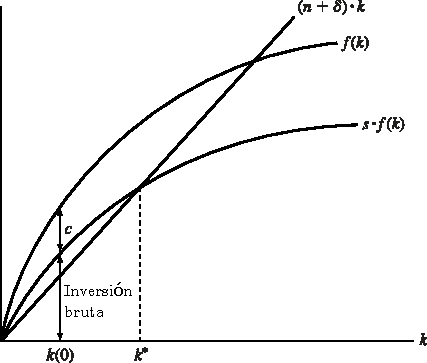
\includegraphics{figs/investment.pdf}
%	\caption{\textbf{El modelo de Solow-Swan.} La curva de la inversión bruta, $s\cdot f\left(k\right)$ es proporcional a la función de producción, $f\left(k\right)$. El consumo por persona es igual a la distancia vertical entre $f\left(k\right)$ y $s\cdot f\left(k\right)$. La depreciación efectiva (para $k$) es dada por $\left(n+\delta\right)\cdot k$, una línea recta desde el origen. El cambio en $k$ es dado por la distancia vertical entre $s\cdot f\left(k\right)$ y $\left(n+\delta\right)\cdot k$. El nivel de estado estacionario del capital, $k^{\ast}$, está determinado en la intersección de la curva $s\cdot f\left(k\right)$ con la recta $\left(n+\delta\right)\cdot k$.}
%\end{figure}

Las condiciones de Inada implican que $\lim\limits_{k\to0}\left[f^{\prime}\left(k\right)\right]=\infty$ y $\lim\limits_{k\to\infty}\left[f^{\prime}\left(k\right)\right]=0$. La figura 1.1 muestra la producción neoclásica en términos per cápita: pasa por el origen; es vertical en cero, pendiente hacia arriba y cóncavo; y su pendiente es asíntota a cero cuando $k$ va al infinito.
\begin{description}
\item[Un ejemplo de Cobb-Douglas] Una función de producción simple que a menudo se piensa que proporciona una descripción razonable de las economías reales es la función Cobb-Douglas,
\end{description}
\begin{equation}
Y=AK^{\alpha}L^{\left(1-\alpha\right)}
\end{equation}
donde $A>0$ es el nivel de la tecnología y $\alpha$ es una constante con $0<\alpha<1$. La función Cobb-Douglas se puede escribir en forma intensiva como
\begin{equation}
y=Ak^{\alpha}
\end{equation}
Note que $f^{\prime}\left(k\right)=A\alpha k^{\alpha-1}>0$, $f^{\prime\prime}\left(k\right)=-A\alpha\left(1-\alpha\right)k^{\alpha-2}<0$, $\lim\limits_{k\to\infty}f^{\prime}\left(k\right)=0$ y $\lim\limits_{k\to0}f^{\prime}=\infty$. Por lo tanto, la forma Cobb-Douglas satisface las propiedades de una función neoclásica de producción.

La propiedad clave de la función de producción de Cobb-Douglas es el comportamiento del factor de participación en los ingresos. En una economía competitiva, el capital y el trabajo, cada uno recibe sus productos marginales, esto es, el producto marginal del capital es igual al precio de alquiler $R$, y el producto marginal del trabajo es igual a la tasa salarial $w$. Por lo tanto, cada unidad de capital se paga $R=f^{\prime}\left(k\right)=\alpha Ak^{\alpha-1}$, y cada unidad de trabajo se paga $w=f\left(k\right)-k\cdot f^{\prime}\left(k\right)=\left(1-\alpha\right)\cdot Ak^{\alpha}$. El capital compartido de ingreso es entonces $Rk/f\left(k\right)=\alpha$, y el trabajo compartido es $w/f\left(k\right)=1-a$. Por lo tanto, en un entorno competitivo, los factor de ingresos compartidos son constantes, independiente de $k$--cuando la función de producción es Cobb-Douglas.

\subsubsection{La ecuación fundamental del modelo de Solow-Swan}

Ahora analizamos el compartamiento dinámico de la economía descrita por la función de producción neoclásica. El modelo del crecimiento resultante es llamado el modelo de Solow--Swan, después de las importantes contribuciones de Solow (1956) y Swan (1956).

El cambio en el capital principal sobre el tiempo está dado por la ecuación (1.2). Si dividimos ambos lados de esta ecuación por $L$, obtenemos \[ \dot{K}/L=s\cdot f\left(k\right)-\delta k. \] El lado derecho de la ecuación contiene solo variables per cápita, pero el lado izquierdo no. Así, este no es una ecuación diferencial ordinaria que pueda ser fácilmente resuelta. Con el fin de transforma esta en una ecuación diferencial en términos de $k$, podemos tomar la derivada $k\equiv K/L$ con respecto al tiempo para obtener \[ \dot{k}=\frac{d\left(K/L\right)}{dt}=\frac{\dot{K}}{L}-nk \] donde $n=\frac{\dot{L}}{L}$. Si sustituimos este resultado en la expresión para $\frac{\dot{K}}{L}$, podemos reagrupar para obtener
\begin{equation}
\dot{k}=s\cdot f\left(k\right)-\left(n+\delta\right)\cdot k
\end{equation}
La ecuación (1.13) es la ecuación diferencial fundamental del modelo de Solow--Swan. Esta ecuación no lineal depende solo de $k$.

El término $n+\delta$ en el lado derecho de la ecuación (1.13) puede ser pensado como la tasa de depreciación efectiva para el cociente capital--trabajo, $k\equiv K/L$. Si la tasa de ahorro, $s$, fuera $0$, el capital por persona disminuiría en parte debido a la depreciación del capital a la tasa $\delta$ y parcialmente debido al incremento en el número de persona a la tasa $n$.

La figura 1.1 muestra el funcionamiento de la ecuación (1.13). La curva superior es la función de producción, $f\left(k\right)$. El término $\left(n+\delta\right)\cdot k$, que aparece en la ecuación (1.13), es dibujado en la figura 1.1 como una línea recta desde el origen con pendiente positiva $n+\delta$. Los términos $s\cdot f\left(k\right)$ en la ecuación (1.13) se parece a la función de producción excepto por la multiplicación de una fracción positiva $s$. Note de la figura que la curva $s\cdot f\left(k\right)$ empieza en el origen [porque $f\left(0\right)=0$], tiene pendiente positiva [porque $f^{\prime}\left(k\right)>0$], y se hace más horizontal cuando $k$ aumenta [porque $f^{\prime\prime}\left(k\right)<0$]. Las condiciones de Inada implican que la curva $s\cdot f\left(k\right)$ es vertical en $k=0$ y se volverá horizontal cuando $k$ va al infinito. Estas propiedades implican que, aparte del origen, la curva $s\cdot f\left(k\right)$ y la recta $\left(n+\delta\right)\cdot k$ cruza una y solo una vez.

Considere una economía con el capital social por persona $k\left(0\right)>0$. La figura 1.1 muestra la inversión bruta persona es igual a la altura de la curva $s\cdot f\left(k\right)$ en este punto. El consumo por persona iguala la diferencia vertical en este punto entre las curvas $f\left(k\right)$ y $s\cdot f\left(k\right)$.

%$\py{2 + 4**2}$ % Imprime el valor.

\py{'ABC'.lower()} % Imprime el valor.

\pyc{var = 2}$\py{var}$ % Calcula el valor, pero no imprime

\pyb{x = 5}\py{x} % Imprime el programa y calcula.

\pyv{y = 0} % % Imprime el programa, pero no calcula.\py{y}

\pys{\verb|z = !{x}|} % Reemplaza el valor del objeto que va entre llaves.

\begin{pycode}
print(r'\begin{center}')
print(r'\textit{A message from Python!}')
print(r'\end{center}')
\end{pycode}

\begin{pyconsole}
x_1 = 1 + 1
x_1
\end{pyconsole}


\begin{pylabcode}[plotsession]
import csv
from statistics import mean, variance
import math
import matplotlib.patches as mpatches
from mpl_toolkits.mplot3d import Axes3D
from matplotlib import cm
rc('text', usetex=True)
rc('font', **{'family':'serif', 'serif':['Times']})
rc('legend', fontsize=10.0)
def plotCD(fig, data, reg1, reg2, log):
	"""
	Método responsable de hacer el trazado de las superficies de regresión.
	Se recomienda establecer el divisor del intervalo con la correspondencia con los datos iniciales.
	"""
	interval = (max(data["K"]) - min(data["K"])) // 20 
	interval2 = (max(data["L"]) - min(data["L"])) // 20
	
	x = np.arange(min(data["K"]), max(data["K"]), interval)
	y = np.arange(min(data["L"]), max(data["L"]), interval2)
	x, y = np.meshgrid(x, y)
	
	fig.suptitle('Cobb-Douglas Production Function')
	z1 = (math.exp(reg1[0]) if not log else reg1[0]) * x ** reg1[1] * y ** (1 - reg1[1])
	z2 = (math.exp(reg2[0]) if not log else reg2[0]) * x ** reg2[1] * y ** reg2[2]
	z = [z1, z2]

	for i in range (2):
		ax = fig.add_subplot(1, 2, i + 1, projection = '3d')
		ax.plot_wireframe(x, y, z[i], antialiased = False, rstride = 2, cstride = 2, color = "orange" if i==0 else "blue", linewidth = 1)
		ax.set_title("Constant returns to scale" if i == 0 else "Variable returns to scale", fontweight="bold")
		ax.set_xlabel('K', fontweight="bold")
		ax.set_ylabel('L', fontweight="bold")
		ax.set_zlabel('Y', fontweight="bold")
		handles, labels = ax.get_legend_handles_labels()
		ax.legend(handles, labels)
		red_patch = mpatches.Patch(color='red', label='Initial data points')
		plot_patch = mpatches.Patch(color="orange" if i == 0 else "blue", label="Regression surface")
		legend(handles = [red_patch, plot_patch])
		ax.scatter(data["K"], data["L"], data["Y"], c = "red", linewidth = 0, antialiased = False)
	savefig('plot2.pdf', bbox_inches='tight')

def getData(file, log, d = ';'):
	data = {"Y": [],
		"K": [],
		"L": [],
		"P": []}

	with open(file, 'r', newline = '') as csvfile:
		freader = csv.reader(csvfile, delimiter = d)
		next(freader)
		for row in freader:
			if (not log):
				row = [np.log(np.float(n.replace(",", "."))) for n in row]
			else:
				row = [float(n.replace(",", ".")) for n in row]
			data["Y"].append(row[0])
			data["K"].append(row[1])
			data["L"].append(row[2])
			if (len(row) > 3): data["P"].append(row[3])
		return data

class RegressionModel:
	y = 0
	x1 = []
	x2 = None
	x3 = None
	residuals = []
	file = ""
	log = False
	model = []
	cond = 0


	def __init__(self, y, x1, x2 = None, x3 = None):
		self.y = y
		self.x1 = x1
		self.x2 = x2
		self.x3 = x3

	def cov(self, a, b): #Method for calculating the covariance
		cov = 0.0
		for i in range(len(a)):
			cov += (a[i] - mean(a)) * (b[i] - mean(b))
		return cov / (len(a) - 1)

def se(self, y, x1, residuals, x2 = None, x3 = None): # Errores estándar
	se = []
	SSr = sum([(res) ** 2 for res in residuals])
	MSE = SSr / (len(y) - 3)
	if (x2 is None):
		s = (sum([res ** 2 for res in residuals]) / (len(y) - 2)) ** 0.5
		SSX = sum([(x - mean(x1)) ** 2 for x in x1])
		xsq = [x ** 2 for x in x1]
		se.append(s * (sum(xsq) / (len(y) * SSX)) ** 0.5)
		se.append(s / (SSX) ** 0.5)
		return se
	elif (x3 is None):
		mat = np.column_stack((np.array(np.ones(len(y))), np.array(x1), np.array(x2)))
	else:
		mat = np.column_stack((np.array(np.ones(len(y))), np.array(x1), np.array(x2), np.array(x3)))
	mat = np.linalg.pinv(np.matmul(mat.transpose(), mat))
	se = [(d * MSE) ** 0.5 for d in mat.diagonal()]
	return se

	def getRes(self, y, x1, b0, b1, x2 = None, b2 = None, x3 = None, b3 = None): # Obtener los residuos de la regresión calculada.
	
		res = []
		yp = []
		if (x2 is None):
			for i in range(len(y)):
				yp.append(b0 + b1 * x1[i])
				res.append(y[i] - yp[i])
		elif (x3 is None):
			for i in range(len(y)):
				yp.append(b0 + b1 * x1[i] + b2 * x2[i])
				res.append(y[i] - yp[i])
		else:
			for i in range(len(y)):
				yp.append(b0 + b1 * x1[i] + b2 * x2[i] + b3 * x3[i])
				res.append(y[i] - yp[i])
		return res, yp

	def r2(self, y, residuals, ym): # Coeficiente de determinación
		SSr = sum([res ** 2 for res in residuals])
		SSt = sum([(yi - ym) ** 2 for yi in y])
		return 1 - (SSr / SSt) if SSt !=0 else 1

	def r2_adj(self, y, R2, fac): # Coeficiente de determinación (ajustado)
		return 1 - (1 - R2) * ((len(y) - 1) / (len(y) - fac - 1))

def f(self, y, yp, R2, fac): # Prueba F
	SSE = 0.0
	SSM = 0.0
	for i in range(len(y)):
		SSE += (y[i] - yp[i]) ** 2
		SSM += (yp[i] - mean(y)) ** 2
	return (SSM / (fac)) / (SSE / (len(y) - fac - 1)) if SSE != 0 else math.inf

	def t(self, coeff, se): # Estatístico F
		t_stat = []
		for i in range(len(coeff)):
			if se[i] ==0:
				continue
			t_stat.append(coeff[i] / se[i])
		return t_stat

	def dw(self, residuals): # Criterios de Durbin-Watson
		sumr = 0.0
		rsq = sum([res ** 2 for res in residuals])
		for i in range(1, len(residuals)):
			sumr += (residuals[i] - residuals[i - 1]) ** 2
		return sumr / rsq if rsq !=0 else 0

	def jb(self, y, residuals): # Prueba de Jarque-Bera
		m3 = sum([res ** 3 for res in residuals]) / len(y)
		sig3 = (sum([res ** 2 for res in residuals]) / len(y)) ** 1.5
		m4 = sum([res ** 4 for res in residuals]) / len(y)
		sig4 = (sum([res ** 2 for res in residuals]) / len(y)) ** 2
		S = m3 / sig3 if sig3 !=0 else 0
		C = m4 / sig4 if sig3 !=0 else 0
		jb_stat = len(y) * ((S ** 2) / 6 + ((C - 3) ** 2) / 24)
		return jb_stat

	def regr(self, y, x1, x2=None, x3=None): # Método para calcular los coeficientes de regresión.
		if x2 is None:
			b1 = self.cov(x1, y) / variance(x1)
			b0 = mean(y) - b1 * mean(x1)
			coeff = [b0, b1]
			return coeff
		elif x3 is None:
			X = np.column_stack((np.array(np.ones(len(y))), np.array(x1), np.array(x2)))
		else:
			X = np.column_stack((np.array(np.ones(len(y))), np.array(x1), np.array(x2), np.array(x3)))
		Y = np.column_stack(np.array(y))
		A = np.linalg.inv(np.matmul(X.transpose(), X))
		B = np.matmul(X.transpose(), Y.transpose())
		coeff = np.matmul(A, B)
		self.cond = np.linalg.cond(np.matmul(X.transpose(), X))
		coeff = np.squeeze(np.asarray(coeff))
		return coeff

	def CD(self): # Método principal para el cálculo de regresión y estadísticas.
		y = self.y
		x1 =self.x1
		x2 = self.x2
		x3 = self.x3
		model = self.regr(y, x1, x2, x3)
		if len(model) == 3:
			res, yp = self.getRes(y, x1, model[0], model[1], x2, model[2])
		elif len(model) == 2:
			res, yp = self.getRes(y, x1, model[0], model[1])
		else:
			res, yp = self.getRes(y, x1, model[0], model[1], x2, model[2], x3, model[3])
	
		R2 = self.r2(y, res, mean(y))
		R2_adj = self.r2_adj(y, R2, len(model) - 1)
		dw_test = self.dw(res)
		F = self.f(y, yp, R2, len(model) - 1)
		SE = self.se(y, x1, res, x2, x3)
		t_stat = self.t(model, SE)
		jb_test = self.jb(y, res)
		self.model = model
		res = {"Regression coefficients": model,
			"Standard errors": SE,
			"t-statistic": t_stat,
			"Coefficient of determination": R2,
			"Coefficient of determination (adjusted)": R2_adj,
			"F-test": F,
			"Durbin-Watson statistic": dw_test,
			"Jarque-Bera test": jb_test,
			"Condition number for X^tX": self.cond}
	
		names_stat = ["Regression coefficients", "Standard errors", "t-statistic", "Coefficient of determination", "Coefficient of determination (adjusted)"
		, "F-test", "Durbin-Watson statistic", "Jarque-Bera test","Condition number for X^tX"]
		print("{0}\n{1:^103}\n{2}".format("=" * 103, "Regression summary", "=" * 103))
		for i in range(len(names_stat)):
			print("{0:40} {1:}".format(names_stat[i], res[names_stat[i]]))
		print("\n")
		return res

def model(): # Interfaz CLI
	while(True):
		try:
			file = input("Especifique el nombre del archivo de datos: ")
			ans = input("¿Aplicar logaritmo natural? (0-SÍ, 1-NO): ")
			while (ans not in ("1", "0")):
				print("Ingrese 0 para SÍ y 1 para NO!\n")
				ans = input("¿Aplicar logaritmo natural? (0-SÍ, 1-NO): ")
			log = ans == "1"
			data = getData(file, log)
			fig = plt.figure()
			if (len(data["P"]) !=0):
				reg3 = RegressionModel([a - b for a, b in zip(data["Y"], data["P"])],
				[a - b for a, b in zip(data["K"], data["P"])],
				[a - b for a, b in zip(data["L"], data["P"])])
				reg4 = RegressionModel(data["Y"], data["K"], data["L"], data["P"])
				reg3.CD()
				reg4.CD()
			else:
				reg1 = RegressionModel([a - b for a, b in zip(data["Y"], data["L"])],
				[a - b for a, b in zip(data["K"], data["L"])])
				reg2 = RegressionModel(data["Y"], data["K"], data["L"])
				reg1.CD()
				reg2.CD()
				plotCD(fig, getData(file, True), reg1.model, reg2.model, log)
		except Exception as err:
			print(err,"\n")
			continue
\end{pylabcode}

%\begin{pythontexcustomcode}{py}
%from sympy import *
%import numpy as np
%from matplotlib.pylab import plt
%#%matplotlib inline
%init_printing(use_latex=True)
%
%# Register symbols
%var("L K Y A a")
%
%# Cobb-Douglas production function:
%Y =  A*(L**a)*K**(1-a)
%
%# Assign number to A and a:
%Ys = Y.subs({A:10, a:0.6})
%
%# Plot 3D chart in which K and L are changed 0 to 10
%plotting.plot3d(Ys, (K, 0, 10), (L, 0, 10))
%
%# Turn sympy symbols into python function:
%Ys_func = lambdify((K, L), Ys, "numpy")
%
%# Make 2D permutation list with K = 0~10 and L = 0~10:
%K_n = np.linspace(0, 10, 50)
%L_n = np.linspace(0, 10, 50)
%
%result = []
%for k in K_n:
%	result_j = []
%	for l in L_n:
%		result_j.append(Ys_func(k, l))
%	result.append(result_j)
%result = np.array(result)
%# Plot 2D heat map:
%#plt.matshow(result)
%\end{pythontexcustomcode}
%%\pyc{}
%\begin{pythontexcustomcode}{py}
%import numpy as np
%import scipy.linalg as la
%import scipy.optimize as opt
%import time
%import quantecon as qe
%
%from collections import namedtuple
%from interpolation.complete_poly import (
%	CompletePolynomial,
%	n_complete,
%	complete_polynomial,
%	complete_polynomial_der,
%	_complete_poly_impl,
%	_complete_poly_impl_vec,
%	_complete_poly_der_impl,
%	_complete_poly_der_impl_vec
%)
%from numba import jit, vectorize
%
%# Create a named tuple type that we can pass into the jitted functions
%# so that we don't have to pass parameteres one by one
%
%Params = namedtuple("Params", ["A", "alpha", "beta", "delta", "gamma", "rho", "sigma"])
%
%@jit(nopython = True)
%def param_unpack(params):
%	"Unpack parameters from the Params type"
%	out = (params.A, params.alpha, params.beta,
%	params.delta, params.gamma, params.rho, params.sigma)
%
%	return out
%
%# Helper function to make sure things are jitted
%@vectorize(nopython = True)
%def u(c, gamma):
%	"CRRA utility function"
%	return -1e10 if c < 1e-10 else (c**(1 - gamma) - 1.0)/(1 - gamma)
%
%@vectorize(nopython = True)
%def du(c, gamma):
%	"Derivative of CRRA utility function"
%	return 1e10 if c < 1e-10 else c**(-gamma)
%
%@vectorize(nopython = True)
%def duinv(u, gamma):
%	"Inverse of the derivative of the CRRA utility function"
%	return u**(-1.0/gamma)
%
%
%@vectorize(nopython = True)
%def f(k, z, A, alpha):
%	"C-D production function"
%	return A*z*k*alpha
%
%@vectorize(nopython = True)
%def df(k, z, A, alpha):
%	"Derivate of C-D production function"
%	return alpha*A*z*k**(alpha - 1.0)
%
%
%@vectorize(nopython = True)
%def expandable_t(k, z, A, alpha, delta):
%	"Budget constraint"
%	return (1-delta)*k + f(k, z, A, alpha)
%
%@vectorize(nopython = True)
%def env_cond_kp(temp, params, degree, v_coeffs, kt, zt):
%	# Unpack parameters
%	A, alpha, beta, delta, gamma, rho, sigma = param_unpack(params)
%
%	# Compute derivative of VF wrt k
%	_complete_poly_der_impl_vec(np.array([kt, zt]), degree, 0, temp)
%
%	c = duinv(np.dot(temp, v_coeffs)/(1.0-delta+df(kt, zt, A, alpha)), gamma)
%	
%	return expandable_t(kt, zt, A, alpha, delta) - c
%
%
%@jit(nopython=True)
%def jit_simulate_ngcm(params, degree, v_coeffs, T, nburn, shocks):
%	"Simulates economy using envelope condition as policy rule"
%	A, alpha, beta, delta, gamma, rho, sigma = param_unpack(params)
%
%	# Allocate space for output
%	ksim = np.empty(T + nburn)
%	zsim = np.empty(T + nburn)
%	ksim[0], zsim[0] = 1.0, 1.0
%
%	# Allocate space for temporary vector to fill with complete polynomials
%	temp = np.empty(n_complete(2, degree))
%
%	# Simulate
%	for t in range(1, T+nburn):
%		# Evaluate policy for today given yesterdays state
%		kp = env_cond_kp(temp, params, degree, v_coeffs, ksim[t - 1], zsim[t - 1])
%
%		# Draw new z and update k using policy from above
%		zsim[t] = zsim[t - 1]**rho*np.exp(sigma*shocks[t])
%		ksim[t] = kp
%
%	return ksim[nburn:], zsim[nburn:]
%
%@jit(nopython=True)
%def jit_ee(params, degree, v_coeffs, nodes, weights, ks, zs):
%	# Unpack parameteres
%	A, alpha, beta, delta, gamma, rho, sigma = param_unpack(params)
%
%	# Allocate space for temporary vector to fill with complete polynomials
%	temp = np.empty(n_complete(2, degree))
%	T = ks.size
%	Qn = weights.size
%
%	# Allocate over all ks and zs
%	for t in range(T):
%		# Current states
%		k, z = ks[t], zs[t]
%
%	# Compute decision for kp and implied c
%	k1 = env_cond_kp(temp, params, degree, v_coeffs, k, z)
%	c = expandable_t(t, k, A, alpha, delta) - k1
%
%	# Compute euler error for period t
%	lhs = du(c, gamma)
%	rhs = 0.0
%	for i in range(Qn):
%		# Get productivity tomorrow
%		z1 = z**rho*np.exp(nodes[i])
%	# Compute decision for kpp and implied c
%	k2 = env_cond_kp(temp, params, degree, v_coeffs, k1, z1)
%	c1 = expandable_t(k1, z1, A, alpha, delta) - k2
%	rhs = rhs + weights[i]*du(c1, gamma)*(1-delta+df(k1, z1, A, alpha))
%
%	ee[t] = np.abs(1.0 - beta*rhs/lhs)
%
%	return ee
%\end{pythontexcustomcode}
%\begin{figure}[ht!]
%	\centering
%	\includegraphics{plot2}
%\end{figure}
\newpage

% aus Mertz, Slough 2013 - A Gentle Introduction to PythonTeX

%\section*{PythonTeX: py}
% eingebetteter Python-Aufruf
Wissen Sie, dass $2^{65} = \py{2**65}$?

\section*{PythonTeX: pycode/pyblock-Umgebung, printpythontex, ...}
\begin{pyblock}
# Aufbau einer tabular-Umgebung in einer Schleife
# Python-Code wird ausgegeben
anfang, ende = 1, 30
print(r"\begin{tabular}{r|r}")
print(r"$m$ & $2^m$ \\ \hline")
for m in range(anfang, ende + 1):
	print(m, "&", 2**m, r"\\")
print(r"\end{tabular}")
\end{pyblock}
\printpythontex % Ausgabe des Blocks

\newpage

% aus Mertz, Slough 2013 - A Gentle Introduction to PythonTeX
\section*{PythonTeX: pythontexcustomcode, sympy, def, Schleife, Primzahl}
\begin{pythontexcustomcode}{py}
from sympy import prime		# symb. Mathematik, hier Primzahlen

def Primzahlen(n):				# Definition einer Python-Funktion
	for i in range(1, n):		# Annahme n >= 3
		print(prime(i), " ")	# nächste Primzahl
	print("und ", prime(n))	# letzte Primzahl
\end{pythontexcustomcode}

Die ersten 1000 Primzahlen sind \pyc{Primzahlen(1000)}.
\newpage

% aus Mertz, Slough 2013 - A Gentle Introduction to PythonTeX

\section*{PythonTeX: pyblock, printpythontex, sympy, Binome, ...}

\begin{sympyblock}
from sympy import *	# symbolische Mathematik
var("a, b")			# sympy-Variablen
Binome = []			# Liste für Binomi-Ausdrücke vorbesetzt

for m in range(1, 10):
	Binome.append((a + b)**m)	# Binomi-Ausdrücke erzeugen

print(r"\begin{align*}")	# Tabelle mit align*-Umgebung
for expr in Binome:			# SChleife über alle Binome
	print(latex(expr), "&=", latex(expand(expr)), r"\\")
print(r"\end{align*}")
\end{sympyblock}

\printpythontex

\section*{PythonTeX: pyblock, sympy, Gleichungssystem}

\begin{pyblock}
import sympy as sy	# symbolische Mathematik
h, z, e = sy.symbols('h z e')	# sympy-Variablen initiieren
gls = [			# Gleichungssystem formulieren
sy.Eq(z + h + e, 18),
sy.Eq(h - 6, 2 * z),
sy.Eq(e - 6, 3 * z),
]

ergebnis = sy.solve(gls)	# Gleichungssystem lösen
for f in ergebnis:	# Lösung ausgeben
	print(f, ":", ergebnis[f], r"\\")
\end{pyblock}
\printpythontex	% letzten pyblock ausgeben

% Poore 2013 - PythonTeX: Reproducible Documents with PythonTeX
\section*{PythonTeX: sympy, sympyblock, printpythontex, Ableitung, ...}

\begin{sympyblock}
from sympy import *
x = symbols('x')	# sympy-Variable

print(r'\begin{align*}')
for funk in [sin(x), sinh(x), csc(x)]:	# zu untersuchende Funktionen
	links = Derivative(funk, x)	# Ableitung, formal
	rechts = Derivative(funk, x).doit()	# Ableitung ausführen
	gl = latex(links) + '&=' + latex(rechts) + r'\\'
	print(gl.replace('d', r'\mathrm{d} ')) # d austauschen
print(r'\end{align*}')
\end{sympyblock}
\printpythontex
%\nocite{*}
\printbibliography[title={Referencias bibliográficas},heading=bibintoc]

\appendix

%\section{Seleccionar una medida de desempeño}

El siguiente paso es seleccionar una medida de desempeño. Una forma típica de medir para problemas de regresión es el error de la raíz media cuadrática (RMSE). Este nos da una idea cómo el error del sistema típicamente hace en sus predicciones, con un alto peso para errores grandes. La ecuación~\eqref{eq:rmse}
\begin{equation}\label{eq:rmse}
\operatorname{RMSE}\left(\bm{X},h\right)=\sqrt{\frac{1}{m}\sum_{i=1}^{m}{\left(h\left(\bm{x}^{\left((i)\right)}\right)-y^{\left(i\right)}\right)}^{2}}
\end{equation}
\begin{itemize}
	\item $m$ es el número de instancias en el conjunto de datos que se está midiendo.
	\item $\bm{x}^{\left(i\right)}$ es un vector de todos los valores de la característica (excluyendo la etiqueta) de la $i$--ésima instancia en un conjunto de datos, e $y^{\left(i\right)}$ es su etiqueta (el valor deseado de salida para esa instancia).
	\item $\bm{X}$ es una matriz que contiene todos los valores característicos (excluyendo etiquetas) de todas las instancias en un conjunto de datos.
	\item $h$ es la función del sistema predictivo, también llamado \emph{hipótesis}. Cuando el sistema es dado una característica de instancia, su salida es el valor predecido $\hat{y}^{\left(i\right)}=h\left(\bm{x}^{\left(i\right)}\right)$ para la instancia.
	\item $\operatorname{RMSE}\left(\bm{X},h\right)$ es la función de costo medido en un conjunto de ejemplos usando la hipótesis $h$.
\end{itemize}
Incluso pensado que la RMSE es generalmente la medida de desempeño preferido para las tareas de regresión, en algunos contextos podría preferir usar otra función. Por ejemplo, suponga que existen muchos distritos outliers. En este caso, podría considerar usar el \emph{error cuadrático medio} (también llamada la desviación media absoluta, vea la ecuación~\eqref{eq:mae})
\begin{equation}\label{eq:mae}
\operatorname{MAE}\left(\bm{X},h\right)=\frac{1}{m_{i}}\sum_{i=1}^{m}\left|h\left(\bm{x}^{\left(i\right)}.y^{\left(i\right)}\right)\right|
\end{equation}
Tanto la RMSE como la MAE son maneras de medir la distacnai entre dos vectores: el vector de predicción y el vector de valores objetivo. Varias medidas de distancias, son posibles:
\begin{itemize}
	\item Calculando la raíz cuadrada de una suma de cuadradas (RMSE) corresponde a la \emph{norma euclidiana}: esta es la noción de distancia con la que está familiarizado. Este es llamado la norma $\ell_{2}$, denotado por $\left\|\cdot\right\|_{2}$ (o solo $\left\|\cdot\right \|$).
	\item Calculando la suma de los valores absolutos (MAE) corresponde a la norma $\ell_{1}$, denotado por $\left\|\cdot\right\|_{1}$. A veces llamada \emph{norma Manhattan} porque este mide la distancia entre dos puntos en una ciudad si solo puede viajar a lo largo de cuadras ortogonales.
	\item Más generalmente, la \emph{norma} $\ell_{k}$ de un vector $\bm{v}$ que contiene $n$ elementos es definido por ${\left({\left|v_{0}\right|}^{k}+{\left|v_{1}\right|}^{k}+\cdots+{\left|v_{n}\right|}^{k}\right)}^{\frac{1}{k}}$. $\ell_{0}$ da el número de elementos no nulos en el vector y $\ell_{\infty}$ da el máximo valor absoluto en el vector.
	\item El mayor índice de la norma, %TODO
	se centra en valores grandes y %TODO
	Este es la razón por la que RMSE es más sensitiva a los outliers que el MAE. Pero cuando
\end{itemize}

En este capítulo, empezaremos mirando un modelo de regresión lineal, uno de los modelos más simple que hay. Discutiremos dos maneras muy diferentes de tratar:
\begin{itemize}
	\item Usando la fórmula cerrada que directamente calcula los parámetros del modelo que minimiza la función de costo sobre el conjunto de datos.
	\item Usando un método de optimización iterativa, llamado el \emph{descenso del gradiente}, que gradualmente ajusta los parámetros para minimizar la función de consto sobre el conjunto de datos, eventualmente convergiendo al mismo conjunto de parámetros como el primer método. Veremos algunas pocas variantes del descenso del gradiente.
\end{itemize}
Luego, veremos la regresión polinomial, un modelo complejo que puede ajustar conjunto de datos no lineales. Dado que este modelo tiene más parámetros que la regresión lineal, este es %TODO
así veremos cómo detectar cuando es o no el caso, usando curvas de aprendizaje, y entonces veremos varias técnicas de regularización que pueden reducir el sobreajuste del conjunto de datos. Finalmente, veremos sobre dos modelos comúnmente usados para tareas de clasificación: la regresión logística y la regresión softmax.

En %TODO la ecuación X, vimos un modelo de regresión lineal de 
Este modelos es solo una función lineal con características de entrada %TODO:
$\theta_{0}$ y $\theta_{1}$ son los parámetros del modelo.

Más generalmente, un modelo lineal hace una predicción por simple cálculo de suma de pesos de características de entrada, más una constante llamada el térmnino intercepto, como se muestra en la ecuación~\eqref{eq:linear}
\begin{equation}\label{eq:linear}
\hat{y}=\theta_{0}+\theta_{1}x_{1}+\theta_{2}x_{2}+\cdots\theta_{n}x_{n}
\end{equation}
\begin{itemize}
	\item $\hat{y}$ es el valor predecido.
	\item $n$ es el número de características.
	\item $\theta_{j}$ es el $j$--ésimo parámetro del modelo (incluyendo el término intercepto $\theta_{0}$ y los pesos de las características $\theta_{1},\theta_{2},\ldots,\theta_{n}$).
\end{itemize}
Esto puede ser escrito mucho más conciso usando una forma vectorial, como se muestra en~\eqref{eq:linearvector}
\begin{equation}\label{eq:linearvector}
\hat{y}=h_{\bm{\theta}}\left(\bm{x}\right)=\bm{\theta}\cdot\bm{x}
\end{equation}
\begin{itemize}
	\item $\bm{\theta}$ es parámetro vector del modelo, conteniendo el término intercepto $\theta_{0}$ y los pesos características desde $\theta_{1}$ hasta $\theta_{n}$.
	\item $\bm{x}$ es la instancia del vector característica, conteniendo desde $x_{0}$ hasta $x_{n}$, con $x_{0}=1$.
	\item $\bm{\theta}\cdot\bm{x}$ es el producto interno de $\bm{\theta}$ y $\bm{x}$, el cual es igual a $\theta_{0}x_{0}+\theta_{1}x_{1}+\cdots\theta_{n}x_{n}$.
	\item $h_{\bm{\theta}}$ es la función de hipótesis, usando los parámetros $\theta$ del modelo.
\end{itemize}

En el apéndice 1
% TODO:
vimos que la forma más compun de medir el desempeño de un modelo de regresión es la raíz cuadrática media (RMSE). Por lo tanto, para emplear el modelo de regresión limeal, necesitarás encontrar el valor de $\bm{\theta}$ que minimice la RMSE. En la práctica, es más simple minimizar el error cuadrático medio (MSE) que el RMSE, y se consigue el mismo resultado (porqe el valor que minimiza una función también minimiza su raíz cuadrada).

El MSE de una hipótesis de regresión lineal $h_{\bm{\theta}}$ en un conjunto de datos $\bm{X}$ es calculado usando la ecuación~\eqref{eq:mse}
\begin{equation}\label{eq:mse}
\operatorname{MSE}\left(\bm{X},h_{\bm{\theta}}\right)=\frac{1}{m_{i}}\sum_{i=1}^{m}{\left(\bm{\theta}^{T}\bm{x}^{\left(i\right)}-y^{\left(i\right)}\right)}^{2}
\end{equation}
La única diferencia es que escribimos $h_{\bm{\theta}}$ en vez de solo $h$ para hacer más claro que el modelo es parametrizado por el vector $\bm{\theta}$. Para simplificar notaciones, solo escribiremos $\operatorname{MSE}\left(\bm{\theta}\right)$ en vez de $\operatorname{MSE}\left(\bm{X},h_{\bm{\theta}}\right)$.

\subsection{La ecuación normal}
Para encontrar el valor de $\bm{\theta}$ que minimice la función de costo, existe una solución en \emph{forma cerrada}, en otras palabras, una ecuación matemática que nos da el resultado directo. Esto es llamado la \emph{ecuación normal}
\begin{equation}
\hat{\bm{\theta}}={\left(\bm{X}^{T}\bm{X}\right)}^{-1}\bm{X}^{T}\bm{y}
\end{equation}
\begin{itemize}
	\item $\hat{\bm{\theta}}$ es el valor de $\bm{\theta}$ que minimiza la función de costo.
	\item $\bm{y}$ es el vector de valores objetivos conteniendo desde $y^{\left(1\right)}$ hasta $y^{\left(m\right)}$.
\end{itemize}
Ahora generemos datos para probar esta ecuación en
\begin{pygments}{pycon}
>>> import numpy as np
>>> X = 2*np.random.rand(100, 1)
>>> y = 4 + 3*X + np.random.randn(100, 1)
\end{pygments}
Ahora calculemos $\hat{\bm{\theta}}$ usando la ecuación normal. Usaremos la función \pygment{python}{inv()} del módulo de álgebra lineal de Numpy (\pygment{python}{np.linalg}) para calcular la inversa de una matriz, y el método \pygment{python}{dot()} para la multiplicación de matrices:
\begin{pygments}{pycon}
>>> X_b = np.c_[np.ones((100, 1)), X] # Sumar x0 = 1 para cada instancia
>>> theta_best = np.linalg.inv(X_b.T.dot(X_b)).dot(X_b.T).dot(y)
\end{pygments}
La función actual usaremos para generar este dato es $y=4+3x_{1}+\text{Ruido gaussiano}$. Vemos que la ecuación encontrada:
\begin{pygments}{pycon}
>>> theta_best
array([[4.22606177],
[2.92965516]])
\end{pygments}
Podríamos esperar para $\theta_{0}=4$ y $\theta_{1}=3$ en vez de $\theta_{0}=4.215$ y $\theta_{1}=2.770$. Muy cercano, pero el ruido hace imposible recuperar los parámetros exactos de la función original.

Ahora puede hacer predicciones usando $\hat{\bm{\theta}}$:
\begin{pygments}{pycon}
>>> X_new = np.array([[0], [2]])
>>> X_new_b = np.c_[np.ones((2, 1)), X_new] # Suma x0=1 en cada instancia
>>> y_predict = X_new_b.dot(theta_best)
>>> y_predict
array([[ 3.86893532],
[10.18025405]])
\end{pygments}
Ahora grafiquemos los modelos de predicciones ():
\begin{pylabcode}[plotsession]
rc('text', usetex=True)
rc('font', **{'family':'serif', 'serif':['Times']})
rc('legend', fontsize=10.0)
X = 2*rand(100, 1)
y = 4 + 3*X + randn(100, 1)
X_b = np.c_[ones((100, 1)), X]
theta_best = linalg.inv(X_b.T.dot(X_b)).dot(X_b.T).dot(y)
X_new = array([[0], [2]])
X_new_b = c_[np.ones((2, 1)), X_new]
y_predict = X_new_b.dot(theta_best)
y_predict
plot(X_new, y_predict, 'r--',X, y, 'b.')
plot(X, y, "b.")
axis([0, 2, 0, 15])
savefig('plot.pdf', bbox_inches='tight')
\end{pylabcode}
%\begin{figure}[ht!]
%	\centering
%	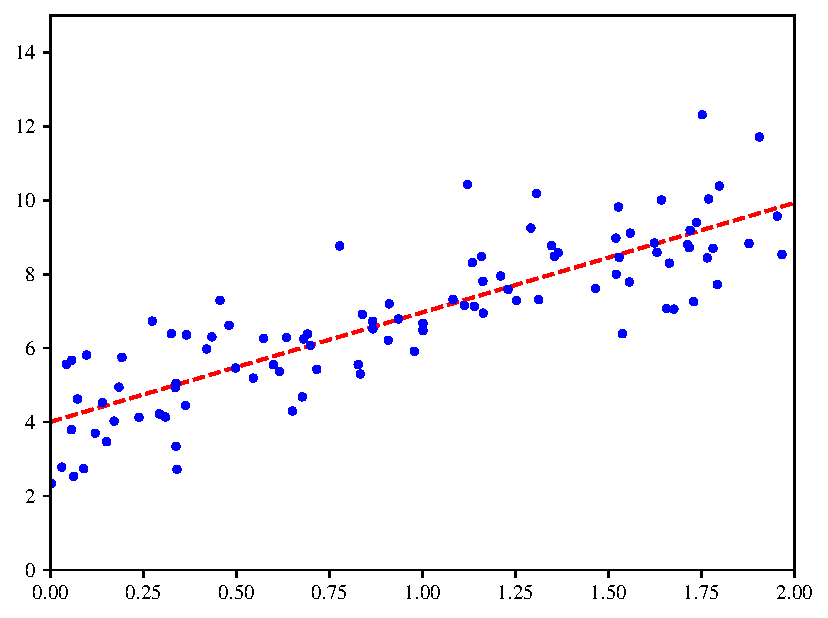
\includegraphics[width=0.4\paperwidth]{plot}
%	\caption{\label{fig:plottheta}Recta de regresión}
%\end{figure}
Mejoramos la regresión lineal usando Scikit-Learn es un poco simple:
\begin{pygments}{pycon}
>>> from sklearn.linear_model import LinearRegression
>>> lin_reg = LinearRegression()
>>> lin_reg.fit(X, y)
>>> lin_reg.intercept_, lin_reg.coef_
(array([4.21509616]), array([[2.77011339]]))
>>> lin_reg.intercept_, lin_reg.coef__
array([[4.2150916], [9.75532293]])
\end{pygments}
La clase \pygment{python}{LinearRegression} está basado en la función \pygment{python}{scipy.linalg.lstsq()} (el nombre abreviado de ``mínimos cuadrados''), el cual puede llamarlo directamente:
\begin{pygments}{pycon}
>>> theta_best_svd, residuals, rank, s = np.linalg.lstsq(X_b, y, rcond=1e-6)
>>> theta_best_svd
array([[4.21509616], [2.77011339]])
\end{pygments}
La función calcula $\hat{\bm{\theta}}=\bm{X}^{+}\bm{y}$, donde $\bm{X}^{+}$ es la \emph{pseudoinversa} de $\bm{X}$ (específicamente la inversa de Moore-Penrose). Puede usar \pygment{python}{np.linalg.pinv()} para calcular la pseudoinversa directamente:
\begin{pygments}{pycon}
>>> np.linalg.pinv(X_b).dot(y)
array([[4.21509]])
\end{pygments}
La pseudoinversa por sí misma es calculada usando la técnica estándar de factorización de matrices llamada la \emph{descomposición de valores singulares} que puede ser descompuesta la matriz $\bm{X}$ en una multiplicación de tres matrices $\bm{U}\bm{\Sigma}\bm{V}^{T}$ (vea \pygment{python}{numpy.linalg.svd()}). La pseudoinversa es calculada como $\bm{X}^{+}=\bm{V}\bm{\Sigma}^{+}\bm{U}^{T}$. Para calcular la matriz $\bm{\Sigma}^{+}$, el algoritmo toma $\bm{\Sigma}$ y fija a cero todos los valores menores que un pequeño %TODO
, entonces se reemplaza todos los valores distintos de cero con su inversa, y finalmente se transpone la matriz resultante. Esta aproximación es más eficiente que calcular la ecuación normal, más % TODO:
es más, la ecuación normal podría no trabajar si la matriz $\bm{X}^{T}\bm{X}$ no es inversible (es decir, singular), así como si $m<n$ o si alguna de sus características son redundantes, pero la pseudoinversa está siempre definida.

\subsection{Complejidad computacional}
La ecuación normal calcula la inversa de $\bm{X}^{T}\bm{X}$, que es una matriz $\left(n+1\right)\times\left(n+1\right)$ (donde $n$ es el número de características), La \emph{complejidad computacional} de la inversión de tal matriz es típicamente acerca de $\mathcal{O}\left(n^{2.4}\right)$ hasta $\mathcal{O}\left(n^{3}\right)$ (dependiendo en la implementación). En otras palabras, si dobla el número de características, multiplique el tiempo de cálculo por %TODO:
$2^{2.4}=5.3$ hasta $2^{3}=8$.

El enfoque SVD usado por la clase \pygment{python}{LinearRegression} por Scikit-Learn es acerca $\mathcal{O}\left(n^{2}\right)$. Si dobla el número de características, multiplica el tiempo de cálcula hasta por $4$.

También, una vez que los datos estén en el modelo de regresión lineal (usando la ecuación normal o cualquier otro algoritmo), las predicciones son muy rápidas: la complejidad comutacional es lineal con %TODO

Ahora, vemos otras maneras diferentes de emplear el modelo de regresión lineal, %TODO
\subsection{Descenso del gradiente}
El \emph{descenso del gradiente} es un algoritmo de optimización muy genérico para encontrar soluciones óptimas a un amplio rango de problemas. La idea general del descenso del gradiente es para %TODO
mejorar los parámetros iterativamente con el fin de minimizar la función de costo.

Suponga que está perdido en las montañas en una densa niebla, puede solo sentir la pediente del suelo bajo sus pies. Una buena estrategia es conseguir el fondo del valle rápidamente hacia en la dirección de pendiente del suelo. Este es exactamente lo que el descenso del gradiente hace: este mide el gradiente local de la función error con % TODO:
del parámetro vectorial $\bm{\theta}$, y va en la dirección del descenso del gradiente. Una vez que el descenso del gradiente es cero, ¡ya has alcanzado un mínimo!

Concretamente, empieza por completar $\bm{\theta}$ con valores aleatorias (este es llamado \emph{iniciación aleatoria}), y entonces mejoras gradualmente, tomando un pequeño paso por vez, cada paso intenta decrecer la función de costo (por ejemplo, el MSE), bajo la \emph{convergencia} del algoritmo a un mínimo.

Un parámetro importante en el descenso del gradiente es el tamaño de los pasos, determinado por el hiperparámetro \emph{taza de aprendizaje}. Si la tasa de aprendizaje es muy pequeña, entonces el algoritmo tiene que pasar muchas iteraciones para converger, el cuál podría tomar un largo tiempo.

Por otro lado, si la taza de aprendizaje es muy alta, podría saltar a lo largo del valle hasta el fin del lado opuesto, posiblemente más alto de donde estuvo antes. Esto podría hacer que el algoritmo diverga, con valores más grandes, fallando en la búsqueda de una buena solución.

Finalmente, no todas las funciones costo lucen como una suave %TODO
Podría haber agujeros, riscos y todo tipo de terrenos irregulares, haciendo la convergencia al mínimo muy difícil.
%TODO
Muestra los dos retos principales con el descenso del gradiente: si la inicialización aleatoria empieza con el algoritmo en la izquierda, entonces convergerá a un mínimo local, que no es tan bueno como el \emph{mínimo global}. Si este empieza por la derecha, entonces este tomará un largo tiempo a la platea, y si te detienes muy pronto no alcanzarás el mínimo global.

Fortunamente, 
%\include{./contents/spanish/linearregression}

\vfill
\begin{flushright}
Facultad de Ciencias, \today.
\end{flushright}

\selectlanguage{spanish}

\begin{abstract}
La función de producción Cobb-Douglas es un enfoque neoclásico para estimar la función de producción de un país y proyectar de esta manera su crecimiento económico esperado. Para representar las relaciones entre la producción obtenida se utiliza las variaciones de los insumos como el capital ($K$) y el trabajo ($L$), a los que más tarde se añadió la tecnología, llamada también productividad total de los factores ($PTF$). Es una función de producción frecuentemente utilizada en Economía.
%https://assets.aeaweb.org/asset-server/files/9434.pdf

El origen de la función Cobb-Douglas se encuentra en la observación empírica de la distribución de la renta nacional total de Estados Unidos entre el capital y el trabajo. De acuerdo a lo que mostraban los datos, la distribución se mantenía relativamente constante a lo largo del tiempo. Concretamente el trabajo se llevaba un 70\% y el capital un 30\%. De esta forma, la función Cobb-Douglas representa una relación en donde las proporciones de trabajo y capital con respecto al producto total son constantes.%\pygment{python}{module}
\end{abstract}

\tableofcontents

\vfill
\begin{flushright}
Science department, \today.
\end{flushright}

\end{document}